\documentclass{article}

%% Conditional revision of November 2026: six pages of main text, from the title to the end of Section 7 (label
%% fine-testo); the Limitations, the AI usage statement, the references and the appendices do not count.
%% Final mode with the workshop name. Line numbers on every fifth line, small and grey, for the note to the
%% program chairs, who asked for section and line numbers. Copy without them: pdflatex "\def\cleancopy{}\documentclass{article}

%% Conditional revision of November 2026: six pages of main text, from the title to the end of Section 7 (label
%% fine-testo); the Limitations, the AI usage statement, the references and the appendices do not count.
%% Final mode with the workshop name. Line numbers on every fifth line, small and grey, for the note to the
%% program chairs, who asked for section and line numbers. Copy without them: pdflatex "\def\cleancopy{}\documentclass{article}

%% Conditional revision of November 2026: six pages of main text, from the title to the end of Section 7 (label
%% fine-testo); the Limitations, the AI usage statement, the references and the appendices do not count.
%% Final mode with the workshop name. Line numbers on every fifth line, small and grey, for the note to the
%% program chairs, who asked for section and line numbers. Copy without them: pdflatex "\def\cleancopy{}\documentclass{article}

%% Conditional revision of November 2026: six pages of main text, from the title to the end of Section 7 (label
%% fine-testo); the Limitations, the AI usage statement, the references and the appendices do not count.
%% Final mode with the workshop name. Line numbers on every fifth line, small and grey, for the note to the
%% program chairs, who asked for section and line numbers. Copy without them: pdflatex "\def\cleancopy{}\input{main}".
%% Every line numbered (same numbering, used to find the lines cited in the note): "\def\everyline{}\input{main}".
\usepackage[final,sglblindworkshop]{neurips_2026}
\workshoptitle{AIMO Interpretability Challenge}
\ifdefined\cleancopy\else
  \usepackage{lineno}
  \linenumbers
  \ifdefined\everyline\else\modulolinenumbers[5]\fi
  \renewcommand\linenumberfont{\normalfont\tiny\sffamily\color{black!45}}
\fi

\usepackage[utf8]{inputenc}
\usepackage[T1]{fontenc}
%% Typewriter text in Latin Modern, the Type 1 version of the default Computer Modern typewriter, with the same
%% widths: without it, \texttt in T1 encoding becomes bitmap (Type 3) fonts, and the template asks for Type 1 fonts.
\renewcommand{\ttdefault}{lmtt}
\usepackage{hyperref}
\hypersetup{pdftitle={The Instrument Behind the Leaderboard: Re-Execution Noise and Label Regeneration in the AIMO Interpretability Challenge}, pdfauthor={Daniel Culotta}}
\usepackage{url}
\def\UrlBreaks{\do\/\do\.\do\_\do\-\do\:}
\usepackage{booktabs}
\usepackage{array}
\usepackage{longtable}
\newcolumntype{L}[1]{>{\raggedright\arraybackslash}p{#1}}
\usepackage{amsfonts}
\usepackage{microtype}
\usepackage{xcolor}
\usepackage{graphicx}
\usepackage{enumitem}
\usepackage{needspace}
\setlist[itemize]{leftmargin=1.4em, itemsep=2pt, topsep=4pt, parsep=0pt}
\setlist[itemize,2]{label=$\circ$}
\renewcommand{\arraystretch}{1.15}
\raggedbottom

\title{The Instrument Behind the Leaderboard: Re-Execution Noise and Label Regeneration in the AIMO Interpretability Challenge}

\author{%
  Daniel Culotta \\
  Independent researcher
}

\begin{document}

\maketitle

\begin{abstract}
We treat the AIMO Interpretability benchmark, which asks whether a model's answer to a math problem survives perturbations, as a measurement instrument. Almost all our label and probe analyses use the preliminary datasets. As the program chairs note, these differ from the official training and validation data in sampling, perturbations and eligibility, so findings on label reliability and predictability may not hold in the official evaluation. First, on DeepSeek-R1-0528-Qwen3-8B in the official pipeline, 24 of 40 items changed prediction across five default runs. Turning compilation off, or deterministic algorithms on, gave three byte-identical runs, each on one card. Second, we regenerated labels with our own protocol, not the official one: our perturbations and answer key, one answer per variant, a 16,384-token cap and temperature 0.6, where the organizers publish 100,000 tokens and 1.0. Two independent draws agree at kappa 0.35 to 0.44 on three of four models however truncated chains are treated, and 0.18 to 0.44 on Qwen3.5-4B, whose chains often reach the cap. Draw A agrees with the 138 published DeepSeek labels at kappa 0.01. This describes our protocol and does not measure the reliability of the organizers' labels. Third, of the 27 dated hypotheses with a kill criterion, 21 failed it. Our probe on DeepSeek's hidden states does no better than problem length (AUROC 0.710 against 0.704; below length on the published labels) and adds nothing detectable to it.
\end{abstract}

\section{Introduction}\label{sec:1}

A leaderboard is a measurement. Its score is read off an instrument made of a label, an evaluation set, an inference pipeline and the hardware it runs on. When the label is itself produced by a stochastic process, the instrument has noise of its own, which a single submission cannot see. We measure the re-execution noise of the official extraction and regressor, and the repeatability of labels regenerated with our own protocol, not the noise of the organizers' labels.

We study the instrument of the AIMO Interpretability Challenge, in which a submission predicts, for a given model and math problem, whether the model's answer is robust to perturbations of the problem [1]. We ran our work as a falsification campaign: every hypothesis was recorded in a dated file, 26 of the 31 before their data were seen, and every tested hypothesis is reported. Of the 31 entries, 27 carried a kill criterion written before their test ran (for 3 of them in a written plan rather than a frozen pre-registration, and for H2 after its concordance had been seen). By that criterion 21 were rejected, 5 survived and 1 is not established (Appendix~\ref{app:A}).

\paragraph{Scope.} Three limits apply.
\begin{itemize}
\item \textbf{Preliminary and official data.} Almost all of our label and probe analyses use the six preliminary public datasets released before the main phase. Their labels follow an earlier rule than those of the official training set (\texttt{train-main-v2}) and of the validation and test tasks [5]; as the program chairs noted in their meta-review, their sampling procedures, perturbations and eligibility criteria also differ. Beyond the label rule, we did not compare the two. Unless we say otherwise, a result on labels or on their predictability holds for the preliminary data and may not hold in the official evaluation setting.
\item \textbf{Our labeling protocol is not the official one.} When we regenerate labels (Section~\ref{sec:labels}), we use our own perturbations, prompts, sampling, decoding, answer key and labeling rule. Disagreement with the organizers' preliminary labels therefore shows that the two processes give different labels; it does not establish that their labels are unreliable or irreproducible.
\item \textbf{Mostly one model.} The re-execution study of Section~\ref{sec:reexec}, the probe analyses and every comparison of our regenerated labels with the organizers' preliminary labels are on DeepSeek-R1-0528-Qwen3-8B. Regenerated labels cover four models, but no conclusion about the official benchmark is established across models.
\end{itemize}

Within these limits, Sections~\ref{sec:reexec} to~\ref{sec:campaign} report re-execution noise and two candidate remedies, our regenerated labels, and signals that do no better than problem length or come from an artifact of the data. Nondeterminism of LLM inference is documented in general [2, 3]; we add its size for one model, one submission and 40 problems on this benchmark's hardware and pipeline. We make no claim about any participant's method.

\section{The task, the labels and the data}\label{sec:data}

\paragraph{Task.} A submission receives a model identifier, a reasoning effort and a list of problems, and returns one robustness verdict per problem, offline on one GPU within one hour [4, 5], or 70 minutes since 15 October [6]. The models are Qwen3.5-4B, Skywork-OR1-Math-7B, Olmo-3-7B-Think and \mbox{DeepSeek-R1-0528-Qwen3-8B} in both tracks, and gpt-oss-120b in the Main track only.

\paragraph{Official data.} The main-phase training set \texttt{train-main-v2} labels all five models with a threshold on the largest accuracy drop across perturbation families: robust at most 0.10, non-robust at least 0.25, no label in between [5]. The organizers' published decoding settings are up to 100,000 tokens at temperature 1.0, top-k 40 and top-p 0.95, and a response that reaches the limit without a final answer counts as wrong [4]. Since 16 September the private validation tasks have 21 items (Main) and 14 (Small), on which the binomial standard error of an accuracy near one half is 10.9 and 13.4 points; the final test uses 30 to 50 new problems [5, 6].

\paragraph{Preliminary data.} Six datasets released before the main phase aggregate to 335 (model, problem) pairs over 174 distinct problems, up to eight per problem; 52 pairs repeat the DeepSeek measurements under a second model name. Their labels follow an earlier rule: on all 379 labeled rows (a pair can have several), the label equals the conjunction ``no perturbation lowered accuracy''. A per-family majority rule (``more than half of the answers are correct in every perturbation family'') reproduces the same 379 labels, so these rows cannot tell the two rules apart. Whether they used the decoding settings above is not documented; in the files behind most DeepSeek labels, most variants listed as lowering accuracy were answered 10 times. We call their labels the organizers' preliminary labels, and keep ``official'' for \texttt{train-main-v2} and the validation and test tasks.

\paragraph{DeepSeek labels.} DeepSeek is the only evaluated model with many preliminary labels: 164 distinct problems (the 52 duplicated pairs count once). For 138 of them the data publish a label. For the other 26 we derived one with the conjunction, which makes 4 of them robust; the majority rule would make 21 robust, so these 26 labels depend on the choice of rule. We therefore report results on the 138 published labels separately.

\section{Re-execution noise on the evaluation workers' type of GPU}\label{sec:reexec}

On a virtual machine lent by the organizers, with two NVIDIA RTX PRO 6000 Blackwell Server Edition GPUs (the type the evaluation workers use), we ran 40 preliminary public problems through the official runtime image, extraction and regressor, unmodified, on DeepSeek. Decoding was greedy, with at most 4,096 new tokens in batches of 8. The 40 labels are DeepSeek's of Section~\ref{sec:data}: 28 published and 12 that we derived with the conjunction, which include 3 of the 7 robust ones. Figure~\ref{fig:noise} shows the 23 executions; Table~\ref{tab:reexec} gives the repeatability of each configuration.

\begin{figure}[t]
\centering
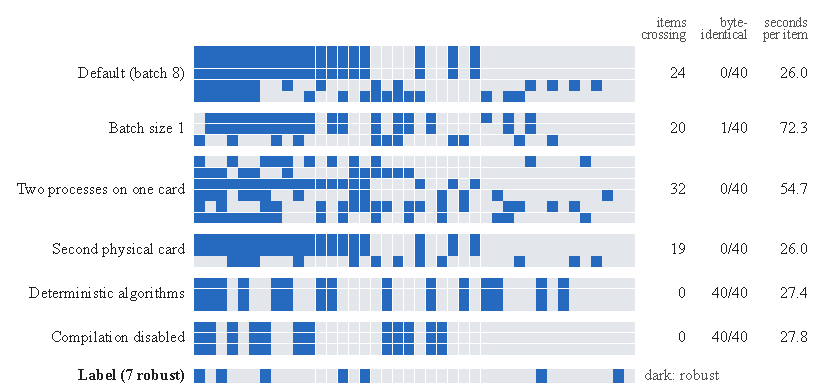
\includegraphics[width=\linewidth]{fig_rumore.pdf}
\caption{Predictions of the official pipeline for 40 preliminary public problems (columns) in 23 executions on DeepSeek (rows), by configuration; the last row is the label, dark cells are robust, and columns are sorted by how often they are predicted robust. At right: items whose prediction changes across the configuration's runs (more runs, more crossings), items whose generated text is byte-identical in all of them, and seconds per item.}
\label{fig:noise}
\end{figure}

\begin{table}[t]
\caption{Repeatability of the official pipeline on DeepSeek, 40 public problems, by configuration, in the order of Figure~\ref{fig:noise}. ``Crossings'': items whose prediction changes across the configuration's runs. ``Identical'': items whose generated text is byte-identical in all runs. Cost is runtime against the default configuration. Card 0 and card 1 are the two GPUs of the same machine. With two processes on one card, any five of its six runs give 29 to 31 crossings.}
\label{tab:reexec}
\centering
\small
\begin{tabular}{@{}lllllll@{}}
\toprule
\textbf{Configuration} & \textbf{Card} & \textbf{Runs} & \textbf{Crossings} & \textbf{Identical} & \textbf{Correct per run} & \textbf{Cost} \\
\midrule
Default (batch 8) & 0 & 5 & 24/40 & 0/40 & 24, 24, 24, 23, 24 & reference \\
Batch size 1 & 0 & 3 & 20/40 & 1/40 & 20, 21, 24 & +178\% \\
Two processes on one card & 0 & 6 & 32/40 & 0/40 & 24 to 28 & +110\% \\
Second physical card & 1 & 3 & 19/40 & 0/40 & 24, 24, 21 & +0\% \\
Deterministic algorithms & 0 & 3 & 0/40 & 40/40 & 24, 24, 24 & +5\% \\
Compilation disabled & 1 & 3 & 0/40 & 40/40 & 25, 25, 25 & +7\% \\
\bottomrule
\end{tabular}
\end{table}

\paragraph{Two candidate remedies.} Deterministic algorithms (PyTorch's, in warn-only mode, with deterministic cuDNN and a fixed cuBLAS workspace; Appendix~\ref{app:C}) and disabled compilation each made the generated text byte-identical in three sequential runs, at 5 to 7\% runtime cost. On card 0, the default configuration produced 24 crossings in five runs. Each remedy ran on one card where the default had produced crossings, each run in a new process, with no other process on that card. Three identical runs are weak evidence: the default configuration also gave three identical runs on card 0 before its fourth diverged, and five of its eight runs on the two cards shared one output. The two remedies produced different outputs, predicting 15 and 12 of the 40 problems robust, and because they ran on different cards we cannot tell whether the difference comes from the configuration or from the card. Neither gained more than one item (24 and 25 correct).

\paragraph{Distinct outputs.} The 23 executions fall into 14 distinct outputs, byte-identical within each. The same output appeared on both cards, and two runs launched in the same second on one card produced different outputs, so the output is not a property of the card alone; what selects it is not established. As only 7 of the 40 problems are robust and crossings largely cancel, accuracy moved much less than predictions: 21 to 24 correct in the default configuration on either card and 24 to 28 with two processes on one card, always below the 33 of the majority constant. An exploratory repetition of the official score extraction, whose third run ranks the 164 labeled problems at Spearman 0.24 against the first two, is in Appendix~\ref{app:C}.

\section{Regenerating the labels with our own protocol}\label{sec:labels}

\paragraph{Our labeling protocol.} We identified the organizers' perturbation families in the preliminary data (rephrase, rename, domain, distract, typos), regenerated them with gpt-oss-120b prompted with public examples, and gated each variant with gpt-oss-120b. An answer counts as correct when it matches gpt-oss-120b's answer on the original problem, because the preliminary data carry no answers; we did not check this key against the answers of the collections the problems come from. On the organizers' machine, with vLLM 0.28.0 [8] outside the official image, we labeled four models with two independent draws of variants (A and B, about 40 accepted variants per problem): 10 samples on the base problem and one per variant, at temperature 0.6, top-p 0.95 and at most 16,384 new tokens. Draw A's variants were also re-sampled with a new seed (A$'$). A label is robust when at least 6 of the 10 base samples are correct and every variant is answered correctly; unlike the earlier rule's conjunction, this requires the base problem to be solved.

A chain that reaches our cap is scored by the last boxed answer it contains, and counts as wrong without one; the organizers also count a response that reaches their limit without a parseable final answer as wrong [4]. Our protocol differs from the organizers' in perturbations, answer key, rule and sampling (one answer per variant, against 10 in the files behind most of their DeepSeek labels). Its decoding differs from the settings they publish, and its prompt may differ from the one behind their labels, which they have not stated.

\begin{table}[t]
\caption{Agreement of labels regenerated with our protocol: Cohen's kappa. The three columns for A and B treat variant chains that reached the 16,384-token cap in three ways: scored as in the protocol (by their last boxed answer, if any), dropped, or all counted as correct. The first of these columns and the A and A$'$ column give 95\% percentile bootstrap intervals over problems, and the script of Appendix~\ref{app:E} gives them for the other two. A problem has a label in a draw when it has at least one accepted variant (160 in A, 159 in B). Kappa between A and B uses the 159 problems labeled in both (150 for Qwen3.5-4B and 156 for DeepSeek when truncated chains are dropped), and between A and A$'$ 160. ``At cap'': percentage of variant chains that reached the cap in draws A and B. ``Robust'': percentage of problems labeled robust in draw A, as scored. The last column gives kappa of draw A with the organizers' preliminary DeepSeek labels: on the 138 published ones, and on the 160 that include 22 labels we derived (Section~\ref{sec:data}).}
\label{tab:label}
\centering
\small
\setlength{\tabcolsep}{3pt}
\begin{tabular}{@{}llllllll@{}}
\toprule
& & & \multicolumn{3}{l}{\textbf{A and B, truncated variant chains}} & & \\
\cmidrule(lr){4-6}
\textbf{Model} & \textbf{At cap} & \textbf{Robust} & \textbf{as scored} & \textbf{dropped} & \textbf{correct} & \textbf{A and A$'$} & \textbf{Organizers'} \\
\midrule
Skywork & 1.2, 1.5 & 74 & 0.44 [0.28, 0.59] & 0.39 & 0.39 & 0.79 [0.67, 0.89] & none \\
DeepSeek & 5.1, 6.1 & 39 & 0.41 [0.26, 0.55] & 0.35 & 0.36 & 0.46 [0.33, 0.59]$^{*}$ & 0.011; 0.025 \\
Olmo & 1.1, 0.9 & 68 & 0.38 [0.21, 0.54] & 0.39 & 0.39 & 0.65 [0.52, 0.78] & none \\
Qwen3.5-4B & 22.1, 29.2 & 9 & 0.18 [$-$0.06, 0.39] & 0.26 & 0.44 & not run & none \\
\bottomrule
\end{tabular}
\par\smallskip{\footnotesize $^{*}$On DeepSeek, A$'$ also received the answer-format line (end of this section), so this entry mixes seed and prompt.}
\end{table}

\paragraph{Results.} Under our protocol, two independent draws of variants give labels that agree at kappa 0.35 to 0.44 on Skywork, Olmo and DeepSeek, whether truncated variant chains are scored as in the protocol, dropped or all counted as correct (Table~\ref{tab:label}). On Qwen3.5-4B, 22 to 29\% of the variant chains reach the cap. Scoring these chains as in the protocol, dropping them or counting them all as correct gives agreement of 0.18, 0.26 and 0.44, and a robust share in draw A of 9\%, 83\% and 79\%. On Skywork, re-sampling the same variants with a new seed agrees far more than drawing new variants (0.79 against 0.44), so its label depends more on the variants than on the seed; on Olmo the gap is smaller (0.65 against 0.38), and on DeepSeek, where A$'$ also changed the prompt, it is 0.46 against 0.41.

Draw A's DeepSeek labels agree with the 138 labels the organizers published at kappa 0.011 [$-$0.13, 0.17], and with the 160 that include 22 of our derived labels at 0.025 [$-$0.12, 0.18]. Of the 36 problems with a published robust label, draw A calls 20 non-robust, and 4 of these change when truncated variants all count as correct. Of the 102 with a published non-robust label, draw A calls 44 robust. The reliability of the organizers' labels remains unmeasured. A retrospective calculation on the same saved answers with the main-phase threshold rule, applied as its pre-registration fixed it, with no filter on the base problem (Appendix~\ref{app:C}), gives test-retest point estimates between 0.34 and 0.56, below the pre-registered bar of 0.60, though three of the four intervals include it.

\paragraph{The prompt changes our labels.} In a first run with the bare problem text, later discarded, \mbox{Qwen3.5-4B} gave a final answer in the expected format in only 5 of its 1,640 base samples in draw A. With one instruction line requesting the format, 145 of 164 problems passed the base condition, against none. DeepSeek passed it on 147 of 164 with or without that line; its draws A and B ran without the line and A$'$ with it, and on the same variants its robust share moved from 39\% to 51\% of the 160 labeled problems, a change that mixes prompt and seed. Under our protocol, the label of Qwen3.5-4B therefore depends on the prompt. Whether this affects the organizers' labels is unknown: their baselines repository has a solve prompt that asks for an ANSWER line, but they have not said whether it was used for labeling (R3).

\section{The falsification campaign}\label{sec:campaign}

Table~\ref{tab:campaign} summarizes the campaign; Appendix~\ref{app:A} lists all 31 entries and explains three traps (rule T, the oracle H13, the duplicated pairs behind H2) and two pitfalls of the data. All entries use the preliminary data, except H16 to H18, which were scored on the 17 items of the warmup evaluation task.

\begin{table}[t]
\caption{The campaign in brief, in 19 of its 31 entries (Appendix~\ref{app:A} lists all). Ground truth is DeepSeek's and the preliminary pairs' unless stated; accuracy differences are in points against each pre-registration's baseline. H1, H7 and T count the 52 duplicated DeepSeek pairs twice; counted once, no verdict changes.}
\label{tab:campaign}
\centering
\small
\begin{tabular}{@{}L{5.5cm}L{1.9cm}L{5.6cm}@{}}
\toprule
\textbf{What we tested} & \textbf{Entries} & \textbf{Outcome} \\
\midrule
Text features; robustness as a property of the problem; labels, base accuracy and difficulty order across models & H1 to H5, H7 & rejected; H2 gained only when the duplicated pairs were counted twice \\
Official uncertainty features, logistic regression & H10 & 0.774 against a majority constant of 0.756, within the 0.692 $\pm$ 0.101 of the proposal [1] (method substituted) \\
Features cached for other models; per-target thresholds & H12, H13 & H12 rejected; the H13 ceiling withdrawn, $-$2.8 points when forced to rank \\
Our perturbation families, translation, self-consistency, the organizers' families regenerated (pilot), representation shift & H19, H22, H30 to H33 & rejected: kappa at most 0.02, AUROC at most 0.615 \\
Probes on DeepSeek's hidden states: ours and the organizers' published artifact & H36, H35 & survive their nulls; ours adds no detectable gain over length, and the artifact's score is probably in-sample \\
Trivial-robust rule, post hoc & T & a trap: +6.0 points on the preliminary pairs, +0.0 on \texttt{val-sample} \\
Identical bundles re-executed (warmup, 17 items) & H18 & noise confirmed: 11, 9, 11 and 11 correct \\
\bottomrule
\end{tabular}
\end{table}

\paragraph{Length and probes.} The character count of the problem alone orders the 164 DeepSeek labels at AUROC 0.704. Our logistic probe on DeepSeek's last-token hidden states, with layer and regularization chosen by inner cross-validation, reaches 0.710 out of fold with the original fold assignment. Over 20 other assignments, passed through the second-stage model below, it gives 0.57 to 0.76 (mean 0.69). Its scores correlate with length at Spearman +0.55, and residualized on log character count it gives 0.62. Its permutation null, rerun with 1{,}000 permutations of the whole nested procedure (the first version used 60, where 500 were pre-registered), gives $p = 0.002$. Restricted to the 138 published labels, these out-of-fold scores give 0.714 and length 0.733; retrained on those 138 alone with H36's procedure and seed, the probe gives 0.620. Combined with length in a second-stage model fitted on common outer folds, the probe changes AUROC over length alone by +0.005 on the 164 labels and by $-$0.010 on the 138 published ones (median bounds of the per-assignment 95\% intervals: $-$0.03 to 0.04, and $-$0.04 to 0.02): we detect no gain from adding the probe to length (Appendix~\ref{app:C}). This analysis replaces an earlier combination that leaked labels (Appendix~\ref{app:D}).

The organizers' published DeepSeek probe artifact orders the 164 DeepSeek labels at 0.739 with the aggregation we pre-registered and at 0.709 with its own, and at 0.62 and 0.57 residualized on log character count; its controls trained on shuffled labels give 0.68 at layer 31. The artifact does not record its training data; we infer that 137 of the 164 problems were among the public rows it was trained on, so these scores are probably largely in-sample. These length controls, which play the role of control tasks [7], were post hoc. Whether either probe reads anything beyond length that bears on robustness is not established. Apart from the three traps of Appendix~\ref{app:A}, no signal we scored by accuracy beats the majority constant by more than about one standard error on the preliminary labels, most of them DeepSeek's.

\section{Our entries}\label{sec:entries}

Our entry V8, pre-registered on 13 September, is the whole rule \texttt{return~[len(p)~>=~98 for~p~in~problems]}, with the threshold at the lower median of the 174 preliminary problems and the direction fixed on the preliminary pairs. On the original main-phase tasks it scored 11/21 and 10/19, like our entry v6 and the organizers' own entries. None of these beat the majority constant, which scores at least 11/21 and 10/19 on these tasks, and on so few items the ties do not show that length carries no signal (95\% Wilson intervals 0.32 to 0.72 and 0.32 to 0.73). On the 71 labeled rows of the official training set (revision of 17 September; 36 distinct problems), V8 differs from the all-robust constant on only 6 rows and is wrong on all 6 (46/71 against 52/71): too few to say what length is worth on official data. On the replacement tasks of 16 September, before and after the evaluation changed on 15 October [6], it predicted robust for every item (10/21 and 7/14), like an all-robust control. For the final test we nominated V8 (Codabench 1016713) and the constant (1016732), both on the Main track; our pre-registered predictions will be scored there (Appendix~\ref{app:B}).

\section{Recommendations}\label{sec:recs}

These rest mostly on DeepSeek and the preliminary data, and should be checked on the other models.
\begin{itemize}
\item \textbf{R1. Remove the variation between runs, and test the remedy:} on the same card with independent restarts, under load and across cards.
\item \textbf{R2. Repeat only where it decides something:} at the warmup's re-execution noise (a standard deviation of 1.0 item on 17, itself estimated from four runs), a one-item gap needs about eight runs per entry to reach two standard errors, so repeat only entries that run a model and sit near a prize boundary.
\item \textbf{R3. Say which prompt and decoding settings produced each released label file,} at least after the close.
\item \textbf{R4. Measure the label's reliability directly,} with two independent draws of variants labeled by the official process.
\item \textbf{R5. Show floors and noise on the leaderboard:} a row per constant predictor, the re-execution noise and binomial intervals.
\item \textbf{R6. Require a length control in white-box ablations.}
\item \textbf{R7. Remove the leaking field} \texttt{permutation\_type} from the aggregated datasets (Appendix~\ref{app:A}).
\end{itemize}

\paragraph{Code and data.} Our code, bundles, pre-registrations and outcome files are released at \href{https://github.com/Dan23RR/aimo-instrument}{\nolinkurl{github.com/Dan23RR/aimo-instrument}}. Its folder \texttt{reproduce/} recomputes the main tables from saved outputs and the six preliminary datasets, and the other numbers come from the dated records in \texttt{archive/} (Appendix~\ref{app:E}).

%%%%%% End of the main text: the six pages end here; the Limitations do not count %%%%%%
\label{fine-testo}

\section*{Limitations}

\begin{enumerate}[leftmargin=1.6em, itemsep=2pt, topsep=4pt, parsep=0pt]
\item \textbf{Preliminary data, not official data.} We did not repeat our label and probe analyses on the official training set, beyond the evaluation of V8 and a five-row check of our labels (Appendix~\ref{app:C}). Findings on label reliability and predictability may not generalize to the official evaluation setting.
\item \textbf{Our protocol, not the official one.} We did not regenerate labels with the organizers' published settings (100,000 tokens, temperature 1.0), with 10 answers per variant as in the files behind most DeepSeek labels, or on \texttt{train-main-v2}. The three treatments of truncated variant chains show how much our cap moves agreement between our draws; all three score base samples that reach the cap as the protocol does, and none of them reproduces longer decoding or a different temperature. Our low agreement with the organizers' labels is a fact about our process.
\item \textbf{One model.} We ran the probes, the re-execution study of Section~\ref{sec:reexec} and the comparisons of our regenerated labels with the organizers' preliminary labels only on DeepSeek.
\item \textbf{Re-execution.} We did not run the two candidate remedies on the same card, so card and configuration are confounded; we did not test either remedy under contention or on both cards, and we used 40 problems and one image.
\item \textbf{Records.} Some analyses rest on re-created scripts or dated records (Appendix~\ref{app:D}). Nothing here estimates performance on the final held-out problems.
\end{enumerate}

\section*{AI usage statement}

In this work, we used one generative AI tool, Claude (Anthropic), through Claude Code, for ideation, coding, analysis and writing. Ideation: it drafted the pre-registrations, including hypotheses, predictions and kill criteria, and searched and summarized the literature and the public records, including the organizers' Discord channels and the author's correspondence with them. Coding: it wrote the solution code of our bundles and the analysis and extraction scripts, ran them, and operated the organizers' virtual machine over SSH. Analysis: it computed and interpreted the results and ran automated adversarial reviews of hypotheses, drafts and code. Writing: it drafted the correspondence, this report and its revision after review.

It also made most of our Codabench uploads through the author's browser at the author's instruction. There were two exceptions: one resubmission (925822, 14 September), made without a specific instruction, and one submission that the author had not approved, sent in error and rejected before import (1016734, 28 October).

Language models were also components of our method: gpt-oss-120b generated and gated the perturbation variants and supplied the reference answers of Section~\ref{sec:labels}, and phi-4 translated problems for H22. The final decisions on the direction of the work, on the submissions (with the two exceptions above), on the nominations for the final test and on the claims of this report were the author's, and the author sent all correspondence personally. The author has reviewed all AI-assisted work and takes full responsibility for the final content of this report.

\begin{ack}
We thank Michal Štefánik, Róbert Belanec and the AIMO Interpretability team for the compute grant, a virtual machine with two GPUs, and for answering our questions; on 2 November they confirmed that the measurements taken on their machine may appear in this report. We also thank the three reviewers and the program chairs: two reviewers checked our analyses against the released code and data, and their checks corrected several of our claims. Other GPU time was rented on Modal and paid by the author or covered by Modal's platform credit. This work received no other funding, and the author has no competing interests.
\end{ack}

\section*{References}
{\small
[1] M. Štefánik, P. Mondorf, A. Waldis, Q. Liu, C. Yang, M. Spiegel, J. Kuchař, M. Kadlčík, A. Vawda-Oomerjee, C. Liu, S. Frieder, B. Plank, F. Barez and P. Stenetorp. AIMO Interpretability Challenge. CoRR, abs/2607.13899, 2026. doi:10.48550/arXiv.2607.13899.

[2] H. He and Thinking Machines Lab. Defeating Nondeterminism in LLM Inference. Thinking Machines Lab: Connectionism, 2025.

[3] J. Yuan, H. Li, X. Ding, W. Xie, Y.-J. Li, W. Zhao, K. Wan, J. Shi, X. Hu and Z. Liu. Understanding and Mitigating Numerical Sources of Nondeterminism in LLM Inference. NeurIPS 2025. arXiv:2506.09501.

[4] AIMO Interpretability Challenge website and FAQ. \url{https://aimo-interp.github.io} (accessed 28 October 2026), and its source repository aimo-interp/aimo-interp.github.io on GitHub.

[5] aimo-interp/getting-started and aimo-interp/baselines, GitHub repositories: README and issues \#6 and \#10 of getting-started; aimo-interp datasets on Hugging Face, including \texttt{train-main-v2} and \texttt{val-sample}.

[6] AIMO Interpretability Challenge Discord, \#announcements and \#qa: 5, 15 and 22 September, 9, 15, 16 and 20 October 2026.

[7] J. Hewitt and P. Liang. Designing and Interpreting Probes with Control Tasks. EMNLP-IJCNLP 2019.

[8] W. Kwon et al. Efficient Memory Management for Large Language Model Serving with PagedAttention. SOSP 2023.

[9] D. Hendrycks et al. Measuring Mathematical Problem Solving With the MATH Dataset. NeurIPS 2021 Datasets and Benchmarks Track. arXiv:2103.03874.
}

%%%%%% End of the references %%%%%%
\clearpage
\appendix
\raggedright

\input{app_A}
\input{app_B}
\input{app_C}
\input{app_D}
\input{app_E}

\newpage
\input{checklist_compilata.tex}

\end{document}
".
%% Every line numbered (same numbering, used to find the lines cited in the note): "\def\everyline{}\documentclass{article}

%% Conditional revision of November 2026: six pages of main text, from the title to the end of Section 7 (label
%% fine-testo); the Limitations, the AI usage statement, the references and the appendices do not count.
%% Final mode with the workshop name. Line numbers on every fifth line, small and grey, for the note to the
%% program chairs, who asked for section and line numbers. Copy without them: pdflatex "\def\cleancopy{}\input{main}".
%% Every line numbered (same numbering, used to find the lines cited in the note): "\def\everyline{}\input{main}".
\usepackage[final,sglblindworkshop]{neurips_2026}
\workshoptitle{AIMO Interpretability Challenge}
\ifdefined\cleancopy\else
  \usepackage{lineno}
  \linenumbers
  \ifdefined\everyline\else\modulolinenumbers[5]\fi
  \renewcommand\linenumberfont{\normalfont\tiny\sffamily\color{black!45}}
\fi

\usepackage[utf8]{inputenc}
\usepackage[T1]{fontenc}
%% Typewriter text in Latin Modern, the Type 1 version of the default Computer Modern typewriter, with the same
%% widths: without it, \texttt in T1 encoding becomes bitmap (Type 3) fonts, and the template asks for Type 1 fonts.
\renewcommand{\ttdefault}{lmtt}
\usepackage{hyperref}
\hypersetup{pdftitle={The Instrument Behind the Leaderboard: Re-Execution Noise and Label Regeneration in the AIMO Interpretability Challenge}, pdfauthor={Daniel Culotta}}
\usepackage{url}
\def\UrlBreaks{\do\/\do\.\do\_\do\-\do\:}
\usepackage{booktabs}
\usepackage{array}
\usepackage{longtable}
\newcolumntype{L}[1]{>{\raggedright\arraybackslash}p{#1}}
\usepackage{amsfonts}
\usepackage{microtype}
\usepackage{xcolor}
\usepackage{graphicx}
\usepackage{enumitem}
\usepackage{needspace}
\setlist[itemize]{leftmargin=1.4em, itemsep=2pt, topsep=4pt, parsep=0pt}
\setlist[itemize,2]{label=$\circ$}
\renewcommand{\arraystretch}{1.15}
\raggedbottom

\title{The Instrument Behind the Leaderboard: Re-Execution Noise and Label Regeneration in the AIMO Interpretability Challenge}

\author{%
  Daniel Culotta \\
  Independent researcher
}

\begin{document}

\maketitle

\begin{abstract}
We treat the AIMO Interpretability benchmark, which asks whether a model's answer to a math problem survives perturbations, as a measurement instrument. Almost all our label and probe analyses use the preliminary datasets. As the program chairs note, these differ from the official training and validation data in sampling, perturbations and eligibility, so findings on label reliability and predictability may not hold in the official evaluation. First, on DeepSeek-R1-0528-Qwen3-8B in the official pipeline, 24 of 40 items changed prediction across five default runs. Turning compilation off, or deterministic algorithms on, gave three byte-identical runs, each on one card. Second, we regenerated labels with our own protocol, not the official one: our perturbations and answer key, one answer per variant, a 16,384-token cap and temperature 0.6, where the organizers publish 100,000 tokens and 1.0. Two independent draws agree at kappa 0.35 to 0.44 on three of four models however truncated chains are treated, and 0.18 to 0.44 on Qwen3.5-4B, whose chains often reach the cap. Draw A agrees with the 138 published DeepSeek labels at kappa 0.01. This describes our protocol and does not measure the reliability of the organizers' labels. Third, of the 27 dated hypotheses with a kill criterion, 21 failed it. Our probe on DeepSeek's hidden states does no better than problem length (AUROC 0.710 against 0.704; below length on the published labels) and adds nothing detectable to it.
\end{abstract}

\section{Introduction}\label{sec:1}

A leaderboard is a measurement. Its score is read off an instrument made of a label, an evaluation set, an inference pipeline and the hardware it runs on. When the label is itself produced by a stochastic process, the instrument has noise of its own, which a single submission cannot see. We measure the re-execution noise of the official extraction and regressor, and the repeatability of labels regenerated with our own protocol, not the noise of the organizers' labels.

We study the instrument of the AIMO Interpretability Challenge, in which a submission predicts, for a given model and math problem, whether the model's answer is robust to perturbations of the problem [1]. We ran our work as a falsification campaign: every hypothesis was recorded in a dated file, 26 of the 31 before their data were seen, and every tested hypothesis is reported. Of the 31 entries, 27 carried a kill criterion written before their test ran (for 3 of them in a written plan rather than a frozen pre-registration, and for H2 after its concordance had been seen). By that criterion 21 were rejected, 5 survived and 1 is not established (Appendix~\ref{app:A}).

\paragraph{Scope.} Three limits apply.
\begin{itemize}
\item \textbf{Preliminary and official data.} Almost all of our label and probe analyses use the six preliminary public datasets released before the main phase. Their labels follow an earlier rule than those of the official training set (\texttt{train-main-v2}) and of the validation and test tasks [5]; as the program chairs noted in their meta-review, their sampling procedures, perturbations and eligibility criteria also differ. Beyond the label rule, we did not compare the two. Unless we say otherwise, a result on labels or on their predictability holds for the preliminary data and may not hold in the official evaluation setting.
\item \textbf{Our labeling protocol is not the official one.} When we regenerate labels (Section~\ref{sec:labels}), we use our own perturbations, prompts, sampling, decoding, answer key and labeling rule. Disagreement with the organizers' preliminary labels therefore shows that the two processes give different labels; it does not establish that their labels are unreliable or irreproducible.
\item \textbf{Mostly one model.} The re-execution study of Section~\ref{sec:reexec}, the probe analyses and every comparison of our regenerated labels with the organizers' preliminary labels are on DeepSeek-R1-0528-Qwen3-8B. Regenerated labels cover four models, but no conclusion about the official benchmark is established across models.
\end{itemize}

Within these limits, Sections~\ref{sec:reexec} to~\ref{sec:campaign} report re-execution noise and two candidate remedies, our regenerated labels, and signals that do no better than problem length or come from an artifact of the data. Nondeterminism of LLM inference is documented in general [2, 3]; we add its size for one model, one submission and 40 problems on this benchmark's hardware and pipeline. We make no claim about any participant's method.

\section{The task, the labels and the data}\label{sec:data}

\paragraph{Task.} A submission receives a model identifier, a reasoning effort and a list of problems, and returns one robustness verdict per problem, offline on one GPU within one hour [4, 5], or 70 minutes since 15 October [6]. The models are Qwen3.5-4B, Skywork-OR1-Math-7B, Olmo-3-7B-Think and \mbox{DeepSeek-R1-0528-Qwen3-8B} in both tracks, and gpt-oss-120b in the Main track only.

\paragraph{Official data.} The main-phase training set \texttt{train-main-v2} labels all five models with a threshold on the largest accuracy drop across perturbation families: robust at most 0.10, non-robust at least 0.25, no label in between [5]. The organizers' published decoding settings are up to 100,000 tokens at temperature 1.0, top-k 40 and top-p 0.95, and a response that reaches the limit without a final answer counts as wrong [4]. Since 16 September the private validation tasks have 21 items (Main) and 14 (Small), on which the binomial standard error of an accuracy near one half is 10.9 and 13.4 points; the final test uses 30 to 50 new problems [5, 6].

\paragraph{Preliminary data.} Six datasets released before the main phase aggregate to 335 (model, problem) pairs over 174 distinct problems, up to eight per problem; 52 pairs repeat the DeepSeek measurements under a second model name. Their labels follow an earlier rule: on all 379 labeled rows (a pair can have several), the label equals the conjunction ``no perturbation lowered accuracy''. A per-family majority rule (``more than half of the answers are correct in every perturbation family'') reproduces the same 379 labels, so these rows cannot tell the two rules apart. Whether they used the decoding settings above is not documented; in the files behind most DeepSeek labels, most variants listed as lowering accuracy were answered 10 times. We call their labels the organizers' preliminary labels, and keep ``official'' for \texttt{train-main-v2} and the validation and test tasks.

\paragraph{DeepSeek labels.} DeepSeek is the only evaluated model with many preliminary labels: 164 distinct problems (the 52 duplicated pairs count once). For 138 of them the data publish a label. For the other 26 we derived one with the conjunction, which makes 4 of them robust; the majority rule would make 21 robust, so these 26 labels depend on the choice of rule. We therefore report results on the 138 published labels separately.

\section{Re-execution noise on the evaluation workers' type of GPU}\label{sec:reexec}

On a virtual machine lent by the organizers, with two NVIDIA RTX PRO 6000 Blackwell Server Edition GPUs (the type the evaluation workers use), we ran 40 preliminary public problems through the official runtime image, extraction and regressor, unmodified, on DeepSeek. Decoding was greedy, with at most 4,096 new tokens in batches of 8. The 40 labels are DeepSeek's of Section~\ref{sec:data}: 28 published and 12 that we derived with the conjunction, which include 3 of the 7 robust ones. Figure~\ref{fig:noise} shows the 23 executions; Table~\ref{tab:reexec} gives the repeatability of each configuration.

\begin{figure}[t]
\centering
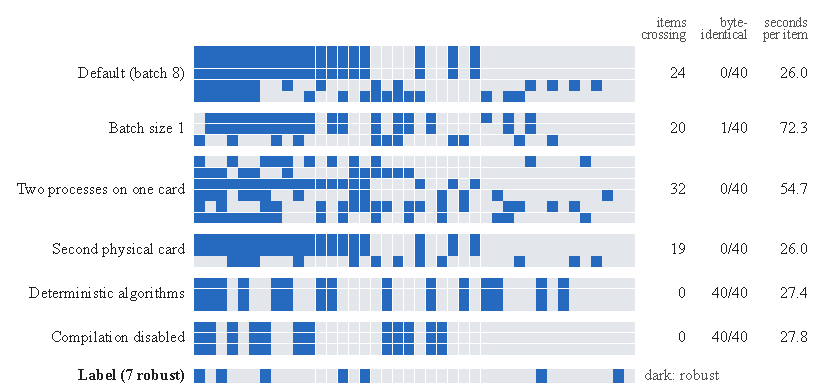
\includegraphics[width=\linewidth]{fig_rumore.pdf}
\caption{Predictions of the official pipeline for 40 preliminary public problems (columns) in 23 executions on DeepSeek (rows), by configuration; the last row is the label, dark cells are robust, and columns are sorted by how often they are predicted robust. At right: items whose prediction changes across the configuration's runs (more runs, more crossings), items whose generated text is byte-identical in all of them, and seconds per item.}
\label{fig:noise}
\end{figure}

\begin{table}[t]
\caption{Repeatability of the official pipeline on DeepSeek, 40 public problems, by configuration, in the order of Figure~\ref{fig:noise}. ``Crossings'': items whose prediction changes across the configuration's runs. ``Identical'': items whose generated text is byte-identical in all runs. Cost is runtime against the default configuration. Card 0 and card 1 are the two GPUs of the same machine. With two processes on one card, any five of its six runs give 29 to 31 crossings.}
\label{tab:reexec}
\centering
\small
\begin{tabular}{@{}lllllll@{}}
\toprule
\textbf{Configuration} & \textbf{Card} & \textbf{Runs} & \textbf{Crossings} & \textbf{Identical} & \textbf{Correct per run} & \textbf{Cost} \\
\midrule
Default (batch 8) & 0 & 5 & 24/40 & 0/40 & 24, 24, 24, 23, 24 & reference \\
Batch size 1 & 0 & 3 & 20/40 & 1/40 & 20, 21, 24 & +178\% \\
Two processes on one card & 0 & 6 & 32/40 & 0/40 & 24 to 28 & +110\% \\
Second physical card & 1 & 3 & 19/40 & 0/40 & 24, 24, 21 & +0\% \\
Deterministic algorithms & 0 & 3 & 0/40 & 40/40 & 24, 24, 24 & +5\% \\
Compilation disabled & 1 & 3 & 0/40 & 40/40 & 25, 25, 25 & +7\% \\
\bottomrule
\end{tabular}
\end{table}

\paragraph{Two candidate remedies.} Deterministic algorithms (PyTorch's, in warn-only mode, with deterministic cuDNN and a fixed cuBLAS workspace; Appendix~\ref{app:C}) and disabled compilation each made the generated text byte-identical in three sequential runs, at 5 to 7\% runtime cost. On card 0, the default configuration produced 24 crossings in five runs. Each remedy ran on one card where the default had produced crossings, each run in a new process, with no other process on that card. Three identical runs are weak evidence: the default configuration also gave three identical runs on card 0 before its fourth diverged, and five of its eight runs on the two cards shared one output. The two remedies produced different outputs, predicting 15 and 12 of the 40 problems robust, and because they ran on different cards we cannot tell whether the difference comes from the configuration or from the card. Neither gained more than one item (24 and 25 correct).

\paragraph{Distinct outputs.} The 23 executions fall into 14 distinct outputs, byte-identical within each. The same output appeared on both cards, and two runs launched in the same second on one card produced different outputs, so the output is not a property of the card alone; what selects it is not established. As only 7 of the 40 problems are robust and crossings largely cancel, accuracy moved much less than predictions: 21 to 24 correct in the default configuration on either card and 24 to 28 with two processes on one card, always below the 33 of the majority constant. An exploratory repetition of the official score extraction, whose third run ranks the 164 labeled problems at Spearman 0.24 against the first two, is in Appendix~\ref{app:C}.

\section{Regenerating the labels with our own protocol}\label{sec:labels}

\paragraph{Our labeling protocol.} We identified the organizers' perturbation families in the preliminary data (rephrase, rename, domain, distract, typos), regenerated them with gpt-oss-120b prompted with public examples, and gated each variant with gpt-oss-120b. An answer counts as correct when it matches gpt-oss-120b's answer on the original problem, because the preliminary data carry no answers; we did not check this key against the answers of the collections the problems come from. On the organizers' machine, with vLLM 0.28.0 [8] outside the official image, we labeled four models with two independent draws of variants (A and B, about 40 accepted variants per problem): 10 samples on the base problem and one per variant, at temperature 0.6, top-p 0.95 and at most 16,384 new tokens. Draw A's variants were also re-sampled with a new seed (A$'$). A label is robust when at least 6 of the 10 base samples are correct and every variant is answered correctly; unlike the earlier rule's conjunction, this requires the base problem to be solved.

A chain that reaches our cap is scored by the last boxed answer it contains, and counts as wrong without one; the organizers also count a response that reaches their limit without a parseable final answer as wrong [4]. Our protocol differs from the organizers' in perturbations, answer key, rule and sampling (one answer per variant, against 10 in the files behind most of their DeepSeek labels). Its decoding differs from the settings they publish, and its prompt may differ from the one behind their labels, which they have not stated.

\begin{table}[t]
\caption{Agreement of labels regenerated with our protocol: Cohen's kappa. The three columns for A and B treat variant chains that reached the 16,384-token cap in three ways: scored as in the protocol (by their last boxed answer, if any), dropped, or all counted as correct. The first of these columns and the A and A$'$ column give 95\% percentile bootstrap intervals over problems, and the script of Appendix~\ref{app:E} gives them for the other two. A problem has a label in a draw when it has at least one accepted variant (160 in A, 159 in B). Kappa between A and B uses the 159 problems labeled in both (150 for Qwen3.5-4B and 156 for DeepSeek when truncated chains are dropped), and between A and A$'$ 160. ``At cap'': percentage of variant chains that reached the cap in draws A and B. ``Robust'': percentage of problems labeled robust in draw A, as scored. The last column gives kappa of draw A with the organizers' preliminary DeepSeek labels: on the 138 published ones, and on the 160 that include 22 labels we derived (Section~\ref{sec:data}).}
\label{tab:label}
\centering
\small
\setlength{\tabcolsep}{3pt}
\begin{tabular}{@{}llllllll@{}}
\toprule
& & & \multicolumn{3}{l}{\textbf{A and B, truncated variant chains}} & & \\
\cmidrule(lr){4-6}
\textbf{Model} & \textbf{At cap} & \textbf{Robust} & \textbf{as scored} & \textbf{dropped} & \textbf{correct} & \textbf{A and A$'$} & \textbf{Organizers'} \\
\midrule
Skywork & 1.2, 1.5 & 74 & 0.44 [0.28, 0.59] & 0.39 & 0.39 & 0.79 [0.67, 0.89] & none \\
DeepSeek & 5.1, 6.1 & 39 & 0.41 [0.26, 0.55] & 0.35 & 0.36 & 0.46 [0.33, 0.59]$^{*}$ & 0.011; 0.025 \\
Olmo & 1.1, 0.9 & 68 & 0.38 [0.21, 0.54] & 0.39 & 0.39 & 0.65 [0.52, 0.78] & none \\
Qwen3.5-4B & 22.1, 29.2 & 9 & 0.18 [$-$0.06, 0.39] & 0.26 & 0.44 & not run & none \\
\bottomrule
\end{tabular}
\par\smallskip{\footnotesize $^{*}$On DeepSeek, A$'$ also received the answer-format line (end of this section), so this entry mixes seed and prompt.}
\end{table}

\paragraph{Results.} Under our protocol, two independent draws of variants give labels that agree at kappa 0.35 to 0.44 on Skywork, Olmo and DeepSeek, whether truncated variant chains are scored as in the protocol, dropped or all counted as correct (Table~\ref{tab:label}). On Qwen3.5-4B, 22 to 29\% of the variant chains reach the cap. Scoring these chains as in the protocol, dropping them or counting them all as correct gives agreement of 0.18, 0.26 and 0.44, and a robust share in draw A of 9\%, 83\% and 79\%. On Skywork, re-sampling the same variants with a new seed agrees far more than drawing new variants (0.79 against 0.44), so its label depends more on the variants than on the seed; on Olmo the gap is smaller (0.65 against 0.38), and on DeepSeek, where A$'$ also changed the prompt, it is 0.46 against 0.41.

Draw A's DeepSeek labels agree with the 138 labels the organizers published at kappa 0.011 [$-$0.13, 0.17], and with the 160 that include 22 of our derived labels at 0.025 [$-$0.12, 0.18]. Of the 36 problems with a published robust label, draw A calls 20 non-robust, and 4 of these change when truncated variants all count as correct. Of the 102 with a published non-robust label, draw A calls 44 robust. The reliability of the organizers' labels remains unmeasured. A retrospective calculation on the same saved answers with the main-phase threshold rule, applied as its pre-registration fixed it, with no filter on the base problem (Appendix~\ref{app:C}), gives test-retest point estimates between 0.34 and 0.56, below the pre-registered bar of 0.60, though three of the four intervals include it.

\paragraph{The prompt changes our labels.} In a first run with the bare problem text, later discarded, \mbox{Qwen3.5-4B} gave a final answer in the expected format in only 5 of its 1,640 base samples in draw A. With one instruction line requesting the format, 145 of 164 problems passed the base condition, against none. DeepSeek passed it on 147 of 164 with or without that line; its draws A and B ran without the line and A$'$ with it, and on the same variants its robust share moved from 39\% to 51\% of the 160 labeled problems, a change that mixes prompt and seed. Under our protocol, the label of Qwen3.5-4B therefore depends on the prompt. Whether this affects the organizers' labels is unknown: their baselines repository has a solve prompt that asks for an ANSWER line, but they have not said whether it was used for labeling (R3).

\section{The falsification campaign}\label{sec:campaign}

Table~\ref{tab:campaign} summarizes the campaign; Appendix~\ref{app:A} lists all 31 entries and explains three traps (rule T, the oracle H13, the duplicated pairs behind H2) and two pitfalls of the data. All entries use the preliminary data, except H16 to H18, which were scored on the 17 items of the warmup evaluation task.

\begin{table}[t]
\caption{The campaign in brief, in 19 of its 31 entries (Appendix~\ref{app:A} lists all). Ground truth is DeepSeek's and the preliminary pairs' unless stated; accuracy differences are in points against each pre-registration's baseline. H1, H7 and T count the 52 duplicated DeepSeek pairs twice; counted once, no verdict changes.}
\label{tab:campaign}
\centering
\small
\begin{tabular}{@{}L{5.5cm}L{1.9cm}L{5.6cm}@{}}
\toprule
\textbf{What we tested} & \textbf{Entries} & \textbf{Outcome} \\
\midrule
Text features; robustness as a property of the problem; labels, base accuracy and difficulty order across models & H1 to H5, H7 & rejected; H2 gained only when the duplicated pairs were counted twice \\
Official uncertainty features, logistic regression & H10 & 0.774 against a majority constant of 0.756, within the 0.692 $\pm$ 0.101 of the proposal [1] (method substituted) \\
Features cached for other models; per-target thresholds & H12, H13 & H12 rejected; the H13 ceiling withdrawn, $-$2.8 points when forced to rank \\
Our perturbation families, translation, self-consistency, the organizers' families regenerated (pilot), representation shift & H19, H22, H30 to H33 & rejected: kappa at most 0.02, AUROC at most 0.615 \\
Probes on DeepSeek's hidden states: ours and the organizers' published artifact & H36, H35 & survive their nulls; ours adds no detectable gain over length, and the artifact's score is probably in-sample \\
Trivial-robust rule, post hoc & T & a trap: +6.0 points on the preliminary pairs, +0.0 on \texttt{val-sample} \\
Identical bundles re-executed (warmup, 17 items) & H18 & noise confirmed: 11, 9, 11 and 11 correct \\
\bottomrule
\end{tabular}
\end{table}

\paragraph{Length and probes.} The character count of the problem alone orders the 164 DeepSeek labels at AUROC 0.704. Our logistic probe on DeepSeek's last-token hidden states, with layer and regularization chosen by inner cross-validation, reaches 0.710 out of fold with the original fold assignment. Over 20 other assignments, passed through the second-stage model below, it gives 0.57 to 0.76 (mean 0.69). Its scores correlate with length at Spearman +0.55, and residualized on log character count it gives 0.62. Its permutation null, rerun with 1{,}000 permutations of the whole nested procedure (the first version used 60, where 500 were pre-registered), gives $p = 0.002$. Restricted to the 138 published labels, these out-of-fold scores give 0.714 and length 0.733; retrained on those 138 alone with H36's procedure and seed, the probe gives 0.620. Combined with length in a second-stage model fitted on common outer folds, the probe changes AUROC over length alone by +0.005 on the 164 labels and by $-$0.010 on the 138 published ones (median bounds of the per-assignment 95\% intervals: $-$0.03 to 0.04, and $-$0.04 to 0.02): we detect no gain from adding the probe to length (Appendix~\ref{app:C}). This analysis replaces an earlier combination that leaked labels (Appendix~\ref{app:D}).

The organizers' published DeepSeek probe artifact orders the 164 DeepSeek labels at 0.739 with the aggregation we pre-registered and at 0.709 with its own, and at 0.62 and 0.57 residualized on log character count; its controls trained on shuffled labels give 0.68 at layer 31. The artifact does not record its training data; we infer that 137 of the 164 problems were among the public rows it was trained on, so these scores are probably largely in-sample. These length controls, which play the role of control tasks [7], were post hoc. Whether either probe reads anything beyond length that bears on robustness is not established. Apart from the three traps of Appendix~\ref{app:A}, no signal we scored by accuracy beats the majority constant by more than about one standard error on the preliminary labels, most of them DeepSeek's.

\section{Our entries}\label{sec:entries}

Our entry V8, pre-registered on 13 September, is the whole rule \texttt{return~[len(p)~>=~98 for~p~in~problems]}, with the threshold at the lower median of the 174 preliminary problems and the direction fixed on the preliminary pairs. On the original main-phase tasks it scored 11/21 and 10/19, like our entry v6 and the organizers' own entries. None of these beat the majority constant, which scores at least 11/21 and 10/19 on these tasks, and on so few items the ties do not show that length carries no signal (95\% Wilson intervals 0.32 to 0.72 and 0.32 to 0.73). On the 71 labeled rows of the official training set (revision of 17 September; 36 distinct problems), V8 differs from the all-robust constant on only 6 rows and is wrong on all 6 (46/71 against 52/71): too few to say what length is worth on official data. On the replacement tasks of 16 September, before and after the evaluation changed on 15 October [6], it predicted robust for every item (10/21 and 7/14), like an all-robust control. For the final test we nominated V8 (Codabench 1016713) and the constant (1016732), both on the Main track; our pre-registered predictions will be scored there (Appendix~\ref{app:B}).

\section{Recommendations}\label{sec:recs}

These rest mostly on DeepSeek and the preliminary data, and should be checked on the other models.
\begin{itemize}
\item \textbf{R1. Remove the variation between runs, and test the remedy:} on the same card with independent restarts, under load and across cards.
\item \textbf{R2. Repeat only where it decides something:} at the warmup's re-execution noise (a standard deviation of 1.0 item on 17, itself estimated from four runs), a one-item gap needs about eight runs per entry to reach two standard errors, so repeat only entries that run a model and sit near a prize boundary.
\item \textbf{R3. Say which prompt and decoding settings produced each released label file,} at least after the close.
\item \textbf{R4. Measure the label's reliability directly,} with two independent draws of variants labeled by the official process.
\item \textbf{R5. Show floors and noise on the leaderboard:} a row per constant predictor, the re-execution noise and binomial intervals.
\item \textbf{R6. Require a length control in white-box ablations.}
\item \textbf{R7. Remove the leaking field} \texttt{permutation\_type} from the aggregated datasets (Appendix~\ref{app:A}).
\end{itemize}

\paragraph{Code and data.} Our code, bundles, pre-registrations and outcome files are released at \href{https://github.com/Dan23RR/aimo-instrument}{\nolinkurl{github.com/Dan23RR/aimo-instrument}}. Its folder \texttt{reproduce/} recomputes the main tables from saved outputs and the six preliminary datasets, and the other numbers come from the dated records in \texttt{archive/} (Appendix~\ref{app:E}).

%%%%%% End of the main text: the six pages end here; the Limitations do not count %%%%%%
\label{fine-testo}

\section*{Limitations}

\begin{enumerate}[leftmargin=1.6em, itemsep=2pt, topsep=4pt, parsep=0pt]
\item \textbf{Preliminary data, not official data.} We did not repeat our label and probe analyses on the official training set, beyond the evaluation of V8 and a five-row check of our labels (Appendix~\ref{app:C}). Findings on label reliability and predictability may not generalize to the official evaluation setting.
\item \textbf{Our protocol, not the official one.} We did not regenerate labels with the organizers' published settings (100,000 tokens, temperature 1.0), with 10 answers per variant as in the files behind most DeepSeek labels, or on \texttt{train-main-v2}. The three treatments of truncated variant chains show how much our cap moves agreement between our draws; all three score base samples that reach the cap as the protocol does, and none of them reproduces longer decoding or a different temperature. Our low agreement with the organizers' labels is a fact about our process.
\item \textbf{One model.} We ran the probes, the re-execution study of Section~\ref{sec:reexec} and the comparisons of our regenerated labels with the organizers' preliminary labels only on DeepSeek.
\item \textbf{Re-execution.} We did not run the two candidate remedies on the same card, so card and configuration are confounded; we did not test either remedy under contention or on both cards, and we used 40 problems and one image.
\item \textbf{Records.} Some analyses rest on re-created scripts or dated records (Appendix~\ref{app:D}). Nothing here estimates performance on the final held-out problems.
\end{enumerate}

\section*{AI usage statement}

In this work, we used one generative AI tool, Claude (Anthropic), through Claude Code, for ideation, coding, analysis and writing. Ideation: it drafted the pre-registrations, including hypotheses, predictions and kill criteria, and searched and summarized the literature and the public records, including the organizers' Discord channels and the author's correspondence with them. Coding: it wrote the solution code of our bundles and the analysis and extraction scripts, ran them, and operated the organizers' virtual machine over SSH. Analysis: it computed and interpreted the results and ran automated adversarial reviews of hypotheses, drafts and code. Writing: it drafted the correspondence, this report and its revision after review.

It also made most of our Codabench uploads through the author's browser at the author's instruction. There were two exceptions: one resubmission (925822, 14 September), made without a specific instruction, and one submission that the author had not approved, sent in error and rejected before import (1016734, 28 October).

Language models were also components of our method: gpt-oss-120b generated and gated the perturbation variants and supplied the reference answers of Section~\ref{sec:labels}, and phi-4 translated problems for H22. The final decisions on the direction of the work, on the submissions (with the two exceptions above), on the nominations for the final test and on the claims of this report were the author's, and the author sent all correspondence personally. The author has reviewed all AI-assisted work and takes full responsibility for the final content of this report.

\begin{ack}
We thank Michal Štefánik, Róbert Belanec and the AIMO Interpretability team for the compute grant, a virtual machine with two GPUs, and for answering our questions; on 2 November they confirmed that the measurements taken on their machine may appear in this report. We also thank the three reviewers and the program chairs: two reviewers checked our analyses against the released code and data, and their checks corrected several of our claims. Other GPU time was rented on Modal and paid by the author or covered by Modal's platform credit. This work received no other funding, and the author has no competing interests.
\end{ack}

\section*{References}
{\small
[1] M. Štefánik, P. Mondorf, A. Waldis, Q. Liu, C. Yang, M. Spiegel, J. Kuchař, M. Kadlčík, A. Vawda-Oomerjee, C. Liu, S. Frieder, B. Plank, F. Barez and P. Stenetorp. AIMO Interpretability Challenge. CoRR, abs/2607.13899, 2026. doi:10.48550/arXiv.2607.13899.

[2] H. He and Thinking Machines Lab. Defeating Nondeterminism in LLM Inference. Thinking Machines Lab: Connectionism, 2025.

[3] J. Yuan, H. Li, X. Ding, W. Xie, Y.-J. Li, W. Zhao, K. Wan, J. Shi, X. Hu and Z. Liu. Understanding and Mitigating Numerical Sources of Nondeterminism in LLM Inference. NeurIPS 2025. arXiv:2506.09501.

[4] AIMO Interpretability Challenge website and FAQ. \url{https://aimo-interp.github.io} (accessed 28 October 2026), and its source repository aimo-interp/aimo-interp.github.io on GitHub.

[5] aimo-interp/getting-started and aimo-interp/baselines, GitHub repositories: README and issues \#6 and \#10 of getting-started; aimo-interp datasets on Hugging Face, including \texttt{train-main-v2} and \texttt{val-sample}.

[6] AIMO Interpretability Challenge Discord, \#announcements and \#qa: 5, 15 and 22 September, 9, 15, 16 and 20 October 2026.

[7] J. Hewitt and P. Liang. Designing and Interpreting Probes with Control Tasks. EMNLP-IJCNLP 2019.

[8] W. Kwon et al. Efficient Memory Management for Large Language Model Serving with PagedAttention. SOSP 2023.

[9] D. Hendrycks et al. Measuring Mathematical Problem Solving With the MATH Dataset. NeurIPS 2021 Datasets and Benchmarks Track. arXiv:2103.03874.
}

%%%%%% End of the references %%%%%%
\clearpage
\appendix
\raggedright

\input{app_A}
\input{app_B}
\input{app_C}
\input{app_D}
\input{app_E}

\newpage
\input{checklist_compilata.tex}

\end{document}
".
\usepackage[final,sglblindworkshop]{neurips_2026}
\workshoptitle{AIMO Interpretability Challenge}
\ifdefined\cleancopy\else
  \usepackage{lineno}
  \linenumbers
  \ifdefined\everyline\else\modulolinenumbers[5]\fi
  \renewcommand\linenumberfont{\normalfont\tiny\sffamily\color{black!45}}
\fi

\usepackage[utf8]{inputenc}
\usepackage[T1]{fontenc}
%% Typewriter text in Latin Modern, the Type 1 version of the default Computer Modern typewriter, with the same
%% widths: without it, \texttt in T1 encoding becomes bitmap (Type 3) fonts, and the template asks for Type 1 fonts.
\renewcommand{\ttdefault}{lmtt}
\usepackage{hyperref}
\hypersetup{pdftitle={The Instrument Behind the Leaderboard: Re-Execution Noise and Label Regeneration in the AIMO Interpretability Challenge}, pdfauthor={Daniel Culotta}}
\usepackage{url}
\def\UrlBreaks{\do\/\do\.\do\_\do\-\do\:}
\usepackage{booktabs}
\usepackage{array}
\usepackage{longtable}
\newcolumntype{L}[1]{>{\raggedright\arraybackslash}p{#1}}
\usepackage{amsfonts}
\usepackage{microtype}
\usepackage{xcolor}
\usepackage{graphicx}
\usepackage{enumitem}
\usepackage{needspace}
\setlist[itemize]{leftmargin=1.4em, itemsep=2pt, topsep=4pt, parsep=0pt}
\setlist[itemize,2]{label=$\circ$}
\renewcommand{\arraystretch}{1.15}
\raggedbottom

\title{The Instrument Behind the Leaderboard: Re-Execution Noise and Label Regeneration in the AIMO Interpretability Challenge}

\author{%
  Daniel Culotta \\
  Independent researcher
}

\begin{document}

\maketitle

\begin{abstract}
We treat the AIMO Interpretability benchmark, which asks whether a model's answer to a math problem survives perturbations, as a measurement instrument. Almost all our label and probe analyses use the preliminary datasets. As the program chairs note, these differ from the official training and validation data in sampling, perturbations and eligibility, so findings on label reliability and predictability may not hold in the official evaluation. First, on DeepSeek-R1-0528-Qwen3-8B in the official pipeline, 24 of 40 items changed prediction across five default runs. Turning compilation off, or deterministic algorithms on, gave three byte-identical runs, each on one card. Second, we regenerated labels with our own protocol, not the official one: our perturbations and answer key, one answer per variant, a 16,384-token cap and temperature 0.6, where the organizers publish 100,000 tokens and 1.0. Two independent draws agree at kappa 0.35 to 0.44 on three of four models however truncated chains are treated, and 0.18 to 0.44 on Qwen3.5-4B, whose chains often reach the cap. Draw A agrees with the 138 published DeepSeek labels at kappa 0.01. This describes our protocol and does not measure the reliability of the organizers' labels. Third, of the 27 dated hypotheses with a kill criterion, 21 failed it. Our probe on DeepSeek's hidden states does no better than problem length (AUROC 0.710 against 0.704; below length on the published labels) and adds nothing detectable to it.
\end{abstract}

\section{Introduction}\label{sec:1}

A leaderboard is a measurement. Its score is read off an instrument made of a label, an evaluation set, an inference pipeline and the hardware it runs on. When the label is itself produced by a stochastic process, the instrument has noise of its own, which a single submission cannot see. We measure the re-execution noise of the official extraction and regressor, and the repeatability of labels regenerated with our own protocol, not the noise of the organizers' labels.

We study the instrument of the AIMO Interpretability Challenge, in which a submission predicts, for a given model and math problem, whether the model's answer is robust to perturbations of the problem [1]. We ran our work as a falsification campaign: every hypothesis was recorded in a dated file, 26 of the 31 before their data were seen, and every tested hypothesis is reported. Of the 31 entries, 27 carried a kill criterion written before their test ran (for 3 of them in a written plan rather than a frozen pre-registration, and for H2 after its concordance had been seen). By that criterion 21 were rejected, 5 survived and 1 is not established (Appendix~\ref{app:A}).

\paragraph{Scope.} Three limits apply.
\begin{itemize}
\item \textbf{Preliminary and official data.} Almost all of our label and probe analyses use the six preliminary public datasets released before the main phase. Their labels follow an earlier rule than those of the official training set (\texttt{train-main-v2}) and of the validation and test tasks [5]; as the program chairs noted in their meta-review, their sampling procedures, perturbations and eligibility criteria also differ. Beyond the label rule, we did not compare the two. Unless we say otherwise, a result on labels or on their predictability holds for the preliminary data and may not hold in the official evaluation setting.
\item \textbf{Our labeling protocol is not the official one.} When we regenerate labels (Section~\ref{sec:labels}), we use our own perturbations, prompts, sampling, decoding, answer key and labeling rule. Disagreement with the organizers' preliminary labels therefore shows that the two processes give different labels; it does not establish that their labels are unreliable or irreproducible.
\item \textbf{Mostly one model.} The re-execution study of Section~\ref{sec:reexec}, the probe analyses and every comparison of our regenerated labels with the organizers' preliminary labels are on DeepSeek-R1-0528-Qwen3-8B. Regenerated labels cover four models, but no conclusion about the official benchmark is established across models.
\end{itemize}

Within these limits, Sections~\ref{sec:reexec} to~\ref{sec:campaign} report re-execution noise and two candidate remedies, our regenerated labels, and signals that do no better than problem length or come from an artifact of the data. Nondeterminism of LLM inference is documented in general [2, 3]; we add its size for one model, one submission and 40 problems on this benchmark's hardware and pipeline. We make no claim about any participant's method.

\section{The task, the labels and the data}\label{sec:data}

\paragraph{Task.} A submission receives a model identifier, a reasoning effort and a list of problems, and returns one robustness verdict per problem, offline on one GPU within one hour [4, 5], or 70 minutes since 15 October [6]. The models are Qwen3.5-4B, Skywork-OR1-Math-7B, Olmo-3-7B-Think and \mbox{DeepSeek-R1-0528-Qwen3-8B} in both tracks, and gpt-oss-120b in the Main track only.

\paragraph{Official data.} The main-phase training set \texttt{train-main-v2} labels all five models with a threshold on the largest accuracy drop across perturbation families: robust at most 0.10, non-robust at least 0.25, no label in between [5]. The organizers' published decoding settings are up to 100,000 tokens at temperature 1.0, top-k 40 and top-p 0.95, and a response that reaches the limit without a final answer counts as wrong [4]. Since 16 September the private validation tasks have 21 items (Main) and 14 (Small), on which the binomial standard error of an accuracy near one half is 10.9 and 13.4 points; the final test uses 30 to 50 new problems [5, 6].

\paragraph{Preliminary data.} Six datasets released before the main phase aggregate to 335 (model, problem) pairs over 174 distinct problems, up to eight per problem; 52 pairs repeat the DeepSeek measurements under a second model name. Their labels follow an earlier rule: on all 379 labeled rows (a pair can have several), the label equals the conjunction ``no perturbation lowered accuracy''. A per-family majority rule (``more than half of the answers are correct in every perturbation family'') reproduces the same 379 labels, so these rows cannot tell the two rules apart. Whether they used the decoding settings above is not documented; in the files behind most DeepSeek labels, most variants listed as lowering accuracy were answered 10 times. We call their labels the organizers' preliminary labels, and keep ``official'' for \texttt{train-main-v2} and the validation and test tasks.

\paragraph{DeepSeek labels.} DeepSeek is the only evaluated model with many preliminary labels: 164 distinct problems (the 52 duplicated pairs count once). For 138 of them the data publish a label. For the other 26 we derived one with the conjunction, which makes 4 of them robust; the majority rule would make 21 robust, so these 26 labels depend on the choice of rule. We therefore report results on the 138 published labels separately.

\section{Re-execution noise on the evaluation workers' type of GPU}\label{sec:reexec}

On a virtual machine lent by the organizers, with two NVIDIA RTX PRO 6000 Blackwell Server Edition GPUs (the type the evaluation workers use), we ran 40 preliminary public problems through the official runtime image, extraction and regressor, unmodified, on DeepSeek. Decoding was greedy, with at most 4,096 new tokens in batches of 8. The 40 labels are DeepSeek's of Section~\ref{sec:data}: 28 published and 12 that we derived with the conjunction, which include 3 of the 7 robust ones. Figure~\ref{fig:noise} shows the 23 executions; Table~\ref{tab:reexec} gives the repeatability of each configuration.

\begin{figure}[t]
\centering
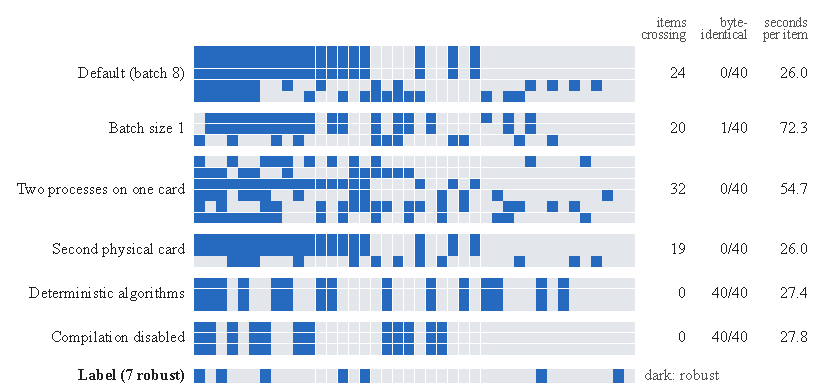
\includegraphics[width=\linewidth]{fig_rumore.pdf}
\caption{Predictions of the official pipeline for 40 preliminary public problems (columns) in 23 executions on DeepSeek (rows), by configuration; the last row is the label, dark cells are robust, and columns are sorted by how often they are predicted robust. At right: items whose prediction changes across the configuration's runs (more runs, more crossings), items whose generated text is byte-identical in all of them, and seconds per item.}
\label{fig:noise}
\end{figure}

\begin{table}[t]
\caption{Repeatability of the official pipeline on DeepSeek, 40 public problems, by configuration, in the order of Figure~\ref{fig:noise}. ``Crossings'': items whose prediction changes across the configuration's runs. ``Identical'': items whose generated text is byte-identical in all runs. Cost is runtime against the default configuration. Card 0 and card 1 are the two GPUs of the same machine. With two processes on one card, any five of its six runs give 29 to 31 crossings.}
\label{tab:reexec}
\centering
\small
\begin{tabular}{@{}lllllll@{}}
\toprule
\textbf{Configuration} & \textbf{Card} & \textbf{Runs} & \textbf{Crossings} & \textbf{Identical} & \textbf{Correct per run} & \textbf{Cost} \\
\midrule
Default (batch 8) & 0 & 5 & 24/40 & 0/40 & 24, 24, 24, 23, 24 & reference \\
Batch size 1 & 0 & 3 & 20/40 & 1/40 & 20, 21, 24 & +178\% \\
Two processes on one card & 0 & 6 & 32/40 & 0/40 & 24 to 28 & +110\% \\
Second physical card & 1 & 3 & 19/40 & 0/40 & 24, 24, 21 & +0\% \\
Deterministic algorithms & 0 & 3 & 0/40 & 40/40 & 24, 24, 24 & +5\% \\
Compilation disabled & 1 & 3 & 0/40 & 40/40 & 25, 25, 25 & +7\% \\
\bottomrule
\end{tabular}
\end{table}

\paragraph{Two candidate remedies.} Deterministic algorithms (PyTorch's, in warn-only mode, with deterministic cuDNN and a fixed cuBLAS workspace; Appendix~\ref{app:C}) and disabled compilation each made the generated text byte-identical in three sequential runs, at 5 to 7\% runtime cost. On card 0, the default configuration produced 24 crossings in five runs. Each remedy ran on one card where the default had produced crossings, each run in a new process, with no other process on that card. Three identical runs are weak evidence: the default configuration also gave three identical runs on card 0 before its fourth diverged, and five of its eight runs on the two cards shared one output. The two remedies produced different outputs, predicting 15 and 12 of the 40 problems robust, and because they ran on different cards we cannot tell whether the difference comes from the configuration or from the card. Neither gained more than one item (24 and 25 correct).

\paragraph{Distinct outputs.} The 23 executions fall into 14 distinct outputs, byte-identical within each. The same output appeared on both cards, and two runs launched in the same second on one card produced different outputs, so the output is not a property of the card alone; what selects it is not established. As only 7 of the 40 problems are robust and crossings largely cancel, accuracy moved much less than predictions: 21 to 24 correct in the default configuration on either card and 24 to 28 with two processes on one card, always below the 33 of the majority constant. An exploratory repetition of the official score extraction, whose third run ranks the 164 labeled problems at Spearman 0.24 against the first two, is in Appendix~\ref{app:C}.

\section{Regenerating the labels with our own protocol}\label{sec:labels}

\paragraph{Our labeling protocol.} We identified the organizers' perturbation families in the preliminary data (rephrase, rename, domain, distract, typos), regenerated them with gpt-oss-120b prompted with public examples, and gated each variant with gpt-oss-120b. An answer counts as correct when it matches gpt-oss-120b's answer on the original problem, because the preliminary data carry no answers; we did not check this key against the answers of the collections the problems come from. On the organizers' machine, with vLLM 0.28.0 [8] outside the official image, we labeled four models with two independent draws of variants (A and B, about 40 accepted variants per problem): 10 samples on the base problem and one per variant, at temperature 0.6, top-p 0.95 and at most 16,384 new tokens. Draw A's variants were also re-sampled with a new seed (A$'$). A label is robust when at least 6 of the 10 base samples are correct and every variant is answered correctly; unlike the earlier rule's conjunction, this requires the base problem to be solved.

A chain that reaches our cap is scored by the last boxed answer it contains, and counts as wrong without one; the organizers also count a response that reaches their limit without a parseable final answer as wrong [4]. Our protocol differs from the organizers' in perturbations, answer key, rule and sampling (one answer per variant, against 10 in the files behind most of their DeepSeek labels). Its decoding differs from the settings they publish, and its prompt may differ from the one behind their labels, which they have not stated.

\begin{table}[t]
\caption{Agreement of labels regenerated with our protocol: Cohen's kappa. The three columns for A and B treat variant chains that reached the 16,384-token cap in three ways: scored as in the protocol (by their last boxed answer, if any), dropped, or all counted as correct. The first of these columns and the A and A$'$ column give 95\% percentile bootstrap intervals over problems, and the script of Appendix~\ref{app:E} gives them for the other two. A problem has a label in a draw when it has at least one accepted variant (160 in A, 159 in B). Kappa between A and B uses the 159 problems labeled in both (150 for Qwen3.5-4B and 156 for DeepSeek when truncated chains are dropped), and between A and A$'$ 160. ``At cap'': percentage of variant chains that reached the cap in draws A and B. ``Robust'': percentage of problems labeled robust in draw A, as scored. The last column gives kappa of draw A with the organizers' preliminary DeepSeek labels: on the 138 published ones, and on the 160 that include 22 labels we derived (Section~\ref{sec:data}).}
\label{tab:label}
\centering
\small
\setlength{\tabcolsep}{3pt}
\begin{tabular}{@{}llllllll@{}}
\toprule
& & & \multicolumn{3}{l}{\textbf{A and B, truncated variant chains}} & & \\
\cmidrule(lr){4-6}
\textbf{Model} & \textbf{At cap} & \textbf{Robust} & \textbf{as scored} & \textbf{dropped} & \textbf{correct} & \textbf{A and A$'$} & \textbf{Organizers'} \\
\midrule
Skywork & 1.2, 1.5 & 74 & 0.44 [0.28, 0.59] & 0.39 & 0.39 & 0.79 [0.67, 0.89] & none \\
DeepSeek & 5.1, 6.1 & 39 & 0.41 [0.26, 0.55] & 0.35 & 0.36 & 0.46 [0.33, 0.59]$^{*}$ & 0.011; 0.025 \\
Olmo & 1.1, 0.9 & 68 & 0.38 [0.21, 0.54] & 0.39 & 0.39 & 0.65 [0.52, 0.78] & none \\
Qwen3.5-4B & 22.1, 29.2 & 9 & 0.18 [$-$0.06, 0.39] & 0.26 & 0.44 & not run & none \\
\bottomrule
\end{tabular}
\par\smallskip{\footnotesize $^{*}$On DeepSeek, A$'$ also received the answer-format line (end of this section), so this entry mixes seed and prompt.}
\end{table}

\paragraph{Results.} Under our protocol, two independent draws of variants give labels that agree at kappa 0.35 to 0.44 on Skywork, Olmo and DeepSeek, whether truncated variant chains are scored as in the protocol, dropped or all counted as correct (Table~\ref{tab:label}). On Qwen3.5-4B, 22 to 29\% of the variant chains reach the cap. Scoring these chains as in the protocol, dropping them or counting them all as correct gives agreement of 0.18, 0.26 and 0.44, and a robust share in draw A of 9\%, 83\% and 79\%. On Skywork, re-sampling the same variants with a new seed agrees far more than drawing new variants (0.79 against 0.44), so its label depends more on the variants than on the seed; on Olmo the gap is smaller (0.65 against 0.38), and on DeepSeek, where A$'$ also changed the prompt, it is 0.46 against 0.41.

Draw A's DeepSeek labels agree with the 138 labels the organizers published at kappa 0.011 [$-$0.13, 0.17], and with the 160 that include 22 of our derived labels at 0.025 [$-$0.12, 0.18]. Of the 36 problems with a published robust label, draw A calls 20 non-robust, and 4 of these change when truncated variants all count as correct. Of the 102 with a published non-robust label, draw A calls 44 robust. The reliability of the organizers' labels remains unmeasured. A retrospective calculation on the same saved answers with the main-phase threshold rule, applied as its pre-registration fixed it, with no filter on the base problem (Appendix~\ref{app:C}), gives test-retest point estimates between 0.34 and 0.56, below the pre-registered bar of 0.60, though three of the four intervals include it.

\paragraph{The prompt changes our labels.} In a first run with the bare problem text, later discarded, \mbox{Qwen3.5-4B} gave a final answer in the expected format in only 5 of its 1,640 base samples in draw A. With one instruction line requesting the format, 145 of 164 problems passed the base condition, against none. DeepSeek passed it on 147 of 164 with or without that line; its draws A and B ran without the line and A$'$ with it, and on the same variants its robust share moved from 39\% to 51\% of the 160 labeled problems, a change that mixes prompt and seed. Under our protocol, the label of Qwen3.5-4B therefore depends on the prompt. Whether this affects the organizers' labels is unknown: their baselines repository has a solve prompt that asks for an ANSWER line, but they have not said whether it was used for labeling (R3).

\section{The falsification campaign}\label{sec:campaign}

Table~\ref{tab:campaign} summarizes the campaign; Appendix~\ref{app:A} lists all 31 entries and explains three traps (rule T, the oracle H13, the duplicated pairs behind H2) and two pitfalls of the data. All entries use the preliminary data, except H16 to H18, which were scored on the 17 items of the warmup evaluation task.

\begin{table}[t]
\caption{The campaign in brief, in 19 of its 31 entries (Appendix~\ref{app:A} lists all). Ground truth is DeepSeek's and the preliminary pairs' unless stated; accuracy differences are in points against each pre-registration's baseline. H1, H7 and T count the 52 duplicated DeepSeek pairs twice; counted once, no verdict changes.}
\label{tab:campaign}
\centering
\small
\begin{tabular}{@{}L{5.5cm}L{1.9cm}L{5.6cm}@{}}
\toprule
\textbf{What we tested} & \textbf{Entries} & \textbf{Outcome} \\
\midrule
Text features; robustness as a property of the problem; labels, base accuracy and difficulty order across models & H1 to H5, H7 & rejected; H2 gained only when the duplicated pairs were counted twice \\
Official uncertainty features, logistic regression & H10 & 0.774 against a majority constant of 0.756, within the 0.692 $\pm$ 0.101 of the proposal [1] (method substituted) \\
Features cached for other models; per-target thresholds & H12, H13 & H12 rejected; the H13 ceiling withdrawn, $-$2.8 points when forced to rank \\
Our perturbation families, translation, self-consistency, the organizers' families regenerated (pilot), representation shift & H19, H22, H30 to H33 & rejected: kappa at most 0.02, AUROC at most 0.615 \\
Probes on DeepSeek's hidden states: ours and the organizers' published artifact & H36, H35 & survive their nulls; ours adds no detectable gain over length, and the artifact's score is probably in-sample \\
Trivial-robust rule, post hoc & T & a trap: +6.0 points on the preliminary pairs, +0.0 on \texttt{val-sample} \\
Identical bundles re-executed (warmup, 17 items) & H18 & noise confirmed: 11, 9, 11 and 11 correct \\
\bottomrule
\end{tabular}
\end{table}

\paragraph{Length and probes.} The character count of the problem alone orders the 164 DeepSeek labels at AUROC 0.704. Our logistic probe on DeepSeek's last-token hidden states, with layer and regularization chosen by inner cross-validation, reaches 0.710 out of fold with the original fold assignment. Over 20 other assignments, passed through the second-stage model below, it gives 0.57 to 0.76 (mean 0.69). Its scores correlate with length at Spearman +0.55, and residualized on log character count it gives 0.62. Its permutation null, rerun with 1{,}000 permutations of the whole nested procedure (the first version used 60, where 500 were pre-registered), gives $p = 0.002$. Restricted to the 138 published labels, these out-of-fold scores give 0.714 and length 0.733; retrained on those 138 alone with H36's procedure and seed, the probe gives 0.620. Combined with length in a second-stage model fitted on common outer folds, the probe changes AUROC over length alone by +0.005 on the 164 labels and by $-$0.010 on the 138 published ones (median bounds of the per-assignment 95\% intervals: $-$0.03 to 0.04, and $-$0.04 to 0.02): we detect no gain from adding the probe to length (Appendix~\ref{app:C}). This analysis replaces an earlier combination that leaked labels (Appendix~\ref{app:D}).

The organizers' published DeepSeek probe artifact orders the 164 DeepSeek labels at 0.739 with the aggregation we pre-registered and at 0.709 with its own, and at 0.62 and 0.57 residualized on log character count; its controls trained on shuffled labels give 0.68 at layer 31. The artifact does not record its training data; we infer that 137 of the 164 problems were among the public rows it was trained on, so these scores are probably largely in-sample. These length controls, which play the role of control tasks [7], were post hoc. Whether either probe reads anything beyond length that bears on robustness is not established. Apart from the three traps of Appendix~\ref{app:A}, no signal we scored by accuracy beats the majority constant by more than about one standard error on the preliminary labels, most of them DeepSeek's.

\section{Our entries}\label{sec:entries}

Our entry V8, pre-registered on 13 September, is the whole rule \texttt{return~[len(p)~>=~98 for~p~in~problems]}, with the threshold at the lower median of the 174 preliminary problems and the direction fixed on the preliminary pairs. On the original main-phase tasks it scored 11/21 and 10/19, like our entry v6 and the organizers' own entries. None of these beat the majority constant, which scores at least 11/21 and 10/19 on these tasks, and on so few items the ties do not show that length carries no signal (95\% Wilson intervals 0.32 to 0.72 and 0.32 to 0.73). On the 71 labeled rows of the official training set (revision of 17 September; 36 distinct problems), V8 differs from the all-robust constant on only 6 rows and is wrong on all 6 (46/71 against 52/71): too few to say what length is worth on official data. On the replacement tasks of 16 September, before and after the evaluation changed on 15 October [6], it predicted robust for every item (10/21 and 7/14), like an all-robust control. For the final test we nominated V8 (Codabench 1016713) and the constant (1016732), both on the Main track; our pre-registered predictions will be scored there (Appendix~\ref{app:B}).

\section{Recommendations}\label{sec:recs}

These rest mostly on DeepSeek and the preliminary data, and should be checked on the other models.
\begin{itemize}
\item \textbf{R1. Remove the variation between runs, and test the remedy:} on the same card with independent restarts, under load and across cards.
\item \textbf{R2. Repeat only where it decides something:} at the warmup's re-execution noise (a standard deviation of 1.0 item on 17, itself estimated from four runs), a one-item gap needs about eight runs per entry to reach two standard errors, so repeat only entries that run a model and sit near a prize boundary.
\item \textbf{R3. Say which prompt and decoding settings produced each released label file,} at least after the close.
\item \textbf{R4. Measure the label's reliability directly,} with two independent draws of variants labeled by the official process.
\item \textbf{R5. Show floors and noise on the leaderboard:} a row per constant predictor, the re-execution noise and binomial intervals.
\item \textbf{R6. Require a length control in white-box ablations.}
\item \textbf{R7. Remove the leaking field} \texttt{permutation\_type} from the aggregated datasets (Appendix~\ref{app:A}).
\end{itemize}

\paragraph{Code and data.} Our code, bundles, pre-registrations and outcome files are released at \href{https://github.com/Dan23RR/aimo-instrument}{\nolinkurl{github.com/Dan23RR/aimo-instrument}}. Its folder \texttt{reproduce/} recomputes the main tables from saved outputs and the six preliminary datasets, and the other numbers come from the dated records in \texttt{archive/} (Appendix~\ref{app:E}).

%%%%%% End of the main text: the six pages end here; the Limitations do not count %%%%%%
\label{fine-testo}

\section*{Limitations}

\begin{enumerate}[leftmargin=1.6em, itemsep=2pt, topsep=4pt, parsep=0pt]
\item \textbf{Preliminary data, not official data.} We did not repeat our label and probe analyses on the official training set, beyond the evaluation of V8 and a five-row check of our labels (Appendix~\ref{app:C}). Findings on label reliability and predictability may not generalize to the official evaluation setting.
\item \textbf{Our protocol, not the official one.} We did not regenerate labels with the organizers' published settings (100,000 tokens, temperature 1.0), with 10 answers per variant as in the files behind most DeepSeek labels, or on \texttt{train-main-v2}. The three treatments of truncated variant chains show how much our cap moves agreement between our draws; all three score base samples that reach the cap as the protocol does, and none of them reproduces longer decoding or a different temperature. Our low agreement with the organizers' labels is a fact about our process.
\item \textbf{One model.} We ran the probes, the re-execution study of Section~\ref{sec:reexec} and the comparisons of our regenerated labels with the organizers' preliminary labels only on DeepSeek.
\item \textbf{Re-execution.} We did not run the two candidate remedies on the same card, so card and configuration are confounded; we did not test either remedy under contention or on both cards, and we used 40 problems and one image.
\item \textbf{Records.} Some analyses rest on re-created scripts or dated records (Appendix~\ref{app:D}). Nothing here estimates performance on the final held-out problems.
\end{enumerate}

\section*{AI usage statement}

In this work, we used one generative AI tool, Claude (Anthropic), through Claude Code, for ideation, coding, analysis and writing. Ideation: it drafted the pre-registrations, including hypotheses, predictions and kill criteria, and searched and summarized the literature and the public records, including the organizers' Discord channels and the author's correspondence with them. Coding: it wrote the solution code of our bundles and the analysis and extraction scripts, ran them, and operated the organizers' virtual machine over SSH. Analysis: it computed and interpreted the results and ran automated adversarial reviews of hypotheses, drafts and code. Writing: it drafted the correspondence, this report and its revision after review.

It also made most of our Codabench uploads through the author's browser at the author's instruction. There were two exceptions: one resubmission (925822, 14 September), made without a specific instruction, and one submission that the author had not approved, sent in error and rejected before import (1016734, 28 October).

Language models were also components of our method: gpt-oss-120b generated and gated the perturbation variants and supplied the reference answers of Section~\ref{sec:labels}, and phi-4 translated problems for H22. The final decisions on the direction of the work, on the submissions (with the two exceptions above), on the nominations for the final test and on the claims of this report were the author's, and the author sent all correspondence personally. The author has reviewed all AI-assisted work and takes full responsibility for the final content of this report.

\begin{ack}
We thank Michal Štefánik, Róbert Belanec and the AIMO Interpretability team for the compute grant, a virtual machine with two GPUs, and for answering our questions; on 2 November they confirmed that the measurements taken on their machine may appear in this report. We also thank the three reviewers and the program chairs: two reviewers checked our analyses against the released code and data, and their checks corrected several of our claims. Other GPU time was rented on Modal and paid by the author or covered by Modal's platform credit. This work received no other funding, and the author has no competing interests.
\end{ack}

\section*{References}
{\small
[1] M. Štefánik, P. Mondorf, A. Waldis, Q. Liu, C. Yang, M. Spiegel, J. Kuchař, M. Kadlčík, A. Vawda-Oomerjee, C. Liu, S. Frieder, B. Plank, F. Barez and P. Stenetorp. AIMO Interpretability Challenge. CoRR, abs/2607.13899, 2026. doi:10.48550/arXiv.2607.13899.

[2] H. He and Thinking Machines Lab. Defeating Nondeterminism in LLM Inference. Thinking Machines Lab: Connectionism, 2025.

[3] J. Yuan, H. Li, X. Ding, W. Xie, Y.-J. Li, W. Zhao, K. Wan, J. Shi, X. Hu and Z. Liu. Understanding and Mitigating Numerical Sources of Nondeterminism in LLM Inference. NeurIPS 2025. arXiv:2506.09501.

[4] AIMO Interpretability Challenge website and FAQ. \url{https://aimo-interp.github.io} (accessed 28 October 2026), and its source repository aimo-interp/aimo-interp.github.io on GitHub.

[5] aimo-interp/getting-started and aimo-interp/baselines, GitHub repositories: README and issues \#6 and \#10 of getting-started; aimo-interp datasets on Hugging Face, including \texttt{train-main-v2} and \texttt{val-sample}.

[6] AIMO Interpretability Challenge Discord, \#announcements and \#qa: 5, 15 and 22 September, 9, 15, 16 and 20 October 2026.

[7] J. Hewitt and P. Liang. Designing and Interpreting Probes with Control Tasks. EMNLP-IJCNLP 2019.

[8] W. Kwon et al. Efficient Memory Management for Large Language Model Serving with PagedAttention. SOSP 2023.

[9] D. Hendrycks et al. Measuring Mathematical Problem Solving With the MATH Dataset. NeurIPS 2021 Datasets and Benchmarks Track. arXiv:2103.03874.
}

%%%%%% End of the references %%%%%%
\clearpage
\appendix
\raggedright

\section{The hypotheses, three traps and two pitfalls of the preliminary data}\label{app:A}

Section~\ref{sec:campaign} summarizes these entries. Unless stated, the ground truth is the 335 public pairs for H1 to H9 and T, the other models' preliminary labels for H12 to H15, the 17 items of the warmup evaluation set for H16 to H18, and DeepSeek's labels for the others. Validation that fits on some problems and tests on others is grouped by problem. The cross-model tests H7 and H12 to H15 hold out the model but not the problem, so part of them is in-sample; H7, H12, H14 and H15 were rejected anyway, and H13 is withdrawn. Numbers are accuracy points against each pre-registration's baseline unless they are kappa or AUROC.

{\small\setlength{\tabcolsep}{4pt}\renewcommand{\arraystretch}{1.2}
\begin{longtable}{L{1.1cm}L{3.9cm}L{5.6cm}L{2.0cm}}
\toprule
\textbf{ID} & \textbf{Hypothesis} & \textbf{Result} & \textbf{Verdict} \\
\midrule
\endfirsthead
\toprule
\textbf{ID} & \textbf{Hypothesis} & \textbf{Result} & \textbf{Verdict} \\
\midrule
\endhead
\bottomrule
\endlastfoot
H1 & The problem text predicts robustness (32 features) & 0.675 against 0.761, $-$8.7 ($-$7.4 with the duplicated pairs counted once) & rejected \\
H2 & Robustness is a property of the problem & with the 52 duplicated pairs counted once, z~=~0.88 and $-$1.3 against the per-model majority (bar 4.0); z~=~4.04 and +3.4 only when they are counted twice & rejected \\
H3 & One model's label predicts another's & $-$7.3 & rejected \\
H4 & One model's base accuracy predicts another's robustness & $-$11.8 & rejected \\
H5 & The difficulty order transfers across models & $-$25.4 & rejected \\
H6 & The same, with the oracle number of positives & $-$13.0 & ceiling (no kill criterion) \\
H7 & Base accuracy beats the prior on held-out models & $-$1.2 against the per-model majority that its pre-registration named (+0.0 against the global prior we used instead) & rejected \\
T & Robust if and only if base accuracy is below 0.05 (post hoc; see the traps below) & +6.0 on the 335 public pairs, +0.0 on \texttt{val-sample} & trap (no kill criterion) \\
H10 & The official uncertainty features reach the accuracy the proposal reports & 0.774 against a majority constant of 0.756, within 0.692 $\pm$ 0.101 [1]; a logistic regression on 13 of the 14 features of our own A100 re-implementation of the extraction (three of them constant), substituted for the official regressor & confirmed (method substituted, not declared at the time) \\
H11b & Length, saturation and trend features add signal & $-$1.8 and $-$2.5 & rejected \\
H12 & A cached model's uncertainty features predict other models & $-$16.5 & rejected \\
H13 & The same, with a threshold chosen per target & +7.3, from thresholds chosen on the scored items; $-$2.8 when forced to rank & withdrawn (no kill criterion) \\
H14, H15 & Calibration by the target's rate or by the global rate & $-$2.8 and $-$10.1 & rejected \\
H16 & Every model measured by itself beats the constant & 10/17 against 9/17 on one execution, inside the noise of H18 & survives, within noise \\
H17 & A gpt-oss threshold calibrated on \texttt{val-sample} beats H16 & 11/17, then 9, 11 and 11 on re-execution; 9/17 meets the kill criterion & not established \\
H18 & Identical bundles score differently across executions & 11, 9, 11 and 11 correct & confirmed (no kill criterion) \\
H19 & Our five mechanical perturbation families reproduce the organizers' preliminary label & accuracy 0.354 against 0.788, kappa 0.02 & rejected \\
H20 & A threshold tuned on our label transfers & 0.212 against 0.788 & rejected \\
H22 & Stability under translation reproduces the organizers' preliminary label & 0.507 against 0.740, kappa $-$0.10 & rejected \\
H23 & A threshold tuned on it transfers & +0.0 & rejected \\
H29 & Representation-distance features are repeatable (gate; written plan, not a frozen pre-registration) & ICC 0.997 to 0.999, from the dated outcome file & passes \\
H30 & The representation shift under perturbation predicts the label (written plan) & AUROC 0.615, below the kill threshold of 0.655; character count 0.704 (0.705 in E11's own computation) & rejected \\
H31 & The direction of that shift predicts the label (written plan) & AUROC 0.555 & rejected \\
H32 & The organizers' families, regenerated (pilot), reproduce their label & kappa $-$0.001 on four families, $-$0.030 with all five & rejected \\
H33 & Self-consistency over 8 samples predicts the label & AUROC 0.502 & rejected \\
H35 & The organizers' published probe artifact orders the 164 DeepSeek labels & 0.739 under the pre-registered aggregation and 0.709 under its own; 0.62 and 0.57 once residualized on log character count; its shuffled-label controls give 0.68 at layer 31 & survives its null; probably in-sample, not separated from length \\
H36 & Our linear probe, nested cross-validation, orders the 164 DeepSeek labels & 0.710 out of fold, above its permutation null, and 0.62 once residualized on log character count; 0.714 against 0.733 for length on the 138 published labels (Appendix~\ref{app:C}) & survives its null; no detectable gain over length \\
E13b-1 & Under the main-phase rule our regenerated label is test-retest reliable (kappa at least 0.60 on 3 of 4 models) & 0.34 to 0.56, retrospective (Appendix~\ref{app:C}) & rejected \\
E13b-2 & Under the main-phase rule it agrees with DeepSeek labels we computed with that rule from the preliminary data (kappa at least 0.40) & 0.02 [$-$0.09, 0.13] & rejected \\
E13b-3 & The labeling rule drives the instability of our regenerated labels & a gain of at least 0.15 on 2 of 4 models, where 3 were required; 0 of 4 on common problems & rejected \\
\end{longtable}
}

Not in the table are H8, H9, H21, H24 and H25 to H28. H8 is an oracle ceiling: 0.774, +1.8 points against the global constant and +0.4 against the per-model majority, with the duplicated pairs counted once. The outcome of H9 became rule T. H21 and H24 needed H19 and H20, and H22 and H23, to survive, so they were not run. H25 to H28 are entries of the E11 plan that its outcome file does not report under these identifiers. H25 is an anomaly of our own re-implementation of the extraction, found before the plan. H26 is the list field of the first pitfall below. H27 is a label-noise ceiling, which the plan itself closed with a resampling estimate instead of a test. H28 is the text-only baseline, which became character count (Appendix~\ref{app:D}). Three further E11 tests were not run (Appendix~\ref{app:D}). V4, an entry submitted once against its own pre-registered rule, is in Appendix~\ref{app:D}.

\paragraph{Three traps.} Rule T gains six points on the public pairs and nothing on \texttt{val-sample}, because the trivially robust items (base accuracy 0, robust under the conjunction) are absent there. The oracle H13 chose each target's threshold among all cut points on the very items it was scored on; forced to rank the items and to predict the true number of positives, it gave $-$2.8. H2 owed its survival to one measurement published under two model names and counted twice; counted once, its z falls from 4.04 to 0.88.

\paragraph{Two pitfalls of the preliminary data.} In the three aggregated datasets, the field \texttt{permutation\_type} is a list if and only if the item is robust, because the aggregation merges all perturbation types into one row for robust items and keeps one row per retained type otherwise, usually a single type. The rule ``robust if the field is a list'' reproduces all 223 labeled rows of the three datasets, and the field does not exist at inference (recommendation R7). And 20 of the 80 robust pairs among the 335 have base accuracy 0. None of them carries a published label, so they are robust only under the conjunction we used to derive their labels, while \texttt{val-sample} has no labeled pair with base accuracy below 0.05.

\section{Pre-registered predictions for the final evaluation}\label{app:B}

P1 was written on 7 September 2026, P-V8 on 13 September and P-V8b on 21 September. They are translated from the dated files and shortened. We omit the runtime predictions (under 60 seconds), which we could not score because the bundles log no runtime. A second prediction written with P1 on 7 September concerns another participant's final score and is not reported here.

\begin{itemize}
\item \textbf{P1.} The top-ranked entry's accuracy on the final held-out problems will lie within two binomial standard errors of that set's majority-class constant.
\item \textbf{P-V8.} If the organizers had neutralized length, V8 would score between 0.45 and 0.55 on both tracks (stated beforehand as the most likely outcome); if they had not, and the set was balanced, about 0.66. Observed on the original tasks: 0.52 and 0.53, inside the first band; on 21 and 19 items, however, 0.66 lies inside the 95\% intervals of both scores, so the scores do not exclude the second.
\item \textbf{P-V8b}, on the replacement tasks: the same bundles work with the new ingestion and score 6 to 15 of 21 and 4 to 10 of 14. Observed: coverage 1.0, no invalid predictions, 10/21 and 7/14, inside the bands but degenerately, since the rule predicted robust for every item.
\end{itemize}

\section{Protocols, run manifest and recalculations}\label{app:C}

\paragraph{Hardware and software.} The generation runs used the organizers' virtual machine with two NVIDIA RTX PRO 6000 Blackwell Server Edition GPUs (96 GB each), the evaluation workers' model, from 8 September 2026. Each run used one GPU; the Olmo-3-7B-Think A$'$ labels combine two runs, one on each card (below).
\begin{itemize}
\item \textbf{Official runtime image.} Section~\ref{sec:reexec} and the official score channel (E16) ran inside it: {\footnotesize\path{ghcr.io/aimo-interp/aimo-codabench-runtime:torch2.12.1-cuda13.2-cudnn9-transformers5.13.0-sklearn1.8.0-kernels0.15.2}}, digest {\footnotesize\path{sha256:fb4dab6343de7ce022ddd7906493f9ced16ff9008d497326a781d1e5adc8207a}}. They used the official extraction and regressor as shipped in our bundles: greedy decoding, at most 4,096 new tokens, static cache, batch 8.
\item \textbf{Labeling environment.} Section~\ref{sec:labels} ran with vLLM 0.28.0, torch 2.13.0 and transformers 5.16.1 (driver 610.57.04 with CUDA 13.3 on the machine, CUDA 13.0 runtime libraries in the environment) in a separate environment on the same machine; \texttt{vm\_backup/AMBIENTE\_VM\_2026-09-17.txt} lists every package.
\item \textbf{Model revisions.} Hugging Face snapshot hashes: Qwen3.5-4B \texttt{851bf6e8}, Skywork-OR1-Math-7B \texttt{fcef970f}, Olmo-3-7B-Think \texttt{d97e442d}, DeepSeek-R1-0528-Qwen3-8B \texttt{6e8885a6}, gpt-oss-120b \texttt{b5c939de}. The full hashes are in the run logs.
\item \textbf{Analyses.} They ran on CPU: E13's analysis and E15's evaluation, up to 14 September, on the virtual machine (Python 3.12, NumPy 2.3.5, scikit-learn 1.9.1), the others on the author's computer (Python 3.11.12, NumPy 2.4.4 and scikit-learn 1.8.0, as recorded for the runs of September and November). The release pins every output by SHA-256 in \texttt{MANIFEST.tsv}.
\end{itemize}

\needspace{8\baselineskip}
\paragraph{Run manifest.}
\begin{itemize}
\item \textbf{Where they ran.} The scripts in \texttt{vm/} written up to 14 September (setup, generation, extraction, E13's analysis and E15's evaluation), after which the machine stayed idle, and the clean-up script of 17 September ran on the virtual machine; the later ones ran on the author's computer.
\item \textbf{Outputs} are in \texttt{vm\_risultati/} unless the table gives another path.
\item \textbf{GPU-hours} are times from the logs (\texttt{reproduce/compute\_hours.py}). They include model loading except for the E13 labels, a difference under 1\%.
\end{itemize}

{\small\setlength{\tabcolsep}{4pt}
\begin{longtable}{L{2.4cm}L{3.2cm}L{2.2cm}>{\raggedright\arraybackslash\footnotesize}p{4.8cm}}
\toprule
\textbf{Run} & \textbf{Where it ran} & \textbf{GPU-hours} & \textbf{Outputs} \\
\midrule
\endfirsthead
\toprule
\textbf{Run} & \textbf{Where it ran} & \textbf{GPU-hours} & \textbf{Outputs} \\
\midrule
\endhead
\bottomrule
\endlastfoot
E13 variants & virtual machine & 1.15 and 1.20 & \path{e13/varianti_D1.parquet}, \path{e13/varianti_D2.parquet} \\
E13 labels & virtual machine, one queue per card & 64.4, in the logs of the 11 runs of Table~\ref{tab:label} & \path{e13/etich_*.parquet} \\
E13b, main-phase rule & author's computer & CPU only & \path{e13b_regola_nuova_2026-09-21.txt} \\
E14 re-execution & virtual machine, official image & 8.4 & \path{e14/out/*.jsonl}, \path{e14/log/} \\
E15 extraction & virtual machine & under 0.1 & \path{vm_backup/estratto/work/aimo/e15/hs_*.npz} \\
E15 probes & the virtual machine's CPU on 14 September, then the author's computer & CPU only & \path{e15_*}, \path{e15r/}, \path{vm_backup/estratto/work/aimo/e15_valuta.log} \\
E16 score channel & virtual machine, official image & 5.9 & \path{e16_*.jsonl}, \path{e16nodet/} \\
\end{longtable}
}

\paragraph{Commands.} Script paths are relative to \texttt{archive/}, the working folder of the repository. The scripts in \texttt{vm/} that ran on the virtual machine use paths under \texttt{/work/aimo}. \texttt{M} stands for the model, and in E14 \texttt{C}, \texttt{r}, \texttt{g} and \texttt{t} for the configuration, repetition, card and process tag.
\begin{itemize}
\item \textbf{E13 variants.} \texttt{vm/e13\_varianti.py -{}-draw~D1 -{}-seed~20260913 -{}-n~164 -{}-k~10}, and \texttt{-{}-draw~D2 -{}-seed~20260914}. The model gpt-oss-120b generates, solves and gates the variants (prompts below).
\item \textbf{E13 labels.} DeepSeek A and B ran an earlier version of \texttt{e13\_etichetta.py} that sent the bare problem text (now \texttt{-{}-prompt~nudo}); every other run behind Table~\ref{tab:label}, DeepSeek A$'$ included, used the explicit prompt. Draw A: \texttt{vm/e13\_etichetta.py -{}-model~M -{}-cond~A -{}-draw~D1 -{}-seed~20260921 -{}-prompt~esplicito}; B: \texttt{-{}-cond~B -{}-draw~D2 -{}-seed~20260922}; A$'$: \texttt{-{}-cond~Ap -{}-draw~D1 -{}-seed~20260923}. \texttt{vm/e13\_coda.sh} launched one queue per card (its logs are in \path{vm_backup/estratto/work/aimo/}); the card 0 queue ran an earlier version that passed no \texttt{-{}-prompt} flag, so DeepSeek A$'$ got the default of \texttt{e13\_etichetta.py}, the explicit prompt.
\item \textbf{E13b.} \texttt{vm/e13b\_regola\_nuova.py}, on the saved E13 answers; retrospective (below).
\item \textbf{E14.} \texttt{vm/e14\_all.sh 40 "C0 C1 C2 C3"} and \texttt{vm/e14\_extra.sh 1 "C5 C4"}. Each run is \texttt{e14\_run.py -{}-cond~C -{}-rep~r -{}-gpu~g -{}-tag~t -{}-n~40} inside the official image: 23 runs on DeepSeek. In the 8.4 GPU-hours the two processes of each contention pair, which shared one GPU, count once (20 runs).
\item \textbf{E15 extraction.} \texttt{vm/e15\_estrai.py -{}-model~deepseek-ai/DeepSeek-R1-0528-Qwen3-8B}, with and without the official system prompt: one forward pass per problem, last input token, all 37 hidden-state indices, at most 2,048 tokens.
\item \textbf{E15 probes.} \texttt{vm/e15\_valuta.py} ran H35, H36 and the first null (60 permutations) on 14 September, on the virtual machine's CPU; its log is \path{vm_backup/estratto/work/aimo/e15_valuta.log}. The file \path{vm_risultati/e15_valuta_2026-09-14.txt} is a later run of that day, by the file times in \path{vm_backup/MANIFEST_backup_aimo_2026-09-17.txt}, that stopped with an error at the null. H35's null is the 95th percentile, 0.602, of the AUROC of 20{,}000 random scores on the same labels, in either orientation. \texttt{vm/e15\_null\_nidificato.py} reran that null on 23 September with both grids of $C$, on the author's computer. E15-R (below) is \texttt{vm/e15r\_ricalcolo.py}, given an output folder and a number of worker processes (5 on the author's computer, 14.5 hours); its outputs are in \texttt{vm\_risultati/e15r}, and since it appends to existing files, a rerun needs a new folder. H35 needs the organizers' artifact \texttt{probe\_artifact.pkl} (hash below), which we do not redistribute.
\item \textbf{E16.} \texttt{vm/e16\_all.sh} and \texttt{vm/e16\_nodet.sh}, in the official image. Of the variables that \texttt{e16\_all.sh} sets, only the cuBLAS workspace variable reaches the extraction; \texttt{e16\_nodet.sh} sets neither.
\end{itemize}

The organizers' artifact used by H35 has SHA-256 {\footnotesize\texttt{8607478c7408922a6490adb7bda34d6a7d95403b7aa62f80dd3f2649139ccdeb}}. The listed logs total 82.8 GPU-hours. Not in the table:
\begin{itemize}
\item two complete runs of Qwen3.5-4B with the bare prompt (about 13 GPU-hours, no released log);
\item a partial run of Qwen3.5-4B A$'$ with the bare prompt (1.7 GPU-hours, included in the 82.8), discarded with them;
\item a run of Olmo-3-7B-Think A$'$ on card 1 (11.0 GPU-hours, 07:19 to 18:21 UTC on 10 September, from its queue log). Card 0 reached the same condition at 14:20, resumed from its partial file with 96 of the 164 problems done and finished the other 68, so the reported A$'$ labels come from both cards.
\end{itemize}
With these, the virtual machine ran about 107 GPU-hours, plus short smoke and feasibility tests. Our earlier runs on Modal used about 12 to 13 GPU-hours, mostly on A100 GPUs, as documented in their dated outcome files: the feature extraction behind H10, its pilot, and E9 to E12.

\paragraph{What can be recomputed.}
\begin{itemize}
\item \textbf{From saved outputs.} The scripts in \texttt{reproduce/} (Appendix~\ref{app:E}), which also read the six preliminary datasets; the other numbers come from the dated records in \texttt{archive/}.
\item \textbf{On a CPU, from the released hidden states.} Our probe (H36) and E15-R can be rerun end to end. H35 also needs the organizers' artifact.
\item \textbf{Only with the original GPUs and models.} The generation runs.
\end{itemize}

\paragraph{Re-execution configurations (Section~\ref{sec:reexec}).}
\begin{itemize}
\item \textbf{C0, default:} batch 8, on card 0, five runs.
\item \textbf{C1, batch size 1.}
\item \textbf{C2, deterministic algorithms:} \texttt{torch.use\_deterministic\_algorithms(True, warn\_only=True)}, \texttt{cudnn.deterministic = True}, \texttt{cudnn.benchmark = False} and \texttt{CUBLAS\_WORKSPACE\_CONFIG=:4096:8}.
\item \textbf{C3, contention:} two identical processes at the same time on card 0, three pairs.
\item \textbf{C4, second card:} the default on card 1.
\item \textbf{C5, compilation disabled:} \texttt{TORCH\_COMPILE\_DISABLE=1}, on card 1.
\end{itemize}
Runs within a configuration were sequential, each a new process. During these runs the other card was running another of our jobs. Two pre-registered predictions failed:
\begin{itemize}
\item batch size 1 did not make generation more repeatable: three runs gave three different outputs;
\item disabled compilation was predicted to land in one of the default outputs; it was byte-identical across its runs, but in an output of its own.
\end{itemize}
\texttt{reproduce/reexecution\_table.py} recomputes Table~\ref{tab:reexec} and the numbers of Figure~\ref{fig:noise}, and lists the 14 distinct outputs.

\paragraph{Variants and labels (Section~\ref{sec:labels}).}
\begin{itemize}
\item \textbf{Few-shot pool.} The generator saw five public examples of each family, drawn from a pool of 621 public examples (original, perturbed) over the five families. The texts are the organizers' and are not redistributed. \texttt{vm\_risultati/e13/fewshot\_pool\_ids.json} lists each example's problem identifier and SHA-256 hashes, and \texttt{reproduce/fewshot\_pool.py} rebuilds the pool from the downloaded preliminary datasets (verified on 23 November 2026: 621 of 621, byte-identical).
\item \textbf{Drawing the examples.} For draw seed $s$, problem $p$ and family $f$, the five examples are \texttt{random.Random("s|p|f").sample(pool[f] without p, 5)}.
\item \textbf{Generator.} gpt-oss-120b at low reasoning effort, temperature 1.0, top-p 1.0, at most 4,096 tokens, one request per problem and family, asking for 10 variants.
\item \textbf{Gate and reference answers.} gpt-oss-120b at medium effort, temperature 1.0, at most 8,192 tokens, solves the original and each variant. A variant is accepted if its text differs from the original, the length ratio lies between 0.7 and 4.0, and the solver's answer is unchanged. The solver's answer on the original is the reference answer.
\item \textbf{Labeling.}
  \begin{itemize}
  \item \textbf{Prompt.} Each model receives the instruction line (the second block below) followed by the problem, except DeepSeek in A and B, which received the bare text.
  \item \textbf{Sampling.} Temperature 0.6, top-p 0.95, at most 16,384 new tokens (raised from 8,192 before execution, after a test in which 2 of 3 problems saturated 8,192). There are 10 samples on the base problem and one per accepted variant.
  \item \textbf{Scoring.} A chain is scored by the last boxed answer it contains. Without one, including when it was cut at the cap, it counts as wrong.
  \end{itemize}
\end{itemize}

{\footnotesize
Generator prompt:
\begin{quote}\ttfamily
You create variants of mathematics competition problems for a robustness benchmark. Perturbation type: <family>. <family instruction> The variant must be a complete, self-contained problem with exactly the same final answer as the original. Do not solve the problem. Do not add hints or solutions. Here are 5 examples of this perturbation type: Example 1 Original: <public original> Variant: <public variant> (four more examples) Now write 10 different variants of the following problem. Make them genuinely different from each other. Output each variant between <variant> and </variant> tags, and nothing else. Original: <problem>
\end{quote}
Instruction line of the labeling prompt, also used by the solver of the gate:
\begin{quote}\ttfamily
Solve the following problem. Reason step by step, then give only the final answer inside \textbackslash{}boxed\{\}.
\end{quote}
}
The five family instructions, verbatim:
\begin{itemize}
\item rephrase: ``Rewrite the problem in different words while preserving exactly its mathematical content and its final answer.''
\item rename: ``Rename the variables, people, objects or entities in the problem while preserving its mathematical structure and its final answer.''
\item domain: ``Transfer the problem to a different real-world surface domain (a different story, setting and objects) while preserving exactly the same mathematical structure and the same final answer.''
\item distract: ``Insert irrelevant but plausible additional information (extra facts, numbers or context) that does not change the problem or its final answer.''
\item typos: ``Introduce harmless typographical or formatting noise (misspellings, spacing, punctuation, capitalisation) without changing the meaning of the problem or its final answer.''
\end{itemize}

\paragraph{The main-phase rule, retrospectively (E13b).} PREREG\_E13b was written on 21 September, before any calculation under the main-phase rule but after the E13 answers had been measured, so the calculation is retrospective.
\begin{itemize}
\item \textbf{The rule.} On the saved answers, a problem is robust if the largest drop in accuracy across families is at most 0.10 and non-robust if it is at least 0.25; problems in between get no label.
\item \textbf{No base filter.} As pre-registered, the primary calculation has no filter on the base problem, so a problem the model never solves counts as robust when no family lowers its accuracy.
\item \textbf{Test-retest, primary.} Kappa between A and B is 0.34 [0.13, 0.53] on 86 problems (Qwen3.5-4B), 0.49 [0.17, 0.76] on 132 (Skywork), 0.41 [0.09, 0.69] on 133 (Olmo) and 0.56 [0.36, 0.73] on 100 (DeepSeek). Because 58 to 95\% of the problems are labeled robust, kappa stays low even where raw agreement is high.
\item \textbf{Test-retest, secondary (S1).} On problems with at least 5 of 10 correct base samples in both draws, kappa is 0.31, 0.52, 0.40 and 0.55.
\item \textbf{Against the organizers.} Against DeepSeek labels that we computed with the same rule from the accuracy drops published in the preliminary data: 0.02 [$-$0.09, 0.13] on 133 problems.
\item \textbf{Against \texttt{train-main-v2}.} On its five labeled rows that fall on our problems and models, our labels agree with the official ones on 2 (draw A, one undefined) and 3 (draw B); five rows are too few to read.
\item \textbf{Truncated chains} are scored as in the protocol here too.
\end{itemize}

\paragraph{Subsampling (E13).} Subsampling DeepSeek's variants from 2 to 40 per problem leaves the mean kappa between A and B between 0.36 and 0.47, with no upward trend: more variants per problem do not make our labels more repeatable.

\paragraph{The official score channel (E16, exploratory).} We extracted the official regressor score on DeepSeek three times for the 174 public problems with the same code and image; this measurement was not pre-registered. The first run set the cuBLAS workspace variable and gave the same scores as the second, run without it, on all 174 problems. The second and third correlate at Spearman 0.24 over the 164 labeled problems. They give AUROC 0.487 and 0.602 in the regressor's own orientation; the paired bootstrap 95\% interval of their difference, $-$0.015 to 0.246, includes zero. The ranking of the problems was not reproduced in one of two repetitions; this does not show that the signal itself changes. As 137 of the 164 problems are in the regressor's training set, this concerns the stability of its inputs, not new problems. The 5.9 GPU-hours of the manifest also include one extraction each on Qwen3.5-4B, Skywork and Olmo, which this report does not use, and a failed start on gpt-oss-120b.

\paragraph{E15-R: the probe recalculated after review.} The procedure was fixed in \texttt{vm/e15r\_ricalcolo.py} before it ran, in a run started on 23 November 2026. It uses the same hidden states, labels and nested cross-validation as H36: layers 1 to 36, $C$ in \{0.001, 0.01, 0.1, 1\}, 5 outer and 4 inner folds.
\begin{itemize}
\item \textbf{Combination with length.}
  \begin{itemize}
  \item There are 20 fold assignments on the 164 labels and 10 on the 138 published ones.
  \item The probe's scores for the outer training problems come from a nested cross-validation inside them. Its score for each outer test problem comes from a probe selected and fitted on the outer training problems.
  \item A second-stage logistic regression on log character count, on the probe score, or on both, is fitted on the outer training problems and scored on the outer test problems.
  \item The 95\% interval of the gain of ``both'' over length is a paired bootstrap over problems (2,000 resamples) for each assignment; we report the median of its bounds.
  \end{itemize}
\item \textbf{Retraining.} The nested probe is retrained on the 138 published labels alone.
\item \textbf{Permutation null.} The null of H36 is extended from 60 to 1,000 permutations of the whole nested procedure, with the seeds of the first 60 unchanged.
\end{itemize}
We fixed the decision rule before the run: if the interval of the gain includes zero, the probe adds nothing measurable to length.

\begin{center}
\small
\begin{tabular}{@{}lllll@{}}
\toprule
\textbf{Labels} & \textbf{Length} & \textbf{Probe} & \textbf{Both} & \textbf{Gain of both over length} \\
\midrule
164 (20 assignments) & 0.696 & 0.692 & 0.701 & +0.005 [$-$0.03, 0.04] \\
138 published (10 assignments) & 0.729 & 0.644 & 0.720 & $-$0.010 [$-$0.04, 0.02] \\
\bottomrule
\end{tabular}
\end{center}
Values are means over the assignments. Length and probe here are the second-stage models, cross-validated and pooled over folds, so they differ slightly from the raw values of Section~\ref{sec:campaign} (0.704 and 0.733 for character count). On the 164 labels the gain ranges from $-$0.024 to +0.023 over the 20 assignments, and its interval excludes zero in 1 of them; the probe's second-stage model alone ranges from 0.57 to 0.76. The inner cross-validation chose hidden-state index 4 in 66 of the 100 outer folds. On the 138 published labels the gain ranges from $-$0.026 to +0.012 over the 10 assignments. With H36's procedure and random seed, the probe retrained on the 138 published labels alone gives AUROC 0.620, against 0.733 for character count; the probe's second-stage model of the table ranges from 0.59 to 0.71 over its 10 assignments.

The null with 1{,}000 permutations has mean 0.4975 and 95th percentile 0.6032; 1 permutation reaches the observed 0.710 ($p = 0.002$). Its first 60 permutations reproduce the null of 23 September (mean 0.4890, 95th percentile 0.5700) to the last digit. The run stopped after 925 permutations, when the computer restarted; \texttt{vm/e15r\_riprendi.py} computed the other 75 with the same permutations and seeds.

\section{Withdrawn claims, deviations and records}\label{app:D}

\paragraph{Claims withdrawn after review.}
\begin{itemize}
\item \textbf{A bound on latent agreement.} We had corrected the kappa of 0.025 with the organizers' DeepSeek labels for our own noise and quoted about 0.27 as an upper bound on latent agreement. That needs a measurement-error model for binary labels that we had not justified.
\item \textbf{The combination of probe and length.} Its earlier second-stage cross-validation reused probe scores computed on other folds, so some training scores depended on test labels. Its numbers (0.696 for length, 0.697 for the probe, 0.714 for both) are replaced by E15-R (Appendix~\ref{app:C}).
\item \textbf{Re-execution.} We no longer infer that the output of a run is fixed when the process starts.
\item \textbf{A simulation.} A plug-in simulation of the organizers' labeling process, which we had reported as overstating test-retest agreement by about 0.4, is no longer reported. It was a model of their process, not a measurement of it.
\end{itemize}
The other changes after review are listed in the repository README.

\paragraph{Deviations from the pre-registrations.} Each pre-registration is dated before execution, and the deviations below are also recorded as notes in those files.
\begin{itemize}
\item \textbf{Not pre-registered.} E5 is documented only in its outcome file. E11 ran from a written plan without the frozen pre-registration it called for. E16 was not pre-registered, although we had told the organizers that every experiment on their machine would be.
\item \textbf{E4.} H7 was compared with the global prior of the training models instead of the pre-registered per-model majority, against which it scores $-$1.2 points.
\item \textbf{E6.} H10 was run as a logistic regression on 13 of the 14 features in place of the pre-registered regressor and threshold, and this was not declared at the time.
\item \textbf{E11.}
  \begin{itemize}
  \item Three planned primary tests were not run.
  \item A Holm correction was planned and not applied, and H30 would fail it.
  \item The confirmation set was not held out.
  \item AUROCs were computed on raw scores, with the orientation chosen on the data.
  \item Only one of the three planned layer depths (0.80, the primary one) was extracted.
  \item The six-feature text baseline of H28 was replaced by character count alone, and the two reference analyses the plan required next to every AUROC were not computed.
  \end{itemize}
\item \textbf{E13.}
  \begin{itemize}
  \item gpt-oss-120b was pre-registered for labeling and not labeled.
  \item DeepSeek's A$'$ received the answer-format line through a queueing error.
  \item The pre-registered table that mapped outcomes to readings was not followed, because it assumed our regeneration reproduces the organizers' process.
  \item The subsampling curve varied the variants per problem, where the design varied them per family.
  \item The token cap was raised from 8,192 to 16,384 before execution.
  \end{itemize}
\item \textbf{E13b.} It was written after the E13 answers had been measured (Appendix~\ref{app:C}).
\item \textbf{E14.} Its fourth measure, the repeatability (ICC) of the 14 official features, was not computed, and two of its predictions failed (Appendix~\ref{app:C}).
\item \textbf{E15.}
  \begin{itemize}
  \item It predicted that both probes would fail their nulls; both survived.
  \item H36's nested null was pre-registered with 500 permutations and the full grid of $C$. The first run (14 September) used 60 permutations and two values of $C$. It was rerun with the full grid on 23 September, and extended to 1{,}000 permutations in a run started on 23 November.
  \item The Holm correction over the two primaries was not computed.
  \item The length controls of H35 and H36 were post hoc.
  \end{itemize}
\item \textbf{V4.} The allocation entry (909843) predicted robust on the 9 warmup items of gpt-oss-120b. It combined three numbers: the share of robust items implied by public leaderboard scores of constant entries, the count of gpt-oss-120b items read from the log of our warmup submission 907310, and that model's higher robust rate in the preliminary datasets (0.40 against 0.24). Our compliance review found that without the first two, which describe the evaluation set, it reduces to the entry it modified. Its pre-registration said it would not be sent if that review refuted it; the review did, and the author submitted it once anyway, as a measurement kept off the leaderboard. It tied the entry it modified.
\end{itemize}

\paragraph{Records.} Several analyses were first run from scripts that were not saved, and were re-created and saved later. The two length-control scripts of E15 and the rerun of its null were re-created on 23 September, each checked against the logged values before use. A few figures rest only on a dated record, not on a saved per-item output: H29's repeatability, the GPU-hours on Modal, and V8's predictions on the replacement and current tasks, which come from counts its container logged.

\paragraph{Earlier corrections.} Between our first drafts and the submitted version we corrected 54 of our own statements. They are listed, with what each changed, in \texttt{CORRECTIONS.md} in the repository, and every number in this report already includes them. The main text cites English entry points (\texttt{reproduce/}); the commands of the run manifest keep the original script names, which the dated pre-registrations cite.

\section{Data, assets, release and submissions}\label{app:E}

\paragraph{Data.}
\begin{itemize}
\item \textbf{Preliminary datasets.} The six datasets published by the organizers under \texttt{aimo-interp} on Hugging Face before the main phase: \texttt{val-sample}, \texttt{augmented-sample-math}, \texttt{augmented-sample-math-full-filtered}, \texttt{augmented-sample-math-agg-filtered}, \texttt{aimo-interp-challenge-sample-full} and \texttt{augmented-sample-math-agg}. Their cards state no license. Their problems come from the MATH dataset [9] and from the AIMO 2025 reference problems, as their \texttt{dataset\_id} field records.
\item \textbf{Official training set.} \texttt{train-main-v2} at revision 23791d9 of 17 September 2026 (82 rows, 71 labeled; the organizers extended it to 94 rows on 15 October). Its card states the license as ``other''.
\item \textbf{Downloading.} \texttt{dati.py} downloads the six preliminary datasets; we do not redistribute copies of the organizers' datasets. Our analyses used the files below. Their SHA-256 values begin as follows, and \texttt{reproduce/README.md} gives them in full.

\smallskip
{\small\begin{tabular}{@{}ll@{}}
\texttt{aimo-interp-challenge-sample-full} & \texttt{b8a57039} \\
\texttt{val-sample} & \texttt{afae22a0} \\
\texttt{augmented-sample-math-agg} & \texttt{3d168c29} \\
\texttt{augmented-sample-math-agg-filtered} & \texttt{a96bf90d} \\
\texttt{augmented-sample-math} & \texttt{991b74c0} \\
\texttt{augmented-sample-math-full-filtered} & \texttt{1b62215f} \\
\end{tabular}}
\end{itemize}

\paragraph{Models and code.} The models used, with their licenses:
\begin{itemize}
\item gpt-oss-120b (OpenAI, Apache-2.0);
\item Olmo-3-7B-Think, and Olmo-3-7B-Instruct of the warmup evaluation set (Allen Institute for AI, Apache-2.0);
\item DeepSeek-R1-0528-Qwen3-8B (DeepSeek, MIT);
\item Qwen3.5-4B (Qwen, Apache-2.0);
\item Skywork-OR1-Math-7B (Skywork; no license stated on its card);
\item phi-4 (Microsoft, MIT), for the translations of H22;
\item gemma-3-27b-it (Google, Gemma Terms of Use), loaded by our warmup entries for H16 to H18.
\end{itemize}
From the organizers we used the evaluation harness, the official uncertainty-feature extraction with its DeepSeek regressor, and the DeepSeek probe artifact with its inference code (\texttt{aimo-interp/getting-started}, which states no license); from \texttt{aimo-interp/baselines} (Apache-2.0) we used three files [5]. vLLM [8] (Apache-2.0) ran the generation, gating and labeling of Section~\ref{sec:labels}.

\paragraph{Release.} In \href{https://github.com/Dan23RR/aimo-instrument}{\nolinkurl{github.com/Dan23RR/aimo-instrument}}, the folder \texttt{archive/} keeps the layout of our working folder, with the dated records gathered in \texttt{archive/records/}. The file paths cited in this report are relative to \texttt{archive/}, except \texttt{reproduce/}, \texttt{MANIFEST.tsv} and \texttt{CORRECTIONS.md}, which sit at the top of the repository next to \texttt{paper/}, this report's sources.
\begin{itemize}
\item \textbf{Contents.} The pre-registrations, outcome files, analysis scripts, extraction outputs (including the hidden states of E15), our perturbation variants, and our submission bundles as submitted. Our code is under the MIT license, and our contribution to the data under CC BY 4.0.
\item \textbf{Organizers' files.} The getting-started files inside our bundles and our variants are released with the organizers' permission of 2 November 2026. In our variant files, the rows of the original problems keep their identifiers but not their texts. Five original problems of \texttt{val-sample} remain, as submitted, in the calibration file of the v6 bundles.
\item \textbf{Not released.} Copies of the organizers' datasets, phi-4's translations of the problems (H22), the texts of the few-shot pool (\texttt{reproduce/fewshot\_pool.py} rebuilds them), our correspondence and our internal notes. Other participants' names and passages about their entries are redacted.
\end{itemize}

{\small\setlength{\tabcolsep}{4pt}
\begin{longtable}{L{3.7cm}L{6.2cm}L{3.0cm}}
\toprule
\textbf{Script in \texttt{reproduce/}} & \textbf{What it recomputes} & \textbf{Runs on} \\
\midrule
\endfirsthead
\toprule
\textbf{Script in \texttt{reproduce/}} & \textbf{What it recomputes} & \textbf{Runs on} \\
\midrule
\endhead
\bottomrule
\endlastfoot
\texttt{labels\_table.py} & Table~\ref{tab:label} and the agreement numbers of Section~\ref{sec:labels} & saved E13 answers, seconds \\
\texttt{reexecution\_table.py} & Table~\ref{tab:reexec}, the numbers of Figure~\ref{fig:noise} and the 14 outputs of Section~\ref{sec:reexec} & saved E14 outputs, seconds \\
\texttt{probe\_vs\_length.py} & the probe and length AUROCs of Section~\ref{sec:campaign}; it prints the E15-R results and computes the permutation p-value from the saved null & saved E15 outputs, seconds \\
\texttt{v8\_threshold.py} & the two parameters of V8 (Section~\ref{sec:entries}) & public datasets, seconds \\
\texttt{compute\_hours.py} & the GPU-hours of Appendix~\ref{app:C} & logs, seconds \\
\texttt{fewshot\_pool.py} & the few-shot pool of the variant generator & public datasets, seconds \\
\end{longtable}
}

\paragraph{Italian words in file names.} The scripts and folders keep their original names, which the dated pre-registrations cite. The Italian words in the names printed in this report mean:

{\small\setlength{\tabcolsep}{6pt}
\begin{tabular}{@{}llll@{}}
\toprule
\textbf{Word} & \textbf{Meaning} & \textbf{Word} & \textbf{Meaning} \\
\midrule
\texttt{dati} & data & \texttt{nidificato} & nested \\
\texttt{risultati} & results & \texttt{nudo}, \texttt{esplicito} & bare, explicit (prompt) \\
\texttt{varianti} & variants & \texttt{regola\_nuova} & new rule \\
\texttt{etichetta}, \texttt{etich} & label & \texttt{ricalcolo} & recalculation \\
\texttt{coda} & queue & \texttt{riprendi} & resume \\
\texttt{valuta} & evaluate & \texttt{costante} & constant \\
\texttt{estrai}, \texttt{estratto} & extract, extracted & \texttt{ambiente} & environment \\
\texttt{sonde} & probes (here, bundles) & & \\
\bottomrule
\end{tabular}}

\paragraph{Codabench submissions.} These are all our submissions in both phases (user \texttt{dan23rr}), read from the Codabench API on 28 October 2026; accuracy is items correct over items.
\begin{itemize}
\item \textbf{Warmup, 29 to 31 August.} Our warmup entries are 907310, 907677, 907967, 909567, 909843, 909853, 909976, 909994, 910002 and 910013. They include a constant floor (907310), the official baseline instrumented only to log its runtime (907677), and V4, the allocation entry (909843; Appendix~\ref{app:D}). The four executions of v6 (H17, H18) gave 11, 9, 11 and 11 of 17.
\item \textbf{Original main-phase tasks.}
  \begin{itemize}
  \item 912096 and 912097 are v6, the measuring entry: 11/21 and 10/19.
  \item 924969 and 924974 are V8: 11/21 and 10/19.
  \item Their parents 924968 and 924972 also produced two rejected children (924970 and 924973) and six cancelled ones.
  \item 925822 is V8 again, uploaded by the AI assistant without a specific instruction.
  \end{itemize}
\item \textbf{Replacement tasks.} 936802 and 936806 are V8: 10/21 and 7/14.
\item \textbf{Current tasks, 28 October.}
  \begin{itemize}
  \item 1016713 and 1016730 are V8, unchanged: 10/21 and 7/14.
  \item 1016732 and 1016735 are the all-robust constant: 10/21 and 7/14.
  \item 1016733 is the parent that sent the constant's Small bundle to both tasks; its child 1016734, on the Main task, was sent in error and rejected before import.
  \end{itemize}
\item \textbf{Nominated for the final test.} 1016713 and 1016732, both on the Main track.
\end{itemize}

\needspace{6\baselineskip}
\paragraph{Bundles.} Neither nominated bundle loads a model or reads data at run time. V8's two parameters were fixed on the six preliminary datasets, its only training data, and \texttt{reproduce/v8\_threshold.py} recomputes them. The bundles are in \texttt{sonde/}. The SHA-256 of each:
\begin{itemize}
\item \texttt{solution-v8-main.zip}, a single \texttt{solution.py} with the rule of Section~\ref{sec:entries}: {\footnotesize\texttt{7b70f15c51752dcf4285e477d58c541d0ecf052d833c325c0702dbbd054ffb5f}};
\item \texttt{solution-v8-small.zip}, the same with the marker file \texttt{small.txt}: {\footnotesize\texttt{0b83b55f94dc16b9852a7c2b35d71ac5787e43d81afd6396dee00fb5e011e500}};
\item \texttt{solution-costante-main.zip}, the all-robust constant: {\footnotesize\texttt{35c47bbef717a5d4c5b6c7786bddbab9d87a02483e4f417cd34fd4ecf669c67d}};
\item \texttt{solution-costante-small.zip}, the same with \texttt{small.txt}: {\footnotesize\texttt{f798c2979b136a84c22e6d994bf0228bbfeffa044ac68f7868e13859b4c6075a}}.
\end{itemize}
To reproduce our score, upload the Main bundle to task 36237 and the Small bundle to task 36241, each with only its own task selected. On the current validation tasks the expected results are 10/21 and 7/14.


\newpage
\section*{NeurIPS Paper Checklist}




\begin{enumerate}

\item {\bf Claims}
    \item[] Question: Do the main claims made in the abstract and introduction accurately reflect the paper's contributions and scope?
    \item[] Answer: \answerYes{}
    \item[] Justification: The abstract and Section 1 state the three results and their scope: the re-execution measurement on DeepSeek, labels regenerated with our own protocol, which is not the official one, and hypotheses tested mostly on DeepSeek with the preliminary public data. The Scope paragraph of Section 1 states these limits before the results.
    \item[] Guidelines:
    \begin{itemize}
        \item The answer \answerNA{} means that the abstract and introduction do not include the claims made in the paper.
        \item The abstract and/or introduction should clearly state the claims made, including the contributions made in the paper and important assumptions and limitations. A \answerNo{} or \answerNA{} answer to this question will not be perceived well by the reviewers. 
        \item The claims made should match theoretical and experimental results, and reflect how much the results can be expected to generalize to other settings. 
        \item It is fine to include aspirational goals as motivation as long as it is clear that these goals are not attained by the paper. 
    \end{itemize}

\item {\bf Limitations}
    \item[] Question: Does the paper discuss the limitations of the work performed by the authors?
    \item[] Answer: \answerYes{}
    \item[] Justification: The Limitations section after Section 7 states what we did not do: repeat the analyses on the official data, regenerate labels with the organizers' settings, run them on other models, or test the remedies under more conditions. Sections 3 to 5 qualify each result where it is stated, and Appendix D lists the withdrawn claims and the deviations from the pre-registrations.
    \item[] Guidelines:
    \begin{itemize}
        \item The answer \answerNA{} means that the paper has no limitation while the answer \answerNo{} means that the paper has limitations, but those are not discussed in the paper. 
        \item The authors are encouraged to create a separate ``Limitations'' section in their paper.
        \item The paper should point out any strong assumptions and how robust the results are to violations of these assumptions (e.g., independence assumptions, noiseless settings, model well-specification, asymptotic approximations only holding locally). The authors should reflect on how these assumptions might be violated in practice and what the implications would be.
        \item The authors should reflect on the scope of the claims made, e.g., if the approach was only tested on a few datasets or with a few runs. In general, empirical results often depend on implicit assumptions, which should be articulated.
        \item The authors should reflect on the factors that influence the performance of the approach. For example, a facial recognition algorithm may perform poorly when image resolution is low or images are taken in low lighting. Or a speech-to-text system might not be used reliably to provide closed captions for online lectures because it fails to handle technical jargon.
        \item The authors should discuss the computational efficiency of the proposed algorithms and how they scale with dataset size.
        \item If applicable, the authors should discuss possible limitations of their approach to address problems of privacy and fairness.
        \item While the authors might fear that complete honesty about limitations might be used by reviewers as grounds for rejection, a worse outcome might be that reviewers discover limitations that aren't acknowledged in the paper. The authors should use their best judgment and recognize that individual actions in favor of transparency play an important role in developing norms that preserve the integrity of the community. Reviewers will be specifically instructed to not penalize honesty concerning limitations.
    \end{itemize}

\item {\bf Theory assumptions and proofs}
    \item[] Question: For each theoretical result, does the paper provide the full set of assumptions and a complete (and correct) proof?
    \item[] Answer: \answerNA{}
    \item[] Justification: The paper has no theoretical results.
    \item[] Guidelines:
    \begin{itemize}
        \item The answer \answerNA{} means that the paper does not include theoretical results. 
        \item All the theorems, formulas, and proofs in the paper should be numbered and cross-referenced.
        \item All assumptions should be clearly stated or referenced in the statement of any theorems.
        \item The proofs can either appear in the main paper or the supplemental material, but if they appear in the supplemental material, the authors are encouraged to provide a short proof sketch to provide intuition. 
        \item Inversely, any informal proof provided in the core of the paper should be complemented by formal proofs provided in appendix or supplemental material.
        \item Theorems and Lemmas that the proof relies upon should be properly referenced. 
    \end{itemize}

    \item {\bf Experimental result reproducibility}
    \item[] Question: Does the paper fully disclose all the information needed to reproduce the main experimental results of the paper to the extent that it affects the main claims and/or conclusions of the paper (regardless of whether the code and data are provided or not)?
    \item[] Answer: \answerYes{}
    \item[] Justification: Sections 2 to 6 and Appendix C describe the data, procedures, hardware, runtime image, model revisions, configurations, prompts and decision rules. Appendix C gives the run manifest with commands and GPU-hours, Appendix D lists the deviations from the pre-registrations, and Appendix E explains how to reproduce our score.
    \item[] Guidelines:
    \begin{itemize}
        \item The answer \answerNA{} means that the paper does not include experiments.
        \item If the paper includes experiments, a \answerNo{} answer to this question will not be perceived well by the reviewers: Making the paper reproducible is important, regardless of whether the code and data are provided or not.
        \item If the contribution is a dataset and\slash or model, the authors should describe the steps taken to make their results reproducible or verifiable. 
        \item Depending on the contribution, reproducibility can be accomplished in various ways. For example, if the contribution is a novel architecture, describing the architecture fully might suffice, or if the contribution is a specific model and empirical evaluation, it may be necessary to either make it possible for others to replicate the model with the same dataset, or provide access to the model. In general. releasing code and data is often one good way to accomplish this, but reproducibility can also be provided via detailed instructions for how to replicate the results, access to a hosted model (e.g., in the case of a large language model), releasing of a model checkpoint, or other means that are appropriate to the research performed.
        \item While NeurIPS does not require releasing code, the conference does require all submissions to provide some reasonable avenue for reproducibility, which may depend on the nature of the contribution. For example
        \begin{enumerate}
            \item If the contribution is primarily a new algorithm, the paper should make it clear how to reproduce that algorithm.
            \item If the contribution is primarily a new model architecture, the paper should describe the architecture clearly and fully.
            \item If the contribution is a new model (e.g., a large language model), then there should either be a way to access this model for reproducing the results or a way to reproduce the model (e.g., with an open-source dataset or instructions for how to construct the dataset).
            \item We recognize that reproducibility may be tricky in some cases, in which case authors are welcome to describe the particular way they provide for reproducibility. In the case of closed-source models, it may be that access to the model is limited in some way (e.g., to registered users), but it should be possible for other researchers to have some path to reproducing or verifying the results.
        \end{enumerate}
    \end{itemize}


\item {\bf Open access to data and code}
    \item[] Question: Does the paper provide open access to the data and code, with sufficient instructions to faithfully reproduce the main experimental results, as described in supplemental material?
    \item[] Answer: \answerYes{}
    \item[] Justification: Our scripts, pre-registrations, outcome files, extraction outputs, bundles and variants are public at \url{https://github.com/Dan23RR/aimo-instrument} (Section 7 and Appendix E). Its folder \texttt{reproduce/} recomputes Tables 1 and 2, the numbers of Figure 1, the probe and length AUROCs, the parameters of V8, the GPU-hours and the few-shot pool from saved outputs and the six preliminary datasets. The organizers' datasets are downloaded by \texttt{archive/dati.py} rather than redistributed.
    \item[] Guidelines:
    \begin{itemize}
        \item The answer \answerNA{} means that paper does not include experiments requiring code.
        \item Please see the NeurIPS code and data submission guidelines (\url{https://neurips.cc/public/guides/CodeSubmissionPolicy}) for more details.
        \item While we encourage the release of code and data, we understand that this might not be possible, so \answerNo{} is an acceptable answer. Papers cannot be rejected simply for not including code, unless this is central to the contribution (e.g., for a new open-source benchmark).
        \item The instructions should contain the exact command and environment needed to run to reproduce the results. See the NeurIPS code and data submission guidelines (\url{https://neurips.cc/public/guides/CodeSubmissionPolicy}) for more details.
        \item The authors should provide instructions on data access and preparation, including how to access the raw data, preprocessed data, intermediate data, and generated data, etc.
        \item The authors should provide scripts to reproduce all experimental results for the new proposed method and baselines. If only a subset of experiments are reproducible, they should state which ones are omitted from the script and why.
        \item At submission time, to preserve anonymity, the authors should release anonymized versions (if applicable).
        \item Providing as much information as possible in supplemental material (appended to the paper) is recommended, but including URLs to data and code is permitted.
    \end{itemize}


\item {\bf Experimental setting/details}
    \item[] Question: Does the paper specify all the training and test details (e.g., data splits, hyperparameters, how they were chosen, type of optimizer) necessary to understand the results?
    \item[] Answer: \answerYes{}
    \item[] Justification: Appendix A gives the data splits and the grouping by problem, and Sections 5 and 6 the thresholds and how they were chosen. Section 5 and Appendix C give the probe's nested cross-validation, Section 4 and Appendix C the decoding, sampling, seeds and token cap of the regeneration, and Section 3 and Appendix C the re-execution configurations.
    \item[] Guidelines:
    \begin{itemize}
        \item The answer \answerNA{} means that the paper does not include experiments.
        \item The experimental setting should be presented in the core of the paper to a level of detail that is necessary to appreciate the results and make sense of them.
        \item The full details can be provided either with the code, in appendix, or as supplemental material.
    \end{itemize}

\item {\bf Experiment statistical significance}
    \item[] Question: Does the paper report error bars suitably and correctly defined or other appropriate information about the statistical significance of the experiments?
    \item[] Answer: \answerYes{}
    \item[] Justification: We report 95\% percentile bootstrap intervals over problems for the agreement statistics (Section 4, Table 2 and Appendix C) and Wilson intervals for V8's scores (Section 6). Appendix C adds a paired bootstrap interval for the official score channel and an interval for the gain of the probe combined with length; Section 5 and Appendix C give the permutation nulls for the probes. The accuracy differences of Appendix A carry no intervals.
    \item[] Guidelines:
    \begin{itemize}
        \item The answer \answerNA{} means that the paper does not include experiments.
        \item The authors should answer \answerYes{} if the results are accompanied by error bars, confidence intervals, or statistical significance tests, at least for the experiments that support the main claims of the paper.
        \item The factors of variability that the error bars are capturing should be clearly stated (for example, train/test split, initialization, random drawing of some parameter, or overall run with given experimental conditions).
        \item The method for calculating the error bars should be explained (closed form formula, call to a library function, bootstrap, etc.)
        \item The assumptions made should be given (e.g., Normally distributed errors).
        \item It should be clear whether the error bar is the standard deviation or the standard error of the mean.
        \item It is OK to report 1-sigma error bars, but one should state it. The authors should preferably report a 2-sigma error bar than state that they have a 96\% CI, if the hypothesis of Normality of errors is not verified.
        \item For asymmetric distributions, the authors should be careful not to show in tables or figures symmetric error bars that would yield results that are out of range (e.g., negative error rates).
        \item If error bars are reported in tables or plots, the authors should explain in the text how they were calculated and reference the corresponding figures or tables in the text.
    \end{itemize}

\item {\bf Experiments compute resources}
    \item[] Question: For each experiment, does the paper provide sufficient information on the computer resources (type of compute workers, memory, time of execution) needed to reproduce the experiments?
    \item[] Answer: \answerYes{}
    \item[] Justification: Appendix C gives the hardware (two NVIDIA RTX PRO 6000 Blackwell Server Edition GPUs with 96 GB each, on the organizers' virtual machine), the runtime image and the GPU-hours of every main run from its logs (82.8 in the released logs, about 107 with the discarded runs and the card-1 run of Olmo-3-7B-Think A$'$), the GPU-hours on Modal and the CPU time of the probe recalculation; Figure 1 gives the seconds per item of each configuration.
    \item[] Guidelines:
    \begin{itemize}
        \item The answer \answerNA{} means that the paper does not include experiments.
        \item The paper should indicate the type of compute workers CPU or GPU, internal cluster, or cloud provider, including relevant memory and storage.
        \item The paper should provide the amount of compute required for each of the individual experimental runs as well as estimate the total compute. 
        \item The paper should disclose whether the full research project required more compute than the experiments reported in the paper (e.g., preliminary or failed experiments that didn't make it into the paper). 
    \end{itemize}
    
\item {\bf Code of ethics}
    \item[] Question: Does the research conducted in the paper conform, in every respect, with the NeurIPS Code of Ethics \url{https://neurips.cc/public/EthicsGuidelines}?
    \item[] Answer: \answerYes{}
    \item[] Justification: The work analyses public benchmark data and our own submissions; the release also includes pseudonymized snapshots of the public leaderboard. It involves no human-subjects research and makes no claim about other participants' methods, and the released files have other participants' names and passages about their entries removed (Appendix E). The organizers confirmed on 2 November that the measurements taken on their virtual machine may appear in this report.
    \item[] Guidelines:
    \begin{itemize}
        \item The answer \answerNA{} means that the authors have not reviewed the NeurIPS Code of Ethics.
        \item If the authors answer \answerNo, they should explain the special circumstances that require a deviation from the Code of Ethics.
        \item The authors should make sure to preserve anonymity (e.g., if there is a special consideration due to laws or regulations in their jurisdiction).
    \end{itemize}


\item {\bf Broader impacts}
    \item[] Question: Does the paper discuss both potential positive societal impacts and negative societal impacts of the work performed?
    \item[] Answer: \answerNo{}
    \item[] Justification: The paper does not discuss societal impacts: it measures re-execution noise in a competition's evaluation pipeline and the behavior of labels regenerated with our own protocol, and its recommendations concern evaluation practice (Section 7). The ways it documents to obtain misleading scores, a field that leaks the label in development data and re-execution noise, come with the fixes we recommend (R1, R2, R5 and R7).
    \item[] Guidelines:
    \begin{itemize}
        \item The answer \answerNA{} means that there is no societal impact of the work performed.
        \item If the authors answer \answerNA{} or \answerNo, they should explain why their work has no societal impact or why the paper does not address societal impact.
        \item Examples of negative societal impacts include potential malicious or unintended uses (e.g., disinformation, generating fake profiles, surveillance), fairness considerations (e.g., deployment of technologies that could make decisions that unfairly impact specific groups), privacy considerations, and security considerations.
        \item The conference expects that many papers will be foundational research and not tied to particular applications, let alone deployments. However, if there is a direct path to any negative applications, the authors should point it out. For example, it is legitimate to point out that an improvement in the quality of generative models could be used to generate Deepfakes for disinformation. On the other hand, it is not needed to point out that a generic algorithm for optimizing neural networks could enable people to train models that generate Deepfakes faster.
        \item The authors should consider possible harms that could arise when the technology is being used as intended and functioning correctly, harms that could arise when the technology is being used as intended but gives incorrect results, and harms following from (intentional or unintentional) misuse of the technology.
        \item If there are negative societal impacts, the authors could also discuss possible mitigation strategies (e.g., gated release of models, providing defenses in addition to attacks, mechanisms for monitoring misuse, mechanisms to monitor how a system learns from feedback over time, improving the efficiency and accessibility of ML).
    \end{itemize}
    
\item {\bf Safeguards}
    \item[] Question: Does the paper describe safeguards that have been put in place for responsible release of data or models that have a high risk for misuse (e.g., pre-trained language models, image generators, or scraped datasets)?
    \item[] Answer: \answerNA{}
    \item[] Justification: We release no models and no data with a high risk of misuse. The release (Appendix E) consists of our scripts and their outputs, our labels and per-variant answers, the hidden states of one public model on public problems, our submission bundles as submitted and, with the organizers' permission, perturbed versions of public math problems.
    \item[] Guidelines:
    \begin{itemize}
        \item The answer \answerNA{} means that the paper poses no such risks.
        \item Released models that have a high risk for misuse or dual-use should be released with necessary safeguards to allow for controlled use of the model, for example by requiring that users adhere to usage guidelines or restrictions to access the model or implementing safety filters. 
        \item Datasets that have been scraped from the Internet could pose safety risks. The authors should describe how they avoided releasing unsafe images.
        \item We recognize that providing effective safeguards is challenging, and many papers do not require this, but we encourage authors to take this into account and make a best faith effort.
    \end{itemize}

\item {\bf Licenses for existing assets}
    \item[] Question: Are the creators or original owners of assets (e.g., code, data, models), used in the paper, properly credited and are the license and terms of use explicitly mentioned and properly respected?
    \item[] Answer: \answerYes{}
    \item[] Justification: Appendix E credits the models, the datasets with the sources of their problems and the revision we used, and the code we used, with the licenses stated on their pages; where no license is stated, we say so. The organizers allowed the redistribution of their files inside our bundles and of our variants on 2 November.
    \item[] Guidelines:
    \begin{itemize}
        \item The answer \answerNA{} means that the paper does not use existing assets.
        \item The authors should cite the original paper that produced the code package or dataset.
        \item The authors should state which version of the asset is used and, if possible, include a URL.
        \item The name of the license (e.g., CC-BY 4.0) should be included for each asset.
        \item For scraped data from a particular source (e.g., website), the copyright and terms of service of that source should be provided.
        \item If assets are released, the license, copyright information, and terms of use in the package should be provided. For popular datasets, \url{paperswithcode.com/datasets} has curated licenses for some datasets. Their licensing guide can help determine the license of a dataset.
        \item For existing datasets that are re-packaged, both the original license and the license of the derived asset (if it has changed) should be provided.
        \item If this information is not available online, the authors are encouraged to reach out to the asset's creators.
    \end{itemize}

\item {\bf New assets}
    \item[] Question: Are new assets introduced in the paper well documented and is the documentation provided alongside the assets?
    \item[] Answer: \answerYes{}
    \item[] Justification: Our variants, labels, extraction outputs, analysis scripts and bundles are released at \url{https://github.com/Dan23RR/aimo-instrument} (Appendix E), with the dated pre-registrations and outcome files, a README, a manifest of SHA-256 hashes and licenses (MIT for our code, CC BY 4.0 for our contribution to the data).
    \item[] Guidelines:
    \begin{itemize}
        \item The answer \answerNA{} means that the paper does not release new assets.
        \item Researchers should communicate the details of the dataset\slash code\slash model as part of their submissions via structured templates. This includes details about training, license, limitations, etc. 
        \item The paper should discuss whether and how consent was obtained from people whose asset is used.
        \item At submission time, remember to anonymize your assets (if applicable). You can either create an anonymized URL or include an anonymized zip file.
    \end{itemize}

\item {\bf Crowdsourcing and research with human subjects}
    \item[] Question: For crowdsourcing experiments and research with human subjects, does the paper include the full text of instructions given to participants and screenshots, if applicable, as well as details about compensation (if any)? 
    \item[] Answer: \answerNA{}
    \item[] Justification: The paper involves no crowdsourcing and no research with human subjects.
    \item[] Guidelines:
    \begin{itemize}
        \item The answer \answerNA{} means that the paper does not involve crowdsourcing nor research with human subjects.
        \item Including this information in the supplemental material is fine, but if the main contribution of the paper involves human subjects, then as much detail as possible should be included in the main paper. 
        \item According to the NeurIPS Code of Ethics, workers involved in data collection, curation, or other labor should be paid at least the minimum wage in the country of the data collector. 
    \end{itemize}

\item {\bf Institutional review board (IRB) approvals or equivalent for research with human subjects}
    \item[] Question: Does the paper describe potential risks incurred by study participants, whether such risks were disclosed to the subjects, and whether Institutional Review Board (IRB) approvals (or an equivalent approval/review based on the requirements of your country or institution) were obtained?
    \item[] Answer: \answerNA{}
    \item[] Justification: The paper involves no human subjects.
    \item[] Guidelines:
    \begin{itemize}
        \item The answer \answerNA{} means that the paper does not involve crowdsourcing nor research with human subjects.
        \item Depending on the country in which research is conducted, IRB approval (or equivalent) may be required for any human subjects research. If you obtained IRB approval, you should clearly state this in the paper. 
        \item We recognize that the procedures for this may vary significantly between institutions and locations, and we expect authors to adhere to the NeurIPS Code of Ethics and the guidelines for their institution. 
        \item For initial submissions, do not include any information that would break anonymity (if applicable), such as the institution conducting the review.
    \end{itemize}

\item {\bf Declaration of LLM usage}
    \item[] Question: Does the paper describe the usage of LLMs if it is an important, original, or non-standard component of the core methods in this research? Note that if the LLM is used only for writing, editing, or formatting purposes and does \emph{not} impact the core methodology, scientific rigor, or originality of the research, declaration is not required.
    %this research? 
    \item[] Answer: \answerYes{}
    \item[] Justification: Language models are the objects of study (Section 2). In our label regeneration gpt-oss-120b generated and gated the perturbation variants and supplied the reference answers (Section 4, Appendix C), and phi-4 translated problems for H22 (Appendix A). An AI assistant (Claude, through Claude Code) drafted the pre-registrations, wrote and ran the code, operated the virtual machine, made most of our uploads and drafted this report and its revision, as disclosed in the AI usage statement.
    \item[] Guidelines:
    \begin{itemize}
        \item The answer \answerNA{} means that the core method development in this research does not involve LLMs as any important, original, or non-standard components.
        \item Please refer to our LLM policy in the NeurIPS handbook for what should or should not be described.
    \end{itemize}

\end{enumerate}

\end{document}
".
%% Every line numbered (same numbering, used to find the lines cited in the note): "\def\everyline{}\documentclass{article}

%% Conditional revision of November 2026: six pages of main text, from the title to the end of Section 7 (label
%% fine-testo); the Limitations, the AI usage statement, the references and the appendices do not count.
%% Final mode with the workshop name. Line numbers on every fifth line, small and grey, for the note to the
%% program chairs, who asked for section and line numbers. Copy without them: pdflatex "\def\cleancopy{}\documentclass{article}

%% Conditional revision of November 2026: six pages of main text, from the title to the end of Section 7 (label
%% fine-testo); the Limitations, the AI usage statement, the references and the appendices do not count.
%% Final mode with the workshop name. Line numbers on every fifth line, small and grey, for the note to the
%% program chairs, who asked for section and line numbers. Copy without them: pdflatex "\def\cleancopy{}\input{main}".
%% Every line numbered (same numbering, used to find the lines cited in the note): "\def\everyline{}\input{main}".
\usepackage[final,sglblindworkshop]{neurips_2026}
\workshoptitle{AIMO Interpretability Challenge}
\ifdefined\cleancopy\else
  \usepackage{lineno}
  \linenumbers
  \ifdefined\everyline\else\modulolinenumbers[5]\fi
  \renewcommand\linenumberfont{\normalfont\tiny\sffamily\color{black!45}}
\fi

\usepackage[utf8]{inputenc}
\usepackage[T1]{fontenc}
%% Typewriter text in Latin Modern, the Type 1 version of the default Computer Modern typewriter, with the same
%% widths: without it, \texttt in T1 encoding becomes bitmap (Type 3) fonts, and the template asks for Type 1 fonts.
\renewcommand{\ttdefault}{lmtt}
\usepackage{hyperref}
\hypersetup{pdftitle={The Instrument Behind the Leaderboard: Re-Execution Noise and Label Regeneration in the AIMO Interpretability Challenge}, pdfauthor={Daniel Culotta}}
\usepackage{url}
\def\UrlBreaks{\do\/\do\.\do\_\do\-\do\:}
\usepackage{booktabs}
\usepackage{array}
\usepackage{longtable}
\newcolumntype{L}[1]{>{\raggedright\arraybackslash}p{#1}}
\usepackage{amsfonts}
\usepackage{microtype}
\usepackage{xcolor}
\usepackage{graphicx}
\usepackage{enumitem}
\usepackage{needspace}
\setlist[itemize]{leftmargin=1.4em, itemsep=2pt, topsep=4pt, parsep=0pt}
\setlist[itemize,2]{label=$\circ$}
\renewcommand{\arraystretch}{1.15}
\raggedbottom

\title{The Instrument Behind the Leaderboard: Re-Execution Noise and Label Regeneration in the AIMO Interpretability Challenge}

\author{%
  Daniel Culotta \\
  Independent researcher
}

\begin{document}

\maketitle

\begin{abstract}
We treat the AIMO Interpretability benchmark, which asks whether a model's answer to a math problem survives perturbations, as a measurement instrument. Almost all our label and probe analyses use the preliminary datasets. As the program chairs note, these differ from the official training and validation data in sampling, perturbations and eligibility, so findings on label reliability and predictability may not hold in the official evaluation. First, on DeepSeek-R1-0528-Qwen3-8B in the official pipeline, 24 of 40 items changed prediction across five default runs. Turning compilation off, or deterministic algorithms on, gave three byte-identical runs, each on one card. Second, we regenerated labels with our own protocol, not the official one: our perturbations and answer key, one answer per variant, a 16,384-token cap and temperature 0.6, where the organizers publish 100,000 tokens and 1.0. Two independent draws agree at kappa 0.35 to 0.44 on three of four models however truncated chains are treated, and 0.18 to 0.44 on Qwen3.5-4B, whose chains often reach the cap. Draw A agrees with the 138 published DeepSeek labels at kappa 0.01. This describes our protocol and does not measure the reliability of the organizers' labels. Third, of the 27 dated hypotheses with a kill criterion, 21 failed it. Our probe on DeepSeek's hidden states does no better than problem length (AUROC 0.710 against 0.704; below length on the published labels) and adds nothing detectable to it.
\end{abstract}

\section{Introduction}\label{sec:1}

A leaderboard is a measurement. Its score is read off an instrument made of a label, an evaluation set, an inference pipeline and the hardware it runs on. When the label is itself produced by a stochastic process, the instrument has noise of its own, which a single submission cannot see. We measure the re-execution noise of the official extraction and regressor, and the repeatability of labels regenerated with our own protocol, not the noise of the organizers' labels.

We study the instrument of the AIMO Interpretability Challenge, in which a submission predicts, for a given model and math problem, whether the model's answer is robust to perturbations of the problem [1]. We ran our work as a falsification campaign: every hypothesis was recorded in a dated file, 26 of the 31 before their data were seen, and every tested hypothesis is reported. Of the 31 entries, 27 carried a kill criterion written before their test ran (for 3 of them in a written plan rather than a frozen pre-registration, and for H2 after its concordance had been seen). By that criterion 21 were rejected, 5 survived and 1 is not established (Appendix~\ref{app:A}).

\paragraph{Scope.} Three limits apply.
\begin{itemize}
\item \textbf{Preliminary and official data.} Almost all of our label and probe analyses use the six preliminary public datasets released before the main phase. Their labels follow an earlier rule than those of the official training set (\texttt{train-main-v2}) and of the validation and test tasks [5]; as the program chairs noted in their meta-review, their sampling procedures, perturbations and eligibility criteria also differ. Beyond the label rule, we did not compare the two. Unless we say otherwise, a result on labels or on their predictability holds for the preliminary data and may not hold in the official evaluation setting.
\item \textbf{Our labeling protocol is not the official one.} When we regenerate labels (Section~\ref{sec:labels}), we use our own perturbations, prompts, sampling, decoding, answer key and labeling rule. Disagreement with the organizers' preliminary labels therefore shows that the two processes give different labels; it does not establish that their labels are unreliable or irreproducible.
\item \textbf{Mostly one model.} The re-execution study of Section~\ref{sec:reexec}, the probe analyses and every comparison of our regenerated labels with the organizers' preliminary labels are on DeepSeek-R1-0528-Qwen3-8B. Regenerated labels cover four models, but no conclusion about the official benchmark is established across models.
\end{itemize}

Within these limits, Sections~\ref{sec:reexec} to~\ref{sec:campaign} report re-execution noise and two candidate remedies, our regenerated labels, and signals that do no better than problem length or come from an artifact of the data. Nondeterminism of LLM inference is documented in general [2, 3]; we add its size for one model, one submission and 40 problems on this benchmark's hardware and pipeline. We make no claim about any participant's method.

\section{The task, the labels and the data}\label{sec:data}

\paragraph{Task.} A submission receives a model identifier, a reasoning effort and a list of problems, and returns one robustness verdict per problem, offline on one GPU within one hour [4, 5], or 70 minutes since 15 October [6]. The models are Qwen3.5-4B, Skywork-OR1-Math-7B, Olmo-3-7B-Think and \mbox{DeepSeek-R1-0528-Qwen3-8B} in both tracks, and gpt-oss-120b in the Main track only.

\paragraph{Official data.} The main-phase training set \texttt{train-main-v2} labels all five models with a threshold on the largest accuracy drop across perturbation families: robust at most 0.10, non-robust at least 0.25, no label in between [5]. The organizers' published decoding settings are up to 100,000 tokens at temperature 1.0, top-k 40 and top-p 0.95, and a response that reaches the limit without a final answer counts as wrong [4]. Since 16 September the private validation tasks have 21 items (Main) and 14 (Small), on which the binomial standard error of an accuracy near one half is 10.9 and 13.4 points; the final test uses 30 to 50 new problems [5, 6].

\paragraph{Preliminary data.} Six datasets released before the main phase aggregate to 335 (model, problem) pairs over 174 distinct problems, up to eight per problem; 52 pairs repeat the DeepSeek measurements under a second model name. Their labels follow an earlier rule: on all 379 labeled rows (a pair can have several), the label equals the conjunction ``no perturbation lowered accuracy''. A per-family majority rule (``more than half of the answers are correct in every perturbation family'') reproduces the same 379 labels, so these rows cannot tell the two rules apart. Whether they used the decoding settings above is not documented; in the files behind most DeepSeek labels, most variants listed as lowering accuracy were answered 10 times. We call their labels the organizers' preliminary labels, and keep ``official'' for \texttt{train-main-v2} and the validation and test tasks.

\paragraph{DeepSeek labels.} DeepSeek is the only evaluated model with many preliminary labels: 164 distinct problems (the 52 duplicated pairs count once). For 138 of them the data publish a label. For the other 26 we derived one with the conjunction, which makes 4 of them robust; the majority rule would make 21 robust, so these 26 labels depend on the choice of rule. We therefore report results on the 138 published labels separately.

\section{Re-execution noise on the evaluation workers' type of GPU}\label{sec:reexec}

On a virtual machine lent by the organizers, with two NVIDIA RTX PRO 6000 Blackwell Server Edition GPUs (the type the evaluation workers use), we ran 40 preliminary public problems through the official runtime image, extraction and regressor, unmodified, on DeepSeek. Decoding was greedy, with at most 4,096 new tokens in batches of 8. The 40 labels are DeepSeek's of Section~\ref{sec:data}: 28 published and 12 that we derived with the conjunction, which include 3 of the 7 robust ones. Figure~\ref{fig:noise} shows the 23 executions; Table~\ref{tab:reexec} gives the repeatability of each configuration.

\begin{figure}[t]
\centering
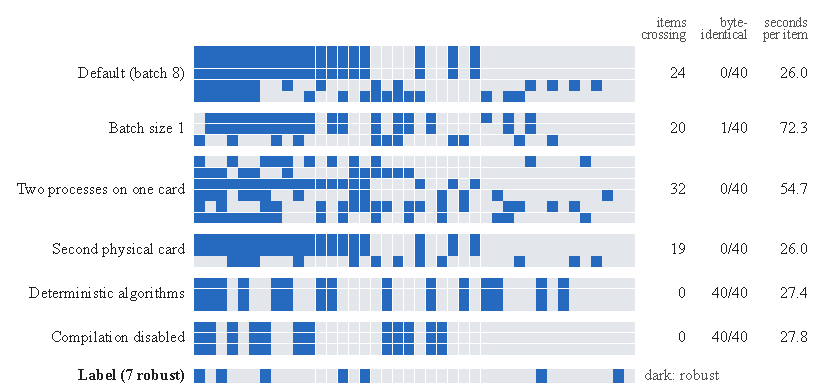
\includegraphics[width=\linewidth]{fig_rumore.pdf}
\caption{Predictions of the official pipeline for 40 preliminary public problems (columns) in 23 executions on DeepSeek (rows), by configuration; the last row is the label, dark cells are robust, and columns are sorted by how often they are predicted robust. At right: items whose prediction changes across the configuration's runs (more runs, more crossings), items whose generated text is byte-identical in all of them, and seconds per item.}
\label{fig:noise}
\end{figure}

\begin{table}[t]
\caption{Repeatability of the official pipeline on DeepSeek, 40 public problems, by configuration, in the order of Figure~\ref{fig:noise}. ``Crossings'': items whose prediction changes across the configuration's runs. ``Identical'': items whose generated text is byte-identical in all runs. Cost is runtime against the default configuration. Card 0 and card 1 are the two GPUs of the same machine. With two processes on one card, any five of its six runs give 29 to 31 crossings.}
\label{tab:reexec}
\centering
\small
\begin{tabular}{@{}lllllll@{}}
\toprule
\textbf{Configuration} & \textbf{Card} & \textbf{Runs} & \textbf{Crossings} & \textbf{Identical} & \textbf{Correct per run} & \textbf{Cost} \\
\midrule
Default (batch 8) & 0 & 5 & 24/40 & 0/40 & 24, 24, 24, 23, 24 & reference \\
Batch size 1 & 0 & 3 & 20/40 & 1/40 & 20, 21, 24 & +178\% \\
Two processes on one card & 0 & 6 & 32/40 & 0/40 & 24 to 28 & +110\% \\
Second physical card & 1 & 3 & 19/40 & 0/40 & 24, 24, 21 & +0\% \\
Deterministic algorithms & 0 & 3 & 0/40 & 40/40 & 24, 24, 24 & +5\% \\
Compilation disabled & 1 & 3 & 0/40 & 40/40 & 25, 25, 25 & +7\% \\
\bottomrule
\end{tabular}
\end{table}

\paragraph{Two candidate remedies.} Deterministic algorithms (PyTorch's, in warn-only mode, with deterministic cuDNN and a fixed cuBLAS workspace; Appendix~\ref{app:C}) and disabled compilation each made the generated text byte-identical in three sequential runs, at 5 to 7\% runtime cost. On card 0, the default configuration produced 24 crossings in five runs. Each remedy ran on one card where the default had produced crossings, each run in a new process, with no other process on that card. Three identical runs are weak evidence: the default configuration also gave three identical runs on card 0 before its fourth diverged, and five of its eight runs on the two cards shared one output. The two remedies produced different outputs, predicting 15 and 12 of the 40 problems robust, and because they ran on different cards we cannot tell whether the difference comes from the configuration or from the card. Neither gained more than one item (24 and 25 correct).

\paragraph{Distinct outputs.} The 23 executions fall into 14 distinct outputs, byte-identical within each. The same output appeared on both cards, and two runs launched in the same second on one card produced different outputs, so the output is not a property of the card alone; what selects it is not established. As only 7 of the 40 problems are robust and crossings largely cancel, accuracy moved much less than predictions: 21 to 24 correct in the default configuration on either card and 24 to 28 with two processes on one card, always below the 33 of the majority constant. An exploratory repetition of the official score extraction, whose third run ranks the 164 labeled problems at Spearman 0.24 against the first two, is in Appendix~\ref{app:C}.

\section{Regenerating the labels with our own protocol}\label{sec:labels}

\paragraph{Our labeling protocol.} We identified the organizers' perturbation families in the preliminary data (rephrase, rename, domain, distract, typos), regenerated them with gpt-oss-120b prompted with public examples, and gated each variant with gpt-oss-120b. An answer counts as correct when it matches gpt-oss-120b's answer on the original problem, because the preliminary data carry no answers; we did not check this key against the answers of the collections the problems come from. On the organizers' machine, with vLLM 0.28.0 [8] outside the official image, we labeled four models with two independent draws of variants (A and B, about 40 accepted variants per problem): 10 samples on the base problem and one per variant, at temperature 0.6, top-p 0.95 and at most 16,384 new tokens. Draw A's variants were also re-sampled with a new seed (A$'$). A label is robust when at least 6 of the 10 base samples are correct and every variant is answered correctly; unlike the earlier rule's conjunction, this requires the base problem to be solved.

A chain that reaches our cap is scored by the last boxed answer it contains, and counts as wrong without one; the organizers also count a response that reaches their limit without a parseable final answer as wrong [4]. Our protocol differs from the organizers' in perturbations, answer key, rule and sampling (one answer per variant, against 10 in the files behind most of their DeepSeek labels). Its decoding differs from the settings they publish, and its prompt may differ from the one behind their labels, which they have not stated.

\begin{table}[t]
\caption{Agreement of labels regenerated with our protocol: Cohen's kappa. The three columns for A and B treat variant chains that reached the 16,384-token cap in three ways: scored as in the protocol (by their last boxed answer, if any), dropped, or all counted as correct. The first of these columns and the A and A$'$ column give 95\% percentile bootstrap intervals over problems, and the script of Appendix~\ref{app:E} gives them for the other two. A problem has a label in a draw when it has at least one accepted variant (160 in A, 159 in B). Kappa between A and B uses the 159 problems labeled in both (150 for Qwen3.5-4B and 156 for DeepSeek when truncated chains are dropped), and between A and A$'$ 160. ``At cap'': percentage of variant chains that reached the cap in draws A and B. ``Robust'': percentage of problems labeled robust in draw A, as scored. The last column gives kappa of draw A with the organizers' preliminary DeepSeek labels: on the 138 published ones, and on the 160 that include 22 labels we derived (Section~\ref{sec:data}).}
\label{tab:label}
\centering
\small
\setlength{\tabcolsep}{3pt}
\begin{tabular}{@{}llllllll@{}}
\toprule
& & & \multicolumn{3}{l}{\textbf{A and B, truncated variant chains}} & & \\
\cmidrule(lr){4-6}
\textbf{Model} & \textbf{At cap} & \textbf{Robust} & \textbf{as scored} & \textbf{dropped} & \textbf{correct} & \textbf{A and A$'$} & \textbf{Organizers'} \\
\midrule
Skywork & 1.2, 1.5 & 74 & 0.44 [0.28, 0.59] & 0.39 & 0.39 & 0.79 [0.67, 0.89] & none \\
DeepSeek & 5.1, 6.1 & 39 & 0.41 [0.26, 0.55] & 0.35 & 0.36 & 0.46 [0.33, 0.59]$^{*}$ & 0.011; 0.025 \\
Olmo & 1.1, 0.9 & 68 & 0.38 [0.21, 0.54] & 0.39 & 0.39 & 0.65 [0.52, 0.78] & none \\
Qwen3.5-4B & 22.1, 29.2 & 9 & 0.18 [$-$0.06, 0.39] & 0.26 & 0.44 & not run & none \\
\bottomrule
\end{tabular}
\par\smallskip{\footnotesize $^{*}$On DeepSeek, A$'$ also received the answer-format line (end of this section), so this entry mixes seed and prompt.}
\end{table}

\paragraph{Results.} Under our protocol, two independent draws of variants give labels that agree at kappa 0.35 to 0.44 on Skywork, Olmo and DeepSeek, whether truncated variant chains are scored as in the protocol, dropped or all counted as correct (Table~\ref{tab:label}). On Qwen3.5-4B, 22 to 29\% of the variant chains reach the cap. Scoring these chains as in the protocol, dropping them or counting them all as correct gives agreement of 0.18, 0.26 and 0.44, and a robust share in draw A of 9\%, 83\% and 79\%. On Skywork, re-sampling the same variants with a new seed agrees far more than drawing new variants (0.79 against 0.44), so its label depends more on the variants than on the seed; on Olmo the gap is smaller (0.65 against 0.38), and on DeepSeek, where A$'$ also changed the prompt, it is 0.46 against 0.41.

Draw A's DeepSeek labels agree with the 138 labels the organizers published at kappa 0.011 [$-$0.13, 0.17], and with the 160 that include 22 of our derived labels at 0.025 [$-$0.12, 0.18]. Of the 36 problems with a published robust label, draw A calls 20 non-robust, and 4 of these change when truncated variants all count as correct. Of the 102 with a published non-robust label, draw A calls 44 robust. The reliability of the organizers' labels remains unmeasured. A retrospective calculation on the same saved answers with the main-phase threshold rule, applied as its pre-registration fixed it, with no filter on the base problem (Appendix~\ref{app:C}), gives test-retest point estimates between 0.34 and 0.56, below the pre-registered bar of 0.60, though three of the four intervals include it.

\paragraph{The prompt changes our labels.} In a first run with the bare problem text, later discarded, \mbox{Qwen3.5-4B} gave a final answer in the expected format in only 5 of its 1,640 base samples in draw A. With one instruction line requesting the format, 145 of 164 problems passed the base condition, against none. DeepSeek passed it on 147 of 164 with or without that line; its draws A and B ran without the line and A$'$ with it, and on the same variants its robust share moved from 39\% to 51\% of the 160 labeled problems, a change that mixes prompt and seed. Under our protocol, the label of Qwen3.5-4B therefore depends on the prompt. Whether this affects the organizers' labels is unknown: their baselines repository has a solve prompt that asks for an ANSWER line, but they have not said whether it was used for labeling (R3).

\section{The falsification campaign}\label{sec:campaign}

Table~\ref{tab:campaign} summarizes the campaign; Appendix~\ref{app:A} lists all 31 entries and explains three traps (rule T, the oracle H13, the duplicated pairs behind H2) and two pitfalls of the data. All entries use the preliminary data, except H16 to H18, which were scored on the 17 items of the warmup evaluation task.

\begin{table}[t]
\caption{The campaign in brief, in 19 of its 31 entries (Appendix~\ref{app:A} lists all). Ground truth is DeepSeek's and the preliminary pairs' unless stated; accuracy differences are in points against each pre-registration's baseline. H1, H7 and T count the 52 duplicated DeepSeek pairs twice; counted once, no verdict changes.}
\label{tab:campaign}
\centering
\small
\begin{tabular}{@{}L{5.5cm}L{1.9cm}L{5.6cm}@{}}
\toprule
\textbf{What we tested} & \textbf{Entries} & \textbf{Outcome} \\
\midrule
Text features; robustness as a property of the problem; labels, base accuracy and difficulty order across models & H1 to H5, H7 & rejected; H2 gained only when the duplicated pairs were counted twice \\
Official uncertainty features, logistic regression & H10 & 0.774 against a majority constant of 0.756, within the 0.692 $\pm$ 0.101 of the proposal [1] (method substituted) \\
Features cached for other models; per-target thresholds & H12, H13 & H12 rejected; the H13 ceiling withdrawn, $-$2.8 points when forced to rank \\
Our perturbation families, translation, self-consistency, the organizers' families regenerated (pilot), representation shift & H19, H22, H30 to H33 & rejected: kappa at most 0.02, AUROC at most 0.615 \\
Probes on DeepSeek's hidden states: ours and the organizers' published artifact & H36, H35 & survive their nulls; ours adds no detectable gain over length, and the artifact's score is probably in-sample \\
Trivial-robust rule, post hoc & T & a trap: +6.0 points on the preliminary pairs, +0.0 on \texttt{val-sample} \\
Identical bundles re-executed (warmup, 17 items) & H18 & noise confirmed: 11, 9, 11 and 11 correct \\
\bottomrule
\end{tabular}
\end{table}

\paragraph{Length and probes.} The character count of the problem alone orders the 164 DeepSeek labels at AUROC 0.704. Our logistic probe on DeepSeek's last-token hidden states, with layer and regularization chosen by inner cross-validation, reaches 0.710 out of fold with the original fold assignment. Over 20 other assignments, passed through the second-stage model below, it gives 0.57 to 0.76 (mean 0.69). Its scores correlate with length at Spearman +0.55, and residualized on log character count it gives 0.62. Its permutation null, rerun with 1{,}000 permutations of the whole nested procedure (the first version used 60, where 500 were pre-registered), gives $p = 0.002$. Restricted to the 138 published labels, these out-of-fold scores give 0.714 and length 0.733; retrained on those 138 alone with H36's procedure and seed, the probe gives 0.620. Combined with length in a second-stage model fitted on common outer folds, the probe changes AUROC over length alone by +0.005 on the 164 labels and by $-$0.010 on the 138 published ones (median bounds of the per-assignment 95\% intervals: $-$0.03 to 0.04, and $-$0.04 to 0.02): we detect no gain from adding the probe to length (Appendix~\ref{app:C}). This analysis replaces an earlier combination that leaked labels (Appendix~\ref{app:D}).

The organizers' published DeepSeek probe artifact orders the 164 DeepSeek labels at 0.739 with the aggregation we pre-registered and at 0.709 with its own, and at 0.62 and 0.57 residualized on log character count; its controls trained on shuffled labels give 0.68 at layer 31. The artifact does not record its training data; we infer that 137 of the 164 problems were among the public rows it was trained on, so these scores are probably largely in-sample. These length controls, which play the role of control tasks [7], were post hoc. Whether either probe reads anything beyond length that bears on robustness is not established. Apart from the three traps of Appendix~\ref{app:A}, no signal we scored by accuracy beats the majority constant by more than about one standard error on the preliminary labels, most of them DeepSeek's.

\section{Our entries}\label{sec:entries}

Our entry V8, pre-registered on 13 September, is the whole rule \texttt{return~[len(p)~>=~98 for~p~in~problems]}, with the threshold at the lower median of the 174 preliminary problems and the direction fixed on the preliminary pairs. On the original main-phase tasks it scored 11/21 and 10/19, like our entry v6 and the organizers' own entries. None of these beat the majority constant, which scores at least 11/21 and 10/19 on these tasks, and on so few items the ties do not show that length carries no signal (95\% Wilson intervals 0.32 to 0.72 and 0.32 to 0.73). On the 71 labeled rows of the official training set (revision of 17 September; 36 distinct problems), V8 differs from the all-robust constant on only 6 rows and is wrong on all 6 (46/71 against 52/71): too few to say what length is worth on official data. On the replacement tasks of 16 September, before and after the evaluation changed on 15 October [6], it predicted robust for every item (10/21 and 7/14), like an all-robust control. For the final test we nominated V8 (Codabench 1016713) and the constant (1016732), both on the Main track; our pre-registered predictions will be scored there (Appendix~\ref{app:B}).

\section{Recommendations}\label{sec:recs}

These rest mostly on DeepSeek and the preliminary data, and should be checked on the other models.
\begin{itemize}
\item \textbf{R1. Remove the variation between runs, and test the remedy:} on the same card with independent restarts, under load and across cards.
\item \textbf{R2. Repeat only where it decides something:} at the warmup's re-execution noise (a standard deviation of 1.0 item on 17, itself estimated from four runs), a one-item gap needs about eight runs per entry to reach two standard errors, so repeat only entries that run a model and sit near a prize boundary.
\item \textbf{R3. Say which prompt and decoding settings produced each released label file,} at least after the close.
\item \textbf{R4. Measure the label's reliability directly,} with two independent draws of variants labeled by the official process.
\item \textbf{R5. Show floors and noise on the leaderboard:} a row per constant predictor, the re-execution noise and binomial intervals.
\item \textbf{R6. Require a length control in white-box ablations.}
\item \textbf{R7. Remove the leaking field} \texttt{permutation\_type} from the aggregated datasets (Appendix~\ref{app:A}).
\end{itemize}

\paragraph{Code and data.} Our code, bundles, pre-registrations and outcome files are released at \href{https://github.com/Dan23RR/aimo-instrument}{\nolinkurl{github.com/Dan23RR/aimo-instrument}}. Its folder \texttt{reproduce/} recomputes the main tables from saved outputs and the six preliminary datasets, and the other numbers come from the dated records in \texttt{archive/} (Appendix~\ref{app:E}).

%%%%%% End of the main text: the six pages end here; the Limitations do not count %%%%%%
\label{fine-testo}

\section*{Limitations}

\begin{enumerate}[leftmargin=1.6em, itemsep=2pt, topsep=4pt, parsep=0pt]
\item \textbf{Preliminary data, not official data.} We did not repeat our label and probe analyses on the official training set, beyond the evaluation of V8 and a five-row check of our labels (Appendix~\ref{app:C}). Findings on label reliability and predictability may not generalize to the official evaluation setting.
\item \textbf{Our protocol, not the official one.} We did not regenerate labels with the organizers' published settings (100,000 tokens, temperature 1.0), with 10 answers per variant as in the files behind most DeepSeek labels, or on \texttt{train-main-v2}. The three treatments of truncated variant chains show how much our cap moves agreement between our draws; all three score base samples that reach the cap as the protocol does, and none of them reproduces longer decoding or a different temperature. Our low agreement with the organizers' labels is a fact about our process.
\item \textbf{One model.} We ran the probes, the re-execution study of Section~\ref{sec:reexec} and the comparisons of our regenerated labels with the organizers' preliminary labels only on DeepSeek.
\item \textbf{Re-execution.} We did not run the two candidate remedies on the same card, so card and configuration are confounded; we did not test either remedy under contention or on both cards, and we used 40 problems and one image.
\item \textbf{Records.} Some analyses rest on re-created scripts or dated records (Appendix~\ref{app:D}). Nothing here estimates performance on the final held-out problems.
\end{enumerate}

\section*{AI usage statement}

In this work, we used one generative AI tool, Claude (Anthropic), through Claude Code, for ideation, coding, analysis and writing. Ideation: it drafted the pre-registrations, including hypotheses, predictions and kill criteria, and searched and summarized the literature and the public records, including the organizers' Discord channels and the author's correspondence with them. Coding: it wrote the solution code of our bundles and the analysis and extraction scripts, ran them, and operated the organizers' virtual machine over SSH. Analysis: it computed and interpreted the results and ran automated adversarial reviews of hypotheses, drafts and code. Writing: it drafted the correspondence, this report and its revision after review.

It also made most of our Codabench uploads through the author's browser at the author's instruction. There were two exceptions: one resubmission (925822, 14 September), made without a specific instruction, and one submission that the author had not approved, sent in error and rejected before import (1016734, 28 October).

Language models were also components of our method: gpt-oss-120b generated and gated the perturbation variants and supplied the reference answers of Section~\ref{sec:labels}, and phi-4 translated problems for H22. The final decisions on the direction of the work, on the submissions (with the two exceptions above), on the nominations for the final test and on the claims of this report were the author's, and the author sent all correspondence personally. The author has reviewed all AI-assisted work and takes full responsibility for the final content of this report.

\begin{ack}
We thank Michal Štefánik, Róbert Belanec and the AIMO Interpretability team for the compute grant, a virtual machine with two GPUs, and for answering our questions; on 2 November they confirmed that the measurements taken on their machine may appear in this report. We also thank the three reviewers and the program chairs: two reviewers checked our analyses against the released code and data, and their checks corrected several of our claims. Other GPU time was rented on Modal and paid by the author or covered by Modal's platform credit. This work received no other funding, and the author has no competing interests.
\end{ack}

\section*{References}
{\small
[1] M. Štefánik, P. Mondorf, A. Waldis, Q. Liu, C. Yang, M. Spiegel, J. Kuchař, M. Kadlčík, A. Vawda-Oomerjee, C. Liu, S. Frieder, B. Plank, F. Barez and P. Stenetorp. AIMO Interpretability Challenge. CoRR, abs/2607.13899, 2026. doi:10.48550/arXiv.2607.13899.

[2] H. He and Thinking Machines Lab. Defeating Nondeterminism in LLM Inference. Thinking Machines Lab: Connectionism, 2025.

[3] J. Yuan, H. Li, X. Ding, W. Xie, Y.-J. Li, W. Zhao, K. Wan, J. Shi, X. Hu and Z. Liu. Understanding and Mitigating Numerical Sources of Nondeterminism in LLM Inference. NeurIPS 2025. arXiv:2506.09501.

[4] AIMO Interpretability Challenge website and FAQ. \url{https://aimo-interp.github.io} (accessed 28 October 2026), and its source repository aimo-interp/aimo-interp.github.io on GitHub.

[5] aimo-interp/getting-started and aimo-interp/baselines, GitHub repositories: README and issues \#6 and \#10 of getting-started; aimo-interp datasets on Hugging Face, including \texttt{train-main-v2} and \texttt{val-sample}.

[6] AIMO Interpretability Challenge Discord, \#announcements and \#qa: 5, 15 and 22 September, 9, 15, 16 and 20 October 2026.

[7] J. Hewitt and P. Liang. Designing and Interpreting Probes with Control Tasks. EMNLP-IJCNLP 2019.

[8] W. Kwon et al. Efficient Memory Management for Large Language Model Serving with PagedAttention. SOSP 2023.

[9] D. Hendrycks et al. Measuring Mathematical Problem Solving With the MATH Dataset. NeurIPS 2021 Datasets and Benchmarks Track. arXiv:2103.03874.
}

%%%%%% End of the references %%%%%%
\clearpage
\appendix
\raggedright

\input{app_A}
\input{app_B}
\input{app_C}
\input{app_D}
\input{app_E}

\newpage
\input{checklist_compilata.tex}

\end{document}
".
%% Every line numbered (same numbering, used to find the lines cited in the note): "\def\everyline{}\documentclass{article}

%% Conditional revision of November 2026: six pages of main text, from the title to the end of Section 7 (label
%% fine-testo); the Limitations, the AI usage statement, the references and the appendices do not count.
%% Final mode with the workshop name. Line numbers on every fifth line, small and grey, for the note to the
%% program chairs, who asked for section and line numbers. Copy without them: pdflatex "\def\cleancopy{}\input{main}".
%% Every line numbered (same numbering, used to find the lines cited in the note): "\def\everyline{}\input{main}".
\usepackage[final,sglblindworkshop]{neurips_2026}
\workshoptitle{AIMO Interpretability Challenge}
\ifdefined\cleancopy\else
  \usepackage{lineno}
  \linenumbers
  \ifdefined\everyline\else\modulolinenumbers[5]\fi
  \renewcommand\linenumberfont{\normalfont\tiny\sffamily\color{black!45}}
\fi

\usepackage[utf8]{inputenc}
\usepackage[T1]{fontenc}
%% Typewriter text in Latin Modern, the Type 1 version of the default Computer Modern typewriter, with the same
%% widths: without it, \texttt in T1 encoding becomes bitmap (Type 3) fonts, and the template asks for Type 1 fonts.
\renewcommand{\ttdefault}{lmtt}
\usepackage{hyperref}
\hypersetup{pdftitle={The Instrument Behind the Leaderboard: Re-Execution Noise and Label Regeneration in the AIMO Interpretability Challenge}, pdfauthor={Daniel Culotta}}
\usepackage{url}
\def\UrlBreaks{\do\/\do\.\do\_\do\-\do\:}
\usepackage{booktabs}
\usepackage{array}
\usepackage{longtable}
\newcolumntype{L}[1]{>{\raggedright\arraybackslash}p{#1}}
\usepackage{amsfonts}
\usepackage{microtype}
\usepackage{xcolor}
\usepackage{graphicx}
\usepackage{enumitem}
\usepackage{needspace}
\setlist[itemize]{leftmargin=1.4em, itemsep=2pt, topsep=4pt, parsep=0pt}
\setlist[itemize,2]{label=$\circ$}
\renewcommand{\arraystretch}{1.15}
\raggedbottom

\title{The Instrument Behind the Leaderboard: Re-Execution Noise and Label Regeneration in the AIMO Interpretability Challenge}

\author{%
  Daniel Culotta \\
  Independent researcher
}

\begin{document}

\maketitle

\begin{abstract}
We treat the AIMO Interpretability benchmark, which asks whether a model's answer to a math problem survives perturbations, as a measurement instrument. Almost all our label and probe analyses use the preliminary datasets. As the program chairs note, these differ from the official training and validation data in sampling, perturbations and eligibility, so findings on label reliability and predictability may not hold in the official evaluation. First, on DeepSeek-R1-0528-Qwen3-8B in the official pipeline, 24 of 40 items changed prediction across five default runs. Turning compilation off, or deterministic algorithms on, gave three byte-identical runs, each on one card. Second, we regenerated labels with our own protocol, not the official one: our perturbations and answer key, one answer per variant, a 16,384-token cap and temperature 0.6, where the organizers publish 100,000 tokens and 1.0. Two independent draws agree at kappa 0.35 to 0.44 on three of four models however truncated chains are treated, and 0.18 to 0.44 on Qwen3.5-4B, whose chains often reach the cap. Draw A agrees with the 138 published DeepSeek labels at kappa 0.01. This describes our protocol and does not measure the reliability of the organizers' labels. Third, of the 27 dated hypotheses with a kill criterion, 21 failed it. Our probe on DeepSeek's hidden states does no better than problem length (AUROC 0.710 against 0.704; below length on the published labels) and adds nothing detectable to it.
\end{abstract}

\section{Introduction}\label{sec:1}

A leaderboard is a measurement. Its score is read off an instrument made of a label, an evaluation set, an inference pipeline and the hardware it runs on. When the label is itself produced by a stochastic process, the instrument has noise of its own, which a single submission cannot see. We measure the re-execution noise of the official extraction and regressor, and the repeatability of labels regenerated with our own protocol, not the noise of the organizers' labels.

We study the instrument of the AIMO Interpretability Challenge, in which a submission predicts, for a given model and math problem, whether the model's answer is robust to perturbations of the problem [1]. We ran our work as a falsification campaign: every hypothesis was recorded in a dated file, 26 of the 31 before their data were seen, and every tested hypothesis is reported. Of the 31 entries, 27 carried a kill criterion written before their test ran (for 3 of them in a written plan rather than a frozen pre-registration, and for H2 after its concordance had been seen). By that criterion 21 were rejected, 5 survived and 1 is not established (Appendix~\ref{app:A}).

\paragraph{Scope.} Three limits apply.
\begin{itemize}
\item \textbf{Preliminary and official data.} Almost all of our label and probe analyses use the six preliminary public datasets released before the main phase. Their labels follow an earlier rule than those of the official training set (\texttt{train-main-v2}) and of the validation and test tasks [5]; as the program chairs noted in their meta-review, their sampling procedures, perturbations and eligibility criteria also differ. Beyond the label rule, we did not compare the two. Unless we say otherwise, a result on labels or on their predictability holds for the preliminary data and may not hold in the official evaluation setting.
\item \textbf{Our labeling protocol is not the official one.} When we regenerate labels (Section~\ref{sec:labels}), we use our own perturbations, prompts, sampling, decoding, answer key and labeling rule. Disagreement with the organizers' preliminary labels therefore shows that the two processes give different labels; it does not establish that their labels are unreliable or irreproducible.
\item \textbf{Mostly one model.} The re-execution study of Section~\ref{sec:reexec}, the probe analyses and every comparison of our regenerated labels with the organizers' preliminary labels are on DeepSeek-R1-0528-Qwen3-8B. Regenerated labels cover four models, but no conclusion about the official benchmark is established across models.
\end{itemize}

Within these limits, Sections~\ref{sec:reexec} to~\ref{sec:campaign} report re-execution noise and two candidate remedies, our regenerated labels, and signals that do no better than problem length or come from an artifact of the data. Nondeterminism of LLM inference is documented in general [2, 3]; we add its size for one model, one submission and 40 problems on this benchmark's hardware and pipeline. We make no claim about any participant's method.

\section{The task, the labels and the data}\label{sec:data}

\paragraph{Task.} A submission receives a model identifier, a reasoning effort and a list of problems, and returns one robustness verdict per problem, offline on one GPU within one hour [4, 5], or 70 minutes since 15 October [6]. The models are Qwen3.5-4B, Skywork-OR1-Math-7B, Olmo-3-7B-Think and \mbox{DeepSeek-R1-0528-Qwen3-8B} in both tracks, and gpt-oss-120b in the Main track only.

\paragraph{Official data.} The main-phase training set \texttt{train-main-v2} labels all five models with a threshold on the largest accuracy drop across perturbation families: robust at most 0.10, non-robust at least 0.25, no label in between [5]. The organizers' published decoding settings are up to 100,000 tokens at temperature 1.0, top-k 40 and top-p 0.95, and a response that reaches the limit without a final answer counts as wrong [4]. Since 16 September the private validation tasks have 21 items (Main) and 14 (Small), on which the binomial standard error of an accuracy near one half is 10.9 and 13.4 points; the final test uses 30 to 50 new problems [5, 6].

\paragraph{Preliminary data.} Six datasets released before the main phase aggregate to 335 (model, problem) pairs over 174 distinct problems, up to eight per problem; 52 pairs repeat the DeepSeek measurements under a second model name. Their labels follow an earlier rule: on all 379 labeled rows (a pair can have several), the label equals the conjunction ``no perturbation lowered accuracy''. A per-family majority rule (``more than half of the answers are correct in every perturbation family'') reproduces the same 379 labels, so these rows cannot tell the two rules apart. Whether they used the decoding settings above is not documented; in the files behind most DeepSeek labels, most variants listed as lowering accuracy were answered 10 times. We call their labels the organizers' preliminary labels, and keep ``official'' for \texttt{train-main-v2} and the validation and test tasks.

\paragraph{DeepSeek labels.} DeepSeek is the only evaluated model with many preliminary labels: 164 distinct problems (the 52 duplicated pairs count once). For 138 of them the data publish a label. For the other 26 we derived one with the conjunction, which makes 4 of them robust; the majority rule would make 21 robust, so these 26 labels depend on the choice of rule. We therefore report results on the 138 published labels separately.

\section{Re-execution noise on the evaluation workers' type of GPU}\label{sec:reexec}

On a virtual machine lent by the organizers, with two NVIDIA RTX PRO 6000 Blackwell Server Edition GPUs (the type the evaluation workers use), we ran 40 preliminary public problems through the official runtime image, extraction and regressor, unmodified, on DeepSeek. Decoding was greedy, with at most 4,096 new tokens in batches of 8. The 40 labels are DeepSeek's of Section~\ref{sec:data}: 28 published and 12 that we derived with the conjunction, which include 3 of the 7 robust ones. Figure~\ref{fig:noise} shows the 23 executions; Table~\ref{tab:reexec} gives the repeatability of each configuration.

\begin{figure}[t]
\centering
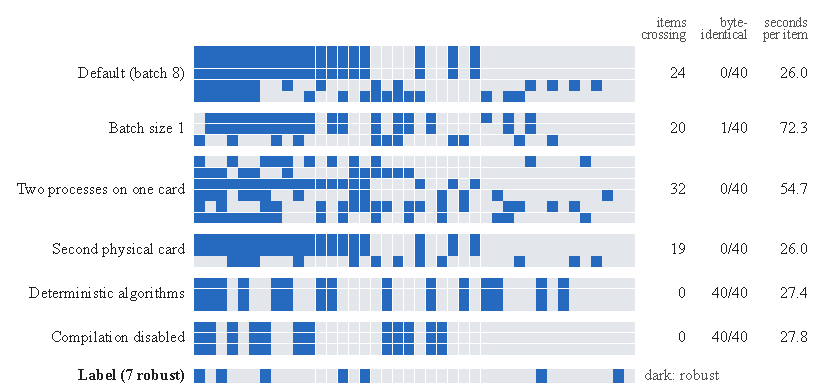
\includegraphics[width=\linewidth]{fig_rumore.pdf}
\caption{Predictions of the official pipeline for 40 preliminary public problems (columns) in 23 executions on DeepSeek (rows), by configuration; the last row is the label, dark cells are robust, and columns are sorted by how often they are predicted robust. At right: items whose prediction changes across the configuration's runs (more runs, more crossings), items whose generated text is byte-identical in all of them, and seconds per item.}
\label{fig:noise}
\end{figure}

\begin{table}[t]
\caption{Repeatability of the official pipeline on DeepSeek, 40 public problems, by configuration, in the order of Figure~\ref{fig:noise}. ``Crossings'': items whose prediction changes across the configuration's runs. ``Identical'': items whose generated text is byte-identical in all runs. Cost is runtime against the default configuration. Card 0 and card 1 are the two GPUs of the same machine. With two processes on one card, any five of its six runs give 29 to 31 crossings.}
\label{tab:reexec}
\centering
\small
\begin{tabular}{@{}lllllll@{}}
\toprule
\textbf{Configuration} & \textbf{Card} & \textbf{Runs} & \textbf{Crossings} & \textbf{Identical} & \textbf{Correct per run} & \textbf{Cost} \\
\midrule
Default (batch 8) & 0 & 5 & 24/40 & 0/40 & 24, 24, 24, 23, 24 & reference \\
Batch size 1 & 0 & 3 & 20/40 & 1/40 & 20, 21, 24 & +178\% \\
Two processes on one card & 0 & 6 & 32/40 & 0/40 & 24 to 28 & +110\% \\
Second physical card & 1 & 3 & 19/40 & 0/40 & 24, 24, 21 & +0\% \\
Deterministic algorithms & 0 & 3 & 0/40 & 40/40 & 24, 24, 24 & +5\% \\
Compilation disabled & 1 & 3 & 0/40 & 40/40 & 25, 25, 25 & +7\% \\
\bottomrule
\end{tabular}
\end{table}

\paragraph{Two candidate remedies.} Deterministic algorithms (PyTorch's, in warn-only mode, with deterministic cuDNN and a fixed cuBLAS workspace; Appendix~\ref{app:C}) and disabled compilation each made the generated text byte-identical in three sequential runs, at 5 to 7\% runtime cost. On card 0, the default configuration produced 24 crossings in five runs. Each remedy ran on one card where the default had produced crossings, each run in a new process, with no other process on that card. Three identical runs are weak evidence: the default configuration also gave three identical runs on card 0 before its fourth diverged, and five of its eight runs on the two cards shared one output. The two remedies produced different outputs, predicting 15 and 12 of the 40 problems robust, and because they ran on different cards we cannot tell whether the difference comes from the configuration or from the card. Neither gained more than one item (24 and 25 correct).

\paragraph{Distinct outputs.} The 23 executions fall into 14 distinct outputs, byte-identical within each. The same output appeared on both cards, and two runs launched in the same second on one card produced different outputs, so the output is not a property of the card alone; what selects it is not established. As only 7 of the 40 problems are robust and crossings largely cancel, accuracy moved much less than predictions: 21 to 24 correct in the default configuration on either card and 24 to 28 with two processes on one card, always below the 33 of the majority constant. An exploratory repetition of the official score extraction, whose third run ranks the 164 labeled problems at Spearman 0.24 against the first two, is in Appendix~\ref{app:C}.

\section{Regenerating the labels with our own protocol}\label{sec:labels}

\paragraph{Our labeling protocol.} We identified the organizers' perturbation families in the preliminary data (rephrase, rename, domain, distract, typos), regenerated them with gpt-oss-120b prompted with public examples, and gated each variant with gpt-oss-120b. An answer counts as correct when it matches gpt-oss-120b's answer on the original problem, because the preliminary data carry no answers; we did not check this key against the answers of the collections the problems come from. On the organizers' machine, with vLLM 0.28.0 [8] outside the official image, we labeled four models with two independent draws of variants (A and B, about 40 accepted variants per problem): 10 samples on the base problem and one per variant, at temperature 0.6, top-p 0.95 and at most 16,384 new tokens. Draw A's variants were also re-sampled with a new seed (A$'$). A label is robust when at least 6 of the 10 base samples are correct and every variant is answered correctly; unlike the earlier rule's conjunction, this requires the base problem to be solved.

A chain that reaches our cap is scored by the last boxed answer it contains, and counts as wrong without one; the organizers also count a response that reaches their limit without a parseable final answer as wrong [4]. Our protocol differs from the organizers' in perturbations, answer key, rule and sampling (one answer per variant, against 10 in the files behind most of their DeepSeek labels). Its decoding differs from the settings they publish, and its prompt may differ from the one behind their labels, which they have not stated.

\begin{table}[t]
\caption{Agreement of labels regenerated with our protocol: Cohen's kappa. The three columns for A and B treat variant chains that reached the 16,384-token cap in three ways: scored as in the protocol (by their last boxed answer, if any), dropped, or all counted as correct. The first of these columns and the A and A$'$ column give 95\% percentile bootstrap intervals over problems, and the script of Appendix~\ref{app:E} gives them for the other two. A problem has a label in a draw when it has at least one accepted variant (160 in A, 159 in B). Kappa between A and B uses the 159 problems labeled in both (150 for Qwen3.5-4B and 156 for DeepSeek when truncated chains are dropped), and between A and A$'$ 160. ``At cap'': percentage of variant chains that reached the cap in draws A and B. ``Robust'': percentage of problems labeled robust in draw A, as scored. The last column gives kappa of draw A with the organizers' preliminary DeepSeek labels: on the 138 published ones, and on the 160 that include 22 labels we derived (Section~\ref{sec:data}).}
\label{tab:label}
\centering
\small
\setlength{\tabcolsep}{3pt}
\begin{tabular}{@{}llllllll@{}}
\toprule
& & & \multicolumn{3}{l}{\textbf{A and B, truncated variant chains}} & & \\
\cmidrule(lr){4-6}
\textbf{Model} & \textbf{At cap} & \textbf{Robust} & \textbf{as scored} & \textbf{dropped} & \textbf{correct} & \textbf{A and A$'$} & \textbf{Organizers'} \\
\midrule
Skywork & 1.2, 1.5 & 74 & 0.44 [0.28, 0.59] & 0.39 & 0.39 & 0.79 [0.67, 0.89] & none \\
DeepSeek & 5.1, 6.1 & 39 & 0.41 [0.26, 0.55] & 0.35 & 0.36 & 0.46 [0.33, 0.59]$^{*}$ & 0.011; 0.025 \\
Olmo & 1.1, 0.9 & 68 & 0.38 [0.21, 0.54] & 0.39 & 0.39 & 0.65 [0.52, 0.78] & none \\
Qwen3.5-4B & 22.1, 29.2 & 9 & 0.18 [$-$0.06, 0.39] & 0.26 & 0.44 & not run & none \\
\bottomrule
\end{tabular}
\par\smallskip{\footnotesize $^{*}$On DeepSeek, A$'$ also received the answer-format line (end of this section), so this entry mixes seed and prompt.}
\end{table}

\paragraph{Results.} Under our protocol, two independent draws of variants give labels that agree at kappa 0.35 to 0.44 on Skywork, Olmo and DeepSeek, whether truncated variant chains are scored as in the protocol, dropped or all counted as correct (Table~\ref{tab:label}). On Qwen3.5-4B, 22 to 29\% of the variant chains reach the cap. Scoring these chains as in the protocol, dropping them or counting them all as correct gives agreement of 0.18, 0.26 and 0.44, and a robust share in draw A of 9\%, 83\% and 79\%. On Skywork, re-sampling the same variants with a new seed agrees far more than drawing new variants (0.79 against 0.44), so its label depends more on the variants than on the seed; on Olmo the gap is smaller (0.65 against 0.38), and on DeepSeek, where A$'$ also changed the prompt, it is 0.46 against 0.41.

Draw A's DeepSeek labels agree with the 138 labels the organizers published at kappa 0.011 [$-$0.13, 0.17], and with the 160 that include 22 of our derived labels at 0.025 [$-$0.12, 0.18]. Of the 36 problems with a published robust label, draw A calls 20 non-robust, and 4 of these change when truncated variants all count as correct. Of the 102 with a published non-robust label, draw A calls 44 robust. The reliability of the organizers' labels remains unmeasured. A retrospective calculation on the same saved answers with the main-phase threshold rule, applied as its pre-registration fixed it, with no filter on the base problem (Appendix~\ref{app:C}), gives test-retest point estimates between 0.34 and 0.56, below the pre-registered bar of 0.60, though three of the four intervals include it.

\paragraph{The prompt changes our labels.} In a first run with the bare problem text, later discarded, \mbox{Qwen3.5-4B} gave a final answer in the expected format in only 5 of its 1,640 base samples in draw A. With one instruction line requesting the format, 145 of 164 problems passed the base condition, against none. DeepSeek passed it on 147 of 164 with or without that line; its draws A and B ran without the line and A$'$ with it, and on the same variants its robust share moved from 39\% to 51\% of the 160 labeled problems, a change that mixes prompt and seed. Under our protocol, the label of Qwen3.5-4B therefore depends on the prompt. Whether this affects the organizers' labels is unknown: their baselines repository has a solve prompt that asks for an ANSWER line, but they have not said whether it was used for labeling (R3).

\section{The falsification campaign}\label{sec:campaign}

Table~\ref{tab:campaign} summarizes the campaign; Appendix~\ref{app:A} lists all 31 entries and explains three traps (rule T, the oracle H13, the duplicated pairs behind H2) and two pitfalls of the data. All entries use the preliminary data, except H16 to H18, which were scored on the 17 items of the warmup evaluation task.

\begin{table}[t]
\caption{The campaign in brief, in 19 of its 31 entries (Appendix~\ref{app:A} lists all). Ground truth is DeepSeek's and the preliminary pairs' unless stated; accuracy differences are in points against each pre-registration's baseline. H1, H7 and T count the 52 duplicated DeepSeek pairs twice; counted once, no verdict changes.}
\label{tab:campaign}
\centering
\small
\begin{tabular}{@{}L{5.5cm}L{1.9cm}L{5.6cm}@{}}
\toprule
\textbf{What we tested} & \textbf{Entries} & \textbf{Outcome} \\
\midrule
Text features; robustness as a property of the problem; labels, base accuracy and difficulty order across models & H1 to H5, H7 & rejected; H2 gained only when the duplicated pairs were counted twice \\
Official uncertainty features, logistic regression & H10 & 0.774 against a majority constant of 0.756, within the 0.692 $\pm$ 0.101 of the proposal [1] (method substituted) \\
Features cached for other models; per-target thresholds & H12, H13 & H12 rejected; the H13 ceiling withdrawn, $-$2.8 points when forced to rank \\
Our perturbation families, translation, self-consistency, the organizers' families regenerated (pilot), representation shift & H19, H22, H30 to H33 & rejected: kappa at most 0.02, AUROC at most 0.615 \\
Probes on DeepSeek's hidden states: ours and the organizers' published artifact & H36, H35 & survive their nulls; ours adds no detectable gain over length, and the artifact's score is probably in-sample \\
Trivial-robust rule, post hoc & T & a trap: +6.0 points on the preliminary pairs, +0.0 on \texttt{val-sample} \\
Identical bundles re-executed (warmup, 17 items) & H18 & noise confirmed: 11, 9, 11 and 11 correct \\
\bottomrule
\end{tabular}
\end{table}

\paragraph{Length and probes.} The character count of the problem alone orders the 164 DeepSeek labels at AUROC 0.704. Our logistic probe on DeepSeek's last-token hidden states, with layer and regularization chosen by inner cross-validation, reaches 0.710 out of fold with the original fold assignment. Over 20 other assignments, passed through the second-stage model below, it gives 0.57 to 0.76 (mean 0.69). Its scores correlate with length at Spearman +0.55, and residualized on log character count it gives 0.62. Its permutation null, rerun with 1{,}000 permutations of the whole nested procedure (the first version used 60, where 500 were pre-registered), gives $p = 0.002$. Restricted to the 138 published labels, these out-of-fold scores give 0.714 and length 0.733; retrained on those 138 alone with H36's procedure and seed, the probe gives 0.620. Combined with length in a second-stage model fitted on common outer folds, the probe changes AUROC over length alone by +0.005 on the 164 labels and by $-$0.010 on the 138 published ones (median bounds of the per-assignment 95\% intervals: $-$0.03 to 0.04, and $-$0.04 to 0.02): we detect no gain from adding the probe to length (Appendix~\ref{app:C}). This analysis replaces an earlier combination that leaked labels (Appendix~\ref{app:D}).

The organizers' published DeepSeek probe artifact orders the 164 DeepSeek labels at 0.739 with the aggregation we pre-registered and at 0.709 with its own, and at 0.62 and 0.57 residualized on log character count; its controls trained on shuffled labels give 0.68 at layer 31. The artifact does not record its training data; we infer that 137 of the 164 problems were among the public rows it was trained on, so these scores are probably largely in-sample. These length controls, which play the role of control tasks [7], were post hoc. Whether either probe reads anything beyond length that bears on robustness is not established. Apart from the three traps of Appendix~\ref{app:A}, no signal we scored by accuracy beats the majority constant by more than about one standard error on the preliminary labels, most of them DeepSeek's.

\section{Our entries}\label{sec:entries}

Our entry V8, pre-registered on 13 September, is the whole rule \texttt{return~[len(p)~>=~98 for~p~in~problems]}, with the threshold at the lower median of the 174 preliminary problems and the direction fixed on the preliminary pairs. On the original main-phase tasks it scored 11/21 and 10/19, like our entry v6 and the organizers' own entries. None of these beat the majority constant, which scores at least 11/21 and 10/19 on these tasks, and on so few items the ties do not show that length carries no signal (95\% Wilson intervals 0.32 to 0.72 and 0.32 to 0.73). On the 71 labeled rows of the official training set (revision of 17 September; 36 distinct problems), V8 differs from the all-robust constant on only 6 rows and is wrong on all 6 (46/71 against 52/71): too few to say what length is worth on official data. On the replacement tasks of 16 September, before and after the evaluation changed on 15 October [6], it predicted robust for every item (10/21 and 7/14), like an all-robust control. For the final test we nominated V8 (Codabench 1016713) and the constant (1016732), both on the Main track; our pre-registered predictions will be scored there (Appendix~\ref{app:B}).

\section{Recommendations}\label{sec:recs}

These rest mostly on DeepSeek and the preliminary data, and should be checked on the other models.
\begin{itemize}
\item \textbf{R1. Remove the variation between runs, and test the remedy:} on the same card with independent restarts, under load and across cards.
\item \textbf{R2. Repeat only where it decides something:} at the warmup's re-execution noise (a standard deviation of 1.0 item on 17, itself estimated from four runs), a one-item gap needs about eight runs per entry to reach two standard errors, so repeat only entries that run a model and sit near a prize boundary.
\item \textbf{R3. Say which prompt and decoding settings produced each released label file,} at least after the close.
\item \textbf{R4. Measure the label's reliability directly,} with two independent draws of variants labeled by the official process.
\item \textbf{R5. Show floors and noise on the leaderboard:} a row per constant predictor, the re-execution noise and binomial intervals.
\item \textbf{R6. Require a length control in white-box ablations.}
\item \textbf{R7. Remove the leaking field} \texttt{permutation\_type} from the aggregated datasets (Appendix~\ref{app:A}).
\end{itemize}

\paragraph{Code and data.} Our code, bundles, pre-registrations and outcome files are released at \href{https://github.com/Dan23RR/aimo-instrument}{\nolinkurl{github.com/Dan23RR/aimo-instrument}}. Its folder \texttt{reproduce/} recomputes the main tables from saved outputs and the six preliminary datasets, and the other numbers come from the dated records in \texttt{archive/} (Appendix~\ref{app:E}).

%%%%%% End of the main text: the six pages end here; the Limitations do not count %%%%%%
\label{fine-testo}

\section*{Limitations}

\begin{enumerate}[leftmargin=1.6em, itemsep=2pt, topsep=4pt, parsep=0pt]
\item \textbf{Preliminary data, not official data.} We did not repeat our label and probe analyses on the official training set, beyond the evaluation of V8 and a five-row check of our labels (Appendix~\ref{app:C}). Findings on label reliability and predictability may not generalize to the official evaluation setting.
\item \textbf{Our protocol, not the official one.} We did not regenerate labels with the organizers' published settings (100,000 tokens, temperature 1.0), with 10 answers per variant as in the files behind most DeepSeek labels, or on \texttt{train-main-v2}. The three treatments of truncated variant chains show how much our cap moves agreement between our draws; all three score base samples that reach the cap as the protocol does, and none of them reproduces longer decoding or a different temperature. Our low agreement with the organizers' labels is a fact about our process.
\item \textbf{One model.} We ran the probes, the re-execution study of Section~\ref{sec:reexec} and the comparisons of our regenerated labels with the organizers' preliminary labels only on DeepSeek.
\item \textbf{Re-execution.} We did not run the two candidate remedies on the same card, so card and configuration are confounded; we did not test either remedy under contention or on both cards, and we used 40 problems and one image.
\item \textbf{Records.} Some analyses rest on re-created scripts or dated records (Appendix~\ref{app:D}). Nothing here estimates performance on the final held-out problems.
\end{enumerate}

\section*{AI usage statement}

In this work, we used one generative AI tool, Claude (Anthropic), through Claude Code, for ideation, coding, analysis and writing. Ideation: it drafted the pre-registrations, including hypotheses, predictions and kill criteria, and searched and summarized the literature and the public records, including the organizers' Discord channels and the author's correspondence with them. Coding: it wrote the solution code of our bundles and the analysis and extraction scripts, ran them, and operated the organizers' virtual machine over SSH. Analysis: it computed and interpreted the results and ran automated adversarial reviews of hypotheses, drafts and code. Writing: it drafted the correspondence, this report and its revision after review.

It also made most of our Codabench uploads through the author's browser at the author's instruction. There were two exceptions: one resubmission (925822, 14 September), made without a specific instruction, and one submission that the author had not approved, sent in error and rejected before import (1016734, 28 October).

Language models were also components of our method: gpt-oss-120b generated and gated the perturbation variants and supplied the reference answers of Section~\ref{sec:labels}, and phi-4 translated problems for H22. The final decisions on the direction of the work, on the submissions (with the two exceptions above), on the nominations for the final test and on the claims of this report were the author's, and the author sent all correspondence personally. The author has reviewed all AI-assisted work and takes full responsibility for the final content of this report.

\begin{ack}
We thank Michal Štefánik, Róbert Belanec and the AIMO Interpretability team for the compute grant, a virtual machine with two GPUs, and for answering our questions; on 2 November they confirmed that the measurements taken on their machine may appear in this report. We also thank the three reviewers and the program chairs: two reviewers checked our analyses against the released code and data, and their checks corrected several of our claims. Other GPU time was rented on Modal and paid by the author or covered by Modal's platform credit. This work received no other funding, and the author has no competing interests.
\end{ack}

\section*{References}
{\small
[1] M. Štefánik, P. Mondorf, A. Waldis, Q. Liu, C. Yang, M. Spiegel, J. Kuchař, M. Kadlčík, A. Vawda-Oomerjee, C. Liu, S. Frieder, B. Plank, F. Barez and P. Stenetorp. AIMO Interpretability Challenge. CoRR, abs/2607.13899, 2026. doi:10.48550/arXiv.2607.13899.

[2] H. He and Thinking Machines Lab. Defeating Nondeterminism in LLM Inference. Thinking Machines Lab: Connectionism, 2025.

[3] J. Yuan, H. Li, X. Ding, W. Xie, Y.-J. Li, W. Zhao, K. Wan, J. Shi, X. Hu and Z. Liu. Understanding and Mitigating Numerical Sources of Nondeterminism in LLM Inference. NeurIPS 2025. arXiv:2506.09501.

[4] AIMO Interpretability Challenge website and FAQ. \url{https://aimo-interp.github.io} (accessed 28 October 2026), and its source repository aimo-interp/aimo-interp.github.io on GitHub.

[5] aimo-interp/getting-started and aimo-interp/baselines, GitHub repositories: README and issues \#6 and \#10 of getting-started; aimo-interp datasets on Hugging Face, including \texttt{train-main-v2} and \texttt{val-sample}.

[6] AIMO Interpretability Challenge Discord, \#announcements and \#qa: 5, 15 and 22 September, 9, 15, 16 and 20 October 2026.

[7] J. Hewitt and P. Liang. Designing and Interpreting Probes with Control Tasks. EMNLP-IJCNLP 2019.

[8] W. Kwon et al. Efficient Memory Management for Large Language Model Serving with PagedAttention. SOSP 2023.

[9] D. Hendrycks et al. Measuring Mathematical Problem Solving With the MATH Dataset. NeurIPS 2021 Datasets and Benchmarks Track. arXiv:2103.03874.
}

%%%%%% End of the references %%%%%%
\clearpage
\appendix
\raggedright

\input{app_A}
\input{app_B}
\input{app_C}
\input{app_D}
\input{app_E}

\newpage
\input{checklist_compilata.tex}

\end{document}
".
\usepackage[final,sglblindworkshop]{neurips_2026}
\workshoptitle{AIMO Interpretability Challenge}
\ifdefined\cleancopy\else
  \usepackage{lineno}
  \linenumbers
  \ifdefined\everyline\else\modulolinenumbers[5]\fi
  \renewcommand\linenumberfont{\normalfont\tiny\sffamily\color{black!45}}
\fi

\usepackage[utf8]{inputenc}
\usepackage[T1]{fontenc}
%% Typewriter text in Latin Modern, the Type 1 version of the default Computer Modern typewriter, with the same
%% widths: without it, \texttt in T1 encoding becomes bitmap (Type 3) fonts, and the template asks for Type 1 fonts.
\renewcommand{\ttdefault}{lmtt}
\usepackage{hyperref}
\hypersetup{pdftitle={The Instrument Behind the Leaderboard: Re-Execution Noise and Label Regeneration in the AIMO Interpretability Challenge}, pdfauthor={Daniel Culotta}}
\usepackage{url}
\def\UrlBreaks{\do\/\do\.\do\_\do\-\do\:}
\usepackage{booktabs}
\usepackage{array}
\usepackage{longtable}
\newcolumntype{L}[1]{>{\raggedright\arraybackslash}p{#1}}
\usepackage{amsfonts}
\usepackage{microtype}
\usepackage{xcolor}
\usepackage{graphicx}
\usepackage{enumitem}
\usepackage{needspace}
\setlist[itemize]{leftmargin=1.4em, itemsep=2pt, topsep=4pt, parsep=0pt}
\setlist[itemize,2]{label=$\circ$}
\renewcommand{\arraystretch}{1.15}
\raggedbottom

\title{The Instrument Behind the Leaderboard: Re-Execution Noise and Label Regeneration in the AIMO Interpretability Challenge}

\author{%
  Daniel Culotta \\
  Independent researcher
}

\begin{document}

\maketitle

\begin{abstract}
We treat the AIMO Interpretability benchmark, which asks whether a model's answer to a math problem survives perturbations, as a measurement instrument. Almost all our label and probe analyses use the preliminary datasets. As the program chairs note, these differ from the official training and validation data in sampling, perturbations and eligibility, so findings on label reliability and predictability may not hold in the official evaluation. First, on DeepSeek-R1-0528-Qwen3-8B in the official pipeline, 24 of 40 items changed prediction across five default runs. Turning compilation off, or deterministic algorithms on, gave three byte-identical runs, each on one card. Second, we regenerated labels with our own protocol, not the official one: our perturbations and answer key, one answer per variant, a 16,384-token cap and temperature 0.6, where the organizers publish 100,000 tokens and 1.0. Two independent draws agree at kappa 0.35 to 0.44 on three of four models however truncated chains are treated, and 0.18 to 0.44 on Qwen3.5-4B, whose chains often reach the cap. Draw A agrees with the 138 published DeepSeek labels at kappa 0.01. This describes our protocol and does not measure the reliability of the organizers' labels. Third, of the 27 dated hypotheses with a kill criterion, 21 failed it. Our probe on DeepSeek's hidden states does no better than problem length (AUROC 0.710 against 0.704; below length on the published labels) and adds nothing detectable to it.
\end{abstract}

\section{Introduction}\label{sec:1}

A leaderboard is a measurement. Its score is read off an instrument made of a label, an evaluation set, an inference pipeline and the hardware it runs on. When the label is itself produced by a stochastic process, the instrument has noise of its own, which a single submission cannot see. We measure the re-execution noise of the official extraction and regressor, and the repeatability of labels regenerated with our own protocol, not the noise of the organizers' labels.

We study the instrument of the AIMO Interpretability Challenge, in which a submission predicts, for a given model and math problem, whether the model's answer is robust to perturbations of the problem [1]. We ran our work as a falsification campaign: every hypothesis was recorded in a dated file, 26 of the 31 before their data were seen, and every tested hypothesis is reported. Of the 31 entries, 27 carried a kill criterion written before their test ran (for 3 of them in a written plan rather than a frozen pre-registration, and for H2 after its concordance had been seen). By that criterion 21 were rejected, 5 survived and 1 is not established (Appendix~\ref{app:A}).

\paragraph{Scope.} Three limits apply.
\begin{itemize}
\item \textbf{Preliminary and official data.} Almost all of our label and probe analyses use the six preliminary public datasets released before the main phase. Their labels follow an earlier rule than those of the official training set (\texttt{train-main-v2}) and of the validation and test tasks [5]; as the program chairs noted in their meta-review, their sampling procedures, perturbations and eligibility criteria also differ. Beyond the label rule, we did not compare the two. Unless we say otherwise, a result on labels or on their predictability holds for the preliminary data and may not hold in the official evaluation setting.
\item \textbf{Our labeling protocol is not the official one.} When we regenerate labels (Section~\ref{sec:labels}), we use our own perturbations, prompts, sampling, decoding, answer key and labeling rule. Disagreement with the organizers' preliminary labels therefore shows that the two processes give different labels; it does not establish that their labels are unreliable or irreproducible.
\item \textbf{Mostly one model.} The re-execution study of Section~\ref{sec:reexec}, the probe analyses and every comparison of our regenerated labels with the organizers' preliminary labels are on DeepSeek-R1-0528-Qwen3-8B. Regenerated labels cover four models, but no conclusion about the official benchmark is established across models.
\end{itemize}

Within these limits, Sections~\ref{sec:reexec} to~\ref{sec:campaign} report re-execution noise and two candidate remedies, our regenerated labels, and signals that do no better than problem length or come from an artifact of the data. Nondeterminism of LLM inference is documented in general [2, 3]; we add its size for one model, one submission and 40 problems on this benchmark's hardware and pipeline. We make no claim about any participant's method.

\section{The task, the labels and the data}\label{sec:data}

\paragraph{Task.} A submission receives a model identifier, a reasoning effort and a list of problems, and returns one robustness verdict per problem, offline on one GPU within one hour [4, 5], or 70 minutes since 15 October [6]. The models are Qwen3.5-4B, Skywork-OR1-Math-7B, Olmo-3-7B-Think and \mbox{DeepSeek-R1-0528-Qwen3-8B} in both tracks, and gpt-oss-120b in the Main track only.

\paragraph{Official data.} The main-phase training set \texttt{train-main-v2} labels all five models with a threshold on the largest accuracy drop across perturbation families: robust at most 0.10, non-robust at least 0.25, no label in between [5]. The organizers' published decoding settings are up to 100,000 tokens at temperature 1.0, top-k 40 and top-p 0.95, and a response that reaches the limit without a final answer counts as wrong [4]. Since 16 September the private validation tasks have 21 items (Main) and 14 (Small), on which the binomial standard error of an accuracy near one half is 10.9 and 13.4 points; the final test uses 30 to 50 new problems [5, 6].

\paragraph{Preliminary data.} Six datasets released before the main phase aggregate to 335 (model, problem) pairs over 174 distinct problems, up to eight per problem; 52 pairs repeat the DeepSeek measurements under a second model name. Their labels follow an earlier rule: on all 379 labeled rows (a pair can have several), the label equals the conjunction ``no perturbation lowered accuracy''. A per-family majority rule (``more than half of the answers are correct in every perturbation family'') reproduces the same 379 labels, so these rows cannot tell the two rules apart. Whether they used the decoding settings above is not documented; in the files behind most DeepSeek labels, most variants listed as lowering accuracy were answered 10 times. We call their labels the organizers' preliminary labels, and keep ``official'' for \texttt{train-main-v2} and the validation and test tasks.

\paragraph{DeepSeek labels.} DeepSeek is the only evaluated model with many preliminary labels: 164 distinct problems (the 52 duplicated pairs count once). For 138 of them the data publish a label. For the other 26 we derived one with the conjunction, which makes 4 of them robust; the majority rule would make 21 robust, so these 26 labels depend on the choice of rule. We therefore report results on the 138 published labels separately.

\section{Re-execution noise on the evaluation workers' type of GPU}\label{sec:reexec}

On a virtual machine lent by the organizers, with two NVIDIA RTX PRO 6000 Blackwell Server Edition GPUs (the type the evaluation workers use), we ran 40 preliminary public problems through the official runtime image, extraction and regressor, unmodified, on DeepSeek. Decoding was greedy, with at most 4,096 new tokens in batches of 8. The 40 labels are DeepSeek's of Section~\ref{sec:data}: 28 published and 12 that we derived with the conjunction, which include 3 of the 7 robust ones. Figure~\ref{fig:noise} shows the 23 executions; Table~\ref{tab:reexec} gives the repeatability of each configuration.

\begin{figure}[t]
\centering
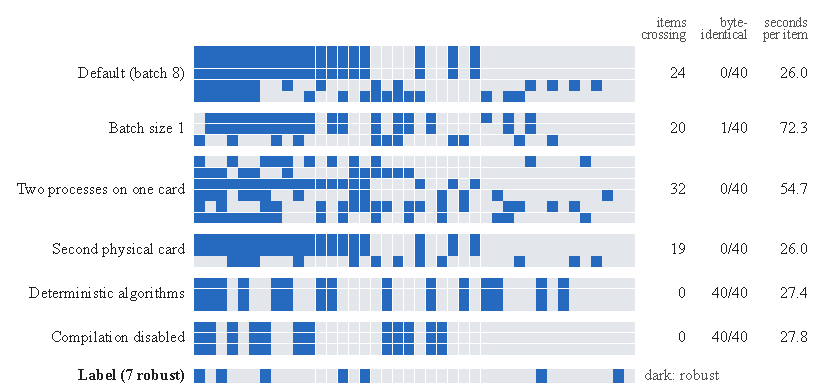
\includegraphics[width=\linewidth]{fig_rumore.pdf}
\caption{Predictions of the official pipeline for 40 preliminary public problems (columns) in 23 executions on DeepSeek (rows), by configuration; the last row is the label, dark cells are robust, and columns are sorted by how often they are predicted robust. At right: items whose prediction changes across the configuration's runs (more runs, more crossings), items whose generated text is byte-identical in all of them, and seconds per item.}
\label{fig:noise}
\end{figure}

\begin{table}[t]
\caption{Repeatability of the official pipeline on DeepSeek, 40 public problems, by configuration, in the order of Figure~\ref{fig:noise}. ``Crossings'': items whose prediction changes across the configuration's runs. ``Identical'': items whose generated text is byte-identical in all runs. Cost is runtime against the default configuration. Card 0 and card 1 are the two GPUs of the same machine. With two processes on one card, any five of its six runs give 29 to 31 crossings.}
\label{tab:reexec}
\centering
\small
\begin{tabular}{@{}lllllll@{}}
\toprule
\textbf{Configuration} & \textbf{Card} & \textbf{Runs} & \textbf{Crossings} & \textbf{Identical} & \textbf{Correct per run} & \textbf{Cost} \\
\midrule
Default (batch 8) & 0 & 5 & 24/40 & 0/40 & 24, 24, 24, 23, 24 & reference \\
Batch size 1 & 0 & 3 & 20/40 & 1/40 & 20, 21, 24 & +178\% \\
Two processes on one card & 0 & 6 & 32/40 & 0/40 & 24 to 28 & +110\% \\
Second physical card & 1 & 3 & 19/40 & 0/40 & 24, 24, 21 & +0\% \\
Deterministic algorithms & 0 & 3 & 0/40 & 40/40 & 24, 24, 24 & +5\% \\
Compilation disabled & 1 & 3 & 0/40 & 40/40 & 25, 25, 25 & +7\% \\
\bottomrule
\end{tabular}
\end{table}

\paragraph{Two candidate remedies.} Deterministic algorithms (PyTorch's, in warn-only mode, with deterministic cuDNN and a fixed cuBLAS workspace; Appendix~\ref{app:C}) and disabled compilation each made the generated text byte-identical in three sequential runs, at 5 to 7\% runtime cost. On card 0, the default configuration produced 24 crossings in five runs. Each remedy ran on one card where the default had produced crossings, each run in a new process, with no other process on that card. Three identical runs are weak evidence: the default configuration also gave three identical runs on card 0 before its fourth diverged, and five of its eight runs on the two cards shared one output. The two remedies produced different outputs, predicting 15 and 12 of the 40 problems robust, and because they ran on different cards we cannot tell whether the difference comes from the configuration or from the card. Neither gained more than one item (24 and 25 correct).

\paragraph{Distinct outputs.} The 23 executions fall into 14 distinct outputs, byte-identical within each. The same output appeared on both cards, and two runs launched in the same second on one card produced different outputs, so the output is not a property of the card alone; what selects it is not established. As only 7 of the 40 problems are robust and crossings largely cancel, accuracy moved much less than predictions: 21 to 24 correct in the default configuration on either card and 24 to 28 with two processes on one card, always below the 33 of the majority constant. An exploratory repetition of the official score extraction, whose third run ranks the 164 labeled problems at Spearman 0.24 against the first two, is in Appendix~\ref{app:C}.

\section{Regenerating the labels with our own protocol}\label{sec:labels}

\paragraph{Our labeling protocol.} We identified the organizers' perturbation families in the preliminary data (rephrase, rename, domain, distract, typos), regenerated them with gpt-oss-120b prompted with public examples, and gated each variant with gpt-oss-120b. An answer counts as correct when it matches gpt-oss-120b's answer on the original problem, because the preliminary data carry no answers; we did not check this key against the answers of the collections the problems come from. On the organizers' machine, with vLLM 0.28.0 [8] outside the official image, we labeled four models with two independent draws of variants (A and B, about 40 accepted variants per problem): 10 samples on the base problem and one per variant, at temperature 0.6, top-p 0.95 and at most 16,384 new tokens. Draw A's variants were also re-sampled with a new seed (A$'$). A label is robust when at least 6 of the 10 base samples are correct and every variant is answered correctly; unlike the earlier rule's conjunction, this requires the base problem to be solved.

A chain that reaches our cap is scored by the last boxed answer it contains, and counts as wrong without one; the organizers also count a response that reaches their limit without a parseable final answer as wrong [4]. Our protocol differs from the organizers' in perturbations, answer key, rule and sampling (one answer per variant, against 10 in the files behind most of their DeepSeek labels). Its decoding differs from the settings they publish, and its prompt may differ from the one behind their labels, which they have not stated.

\begin{table}[t]
\caption{Agreement of labels regenerated with our protocol: Cohen's kappa. The three columns for A and B treat variant chains that reached the 16,384-token cap in three ways: scored as in the protocol (by their last boxed answer, if any), dropped, or all counted as correct. The first of these columns and the A and A$'$ column give 95\% percentile bootstrap intervals over problems, and the script of Appendix~\ref{app:E} gives them for the other two. A problem has a label in a draw when it has at least one accepted variant (160 in A, 159 in B). Kappa between A and B uses the 159 problems labeled in both (150 for Qwen3.5-4B and 156 for DeepSeek when truncated chains are dropped), and between A and A$'$ 160. ``At cap'': percentage of variant chains that reached the cap in draws A and B. ``Robust'': percentage of problems labeled robust in draw A, as scored. The last column gives kappa of draw A with the organizers' preliminary DeepSeek labels: on the 138 published ones, and on the 160 that include 22 labels we derived (Section~\ref{sec:data}).}
\label{tab:label}
\centering
\small
\setlength{\tabcolsep}{3pt}
\begin{tabular}{@{}llllllll@{}}
\toprule
& & & \multicolumn{3}{l}{\textbf{A and B, truncated variant chains}} & & \\
\cmidrule(lr){4-6}
\textbf{Model} & \textbf{At cap} & \textbf{Robust} & \textbf{as scored} & \textbf{dropped} & \textbf{correct} & \textbf{A and A$'$} & \textbf{Organizers'} \\
\midrule
Skywork & 1.2, 1.5 & 74 & 0.44 [0.28, 0.59] & 0.39 & 0.39 & 0.79 [0.67, 0.89] & none \\
DeepSeek & 5.1, 6.1 & 39 & 0.41 [0.26, 0.55] & 0.35 & 0.36 & 0.46 [0.33, 0.59]$^{*}$ & 0.011; 0.025 \\
Olmo & 1.1, 0.9 & 68 & 0.38 [0.21, 0.54] & 0.39 & 0.39 & 0.65 [0.52, 0.78] & none \\
Qwen3.5-4B & 22.1, 29.2 & 9 & 0.18 [$-$0.06, 0.39] & 0.26 & 0.44 & not run & none \\
\bottomrule
\end{tabular}
\par\smallskip{\footnotesize $^{*}$On DeepSeek, A$'$ also received the answer-format line (end of this section), so this entry mixes seed and prompt.}
\end{table}

\paragraph{Results.} Under our protocol, two independent draws of variants give labels that agree at kappa 0.35 to 0.44 on Skywork, Olmo and DeepSeek, whether truncated variant chains are scored as in the protocol, dropped or all counted as correct (Table~\ref{tab:label}). On Qwen3.5-4B, 22 to 29\% of the variant chains reach the cap. Scoring these chains as in the protocol, dropping them or counting them all as correct gives agreement of 0.18, 0.26 and 0.44, and a robust share in draw A of 9\%, 83\% and 79\%. On Skywork, re-sampling the same variants with a new seed agrees far more than drawing new variants (0.79 against 0.44), so its label depends more on the variants than on the seed; on Olmo the gap is smaller (0.65 against 0.38), and on DeepSeek, where A$'$ also changed the prompt, it is 0.46 against 0.41.

Draw A's DeepSeek labels agree with the 138 labels the organizers published at kappa 0.011 [$-$0.13, 0.17], and with the 160 that include 22 of our derived labels at 0.025 [$-$0.12, 0.18]. Of the 36 problems with a published robust label, draw A calls 20 non-robust, and 4 of these change when truncated variants all count as correct. Of the 102 with a published non-robust label, draw A calls 44 robust. The reliability of the organizers' labels remains unmeasured. A retrospective calculation on the same saved answers with the main-phase threshold rule, applied as its pre-registration fixed it, with no filter on the base problem (Appendix~\ref{app:C}), gives test-retest point estimates between 0.34 and 0.56, below the pre-registered bar of 0.60, though three of the four intervals include it.

\paragraph{The prompt changes our labels.} In a first run with the bare problem text, later discarded, \mbox{Qwen3.5-4B} gave a final answer in the expected format in only 5 of its 1,640 base samples in draw A. With one instruction line requesting the format, 145 of 164 problems passed the base condition, against none. DeepSeek passed it on 147 of 164 with or without that line; its draws A and B ran without the line and A$'$ with it, and on the same variants its robust share moved from 39\% to 51\% of the 160 labeled problems, a change that mixes prompt and seed. Under our protocol, the label of Qwen3.5-4B therefore depends on the prompt. Whether this affects the organizers' labels is unknown: their baselines repository has a solve prompt that asks for an ANSWER line, but they have not said whether it was used for labeling (R3).

\section{The falsification campaign}\label{sec:campaign}

Table~\ref{tab:campaign} summarizes the campaign; Appendix~\ref{app:A} lists all 31 entries and explains three traps (rule T, the oracle H13, the duplicated pairs behind H2) and two pitfalls of the data. All entries use the preliminary data, except H16 to H18, which were scored on the 17 items of the warmup evaluation task.

\begin{table}[t]
\caption{The campaign in brief, in 19 of its 31 entries (Appendix~\ref{app:A} lists all). Ground truth is DeepSeek's and the preliminary pairs' unless stated; accuracy differences are in points against each pre-registration's baseline. H1, H7 and T count the 52 duplicated DeepSeek pairs twice; counted once, no verdict changes.}
\label{tab:campaign}
\centering
\small
\begin{tabular}{@{}L{5.5cm}L{1.9cm}L{5.6cm}@{}}
\toprule
\textbf{What we tested} & \textbf{Entries} & \textbf{Outcome} \\
\midrule
Text features; robustness as a property of the problem; labels, base accuracy and difficulty order across models & H1 to H5, H7 & rejected; H2 gained only when the duplicated pairs were counted twice \\
Official uncertainty features, logistic regression & H10 & 0.774 against a majority constant of 0.756, within the 0.692 $\pm$ 0.101 of the proposal [1] (method substituted) \\
Features cached for other models; per-target thresholds & H12, H13 & H12 rejected; the H13 ceiling withdrawn, $-$2.8 points when forced to rank \\
Our perturbation families, translation, self-consistency, the organizers' families regenerated (pilot), representation shift & H19, H22, H30 to H33 & rejected: kappa at most 0.02, AUROC at most 0.615 \\
Probes on DeepSeek's hidden states: ours and the organizers' published artifact & H36, H35 & survive their nulls; ours adds no detectable gain over length, and the artifact's score is probably in-sample \\
Trivial-robust rule, post hoc & T & a trap: +6.0 points on the preliminary pairs, +0.0 on \texttt{val-sample} \\
Identical bundles re-executed (warmup, 17 items) & H18 & noise confirmed: 11, 9, 11 and 11 correct \\
\bottomrule
\end{tabular}
\end{table}

\paragraph{Length and probes.} The character count of the problem alone orders the 164 DeepSeek labels at AUROC 0.704. Our logistic probe on DeepSeek's last-token hidden states, with layer and regularization chosen by inner cross-validation, reaches 0.710 out of fold with the original fold assignment. Over 20 other assignments, passed through the second-stage model below, it gives 0.57 to 0.76 (mean 0.69). Its scores correlate with length at Spearman +0.55, and residualized on log character count it gives 0.62. Its permutation null, rerun with 1{,}000 permutations of the whole nested procedure (the first version used 60, where 500 were pre-registered), gives $p = 0.002$. Restricted to the 138 published labels, these out-of-fold scores give 0.714 and length 0.733; retrained on those 138 alone with H36's procedure and seed, the probe gives 0.620. Combined with length in a second-stage model fitted on common outer folds, the probe changes AUROC over length alone by +0.005 on the 164 labels and by $-$0.010 on the 138 published ones (median bounds of the per-assignment 95\% intervals: $-$0.03 to 0.04, and $-$0.04 to 0.02): we detect no gain from adding the probe to length (Appendix~\ref{app:C}). This analysis replaces an earlier combination that leaked labels (Appendix~\ref{app:D}).

The organizers' published DeepSeek probe artifact orders the 164 DeepSeek labels at 0.739 with the aggregation we pre-registered and at 0.709 with its own, and at 0.62 and 0.57 residualized on log character count; its controls trained on shuffled labels give 0.68 at layer 31. The artifact does not record its training data; we infer that 137 of the 164 problems were among the public rows it was trained on, so these scores are probably largely in-sample. These length controls, which play the role of control tasks [7], were post hoc. Whether either probe reads anything beyond length that bears on robustness is not established. Apart from the three traps of Appendix~\ref{app:A}, no signal we scored by accuracy beats the majority constant by more than about one standard error on the preliminary labels, most of them DeepSeek's.

\section{Our entries}\label{sec:entries}

Our entry V8, pre-registered on 13 September, is the whole rule \texttt{return~[len(p)~>=~98 for~p~in~problems]}, with the threshold at the lower median of the 174 preliminary problems and the direction fixed on the preliminary pairs. On the original main-phase tasks it scored 11/21 and 10/19, like our entry v6 and the organizers' own entries. None of these beat the majority constant, which scores at least 11/21 and 10/19 on these tasks, and on so few items the ties do not show that length carries no signal (95\% Wilson intervals 0.32 to 0.72 and 0.32 to 0.73). On the 71 labeled rows of the official training set (revision of 17 September; 36 distinct problems), V8 differs from the all-robust constant on only 6 rows and is wrong on all 6 (46/71 against 52/71): too few to say what length is worth on official data. On the replacement tasks of 16 September, before and after the evaluation changed on 15 October [6], it predicted robust for every item (10/21 and 7/14), like an all-robust control. For the final test we nominated V8 (Codabench 1016713) and the constant (1016732), both on the Main track; our pre-registered predictions will be scored there (Appendix~\ref{app:B}).

\section{Recommendations}\label{sec:recs}

These rest mostly on DeepSeek and the preliminary data, and should be checked on the other models.
\begin{itemize}
\item \textbf{R1. Remove the variation between runs, and test the remedy:} on the same card with independent restarts, under load and across cards.
\item \textbf{R2. Repeat only where it decides something:} at the warmup's re-execution noise (a standard deviation of 1.0 item on 17, itself estimated from four runs), a one-item gap needs about eight runs per entry to reach two standard errors, so repeat only entries that run a model and sit near a prize boundary.
\item \textbf{R3. Say which prompt and decoding settings produced each released label file,} at least after the close.
\item \textbf{R4. Measure the label's reliability directly,} with two independent draws of variants labeled by the official process.
\item \textbf{R5. Show floors and noise on the leaderboard:} a row per constant predictor, the re-execution noise and binomial intervals.
\item \textbf{R6. Require a length control in white-box ablations.}
\item \textbf{R7. Remove the leaking field} \texttt{permutation\_type} from the aggregated datasets (Appendix~\ref{app:A}).
\end{itemize}

\paragraph{Code and data.} Our code, bundles, pre-registrations and outcome files are released at \href{https://github.com/Dan23RR/aimo-instrument}{\nolinkurl{github.com/Dan23RR/aimo-instrument}}. Its folder \texttt{reproduce/} recomputes the main tables from saved outputs and the six preliminary datasets, and the other numbers come from the dated records in \texttt{archive/} (Appendix~\ref{app:E}).

%%%%%% End of the main text: the six pages end here; the Limitations do not count %%%%%%
\label{fine-testo}

\section*{Limitations}

\begin{enumerate}[leftmargin=1.6em, itemsep=2pt, topsep=4pt, parsep=0pt]
\item \textbf{Preliminary data, not official data.} We did not repeat our label and probe analyses on the official training set, beyond the evaluation of V8 and a five-row check of our labels (Appendix~\ref{app:C}). Findings on label reliability and predictability may not generalize to the official evaluation setting.
\item \textbf{Our protocol, not the official one.} We did not regenerate labels with the organizers' published settings (100,000 tokens, temperature 1.0), with 10 answers per variant as in the files behind most DeepSeek labels, or on \texttt{train-main-v2}. The three treatments of truncated variant chains show how much our cap moves agreement between our draws; all three score base samples that reach the cap as the protocol does, and none of them reproduces longer decoding or a different temperature. Our low agreement with the organizers' labels is a fact about our process.
\item \textbf{One model.} We ran the probes, the re-execution study of Section~\ref{sec:reexec} and the comparisons of our regenerated labels with the organizers' preliminary labels only on DeepSeek.
\item \textbf{Re-execution.} We did not run the two candidate remedies on the same card, so card and configuration are confounded; we did not test either remedy under contention or on both cards, and we used 40 problems and one image.
\item \textbf{Records.} Some analyses rest on re-created scripts or dated records (Appendix~\ref{app:D}). Nothing here estimates performance on the final held-out problems.
\end{enumerate}

\section*{AI usage statement}

In this work, we used one generative AI tool, Claude (Anthropic), through Claude Code, for ideation, coding, analysis and writing. Ideation: it drafted the pre-registrations, including hypotheses, predictions and kill criteria, and searched and summarized the literature and the public records, including the organizers' Discord channels and the author's correspondence with them. Coding: it wrote the solution code of our bundles and the analysis and extraction scripts, ran them, and operated the organizers' virtual machine over SSH. Analysis: it computed and interpreted the results and ran automated adversarial reviews of hypotheses, drafts and code. Writing: it drafted the correspondence, this report and its revision after review.

It also made most of our Codabench uploads through the author's browser at the author's instruction. There were two exceptions: one resubmission (925822, 14 September), made without a specific instruction, and one submission that the author had not approved, sent in error and rejected before import (1016734, 28 October).

Language models were also components of our method: gpt-oss-120b generated and gated the perturbation variants and supplied the reference answers of Section~\ref{sec:labels}, and phi-4 translated problems for H22. The final decisions on the direction of the work, on the submissions (with the two exceptions above), on the nominations for the final test and on the claims of this report were the author's, and the author sent all correspondence personally. The author has reviewed all AI-assisted work and takes full responsibility for the final content of this report.

\begin{ack}
We thank Michal Štefánik, Róbert Belanec and the AIMO Interpretability team for the compute grant, a virtual machine with two GPUs, and for answering our questions; on 2 November they confirmed that the measurements taken on their machine may appear in this report. We also thank the three reviewers and the program chairs: two reviewers checked our analyses against the released code and data, and their checks corrected several of our claims. Other GPU time was rented on Modal and paid by the author or covered by Modal's platform credit. This work received no other funding, and the author has no competing interests.
\end{ack}

\section*{References}
{\small
[1] M. Štefánik, P. Mondorf, A. Waldis, Q. Liu, C. Yang, M. Spiegel, J. Kuchař, M. Kadlčík, A. Vawda-Oomerjee, C. Liu, S. Frieder, B. Plank, F. Barez and P. Stenetorp. AIMO Interpretability Challenge. CoRR, abs/2607.13899, 2026. doi:10.48550/arXiv.2607.13899.

[2] H. He and Thinking Machines Lab. Defeating Nondeterminism in LLM Inference. Thinking Machines Lab: Connectionism, 2025.

[3] J. Yuan, H. Li, X. Ding, W. Xie, Y.-J. Li, W. Zhao, K. Wan, J. Shi, X. Hu and Z. Liu. Understanding and Mitigating Numerical Sources of Nondeterminism in LLM Inference. NeurIPS 2025. arXiv:2506.09501.

[4] AIMO Interpretability Challenge website and FAQ. \url{https://aimo-interp.github.io} (accessed 28 October 2026), and its source repository aimo-interp/aimo-interp.github.io on GitHub.

[5] aimo-interp/getting-started and aimo-interp/baselines, GitHub repositories: README and issues \#6 and \#10 of getting-started; aimo-interp datasets on Hugging Face, including \texttt{train-main-v2} and \texttt{val-sample}.

[6] AIMO Interpretability Challenge Discord, \#announcements and \#qa: 5, 15 and 22 September, 9, 15, 16 and 20 October 2026.

[7] J. Hewitt and P. Liang. Designing and Interpreting Probes with Control Tasks. EMNLP-IJCNLP 2019.

[8] W. Kwon et al. Efficient Memory Management for Large Language Model Serving with PagedAttention. SOSP 2023.

[9] D. Hendrycks et al. Measuring Mathematical Problem Solving With the MATH Dataset. NeurIPS 2021 Datasets and Benchmarks Track. arXiv:2103.03874.
}

%%%%%% End of the references %%%%%%
\clearpage
\appendix
\raggedright

\section{The hypotheses, three traps and two pitfalls of the preliminary data}\label{app:A}

Section~\ref{sec:campaign} summarizes these entries. Unless stated, the ground truth is the 335 public pairs for H1 to H9 and T, the other models' preliminary labels for H12 to H15, the 17 items of the warmup evaluation set for H16 to H18, and DeepSeek's labels for the others. Validation that fits on some problems and tests on others is grouped by problem. The cross-model tests H7 and H12 to H15 hold out the model but not the problem, so part of them is in-sample; H7, H12, H14 and H15 were rejected anyway, and H13 is withdrawn. Numbers are accuracy points against each pre-registration's baseline unless they are kappa or AUROC.

{\small\setlength{\tabcolsep}{4pt}\renewcommand{\arraystretch}{1.2}
\begin{longtable}{L{1.1cm}L{3.9cm}L{5.6cm}L{2.0cm}}
\toprule
\textbf{ID} & \textbf{Hypothesis} & \textbf{Result} & \textbf{Verdict} \\
\midrule
\endfirsthead
\toprule
\textbf{ID} & \textbf{Hypothesis} & \textbf{Result} & \textbf{Verdict} \\
\midrule
\endhead
\bottomrule
\endlastfoot
H1 & The problem text predicts robustness (32 features) & 0.675 against 0.761, $-$8.7 ($-$7.4 with the duplicated pairs counted once) & rejected \\
H2 & Robustness is a property of the problem & with the 52 duplicated pairs counted once, z~=~0.88 and $-$1.3 against the per-model majority (bar 4.0); z~=~4.04 and +3.4 only when they are counted twice & rejected \\
H3 & One model's label predicts another's & $-$7.3 & rejected \\
H4 & One model's base accuracy predicts another's robustness & $-$11.8 & rejected \\
H5 & The difficulty order transfers across models & $-$25.4 & rejected \\
H6 & The same, with the oracle number of positives & $-$13.0 & ceiling (no kill criterion) \\
H7 & Base accuracy beats the prior on held-out models & $-$1.2 against the per-model majority that its pre-registration named (+0.0 against the global prior we used instead) & rejected \\
T & Robust if and only if base accuracy is below 0.05 (post hoc; see the traps below) & +6.0 on the 335 public pairs, +0.0 on \texttt{val-sample} & trap (no kill criterion) \\
H10 & The official uncertainty features reach the accuracy the proposal reports & 0.774 against a majority constant of 0.756, within 0.692 $\pm$ 0.101 [1]; a logistic regression on 13 of the 14 features of our own A100 re-implementation of the extraction (three of them constant), substituted for the official regressor & confirmed (method substituted, not declared at the time) \\
H11b & Length, saturation and trend features add signal & $-$1.8 and $-$2.5 & rejected \\
H12 & A cached model's uncertainty features predict other models & $-$16.5 & rejected \\
H13 & The same, with a threshold chosen per target & +7.3, from thresholds chosen on the scored items; $-$2.8 when forced to rank & withdrawn (no kill criterion) \\
H14, H15 & Calibration by the target's rate or by the global rate & $-$2.8 and $-$10.1 & rejected \\
H16 & Every model measured by itself beats the constant & 10/17 against 9/17 on one execution, inside the noise of H18 & survives, within noise \\
H17 & A gpt-oss threshold calibrated on \texttt{val-sample} beats H16 & 11/17, then 9, 11 and 11 on re-execution; 9/17 meets the kill criterion & not established \\
H18 & Identical bundles score differently across executions & 11, 9, 11 and 11 correct & confirmed (no kill criterion) \\
H19 & Our five mechanical perturbation families reproduce the organizers' preliminary label & accuracy 0.354 against 0.788, kappa 0.02 & rejected \\
H20 & A threshold tuned on our label transfers & 0.212 against 0.788 & rejected \\
H22 & Stability under translation reproduces the organizers' preliminary label & 0.507 against 0.740, kappa $-$0.10 & rejected \\
H23 & A threshold tuned on it transfers & +0.0 & rejected \\
H29 & Representation-distance features are repeatable (gate; written plan, not a frozen pre-registration) & ICC 0.997 to 0.999, from the dated outcome file & passes \\
H30 & The representation shift under perturbation predicts the label (written plan) & AUROC 0.615, below the kill threshold of 0.655; character count 0.704 (0.705 in E11's own computation) & rejected \\
H31 & The direction of that shift predicts the label (written plan) & AUROC 0.555 & rejected \\
H32 & The organizers' families, regenerated (pilot), reproduce their label & kappa $-$0.001 on four families, $-$0.030 with all five & rejected \\
H33 & Self-consistency over 8 samples predicts the label & AUROC 0.502 & rejected \\
H35 & The organizers' published probe artifact orders the 164 DeepSeek labels & 0.739 under the pre-registered aggregation and 0.709 under its own; 0.62 and 0.57 once residualized on log character count; its shuffled-label controls give 0.68 at layer 31 & survives its null; probably in-sample, not separated from length \\
H36 & Our linear probe, nested cross-validation, orders the 164 DeepSeek labels & 0.710 out of fold, above its permutation null, and 0.62 once residualized on log character count; 0.714 against 0.733 for length on the 138 published labels (Appendix~\ref{app:C}) & survives its null; no detectable gain over length \\
E13b-1 & Under the main-phase rule our regenerated label is test-retest reliable (kappa at least 0.60 on 3 of 4 models) & 0.34 to 0.56, retrospective (Appendix~\ref{app:C}) & rejected \\
E13b-2 & Under the main-phase rule it agrees with DeepSeek labels we computed with that rule from the preliminary data (kappa at least 0.40) & 0.02 [$-$0.09, 0.13] & rejected \\
E13b-3 & The labeling rule drives the instability of our regenerated labels & a gain of at least 0.15 on 2 of 4 models, where 3 were required; 0 of 4 on common problems & rejected \\
\end{longtable}
}

Not in the table are H8, H9, H21, H24 and H25 to H28. H8 is an oracle ceiling: 0.774, +1.8 points against the global constant and +0.4 against the per-model majority, with the duplicated pairs counted once. The outcome of H9 became rule T. H21 and H24 needed H19 and H20, and H22 and H23, to survive, so they were not run. H25 to H28 are entries of the E11 plan that its outcome file does not report under these identifiers. H25 is an anomaly of our own re-implementation of the extraction, found before the plan. H26 is the list field of the first pitfall below. H27 is a label-noise ceiling, which the plan itself closed with a resampling estimate instead of a test. H28 is the text-only baseline, which became character count (Appendix~\ref{app:D}). Three further E11 tests were not run (Appendix~\ref{app:D}). V4, an entry submitted once against its own pre-registered rule, is in Appendix~\ref{app:D}.

\paragraph{Three traps.} Rule T gains six points on the public pairs and nothing on \texttt{val-sample}, because the trivially robust items (base accuracy 0, robust under the conjunction) are absent there. The oracle H13 chose each target's threshold among all cut points on the very items it was scored on; forced to rank the items and to predict the true number of positives, it gave $-$2.8. H2 owed its survival to one measurement published under two model names and counted twice; counted once, its z falls from 4.04 to 0.88.

\paragraph{Two pitfalls of the preliminary data.} In the three aggregated datasets, the field \texttt{permutation\_type} is a list if and only if the item is robust, because the aggregation merges all perturbation types into one row for robust items and keeps one row per retained type otherwise, usually a single type. The rule ``robust if the field is a list'' reproduces all 223 labeled rows of the three datasets, and the field does not exist at inference (recommendation R7). And 20 of the 80 robust pairs among the 335 have base accuracy 0. None of them carries a published label, so they are robust only under the conjunction we used to derive their labels, while \texttt{val-sample} has no labeled pair with base accuracy below 0.05.

\section{Pre-registered predictions for the final evaluation}\label{app:B}

P1 was written on 7 September 2026, P-V8 on 13 September and P-V8b on 21 September. They are translated from the dated files and shortened. We omit the runtime predictions (under 60 seconds), which we could not score because the bundles log no runtime. A second prediction written with P1 on 7 September concerns another participant's final score and is not reported here.

\begin{itemize}
\item \textbf{P1.} The top-ranked entry's accuracy on the final held-out problems will lie within two binomial standard errors of that set's majority-class constant.
\item \textbf{P-V8.} If the organizers had neutralized length, V8 would score between 0.45 and 0.55 on both tracks (stated beforehand as the most likely outcome); if they had not, and the set was balanced, about 0.66. Observed on the original tasks: 0.52 and 0.53, inside the first band; on 21 and 19 items, however, 0.66 lies inside the 95\% intervals of both scores, so the scores do not exclude the second.
\item \textbf{P-V8b}, on the replacement tasks: the same bundles work with the new ingestion and score 6 to 15 of 21 and 4 to 10 of 14. Observed: coverage 1.0, no invalid predictions, 10/21 and 7/14, inside the bands but degenerately, since the rule predicted robust for every item.
\end{itemize}

\section{Protocols, run manifest and recalculations}\label{app:C}

\paragraph{Hardware and software.} The generation runs used the organizers' virtual machine with two NVIDIA RTX PRO 6000 Blackwell Server Edition GPUs (96 GB each), the evaluation workers' model, from 8 September 2026. Each run used one GPU; the Olmo-3-7B-Think A$'$ labels combine two runs, one on each card (below).
\begin{itemize}
\item \textbf{Official runtime image.} Section~\ref{sec:reexec} and the official score channel (E16) ran inside it: {\footnotesize\path{ghcr.io/aimo-interp/aimo-codabench-runtime:torch2.12.1-cuda13.2-cudnn9-transformers5.13.0-sklearn1.8.0-kernels0.15.2}}, digest {\footnotesize\path{sha256:fb4dab6343de7ce022ddd7906493f9ced16ff9008d497326a781d1e5adc8207a}}. They used the official extraction and regressor as shipped in our bundles: greedy decoding, at most 4,096 new tokens, static cache, batch 8.
\item \textbf{Labeling environment.} Section~\ref{sec:labels} ran with vLLM 0.28.0, torch 2.13.0 and transformers 5.16.1 (driver 610.57.04 with CUDA 13.3 on the machine, CUDA 13.0 runtime libraries in the environment) in a separate environment on the same machine; \texttt{vm\_backup/AMBIENTE\_VM\_2026-09-17.txt} lists every package.
\item \textbf{Model revisions.} Hugging Face snapshot hashes: Qwen3.5-4B \texttt{851bf6e8}, Skywork-OR1-Math-7B \texttt{fcef970f}, Olmo-3-7B-Think \texttt{d97e442d}, DeepSeek-R1-0528-Qwen3-8B \texttt{6e8885a6}, gpt-oss-120b \texttt{b5c939de}. The full hashes are in the run logs.
\item \textbf{Analyses.} They ran on CPU: E13's analysis and E15's evaluation, up to 14 September, on the virtual machine (Python 3.12, NumPy 2.3.5, scikit-learn 1.9.1), the others on the author's computer (Python 3.11.12, NumPy 2.4.4 and scikit-learn 1.8.0, as recorded for the runs of September and November). The release pins every output by SHA-256 in \texttt{MANIFEST.tsv}.
\end{itemize}

\needspace{8\baselineskip}
\paragraph{Run manifest.}
\begin{itemize}
\item \textbf{Where they ran.} The scripts in \texttt{vm/} written up to 14 September (setup, generation, extraction, E13's analysis and E15's evaluation), after which the machine stayed idle, and the clean-up script of 17 September ran on the virtual machine; the later ones ran on the author's computer.
\item \textbf{Outputs} are in \texttt{vm\_risultati/} unless the table gives another path.
\item \textbf{GPU-hours} are times from the logs (\texttt{reproduce/compute\_hours.py}). They include model loading except for the E13 labels, a difference under 1\%.
\end{itemize}

{\small\setlength{\tabcolsep}{4pt}
\begin{longtable}{L{2.4cm}L{3.2cm}L{2.2cm}>{\raggedright\arraybackslash\footnotesize}p{4.8cm}}
\toprule
\textbf{Run} & \textbf{Where it ran} & \textbf{GPU-hours} & \textbf{Outputs} \\
\midrule
\endfirsthead
\toprule
\textbf{Run} & \textbf{Where it ran} & \textbf{GPU-hours} & \textbf{Outputs} \\
\midrule
\endhead
\bottomrule
\endlastfoot
E13 variants & virtual machine & 1.15 and 1.20 & \path{e13/varianti_D1.parquet}, \path{e13/varianti_D2.parquet} \\
E13 labels & virtual machine, one queue per card & 64.4, in the logs of the 11 runs of Table~\ref{tab:label} & \path{e13/etich_*.parquet} \\
E13b, main-phase rule & author's computer & CPU only & \path{e13b_regola_nuova_2026-09-21.txt} \\
E14 re-execution & virtual machine, official image & 8.4 & \path{e14/out/*.jsonl}, \path{e14/log/} \\
E15 extraction & virtual machine & under 0.1 & \path{vm_backup/estratto/work/aimo/e15/hs_*.npz} \\
E15 probes & the virtual machine's CPU on 14 September, then the author's computer & CPU only & \path{e15_*}, \path{e15r/}, \path{vm_backup/estratto/work/aimo/e15_valuta.log} \\
E16 score channel & virtual machine, official image & 5.9 & \path{e16_*.jsonl}, \path{e16nodet/} \\
\end{longtable}
}

\paragraph{Commands.} Script paths are relative to \texttt{archive/}, the working folder of the repository. The scripts in \texttt{vm/} that ran on the virtual machine use paths under \texttt{/work/aimo}. \texttt{M} stands for the model, and in E14 \texttt{C}, \texttt{r}, \texttt{g} and \texttt{t} for the configuration, repetition, card and process tag.
\begin{itemize}
\item \textbf{E13 variants.} \texttt{vm/e13\_varianti.py -{}-draw~D1 -{}-seed~20260913 -{}-n~164 -{}-k~10}, and \texttt{-{}-draw~D2 -{}-seed~20260914}. The model gpt-oss-120b generates, solves and gates the variants (prompts below).
\item \textbf{E13 labels.} DeepSeek A and B ran an earlier version of \texttt{e13\_etichetta.py} that sent the bare problem text (now \texttt{-{}-prompt~nudo}); every other run behind Table~\ref{tab:label}, DeepSeek A$'$ included, used the explicit prompt. Draw A: \texttt{vm/e13\_etichetta.py -{}-model~M -{}-cond~A -{}-draw~D1 -{}-seed~20260921 -{}-prompt~esplicito}; B: \texttt{-{}-cond~B -{}-draw~D2 -{}-seed~20260922}; A$'$: \texttt{-{}-cond~Ap -{}-draw~D1 -{}-seed~20260923}. \texttt{vm/e13\_coda.sh} launched one queue per card (its logs are in \path{vm_backup/estratto/work/aimo/}); the card 0 queue ran an earlier version that passed no \texttt{-{}-prompt} flag, so DeepSeek A$'$ got the default of \texttt{e13\_etichetta.py}, the explicit prompt.
\item \textbf{E13b.} \texttt{vm/e13b\_regola\_nuova.py}, on the saved E13 answers; retrospective (below).
\item \textbf{E14.} \texttt{vm/e14\_all.sh 40 "C0 C1 C2 C3"} and \texttt{vm/e14\_extra.sh 1 "C5 C4"}. Each run is \texttt{e14\_run.py -{}-cond~C -{}-rep~r -{}-gpu~g -{}-tag~t -{}-n~40} inside the official image: 23 runs on DeepSeek. In the 8.4 GPU-hours the two processes of each contention pair, which shared one GPU, count once (20 runs).
\item \textbf{E15 extraction.} \texttt{vm/e15\_estrai.py -{}-model~deepseek-ai/DeepSeek-R1-0528-Qwen3-8B}, with and without the official system prompt: one forward pass per problem, last input token, all 37 hidden-state indices, at most 2,048 tokens.
\item \textbf{E15 probes.} \texttt{vm/e15\_valuta.py} ran H35, H36 and the first null (60 permutations) on 14 September, on the virtual machine's CPU; its log is \path{vm_backup/estratto/work/aimo/e15_valuta.log}. The file \path{vm_risultati/e15_valuta_2026-09-14.txt} is a later run of that day, by the file times in \path{vm_backup/MANIFEST_backup_aimo_2026-09-17.txt}, that stopped with an error at the null. H35's null is the 95th percentile, 0.602, of the AUROC of 20{,}000 random scores on the same labels, in either orientation. \texttt{vm/e15\_null\_nidificato.py} reran that null on 23 September with both grids of $C$, on the author's computer. E15-R (below) is \texttt{vm/e15r\_ricalcolo.py}, given an output folder and a number of worker processes (5 on the author's computer, 14.5 hours); its outputs are in \texttt{vm\_risultati/e15r}, and since it appends to existing files, a rerun needs a new folder. H35 needs the organizers' artifact \texttt{probe\_artifact.pkl} (hash below), which we do not redistribute.
\item \textbf{E16.} \texttt{vm/e16\_all.sh} and \texttt{vm/e16\_nodet.sh}, in the official image. Of the variables that \texttt{e16\_all.sh} sets, only the cuBLAS workspace variable reaches the extraction; \texttt{e16\_nodet.sh} sets neither.
\end{itemize}

The organizers' artifact used by H35 has SHA-256 {\footnotesize\texttt{8607478c7408922a6490adb7bda34d6a7d95403b7aa62f80dd3f2649139ccdeb}}. The listed logs total 82.8 GPU-hours. Not in the table:
\begin{itemize}
\item two complete runs of Qwen3.5-4B with the bare prompt (about 13 GPU-hours, no released log);
\item a partial run of Qwen3.5-4B A$'$ with the bare prompt (1.7 GPU-hours, included in the 82.8), discarded with them;
\item a run of Olmo-3-7B-Think A$'$ on card 1 (11.0 GPU-hours, 07:19 to 18:21 UTC on 10 September, from its queue log). Card 0 reached the same condition at 14:20, resumed from its partial file with 96 of the 164 problems done and finished the other 68, so the reported A$'$ labels come from both cards.
\end{itemize}
With these, the virtual machine ran about 107 GPU-hours, plus short smoke and feasibility tests. Our earlier runs on Modal used about 12 to 13 GPU-hours, mostly on A100 GPUs, as documented in their dated outcome files: the feature extraction behind H10, its pilot, and E9 to E12.

\paragraph{What can be recomputed.}
\begin{itemize}
\item \textbf{From saved outputs.} The scripts in \texttt{reproduce/} (Appendix~\ref{app:E}), which also read the six preliminary datasets; the other numbers come from the dated records in \texttt{archive/}.
\item \textbf{On a CPU, from the released hidden states.} Our probe (H36) and E15-R can be rerun end to end. H35 also needs the organizers' artifact.
\item \textbf{Only with the original GPUs and models.} The generation runs.
\end{itemize}

\paragraph{Re-execution configurations (Section~\ref{sec:reexec}).}
\begin{itemize}
\item \textbf{C0, default:} batch 8, on card 0, five runs.
\item \textbf{C1, batch size 1.}
\item \textbf{C2, deterministic algorithms:} \texttt{torch.use\_deterministic\_algorithms(True, warn\_only=True)}, \texttt{cudnn.deterministic = True}, \texttt{cudnn.benchmark = False} and \texttt{CUBLAS\_WORKSPACE\_CONFIG=:4096:8}.
\item \textbf{C3, contention:} two identical processes at the same time on card 0, three pairs.
\item \textbf{C4, second card:} the default on card 1.
\item \textbf{C5, compilation disabled:} \texttt{TORCH\_COMPILE\_DISABLE=1}, on card 1.
\end{itemize}
Runs within a configuration were sequential, each a new process. During these runs the other card was running another of our jobs. Two pre-registered predictions failed:
\begin{itemize}
\item batch size 1 did not make generation more repeatable: three runs gave three different outputs;
\item disabled compilation was predicted to land in one of the default outputs; it was byte-identical across its runs, but in an output of its own.
\end{itemize}
\texttt{reproduce/reexecution\_table.py} recomputes Table~\ref{tab:reexec} and the numbers of Figure~\ref{fig:noise}, and lists the 14 distinct outputs.

\paragraph{Variants and labels (Section~\ref{sec:labels}).}
\begin{itemize}
\item \textbf{Few-shot pool.} The generator saw five public examples of each family, drawn from a pool of 621 public examples (original, perturbed) over the five families. The texts are the organizers' and are not redistributed. \texttt{vm\_risultati/e13/fewshot\_pool\_ids.json} lists each example's problem identifier and SHA-256 hashes, and \texttt{reproduce/fewshot\_pool.py} rebuilds the pool from the downloaded preliminary datasets (verified on 23 November 2026: 621 of 621, byte-identical).
\item \textbf{Drawing the examples.} For draw seed $s$, problem $p$ and family $f$, the five examples are \texttt{random.Random("s|p|f").sample(pool[f] without p, 5)}.
\item \textbf{Generator.} gpt-oss-120b at low reasoning effort, temperature 1.0, top-p 1.0, at most 4,096 tokens, one request per problem and family, asking for 10 variants.
\item \textbf{Gate and reference answers.} gpt-oss-120b at medium effort, temperature 1.0, at most 8,192 tokens, solves the original and each variant. A variant is accepted if its text differs from the original, the length ratio lies between 0.7 and 4.0, and the solver's answer is unchanged. The solver's answer on the original is the reference answer.
\item \textbf{Labeling.}
  \begin{itemize}
  \item \textbf{Prompt.} Each model receives the instruction line (the second block below) followed by the problem, except DeepSeek in A and B, which received the bare text.
  \item \textbf{Sampling.} Temperature 0.6, top-p 0.95, at most 16,384 new tokens (raised from 8,192 before execution, after a test in which 2 of 3 problems saturated 8,192). There are 10 samples on the base problem and one per accepted variant.
  \item \textbf{Scoring.} A chain is scored by the last boxed answer it contains. Without one, including when it was cut at the cap, it counts as wrong.
  \end{itemize}
\end{itemize}

{\footnotesize
Generator prompt:
\begin{quote}\ttfamily
You create variants of mathematics competition problems for a robustness benchmark. Perturbation type: <family>. <family instruction> The variant must be a complete, self-contained problem with exactly the same final answer as the original. Do not solve the problem. Do not add hints or solutions. Here are 5 examples of this perturbation type: Example 1 Original: <public original> Variant: <public variant> (four more examples) Now write 10 different variants of the following problem. Make them genuinely different from each other. Output each variant between <variant> and </variant> tags, and nothing else. Original: <problem>
\end{quote}
Instruction line of the labeling prompt, also used by the solver of the gate:
\begin{quote}\ttfamily
Solve the following problem. Reason step by step, then give only the final answer inside \textbackslash{}boxed\{\}.
\end{quote}
}
The five family instructions, verbatim:
\begin{itemize}
\item rephrase: ``Rewrite the problem in different words while preserving exactly its mathematical content and its final answer.''
\item rename: ``Rename the variables, people, objects or entities in the problem while preserving its mathematical structure and its final answer.''
\item domain: ``Transfer the problem to a different real-world surface domain (a different story, setting and objects) while preserving exactly the same mathematical structure and the same final answer.''
\item distract: ``Insert irrelevant but plausible additional information (extra facts, numbers or context) that does not change the problem or its final answer.''
\item typos: ``Introduce harmless typographical or formatting noise (misspellings, spacing, punctuation, capitalisation) without changing the meaning of the problem or its final answer.''
\end{itemize}

\paragraph{The main-phase rule, retrospectively (E13b).} PREREG\_E13b was written on 21 September, before any calculation under the main-phase rule but after the E13 answers had been measured, so the calculation is retrospective.
\begin{itemize}
\item \textbf{The rule.} On the saved answers, a problem is robust if the largest drop in accuracy across families is at most 0.10 and non-robust if it is at least 0.25; problems in between get no label.
\item \textbf{No base filter.} As pre-registered, the primary calculation has no filter on the base problem, so a problem the model never solves counts as robust when no family lowers its accuracy.
\item \textbf{Test-retest, primary.} Kappa between A and B is 0.34 [0.13, 0.53] on 86 problems (Qwen3.5-4B), 0.49 [0.17, 0.76] on 132 (Skywork), 0.41 [0.09, 0.69] on 133 (Olmo) and 0.56 [0.36, 0.73] on 100 (DeepSeek). Because 58 to 95\% of the problems are labeled robust, kappa stays low even where raw agreement is high.
\item \textbf{Test-retest, secondary (S1).} On problems with at least 5 of 10 correct base samples in both draws, kappa is 0.31, 0.52, 0.40 and 0.55.
\item \textbf{Against the organizers.} Against DeepSeek labels that we computed with the same rule from the accuracy drops published in the preliminary data: 0.02 [$-$0.09, 0.13] on 133 problems.
\item \textbf{Against \texttt{train-main-v2}.} On its five labeled rows that fall on our problems and models, our labels agree with the official ones on 2 (draw A, one undefined) and 3 (draw B); five rows are too few to read.
\item \textbf{Truncated chains} are scored as in the protocol here too.
\end{itemize}

\paragraph{Subsampling (E13).} Subsampling DeepSeek's variants from 2 to 40 per problem leaves the mean kappa between A and B between 0.36 and 0.47, with no upward trend: more variants per problem do not make our labels more repeatable.

\paragraph{The official score channel (E16, exploratory).} We extracted the official regressor score on DeepSeek three times for the 174 public problems with the same code and image; this measurement was not pre-registered. The first run set the cuBLAS workspace variable and gave the same scores as the second, run without it, on all 174 problems. The second and third correlate at Spearman 0.24 over the 164 labeled problems. They give AUROC 0.487 and 0.602 in the regressor's own orientation; the paired bootstrap 95\% interval of their difference, $-$0.015 to 0.246, includes zero. The ranking of the problems was not reproduced in one of two repetitions; this does not show that the signal itself changes. As 137 of the 164 problems are in the regressor's training set, this concerns the stability of its inputs, not new problems. The 5.9 GPU-hours of the manifest also include one extraction each on Qwen3.5-4B, Skywork and Olmo, which this report does not use, and a failed start on gpt-oss-120b.

\paragraph{E15-R: the probe recalculated after review.} The procedure was fixed in \texttt{vm/e15r\_ricalcolo.py} before it ran, in a run started on 23 November 2026. It uses the same hidden states, labels and nested cross-validation as H36: layers 1 to 36, $C$ in \{0.001, 0.01, 0.1, 1\}, 5 outer and 4 inner folds.
\begin{itemize}
\item \textbf{Combination with length.}
  \begin{itemize}
  \item There are 20 fold assignments on the 164 labels and 10 on the 138 published ones.
  \item The probe's scores for the outer training problems come from a nested cross-validation inside them. Its score for each outer test problem comes from a probe selected and fitted on the outer training problems.
  \item A second-stage logistic regression on log character count, on the probe score, or on both, is fitted on the outer training problems and scored on the outer test problems.
  \item The 95\% interval of the gain of ``both'' over length is a paired bootstrap over problems (2,000 resamples) for each assignment; we report the median of its bounds.
  \end{itemize}
\item \textbf{Retraining.} The nested probe is retrained on the 138 published labels alone.
\item \textbf{Permutation null.} The null of H36 is extended from 60 to 1,000 permutations of the whole nested procedure, with the seeds of the first 60 unchanged.
\end{itemize}
We fixed the decision rule before the run: if the interval of the gain includes zero, the probe adds nothing measurable to length.

\begin{center}
\small
\begin{tabular}{@{}lllll@{}}
\toprule
\textbf{Labels} & \textbf{Length} & \textbf{Probe} & \textbf{Both} & \textbf{Gain of both over length} \\
\midrule
164 (20 assignments) & 0.696 & 0.692 & 0.701 & +0.005 [$-$0.03, 0.04] \\
138 published (10 assignments) & 0.729 & 0.644 & 0.720 & $-$0.010 [$-$0.04, 0.02] \\
\bottomrule
\end{tabular}
\end{center}
Values are means over the assignments. Length and probe here are the second-stage models, cross-validated and pooled over folds, so they differ slightly from the raw values of Section~\ref{sec:campaign} (0.704 and 0.733 for character count). On the 164 labels the gain ranges from $-$0.024 to +0.023 over the 20 assignments, and its interval excludes zero in 1 of them; the probe's second-stage model alone ranges from 0.57 to 0.76. The inner cross-validation chose hidden-state index 4 in 66 of the 100 outer folds. On the 138 published labels the gain ranges from $-$0.026 to +0.012 over the 10 assignments. With H36's procedure and random seed, the probe retrained on the 138 published labels alone gives AUROC 0.620, against 0.733 for character count; the probe's second-stage model of the table ranges from 0.59 to 0.71 over its 10 assignments.

The null with 1{,}000 permutations has mean 0.4975 and 95th percentile 0.6032; 1 permutation reaches the observed 0.710 ($p = 0.002$). Its first 60 permutations reproduce the null of 23 September (mean 0.4890, 95th percentile 0.5700) to the last digit. The run stopped after 925 permutations, when the computer restarted; \texttt{vm/e15r\_riprendi.py} computed the other 75 with the same permutations and seeds.

\section{Withdrawn claims, deviations and records}\label{app:D}

\paragraph{Claims withdrawn after review.}
\begin{itemize}
\item \textbf{A bound on latent agreement.} We had corrected the kappa of 0.025 with the organizers' DeepSeek labels for our own noise and quoted about 0.27 as an upper bound on latent agreement. That needs a measurement-error model for binary labels that we had not justified.
\item \textbf{The combination of probe and length.} Its earlier second-stage cross-validation reused probe scores computed on other folds, so some training scores depended on test labels. Its numbers (0.696 for length, 0.697 for the probe, 0.714 for both) are replaced by E15-R (Appendix~\ref{app:C}).
\item \textbf{Re-execution.} We no longer infer that the output of a run is fixed when the process starts.
\item \textbf{A simulation.} A plug-in simulation of the organizers' labeling process, which we had reported as overstating test-retest agreement by about 0.4, is no longer reported. It was a model of their process, not a measurement of it.
\end{itemize}
The other changes after review are listed in the repository README.

\paragraph{Deviations from the pre-registrations.} Each pre-registration is dated before execution, and the deviations below are also recorded as notes in those files.
\begin{itemize}
\item \textbf{Not pre-registered.} E5 is documented only in its outcome file. E11 ran from a written plan without the frozen pre-registration it called for. E16 was not pre-registered, although we had told the organizers that every experiment on their machine would be.
\item \textbf{E4.} H7 was compared with the global prior of the training models instead of the pre-registered per-model majority, against which it scores $-$1.2 points.
\item \textbf{E6.} H10 was run as a logistic regression on 13 of the 14 features in place of the pre-registered regressor and threshold, and this was not declared at the time.
\item \textbf{E11.}
  \begin{itemize}
  \item Three planned primary tests were not run.
  \item A Holm correction was planned and not applied, and H30 would fail it.
  \item The confirmation set was not held out.
  \item AUROCs were computed on raw scores, with the orientation chosen on the data.
  \item Only one of the three planned layer depths (0.80, the primary one) was extracted.
  \item The six-feature text baseline of H28 was replaced by character count alone, and the two reference analyses the plan required next to every AUROC were not computed.
  \end{itemize}
\item \textbf{E13.}
  \begin{itemize}
  \item gpt-oss-120b was pre-registered for labeling and not labeled.
  \item DeepSeek's A$'$ received the answer-format line through a queueing error.
  \item The pre-registered table that mapped outcomes to readings was not followed, because it assumed our regeneration reproduces the organizers' process.
  \item The subsampling curve varied the variants per problem, where the design varied them per family.
  \item The token cap was raised from 8,192 to 16,384 before execution.
  \end{itemize}
\item \textbf{E13b.} It was written after the E13 answers had been measured (Appendix~\ref{app:C}).
\item \textbf{E14.} Its fourth measure, the repeatability (ICC) of the 14 official features, was not computed, and two of its predictions failed (Appendix~\ref{app:C}).
\item \textbf{E15.}
  \begin{itemize}
  \item It predicted that both probes would fail their nulls; both survived.
  \item H36's nested null was pre-registered with 500 permutations and the full grid of $C$. The first run (14 September) used 60 permutations and two values of $C$. It was rerun with the full grid on 23 September, and extended to 1{,}000 permutations in a run started on 23 November.
  \item The Holm correction over the two primaries was not computed.
  \item The length controls of H35 and H36 were post hoc.
  \end{itemize}
\item \textbf{V4.} The allocation entry (909843) predicted robust on the 9 warmup items of gpt-oss-120b. It combined three numbers: the share of robust items implied by public leaderboard scores of constant entries, the count of gpt-oss-120b items read from the log of our warmup submission 907310, and that model's higher robust rate in the preliminary datasets (0.40 against 0.24). Our compliance review found that without the first two, which describe the evaluation set, it reduces to the entry it modified. Its pre-registration said it would not be sent if that review refuted it; the review did, and the author submitted it once anyway, as a measurement kept off the leaderboard. It tied the entry it modified.
\end{itemize}

\paragraph{Records.} Several analyses were first run from scripts that were not saved, and were re-created and saved later. The two length-control scripts of E15 and the rerun of its null were re-created on 23 September, each checked against the logged values before use. A few figures rest only on a dated record, not on a saved per-item output: H29's repeatability, the GPU-hours on Modal, and V8's predictions on the replacement and current tasks, which come from counts its container logged.

\paragraph{Earlier corrections.} Between our first drafts and the submitted version we corrected 54 of our own statements. They are listed, with what each changed, in \texttt{CORRECTIONS.md} in the repository, and every number in this report already includes them. The main text cites English entry points (\texttt{reproduce/}); the commands of the run manifest keep the original script names, which the dated pre-registrations cite.

\section{Data, assets, release and submissions}\label{app:E}

\paragraph{Data.}
\begin{itemize}
\item \textbf{Preliminary datasets.} The six datasets published by the organizers under \texttt{aimo-interp} on Hugging Face before the main phase: \texttt{val-sample}, \texttt{augmented-sample-math}, \texttt{augmented-sample-math-full-filtered}, \texttt{augmented-sample-math-agg-filtered}, \texttt{aimo-interp-challenge-sample-full} and \texttt{augmented-sample-math-agg}. Their cards state no license. Their problems come from the MATH dataset [9] and from the AIMO 2025 reference problems, as their \texttt{dataset\_id} field records.
\item \textbf{Official training set.} \texttt{train-main-v2} at revision 23791d9 of 17 September 2026 (82 rows, 71 labeled; the organizers extended it to 94 rows on 15 October). Its card states the license as ``other''.
\item \textbf{Downloading.} \texttt{dati.py} downloads the six preliminary datasets; we do not redistribute copies of the organizers' datasets. Our analyses used the files below. Their SHA-256 values begin as follows, and \texttt{reproduce/README.md} gives them in full.

\smallskip
{\small\begin{tabular}{@{}ll@{}}
\texttt{aimo-interp-challenge-sample-full} & \texttt{b8a57039} \\
\texttt{val-sample} & \texttt{afae22a0} \\
\texttt{augmented-sample-math-agg} & \texttt{3d168c29} \\
\texttt{augmented-sample-math-agg-filtered} & \texttt{a96bf90d} \\
\texttt{augmented-sample-math} & \texttt{991b74c0} \\
\texttt{augmented-sample-math-full-filtered} & \texttt{1b62215f} \\
\end{tabular}}
\end{itemize}

\paragraph{Models and code.} The models used, with their licenses:
\begin{itemize}
\item gpt-oss-120b (OpenAI, Apache-2.0);
\item Olmo-3-7B-Think, and Olmo-3-7B-Instruct of the warmup evaluation set (Allen Institute for AI, Apache-2.0);
\item DeepSeek-R1-0528-Qwen3-8B (DeepSeek, MIT);
\item Qwen3.5-4B (Qwen, Apache-2.0);
\item Skywork-OR1-Math-7B (Skywork; no license stated on its card);
\item phi-4 (Microsoft, MIT), for the translations of H22;
\item gemma-3-27b-it (Google, Gemma Terms of Use), loaded by our warmup entries for H16 to H18.
\end{itemize}
From the organizers we used the evaluation harness, the official uncertainty-feature extraction with its DeepSeek regressor, and the DeepSeek probe artifact with its inference code (\texttt{aimo-interp/getting-started}, which states no license); from \texttt{aimo-interp/baselines} (Apache-2.0) we used three files [5]. vLLM [8] (Apache-2.0) ran the generation, gating and labeling of Section~\ref{sec:labels}.

\paragraph{Release.} In \href{https://github.com/Dan23RR/aimo-instrument}{\nolinkurl{github.com/Dan23RR/aimo-instrument}}, the folder \texttt{archive/} keeps the layout of our working folder, with the dated records gathered in \texttt{archive/records/}. The file paths cited in this report are relative to \texttt{archive/}, except \texttt{reproduce/}, \texttt{MANIFEST.tsv} and \texttt{CORRECTIONS.md}, which sit at the top of the repository next to \texttt{paper/}, this report's sources.
\begin{itemize}
\item \textbf{Contents.} The pre-registrations, outcome files, analysis scripts, extraction outputs (including the hidden states of E15), our perturbation variants, and our submission bundles as submitted. Our code is under the MIT license, and our contribution to the data under CC BY 4.0.
\item \textbf{Organizers' files.} The getting-started files inside our bundles and our variants are released with the organizers' permission of 2 November 2026. In our variant files, the rows of the original problems keep their identifiers but not their texts. Five original problems of \texttt{val-sample} remain, as submitted, in the calibration file of the v6 bundles.
\item \textbf{Not released.} Copies of the organizers' datasets, phi-4's translations of the problems (H22), the texts of the few-shot pool (\texttt{reproduce/fewshot\_pool.py} rebuilds them), our correspondence and our internal notes. Other participants' names and passages about their entries are redacted.
\end{itemize}

{\small\setlength{\tabcolsep}{4pt}
\begin{longtable}{L{3.7cm}L{6.2cm}L{3.0cm}}
\toprule
\textbf{Script in \texttt{reproduce/}} & \textbf{What it recomputes} & \textbf{Runs on} \\
\midrule
\endfirsthead
\toprule
\textbf{Script in \texttt{reproduce/}} & \textbf{What it recomputes} & \textbf{Runs on} \\
\midrule
\endhead
\bottomrule
\endlastfoot
\texttt{labels\_table.py} & Table~\ref{tab:label} and the agreement numbers of Section~\ref{sec:labels} & saved E13 answers, seconds \\
\texttt{reexecution\_table.py} & Table~\ref{tab:reexec}, the numbers of Figure~\ref{fig:noise} and the 14 outputs of Section~\ref{sec:reexec} & saved E14 outputs, seconds \\
\texttt{probe\_vs\_length.py} & the probe and length AUROCs of Section~\ref{sec:campaign}; it prints the E15-R results and computes the permutation p-value from the saved null & saved E15 outputs, seconds \\
\texttt{v8\_threshold.py} & the two parameters of V8 (Section~\ref{sec:entries}) & public datasets, seconds \\
\texttt{compute\_hours.py} & the GPU-hours of Appendix~\ref{app:C} & logs, seconds \\
\texttt{fewshot\_pool.py} & the few-shot pool of the variant generator & public datasets, seconds \\
\end{longtable}
}

\paragraph{Italian words in file names.} The scripts and folders keep their original names, which the dated pre-registrations cite. The Italian words in the names printed in this report mean:

{\small\setlength{\tabcolsep}{6pt}
\begin{tabular}{@{}llll@{}}
\toprule
\textbf{Word} & \textbf{Meaning} & \textbf{Word} & \textbf{Meaning} \\
\midrule
\texttt{dati} & data & \texttt{nidificato} & nested \\
\texttt{risultati} & results & \texttt{nudo}, \texttt{esplicito} & bare, explicit (prompt) \\
\texttt{varianti} & variants & \texttt{regola\_nuova} & new rule \\
\texttt{etichetta}, \texttt{etich} & label & \texttt{ricalcolo} & recalculation \\
\texttt{coda} & queue & \texttt{riprendi} & resume \\
\texttt{valuta} & evaluate & \texttt{costante} & constant \\
\texttt{estrai}, \texttt{estratto} & extract, extracted & \texttt{ambiente} & environment \\
\texttt{sonde} & probes (here, bundles) & & \\
\bottomrule
\end{tabular}}

\paragraph{Codabench submissions.} These are all our submissions in both phases (user \texttt{dan23rr}), read from the Codabench API on 28 October 2026; accuracy is items correct over items.
\begin{itemize}
\item \textbf{Warmup, 29 to 31 August.} Our warmup entries are 907310, 907677, 907967, 909567, 909843, 909853, 909976, 909994, 910002 and 910013. They include a constant floor (907310), the official baseline instrumented only to log its runtime (907677), and V4, the allocation entry (909843; Appendix~\ref{app:D}). The four executions of v6 (H17, H18) gave 11, 9, 11 and 11 of 17.
\item \textbf{Original main-phase tasks.}
  \begin{itemize}
  \item 912096 and 912097 are v6, the measuring entry: 11/21 and 10/19.
  \item 924969 and 924974 are V8: 11/21 and 10/19.
  \item Their parents 924968 and 924972 also produced two rejected children (924970 and 924973) and six cancelled ones.
  \item 925822 is V8 again, uploaded by the AI assistant without a specific instruction.
  \end{itemize}
\item \textbf{Replacement tasks.} 936802 and 936806 are V8: 10/21 and 7/14.
\item \textbf{Current tasks, 28 October.}
  \begin{itemize}
  \item 1016713 and 1016730 are V8, unchanged: 10/21 and 7/14.
  \item 1016732 and 1016735 are the all-robust constant: 10/21 and 7/14.
  \item 1016733 is the parent that sent the constant's Small bundle to both tasks; its child 1016734, on the Main task, was sent in error and rejected before import.
  \end{itemize}
\item \textbf{Nominated for the final test.} 1016713 and 1016732, both on the Main track.
\end{itemize}

\needspace{6\baselineskip}
\paragraph{Bundles.} Neither nominated bundle loads a model or reads data at run time. V8's two parameters were fixed on the six preliminary datasets, its only training data, and \texttt{reproduce/v8\_threshold.py} recomputes them. The bundles are in \texttt{sonde/}. The SHA-256 of each:
\begin{itemize}
\item \texttt{solution-v8-main.zip}, a single \texttt{solution.py} with the rule of Section~\ref{sec:entries}: {\footnotesize\texttt{7b70f15c51752dcf4285e477d58c541d0ecf052d833c325c0702dbbd054ffb5f}};
\item \texttt{solution-v8-small.zip}, the same with the marker file \texttt{small.txt}: {\footnotesize\texttt{0b83b55f94dc16b9852a7c2b35d71ac5787e43d81afd6396dee00fb5e011e500}};
\item \texttt{solution-costante-main.zip}, the all-robust constant: {\footnotesize\texttt{35c47bbef717a5d4c5b6c7786bddbab9d87a02483e4f417cd34fd4ecf669c67d}};
\item \texttt{solution-costante-small.zip}, the same with \texttt{small.txt}: {\footnotesize\texttt{f798c2979b136a84c22e6d994bf0228bbfeffa044ac68f7868e13859b4c6075a}}.
\end{itemize}
To reproduce our score, upload the Main bundle to task 36237 and the Small bundle to task 36241, each with only its own task selected. On the current validation tasks the expected results are 10/21 and 7/14.


\newpage
\section*{NeurIPS Paper Checklist}




\begin{enumerate}

\item {\bf Claims}
    \item[] Question: Do the main claims made in the abstract and introduction accurately reflect the paper's contributions and scope?
    \item[] Answer: \answerYes{}
    \item[] Justification: The abstract and Section 1 state the three results and their scope: the re-execution measurement on DeepSeek, labels regenerated with our own protocol, which is not the official one, and hypotheses tested mostly on DeepSeek with the preliminary public data. The Scope paragraph of Section 1 states these limits before the results.
    \item[] Guidelines:
    \begin{itemize}
        \item The answer \answerNA{} means that the abstract and introduction do not include the claims made in the paper.
        \item The abstract and/or introduction should clearly state the claims made, including the contributions made in the paper and important assumptions and limitations. A \answerNo{} or \answerNA{} answer to this question will not be perceived well by the reviewers. 
        \item The claims made should match theoretical and experimental results, and reflect how much the results can be expected to generalize to other settings. 
        \item It is fine to include aspirational goals as motivation as long as it is clear that these goals are not attained by the paper. 
    \end{itemize}

\item {\bf Limitations}
    \item[] Question: Does the paper discuss the limitations of the work performed by the authors?
    \item[] Answer: \answerYes{}
    \item[] Justification: The Limitations section after Section 7 states what we did not do: repeat the analyses on the official data, regenerate labels with the organizers' settings, run them on other models, or test the remedies under more conditions. Sections 3 to 5 qualify each result where it is stated, and Appendix D lists the withdrawn claims and the deviations from the pre-registrations.
    \item[] Guidelines:
    \begin{itemize}
        \item The answer \answerNA{} means that the paper has no limitation while the answer \answerNo{} means that the paper has limitations, but those are not discussed in the paper. 
        \item The authors are encouraged to create a separate ``Limitations'' section in their paper.
        \item The paper should point out any strong assumptions and how robust the results are to violations of these assumptions (e.g., independence assumptions, noiseless settings, model well-specification, asymptotic approximations only holding locally). The authors should reflect on how these assumptions might be violated in practice and what the implications would be.
        \item The authors should reflect on the scope of the claims made, e.g., if the approach was only tested on a few datasets or with a few runs. In general, empirical results often depend on implicit assumptions, which should be articulated.
        \item The authors should reflect on the factors that influence the performance of the approach. For example, a facial recognition algorithm may perform poorly when image resolution is low or images are taken in low lighting. Or a speech-to-text system might not be used reliably to provide closed captions for online lectures because it fails to handle technical jargon.
        \item The authors should discuss the computational efficiency of the proposed algorithms and how they scale with dataset size.
        \item If applicable, the authors should discuss possible limitations of their approach to address problems of privacy and fairness.
        \item While the authors might fear that complete honesty about limitations might be used by reviewers as grounds for rejection, a worse outcome might be that reviewers discover limitations that aren't acknowledged in the paper. The authors should use their best judgment and recognize that individual actions in favor of transparency play an important role in developing norms that preserve the integrity of the community. Reviewers will be specifically instructed to not penalize honesty concerning limitations.
    \end{itemize}

\item {\bf Theory assumptions and proofs}
    \item[] Question: For each theoretical result, does the paper provide the full set of assumptions and a complete (and correct) proof?
    \item[] Answer: \answerNA{}
    \item[] Justification: The paper has no theoretical results.
    \item[] Guidelines:
    \begin{itemize}
        \item The answer \answerNA{} means that the paper does not include theoretical results. 
        \item All the theorems, formulas, and proofs in the paper should be numbered and cross-referenced.
        \item All assumptions should be clearly stated or referenced in the statement of any theorems.
        \item The proofs can either appear in the main paper or the supplemental material, but if they appear in the supplemental material, the authors are encouraged to provide a short proof sketch to provide intuition. 
        \item Inversely, any informal proof provided in the core of the paper should be complemented by formal proofs provided in appendix or supplemental material.
        \item Theorems and Lemmas that the proof relies upon should be properly referenced. 
    \end{itemize}

    \item {\bf Experimental result reproducibility}
    \item[] Question: Does the paper fully disclose all the information needed to reproduce the main experimental results of the paper to the extent that it affects the main claims and/or conclusions of the paper (regardless of whether the code and data are provided or not)?
    \item[] Answer: \answerYes{}
    \item[] Justification: Sections 2 to 6 and Appendix C describe the data, procedures, hardware, runtime image, model revisions, configurations, prompts and decision rules. Appendix C gives the run manifest with commands and GPU-hours, Appendix D lists the deviations from the pre-registrations, and Appendix E explains how to reproduce our score.
    \item[] Guidelines:
    \begin{itemize}
        \item The answer \answerNA{} means that the paper does not include experiments.
        \item If the paper includes experiments, a \answerNo{} answer to this question will not be perceived well by the reviewers: Making the paper reproducible is important, regardless of whether the code and data are provided or not.
        \item If the contribution is a dataset and\slash or model, the authors should describe the steps taken to make their results reproducible or verifiable. 
        \item Depending on the contribution, reproducibility can be accomplished in various ways. For example, if the contribution is a novel architecture, describing the architecture fully might suffice, or if the contribution is a specific model and empirical evaluation, it may be necessary to either make it possible for others to replicate the model with the same dataset, or provide access to the model. In general. releasing code and data is often one good way to accomplish this, but reproducibility can also be provided via detailed instructions for how to replicate the results, access to a hosted model (e.g., in the case of a large language model), releasing of a model checkpoint, or other means that are appropriate to the research performed.
        \item While NeurIPS does not require releasing code, the conference does require all submissions to provide some reasonable avenue for reproducibility, which may depend on the nature of the contribution. For example
        \begin{enumerate}
            \item If the contribution is primarily a new algorithm, the paper should make it clear how to reproduce that algorithm.
            \item If the contribution is primarily a new model architecture, the paper should describe the architecture clearly and fully.
            \item If the contribution is a new model (e.g., a large language model), then there should either be a way to access this model for reproducing the results or a way to reproduce the model (e.g., with an open-source dataset or instructions for how to construct the dataset).
            \item We recognize that reproducibility may be tricky in some cases, in which case authors are welcome to describe the particular way they provide for reproducibility. In the case of closed-source models, it may be that access to the model is limited in some way (e.g., to registered users), but it should be possible for other researchers to have some path to reproducing or verifying the results.
        \end{enumerate}
    \end{itemize}


\item {\bf Open access to data and code}
    \item[] Question: Does the paper provide open access to the data and code, with sufficient instructions to faithfully reproduce the main experimental results, as described in supplemental material?
    \item[] Answer: \answerYes{}
    \item[] Justification: Our scripts, pre-registrations, outcome files, extraction outputs, bundles and variants are public at \url{https://github.com/Dan23RR/aimo-instrument} (Section 7 and Appendix E). Its folder \texttt{reproduce/} recomputes Tables 1 and 2, the numbers of Figure 1, the probe and length AUROCs, the parameters of V8, the GPU-hours and the few-shot pool from saved outputs and the six preliminary datasets. The organizers' datasets are downloaded by \texttt{archive/dati.py} rather than redistributed.
    \item[] Guidelines:
    \begin{itemize}
        \item The answer \answerNA{} means that paper does not include experiments requiring code.
        \item Please see the NeurIPS code and data submission guidelines (\url{https://neurips.cc/public/guides/CodeSubmissionPolicy}) for more details.
        \item While we encourage the release of code and data, we understand that this might not be possible, so \answerNo{} is an acceptable answer. Papers cannot be rejected simply for not including code, unless this is central to the contribution (e.g., for a new open-source benchmark).
        \item The instructions should contain the exact command and environment needed to run to reproduce the results. See the NeurIPS code and data submission guidelines (\url{https://neurips.cc/public/guides/CodeSubmissionPolicy}) for more details.
        \item The authors should provide instructions on data access and preparation, including how to access the raw data, preprocessed data, intermediate data, and generated data, etc.
        \item The authors should provide scripts to reproduce all experimental results for the new proposed method and baselines. If only a subset of experiments are reproducible, they should state which ones are omitted from the script and why.
        \item At submission time, to preserve anonymity, the authors should release anonymized versions (if applicable).
        \item Providing as much information as possible in supplemental material (appended to the paper) is recommended, but including URLs to data and code is permitted.
    \end{itemize}


\item {\bf Experimental setting/details}
    \item[] Question: Does the paper specify all the training and test details (e.g., data splits, hyperparameters, how they were chosen, type of optimizer) necessary to understand the results?
    \item[] Answer: \answerYes{}
    \item[] Justification: Appendix A gives the data splits and the grouping by problem, and Sections 5 and 6 the thresholds and how they were chosen. Section 5 and Appendix C give the probe's nested cross-validation, Section 4 and Appendix C the decoding, sampling, seeds and token cap of the regeneration, and Section 3 and Appendix C the re-execution configurations.
    \item[] Guidelines:
    \begin{itemize}
        \item The answer \answerNA{} means that the paper does not include experiments.
        \item The experimental setting should be presented in the core of the paper to a level of detail that is necessary to appreciate the results and make sense of them.
        \item The full details can be provided either with the code, in appendix, or as supplemental material.
    \end{itemize}

\item {\bf Experiment statistical significance}
    \item[] Question: Does the paper report error bars suitably and correctly defined or other appropriate information about the statistical significance of the experiments?
    \item[] Answer: \answerYes{}
    \item[] Justification: We report 95\% percentile bootstrap intervals over problems for the agreement statistics (Section 4, Table 2 and Appendix C) and Wilson intervals for V8's scores (Section 6). Appendix C adds a paired bootstrap interval for the official score channel and an interval for the gain of the probe combined with length; Section 5 and Appendix C give the permutation nulls for the probes. The accuracy differences of Appendix A carry no intervals.
    \item[] Guidelines:
    \begin{itemize}
        \item The answer \answerNA{} means that the paper does not include experiments.
        \item The authors should answer \answerYes{} if the results are accompanied by error bars, confidence intervals, or statistical significance tests, at least for the experiments that support the main claims of the paper.
        \item The factors of variability that the error bars are capturing should be clearly stated (for example, train/test split, initialization, random drawing of some parameter, or overall run with given experimental conditions).
        \item The method for calculating the error bars should be explained (closed form formula, call to a library function, bootstrap, etc.)
        \item The assumptions made should be given (e.g., Normally distributed errors).
        \item It should be clear whether the error bar is the standard deviation or the standard error of the mean.
        \item It is OK to report 1-sigma error bars, but one should state it. The authors should preferably report a 2-sigma error bar than state that they have a 96\% CI, if the hypothesis of Normality of errors is not verified.
        \item For asymmetric distributions, the authors should be careful not to show in tables or figures symmetric error bars that would yield results that are out of range (e.g., negative error rates).
        \item If error bars are reported in tables or plots, the authors should explain in the text how they were calculated and reference the corresponding figures or tables in the text.
    \end{itemize}

\item {\bf Experiments compute resources}
    \item[] Question: For each experiment, does the paper provide sufficient information on the computer resources (type of compute workers, memory, time of execution) needed to reproduce the experiments?
    \item[] Answer: \answerYes{}
    \item[] Justification: Appendix C gives the hardware (two NVIDIA RTX PRO 6000 Blackwell Server Edition GPUs with 96 GB each, on the organizers' virtual machine), the runtime image and the GPU-hours of every main run from its logs (82.8 in the released logs, about 107 with the discarded runs and the card-1 run of Olmo-3-7B-Think A$'$), the GPU-hours on Modal and the CPU time of the probe recalculation; Figure 1 gives the seconds per item of each configuration.
    \item[] Guidelines:
    \begin{itemize}
        \item The answer \answerNA{} means that the paper does not include experiments.
        \item The paper should indicate the type of compute workers CPU or GPU, internal cluster, or cloud provider, including relevant memory and storage.
        \item The paper should provide the amount of compute required for each of the individual experimental runs as well as estimate the total compute. 
        \item The paper should disclose whether the full research project required more compute than the experiments reported in the paper (e.g., preliminary or failed experiments that didn't make it into the paper). 
    \end{itemize}
    
\item {\bf Code of ethics}
    \item[] Question: Does the research conducted in the paper conform, in every respect, with the NeurIPS Code of Ethics \url{https://neurips.cc/public/EthicsGuidelines}?
    \item[] Answer: \answerYes{}
    \item[] Justification: The work analyses public benchmark data and our own submissions; the release also includes pseudonymized snapshots of the public leaderboard. It involves no human-subjects research and makes no claim about other participants' methods, and the released files have other participants' names and passages about their entries removed (Appendix E). The organizers confirmed on 2 November that the measurements taken on their virtual machine may appear in this report.
    \item[] Guidelines:
    \begin{itemize}
        \item The answer \answerNA{} means that the authors have not reviewed the NeurIPS Code of Ethics.
        \item If the authors answer \answerNo, they should explain the special circumstances that require a deviation from the Code of Ethics.
        \item The authors should make sure to preserve anonymity (e.g., if there is a special consideration due to laws or regulations in their jurisdiction).
    \end{itemize}


\item {\bf Broader impacts}
    \item[] Question: Does the paper discuss both potential positive societal impacts and negative societal impacts of the work performed?
    \item[] Answer: \answerNo{}
    \item[] Justification: The paper does not discuss societal impacts: it measures re-execution noise in a competition's evaluation pipeline and the behavior of labels regenerated with our own protocol, and its recommendations concern evaluation practice (Section 7). The ways it documents to obtain misleading scores, a field that leaks the label in development data and re-execution noise, come with the fixes we recommend (R1, R2, R5 and R7).
    \item[] Guidelines:
    \begin{itemize}
        \item The answer \answerNA{} means that there is no societal impact of the work performed.
        \item If the authors answer \answerNA{} or \answerNo, they should explain why their work has no societal impact or why the paper does not address societal impact.
        \item Examples of negative societal impacts include potential malicious or unintended uses (e.g., disinformation, generating fake profiles, surveillance), fairness considerations (e.g., deployment of technologies that could make decisions that unfairly impact specific groups), privacy considerations, and security considerations.
        \item The conference expects that many papers will be foundational research and not tied to particular applications, let alone deployments. However, if there is a direct path to any negative applications, the authors should point it out. For example, it is legitimate to point out that an improvement in the quality of generative models could be used to generate Deepfakes for disinformation. On the other hand, it is not needed to point out that a generic algorithm for optimizing neural networks could enable people to train models that generate Deepfakes faster.
        \item The authors should consider possible harms that could arise when the technology is being used as intended and functioning correctly, harms that could arise when the technology is being used as intended but gives incorrect results, and harms following from (intentional or unintentional) misuse of the technology.
        \item If there are negative societal impacts, the authors could also discuss possible mitigation strategies (e.g., gated release of models, providing defenses in addition to attacks, mechanisms for monitoring misuse, mechanisms to monitor how a system learns from feedback over time, improving the efficiency and accessibility of ML).
    \end{itemize}
    
\item {\bf Safeguards}
    \item[] Question: Does the paper describe safeguards that have been put in place for responsible release of data or models that have a high risk for misuse (e.g., pre-trained language models, image generators, or scraped datasets)?
    \item[] Answer: \answerNA{}
    \item[] Justification: We release no models and no data with a high risk of misuse. The release (Appendix E) consists of our scripts and their outputs, our labels and per-variant answers, the hidden states of one public model on public problems, our submission bundles as submitted and, with the organizers' permission, perturbed versions of public math problems.
    \item[] Guidelines:
    \begin{itemize}
        \item The answer \answerNA{} means that the paper poses no such risks.
        \item Released models that have a high risk for misuse or dual-use should be released with necessary safeguards to allow for controlled use of the model, for example by requiring that users adhere to usage guidelines or restrictions to access the model or implementing safety filters. 
        \item Datasets that have been scraped from the Internet could pose safety risks. The authors should describe how they avoided releasing unsafe images.
        \item We recognize that providing effective safeguards is challenging, and many papers do not require this, but we encourage authors to take this into account and make a best faith effort.
    \end{itemize}

\item {\bf Licenses for existing assets}
    \item[] Question: Are the creators or original owners of assets (e.g., code, data, models), used in the paper, properly credited and are the license and terms of use explicitly mentioned and properly respected?
    \item[] Answer: \answerYes{}
    \item[] Justification: Appendix E credits the models, the datasets with the sources of their problems and the revision we used, and the code we used, with the licenses stated on their pages; where no license is stated, we say so. The organizers allowed the redistribution of their files inside our bundles and of our variants on 2 November.
    \item[] Guidelines:
    \begin{itemize}
        \item The answer \answerNA{} means that the paper does not use existing assets.
        \item The authors should cite the original paper that produced the code package or dataset.
        \item The authors should state which version of the asset is used and, if possible, include a URL.
        \item The name of the license (e.g., CC-BY 4.0) should be included for each asset.
        \item For scraped data from a particular source (e.g., website), the copyright and terms of service of that source should be provided.
        \item If assets are released, the license, copyright information, and terms of use in the package should be provided. For popular datasets, \url{paperswithcode.com/datasets} has curated licenses for some datasets. Their licensing guide can help determine the license of a dataset.
        \item For existing datasets that are re-packaged, both the original license and the license of the derived asset (if it has changed) should be provided.
        \item If this information is not available online, the authors are encouraged to reach out to the asset's creators.
    \end{itemize}

\item {\bf New assets}
    \item[] Question: Are new assets introduced in the paper well documented and is the documentation provided alongside the assets?
    \item[] Answer: \answerYes{}
    \item[] Justification: Our variants, labels, extraction outputs, analysis scripts and bundles are released at \url{https://github.com/Dan23RR/aimo-instrument} (Appendix E), with the dated pre-registrations and outcome files, a README, a manifest of SHA-256 hashes and licenses (MIT for our code, CC BY 4.0 for our contribution to the data).
    \item[] Guidelines:
    \begin{itemize}
        \item The answer \answerNA{} means that the paper does not release new assets.
        \item Researchers should communicate the details of the dataset\slash code\slash model as part of their submissions via structured templates. This includes details about training, license, limitations, etc. 
        \item The paper should discuss whether and how consent was obtained from people whose asset is used.
        \item At submission time, remember to anonymize your assets (if applicable). You can either create an anonymized URL or include an anonymized zip file.
    \end{itemize}

\item {\bf Crowdsourcing and research with human subjects}
    \item[] Question: For crowdsourcing experiments and research with human subjects, does the paper include the full text of instructions given to participants and screenshots, if applicable, as well as details about compensation (if any)? 
    \item[] Answer: \answerNA{}
    \item[] Justification: The paper involves no crowdsourcing and no research with human subjects.
    \item[] Guidelines:
    \begin{itemize}
        \item The answer \answerNA{} means that the paper does not involve crowdsourcing nor research with human subjects.
        \item Including this information in the supplemental material is fine, but if the main contribution of the paper involves human subjects, then as much detail as possible should be included in the main paper. 
        \item According to the NeurIPS Code of Ethics, workers involved in data collection, curation, or other labor should be paid at least the minimum wage in the country of the data collector. 
    \end{itemize}

\item {\bf Institutional review board (IRB) approvals or equivalent for research with human subjects}
    \item[] Question: Does the paper describe potential risks incurred by study participants, whether such risks were disclosed to the subjects, and whether Institutional Review Board (IRB) approvals (or an equivalent approval/review based on the requirements of your country or institution) were obtained?
    \item[] Answer: \answerNA{}
    \item[] Justification: The paper involves no human subjects.
    \item[] Guidelines:
    \begin{itemize}
        \item The answer \answerNA{} means that the paper does not involve crowdsourcing nor research with human subjects.
        \item Depending on the country in which research is conducted, IRB approval (or equivalent) may be required for any human subjects research. If you obtained IRB approval, you should clearly state this in the paper. 
        \item We recognize that the procedures for this may vary significantly between institutions and locations, and we expect authors to adhere to the NeurIPS Code of Ethics and the guidelines for their institution. 
        \item For initial submissions, do not include any information that would break anonymity (if applicable), such as the institution conducting the review.
    \end{itemize}

\item {\bf Declaration of LLM usage}
    \item[] Question: Does the paper describe the usage of LLMs if it is an important, original, or non-standard component of the core methods in this research? Note that if the LLM is used only for writing, editing, or formatting purposes and does \emph{not} impact the core methodology, scientific rigor, or originality of the research, declaration is not required.
    %this research? 
    \item[] Answer: \answerYes{}
    \item[] Justification: Language models are the objects of study (Section 2). In our label regeneration gpt-oss-120b generated and gated the perturbation variants and supplied the reference answers (Section 4, Appendix C), and phi-4 translated problems for H22 (Appendix A). An AI assistant (Claude, through Claude Code) drafted the pre-registrations, wrote and ran the code, operated the virtual machine, made most of our uploads and drafted this report and its revision, as disclosed in the AI usage statement.
    \item[] Guidelines:
    \begin{itemize}
        \item The answer \answerNA{} means that the core method development in this research does not involve LLMs as any important, original, or non-standard components.
        \item Please refer to our LLM policy in the NeurIPS handbook for what should or should not be described.
    \end{itemize}

\end{enumerate}

\end{document}
".
\usepackage[final,sglblindworkshop]{neurips_2026}
\workshoptitle{AIMO Interpretability Challenge}
\ifdefined\cleancopy\else
  \usepackage{lineno}
  \linenumbers
  \ifdefined\everyline\else\modulolinenumbers[5]\fi
  \renewcommand\linenumberfont{\normalfont\tiny\sffamily\color{black!45}}
\fi

\usepackage[utf8]{inputenc}
\usepackage[T1]{fontenc}
%% Typewriter text in Latin Modern, the Type 1 version of the default Computer Modern typewriter, with the same
%% widths: without it, \texttt in T1 encoding becomes bitmap (Type 3) fonts, and the template asks for Type 1 fonts.
\renewcommand{\ttdefault}{lmtt}
\usepackage{hyperref}
\hypersetup{pdftitle={The Instrument Behind the Leaderboard: Re-Execution Noise and Label Regeneration in the AIMO Interpretability Challenge}, pdfauthor={Daniel Culotta}}
\usepackage{url}
\def\UrlBreaks{\do\/\do\.\do\_\do\-\do\:}
\usepackage{booktabs}
\usepackage{array}
\usepackage{longtable}
\newcolumntype{L}[1]{>{\raggedright\arraybackslash}p{#1}}
\usepackage{amsfonts}
\usepackage{microtype}
\usepackage{xcolor}
\usepackage{graphicx}
\usepackage{enumitem}
\usepackage{needspace}
\setlist[itemize]{leftmargin=1.4em, itemsep=2pt, topsep=4pt, parsep=0pt}
\setlist[itemize,2]{label=$\circ$}
\renewcommand{\arraystretch}{1.15}
\raggedbottom

\title{The Instrument Behind the Leaderboard: Re-Execution Noise and Label Regeneration in the AIMO Interpretability Challenge}

\author{%
  Daniel Culotta \\
  Independent researcher
}

\begin{document}

\maketitle

\begin{abstract}
We treat the AIMO Interpretability benchmark, which asks whether a model's answer to a math problem survives perturbations, as a measurement instrument. Almost all our label and probe analyses use the preliminary datasets. As the program chairs note, these differ from the official training and validation data in sampling, perturbations and eligibility, so findings on label reliability and predictability may not hold in the official evaluation. First, on DeepSeek-R1-0528-Qwen3-8B in the official pipeline, 24 of 40 items changed prediction across five default runs. Turning compilation off, or deterministic algorithms on, gave three byte-identical runs, each on one card. Second, we regenerated labels with our own protocol, not the official one: our perturbations and answer key, one answer per variant, a 16,384-token cap and temperature 0.6, where the organizers publish 100,000 tokens and 1.0. Two independent draws agree at kappa 0.35 to 0.44 on three of four models however truncated chains are treated, and 0.18 to 0.44 on Qwen3.5-4B, whose chains often reach the cap. Draw A agrees with the 138 published DeepSeek labels at kappa 0.01. This describes our protocol and does not measure the reliability of the organizers' labels. Third, of the 27 dated hypotheses with a kill criterion, 21 failed it. Our probe on DeepSeek's hidden states does no better than problem length (AUROC 0.710 against 0.704; below length on the published labels) and adds nothing detectable to it.
\end{abstract}

\section{Introduction}\label{sec:1}

A leaderboard is a measurement. Its score is read off an instrument made of a label, an evaluation set, an inference pipeline and the hardware it runs on. When the label is itself produced by a stochastic process, the instrument has noise of its own, which a single submission cannot see. We measure the re-execution noise of the official extraction and regressor, and the repeatability of labels regenerated with our own protocol, not the noise of the organizers' labels.

We study the instrument of the AIMO Interpretability Challenge, in which a submission predicts, for a given model and math problem, whether the model's answer is robust to perturbations of the problem [1]. We ran our work as a falsification campaign: every hypothesis was recorded in a dated file, 26 of the 31 before their data were seen, and every tested hypothesis is reported. Of the 31 entries, 27 carried a kill criterion written before their test ran (for 3 of them in a written plan rather than a frozen pre-registration, and for H2 after its concordance had been seen). By that criterion 21 were rejected, 5 survived and 1 is not established (Appendix~\ref{app:A}).

\paragraph{Scope.} Three limits apply.
\begin{itemize}
\item \textbf{Preliminary and official data.} Almost all of our label and probe analyses use the six preliminary public datasets released before the main phase. Their labels follow an earlier rule than those of the official training set (\texttt{train-main-v2}) and of the validation and test tasks [5]; as the program chairs noted in their meta-review, their sampling procedures, perturbations and eligibility criteria also differ. Beyond the label rule, we did not compare the two. Unless we say otherwise, a result on labels or on their predictability holds for the preliminary data and may not hold in the official evaluation setting.
\item \textbf{Our labeling protocol is not the official one.} When we regenerate labels (Section~\ref{sec:labels}), we use our own perturbations, prompts, sampling, decoding, answer key and labeling rule. Disagreement with the organizers' preliminary labels therefore shows that the two processes give different labels; it does not establish that their labels are unreliable or irreproducible.
\item \textbf{Mostly one model.} The re-execution study of Section~\ref{sec:reexec}, the probe analyses and every comparison of our regenerated labels with the organizers' preliminary labels are on DeepSeek-R1-0528-Qwen3-8B. Regenerated labels cover four models, but no conclusion about the official benchmark is established across models.
\end{itemize}

Within these limits, Sections~\ref{sec:reexec} to~\ref{sec:campaign} report re-execution noise and two candidate remedies, our regenerated labels, and signals that do no better than problem length or come from an artifact of the data. Nondeterminism of LLM inference is documented in general [2, 3]; we add its size for one model, one submission and 40 problems on this benchmark's hardware and pipeline. We make no claim about any participant's method.

\section{The task, the labels and the data}\label{sec:data}

\paragraph{Task.} A submission receives a model identifier, a reasoning effort and a list of problems, and returns one robustness verdict per problem, offline on one GPU within one hour [4, 5], or 70 minutes since 15 October [6]. The models are Qwen3.5-4B, Skywork-OR1-Math-7B, Olmo-3-7B-Think and \mbox{DeepSeek-R1-0528-Qwen3-8B} in both tracks, and gpt-oss-120b in the Main track only.

\paragraph{Official data.} The main-phase training set \texttt{train-main-v2} labels all five models with a threshold on the largest accuracy drop across perturbation families: robust at most 0.10, non-robust at least 0.25, no label in between [5]. The organizers' published decoding settings are up to 100,000 tokens at temperature 1.0, top-k 40 and top-p 0.95, and a response that reaches the limit without a final answer counts as wrong [4]. Since 16 September the private validation tasks have 21 items (Main) and 14 (Small), on which the binomial standard error of an accuracy near one half is 10.9 and 13.4 points; the final test uses 30 to 50 new problems [5, 6].

\paragraph{Preliminary data.} Six datasets released before the main phase aggregate to 335 (model, problem) pairs over 174 distinct problems, up to eight per problem; 52 pairs repeat the DeepSeek measurements under a second model name. Their labels follow an earlier rule: on all 379 labeled rows (a pair can have several), the label equals the conjunction ``no perturbation lowered accuracy''. A per-family majority rule (``more than half of the answers are correct in every perturbation family'') reproduces the same 379 labels, so these rows cannot tell the two rules apart. Whether they used the decoding settings above is not documented; in the files behind most DeepSeek labels, most variants listed as lowering accuracy were answered 10 times. We call their labels the organizers' preliminary labels, and keep ``official'' for \texttt{train-main-v2} and the validation and test tasks.

\paragraph{DeepSeek labels.} DeepSeek is the only evaluated model with many preliminary labels: 164 distinct problems (the 52 duplicated pairs count once). For 138 of them the data publish a label. For the other 26 we derived one with the conjunction, which makes 4 of them robust; the majority rule would make 21 robust, so these 26 labels depend on the choice of rule. We therefore report results on the 138 published labels separately.

\section{Re-execution noise on the evaluation workers' type of GPU}\label{sec:reexec}

On a virtual machine lent by the organizers, with two NVIDIA RTX PRO 6000 Blackwell Server Edition GPUs (the type the evaluation workers use), we ran 40 preliminary public problems through the official runtime image, extraction and regressor, unmodified, on DeepSeek. Decoding was greedy, with at most 4,096 new tokens in batches of 8. The 40 labels are DeepSeek's of Section~\ref{sec:data}: 28 published and 12 that we derived with the conjunction, which include 3 of the 7 robust ones. Figure~\ref{fig:noise} shows the 23 executions; Table~\ref{tab:reexec} gives the repeatability of each configuration.

\begin{figure}[t]
\centering
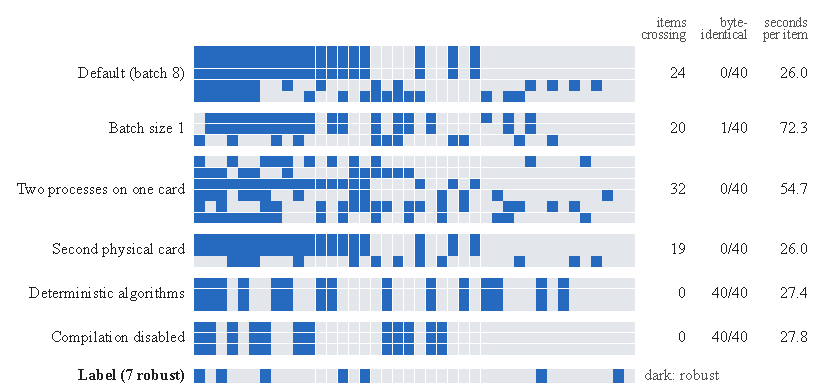
\includegraphics[width=\linewidth]{fig_rumore.pdf}
\caption{Predictions of the official pipeline for 40 preliminary public problems (columns) in 23 executions on DeepSeek (rows), by configuration; the last row is the label, dark cells are robust, and columns are sorted by how often they are predicted robust. At right: items whose prediction changes across the configuration's runs (more runs, more crossings), items whose generated text is byte-identical in all of them, and seconds per item.}
\label{fig:noise}
\end{figure}

\begin{table}[t]
\caption{Repeatability of the official pipeline on DeepSeek, 40 public problems, by configuration, in the order of Figure~\ref{fig:noise}. ``Crossings'': items whose prediction changes across the configuration's runs. ``Identical'': items whose generated text is byte-identical in all runs. Cost is runtime against the default configuration. Card 0 and card 1 are the two GPUs of the same machine. With two processes on one card, any five of its six runs give 29 to 31 crossings.}
\label{tab:reexec}
\centering
\small
\begin{tabular}{@{}lllllll@{}}
\toprule
\textbf{Configuration} & \textbf{Card} & \textbf{Runs} & \textbf{Crossings} & \textbf{Identical} & \textbf{Correct per run} & \textbf{Cost} \\
\midrule
Default (batch 8) & 0 & 5 & 24/40 & 0/40 & 24, 24, 24, 23, 24 & reference \\
Batch size 1 & 0 & 3 & 20/40 & 1/40 & 20, 21, 24 & +178\% \\
Two processes on one card & 0 & 6 & 32/40 & 0/40 & 24 to 28 & +110\% \\
Second physical card & 1 & 3 & 19/40 & 0/40 & 24, 24, 21 & +0\% \\
Deterministic algorithms & 0 & 3 & 0/40 & 40/40 & 24, 24, 24 & +5\% \\
Compilation disabled & 1 & 3 & 0/40 & 40/40 & 25, 25, 25 & +7\% \\
\bottomrule
\end{tabular}
\end{table}

\paragraph{Two candidate remedies.} Deterministic algorithms (PyTorch's, in warn-only mode, with deterministic cuDNN and a fixed cuBLAS workspace; Appendix~\ref{app:C}) and disabled compilation each made the generated text byte-identical in three sequential runs, at 5 to 7\% runtime cost. On card 0, the default configuration produced 24 crossings in five runs. Each remedy ran on one card where the default had produced crossings, each run in a new process, with no other process on that card. Three identical runs are weak evidence: the default configuration also gave three identical runs on card 0 before its fourth diverged, and five of its eight runs on the two cards shared one output. The two remedies produced different outputs, predicting 15 and 12 of the 40 problems robust, and because they ran on different cards we cannot tell whether the difference comes from the configuration or from the card. Neither gained more than one item (24 and 25 correct).

\paragraph{Distinct outputs.} The 23 executions fall into 14 distinct outputs, byte-identical within each. The same output appeared on both cards, and two runs launched in the same second on one card produced different outputs, so the output is not a property of the card alone; what selects it is not established. As only 7 of the 40 problems are robust and crossings largely cancel, accuracy moved much less than predictions: 21 to 24 correct in the default configuration on either card and 24 to 28 with two processes on one card, always below the 33 of the majority constant. An exploratory repetition of the official score extraction, whose third run ranks the 164 labeled problems at Spearman 0.24 against the first two, is in Appendix~\ref{app:C}.

\section{Regenerating the labels with our own protocol}\label{sec:labels}

\paragraph{Our labeling protocol.} We identified the organizers' perturbation families in the preliminary data (rephrase, rename, domain, distract, typos), regenerated them with gpt-oss-120b prompted with public examples, and gated each variant with gpt-oss-120b. An answer counts as correct when it matches gpt-oss-120b's answer on the original problem, because the preliminary data carry no answers; we did not check this key against the answers of the collections the problems come from. On the organizers' machine, with vLLM 0.28.0 [8] outside the official image, we labeled four models with two independent draws of variants (A and B, about 40 accepted variants per problem): 10 samples on the base problem and one per variant, at temperature 0.6, top-p 0.95 and at most 16,384 new tokens. Draw A's variants were also re-sampled with a new seed (A$'$). A label is robust when at least 6 of the 10 base samples are correct and every variant is answered correctly; unlike the earlier rule's conjunction, this requires the base problem to be solved.

A chain that reaches our cap is scored by the last boxed answer it contains, and counts as wrong without one; the organizers also count a response that reaches their limit without a parseable final answer as wrong [4]. Our protocol differs from the organizers' in perturbations, answer key, rule and sampling (one answer per variant, against 10 in the files behind most of their DeepSeek labels). Its decoding differs from the settings they publish, and its prompt may differ from the one behind their labels, which they have not stated.

\begin{table}[t]
\caption{Agreement of labels regenerated with our protocol: Cohen's kappa. The three columns for A and B treat variant chains that reached the 16,384-token cap in three ways: scored as in the protocol (by their last boxed answer, if any), dropped, or all counted as correct. The first of these columns and the A and A$'$ column give 95\% percentile bootstrap intervals over problems, and the script of Appendix~\ref{app:E} gives them for the other two. A problem has a label in a draw when it has at least one accepted variant (160 in A, 159 in B). Kappa between A and B uses the 159 problems labeled in both (150 for Qwen3.5-4B and 156 for DeepSeek when truncated chains are dropped), and between A and A$'$ 160. ``At cap'': percentage of variant chains that reached the cap in draws A and B. ``Robust'': percentage of problems labeled robust in draw A, as scored. The last column gives kappa of draw A with the organizers' preliminary DeepSeek labels: on the 138 published ones, and on the 160 that include 22 labels we derived (Section~\ref{sec:data}).}
\label{tab:label}
\centering
\small
\setlength{\tabcolsep}{3pt}
\begin{tabular}{@{}llllllll@{}}
\toprule
& & & \multicolumn{3}{l}{\textbf{A and B, truncated variant chains}} & & \\
\cmidrule(lr){4-6}
\textbf{Model} & \textbf{At cap} & \textbf{Robust} & \textbf{as scored} & \textbf{dropped} & \textbf{correct} & \textbf{A and A$'$} & \textbf{Organizers'} \\
\midrule
Skywork & 1.2, 1.5 & 74 & 0.44 [0.28, 0.59] & 0.39 & 0.39 & 0.79 [0.67, 0.89] & none \\
DeepSeek & 5.1, 6.1 & 39 & 0.41 [0.26, 0.55] & 0.35 & 0.36 & 0.46 [0.33, 0.59]$^{*}$ & 0.011; 0.025 \\
Olmo & 1.1, 0.9 & 68 & 0.38 [0.21, 0.54] & 0.39 & 0.39 & 0.65 [0.52, 0.78] & none \\
Qwen3.5-4B & 22.1, 29.2 & 9 & 0.18 [$-$0.06, 0.39] & 0.26 & 0.44 & not run & none \\
\bottomrule
\end{tabular}
\par\smallskip{\footnotesize $^{*}$On DeepSeek, A$'$ also received the answer-format line (end of this section), so this entry mixes seed and prompt.}
\end{table}

\paragraph{Results.} Under our protocol, two independent draws of variants give labels that agree at kappa 0.35 to 0.44 on Skywork, Olmo and DeepSeek, whether truncated variant chains are scored as in the protocol, dropped or all counted as correct (Table~\ref{tab:label}). On Qwen3.5-4B, 22 to 29\% of the variant chains reach the cap. Scoring these chains as in the protocol, dropping them or counting them all as correct gives agreement of 0.18, 0.26 and 0.44, and a robust share in draw A of 9\%, 83\% and 79\%. On Skywork, re-sampling the same variants with a new seed agrees far more than drawing new variants (0.79 against 0.44), so its label depends more on the variants than on the seed; on Olmo the gap is smaller (0.65 against 0.38), and on DeepSeek, where A$'$ also changed the prompt, it is 0.46 against 0.41.

Draw A's DeepSeek labels agree with the 138 labels the organizers published at kappa 0.011 [$-$0.13, 0.17], and with the 160 that include 22 of our derived labels at 0.025 [$-$0.12, 0.18]. Of the 36 problems with a published robust label, draw A calls 20 non-robust, and 4 of these change when truncated variants all count as correct. Of the 102 with a published non-robust label, draw A calls 44 robust. The reliability of the organizers' labels remains unmeasured. A retrospective calculation on the same saved answers with the main-phase threshold rule, applied as its pre-registration fixed it, with no filter on the base problem (Appendix~\ref{app:C}), gives test-retest point estimates between 0.34 and 0.56, below the pre-registered bar of 0.60, though three of the four intervals include it.

\paragraph{The prompt changes our labels.} In a first run with the bare problem text, later discarded, \mbox{Qwen3.5-4B} gave a final answer in the expected format in only 5 of its 1,640 base samples in draw A. With one instruction line requesting the format, 145 of 164 problems passed the base condition, against none. DeepSeek passed it on 147 of 164 with or without that line; its draws A and B ran without the line and A$'$ with it, and on the same variants its robust share moved from 39\% to 51\% of the 160 labeled problems, a change that mixes prompt and seed. Under our protocol, the label of Qwen3.5-4B therefore depends on the prompt. Whether this affects the organizers' labels is unknown: their baselines repository has a solve prompt that asks for an ANSWER line, but they have not said whether it was used for labeling (R3).

\section{The falsification campaign}\label{sec:campaign}

Table~\ref{tab:campaign} summarizes the campaign; Appendix~\ref{app:A} lists all 31 entries and explains three traps (rule T, the oracle H13, the duplicated pairs behind H2) and two pitfalls of the data. All entries use the preliminary data, except H16 to H18, which were scored on the 17 items of the warmup evaluation task.

\begin{table}[t]
\caption{The campaign in brief, in 19 of its 31 entries (Appendix~\ref{app:A} lists all). Ground truth is DeepSeek's and the preliminary pairs' unless stated; accuracy differences are in points against each pre-registration's baseline. H1, H7 and T count the 52 duplicated DeepSeek pairs twice; counted once, no verdict changes.}
\label{tab:campaign}
\centering
\small
\begin{tabular}{@{}L{5.5cm}L{1.9cm}L{5.6cm}@{}}
\toprule
\textbf{What we tested} & \textbf{Entries} & \textbf{Outcome} \\
\midrule
Text features; robustness as a property of the problem; labels, base accuracy and difficulty order across models & H1 to H5, H7 & rejected; H2 gained only when the duplicated pairs were counted twice \\
Official uncertainty features, logistic regression & H10 & 0.774 against a majority constant of 0.756, within the 0.692 $\pm$ 0.101 of the proposal [1] (method substituted) \\
Features cached for other models; per-target thresholds & H12, H13 & H12 rejected; the H13 ceiling withdrawn, $-$2.8 points when forced to rank \\
Our perturbation families, translation, self-consistency, the organizers' families regenerated (pilot), representation shift & H19, H22, H30 to H33 & rejected: kappa at most 0.02, AUROC at most 0.615 \\
Probes on DeepSeek's hidden states: ours and the organizers' published artifact & H36, H35 & survive their nulls; ours adds no detectable gain over length, and the artifact's score is probably in-sample \\
Trivial-robust rule, post hoc & T & a trap: +6.0 points on the preliminary pairs, +0.0 on \texttt{val-sample} \\
Identical bundles re-executed (warmup, 17 items) & H18 & noise confirmed: 11, 9, 11 and 11 correct \\
\bottomrule
\end{tabular}
\end{table}

\paragraph{Length and probes.} The character count of the problem alone orders the 164 DeepSeek labels at AUROC 0.704. Our logistic probe on DeepSeek's last-token hidden states, with layer and regularization chosen by inner cross-validation, reaches 0.710 out of fold with the original fold assignment. Over 20 other assignments, passed through the second-stage model below, it gives 0.57 to 0.76 (mean 0.69). Its scores correlate with length at Spearman +0.55, and residualized on log character count it gives 0.62. Its permutation null, rerun with 1{,}000 permutations of the whole nested procedure (the first version used 60, where 500 were pre-registered), gives $p = 0.002$. Restricted to the 138 published labels, these out-of-fold scores give 0.714 and length 0.733; retrained on those 138 alone with H36's procedure and seed, the probe gives 0.620. Combined with length in a second-stage model fitted on common outer folds, the probe changes AUROC over length alone by +0.005 on the 164 labels and by $-$0.010 on the 138 published ones (median bounds of the per-assignment 95\% intervals: $-$0.03 to 0.04, and $-$0.04 to 0.02): we detect no gain from adding the probe to length (Appendix~\ref{app:C}). This analysis replaces an earlier combination that leaked labels (Appendix~\ref{app:D}).

The organizers' published DeepSeek probe artifact orders the 164 DeepSeek labels at 0.739 with the aggregation we pre-registered and at 0.709 with its own, and at 0.62 and 0.57 residualized on log character count; its controls trained on shuffled labels give 0.68 at layer 31. The artifact does not record its training data; we infer that 137 of the 164 problems were among the public rows it was trained on, so these scores are probably largely in-sample. These length controls, which play the role of control tasks [7], were post hoc. Whether either probe reads anything beyond length that bears on robustness is not established. Apart from the three traps of Appendix~\ref{app:A}, no signal we scored by accuracy beats the majority constant by more than about one standard error on the preliminary labels, most of them DeepSeek's.

\section{Our entries}\label{sec:entries}

Our entry V8, pre-registered on 13 September, is the whole rule \texttt{return~[len(p)~>=~98 for~p~in~problems]}, with the threshold at the lower median of the 174 preliminary problems and the direction fixed on the preliminary pairs. On the original main-phase tasks it scored 11/21 and 10/19, like our entry v6 and the organizers' own entries. None of these beat the majority constant, which scores at least 11/21 and 10/19 on these tasks, and on so few items the ties do not show that length carries no signal (95\% Wilson intervals 0.32 to 0.72 and 0.32 to 0.73). On the 71 labeled rows of the official training set (revision of 17 September; 36 distinct problems), V8 differs from the all-robust constant on only 6 rows and is wrong on all 6 (46/71 against 52/71): too few to say what length is worth on official data. On the replacement tasks of 16 September, before and after the evaluation changed on 15 October [6], it predicted robust for every item (10/21 and 7/14), like an all-robust control. For the final test we nominated V8 (Codabench 1016713) and the constant (1016732), both on the Main track; our pre-registered predictions will be scored there (Appendix~\ref{app:B}).

\section{Recommendations}\label{sec:recs}

These rest mostly on DeepSeek and the preliminary data, and should be checked on the other models.
\begin{itemize}
\item \textbf{R1. Remove the variation between runs, and test the remedy:} on the same card with independent restarts, under load and across cards.
\item \textbf{R2. Repeat only where it decides something:} at the warmup's re-execution noise (a standard deviation of 1.0 item on 17, itself estimated from four runs), a one-item gap needs about eight runs per entry to reach two standard errors, so repeat only entries that run a model and sit near a prize boundary.
\item \textbf{R3. Say which prompt and decoding settings produced each released label file,} at least after the close.
\item \textbf{R4. Measure the label's reliability directly,} with two independent draws of variants labeled by the official process.
\item \textbf{R5. Show floors and noise on the leaderboard:} a row per constant predictor, the re-execution noise and binomial intervals.
\item \textbf{R6. Require a length control in white-box ablations.}
\item \textbf{R7. Remove the leaking field} \texttt{permutation\_type} from the aggregated datasets (Appendix~\ref{app:A}).
\end{itemize}

\paragraph{Code and data.} Our code, bundles, pre-registrations and outcome files are released at \href{https://github.com/Dan23RR/aimo-instrument}{\nolinkurl{github.com/Dan23RR/aimo-instrument}}. Its folder \texttt{reproduce/} recomputes the main tables from saved outputs and the six preliminary datasets, and the other numbers come from the dated records in \texttt{archive/} (Appendix~\ref{app:E}).

%%%%%% End of the main text: the six pages end here; the Limitations do not count %%%%%%
\label{fine-testo}

\section*{Limitations}

\begin{enumerate}[leftmargin=1.6em, itemsep=2pt, topsep=4pt, parsep=0pt]
\item \textbf{Preliminary data, not official data.} We did not repeat our label and probe analyses on the official training set, beyond the evaluation of V8 and a five-row check of our labels (Appendix~\ref{app:C}). Findings on label reliability and predictability may not generalize to the official evaluation setting.
\item \textbf{Our protocol, not the official one.} We did not regenerate labels with the organizers' published settings (100,000 tokens, temperature 1.0), with 10 answers per variant as in the files behind most DeepSeek labels, or on \texttt{train-main-v2}. The three treatments of truncated variant chains show how much our cap moves agreement between our draws; all three score base samples that reach the cap as the protocol does, and none of them reproduces longer decoding or a different temperature. Our low agreement with the organizers' labels is a fact about our process.
\item \textbf{One model.} We ran the probes, the re-execution study of Section~\ref{sec:reexec} and the comparisons of our regenerated labels with the organizers' preliminary labels only on DeepSeek.
\item \textbf{Re-execution.} We did not run the two candidate remedies on the same card, so card and configuration are confounded; we did not test either remedy under contention or on both cards, and we used 40 problems and one image.
\item \textbf{Records.} Some analyses rest on re-created scripts or dated records (Appendix~\ref{app:D}). Nothing here estimates performance on the final held-out problems.
\end{enumerate}

\section*{AI usage statement}

In this work, we used one generative AI tool, Claude (Anthropic), through Claude Code, for ideation, coding, analysis and writing. Ideation: it drafted the pre-registrations, including hypotheses, predictions and kill criteria, and searched and summarized the literature and the public records, including the organizers' Discord channels and the author's correspondence with them. Coding: it wrote the solution code of our bundles and the analysis and extraction scripts, ran them, and operated the organizers' virtual machine over SSH. Analysis: it computed and interpreted the results and ran automated adversarial reviews of hypotheses, drafts and code. Writing: it drafted the correspondence, this report and its revision after review.

It also made most of our Codabench uploads through the author's browser at the author's instruction. There were two exceptions: one resubmission (925822, 14 September), made without a specific instruction, and one submission that the author had not approved, sent in error and rejected before import (1016734, 28 October).

Language models were also components of our method: gpt-oss-120b generated and gated the perturbation variants and supplied the reference answers of Section~\ref{sec:labels}, and phi-4 translated problems for H22. The final decisions on the direction of the work, on the submissions (with the two exceptions above), on the nominations for the final test and on the claims of this report were the author's, and the author sent all correspondence personally. The author has reviewed all AI-assisted work and takes full responsibility for the final content of this report.

\begin{ack}
We thank Michal Štefánik, Róbert Belanec and the AIMO Interpretability team for the compute grant, a virtual machine with two GPUs, and for answering our questions; on 2 November they confirmed that the measurements taken on their machine may appear in this report. We also thank the three reviewers and the program chairs: two reviewers checked our analyses against the released code and data, and their checks corrected several of our claims. Other GPU time was rented on Modal and paid by the author or covered by Modal's platform credit. This work received no other funding, and the author has no competing interests.
\end{ack}

\section*{References}
{\small
[1] M. Štefánik, P. Mondorf, A. Waldis, Q. Liu, C. Yang, M. Spiegel, J. Kuchař, M. Kadlčík, A. Vawda-Oomerjee, C. Liu, S. Frieder, B. Plank, F. Barez and P. Stenetorp. AIMO Interpretability Challenge. CoRR, abs/2607.13899, 2026. doi:10.48550/arXiv.2607.13899.

[2] H. He and Thinking Machines Lab. Defeating Nondeterminism in LLM Inference. Thinking Machines Lab: Connectionism, 2025.

[3] J. Yuan, H. Li, X. Ding, W. Xie, Y.-J. Li, W. Zhao, K. Wan, J. Shi, X. Hu and Z. Liu. Understanding and Mitigating Numerical Sources of Nondeterminism in LLM Inference. NeurIPS 2025. arXiv:2506.09501.

[4] AIMO Interpretability Challenge website and FAQ. \url{https://aimo-interp.github.io} (accessed 28 October 2026), and its source repository aimo-interp/aimo-interp.github.io on GitHub.

[5] aimo-interp/getting-started and aimo-interp/baselines, GitHub repositories: README and issues \#6 and \#10 of getting-started; aimo-interp datasets on Hugging Face, including \texttt{train-main-v2} and \texttt{val-sample}.

[6] AIMO Interpretability Challenge Discord, \#announcements and \#qa: 5, 15 and 22 September, 9, 15, 16 and 20 October 2026.

[7] J. Hewitt and P. Liang. Designing and Interpreting Probes with Control Tasks. EMNLP-IJCNLP 2019.

[8] W. Kwon et al. Efficient Memory Management for Large Language Model Serving with PagedAttention. SOSP 2023.

[9] D. Hendrycks et al. Measuring Mathematical Problem Solving With the MATH Dataset. NeurIPS 2021 Datasets and Benchmarks Track. arXiv:2103.03874.
}

%%%%%% End of the references %%%%%%
\clearpage
\appendix
\raggedright

\section{The hypotheses, three traps and two pitfalls of the preliminary data}\label{app:A}

Section~\ref{sec:campaign} summarizes these entries. Unless stated, the ground truth is the 335 public pairs for H1 to H9 and T, the other models' preliminary labels for H12 to H15, the 17 items of the warmup evaluation set for H16 to H18, and DeepSeek's labels for the others. Validation that fits on some problems and tests on others is grouped by problem. The cross-model tests H7 and H12 to H15 hold out the model but not the problem, so part of them is in-sample; H7, H12, H14 and H15 were rejected anyway, and H13 is withdrawn. Numbers are accuracy points against each pre-registration's baseline unless they are kappa or AUROC.

{\small\setlength{\tabcolsep}{4pt}\renewcommand{\arraystretch}{1.2}
\begin{longtable}{L{1.1cm}L{3.9cm}L{5.6cm}L{2.0cm}}
\toprule
\textbf{ID} & \textbf{Hypothesis} & \textbf{Result} & \textbf{Verdict} \\
\midrule
\endfirsthead
\toprule
\textbf{ID} & \textbf{Hypothesis} & \textbf{Result} & \textbf{Verdict} \\
\midrule
\endhead
\bottomrule
\endlastfoot
H1 & The problem text predicts robustness (32 features) & 0.675 against 0.761, $-$8.7 ($-$7.4 with the duplicated pairs counted once) & rejected \\
H2 & Robustness is a property of the problem & with the 52 duplicated pairs counted once, z~=~0.88 and $-$1.3 against the per-model majority (bar 4.0); z~=~4.04 and +3.4 only when they are counted twice & rejected \\
H3 & One model's label predicts another's & $-$7.3 & rejected \\
H4 & One model's base accuracy predicts another's robustness & $-$11.8 & rejected \\
H5 & The difficulty order transfers across models & $-$25.4 & rejected \\
H6 & The same, with the oracle number of positives & $-$13.0 & ceiling (no kill criterion) \\
H7 & Base accuracy beats the prior on held-out models & $-$1.2 against the per-model majority that its pre-registration named (+0.0 against the global prior we used instead) & rejected \\
T & Robust if and only if base accuracy is below 0.05 (post hoc; see the traps below) & +6.0 on the 335 public pairs, +0.0 on \texttt{val-sample} & trap (no kill criterion) \\
H10 & The official uncertainty features reach the accuracy the proposal reports & 0.774 against a majority constant of 0.756, within 0.692 $\pm$ 0.101 [1]; a logistic regression on 13 of the 14 features of our own A100 re-implementation of the extraction (three of them constant), substituted for the official regressor & confirmed (method substituted, not declared at the time) \\
H11b & Length, saturation and trend features add signal & $-$1.8 and $-$2.5 & rejected \\
H12 & A cached model's uncertainty features predict other models & $-$16.5 & rejected \\
H13 & The same, with a threshold chosen per target & +7.3, from thresholds chosen on the scored items; $-$2.8 when forced to rank & withdrawn (no kill criterion) \\
H14, H15 & Calibration by the target's rate or by the global rate & $-$2.8 and $-$10.1 & rejected \\
H16 & Every model measured by itself beats the constant & 10/17 against 9/17 on one execution, inside the noise of H18 & survives, within noise \\
H17 & A gpt-oss threshold calibrated on \texttt{val-sample} beats H16 & 11/17, then 9, 11 and 11 on re-execution; 9/17 meets the kill criterion & not established \\
H18 & Identical bundles score differently across executions & 11, 9, 11 and 11 correct & confirmed (no kill criterion) \\
H19 & Our five mechanical perturbation families reproduce the organizers' preliminary label & accuracy 0.354 against 0.788, kappa 0.02 & rejected \\
H20 & A threshold tuned on our label transfers & 0.212 against 0.788 & rejected \\
H22 & Stability under translation reproduces the organizers' preliminary label & 0.507 against 0.740, kappa $-$0.10 & rejected \\
H23 & A threshold tuned on it transfers & +0.0 & rejected \\
H29 & Representation-distance features are repeatable (gate; written plan, not a frozen pre-registration) & ICC 0.997 to 0.999, from the dated outcome file & passes \\
H30 & The representation shift under perturbation predicts the label (written plan) & AUROC 0.615, below the kill threshold of 0.655; character count 0.704 (0.705 in E11's own computation) & rejected \\
H31 & The direction of that shift predicts the label (written plan) & AUROC 0.555 & rejected \\
H32 & The organizers' families, regenerated (pilot), reproduce their label & kappa $-$0.001 on four families, $-$0.030 with all five & rejected \\
H33 & Self-consistency over 8 samples predicts the label & AUROC 0.502 & rejected \\
H35 & The organizers' published probe artifact orders the 164 DeepSeek labels & 0.739 under the pre-registered aggregation and 0.709 under its own; 0.62 and 0.57 once residualized on log character count; its shuffled-label controls give 0.68 at layer 31 & survives its null; probably in-sample, not separated from length \\
H36 & Our linear probe, nested cross-validation, orders the 164 DeepSeek labels & 0.710 out of fold, above its permutation null, and 0.62 once residualized on log character count; 0.714 against 0.733 for length on the 138 published labels (Appendix~\ref{app:C}) & survives its null; no detectable gain over length \\
E13b-1 & Under the main-phase rule our regenerated label is test-retest reliable (kappa at least 0.60 on 3 of 4 models) & 0.34 to 0.56, retrospective (Appendix~\ref{app:C}) & rejected \\
E13b-2 & Under the main-phase rule it agrees with DeepSeek labels we computed with that rule from the preliminary data (kappa at least 0.40) & 0.02 [$-$0.09, 0.13] & rejected \\
E13b-3 & The labeling rule drives the instability of our regenerated labels & a gain of at least 0.15 on 2 of 4 models, where 3 were required; 0 of 4 on common problems & rejected \\
\end{longtable}
}

Not in the table are H8, H9, H21, H24 and H25 to H28. H8 is an oracle ceiling: 0.774, +1.8 points against the global constant and +0.4 against the per-model majority, with the duplicated pairs counted once. The outcome of H9 became rule T. H21 and H24 needed H19 and H20, and H22 and H23, to survive, so they were not run. H25 to H28 are entries of the E11 plan that its outcome file does not report under these identifiers. H25 is an anomaly of our own re-implementation of the extraction, found before the plan. H26 is the list field of the first pitfall below. H27 is a label-noise ceiling, which the plan itself closed with a resampling estimate instead of a test. H28 is the text-only baseline, which became character count (Appendix~\ref{app:D}). Three further E11 tests were not run (Appendix~\ref{app:D}). V4, an entry submitted once against its own pre-registered rule, is in Appendix~\ref{app:D}.

\paragraph{Three traps.} Rule T gains six points on the public pairs and nothing on \texttt{val-sample}, because the trivially robust items (base accuracy 0, robust under the conjunction) are absent there. The oracle H13 chose each target's threshold among all cut points on the very items it was scored on; forced to rank the items and to predict the true number of positives, it gave $-$2.8. H2 owed its survival to one measurement published under two model names and counted twice; counted once, its z falls from 4.04 to 0.88.

\paragraph{Two pitfalls of the preliminary data.} In the three aggregated datasets, the field \texttt{permutation\_type} is a list if and only if the item is robust, because the aggregation merges all perturbation types into one row for robust items and keeps one row per retained type otherwise, usually a single type. The rule ``robust if the field is a list'' reproduces all 223 labeled rows of the three datasets, and the field does not exist at inference (recommendation R7). And 20 of the 80 robust pairs among the 335 have base accuracy 0. None of them carries a published label, so they are robust only under the conjunction we used to derive their labels, while \texttt{val-sample} has no labeled pair with base accuracy below 0.05.

\section{Pre-registered predictions for the final evaluation}\label{app:B}

P1 was written on 7 September 2026, P-V8 on 13 September and P-V8b on 21 September. They are translated from the dated files and shortened. We omit the runtime predictions (under 60 seconds), which we could not score because the bundles log no runtime. A second prediction written with P1 on 7 September concerns another participant's final score and is not reported here.

\begin{itemize}
\item \textbf{P1.} The top-ranked entry's accuracy on the final held-out problems will lie within two binomial standard errors of that set's majority-class constant.
\item \textbf{P-V8.} If the organizers had neutralized length, V8 would score between 0.45 and 0.55 on both tracks (stated beforehand as the most likely outcome); if they had not, and the set was balanced, about 0.66. Observed on the original tasks: 0.52 and 0.53, inside the first band; on 21 and 19 items, however, 0.66 lies inside the 95\% intervals of both scores, so the scores do not exclude the second.
\item \textbf{P-V8b}, on the replacement tasks: the same bundles work with the new ingestion and score 6 to 15 of 21 and 4 to 10 of 14. Observed: coverage 1.0, no invalid predictions, 10/21 and 7/14, inside the bands but degenerately, since the rule predicted robust for every item.
\end{itemize}

\section{Protocols, run manifest and recalculations}\label{app:C}

\paragraph{Hardware and software.} The generation runs used the organizers' virtual machine with two NVIDIA RTX PRO 6000 Blackwell Server Edition GPUs (96 GB each), the evaluation workers' model, from 8 September 2026. Each run used one GPU; the Olmo-3-7B-Think A$'$ labels combine two runs, one on each card (below).
\begin{itemize}
\item \textbf{Official runtime image.} Section~\ref{sec:reexec} and the official score channel (E16) ran inside it: {\footnotesize\path{ghcr.io/aimo-interp/aimo-codabench-runtime:torch2.12.1-cuda13.2-cudnn9-transformers5.13.0-sklearn1.8.0-kernels0.15.2}}, digest {\footnotesize\path{sha256:fb4dab6343de7ce022ddd7906493f9ced16ff9008d497326a781d1e5adc8207a}}. They used the official extraction and regressor as shipped in our bundles: greedy decoding, at most 4,096 new tokens, static cache, batch 8.
\item \textbf{Labeling environment.} Section~\ref{sec:labels} ran with vLLM 0.28.0, torch 2.13.0 and transformers 5.16.1 (driver 610.57.04 with CUDA 13.3 on the machine, CUDA 13.0 runtime libraries in the environment) in a separate environment on the same machine; \texttt{vm\_backup/AMBIENTE\_VM\_2026-09-17.txt} lists every package.
\item \textbf{Model revisions.} Hugging Face snapshot hashes: Qwen3.5-4B \texttt{851bf6e8}, Skywork-OR1-Math-7B \texttt{fcef970f}, Olmo-3-7B-Think \texttt{d97e442d}, DeepSeek-R1-0528-Qwen3-8B \texttt{6e8885a6}, gpt-oss-120b \texttt{b5c939de}. The full hashes are in the run logs.
\item \textbf{Analyses.} They ran on CPU: E13's analysis and E15's evaluation, up to 14 September, on the virtual machine (Python 3.12, NumPy 2.3.5, scikit-learn 1.9.1), the others on the author's computer (Python 3.11.12, NumPy 2.4.4 and scikit-learn 1.8.0, as recorded for the runs of September and November). The release pins every output by SHA-256 in \texttt{MANIFEST.tsv}.
\end{itemize}

\needspace{8\baselineskip}
\paragraph{Run manifest.}
\begin{itemize}
\item \textbf{Where they ran.} The scripts in \texttt{vm/} written up to 14 September (setup, generation, extraction, E13's analysis and E15's evaluation), after which the machine stayed idle, and the clean-up script of 17 September ran on the virtual machine; the later ones ran on the author's computer.
\item \textbf{Outputs} are in \texttt{vm\_risultati/} unless the table gives another path.
\item \textbf{GPU-hours} are times from the logs (\texttt{reproduce/compute\_hours.py}). They include model loading except for the E13 labels, a difference under 1\%.
\end{itemize}

{\small\setlength{\tabcolsep}{4pt}
\begin{longtable}{L{2.4cm}L{3.2cm}L{2.2cm}>{\raggedright\arraybackslash\footnotesize}p{4.8cm}}
\toprule
\textbf{Run} & \textbf{Where it ran} & \textbf{GPU-hours} & \textbf{Outputs} \\
\midrule
\endfirsthead
\toprule
\textbf{Run} & \textbf{Where it ran} & \textbf{GPU-hours} & \textbf{Outputs} \\
\midrule
\endhead
\bottomrule
\endlastfoot
E13 variants & virtual machine & 1.15 and 1.20 & \path{e13/varianti_D1.parquet}, \path{e13/varianti_D2.parquet} \\
E13 labels & virtual machine, one queue per card & 64.4, in the logs of the 11 runs of Table~\ref{tab:label} & \path{e13/etich_*.parquet} \\
E13b, main-phase rule & author's computer & CPU only & \path{e13b_regola_nuova_2026-09-21.txt} \\
E14 re-execution & virtual machine, official image & 8.4 & \path{e14/out/*.jsonl}, \path{e14/log/} \\
E15 extraction & virtual machine & under 0.1 & \path{vm_backup/estratto/work/aimo/e15/hs_*.npz} \\
E15 probes & the virtual machine's CPU on 14 September, then the author's computer & CPU only & \path{e15_*}, \path{e15r/}, \path{vm_backup/estratto/work/aimo/e15_valuta.log} \\
E16 score channel & virtual machine, official image & 5.9 & \path{e16_*.jsonl}, \path{e16nodet/} \\
\end{longtable}
}

\paragraph{Commands.} Script paths are relative to \texttt{archive/}, the working folder of the repository. The scripts in \texttt{vm/} that ran on the virtual machine use paths under \texttt{/work/aimo}. \texttt{M} stands for the model, and in E14 \texttt{C}, \texttt{r}, \texttt{g} and \texttt{t} for the configuration, repetition, card and process tag.
\begin{itemize}
\item \textbf{E13 variants.} \texttt{vm/e13\_varianti.py -{}-draw~D1 -{}-seed~20260913 -{}-n~164 -{}-k~10}, and \texttt{-{}-draw~D2 -{}-seed~20260914}. The model gpt-oss-120b generates, solves and gates the variants (prompts below).
\item \textbf{E13 labels.} DeepSeek A and B ran an earlier version of \texttt{e13\_etichetta.py} that sent the bare problem text (now \texttt{-{}-prompt~nudo}); every other run behind Table~\ref{tab:label}, DeepSeek A$'$ included, used the explicit prompt. Draw A: \texttt{vm/e13\_etichetta.py -{}-model~M -{}-cond~A -{}-draw~D1 -{}-seed~20260921 -{}-prompt~esplicito}; B: \texttt{-{}-cond~B -{}-draw~D2 -{}-seed~20260922}; A$'$: \texttt{-{}-cond~Ap -{}-draw~D1 -{}-seed~20260923}. \texttt{vm/e13\_coda.sh} launched one queue per card (its logs are in \path{vm_backup/estratto/work/aimo/}); the card 0 queue ran an earlier version that passed no \texttt{-{}-prompt} flag, so DeepSeek A$'$ got the default of \texttt{e13\_etichetta.py}, the explicit prompt.
\item \textbf{E13b.} \texttt{vm/e13b\_regola\_nuova.py}, on the saved E13 answers; retrospective (below).
\item \textbf{E14.} \texttt{vm/e14\_all.sh 40 "C0 C1 C2 C3"} and \texttt{vm/e14\_extra.sh 1 "C5 C4"}. Each run is \texttt{e14\_run.py -{}-cond~C -{}-rep~r -{}-gpu~g -{}-tag~t -{}-n~40} inside the official image: 23 runs on DeepSeek. In the 8.4 GPU-hours the two processes of each contention pair, which shared one GPU, count once (20 runs).
\item \textbf{E15 extraction.} \texttt{vm/e15\_estrai.py -{}-model~deepseek-ai/DeepSeek-R1-0528-Qwen3-8B}, with and without the official system prompt: one forward pass per problem, last input token, all 37 hidden-state indices, at most 2,048 tokens.
\item \textbf{E15 probes.} \texttt{vm/e15\_valuta.py} ran H35, H36 and the first null (60 permutations) on 14 September, on the virtual machine's CPU; its log is \path{vm_backup/estratto/work/aimo/e15_valuta.log}. The file \path{vm_risultati/e15_valuta_2026-09-14.txt} is a later run of that day, by the file times in \path{vm_backup/MANIFEST_backup_aimo_2026-09-17.txt}, that stopped with an error at the null. H35's null is the 95th percentile, 0.602, of the AUROC of 20{,}000 random scores on the same labels, in either orientation. \texttt{vm/e15\_null\_nidificato.py} reran that null on 23 September with both grids of $C$, on the author's computer. E15-R (below) is \texttt{vm/e15r\_ricalcolo.py}, given an output folder and a number of worker processes (5 on the author's computer, 14.5 hours); its outputs are in \texttt{vm\_risultati/e15r}, and since it appends to existing files, a rerun needs a new folder. H35 needs the organizers' artifact \texttt{probe\_artifact.pkl} (hash below), which we do not redistribute.
\item \textbf{E16.} \texttt{vm/e16\_all.sh} and \texttt{vm/e16\_nodet.sh}, in the official image. Of the variables that \texttt{e16\_all.sh} sets, only the cuBLAS workspace variable reaches the extraction; \texttt{e16\_nodet.sh} sets neither.
\end{itemize}

The organizers' artifact used by H35 has SHA-256 {\footnotesize\texttt{8607478c7408922a6490adb7bda34d6a7d95403b7aa62f80dd3f2649139ccdeb}}. The listed logs total 82.8 GPU-hours. Not in the table:
\begin{itemize}
\item two complete runs of Qwen3.5-4B with the bare prompt (about 13 GPU-hours, no released log);
\item a partial run of Qwen3.5-4B A$'$ with the bare prompt (1.7 GPU-hours, included in the 82.8), discarded with them;
\item a run of Olmo-3-7B-Think A$'$ on card 1 (11.0 GPU-hours, 07:19 to 18:21 UTC on 10 September, from its queue log). Card 0 reached the same condition at 14:20, resumed from its partial file with 96 of the 164 problems done and finished the other 68, so the reported A$'$ labels come from both cards.
\end{itemize}
With these, the virtual machine ran about 107 GPU-hours, plus short smoke and feasibility tests. Our earlier runs on Modal used about 12 to 13 GPU-hours, mostly on A100 GPUs, as documented in their dated outcome files: the feature extraction behind H10, its pilot, and E9 to E12.

\paragraph{What can be recomputed.}
\begin{itemize}
\item \textbf{From saved outputs.} The scripts in \texttt{reproduce/} (Appendix~\ref{app:E}), which also read the six preliminary datasets; the other numbers come from the dated records in \texttt{archive/}.
\item \textbf{On a CPU, from the released hidden states.} Our probe (H36) and E15-R can be rerun end to end. H35 also needs the organizers' artifact.
\item \textbf{Only with the original GPUs and models.} The generation runs.
\end{itemize}

\paragraph{Re-execution configurations (Section~\ref{sec:reexec}).}
\begin{itemize}
\item \textbf{C0, default:} batch 8, on card 0, five runs.
\item \textbf{C1, batch size 1.}
\item \textbf{C2, deterministic algorithms:} \texttt{torch.use\_deterministic\_algorithms(True, warn\_only=True)}, \texttt{cudnn.deterministic = True}, \texttt{cudnn.benchmark = False} and \texttt{CUBLAS\_WORKSPACE\_CONFIG=:4096:8}.
\item \textbf{C3, contention:} two identical processes at the same time on card 0, three pairs.
\item \textbf{C4, second card:} the default on card 1.
\item \textbf{C5, compilation disabled:} \texttt{TORCH\_COMPILE\_DISABLE=1}, on card 1.
\end{itemize}
Runs within a configuration were sequential, each a new process. During these runs the other card was running another of our jobs. Two pre-registered predictions failed:
\begin{itemize}
\item batch size 1 did not make generation more repeatable: three runs gave three different outputs;
\item disabled compilation was predicted to land in one of the default outputs; it was byte-identical across its runs, but in an output of its own.
\end{itemize}
\texttt{reproduce/reexecution\_table.py} recomputes Table~\ref{tab:reexec} and the numbers of Figure~\ref{fig:noise}, and lists the 14 distinct outputs.

\paragraph{Variants and labels (Section~\ref{sec:labels}).}
\begin{itemize}
\item \textbf{Few-shot pool.} The generator saw five public examples of each family, drawn from a pool of 621 public examples (original, perturbed) over the five families. The texts are the organizers' and are not redistributed. \texttt{vm\_risultati/e13/fewshot\_pool\_ids.json} lists each example's problem identifier and SHA-256 hashes, and \texttt{reproduce/fewshot\_pool.py} rebuilds the pool from the downloaded preliminary datasets (verified on 23 November 2026: 621 of 621, byte-identical).
\item \textbf{Drawing the examples.} For draw seed $s$, problem $p$ and family $f$, the five examples are \texttt{random.Random("s|p|f").sample(pool[f] without p, 5)}.
\item \textbf{Generator.} gpt-oss-120b at low reasoning effort, temperature 1.0, top-p 1.0, at most 4,096 tokens, one request per problem and family, asking for 10 variants.
\item \textbf{Gate and reference answers.} gpt-oss-120b at medium effort, temperature 1.0, at most 8,192 tokens, solves the original and each variant. A variant is accepted if its text differs from the original, the length ratio lies between 0.7 and 4.0, and the solver's answer is unchanged. The solver's answer on the original is the reference answer.
\item \textbf{Labeling.}
  \begin{itemize}
  \item \textbf{Prompt.} Each model receives the instruction line (the second block below) followed by the problem, except DeepSeek in A and B, which received the bare text.
  \item \textbf{Sampling.} Temperature 0.6, top-p 0.95, at most 16,384 new tokens (raised from 8,192 before execution, after a test in which 2 of 3 problems saturated 8,192). There are 10 samples on the base problem and one per accepted variant.
  \item \textbf{Scoring.} A chain is scored by the last boxed answer it contains. Without one, including when it was cut at the cap, it counts as wrong.
  \end{itemize}
\end{itemize}

{\footnotesize
Generator prompt:
\begin{quote}\ttfamily
You create variants of mathematics competition problems for a robustness benchmark. Perturbation type: <family>. <family instruction> The variant must be a complete, self-contained problem with exactly the same final answer as the original. Do not solve the problem. Do not add hints or solutions. Here are 5 examples of this perturbation type: Example 1 Original: <public original> Variant: <public variant> (four more examples) Now write 10 different variants of the following problem. Make them genuinely different from each other. Output each variant between <variant> and </variant> tags, and nothing else. Original: <problem>
\end{quote}
Instruction line of the labeling prompt, also used by the solver of the gate:
\begin{quote}\ttfamily
Solve the following problem. Reason step by step, then give only the final answer inside \textbackslash{}boxed\{\}.
\end{quote}
}
The five family instructions, verbatim:
\begin{itemize}
\item rephrase: ``Rewrite the problem in different words while preserving exactly its mathematical content and its final answer.''
\item rename: ``Rename the variables, people, objects or entities in the problem while preserving its mathematical structure and its final answer.''
\item domain: ``Transfer the problem to a different real-world surface domain (a different story, setting and objects) while preserving exactly the same mathematical structure and the same final answer.''
\item distract: ``Insert irrelevant but plausible additional information (extra facts, numbers or context) that does not change the problem or its final answer.''
\item typos: ``Introduce harmless typographical or formatting noise (misspellings, spacing, punctuation, capitalisation) without changing the meaning of the problem or its final answer.''
\end{itemize}

\paragraph{The main-phase rule, retrospectively (E13b).} PREREG\_E13b was written on 21 September, before any calculation under the main-phase rule but after the E13 answers had been measured, so the calculation is retrospective.
\begin{itemize}
\item \textbf{The rule.} On the saved answers, a problem is robust if the largest drop in accuracy across families is at most 0.10 and non-robust if it is at least 0.25; problems in between get no label.
\item \textbf{No base filter.} As pre-registered, the primary calculation has no filter on the base problem, so a problem the model never solves counts as robust when no family lowers its accuracy.
\item \textbf{Test-retest, primary.} Kappa between A and B is 0.34 [0.13, 0.53] on 86 problems (Qwen3.5-4B), 0.49 [0.17, 0.76] on 132 (Skywork), 0.41 [0.09, 0.69] on 133 (Olmo) and 0.56 [0.36, 0.73] on 100 (DeepSeek). Because 58 to 95\% of the problems are labeled robust, kappa stays low even where raw agreement is high.
\item \textbf{Test-retest, secondary (S1).} On problems with at least 5 of 10 correct base samples in both draws, kappa is 0.31, 0.52, 0.40 and 0.55.
\item \textbf{Against the organizers.} Against DeepSeek labels that we computed with the same rule from the accuracy drops published in the preliminary data: 0.02 [$-$0.09, 0.13] on 133 problems.
\item \textbf{Against \texttt{train-main-v2}.} On its five labeled rows that fall on our problems and models, our labels agree with the official ones on 2 (draw A, one undefined) and 3 (draw B); five rows are too few to read.
\item \textbf{Truncated chains} are scored as in the protocol here too.
\end{itemize}

\paragraph{Subsampling (E13).} Subsampling DeepSeek's variants from 2 to 40 per problem leaves the mean kappa between A and B between 0.36 and 0.47, with no upward trend: more variants per problem do not make our labels more repeatable.

\paragraph{The official score channel (E16, exploratory).} We extracted the official regressor score on DeepSeek three times for the 174 public problems with the same code and image; this measurement was not pre-registered. The first run set the cuBLAS workspace variable and gave the same scores as the second, run without it, on all 174 problems. The second and third correlate at Spearman 0.24 over the 164 labeled problems. They give AUROC 0.487 and 0.602 in the regressor's own orientation; the paired bootstrap 95\% interval of their difference, $-$0.015 to 0.246, includes zero. The ranking of the problems was not reproduced in one of two repetitions; this does not show that the signal itself changes. As 137 of the 164 problems are in the regressor's training set, this concerns the stability of its inputs, not new problems. The 5.9 GPU-hours of the manifest also include one extraction each on Qwen3.5-4B, Skywork and Olmo, which this report does not use, and a failed start on gpt-oss-120b.

\paragraph{E15-R: the probe recalculated after review.} The procedure was fixed in \texttt{vm/e15r\_ricalcolo.py} before it ran, in a run started on 23 November 2026. It uses the same hidden states, labels and nested cross-validation as H36: layers 1 to 36, $C$ in \{0.001, 0.01, 0.1, 1\}, 5 outer and 4 inner folds.
\begin{itemize}
\item \textbf{Combination with length.}
  \begin{itemize}
  \item There are 20 fold assignments on the 164 labels and 10 on the 138 published ones.
  \item The probe's scores for the outer training problems come from a nested cross-validation inside them. Its score for each outer test problem comes from a probe selected and fitted on the outer training problems.
  \item A second-stage logistic regression on log character count, on the probe score, or on both, is fitted on the outer training problems and scored on the outer test problems.
  \item The 95\% interval of the gain of ``both'' over length is a paired bootstrap over problems (2,000 resamples) for each assignment; we report the median of its bounds.
  \end{itemize}
\item \textbf{Retraining.} The nested probe is retrained on the 138 published labels alone.
\item \textbf{Permutation null.} The null of H36 is extended from 60 to 1,000 permutations of the whole nested procedure, with the seeds of the first 60 unchanged.
\end{itemize}
We fixed the decision rule before the run: if the interval of the gain includes zero, the probe adds nothing measurable to length.

\begin{center}
\small
\begin{tabular}{@{}lllll@{}}
\toprule
\textbf{Labels} & \textbf{Length} & \textbf{Probe} & \textbf{Both} & \textbf{Gain of both over length} \\
\midrule
164 (20 assignments) & 0.696 & 0.692 & 0.701 & +0.005 [$-$0.03, 0.04] \\
138 published (10 assignments) & 0.729 & 0.644 & 0.720 & $-$0.010 [$-$0.04, 0.02] \\
\bottomrule
\end{tabular}
\end{center}
Values are means over the assignments. Length and probe here are the second-stage models, cross-validated and pooled over folds, so they differ slightly from the raw values of Section~\ref{sec:campaign} (0.704 and 0.733 for character count). On the 164 labels the gain ranges from $-$0.024 to +0.023 over the 20 assignments, and its interval excludes zero in 1 of them; the probe's second-stage model alone ranges from 0.57 to 0.76. The inner cross-validation chose hidden-state index 4 in 66 of the 100 outer folds. On the 138 published labels the gain ranges from $-$0.026 to +0.012 over the 10 assignments. With H36's procedure and random seed, the probe retrained on the 138 published labels alone gives AUROC 0.620, against 0.733 for character count; the probe's second-stage model of the table ranges from 0.59 to 0.71 over its 10 assignments.

The null with 1{,}000 permutations has mean 0.4975 and 95th percentile 0.6032; 1 permutation reaches the observed 0.710 ($p = 0.002$). Its first 60 permutations reproduce the null of 23 September (mean 0.4890, 95th percentile 0.5700) to the last digit. The run stopped after 925 permutations, when the computer restarted; \texttt{vm/e15r\_riprendi.py} computed the other 75 with the same permutations and seeds.

\section{Withdrawn claims, deviations and records}\label{app:D}

\paragraph{Claims withdrawn after review.}
\begin{itemize}
\item \textbf{A bound on latent agreement.} We had corrected the kappa of 0.025 with the organizers' DeepSeek labels for our own noise and quoted about 0.27 as an upper bound on latent agreement. That needs a measurement-error model for binary labels that we had not justified.
\item \textbf{The combination of probe and length.} Its earlier second-stage cross-validation reused probe scores computed on other folds, so some training scores depended on test labels. Its numbers (0.696 for length, 0.697 for the probe, 0.714 for both) are replaced by E15-R (Appendix~\ref{app:C}).
\item \textbf{Re-execution.} We no longer infer that the output of a run is fixed when the process starts.
\item \textbf{A simulation.} A plug-in simulation of the organizers' labeling process, which we had reported as overstating test-retest agreement by about 0.4, is no longer reported. It was a model of their process, not a measurement of it.
\end{itemize}
The other changes after review are listed in the repository README.

\paragraph{Deviations from the pre-registrations.} Each pre-registration is dated before execution, and the deviations below are also recorded as notes in those files.
\begin{itemize}
\item \textbf{Not pre-registered.} E5 is documented only in its outcome file. E11 ran from a written plan without the frozen pre-registration it called for. E16 was not pre-registered, although we had told the organizers that every experiment on their machine would be.
\item \textbf{E4.} H7 was compared with the global prior of the training models instead of the pre-registered per-model majority, against which it scores $-$1.2 points.
\item \textbf{E6.} H10 was run as a logistic regression on 13 of the 14 features in place of the pre-registered regressor and threshold, and this was not declared at the time.
\item \textbf{E11.}
  \begin{itemize}
  \item Three planned primary tests were not run.
  \item A Holm correction was planned and not applied, and H30 would fail it.
  \item The confirmation set was not held out.
  \item AUROCs were computed on raw scores, with the orientation chosen on the data.
  \item Only one of the three planned layer depths (0.80, the primary one) was extracted.
  \item The six-feature text baseline of H28 was replaced by character count alone, and the two reference analyses the plan required next to every AUROC were not computed.
  \end{itemize}
\item \textbf{E13.}
  \begin{itemize}
  \item gpt-oss-120b was pre-registered for labeling and not labeled.
  \item DeepSeek's A$'$ received the answer-format line through a queueing error.
  \item The pre-registered table that mapped outcomes to readings was not followed, because it assumed our regeneration reproduces the organizers' process.
  \item The subsampling curve varied the variants per problem, where the design varied them per family.
  \item The token cap was raised from 8,192 to 16,384 before execution.
  \end{itemize}
\item \textbf{E13b.} It was written after the E13 answers had been measured (Appendix~\ref{app:C}).
\item \textbf{E14.} Its fourth measure, the repeatability (ICC) of the 14 official features, was not computed, and two of its predictions failed (Appendix~\ref{app:C}).
\item \textbf{E15.}
  \begin{itemize}
  \item It predicted that both probes would fail their nulls; both survived.
  \item H36's nested null was pre-registered with 500 permutations and the full grid of $C$. The first run (14 September) used 60 permutations and two values of $C$. It was rerun with the full grid on 23 September, and extended to 1{,}000 permutations in a run started on 23 November.
  \item The Holm correction over the two primaries was not computed.
  \item The length controls of H35 and H36 were post hoc.
  \end{itemize}
\item \textbf{V4.} The allocation entry (909843) predicted robust on the 9 warmup items of gpt-oss-120b. It combined three numbers: the share of robust items implied by public leaderboard scores of constant entries, the count of gpt-oss-120b items read from the log of our warmup submission 907310, and that model's higher robust rate in the preliminary datasets (0.40 against 0.24). Our compliance review found that without the first two, which describe the evaluation set, it reduces to the entry it modified. Its pre-registration said it would not be sent if that review refuted it; the review did, and the author submitted it once anyway, as a measurement kept off the leaderboard. It tied the entry it modified.
\end{itemize}

\paragraph{Records.} Several analyses were first run from scripts that were not saved, and were re-created and saved later. The two length-control scripts of E15 and the rerun of its null were re-created on 23 September, each checked against the logged values before use. A few figures rest only on a dated record, not on a saved per-item output: H29's repeatability, the GPU-hours on Modal, and V8's predictions on the replacement and current tasks, which come from counts its container logged.

\paragraph{Earlier corrections.} Between our first drafts and the submitted version we corrected 54 of our own statements. They are listed, with what each changed, in \texttt{CORRECTIONS.md} in the repository, and every number in this report already includes them. The main text cites English entry points (\texttt{reproduce/}); the commands of the run manifest keep the original script names, which the dated pre-registrations cite.

\section{Data, assets, release and submissions}\label{app:E}

\paragraph{Data.}
\begin{itemize}
\item \textbf{Preliminary datasets.} The six datasets published by the organizers under \texttt{aimo-interp} on Hugging Face before the main phase: \texttt{val-sample}, \texttt{augmented-sample-math}, \texttt{augmented-sample-math-full-filtered}, \texttt{augmented-sample-math-agg-filtered}, \texttt{aimo-interp-challenge-sample-full} and \texttt{augmented-sample-math-agg}. Their cards state no license. Their problems come from the MATH dataset [9] and from the AIMO 2025 reference problems, as their \texttt{dataset\_id} field records.
\item \textbf{Official training set.} \texttt{train-main-v2} at revision 23791d9 of 17 September 2026 (82 rows, 71 labeled; the organizers extended it to 94 rows on 15 October). Its card states the license as ``other''.
\item \textbf{Downloading.} \texttt{dati.py} downloads the six preliminary datasets; we do not redistribute copies of the organizers' datasets. Our analyses used the files below. Their SHA-256 values begin as follows, and \texttt{reproduce/README.md} gives them in full.

\smallskip
{\small\begin{tabular}{@{}ll@{}}
\texttt{aimo-interp-challenge-sample-full} & \texttt{b8a57039} \\
\texttt{val-sample} & \texttt{afae22a0} \\
\texttt{augmented-sample-math-agg} & \texttt{3d168c29} \\
\texttt{augmented-sample-math-agg-filtered} & \texttt{a96bf90d} \\
\texttt{augmented-sample-math} & \texttt{991b74c0} \\
\texttt{augmented-sample-math-full-filtered} & \texttt{1b62215f} \\
\end{tabular}}
\end{itemize}

\paragraph{Models and code.} The models used, with their licenses:
\begin{itemize}
\item gpt-oss-120b (OpenAI, Apache-2.0);
\item Olmo-3-7B-Think, and Olmo-3-7B-Instruct of the warmup evaluation set (Allen Institute for AI, Apache-2.0);
\item DeepSeek-R1-0528-Qwen3-8B (DeepSeek, MIT);
\item Qwen3.5-4B (Qwen, Apache-2.0);
\item Skywork-OR1-Math-7B (Skywork; no license stated on its card);
\item phi-4 (Microsoft, MIT), for the translations of H22;
\item gemma-3-27b-it (Google, Gemma Terms of Use), loaded by our warmup entries for H16 to H18.
\end{itemize}
From the organizers we used the evaluation harness, the official uncertainty-feature extraction with its DeepSeek regressor, and the DeepSeek probe artifact with its inference code (\texttt{aimo-interp/getting-started}, which states no license); from \texttt{aimo-interp/baselines} (Apache-2.0) we used three files [5]. vLLM [8] (Apache-2.0) ran the generation, gating and labeling of Section~\ref{sec:labels}.

\paragraph{Release.} In \href{https://github.com/Dan23RR/aimo-instrument}{\nolinkurl{github.com/Dan23RR/aimo-instrument}}, the folder \texttt{archive/} keeps the layout of our working folder, with the dated records gathered in \texttt{archive/records/}. The file paths cited in this report are relative to \texttt{archive/}, except \texttt{reproduce/}, \texttt{MANIFEST.tsv} and \texttt{CORRECTIONS.md}, which sit at the top of the repository next to \texttt{paper/}, this report's sources.
\begin{itemize}
\item \textbf{Contents.} The pre-registrations, outcome files, analysis scripts, extraction outputs (including the hidden states of E15), our perturbation variants, and our submission bundles as submitted. Our code is under the MIT license, and our contribution to the data under CC BY 4.0.
\item \textbf{Organizers' files.} The getting-started files inside our bundles and our variants are released with the organizers' permission of 2 November 2026. In our variant files, the rows of the original problems keep their identifiers but not their texts. Five original problems of \texttt{val-sample} remain, as submitted, in the calibration file of the v6 bundles.
\item \textbf{Not released.} Copies of the organizers' datasets, phi-4's translations of the problems (H22), the texts of the few-shot pool (\texttt{reproduce/fewshot\_pool.py} rebuilds them), our correspondence and our internal notes. Other participants' names and passages about their entries are redacted.
\end{itemize}

{\small\setlength{\tabcolsep}{4pt}
\begin{longtable}{L{3.7cm}L{6.2cm}L{3.0cm}}
\toprule
\textbf{Script in \texttt{reproduce/}} & \textbf{What it recomputes} & \textbf{Runs on} \\
\midrule
\endfirsthead
\toprule
\textbf{Script in \texttt{reproduce/}} & \textbf{What it recomputes} & \textbf{Runs on} \\
\midrule
\endhead
\bottomrule
\endlastfoot
\texttt{labels\_table.py} & Table~\ref{tab:label} and the agreement numbers of Section~\ref{sec:labels} & saved E13 answers, seconds \\
\texttt{reexecution\_table.py} & Table~\ref{tab:reexec}, the numbers of Figure~\ref{fig:noise} and the 14 outputs of Section~\ref{sec:reexec} & saved E14 outputs, seconds \\
\texttt{probe\_vs\_length.py} & the probe and length AUROCs of Section~\ref{sec:campaign}; it prints the E15-R results and computes the permutation p-value from the saved null & saved E15 outputs, seconds \\
\texttt{v8\_threshold.py} & the two parameters of V8 (Section~\ref{sec:entries}) & public datasets, seconds \\
\texttt{compute\_hours.py} & the GPU-hours of Appendix~\ref{app:C} & logs, seconds \\
\texttt{fewshot\_pool.py} & the few-shot pool of the variant generator & public datasets, seconds \\
\end{longtable}
}

\paragraph{Italian words in file names.} The scripts and folders keep their original names, which the dated pre-registrations cite. The Italian words in the names printed in this report mean:

{\small\setlength{\tabcolsep}{6pt}
\begin{tabular}{@{}llll@{}}
\toprule
\textbf{Word} & \textbf{Meaning} & \textbf{Word} & \textbf{Meaning} \\
\midrule
\texttt{dati} & data & \texttt{nidificato} & nested \\
\texttt{risultati} & results & \texttt{nudo}, \texttt{esplicito} & bare, explicit (prompt) \\
\texttt{varianti} & variants & \texttt{regola\_nuova} & new rule \\
\texttt{etichetta}, \texttt{etich} & label & \texttt{ricalcolo} & recalculation \\
\texttt{coda} & queue & \texttt{riprendi} & resume \\
\texttt{valuta} & evaluate & \texttt{costante} & constant \\
\texttt{estrai}, \texttt{estratto} & extract, extracted & \texttt{ambiente} & environment \\
\texttt{sonde} & probes (here, bundles) & & \\
\bottomrule
\end{tabular}}

\paragraph{Codabench submissions.} These are all our submissions in both phases (user \texttt{dan23rr}), read from the Codabench API on 28 October 2026; accuracy is items correct over items.
\begin{itemize}
\item \textbf{Warmup, 29 to 31 August.} Our warmup entries are 907310, 907677, 907967, 909567, 909843, 909853, 909976, 909994, 910002 and 910013. They include a constant floor (907310), the official baseline instrumented only to log its runtime (907677), and V4, the allocation entry (909843; Appendix~\ref{app:D}). The four executions of v6 (H17, H18) gave 11, 9, 11 and 11 of 17.
\item \textbf{Original main-phase tasks.}
  \begin{itemize}
  \item 912096 and 912097 are v6, the measuring entry: 11/21 and 10/19.
  \item 924969 and 924974 are V8: 11/21 and 10/19.
  \item Their parents 924968 and 924972 also produced two rejected children (924970 and 924973) and six cancelled ones.
  \item 925822 is V8 again, uploaded by the AI assistant without a specific instruction.
  \end{itemize}
\item \textbf{Replacement tasks.} 936802 and 936806 are V8: 10/21 and 7/14.
\item \textbf{Current tasks, 28 October.}
  \begin{itemize}
  \item 1016713 and 1016730 are V8, unchanged: 10/21 and 7/14.
  \item 1016732 and 1016735 are the all-robust constant: 10/21 and 7/14.
  \item 1016733 is the parent that sent the constant's Small bundle to both tasks; its child 1016734, on the Main task, was sent in error and rejected before import.
  \end{itemize}
\item \textbf{Nominated for the final test.} 1016713 and 1016732, both on the Main track.
\end{itemize}

\needspace{6\baselineskip}
\paragraph{Bundles.} Neither nominated bundle loads a model or reads data at run time. V8's two parameters were fixed on the six preliminary datasets, its only training data, and \texttt{reproduce/v8\_threshold.py} recomputes them. The bundles are in \texttt{sonde/}. The SHA-256 of each:
\begin{itemize}
\item \texttt{solution-v8-main.zip}, a single \texttt{solution.py} with the rule of Section~\ref{sec:entries}: {\footnotesize\texttt{7b70f15c51752dcf4285e477d58c541d0ecf052d833c325c0702dbbd054ffb5f}};
\item \texttt{solution-v8-small.zip}, the same with the marker file \texttt{small.txt}: {\footnotesize\texttt{0b83b55f94dc16b9852a7c2b35d71ac5787e43d81afd6396dee00fb5e011e500}};
\item \texttt{solution-costante-main.zip}, the all-robust constant: {\footnotesize\texttt{35c47bbef717a5d4c5b6c7786bddbab9d87a02483e4f417cd34fd4ecf669c67d}};
\item \texttt{solution-costante-small.zip}, the same with \texttt{small.txt}: {\footnotesize\texttt{f798c2979b136a84c22e6d994bf0228bbfeffa044ac68f7868e13859b4c6075a}}.
\end{itemize}
To reproduce our score, upload the Main bundle to task 36237 and the Small bundle to task 36241, each with only its own task selected. On the current validation tasks the expected results are 10/21 and 7/14.


\newpage
\section*{NeurIPS Paper Checklist}




\begin{enumerate}

\item {\bf Claims}
    \item[] Question: Do the main claims made in the abstract and introduction accurately reflect the paper's contributions and scope?
    \item[] Answer: \answerYes{}
    \item[] Justification: The abstract and Section 1 state the three results and their scope: the re-execution measurement on DeepSeek, labels regenerated with our own protocol, which is not the official one, and hypotheses tested mostly on DeepSeek with the preliminary public data. The Scope paragraph of Section 1 states these limits before the results.
    \item[] Guidelines:
    \begin{itemize}
        \item The answer \answerNA{} means that the abstract and introduction do not include the claims made in the paper.
        \item The abstract and/or introduction should clearly state the claims made, including the contributions made in the paper and important assumptions and limitations. A \answerNo{} or \answerNA{} answer to this question will not be perceived well by the reviewers. 
        \item The claims made should match theoretical and experimental results, and reflect how much the results can be expected to generalize to other settings. 
        \item It is fine to include aspirational goals as motivation as long as it is clear that these goals are not attained by the paper. 
    \end{itemize}

\item {\bf Limitations}
    \item[] Question: Does the paper discuss the limitations of the work performed by the authors?
    \item[] Answer: \answerYes{}
    \item[] Justification: The Limitations section after Section 7 states what we did not do: repeat the analyses on the official data, regenerate labels with the organizers' settings, run them on other models, or test the remedies under more conditions. Sections 3 to 5 qualify each result where it is stated, and Appendix D lists the withdrawn claims and the deviations from the pre-registrations.
    \item[] Guidelines:
    \begin{itemize}
        \item The answer \answerNA{} means that the paper has no limitation while the answer \answerNo{} means that the paper has limitations, but those are not discussed in the paper. 
        \item The authors are encouraged to create a separate ``Limitations'' section in their paper.
        \item The paper should point out any strong assumptions and how robust the results are to violations of these assumptions (e.g., independence assumptions, noiseless settings, model well-specification, asymptotic approximations only holding locally). The authors should reflect on how these assumptions might be violated in practice and what the implications would be.
        \item The authors should reflect on the scope of the claims made, e.g., if the approach was only tested on a few datasets or with a few runs. In general, empirical results often depend on implicit assumptions, which should be articulated.
        \item The authors should reflect on the factors that influence the performance of the approach. For example, a facial recognition algorithm may perform poorly when image resolution is low or images are taken in low lighting. Or a speech-to-text system might not be used reliably to provide closed captions for online lectures because it fails to handle technical jargon.
        \item The authors should discuss the computational efficiency of the proposed algorithms and how they scale with dataset size.
        \item If applicable, the authors should discuss possible limitations of their approach to address problems of privacy and fairness.
        \item While the authors might fear that complete honesty about limitations might be used by reviewers as grounds for rejection, a worse outcome might be that reviewers discover limitations that aren't acknowledged in the paper. The authors should use their best judgment and recognize that individual actions in favor of transparency play an important role in developing norms that preserve the integrity of the community. Reviewers will be specifically instructed to not penalize honesty concerning limitations.
    \end{itemize}

\item {\bf Theory assumptions and proofs}
    \item[] Question: For each theoretical result, does the paper provide the full set of assumptions and a complete (and correct) proof?
    \item[] Answer: \answerNA{}
    \item[] Justification: The paper has no theoretical results.
    \item[] Guidelines:
    \begin{itemize}
        \item The answer \answerNA{} means that the paper does not include theoretical results. 
        \item All the theorems, formulas, and proofs in the paper should be numbered and cross-referenced.
        \item All assumptions should be clearly stated or referenced in the statement of any theorems.
        \item The proofs can either appear in the main paper or the supplemental material, but if they appear in the supplemental material, the authors are encouraged to provide a short proof sketch to provide intuition. 
        \item Inversely, any informal proof provided in the core of the paper should be complemented by formal proofs provided in appendix or supplemental material.
        \item Theorems and Lemmas that the proof relies upon should be properly referenced. 
    \end{itemize}

    \item {\bf Experimental result reproducibility}
    \item[] Question: Does the paper fully disclose all the information needed to reproduce the main experimental results of the paper to the extent that it affects the main claims and/or conclusions of the paper (regardless of whether the code and data are provided or not)?
    \item[] Answer: \answerYes{}
    \item[] Justification: Sections 2 to 6 and Appendix C describe the data, procedures, hardware, runtime image, model revisions, configurations, prompts and decision rules. Appendix C gives the run manifest with commands and GPU-hours, Appendix D lists the deviations from the pre-registrations, and Appendix E explains how to reproduce our score.
    \item[] Guidelines:
    \begin{itemize}
        \item The answer \answerNA{} means that the paper does not include experiments.
        \item If the paper includes experiments, a \answerNo{} answer to this question will not be perceived well by the reviewers: Making the paper reproducible is important, regardless of whether the code and data are provided or not.
        \item If the contribution is a dataset and\slash or model, the authors should describe the steps taken to make their results reproducible or verifiable. 
        \item Depending on the contribution, reproducibility can be accomplished in various ways. For example, if the contribution is a novel architecture, describing the architecture fully might suffice, or if the contribution is a specific model and empirical evaluation, it may be necessary to either make it possible for others to replicate the model with the same dataset, or provide access to the model. In general. releasing code and data is often one good way to accomplish this, but reproducibility can also be provided via detailed instructions for how to replicate the results, access to a hosted model (e.g., in the case of a large language model), releasing of a model checkpoint, or other means that are appropriate to the research performed.
        \item While NeurIPS does not require releasing code, the conference does require all submissions to provide some reasonable avenue for reproducibility, which may depend on the nature of the contribution. For example
        \begin{enumerate}
            \item If the contribution is primarily a new algorithm, the paper should make it clear how to reproduce that algorithm.
            \item If the contribution is primarily a new model architecture, the paper should describe the architecture clearly and fully.
            \item If the contribution is a new model (e.g., a large language model), then there should either be a way to access this model for reproducing the results or a way to reproduce the model (e.g., with an open-source dataset or instructions for how to construct the dataset).
            \item We recognize that reproducibility may be tricky in some cases, in which case authors are welcome to describe the particular way they provide for reproducibility. In the case of closed-source models, it may be that access to the model is limited in some way (e.g., to registered users), but it should be possible for other researchers to have some path to reproducing or verifying the results.
        \end{enumerate}
    \end{itemize}


\item {\bf Open access to data and code}
    \item[] Question: Does the paper provide open access to the data and code, with sufficient instructions to faithfully reproduce the main experimental results, as described in supplemental material?
    \item[] Answer: \answerYes{}
    \item[] Justification: Our scripts, pre-registrations, outcome files, extraction outputs, bundles and variants are public at \url{https://github.com/Dan23RR/aimo-instrument} (Section 7 and Appendix E). Its folder \texttt{reproduce/} recomputes Tables 1 and 2, the numbers of Figure 1, the probe and length AUROCs, the parameters of V8, the GPU-hours and the few-shot pool from saved outputs and the six preliminary datasets. The organizers' datasets are downloaded by \texttt{archive/dati.py} rather than redistributed.
    \item[] Guidelines:
    \begin{itemize}
        \item The answer \answerNA{} means that paper does not include experiments requiring code.
        \item Please see the NeurIPS code and data submission guidelines (\url{https://neurips.cc/public/guides/CodeSubmissionPolicy}) for more details.
        \item While we encourage the release of code and data, we understand that this might not be possible, so \answerNo{} is an acceptable answer. Papers cannot be rejected simply for not including code, unless this is central to the contribution (e.g., for a new open-source benchmark).
        \item The instructions should contain the exact command and environment needed to run to reproduce the results. See the NeurIPS code and data submission guidelines (\url{https://neurips.cc/public/guides/CodeSubmissionPolicy}) for more details.
        \item The authors should provide instructions on data access and preparation, including how to access the raw data, preprocessed data, intermediate data, and generated data, etc.
        \item The authors should provide scripts to reproduce all experimental results for the new proposed method and baselines. If only a subset of experiments are reproducible, they should state which ones are omitted from the script and why.
        \item At submission time, to preserve anonymity, the authors should release anonymized versions (if applicable).
        \item Providing as much information as possible in supplemental material (appended to the paper) is recommended, but including URLs to data and code is permitted.
    \end{itemize}


\item {\bf Experimental setting/details}
    \item[] Question: Does the paper specify all the training and test details (e.g., data splits, hyperparameters, how they were chosen, type of optimizer) necessary to understand the results?
    \item[] Answer: \answerYes{}
    \item[] Justification: Appendix A gives the data splits and the grouping by problem, and Sections 5 and 6 the thresholds and how they were chosen. Section 5 and Appendix C give the probe's nested cross-validation, Section 4 and Appendix C the decoding, sampling, seeds and token cap of the regeneration, and Section 3 and Appendix C the re-execution configurations.
    \item[] Guidelines:
    \begin{itemize}
        \item The answer \answerNA{} means that the paper does not include experiments.
        \item The experimental setting should be presented in the core of the paper to a level of detail that is necessary to appreciate the results and make sense of them.
        \item The full details can be provided either with the code, in appendix, or as supplemental material.
    \end{itemize}

\item {\bf Experiment statistical significance}
    \item[] Question: Does the paper report error bars suitably and correctly defined or other appropriate information about the statistical significance of the experiments?
    \item[] Answer: \answerYes{}
    \item[] Justification: We report 95\% percentile bootstrap intervals over problems for the agreement statistics (Section 4, Table 2 and Appendix C) and Wilson intervals for V8's scores (Section 6). Appendix C adds a paired bootstrap interval for the official score channel and an interval for the gain of the probe combined with length; Section 5 and Appendix C give the permutation nulls for the probes. The accuracy differences of Appendix A carry no intervals.
    \item[] Guidelines:
    \begin{itemize}
        \item The answer \answerNA{} means that the paper does not include experiments.
        \item The authors should answer \answerYes{} if the results are accompanied by error bars, confidence intervals, or statistical significance tests, at least for the experiments that support the main claims of the paper.
        \item The factors of variability that the error bars are capturing should be clearly stated (for example, train/test split, initialization, random drawing of some parameter, or overall run with given experimental conditions).
        \item The method for calculating the error bars should be explained (closed form formula, call to a library function, bootstrap, etc.)
        \item The assumptions made should be given (e.g., Normally distributed errors).
        \item It should be clear whether the error bar is the standard deviation or the standard error of the mean.
        \item It is OK to report 1-sigma error bars, but one should state it. The authors should preferably report a 2-sigma error bar than state that they have a 96\% CI, if the hypothesis of Normality of errors is not verified.
        \item For asymmetric distributions, the authors should be careful not to show in tables or figures symmetric error bars that would yield results that are out of range (e.g., negative error rates).
        \item If error bars are reported in tables or plots, the authors should explain in the text how they were calculated and reference the corresponding figures or tables in the text.
    \end{itemize}

\item {\bf Experiments compute resources}
    \item[] Question: For each experiment, does the paper provide sufficient information on the computer resources (type of compute workers, memory, time of execution) needed to reproduce the experiments?
    \item[] Answer: \answerYes{}
    \item[] Justification: Appendix C gives the hardware (two NVIDIA RTX PRO 6000 Blackwell Server Edition GPUs with 96 GB each, on the organizers' virtual machine), the runtime image and the GPU-hours of every main run from its logs (82.8 in the released logs, about 107 with the discarded runs and the card-1 run of Olmo-3-7B-Think A$'$), the GPU-hours on Modal and the CPU time of the probe recalculation; Figure 1 gives the seconds per item of each configuration.
    \item[] Guidelines:
    \begin{itemize}
        \item The answer \answerNA{} means that the paper does not include experiments.
        \item The paper should indicate the type of compute workers CPU or GPU, internal cluster, or cloud provider, including relevant memory and storage.
        \item The paper should provide the amount of compute required for each of the individual experimental runs as well as estimate the total compute. 
        \item The paper should disclose whether the full research project required more compute than the experiments reported in the paper (e.g., preliminary or failed experiments that didn't make it into the paper). 
    \end{itemize}
    
\item {\bf Code of ethics}
    \item[] Question: Does the research conducted in the paper conform, in every respect, with the NeurIPS Code of Ethics \url{https://neurips.cc/public/EthicsGuidelines}?
    \item[] Answer: \answerYes{}
    \item[] Justification: The work analyses public benchmark data and our own submissions; the release also includes pseudonymized snapshots of the public leaderboard. It involves no human-subjects research and makes no claim about other participants' methods, and the released files have other participants' names and passages about their entries removed (Appendix E). The organizers confirmed on 2 November that the measurements taken on their virtual machine may appear in this report.
    \item[] Guidelines:
    \begin{itemize}
        \item The answer \answerNA{} means that the authors have not reviewed the NeurIPS Code of Ethics.
        \item If the authors answer \answerNo, they should explain the special circumstances that require a deviation from the Code of Ethics.
        \item The authors should make sure to preserve anonymity (e.g., if there is a special consideration due to laws or regulations in their jurisdiction).
    \end{itemize}


\item {\bf Broader impacts}
    \item[] Question: Does the paper discuss both potential positive societal impacts and negative societal impacts of the work performed?
    \item[] Answer: \answerNo{}
    \item[] Justification: The paper does not discuss societal impacts: it measures re-execution noise in a competition's evaluation pipeline and the behavior of labels regenerated with our own protocol, and its recommendations concern evaluation practice (Section 7). The ways it documents to obtain misleading scores, a field that leaks the label in development data and re-execution noise, come with the fixes we recommend (R1, R2, R5 and R7).
    \item[] Guidelines:
    \begin{itemize}
        \item The answer \answerNA{} means that there is no societal impact of the work performed.
        \item If the authors answer \answerNA{} or \answerNo, they should explain why their work has no societal impact or why the paper does not address societal impact.
        \item Examples of negative societal impacts include potential malicious or unintended uses (e.g., disinformation, generating fake profiles, surveillance), fairness considerations (e.g., deployment of technologies that could make decisions that unfairly impact specific groups), privacy considerations, and security considerations.
        \item The conference expects that many papers will be foundational research and not tied to particular applications, let alone deployments. However, if there is a direct path to any negative applications, the authors should point it out. For example, it is legitimate to point out that an improvement in the quality of generative models could be used to generate Deepfakes for disinformation. On the other hand, it is not needed to point out that a generic algorithm for optimizing neural networks could enable people to train models that generate Deepfakes faster.
        \item The authors should consider possible harms that could arise when the technology is being used as intended and functioning correctly, harms that could arise when the technology is being used as intended but gives incorrect results, and harms following from (intentional or unintentional) misuse of the technology.
        \item If there are negative societal impacts, the authors could also discuss possible mitigation strategies (e.g., gated release of models, providing defenses in addition to attacks, mechanisms for monitoring misuse, mechanisms to monitor how a system learns from feedback over time, improving the efficiency and accessibility of ML).
    \end{itemize}
    
\item {\bf Safeguards}
    \item[] Question: Does the paper describe safeguards that have been put in place for responsible release of data or models that have a high risk for misuse (e.g., pre-trained language models, image generators, or scraped datasets)?
    \item[] Answer: \answerNA{}
    \item[] Justification: We release no models and no data with a high risk of misuse. The release (Appendix E) consists of our scripts and their outputs, our labels and per-variant answers, the hidden states of one public model on public problems, our submission bundles as submitted and, with the organizers' permission, perturbed versions of public math problems.
    \item[] Guidelines:
    \begin{itemize}
        \item The answer \answerNA{} means that the paper poses no such risks.
        \item Released models that have a high risk for misuse or dual-use should be released with necessary safeguards to allow for controlled use of the model, for example by requiring that users adhere to usage guidelines or restrictions to access the model or implementing safety filters. 
        \item Datasets that have been scraped from the Internet could pose safety risks. The authors should describe how they avoided releasing unsafe images.
        \item We recognize that providing effective safeguards is challenging, and many papers do not require this, but we encourage authors to take this into account and make a best faith effort.
    \end{itemize}

\item {\bf Licenses for existing assets}
    \item[] Question: Are the creators or original owners of assets (e.g., code, data, models), used in the paper, properly credited and are the license and terms of use explicitly mentioned and properly respected?
    \item[] Answer: \answerYes{}
    \item[] Justification: Appendix E credits the models, the datasets with the sources of their problems and the revision we used, and the code we used, with the licenses stated on their pages; where no license is stated, we say so. The organizers allowed the redistribution of their files inside our bundles and of our variants on 2 November.
    \item[] Guidelines:
    \begin{itemize}
        \item The answer \answerNA{} means that the paper does not use existing assets.
        \item The authors should cite the original paper that produced the code package or dataset.
        \item The authors should state which version of the asset is used and, if possible, include a URL.
        \item The name of the license (e.g., CC-BY 4.0) should be included for each asset.
        \item For scraped data from a particular source (e.g., website), the copyright and terms of service of that source should be provided.
        \item If assets are released, the license, copyright information, and terms of use in the package should be provided. For popular datasets, \url{paperswithcode.com/datasets} has curated licenses for some datasets. Their licensing guide can help determine the license of a dataset.
        \item For existing datasets that are re-packaged, both the original license and the license of the derived asset (if it has changed) should be provided.
        \item If this information is not available online, the authors are encouraged to reach out to the asset's creators.
    \end{itemize}

\item {\bf New assets}
    \item[] Question: Are new assets introduced in the paper well documented and is the documentation provided alongside the assets?
    \item[] Answer: \answerYes{}
    \item[] Justification: Our variants, labels, extraction outputs, analysis scripts and bundles are released at \url{https://github.com/Dan23RR/aimo-instrument} (Appendix E), with the dated pre-registrations and outcome files, a README, a manifest of SHA-256 hashes and licenses (MIT for our code, CC BY 4.0 for our contribution to the data).
    \item[] Guidelines:
    \begin{itemize}
        \item The answer \answerNA{} means that the paper does not release new assets.
        \item Researchers should communicate the details of the dataset\slash code\slash model as part of their submissions via structured templates. This includes details about training, license, limitations, etc. 
        \item The paper should discuss whether and how consent was obtained from people whose asset is used.
        \item At submission time, remember to anonymize your assets (if applicable). You can either create an anonymized URL or include an anonymized zip file.
    \end{itemize}

\item {\bf Crowdsourcing and research with human subjects}
    \item[] Question: For crowdsourcing experiments and research with human subjects, does the paper include the full text of instructions given to participants and screenshots, if applicable, as well as details about compensation (if any)? 
    \item[] Answer: \answerNA{}
    \item[] Justification: The paper involves no crowdsourcing and no research with human subjects.
    \item[] Guidelines:
    \begin{itemize}
        \item The answer \answerNA{} means that the paper does not involve crowdsourcing nor research with human subjects.
        \item Including this information in the supplemental material is fine, but if the main contribution of the paper involves human subjects, then as much detail as possible should be included in the main paper. 
        \item According to the NeurIPS Code of Ethics, workers involved in data collection, curation, or other labor should be paid at least the minimum wage in the country of the data collector. 
    \end{itemize}

\item {\bf Institutional review board (IRB) approvals or equivalent for research with human subjects}
    \item[] Question: Does the paper describe potential risks incurred by study participants, whether such risks were disclosed to the subjects, and whether Institutional Review Board (IRB) approvals (or an equivalent approval/review based on the requirements of your country or institution) were obtained?
    \item[] Answer: \answerNA{}
    \item[] Justification: The paper involves no human subjects.
    \item[] Guidelines:
    \begin{itemize}
        \item The answer \answerNA{} means that the paper does not involve crowdsourcing nor research with human subjects.
        \item Depending on the country in which research is conducted, IRB approval (or equivalent) may be required for any human subjects research. If you obtained IRB approval, you should clearly state this in the paper. 
        \item We recognize that the procedures for this may vary significantly between institutions and locations, and we expect authors to adhere to the NeurIPS Code of Ethics and the guidelines for their institution. 
        \item For initial submissions, do not include any information that would break anonymity (if applicable), such as the institution conducting the review.
    \end{itemize}

\item {\bf Declaration of LLM usage}
    \item[] Question: Does the paper describe the usage of LLMs if it is an important, original, or non-standard component of the core methods in this research? Note that if the LLM is used only for writing, editing, or formatting purposes and does \emph{not} impact the core methodology, scientific rigor, or originality of the research, declaration is not required.
    %this research? 
    \item[] Answer: \answerYes{}
    \item[] Justification: Language models are the objects of study (Section 2). In our label regeneration gpt-oss-120b generated and gated the perturbation variants and supplied the reference answers (Section 4, Appendix C), and phi-4 translated problems for H22 (Appendix A). An AI assistant (Claude, through Claude Code) drafted the pre-registrations, wrote and ran the code, operated the virtual machine, made most of our uploads and drafted this report and its revision, as disclosed in the AI usage statement.
    \item[] Guidelines:
    \begin{itemize}
        \item The answer \answerNA{} means that the core method development in this research does not involve LLMs as any important, original, or non-standard components.
        \item Please refer to our LLM policy in the NeurIPS handbook for what should or should not be described.
    \end{itemize}

\end{enumerate}

\end{document}
".
%% Every line numbered (same numbering, used to find the lines cited in the note): "\def\everyline{}\documentclass{article}

%% Conditional revision of November 2026: six pages of main text, from the title to the end of Section 7 (label
%% fine-testo); the Limitations, the AI usage statement, the references and the appendices do not count.
%% Final mode with the workshop name. Line numbers on every fifth line, small and grey, for the note to the
%% program chairs, who asked for section and line numbers. Copy without them: pdflatex "\def\cleancopy{}\documentclass{article}

%% Conditional revision of November 2026: six pages of main text, from the title to the end of Section 7 (label
%% fine-testo); the Limitations, the AI usage statement, the references and the appendices do not count.
%% Final mode with the workshop name. Line numbers on every fifth line, small and grey, for the note to the
%% program chairs, who asked for section and line numbers. Copy without them: pdflatex "\def\cleancopy{}\documentclass{article}

%% Conditional revision of November 2026: six pages of main text, from the title to the end of Section 7 (label
%% fine-testo); the Limitations, the AI usage statement, the references and the appendices do not count.
%% Final mode with the workshop name. Line numbers on every fifth line, small and grey, for the note to the
%% program chairs, who asked for section and line numbers. Copy without them: pdflatex "\def\cleancopy{}\input{main}".
%% Every line numbered (same numbering, used to find the lines cited in the note): "\def\everyline{}\input{main}".
\usepackage[final,sglblindworkshop]{neurips_2026}
\workshoptitle{AIMO Interpretability Challenge}
\ifdefined\cleancopy\else
  \usepackage{lineno}
  \linenumbers
  \ifdefined\everyline\else\modulolinenumbers[5]\fi
  \renewcommand\linenumberfont{\normalfont\tiny\sffamily\color{black!45}}
\fi

\usepackage[utf8]{inputenc}
\usepackage[T1]{fontenc}
%% Typewriter text in Latin Modern, the Type 1 version of the default Computer Modern typewriter, with the same
%% widths: without it, \texttt in T1 encoding becomes bitmap (Type 3) fonts, and the template asks for Type 1 fonts.
\renewcommand{\ttdefault}{lmtt}
\usepackage{hyperref}
\hypersetup{pdftitle={The Instrument Behind the Leaderboard: Re-Execution Noise and Label Regeneration in the AIMO Interpretability Challenge}, pdfauthor={Daniel Culotta}}
\usepackage{url}
\def\UrlBreaks{\do\/\do\.\do\_\do\-\do\:}
\usepackage{booktabs}
\usepackage{array}
\usepackage{longtable}
\newcolumntype{L}[1]{>{\raggedright\arraybackslash}p{#1}}
\usepackage{amsfonts}
\usepackage{microtype}
\usepackage{xcolor}
\usepackage{graphicx}
\usepackage{enumitem}
\usepackage{needspace}
\setlist[itemize]{leftmargin=1.4em, itemsep=2pt, topsep=4pt, parsep=0pt}
\setlist[itemize,2]{label=$\circ$}
\renewcommand{\arraystretch}{1.15}
\raggedbottom

\title{The Instrument Behind the Leaderboard: Re-Execution Noise and Label Regeneration in the AIMO Interpretability Challenge}

\author{%
  Daniel Culotta \\
  Independent researcher
}

\begin{document}

\maketitle

\begin{abstract}
We treat the AIMO Interpretability benchmark, which asks whether a model's answer to a math problem survives perturbations, as a measurement instrument. Almost all our label and probe analyses use the preliminary datasets. As the program chairs note, these differ from the official training and validation data in sampling, perturbations and eligibility, so findings on label reliability and predictability may not hold in the official evaluation. First, on DeepSeek-R1-0528-Qwen3-8B in the official pipeline, 24 of 40 items changed prediction across five default runs. Turning compilation off, or deterministic algorithms on, gave three byte-identical runs, each on one card. Second, we regenerated labels with our own protocol, not the official one: our perturbations and answer key, one answer per variant, a 16,384-token cap and temperature 0.6, where the organizers publish 100,000 tokens and 1.0. Two independent draws agree at kappa 0.35 to 0.44 on three of four models however truncated chains are treated, and 0.18 to 0.44 on Qwen3.5-4B, whose chains often reach the cap. Draw A agrees with the 138 published DeepSeek labels at kappa 0.01. This describes our protocol and does not measure the reliability of the organizers' labels. Third, of the 27 dated hypotheses with a kill criterion, 21 failed it. Our probe on DeepSeek's hidden states does no better than problem length (AUROC 0.710 against 0.704; below length on the published labels) and adds nothing detectable to it.
\end{abstract}

\section{Introduction}\label{sec:1}

A leaderboard is a measurement. Its score is read off an instrument made of a label, an evaluation set, an inference pipeline and the hardware it runs on. When the label is itself produced by a stochastic process, the instrument has noise of its own, which a single submission cannot see. We measure the re-execution noise of the official extraction and regressor, and the repeatability of labels regenerated with our own protocol, not the noise of the organizers' labels.

We study the instrument of the AIMO Interpretability Challenge, in which a submission predicts, for a given model and math problem, whether the model's answer is robust to perturbations of the problem [1]. We ran our work as a falsification campaign: every hypothesis was recorded in a dated file, 26 of the 31 before their data were seen, and every tested hypothesis is reported. Of the 31 entries, 27 carried a kill criterion written before their test ran (for 3 of them in a written plan rather than a frozen pre-registration, and for H2 after its concordance had been seen). By that criterion 21 were rejected, 5 survived and 1 is not established (Appendix~\ref{app:A}).

\paragraph{Scope.} Three limits apply.
\begin{itemize}
\item \textbf{Preliminary and official data.} Almost all of our label and probe analyses use the six preliminary public datasets released before the main phase. Their labels follow an earlier rule than those of the official training set (\texttt{train-main-v2}) and of the validation and test tasks [5]; as the program chairs noted in their meta-review, their sampling procedures, perturbations and eligibility criteria also differ. Beyond the label rule, we did not compare the two. Unless we say otherwise, a result on labels or on their predictability holds for the preliminary data and may not hold in the official evaluation setting.
\item \textbf{Our labeling protocol is not the official one.} When we regenerate labels (Section~\ref{sec:labels}), we use our own perturbations, prompts, sampling, decoding, answer key and labeling rule. Disagreement with the organizers' preliminary labels therefore shows that the two processes give different labels; it does not establish that their labels are unreliable or irreproducible.
\item \textbf{Mostly one model.} The re-execution study of Section~\ref{sec:reexec}, the probe analyses and every comparison of our regenerated labels with the organizers' preliminary labels are on DeepSeek-R1-0528-Qwen3-8B. Regenerated labels cover four models, but no conclusion about the official benchmark is established across models.
\end{itemize}

Within these limits, Sections~\ref{sec:reexec} to~\ref{sec:campaign} report re-execution noise and two candidate remedies, our regenerated labels, and signals that do no better than problem length or come from an artifact of the data. Nondeterminism of LLM inference is documented in general [2, 3]; we add its size for one model, one submission and 40 problems on this benchmark's hardware and pipeline. We make no claim about any participant's method.

\section{The task, the labels and the data}\label{sec:data}

\paragraph{Task.} A submission receives a model identifier, a reasoning effort and a list of problems, and returns one robustness verdict per problem, offline on one GPU within one hour [4, 5], or 70 minutes since 15 October [6]. The models are Qwen3.5-4B, Skywork-OR1-Math-7B, Olmo-3-7B-Think and \mbox{DeepSeek-R1-0528-Qwen3-8B} in both tracks, and gpt-oss-120b in the Main track only.

\paragraph{Official data.} The main-phase training set \texttt{train-main-v2} labels all five models with a threshold on the largest accuracy drop across perturbation families: robust at most 0.10, non-robust at least 0.25, no label in between [5]. The organizers' published decoding settings are up to 100,000 tokens at temperature 1.0, top-k 40 and top-p 0.95, and a response that reaches the limit without a final answer counts as wrong [4]. Since 16 September the private validation tasks have 21 items (Main) and 14 (Small), on which the binomial standard error of an accuracy near one half is 10.9 and 13.4 points; the final test uses 30 to 50 new problems [5, 6].

\paragraph{Preliminary data.} Six datasets released before the main phase aggregate to 335 (model, problem) pairs over 174 distinct problems, up to eight per problem; 52 pairs repeat the DeepSeek measurements under a second model name. Their labels follow an earlier rule: on all 379 labeled rows (a pair can have several), the label equals the conjunction ``no perturbation lowered accuracy''. A per-family majority rule (``more than half of the answers are correct in every perturbation family'') reproduces the same 379 labels, so these rows cannot tell the two rules apart. Whether they used the decoding settings above is not documented; in the files behind most DeepSeek labels, most variants listed as lowering accuracy were answered 10 times. We call their labels the organizers' preliminary labels, and keep ``official'' for \texttt{train-main-v2} and the validation and test tasks.

\paragraph{DeepSeek labels.} DeepSeek is the only evaluated model with many preliminary labels: 164 distinct problems (the 52 duplicated pairs count once). For 138 of them the data publish a label. For the other 26 we derived one with the conjunction, which makes 4 of them robust; the majority rule would make 21 robust, so these 26 labels depend on the choice of rule. We therefore report results on the 138 published labels separately.

\section{Re-execution noise on the evaluation workers' type of GPU}\label{sec:reexec}

On a virtual machine lent by the organizers, with two NVIDIA RTX PRO 6000 Blackwell Server Edition GPUs (the type the evaluation workers use), we ran 40 preliminary public problems through the official runtime image, extraction and regressor, unmodified, on DeepSeek. Decoding was greedy, with at most 4,096 new tokens in batches of 8. The 40 labels are DeepSeek's of Section~\ref{sec:data}: 28 published and 12 that we derived with the conjunction, which include 3 of the 7 robust ones. Figure~\ref{fig:noise} shows the 23 executions; Table~\ref{tab:reexec} gives the repeatability of each configuration.

\begin{figure}[t]
\centering
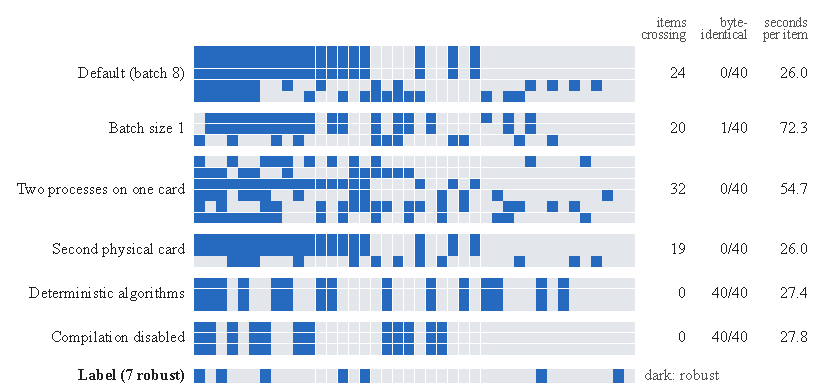
\includegraphics[width=\linewidth]{fig_rumore.pdf}
\caption{Predictions of the official pipeline for 40 preliminary public problems (columns) in 23 executions on DeepSeek (rows), by configuration; the last row is the label, dark cells are robust, and columns are sorted by how often they are predicted robust. At right: items whose prediction changes across the configuration's runs (more runs, more crossings), items whose generated text is byte-identical in all of them, and seconds per item.}
\label{fig:noise}
\end{figure}

\begin{table}[t]
\caption{Repeatability of the official pipeline on DeepSeek, 40 public problems, by configuration, in the order of Figure~\ref{fig:noise}. ``Crossings'': items whose prediction changes across the configuration's runs. ``Identical'': items whose generated text is byte-identical in all runs. Cost is runtime against the default configuration. Card 0 and card 1 are the two GPUs of the same machine. With two processes on one card, any five of its six runs give 29 to 31 crossings.}
\label{tab:reexec}
\centering
\small
\begin{tabular}{@{}lllllll@{}}
\toprule
\textbf{Configuration} & \textbf{Card} & \textbf{Runs} & \textbf{Crossings} & \textbf{Identical} & \textbf{Correct per run} & \textbf{Cost} \\
\midrule
Default (batch 8) & 0 & 5 & 24/40 & 0/40 & 24, 24, 24, 23, 24 & reference \\
Batch size 1 & 0 & 3 & 20/40 & 1/40 & 20, 21, 24 & +178\% \\
Two processes on one card & 0 & 6 & 32/40 & 0/40 & 24 to 28 & +110\% \\
Second physical card & 1 & 3 & 19/40 & 0/40 & 24, 24, 21 & +0\% \\
Deterministic algorithms & 0 & 3 & 0/40 & 40/40 & 24, 24, 24 & +5\% \\
Compilation disabled & 1 & 3 & 0/40 & 40/40 & 25, 25, 25 & +7\% \\
\bottomrule
\end{tabular}
\end{table}

\paragraph{Two candidate remedies.} Deterministic algorithms (PyTorch's, in warn-only mode, with deterministic cuDNN and a fixed cuBLAS workspace; Appendix~\ref{app:C}) and disabled compilation each made the generated text byte-identical in three sequential runs, at 5 to 7\% runtime cost. On card 0, the default configuration produced 24 crossings in five runs. Each remedy ran on one card where the default had produced crossings, each run in a new process, with no other process on that card. Three identical runs are weak evidence: the default configuration also gave three identical runs on card 0 before its fourth diverged, and five of its eight runs on the two cards shared one output. The two remedies produced different outputs, predicting 15 and 12 of the 40 problems robust, and because they ran on different cards we cannot tell whether the difference comes from the configuration or from the card. Neither gained more than one item (24 and 25 correct).

\paragraph{Distinct outputs.} The 23 executions fall into 14 distinct outputs, byte-identical within each. The same output appeared on both cards, and two runs launched in the same second on one card produced different outputs, so the output is not a property of the card alone; what selects it is not established. As only 7 of the 40 problems are robust and crossings largely cancel, accuracy moved much less than predictions: 21 to 24 correct in the default configuration on either card and 24 to 28 with two processes on one card, always below the 33 of the majority constant. An exploratory repetition of the official score extraction, whose third run ranks the 164 labeled problems at Spearman 0.24 against the first two, is in Appendix~\ref{app:C}.

\section{Regenerating the labels with our own protocol}\label{sec:labels}

\paragraph{Our labeling protocol.} We identified the organizers' perturbation families in the preliminary data (rephrase, rename, domain, distract, typos), regenerated them with gpt-oss-120b prompted with public examples, and gated each variant with gpt-oss-120b. An answer counts as correct when it matches gpt-oss-120b's answer on the original problem, because the preliminary data carry no answers; we did not check this key against the answers of the collections the problems come from. On the organizers' machine, with vLLM 0.28.0 [8] outside the official image, we labeled four models with two independent draws of variants (A and B, about 40 accepted variants per problem): 10 samples on the base problem and one per variant, at temperature 0.6, top-p 0.95 and at most 16,384 new tokens. Draw A's variants were also re-sampled with a new seed (A$'$). A label is robust when at least 6 of the 10 base samples are correct and every variant is answered correctly; unlike the earlier rule's conjunction, this requires the base problem to be solved.

A chain that reaches our cap is scored by the last boxed answer it contains, and counts as wrong without one; the organizers also count a response that reaches their limit without a parseable final answer as wrong [4]. Our protocol differs from the organizers' in perturbations, answer key, rule and sampling (one answer per variant, against 10 in the files behind most of their DeepSeek labels). Its decoding differs from the settings they publish, and its prompt may differ from the one behind their labels, which they have not stated.

\begin{table}[t]
\caption{Agreement of labels regenerated with our protocol: Cohen's kappa. The three columns for A and B treat variant chains that reached the 16,384-token cap in three ways: scored as in the protocol (by their last boxed answer, if any), dropped, or all counted as correct. The first of these columns and the A and A$'$ column give 95\% percentile bootstrap intervals over problems, and the script of Appendix~\ref{app:E} gives them for the other two. A problem has a label in a draw when it has at least one accepted variant (160 in A, 159 in B). Kappa between A and B uses the 159 problems labeled in both (150 for Qwen3.5-4B and 156 for DeepSeek when truncated chains are dropped), and between A and A$'$ 160. ``At cap'': percentage of variant chains that reached the cap in draws A and B. ``Robust'': percentage of problems labeled robust in draw A, as scored. The last column gives kappa of draw A with the organizers' preliminary DeepSeek labels: on the 138 published ones, and on the 160 that include 22 labels we derived (Section~\ref{sec:data}).}
\label{tab:label}
\centering
\small
\setlength{\tabcolsep}{3pt}
\begin{tabular}{@{}llllllll@{}}
\toprule
& & & \multicolumn{3}{l}{\textbf{A and B, truncated variant chains}} & & \\
\cmidrule(lr){4-6}
\textbf{Model} & \textbf{At cap} & \textbf{Robust} & \textbf{as scored} & \textbf{dropped} & \textbf{correct} & \textbf{A and A$'$} & \textbf{Organizers'} \\
\midrule
Skywork & 1.2, 1.5 & 74 & 0.44 [0.28, 0.59] & 0.39 & 0.39 & 0.79 [0.67, 0.89] & none \\
DeepSeek & 5.1, 6.1 & 39 & 0.41 [0.26, 0.55] & 0.35 & 0.36 & 0.46 [0.33, 0.59]$^{*}$ & 0.011; 0.025 \\
Olmo & 1.1, 0.9 & 68 & 0.38 [0.21, 0.54] & 0.39 & 0.39 & 0.65 [0.52, 0.78] & none \\
Qwen3.5-4B & 22.1, 29.2 & 9 & 0.18 [$-$0.06, 0.39] & 0.26 & 0.44 & not run & none \\
\bottomrule
\end{tabular}
\par\smallskip{\footnotesize $^{*}$On DeepSeek, A$'$ also received the answer-format line (end of this section), so this entry mixes seed and prompt.}
\end{table}

\paragraph{Results.} Under our protocol, two independent draws of variants give labels that agree at kappa 0.35 to 0.44 on Skywork, Olmo and DeepSeek, whether truncated variant chains are scored as in the protocol, dropped or all counted as correct (Table~\ref{tab:label}). On Qwen3.5-4B, 22 to 29\% of the variant chains reach the cap. Scoring these chains as in the protocol, dropping them or counting them all as correct gives agreement of 0.18, 0.26 and 0.44, and a robust share in draw A of 9\%, 83\% and 79\%. On Skywork, re-sampling the same variants with a new seed agrees far more than drawing new variants (0.79 against 0.44), so its label depends more on the variants than on the seed; on Olmo the gap is smaller (0.65 against 0.38), and on DeepSeek, where A$'$ also changed the prompt, it is 0.46 against 0.41.

Draw A's DeepSeek labels agree with the 138 labels the organizers published at kappa 0.011 [$-$0.13, 0.17], and with the 160 that include 22 of our derived labels at 0.025 [$-$0.12, 0.18]. Of the 36 problems with a published robust label, draw A calls 20 non-robust, and 4 of these change when truncated variants all count as correct. Of the 102 with a published non-robust label, draw A calls 44 robust. The reliability of the organizers' labels remains unmeasured. A retrospective calculation on the same saved answers with the main-phase threshold rule, applied as its pre-registration fixed it, with no filter on the base problem (Appendix~\ref{app:C}), gives test-retest point estimates between 0.34 and 0.56, below the pre-registered bar of 0.60, though three of the four intervals include it.

\paragraph{The prompt changes our labels.} In a first run with the bare problem text, later discarded, \mbox{Qwen3.5-4B} gave a final answer in the expected format in only 5 of its 1,640 base samples in draw A. With one instruction line requesting the format, 145 of 164 problems passed the base condition, against none. DeepSeek passed it on 147 of 164 with or without that line; its draws A and B ran without the line and A$'$ with it, and on the same variants its robust share moved from 39\% to 51\% of the 160 labeled problems, a change that mixes prompt and seed. Under our protocol, the label of Qwen3.5-4B therefore depends on the prompt. Whether this affects the organizers' labels is unknown: their baselines repository has a solve prompt that asks for an ANSWER line, but they have not said whether it was used for labeling (R3).

\section{The falsification campaign}\label{sec:campaign}

Table~\ref{tab:campaign} summarizes the campaign; Appendix~\ref{app:A} lists all 31 entries and explains three traps (rule T, the oracle H13, the duplicated pairs behind H2) and two pitfalls of the data. All entries use the preliminary data, except H16 to H18, which were scored on the 17 items of the warmup evaluation task.

\begin{table}[t]
\caption{The campaign in brief, in 19 of its 31 entries (Appendix~\ref{app:A} lists all). Ground truth is DeepSeek's and the preliminary pairs' unless stated; accuracy differences are in points against each pre-registration's baseline. H1, H7 and T count the 52 duplicated DeepSeek pairs twice; counted once, no verdict changes.}
\label{tab:campaign}
\centering
\small
\begin{tabular}{@{}L{5.5cm}L{1.9cm}L{5.6cm}@{}}
\toprule
\textbf{What we tested} & \textbf{Entries} & \textbf{Outcome} \\
\midrule
Text features; robustness as a property of the problem; labels, base accuracy and difficulty order across models & H1 to H5, H7 & rejected; H2 gained only when the duplicated pairs were counted twice \\
Official uncertainty features, logistic regression & H10 & 0.774 against a majority constant of 0.756, within the 0.692 $\pm$ 0.101 of the proposal [1] (method substituted) \\
Features cached for other models; per-target thresholds & H12, H13 & H12 rejected; the H13 ceiling withdrawn, $-$2.8 points when forced to rank \\
Our perturbation families, translation, self-consistency, the organizers' families regenerated (pilot), representation shift & H19, H22, H30 to H33 & rejected: kappa at most 0.02, AUROC at most 0.615 \\
Probes on DeepSeek's hidden states: ours and the organizers' published artifact & H36, H35 & survive their nulls; ours adds no detectable gain over length, and the artifact's score is probably in-sample \\
Trivial-robust rule, post hoc & T & a trap: +6.0 points on the preliminary pairs, +0.0 on \texttt{val-sample} \\
Identical bundles re-executed (warmup, 17 items) & H18 & noise confirmed: 11, 9, 11 and 11 correct \\
\bottomrule
\end{tabular}
\end{table}

\paragraph{Length and probes.} The character count of the problem alone orders the 164 DeepSeek labels at AUROC 0.704. Our logistic probe on DeepSeek's last-token hidden states, with layer and regularization chosen by inner cross-validation, reaches 0.710 out of fold with the original fold assignment. Over 20 other assignments, passed through the second-stage model below, it gives 0.57 to 0.76 (mean 0.69). Its scores correlate with length at Spearman +0.55, and residualized on log character count it gives 0.62. Its permutation null, rerun with 1{,}000 permutations of the whole nested procedure (the first version used 60, where 500 were pre-registered), gives $p = 0.002$. Restricted to the 138 published labels, these out-of-fold scores give 0.714 and length 0.733; retrained on those 138 alone with H36's procedure and seed, the probe gives 0.620. Combined with length in a second-stage model fitted on common outer folds, the probe changes AUROC over length alone by +0.005 on the 164 labels and by $-$0.010 on the 138 published ones (median bounds of the per-assignment 95\% intervals: $-$0.03 to 0.04, and $-$0.04 to 0.02): we detect no gain from adding the probe to length (Appendix~\ref{app:C}). This analysis replaces an earlier combination that leaked labels (Appendix~\ref{app:D}).

The organizers' published DeepSeek probe artifact orders the 164 DeepSeek labels at 0.739 with the aggregation we pre-registered and at 0.709 with its own, and at 0.62 and 0.57 residualized on log character count; its controls trained on shuffled labels give 0.68 at layer 31. The artifact does not record its training data; we infer that 137 of the 164 problems were among the public rows it was trained on, so these scores are probably largely in-sample. These length controls, which play the role of control tasks [7], were post hoc. Whether either probe reads anything beyond length that bears on robustness is not established. Apart from the three traps of Appendix~\ref{app:A}, no signal we scored by accuracy beats the majority constant by more than about one standard error on the preliminary labels, most of them DeepSeek's.

\section{Our entries}\label{sec:entries}

Our entry V8, pre-registered on 13 September, is the whole rule \texttt{return~[len(p)~>=~98 for~p~in~problems]}, with the threshold at the lower median of the 174 preliminary problems and the direction fixed on the preliminary pairs. On the original main-phase tasks it scored 11/21 and 10/19, like our entry v6 and the organizers' own entries. None of these beat the majority constant, which scores at least 11/21 and 10/19 on these tasks, and on so few items the ties do not show that length carries no signal (95\% Wilson intervals 0.32 to 0.72 and 0.32 to 0.73). On the 71 labeled rows of the official training set (revision of 17 September; 36 distinct problems), V8 differs from the all-robust constant on only 6 rows and is wrong on all 6 (46/71 against 52/71): too few to say what length is worth on official data. On the replacement tasks of 16 September, before and after the evaluation changed on 15 October [6], it predicted robust for every item (10/21 and 7/14), like an all-robust control. For the final test we nominated V8 (Codabench 1016713) and the constant (1016732), both on the Main track; our pre-registered predictions will be scored there (Appendix~\ref{app:B}).

\section{Recommendations}\label{sec:recs}

These rest mostly on DeepSeek and the preliminary data, and should be checked on the other models.
\begin{itemize}
\item \textbf{R1. Remove the variation between runs, and test the remedy:} on the same card with independent restarts, under load and across cards.
\item \textbf{R2. Repeat only where it decides something:} at the warmup's re-execution noise (a standard deviation of 1.0 item on 17, itself estimated from four runs), a one-item gap needs about eight runs per entry to reach two standard errors, so repeat only entries that run a model and sit near a prize boundary.
\item \textbf{R3. Say which prompt and decoding settings produced each released label file,} at least after the close.
\item \textbf{R4. Measure the label's reliability directly,} with two independent draws of variants labeled by the official process.
\item \textbf{R5. Show floors and noise on the leaderboard:} a row per constant predictor, the re-execution noise and binomial intervals.
\item \textbf{R6. Require a length control in white-box ablations.}
\item \textbf{R7. Remove the leaking field} \texttt{permutation\_type} from the aggregated datasets (Appendix~\ref{app:A}).
\end{itemize}

\paragraph{Code and data.} Our code, bundles, pre-registrations and outcome files are released at \href{https://github.com/Dan23RR/aimo-instrument}{\nolinkurl{github.com/Dan23RR/aimo-instrument}}. Its folder \texttt{reproduce/} recomputes the main tables from saved outputs and the six preliminary datasets, and the other numbers come from the dated records in \texttt{archive/} (Appendix~\ref{app:E}).

%%%%%% End of the main text: the six pages end here; the Limitations do not count %%%%%%
\label{fine-testo}

\section*{Limitations}

\begin{enumerate}[leftmargin=1.6em, itemsep=2pt, topsep=4pt, parsep=0pt]
\item \textbf{Preliminary data, not official data.} We did not repeat our label and probe analyses on the official training set, beyond the evaluation of V8 and a five-row check of our labels (Appendix~\ref{app:C}). Findings on label reliability and predictability may not generalize to the official evaluation setting.
\item \textbf{Our protocol, not the official one.} We did not regenerate labels with the organizers' published settings (100,000 tokens, temperature 1.0), with 10 answers per variant as in the files behind most DeepSeek labels, or on \texttt{train-main-v2}. The three treatments of truncated variant chains show how much our cap moves agreement between our draws; all three score base samples that reach the cap as the protocol does, and none of them reproduces longer decoding or a different temperature. Our low agreement with the organizers' labels is a fact about our process.
\item \textbf{One model.} We ran the probes, the re-execution study of Section~\ref{sec:reexec} and the comparisons of our regenerated labels with the organizers' preliminary labels only on DeepSeek.
\item \textbf{Re-execution.} We did not run the two candidate remedies on the same card, so card and configuration are confounded; we did not test either remedy under contention or on both cards, and we used 40 problems and one image.
\item \textbf{Records.} Some analyses rest on re-created scripts or dated records (Appendix~\ref{app:D}). Nothing here estimates performance on the final held-out problems.
\end{enumerate}

\section*{AI usage statement}

In this work, we used one generative AI tool, Claude (Anthropic), through Claude Code, for ideation, coding, analysis and writing. Ideation: it drafted the pre-registrations, including hypotheses, predictions and kill criteria, and searched and summarized the literature and the public records, including the organizers' Discord channels and the author's correspondence with them. Coding: it wrote the solution code of our bundles and the analysis and extraction scripts, ran them, and operated the organizers' virtual machine over SSH. Analysis: it computed and interpreted the results and ran automated adversarial reviews of hypotheses, drafts and code. Writing: it drafted the correspondence, this report and its revision after review.

It also made most of our Codabench uploads through the author's browser at the author's instruction. There were two exceptions: one resubmission (925822, 14 September), made without a specific instruction, and one submission that the author had not approved, sent in error and rejected before import (1016734, 28 October).

Language models were also components of our method: gpt-oss-120b generated and gated the perturbation variants and supplied the reference answers of Section~\ref{sec:labels}, and phi-4 translated problems for H22. The final decisions on the direction of the work, on the submissions (with the two exceptions above), on the nominations for the final test and on the claims of this report were the author's, and the author sent all correspondence personally. The author has reviewed all AI-assisted work and takes full responsibility for the final content of this report.

\begin{ack}
We thank Michal Štefánik, Róbert Belanec and the AIMO Interpretability team for the compute grant, a virtual machine with two GPUs, and for answering our questions; on 2 November they confirmed that the measurements taken on their machine may appear in this report. We also thank the three reviewers and the program chairs: two reviewers checked our analyses against the released code and data, and their checks corrected several of our claims. Other GPU time was rented on Modal and paid by the author or covered by Modal's platform credit. This work received no other funding, and the author has no competing interests.
\end{ack}

\section*{References}
{\small
[1] M. Štefánik, P. Mondorf, A. Waldis, Q. Liu, C. Yang, M. Spiegel, J. Kuchař, M. Kadlčík, A. Vawda-Oomerjee, C. Liu, S. Frieder, B. Plank, F. Barez and P. Stenetorp. AIMO Interpretability Challenge. CoRR, abs/2607.13899, 2026. doi:10.48550/arXiv.2607.13899.

[2] H. He and Thinking Machines Lab. Defeating Nondeterminism in LLM Inference. Thinking Machines Lab: Connectionism, 2025.

[3] J. Yuan, H. Li, X. Ding, W. Xie, Y.-J. Li, W. Zhao, K. Wan, J. Shi, X. Hu and Z. Liu. Understanding and Mitigating Numerical Sources of Nondeterminism in LLM Inference. NeurIPS 2025. arXiv:2506.09501.

[4] AIMO Interpretability Challenge website and FAQ. \url{https://aimo-interp.github.io} (accessed 28 October 2026), and its source repository aimo-interp/aimo-interp.github.io on GitHub.

[5] aimo-interp/getting-started and aimo-interp/baselines, GitHub repositories: README and issues \#6 and \#10 of getting-started; aimo-interp datasets on Hugging Face, including \texttt{train-main-v2} and \texttt{val-sample}.

[6] AIMO Interpretability Challenge Discord, \#announcements and \#qa: 5, 15 and 22 September, 9, 15, 16 and 20 October 2026.

[7] J. Hewitt and P. Liang. Designing and Interpreting Probes with Control Tasks. EMNLP-IJCNLP 2019.

[8] W. Kwon et al. Efficient Memory Management for Large Language Model Serving with PagedAttention. SOSP 2023.

[9] D. Hendrycks et al. Measuring Mathematical Problem Solving With the MATH Dataset. NeurIPS 2021 Datasets and Benchmarks Track. arXiv:2103.03874.
}

%%%%%% End of the references %%%%%%
\clearpage
\appendix
\raggedright

\input{app_A}
\input{app_B}
\input{app_C}
\input{app_D}
\input{app_E}

\newpage
\input{checklist_compilata.tex}

\end{document}
".
%% Every line numbered (same numbering, used to find the lines cited in the note): "\def\everyline{}\documentclass{article}

%% Conditional revision of November 2026: six pages of main text, from the title to the end of Section 7 (label
%% fine-testo); the Limitations, the AI usage statement, the references and the appendices do not count.
%% Final mode with the workshop name. Line numbers on every fifth line, small and grey, for the note to the
%% program chairs, who asked for section and line numbers. Copy without them: pdflatex "\def\cleancopy{}\input{main}".
%% Every line numbered (same numbering, used to find the lines cited in the note): "\def\everyline{}\input{main}".
\usepackage[final,sglblindworkshop]{neurips_2026}
\workshoptitle{AIMO Interpretability Challenge}
\ifdefined\cleancopy\else
  \usepackage{lineno}
  \linenumbers
  \ifdefined\everyline\else\modulolinenumbers[5]\fi
  \renewcommand\linenumberfont{\normalfont\tiny\sffamily\color{black!45}}
\fi

\usepackage[utf8]{inputenc}
\usepackage[T1]{fontenc}
%% Typewriter text in Latin Modern, the Type 1 version of the default Computer Modern typewriter, with the same
%% widths: without it, \texttt in T1 encoding becomes bitmap (Type 3) fonts, and the template asks for Type 1 fonts.
\renewcommand{\ttdefault}{lmtt}
\usepackage{hyperref}
\hypersetup{pdftitle={The Instrument Behind the Leaderboard: Re-Execution Noise and Label Regeneration in the AIMO Interpretability Challenge}, pdfauthor={Daniel Culotta}}
\usepackage{url}
\def\UrlBreaks{\do\/\do\.\do\_\do\-\do\:}
\usepackage{booktabs}
\usepackage{array}
\usepackage{longtable}
\newcolumntype{L}[1]{>{\raggedright\arraybackslash}p{#1}}
\usepackage{amsfonts}
\usepackage{microtype}
\usepackage{xcolor}
\usepackage{graphicx}
\usepackage{enumitem}
\usepackage{needspace}
\setlist[itemize]{leftmargin=1.4em, itemsep=2pt, topsep=4pt, parsep=0pt}
\setlist[itemize,2]{label=$\circ$}
\renewcommand{\arraystretch}{1.15}
\raggedbottom

\title{The Instrument Behind the Leaderboard: Re-Execution Noise and Label Regeneration in the AIMO Interpretability Challenge}

\author{%
  Daniel Culotta \\
  Independent researcher
}

\begin{document}

\maketitle

\begin{abstract}
We treat the AIMO Interpretability benchmark, which asks whether a model's answer to a math problem survives perturbations, as a measurement instrument. Almost all our label and probe analyses use the preliminary datasets. As the program chairs note, these differ from the official training and validation data in sampling, perturbations and eligibility, so findings on label reliability and predictability may not hold in the official evaluation. First, on DeepSeek-R1-0528-Qwen3-8B in the official pipeline, 24 of 40 items changed prediction across five default runs. Turning compilation off, or deterministic algorithms on, gave three byte-identical runs, each on one card. Second, we regenerated labels with our own protocol, not the official one: our perturbations and answer key, one answer per variant, a 16,384-token cap and temperature 0.6, where the organizers publish 100,000 tokens and 1.0. Two independent draws agree at kappa 0.35 to 0.44 on three of four models however truncated chains are treated, and 0.18 to 0.44 on Qwen3.5-4B, whose chains often reach the cap. Draw A agrees with the 138 published DeepSeek labels at kappa 0.01. This describes our protocol and does not measure the reliability of the organizers' labels. Third, of the 27 dated hypotheses with a kill criterion, 21 failed it. Our probe on DeepSeek's hidden states does no better than problem length (AUROC 0.710 against 0.704; below length on the published labels) and adds nothing detectable to it.
\end{abstract}

\section{Introduction}\label{sec:1}

A leaderboard is a measurement. Its score is read off an instrument made of a label, an evaluation set, an inference pipeline and the hardware it runs on. When the label is itself produced by a stochastic process, the instrument has noise of its own, which a single submission cannot see. We measure the re-execution noise of the official extraction and regressor, and the repeatability of labels regenerated with our own protocol, not the noise of the organizers' labels.

We study the instrument of the AIMO Interpretability Challenge, in which a submission predicts, for a given model and math problem, whether the model's answer is robust to perturbations of the problem [1]. We ran our work as a falsification campaign: every hypothesis was recorded in a dated file, 26 of the 31 before their data were seen, and every tested hypothesis is reported. Of the 31 entries, 27 carried a kill criterion written before their test ran (for 3 of them in a written plan rather than a frozen pre-registration, and for H2 after its concordance had been seen). By that criterion 21 were rejected, 5 survived and 1 is not established (Appendix~\ref{app:A}).

\paragraph{Scope.} Three limits apply.
\begin{itemize}
\item \textbf{Preliminary and official data.} Almost all of our label and probe analyses use the six preliminary public datasets released before the main phase. Their labels follow an earlier rule than those of the official training set (\texttt{train-main-v2}) and of the validation and test tasks [5]; as the program chairs noted in their meta-review, their sampling procedures, perturbations and eligibility criteria also differ. Beyond the label rule, we did not compare the two. Unless we say otherwise, a result on labels or on their predictability holds for the preliminary data and may not hold in the official evaluation setting.
\item \textbf{Our labeling protocol is not the official one.} When we regenerate labels (Section~\ref{sec:labels}), we use our own perturbations, prompts, sampling, decoding, answer key and labeling rule. Disagreement with the organizers' preliminary labels therefore shows that the two processes give different labels; it does not establish that their labels are unreliable or irreproducible.
\item \textbf{Mostly one model.} The re-execution study of Section~\ref{sec:reexec}, the probe analyses and every comparison of our regenerated labels with the organizers' preliminary labels are on DeepSeek-R1-0528-Qwen3-8B. Regenerated labels cover four models, but no conclusion about the official benchmark is established across models.
\end{itemize}

Within these limits, Sections~\ref{sec:reexec} to~\ref{sec:campaign} report re-execution noise and two candidate remedies, our regenerated labels, and signals that do no better than problem length or come from an artifact of the data. Nondeterminism of LLM inference is documented in general [2, 3]; we add its size for one model, one submission and 40 problems on this benchmark's hardware and pipeline. We make no claim about any participant's method.

\section{The task, the labels and the data}\label{sec:data}

\paragraph{Task.} A submission receives a model identifier, a reasoning effort and a list of problems, and returns one robustness verdict per problem, offline on one GPU within one hour [4, 5], or 70 minutes since 15 October [6]. The models are Qwen3.5-4B, Skywork-OR1-Math-7B, Olmo-3-7B-Think and \mbox{DeepSeek-R1-0528-Qwen3-8B} in both tracks, and gpt-oss-120b in the Main track only.

\paragraph{Official data.} The main-phase training set \texttt{train-main-v2} labels all five models with a threshold on the largest accuracy drop across perturbation families: robust at most 0.10, non-robust at least 0.25, no label in between [5]. The organizers' published decoding settings are up to 100,000 tokens at temperature 1.0, top-k 40 and top-p 0.95, and a response that reaches the limit without a final answer counts as wrong [4]. Since 16 September the private validation tasks have 21 items (Main) and 14 (Small), on which the binomial standard error of an accuracy near one half is 10.9 and 13.4 points; the final test uses 30 to 50 new problems [5, 6].

\paragraph{Preliminary data.} Six datasets released before the main phase aggregate to 335 (model, problem) pairs over 174 distinct problems, up to eight per problem; 52 pairs repeat the DeepSeek measurements under a second model name. Their labels follow an earlier rule: on all 379 labeled rows (a pair can have several), the label equals the conjunction ``no perturbation lowered accuracy''. A per-family majority rule (``more than half of the answers are correct in every perturbation family'') reproduces the same 379 labels, so these rows cannot tell the two rules apart. Whether they used the decoding settings above is not documented; in the files behind most DeepSeek labels, most variants listed as lowering accuracy were answered 10 times. We call their labels the organizers' preliminary labels, and keep ``official'' for \texttt{train-main-v2} and the validation and test tasks.

\paragraph{DeepSeek labels.} DeepSeek is the only evaluated model with many preliminary labels: 164 distinct problems (the 52 duplicated pairs count once). For 138 of them the data publish a label. For the other 26 we derived one with the conjunction, which makes 4 of them robust; the majority rule would make 21 robust, so these 26 labels depend on the choice of rule. We therefore report results on the 138 published labels separately.

\section{Re-execution noise on the evaluation workers' type of GPU}\label{sec:reexec}

On a virtual machine lent by the organizers, with two NVIDIA RTX PRO 6000 Blackwell Server Edition GPUs (the type the evaluation workers use), we ran 40 preliminary public problems through the official runtime image, extraction and regressor, unmodified, on DeepSeek. Decoding was greedy, with at most 4,096 new tokens in batches of 8. The 40 labels are DeepSeek's of Section~\ref{sec:data}: 28 published and 12 that we derived with the conjunction, which include 3 of the 7 robust ones. Figure~\ref{fig:noise} shows the 23 executions; Table~\ref{tab:reexec} gives the repeatability of each configuration.

\begin{figure}[t]
\centering
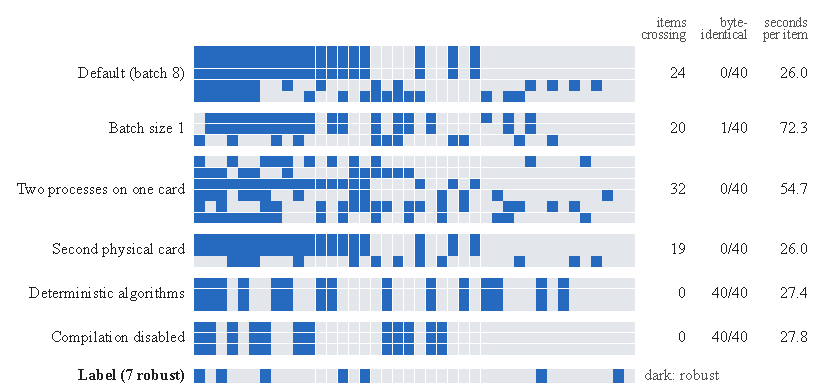
\includegraphics[width=\linewidth]{fig_rumore.pdf}
\caption{Predictions of the official pipeline for 40 preliminary public problems (columns) in 23 executions on DeepSeek (rows), by configuration; the last row is the label, dark cells are robust, and columns are sorted by how often they are predicted robust. At right: items whose prediction changes across the configuration's runs (more runs, more crossings), items whose generated text is byte-identical in all of them, and seconds per item.}
\label{fig:noise}
\end{figure}

\begin{table}[t]
\caption{Repeatability of the official pipeline on DeepSeek, 40 public problems, by configuration, in the order of Figure~\ref{fig:noise}. ``Crossings'': items whose prediction changes across the configuration's runs. ``Identical'': items whose generated text is byte-identical in all runs. Cost is runtime against the default configuration. Card 0 and card 1 are the two GPUs of the same machine. With two processes on one card, any five of its six runs give 29 to 31 crossings.}
\label{tab:reexec}
\centering
\small
\begin{tabular}{@{}lllllll@{}}
\toprule
\textbf{Configuration} & \textbf{Card} & \textbf{Runs} & \textbf{Crossings} & \textbf{Identical} & \textbf{Correct per run} & \textbf{Cost} \\
\midrule
Default (batch 8) & 0 & 5 & 24/40 & 0/40 & 24, 24, 24, 23, 24 & reference \\
Batch size 1 & 0 & 3 & 20/40 & 1/40 & 20, 21, 24 & +178\% \\
Two processes on one card & 0 & 6 & 32/40 & 0/40 & 24 to 28 & +110\% \\
Second physical card & 1 & 3 & 19/40 & 0/40 & 24, 24, 21 & +0\% \\
Deterministic algorithms & 0 & 3 & 0/40 & 40/40 & 24, 24, 24 & +5\% \\
Compilation disabled & 1 & 3 & 0/40 & 40/40 & 25, 25, 25 & +7\% \\
\bottomrule
\end{tabular}
\end{table}

\paragraph{Two candidate remedies.} Deterministic algorithms (PyTorch's, in warn-only mode, with deterministic cuDNN and a fixed cuBLAS workspace; Appendix~\ref{app:C}) and disabled compilation each made the generated text byte-identical in three sequential runs, at 5 to 7\% runtime cost. On card 0, the default configuration produced 24 crossings in five runs. Each remedy ran on one card where the default had produced crossings, each run in a new process, with no other process on that card. Three identical runs are weak evidence: the default configuration also gave three identical runs on card 0 before its fourth diverged, and five of its eight runs on the two cards shared one output. The two remedies produced different outputs, predicting 15 and 12 of the 40 problems robust, and because they ran on different cards we cannot tell whether the difference comes from the configuration or from the card. Neither gained more than one item (24 and 25 correct).

\paragraph{Distinct outputs.} The 23 executions fall into 14 distinct outputs, byte-identical within each. The same output appeared on both cards, and two runs launched in the same second on one card produced different outputs, so the output is not a property of the card alone; what selects it is not established. As only 7 of the 40 problems are robust and crossings largely cancel, accuracy moved much less than predictions: 21 to 24 correct in the default configuration on either card and 24 to 28 with two processes on one card, always below the 33 of the majority constant. An exploratory repetition of the official score extraction, whose third run ranks the 164 labeled problems at Spearman 0.24 against the first two, is in Appendix~\ref{app:C}.

\section{Regenerating the labels with our own protocol}\label{sec:labels}

\paragraph{Our labeling protocol.} We identified the organizers' perturbation families in the preliminary data (rephrase, rename, domain, distract, typos), regenerated them with gpt-oss-120b prompted with public examples, and gated each variant with gpt-oss-120b. An answer counts as correct when it matches gpt-oss-120b's answer on the original problem, because the preliminary data carry no answers; we did not check this key against the answers of the collections the problems come from. On the organizers' machine, with vLLM 0.28.0 [8] outside the official image, we labeled four models with two independent draws of variants (A and B, about 40 accepted variants per problem): 10 samples on the base problem and one per variant, at temperature 0.6, top-p 0.95 and at most 16,384 new tokens. Draw A's variants were also re-sampled with a new seed (A$'$). A label is robust when at least 6 of the 10 base samples are correct and every variant is answered correctly; unlike the earlier rule's conjunction, this requires the base problem to be solved.

A chain that reaches our cap is scored by the last boxed answer it contains, and counts as wrong without one; the organizers also count a response that reaches their limit without a parseable final answer as wrong [4]. Our protocol differs from the organizers' in perturbations, answer key, rule and sampling (one answer per variant, against 10 in the files behind most of their DeepSeek labels). Its decoding differs from the settings they publish, and its prompt may differ from the one behind their labels, which they have not stated.

\begin{table}[t]
\caption{Agreement of labels regenerated with our protocol: Cohen's kappa. The three columns for A and B treat variant chains that reached the 16,384-token cap in three ways: scored as in the protocol (by their last boxed answer, if any), dropped, or all counted as correct. The first of these columns and the A and A$'$ column give 95\% percentile bootstrap intervals over problems, and the script of Appendix~\ref{app:E} gives them for the other two. A problem has a label in a draw when it has at least one accepted variant (160 in A, 159 in B). Kappa between A and B uses the 159 problems labeled in both (150 for Qwen3.5-4B and 156 for DeepSeek when truncated chains are dropped), and between A and A$'$ 160. ``At cap'': percentage of variant chains that reached the cap in draws A and B. ``Robust'': percentage of problems labeled robust in draw A, as scored. The last column gives kappa of draw A with the organizers' preliminary DeepSeek labels: on the 138 published ones, and on the 160 that include 22 labels we derived (Section~\ref{sec:data}).}
\label{tab:label}
\centering
\small
\setlength{\tabcolsep}{3pt}
\begin{tabular}{@{}llllllll@{}}
\toprule
& & & \multicolumn{3}{l}{\textbf{A and B, truncated variant chains}} & & \\
\cmidrule(lr){4-6}
\textbf{Model} & \textbf{At cap} & \textbf{Robust} & \textbf{as scored} & \textbf{dropped} & \textbf{correct} & \textbf{A and A$'$} & \textbf{Organizers'} \\
\midrule
Skywork & 1.2, 1.5 & 74 & 0.44 [0.28, 0.59] & 0.39 & 0.39 & 0.79 [0.67, 0.89] & none \\
DeepSeek & 5.1, 6.1 & 39 & 0.41 [0.26, 0.55] & 0.35 & 0.36 & 0.46 [0.33, 0.59]$^{*}$ & 0.011; 0.025 \\
Olmo & 1.1, 0.9 & 68 & 0.38 [0.21, 0.54] & 0.39 & 0.39 & 0.65 [0.52, 0.78] & none \\
Qwen3.5-4B & 22.1, 29.2 & 9 & 0.18 [$-$0.06, 0.39] & 0.26 & 0.44 & not run & none \\
\bottomrule
\end{tabular}
\par\smallskip{\footnotesize $^{*}$On DeepSeek, A$'$ also received the answer-format line (end of this section), so this entry mixes seed and prompt.}
\end{table}

\paragraph{Results.} Under our protocol, two independent draws of variants give labels that agree at kappa 0.35 to 0.44 on Skywork, Olmo and DeepSeek, whether truncated variant chains are scored as in the protocol, dropped or all counted as correct (Table~\ref{tab:label}). On Qwen3.5-4B, 22 to 29\% of the variant chains reach the cap. Scoring these chains as in the protocol, dropping them or counting them all as correct gives agreement of 0.18, 0.26 and 0.44, and a robust share in draw A of 9\%, 83\% and 79\%. On Skywork, re-sampling the same variants with a new seed agrees far more than drawing new variants (0.79 against 0.44), so its label depends more on the variants than on the seed; on Olmo the gap is smaller (0.65 against 0.38), and on DeepSeek, where A$'$ also changed the prompt, it is 0.46 against 0.41.

Draw A's DeepSeek labels agree with the 138 labels the organizers published at kappa 0.011 [$-$0.13, 0.17], and with the 160 that include 22 of our derived labels at 0.025 [$-$0.12, 0.18]. Of the 36 problems with a published robust label, draw A calls 20 non-robust, and 4 of these change when truncated variants all count as correct. Of the 102 with a published non-robust label, draw A calls 44 robust. The reliability of the organizers' labels remains unmeasured. A retrospective calculation on the same saved answers with the main-phase threshold rule, applied as its pre-registration fixed it, with no filter on the base problem (Appendix~\ref{app:C}), gives test-retest point estimates between 0.34 and 0.56, below the pre-registered bar of 0.60, though three of the four intervals include it.

\paragraph{The prompt changes our labels.} In a first run with the bare problem text, later discarded, \mbox{Qwen3.5-4B} gave a final answer in the expected format in only 5 of its 1,640 base samples in draw A. With one instruction line requesting the format, 145 of 164 problems passed the base condition, against none. DeepSeek passed it on 147 of 164 with or without that line; its draws A and B ran without the line and A$'$ with it, and on the same variants its robust share moved from 39\% to 51\% of the 160 labeled problems, a change that mixes prompt and seed. Under our protocol, the label of Qwen3.5-4B therefore depends on the prompt. Whether this affects the organizers' labels is unknown: their baselines repository has a solve prompt that asks for an ANSWER line, but they have not said whether it was used for labeling (R3).

\section{The falsification campaign}\label{sec:campaign}

Table~\ref{tab:campaign} summarizes the campaign; Appendix~\ref{app:A} lists all 31 entries and explains three traps (rule T, the oracle H13, the duplicated pairs behind H2) and two pitfalls of the data. All entries use the preliminary data, except H16 to H18, which were scored on the 17 items of the warmup evaluation task.

\begin{table}[t]
\caption{The campaign in brief, in 19 of its 31 entries (Appendix~\ref{app:A} lists all). Ground truth is DeepSeek's and the preliminary pairs' unless stated; accuracy differences are in points against each pre-registration's baseline. H1, H7 and T count the 52 duplicated DeepSeek pairs twice; counted once, no verdict changes.}
\label{tab:campaign}
\centering
\small
\begin{tabular}{@{}L{5.5cm}L{1.9cm}L{5.6cm}@{}}
\toprule
\textbf{What we tested} & \textbf{Entries} & \textbf{Outcome} \\
\midrule
Text features; robustness as a property of the problem; labels, base accuracy and difficulty order across models & H1 to H5, H7 & rejected; H2 gained only when the duplicated pairs were counted twice \\
Official uncertainty features, logistic regression & H10 & 0.774 against a majority constant of 0.756, within the 0.692 $\pm$ 0.101 of the proposal [1] (method substituted) \\
Features cached for other models; per-target thresholds & H12, H13 & H12 rejected; the H13 ceiling withdrawn, $-$2.8 points when forced to rank \\
Our perturbation families, translation, self-consistency, the organizers' families regenerated (pilot), representation shift & H19, H22, H30 to H33 & rejected: kappa at most 0.02, AUROC at most 0.615 \\
Probes on DeepSeek's hidden states: ours and the organizers' published artifact & H36, H35 & survive their nulls; ours adds no detectable gain over length, and the artifact's score is probably in-sample \\
Trivial-robust rule, post hoc & T & a trap: +6.0 points on the preliminary pairs, +0.0 on \texttt{val-sample} \\
Identical bundles re-executed (warmup, 17 items) & H18 & noise confirmed: 11, 9, 11 and 11 correct \\
\bottomrule
\end{tabular}
\end{table}

\paragraph{Length and probes.} The character count of the problem alone orders the 164 DeepSeek labels at AUROC 0.704. Our logistic probe on DeepSeek's last-token hidden states, with layer and regularization chosen by inner cross-validation, reaches 0.710 out of fold with the original fold assignment. Over 20 other assignments, passed through the second-stage model below, it gives 0.57 to 0.76 (mean 0.69). Its scores correlate with length at Spearman +0.55, and residualized on log character count it gives 0.62. Its permutation null, rerun with 1{,}000 permutations of the whole nested procedure (the first version used 60, where 500 were pre-registered), gives $p = 0.002$. Restricted to the 138 published labels, these out-of-fold scores give 0.714 and length 0.733; retrained on those 138 alone with H36's procedure and seed, the probe gives 0.620. Combined with length in a second-stage model fitted on common outer folds, the probe changes AUROC over length alone by +0.005 on the 164 labels and by $-$0.010 on the 138 published ones (median bounds of the per-assignment 95\% intervals: $-$0.03 to 0.04, and $-$0.04 to 0.02): we detect no gain from adding the probe to length (Appendix~\ref{app:C}). This analysis replaces an earlier combination that leaked labels (Appendix~\ref{app:D}).

The organizers' published DeepSeek probe artifact orders the 164 DeepSeek labels at 0.739 with the aggregation we pre-registered and at 0.709 with its own, and at 0.62 and 0.57 residualized on log character count; its controls trained on shuffled labels give 0.68 at layer 31. The artifact does not record its training data; we infer that 137 of the 164 problems were among the public rows it was trained on, so these scores are probably largely in-sample. These length controls, which play the role of control tasks [7], were post hoc. Whether either probe reads anything beyond length that bears on robustness is not established. Apart from the three traps of Appendix~\ref{app:A}, no signal we scored by accuracy beats the majority constant by more than about one standard error on the preliminary labels, most of them DeepSeek's.

\section{Our entries}\label{sec:entries}

Our entry V8, pre-registered on 13 September, is the whole rule \texttt{return~[len(p)~>=~98 for~p~in~problems]}, with the threshold at the lower median of the 174 preliminary problems and the direction fixed on the preliminary pairs. On the original main-phase tasks it scored 11/21 and 10/19, like our entry v6 and the organizers' own entries. None of these beat the majority constant, which scores at least 11/21 and 10/19 on these tasks, and on so few items the ties do not show that length carries no signal (95\% Wilson intervals 0.32 to 0.72 and 0.32 to 0.73). On the 71 labeled rows of the official training set (revision of 17 September; 36 distinct problems), V8 differs from the all-robust constant on only 6 rows and is wrong on all 6 (46/71 against 52/71): too few to say what length is worth on official data. On the replacement tasks of 16 September, before and after the evaluation changed on 15 October [6], it predicted robust for every item (10/21 and 7/14), like an all-robust control. For the final test we nominated V8 (Codabench 1016713) and the constant (1016732), both on the Main track; our pre-registered predictions will be scored there (Appendix~\ref{app:B}).

\section{Recommendations}\label{sec:recs}

These rest mostly on DeepSeek and the preliminary data, and should be checked on the other models.
\begin{itemize}
\item \textbf{R1. Remove the variation between runs, and test the remedy:} on the same card with independent restarts, under load and across cards.
\item \textbf{R2. Repeat only where it decides something:} at the warmup's re-execution noise (a standard deviation of 1.0 item on 17, itself estimated from four runs), a one-item gap needs about eight runs per entry to reach two standard errors, so repeat only entries that run a model and sit near a prize boundary.
\item \textbf{R3. Say which prompt and decoding settings produced each released label file,} at least after the close.
\item \textbf{R4. Measure the label's reliability directly,} with two independent draws of variants labeled by the official process.
\item \textbf{R5. Show floors and noise on the leaderboard:} a row per constant predictor, the re-execution noise and binomial intervals.
\item \textbf{R6. Require a length control in white-box ablations.}
\item \textbf{R7. Remove the leaking field} \texttt{permutation\_type} from the aggregated datasets (Appendix~\ref{app:A}).
\end{itemize}

\paragraph{Code and data.} Our code, bundles, pre-registrations and outcome files are released at \href{https://github.com/Dan23RR/aimo-instrument}{\nolinkurl{github.com/Dan23RR/aimo-instrument}}. Its folder \texttt{reproduce/} recomputes the main tables from saved outputs and the six preliminary datasets, and the other numbers come from the dated records in \texttt{archive/} (Appendix~\ref{app:E}).

%%%%%% End of the main text: the six pages end here; the Limitations do not count %%%%%%
\label{fine-testo}

\section*{Limitations}

\begin{enumerate}[leftmargin=1.6em, itemsep=2pt, topsep=4pt, parsep=0pt]
\item \textbf{Preliminary data, not official data.} We did not repeat our label and probe analyses on the official training set, beyond the evaluation of V8 and a five-row check of our labels (Appendix~\ref{app:C}). Findings on label reliability and predictability may not generalize to the official evaluation setting.
\item \textbf{Our protocol, not the official one.} We did not regenerate labels with the organizers' published settings (100,000 tokens, temperature 1.0), with 10 answers per variant as in the files behind most DeepSeek labels, or on \texttt{train-main-v2}. The three treatments of truncated variant chains show how much our cap moves agreement between our draws; all three score base samples that reach the cap as the protocol does, and none of them reproduces longer decoding or a different temperature. Our low agreement with the organizers' labels is a fact about our process.
\item \textbf{One model.} We ran the probes, the re-execution study of Section~\ref{sec:reexec} and the comparisons of our regenerated labels with the organizers' preliminary labels only on DeepSeek.
\item \textbf{Re-execution.} We did not run the two candidate remedies on the same card, so card and configuration are confounded; we did not test either remedy under contention or on both cards, and we used 40 problems and one image.
\item \textbf{Records.} Some analyses rest on re-created scripts or dated records (Appendix~\ref{app:D}). Nothing here estimates performance on the final held-out problems.
\end{enumerate}

\section*{AI usage statement}

In this work, we used one generative AI tool, Claude (Anthropic), through Claude Code, for ideation, coding, analysis and writing. Ideation: it drafted the pre-registrations, including hypotheses, predictions and kill criteria, and searched and summarized the literature and the public records, including the organizers' Discord channels and the author's correspondence with them. Coding: it wrote the solution code of our bundles and the analysis and extraction scripts, ran them, and operated the organizers' virtual machine over SSH. Analysis: it computed and interpreted the results and ran automated adversarial reviews of hypotheses, drafts and code. Writing: it drafted the correspondence, this report and its revision after review.

It also made most of our Codabench uploads through the author's browser at the author's instruction. There were two exceptions: one resubmission (925822, 14 September), made without a specific instruction, and one submission that the author had not approved, sent in error and rejected before import (1016734, 28 October).

Language models were also components of our method: gpt-oss-120b generated and gated the perturbation variants and supplied the reference answers of Section~\ref{sec:labels}, and phi-4 translated problems for H22. The final decisions on the direction of the work, on the submissions (with the two exceptions above), on the nominations for the final test and on the claims of this report were the author's, and the author sent all correspondence personally. The author has reviewed all AI-assisted work and takes full responsibility for the final content of this report.

\begin{ack}
We thank Michal Štefánik, Róbert Belanec and the AIMO Interpretability team for the compute grant, a virtual machine with two GPUs, and for answering our questions; on 2 November they confirmed that the measurements taken on their machine may appear in this report. We also thank the three reviewers and the program chairs: two reviewers checked our analyses against the released code and data, and their checks corrected several of our claims. Other GPU time was rented on Modal and paid by the author or covered by Modal's platform credit. This work received no other funding, and the author has no competing interests.
\end{ack}

\section*{References}
{\small
[1] M. Štefánik, P. Mondorf, A. Waldis, Q. Liu, C. Yang, M. Spiegel, J. Kuchař, M. Kadlčík, A. Vawda-Oomerjee, C. Liu, S. Frieder, B. Plank, F. Barez and P. Stenetorp. AIMO Interpretability Challenge. CoRR, abs/2607.13899, 2026. doi:10.48550/arXiv.2607.13899.

[2] H. He and Thinking Machines Lab. Defeating Nondeterminism in LLM Inference. Thinking Machines Lab: Connectionism, 2025.

[3] J. Yuan, H. Li, X. Ding, W. Xie, Y.-J. Li, W. Zhao, K. Wan, J. Shi, X. Hu and Z. Liu. Understanding and Mitigating Numerical Sources of Nondeterminism in LLM Inference. NeurIPS 2025. arXiv:2506.09501.

[4] AIMO Interpretability Challenge website and FAQ. \url{https://aimo-interp.github.io} (accessed 28 October 2026), and its source repository aimo-interp/aimo-interp.github.io on GitHub.

[5] aimo-interp/getting-started and aimo-interp/baselines, GitHub repositories: README and issues \#6 and \#10 of getting-started; aimo-interp datasets on Hugging Face, including \texttt{train-main-v2} and \texttt{val-sample}.

[6] AIMO Interpretability Challenge Discord, \#announcements and \#qa: 5, 15 and 22 September, 9, 15, 16 and 20 October 2026.

[7] J. Hewitt and P. Liang. Designing and Interpreting Probes with Control Tasks. EMNLP-IJCNLP 2019.

[8] W. Kwon et al. Efficient Memory Management for Large Language Model Serving with PagedAttention. SOSP 2023.

[9] D. Hendrycks et al. Measuring Mathematical Problem Solving With the MATH Dataset. NeurIPS 2021 Datasets and Benchmarks Track. arXiv:2103.03874.
}

%%%%%% End of the references %%%%%%
\clearpage
\appendix
\raggedright

\input{app_A}
\input{app_B}
\input{app_C}
\input{app_D}
\input{app_E}

\newpage
\input{checklist_compilata.tex}

\end{document}
".
\usepackage[final,sglblindworkshop]{neurips_2026}
\workshoptitle{AIMO Interpretability Challenge}
\ifdefined\cleancopy\else
  \usepackage{lineno}
  \linenumbers
  \ifdefined\everyline\else\modulolinenumbers[5]\fi
  \renewcommand\linenumberfont{\normalfont\tiny\sffamily\color{black!45}}
\fi

\usepackage[utf8]{inputenc}
\usepackage[T1]{fontenc}
%% Typewriter text in Latin Modern, the Type 1 version of the default Computer Modern typewriter, with the same
%% widths: without it, \texttt in T1 encoding becomes bitmap (Type 3) fonts, and the template asks for Type 1 fonts.
\renewcommand{\ttdefault}{lmtt}
\usepackage{hyperref}
\hypersetup{pdftitle={The Instrument Behind the Leaderboard: Re-Execution Noise and Label Regeneration in the AIMO Interpretability Challenge}, pdfauthor={Daniel Culotta}}
\usepackage{url}
\def\UrlBreaks{\do\/\do\.\do\_\do\-\do\:}
\usepackage{booktabs}
\usepackage{array}
\usepackage{longtable}
\newcolumntype{L}[1]{>{\raggedright\arraybackslash}p{#1}}
\usepackage{amsfonts}
\usepackage{microtype}
\usepackage{xcolor}
\usepackage{graphicx}
\usepackage{enumitem}
\usepackage{needspace}
\setlist[itemize]{leftmargin=1.4em, itemsep=2pt, topsep=4pt, parsep=0pt}
\setlist[itemize,2]{label=$\circ$}
\renewcommand{\arraystretch}{1.15}
\raggedbottom

\title{The Instrument Behind the Leaderboard: Re-Execution Noise and Label Regeneration in the AIMO Interpretability Challenge}

\author{%
  Daniel Culotta \\
  Independent researcher
}

\begin{document}

\maketitle

\begin{abstract}
We treat the AIMO Interpretability benchmark, which asks whether a model's answer to a math problem survives perturbations, as a measurement instrument. Almost all our label and probe analyses use the preliminary datasets. As the program chairs note, these differ from the official training and validation data in sampling, perturbations and eligibility, so findings on label reliability and predictability may not hold in the official evaluation. First, on DeepSeek-R1-0528-Qwen3-8B in the official pipeline, 24 of 40 items changed prediction across five default runs. Turning compilation off, or deterministic algorithms on, gave three byte-identical runs, each on one card. Second, we regenerated labels with our own protocol, not the official one: our perturbations and answer key, one answer per variant, a 16,384-token cap and temperature 0.6, where the organizers publish 100,000 tokens and 1.0. Two independent draws agree at kappa 0.35 to 0.44 on three of four models however truncated chains are treated, and 0.18 to 0.44 on Qwen3.5-4B, whose chains often reach the cap. Draw A agrees with the 138 published DeepSeek labels at kappa 0.01. This describes our protocol and does not measure the reliability of the organizers' labels. Third, of the 27 dated hypotheses with a kill criterion, 21 failed it. Our probe on DeepSeek's hidden states does no better than problem length (AUROC 0.710 against 0.704; below length on the published labels) and adds nothing detectable to it.
\end{abstract}

\section{Introduction}\label{sec:1}

A leaderboard is a measurement. Its score is read off an instrument made of a label, an evaluation set, an inference pipeline and the hardware it runs on. When the label is itself produced by a stochastic process, the instrument has noise of its own, which a single submission cannot see. We measure the re-execution noise of the official extraction and regressor, and the repeatability of labels regenerated with our own protocol, not the noise of the organizers' labels.

We study the instrument of the AIMO Interpretability Challenge, in which a submission predicts, for a given model and math problem, whether the model's answer is robust to perturbations of the problem [1]. We ran our work as a falsification campaign: every hypothesis was recorded in a dated file, 26 of the 31 before their data were seen, and every tested hypothesis is reported. Of the 31 entries, 27 carried a kill criterion written before their test ran (for 3 of them in a written plan rather than a frozen pre-registration, and for H2 after its concordance had been seen). By that criterion 21 were rejected, 5 survived and 1 is not established (Appendix~\ref{app:A}).

\paragraph{Scope.} Three limits apply.
\begin{itemize}
\item \textbf{Preliminary and official data.} Almost all of our label and probe analyses use the six preliminary public datasets released before the main phase. Their labels follow an earlier rule than those of the official training set (\texttt{train-main-v2}) and of the validation and test tasks [5]; as the program chairs noted in their meta-review, their sampling procedures, perturbations and eligibility criteria also differ. Beyond the label rule, we did not compare the two. Unless we say otherwise, a result on labels or on their predictability holds for the preliminary data and may not hold in the official evaluation setting.
\item \textbf{Our labeling protocol is not the official one.} When we regenerate labels (Section~\ref{sec:labels}), we use our own perturbations, prompts, sampling, decoding, answer key and labeling rule. Disagreement with the organizers' preliminary labels therefore shows that the two processes give different labels; it does not establish that their labels are unreliable or irreproducible.
\item \textbf{Mostly one model.} The re-execution study of Section~\ref{sec:reexec}, the probe analyses and every comparison of our regenerated labels with the organizers' preliminary labels are on DeepSeek-R1-0528-Qwen3-8B. Regenerated labels cover four models, but no conclusion about the official benchmark is established across models.
\end{itemize}

Within these limits, Sections~\ref{sec:reexec} to~\ref{sec:campaign} report re-execution noise and two candidate remedies, our regenerated labels, and signals that do no better than problem length or come from an artifact of the data. Nondeterminism of LLM inference is documented in general [2, 3]; we add its size for one model, one submission and 40 problems on this benchmark's hardware and pipeline. We make no claim about any participant's method.

\section{The task, the labels and the data}\label{sec:data}

\paragraph{Task.} A submission receives a model identifier, a reasoning effort and a list of problems, and returns one robustness verdict per problem, offline on one GPU within one hour [4, 5], or 70 minutes since 15 October [6]. The models are Qwen3.5-4B, Skywork-OR1-Math-7B, Olmo-3-7B-Think and \mbox{DeepSeek-R1-0528-Qwen3-8B} in both tracks, and gpt-oss-120b in the Main track only.

\paragraph{Official data.} The main-phase training set \texttt{train-main-v2} labels all five models with a threshold on the largest accuracy drop across perturbation families: robust at most 0.10, non-robust at least 0.25, no label in between [5]. The organizers' published decoding settings are up to 100,000 tokens at temperature 1.0, top-k 40 and top-p 0.95, and a response that reaches the limit without a final answer counts as wrong [4]. Since 16 September the private validation tasks have 21 items (Main) and 14 (Small), on which the binomial standard error of an accuracy near one half is 10.9 and 13.4 points; the final test uses 30 to 50 new problems [5, 6].

\paragraph{Preliminary data.} Six datasets released before the main phase aggregate to 335 (model, problem) pairs over 174 distinct problems, up to eight per problem; 52 pairs repeat the DeepSeek measurements under a second model name. Their labels follow an earlier rule: on all 379 labeled rows (a pair can have several), the label equals the conjunction ``no perturbation lowered accuracy''. A per-family majority rule (``more than half of the answers are correct in every perturbation family'') reproduces the same 379 labels, so these rows cannot tell the two rules apart. Whether they used the decoding settings above is not documented; in the files behind most DeepSeek labels, most variants listed as lowering accuracy were answered 10 times. We call their labels the organizers' preliminary labels, and keep ``official'' for \texttt{train-main-v2} and the validation and test tasks.

\paragraph{DeepSeek labels.} DeepSeek is the only evaluated model with many preliminary labels: 164 distinct problems (the 52 duplicated pairs count once). For 138 of them the data publish a label. For the other 26 we derived one with the conjunction, which makes 4 of them robust; the majority rule would make 21 robust, so these 26 labels depend on the choice of rule. We therefore report results on the 138 published labels separately.

\section{Re-execution noise on the evaluation workers' type of GPU}\label{sec:reexec}

On a virtual machine lent by the organizers, with two NVIDIA RTX PRO 6000 Blackwell Server Edition GPUs (the type the evaluation workers use), we ran 40 preliminary public problems through the official runtime image, extraction and regressor, unmodified, on DeepSeek. Decoding was greedy, with at most 4,096 new tokens in batches of 8. The 40 labels are DeepSeek's of Section~\ref{sec:data}: 28 published and 12 that we derived with the conjunction, which include 3 of the 7 robust ones. Figure~\ref{fig:noise} shows the 23 executions; Table~\ref{tab:reexec} gives the repeatability of each configuration.

\begin{figure}[t]
\centering
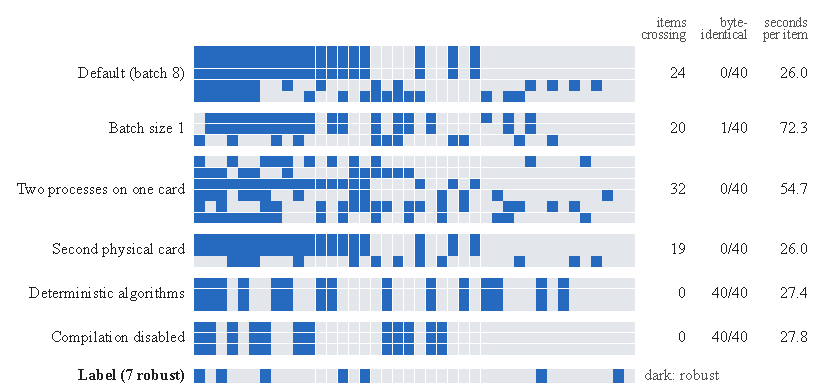
\includegraphics[width=\linewidth]{fig_rumore.pdf}
\caption{Predictions of the official pipeline for 40 preliminary public problems (columns) in 23 executions on DeepSeek (rows), by configuration; the last row is the label, dark cells are robust, and columns are sorted by how often they are predicted robust. At right: items whose prediction changes across the configuration's runs (more runs, more crossings), items whose generated text is byte-identical in all of them, and seconds per item.}
\label{fig:noise}
\end{figure}

\begin{table}[t]
\caption{Repeatability of the official pipeline on DeepSeek, 40 public problems, by configuration, in the order of Figure~\ref{fig:noise}. ``Crossings'': items whose prediction changes across the configuration's runs. ``Identical'': items whose generated text is byte-identical in all runs. Cost is runtime against the default configuration. Card 0 and card 1 are the two GPUs of the same machine. With two processes on one card, any five of its six runs give 29 to 31 crossings.}
\label{tab:reexec}
\centering
\small
\begin{tabular}{@{}lllllll@{}}
\toprule
\textbf{Configuration} & \textbf{Card} & \textbf{Runs} & \textbf{Crossings} & \textbf{Identical} & \textbf{Correct per run} & \textbf{Cost} \\
\midrule
Default (batch 8) & 0 & 5 & 24/40 & 0/40 & 24, 24, 24, 23, 24 & reference \\
Batch size 1 & 0 & 3 & 20/40 & 1/40 & 20, 21, 24 & +178\% \\
Two processes on one card & 0 & 6 & 32/40 & 0/40 & 24 to 28 & +110\% \\
Second physical card & 1 & 3 & 19/40 & 0/40 & 24, 24, 21 & +0\% \\
Deterministic algorithms & 0 & 3 & 0/40 & 40/40 & 24, 24, 24 & +5\% \\
Compilation disabled & 1 & 3 & 0/40 & 40/40 & 25, 25, 25 & +7\% \\
\bottomrule
\end{tabular}
\end{table}

\paragraph{Two candidate remedies.} Deterministic algorithms (PyTorch's, in warn-only mode, with deterministic cuDNN and a fixed cuBLAS workspace; Appendix~\ref{app:C}) and disabled compilation each made the generated text byte-identical in three sequential runs, at 5 to 7\% runtime cost. On card 0, the default configuration produced 24 crossings in five runs. Each remedy ran on one card where the default had produced crossings, each run in a new process, with no other process on that card. Three identical runs are weak evidence: the default configuration also gave three identical runs on card 0 before its fourth diverged, and five of its eight runs on the two cards shared one output. The two remedies produced different outputs, predicting 15 and 12 of the 40 problems robust, and because they ran on different cards we cannot tell whether the difference comes from the configuration or from the card. Neither gained more than one item (24 and 25 correct).

\paragraph{Distinct outputs.} The 23 executions fall into 14 distinct outputs, byte-identical within each. The same output appeared on both cards, and two runs launched in the same second on one card produced different outputs, so the output is not a property of the card alone; what selects it is not established. As only 7 of the 40 problems are robust and crossings largely cancel, accuracy moved much less than predictions: 21 to 24 correct in the default configuration on either card and 24 to 28 with two processes on one card, always below the 33 of the majority constant. An exploratory repetition of the official score extraction, whose third run ranks the 164 labeled problems at Spearman 0.24 against the first two, is in Appendix~\ref{app:C}.

\section{Regenerating the labels with our own protocol}\label{sec:labels}

\paragraph{Our labeling protocol.} We identified the organizers' perturbation families in the preliminary data (rephrase, rename, domain, distract, typos), regenerated them with gpt-oss-120b prompted with public examples, and gated each variant with gpt-oss-120b. An answer counts as correct when it matches gpt-oss-120b's answer on the original problem, because the preliminary data carry no answers; we did not check this key against the answers of the collections the problems come from. On the organizers' machine, with vLLM 0.28.0 [8] outside the official image, we labeled four models with two independent draws of variants (A and B, about 40 accepted variants per problem): 10 samples on the base problem and one per variant, at temperature 0.6, top-p 0.95 and at most 16,384 new tokens. Draw A's variants were also re-sampled with a new seed (A$'$). A label is robust when at least 6 of the 10 base samples are correct and every variant is answered correctly; unlike the earlier rule's conjunction, this requires the base problem to be solved.

A chain that reaches our cap is scored by the last boxed answer it contains, and counts as wrong without one; the organizers also count a response that reaches their limit without a parseable final answer as wrong [4]. Our protocol differs from the organizers' in perturbations, answer key, rule and sampling (one answer per variant, against 10 in the files behind most of their DeepSeek labels). Its decoding differs from the settings they publish, and its prompt may differ from the one behind their labels, which they have not stated.

\begin{table}[t]
\caption{Agreement of labels regenerated with our protocol: Cohen's kappa. The three columns for A and B treat variant chains that reached the 16,384-token cap in three ways: scored as in the protocol (by their last boxed answer, if any), dropped, or all counted as correct. The first of these columns and the A and A$'$ column give 95\% percentile bootstrap intervals over problems, and the script of Appendix~\ref{app:E} gives them for the other two. A problem has a label in a draw when it has at least one accepted variant (160 in A, 159 in B). Kappa between A and B uses the 159 problems labeled in both (150 for Qwen3.5-4B and 156 for DeepSeek when truncated chains are dropped), and between A and A$'$ 160. ``At cap'': percentage of variant chains that reached the cap in draws A and B. ``Robust'': percentage of problems labeled robust in draw A, as scored. The last column gives kappa of draw A with the organizers' preliminary DeepSeek labels: on the 138 published ones, and on the 160 that include 22 labels we derived (Section~\ref{sec:data}).}
\label{tab:label}
\centering
\small
\setlength{\tabcolsep}{3pt}
\begin{tabular}{@{}llllllll@{}}
\toprule
& & & \multicolumn{3}{l}{\textbf{A and B, truncated variant chains}} & & \\
\cmidrule(lr){4-6}
\textbf{Model} & \textbf{At cap} & \textbf{Robust} & \textbf{as scored} & \textbf{dropped} & \textbf{correct} & \textbf{A and A$'$} & \textbf{Organizers'} \\
\midrule
Skywork & 1.2, 1.5 & 74 & 0.44 [0.28, 0.59] & 0.39 & 0.39 & 0.79 [0.67, 0.89] & none \\
DeepSeek & 5.1, 6.1 & 39 & 0.41 [0.26, 0.55] & 0.35 & 0.36 & 0.46 [0.33, 0.59]$^{*}$ & 0.011; 0.025 \\
Olmo & 1.1, 0.9 & 68 & 0.38 [0.21, 0.54] & 0.39 & 0.39 & 0.65 [0.52, 0.78] & none \\
Qwen3.5-4B & 22.1, 29.2 & 9 & 0.18 [$-$0.06, 0.39] & 0.26 & 0.44 & not run & none \\
\bottomrule
\end{tabular}
\par\smallskip{\footnotesize $^{*}$On DeepSeek, A$'$ also received the answer-format line (end of this section), so this entry mixes seed and prompt.}
\end{table}

\paragraph{Results.} Under our protocol, two independent draws of variants give labels that agree at kappa 0.35 to 0.44 on Skywork, Olmo and DeepSeek, whether truncated variant chains are scored as in the protocol, dropped or all counted as correct (Table~\ref{tab:label}). On Qwen3.5-4B, 22 to 29\% of the variant chains reach the cap. Scoring these chains as in the protocol, dropping them or counting them all as correct gives agreement of 0.18, 0.26 and 0.44, and a robust share in draw A of 9\%, 83\% and 79\%. On Skywork, re-sampling the same variants with a new seed agrees far more than drawing new variants (0.79 against 0.44), so its label depends more on the variants than on the seed; on Olmo the gap is smaller (0.65 against 0.38), and on DeepSeek, where A$'$ also changed the prompt, it is 0.46 against 0.41.

Draw A's DeepSeek labels agree with the 138 labels the organizers published at kappa 0.011 [$-$0.13, 0.17], and with the 160 that include 22 of our derived labels at 0.025 [$-$0.12, 0.18]. Of the 36 problems with a published robust label, draw A calls 20 non-robust, and 4 of these change when truncated variants all count as correct. Of the 102 with a published non-robust label, draw A calls 44 robust. The reliability of the organizers' labels remains unmeasured. A retrospective calculation on the same saved answers with the main-phase threshold rule, applied as its pre-registration fixed it, with no filter on the base problem (Appendix~\ref{app:C}), gives test-retest point estimates between 0.34 and 0.56, below the pre-registered bar of 0.60, though three of the four intervals include it.

\paragraph{The prompt changes our labels.} In a first run with the bare problem text, later discarded, \mbox{Qwen3.5-4B} gave a final answer in the expected format in only 5 of its 1,640 base samples in draw A. With one instruction line requesting the format, 145 of 164 problems passed the base condition, against none. DeepSeek passed it on 147 of 164 with or without that line; its draws A and B ran without the line and A$'$ with it, and on the same variants its robust share moved from 39\% to 51\% of the 160 labeled problems, a change that mixes prompt and seed. Under our protocol, the label of Qwen3.5-4B therefore depends on the prompt. Whether this affects the organizers' labels is unknown: their baselines repository has a solve prompt that asks for an ANSWER line, but they have not said whether it was used for labeling (R3).

\section{The falsification campaign}\label{sec:campaign}

Table~\ref{tab:campaign} summarizes the campaign; Appendix~\ref{app:A} lists all 31 entries and explains three traps (rule T, the oracle H13, the duplicated pairs behind H2) and two pitfalls of the data. All entries use the preliminary data, except H16 to H18, which were scored on the 17 items of the warmup evaluation task.

\begin{table}[t]
\caption{The campaign in brief, in 19 of its 31 entries (Appendix~\ref{app:A} lists all). Ground truth is DeepSeek's and the preliminary pairs' unless stated; accuracy differences are in points against each pre-registration's baseline. H1, H7 and T count the 52 duplicated DeepSeek pairs twice; counted once, no verdict changes.}
\label{tab:campaign}
\centering
\small
\begin{tabular}{@{}L{5.5cm}L{1.9cm}L{5.6cm}@{}}
\toprule
\textbf{What we tested} & \textbf{Entries} & \textbf{Outcome} \\
\midrule
Text features; robustness as a property of the problem; labels, base accuracy and difficulty order across models & H1 to H5, H7 & rejected; H2 gained only when the duplicated pairs were counted twice \\
Official uncertainty features, logistic regression & H10 & 0.774 against a majority constant of 0.756, within the 0.692 $\pm$ 0.101 of the proposal [1] (method substituted) \\
Features cached for other models; per-target thresholds & H12, H13 & H12 rejected; the H13 ceiling withdrawn, $-$2.8 points when forced to rank \\
Our perturbation families, translation, self-consistency, the organizers' families regenerated (pilot), representation shift & H19, H22, H30 to H33 & rejected: kappa at most 0.02, AUROC at most 0.615 \\
Probes on DeepSeek's hidden states: ours and the organizers' published artifact & H36, H35 & survive their nulls; ours adds no detectable gain over length, and the artifact's score is probably in-sample \\
Trivial-robust rule, post hoc & T & a trap: +6.0 points on the preliminary pairs, +0.0 on \texttt{val-sample} \\
Identical bundles re-executed (warmup, 17 items) & H18 & noise confirmed: 11, 9, 11 and 11 correct \\
\bottomrule
\end{tabular}
\end{table}

\paragraph{Length and probes.} The character count of the problem alone orders the 164 DeepSeek labels at AUROC 0.704. Our logistic probe on DeepSeek's last-token hidden states, with layer and regularization chosen by inner cross-validation, reaches 0.710 out of fold with the original fold assignment. Over 20 other assignments, passed through the second-stage model below, it gives 0.57 to 0.76 (mean 0.69). Its scores correlate with length at Spearman +0.55, and residualized on log character count it gives 0.62. Its permutation null, rerun with 1{,}000 permutations of the whole nested procedure (the first version used 60, where 500 were pre-registered), gives $p = 0.002$. Restricted to the 138 published labels, these out-of-fold scores give 0.714 and length 0.733; retrained on those 138 alone with H36's procedure and seed, the probe gives 0.620. Combined with length in a second-stage model fitted on common outer folds, the probe changes AUROC over length alone by +0.005 on the 164 labels and by $-$0.010 on the 138 published ones (median bounds of the per-assignment 95\% intervals: $-$0.03 to 0.04, and $-$0.04 to 0.02): we detect no gain from adding the probe to length (Appendix~\ref{app:C}). This analysis replaces an earlier combination that leaked labels (Appendix~\ref{app:D}).

The organizers' published DeepSeek probe artifact orders the 164 DeepSeek labels at 0.739 with the aggregation we pre-registered and at 0.709 with its own, and at 0.62 and 0.57 residualized on log character count; its controls trained on shuffled labels give 0.68 at layer 31. The artifact does not record its training data; we infer that 137 of the 164 problems were among the public rows it was trained on, so these scores are probably largely in-sample. These length controls, which play the role of control tasks [7], were post hoc. Whether either probe reads anything beyond length that bears on robustness is not established. Apart from the three traps of Appendix~\ref{app:A}, no signal we scored by accuracy beats the majority constant by more than about one standard error on the preliminary labels, most of them DeepSeek's.

\section{Our entries}\label{sec:entries}

Our entry V8, pre-registered on 13 September, is the whole rule \texttt{return~[len(p)~>=~98 for~p~in~problems]}, with the threshold at the lower median of the 174 preliminary problems and the direction fixed on the preliminary pairs. On the original main-phase tasks it scored 11/21 and 10/19, like our entry v6 and the organizers' own entries. None of these beat the majority constant, which scores at least 11/21 and 10/19 on these tasks, and on so few items the ties do not show that length carries no signal (95\% Wilson intervals 0.32 to 0.72 and 0.32 to 0.73). On the 71 labeled rows of the official training set (revision of 17 September; 36 distinct problems), V8 differs from the all-robust constant on only 6 rows and is wrong on all 6 (46/71 against 52/71): too few to say what length is worth on official data. On the replacement tasks of 16 September, before and after the evaluation changed on 15 October [6], it predicted robust for every item (10/21 and 7/14), like an all-robust control. For the final test we nominated V8 (Codabench 1016713) and the constant (1016732), both on the Main track; our pre-registered predictions will be scored there (Appendix~\ref{app:B}).

\section{Recommendations}\label{sec:recs}

These rest mostly on DeepSeek and the preliminary data, and should be checked on the other models.
\begin{itemize}
\item \textbf{R1. Remove the variation between runs, and test the remedy:} on the same card with independent restarts, under load and across cards.
\item \textbf{R2. Repeat only where it decides something:} at the warmup's re-execution noise (a standard deviation of 1.0 item on 17, itself estimated from four runs), a one-item gap needs about eight runs per entry to reach two standard errors, so repeat only entries that run a model and sit near a prize boundary.
\item \textbf{R3. Say which prompt and decoding settings produced each released label file,} at least after the close.
\item \textbf{R4. Measure the label's reliability directly,} with two independent draws of variants labeled by the official process.
\item \textbf{R5. Show floors and noise on the leaderboard:} a row per constant predictor, the re-execution noise and binomial intervals.
\item \textbf{R6. Require a length control in white-box ablations.}
\item \textbf{R7. Remove the leaking field} \texttt{permutation\_type} from the aggregated datasets (Appendix~\ref{app:A}).
\end{itemize}

\paragraph{Code and data.} Our code, bundles, pre-registrations and outcome files are released at \href{https://github.com/Dan23RR/aimo-instrument}{\nolinkurl{github.com/Dan23RR/aimo-instrument}}. Its folder \texttt{reproduce/} recomputes the main tables from saved outputs and the six preliminary datasets, and the other numbers come from the dated records in \texttt{archive/} (Appendix~\ref{app:E}).

%%%%%% End of the main text: the six pages end here; the Limitations do not count %%%%%%
\label{fine-testo}

\section*{Limitations}

\begin{enumerate}[leftmargin=1.6em, itemsep=2pt, topsep=4pt, parsep=0pt]
\item \textbf{Preliminary data, not official data.} We did not repeat our label and probe analyses on the official training set, beyond the evaluation of V8 and a five-row check of our labels (Appendix~\ref{app:C}). Findings on label reliability and predictability may not generalize to the official evaluation setting.
\item \textbf{Our protocol, not the official one.} We did not regenerate labels with the organizers' published settings (100,000 tokens, temperature 1.0), with 10 answers per variant as in the files behind most DeepSeek labels, or on \texttt{train-main-v2}. The three treatments of truncated variant chains show how much our cap moves agreement between our draws; all three score base samples that reach the cap as the protocol does, and none of them reproduces longer decoding or a different temperature. Our low agreement with the organizers' labels is a fact about our process.
\item \textbf{One model.} We ran the probes, the re-execution study of Section~\ref{sec:reexec} and the comparisons of our regenerated labels with the organizers' preliminary labels only on DeepSeek.
\item \textbf{Re-execution.} We did not run the two candidate remedies on the same card, so card and configuration are confounded; we did not test either remedy under contention or on both cards, and we used 40 problems and one image.
\item \textbf{Records.} Some analyses rest on re-created scripts or dated records (Appendix~\ref{app:D}). Nothing here estimates performance on the final held-out problems.
\end{enumerate}

\section*{AI usage statement}

In this work, we used one generative AI tool, Claude (Anthropic), through Claude Code, for ideation, coding, analysis and writing. Ideation: it drafted the pre-registrations, including hypotheses, predictions and kill criteria, and searched and summarized the literature and the public records, including the organizers' Discord channels and the author's correspondence with them. Coding: it wrote the solution code of our bundles and the analysis and extraction scripts, ran them, and operated the organizers' virtual machine over SSH. Analysis: it computed and interpreted the results and ran automated adversarial reviews of hypotheses, drafts and code. Writing: it drafted the correspondence, this report and its revision after review.

It also made most of our Codabench uploads through the author's browser at the author's instruction. There were two exceptions: one resubmission (925822, 14 September), made without a specific instruction, and one submission that the author had not approved, sent in error and rejected before import (1016734, 28 October).

Language models were also components of our method: gpt-oss-120b generated and gated the perturbation variants and supplied the reference answers of Section~\ref{sec:labels}, and phi-4 translated problems for H22. The final decisions on the direction of the work, on the submissions (with the two exceptions above), on the nominations for the final test and on the claims of this report were the author's, and the author sent all correspondence personally. The author has reviewed all AI-assisted work and takes full responsibility for the final content of this report.

\begin{ack}
We thank Michal Štefánik, Róbert Belanec and the AIMO Interpretability team for the compute grant, a virtual machine with two GPUs, and for answering our questions; on 2 November they confirmed that the measurements taken on their machine may appear in this report. We also thank the three reviewers and the program chairs: two reviewers checked our analyses against the released code and data, and their checks corrected several of our claims. Other GPU time was rented on Modal and paid by the author or covered by Modal's platform credit. This work received no other funding, and the author has no competing interests.
\end{ack}

\section*{References}
{\small
[1] M. Štefánik, P. Mondorf, A. Waldis, Q. Liu, C. Yang, M. Spiegel, J. Kuchař, M. Kadlčík, A. Vawda-Oomerjee, C. Liu, S. Frieder, B. Plank, F. Barez and P. Stenetorp. AIMO Interpretability Challenge. CoRR, abs/2607.13899, 2026. doi:10.48550/arXiv.2607.13899.

[2] H. He and Thinking Machines Lab. Defeating Nondeterminism in LLM Inference. Thinking Machines Lab: Connectionism, 2025.

[3] J. Yuan, H. Li, X. Ding, W. Xie, Y.-J. Li, W. Zhao, K. Wan, J. Shi, X. Hu and Z. Liu. Understanding and Mitigating Numerical Sources of Nondeterminism in LLM Inference. NeurIPS 2025. arXiv:2506.09501.

[4] AIMO Interpretability Challenge website and FAQ. \url{https://aimo-interp.github.io} (accessed 28 October 2026), and its source repository aimo-interp/aimo-interp.github.io on GitHub.

[5] aimo-interp/getting-started and aimo-interp/baselines, GitHub repositories: README and issues \#6 and \#10 of getting-started; aimo-interp datasets on Hugging Face, including \texttt{train-main-v2} and \texttt{val-sample}.

[6] AIMO Interpretability Challenge Discord, \#announcements and \#qa: 5, 15 and 22 September, 9, 15, 16 and 20 October 2026.

[7] J. Hewitt and P. Liang. Designing and Interpreting Probes with Control Tasks. EMNLP-IJCNLP 2019.

[8] W. Kwon et al. Efficient Memory Management for Large Language Model Serving with PagedAttention. SOSP 2023.

[9] D. Hendrycks et al. Measuring Mathematical Problem Solving With the MATH Dataset. NeurIPS 2021 Datasets and Benchmarks Track. arXiv:2103.03874.
}

%%%%%% End of the references %%%%%%
\clearpage
\appendix
\raggedright

\section{The hypotheses, three traps and two pitfalls of the preliminary data}\label{app:A}

Section~\ref{sec:campaign} summarizes these entries. Unless stated, the ground truth is the 335 public pairs for H1 to H9 and T, the other models' preliminary labels for H12 to H15, the 17 items of the warmup evaluation set for H16 to H18, and DeepSeek's labels for the others. Validation that fits on some problems and tests on others is grouped by problem. The cross-model tests H7 and H12 to H15 hold out the model but not the problem, so part of them is in-sample; H7, H12, H14 and H15 were rejected anyway, and H13 is withdrawn. Numbers are accuracy points against each pre-registration's baseline unless they are kappa or AUROC.

{\small\setlength{\tabcolsep}{4pt}\renewcommand{\arraystretch}{1.2}
\begin{longtable}{L{1.1cm}L{3.9cm}L{5.6cm}L{2.0cm}}
\toprule
\textbf{ID} & \textbf{Hypothesis} & \textbf{Result} & \textbf{Verdict} \\
\midrule
\endfirsthead
\toprule
\textbf{ID} & \textbf{Hypothesis} & \textbf{Result} & \textbf{Verdict} \\
\midrule
\endhead
\bottomrule
\endlastfoot
H1 & The problem text predicts robustness (32 features) & 0.675 against 0.761, $-$8.7 ($-$7.4 with the duplicated pairs counted once) & rejected \\
H2 & Robustness is a property of the problem & with the 52 duplicated pairs counted once, z~=~0.88 and $-$1.3 against the per-model majority (bar 4.0); z~=~4.04 and +3.4 only when they are counted twice & rejected \\
H3 & One model's label predicts another's & $-$7.3 & rejected \\
H4 & One model's base accuracy predicts another's robustness & $-$11.8 & rejected \\
H5 & The difficulty order transfers across models & $-$25.4 & rejected \\
H6 & The same, with the oracle number of positives & $-$13.0 & ceiling (no kill criterion) \\
H7 & Base accuracy beats the prior on held-out models & $-$1.2 against the per-model majority that its pre-registration named (+0.0 against the global prior we used instead) & rejected \\
T & Robust if and only if base accuracy is below 0.05 (post hoc; see the traps below) & +6.0 on the 335 public pairs, +0.0 on \texttt{val-sample} & trap (no kill criterion) \\
H10 & The official uncertainty features reach the accuracy the proposal reports & 0.774 against a majority constant of 0.756, within 0.692 $\pm$ 0.101 [1]; a logistic regression on 13 of the 14 features of our own A100 re-implementation of the extraction (three of them constant), substituted for the official regressor & confirmed (method substituted, not declared at the time) \\
H11b & Length, saturation and trend features add signal & $-$1.8 and $-$2.5 & rejected \\
H12 & A cached model's uncertainty features predict other models & $-$16.5 & rejected \\
H13 & The same, with a threshold chosen per target & +7.3, from thresholds chosen on the scored items; $-$2.8 when forced to rank & withdrawn (no kill criterion) \\
H14, H15 & Calibration by the target's rate or by the global rate & $-$2.8 and $-$10.1 & rejected \\
H16 & Every model measured by itself beats the constant & 10/17 against 9/17 on one execution, inside the noise of H18 & survives, within noise \\
H17 & A gpt-oss threshold calibrated on \texttt{val-sample} beats H16 & 11/17, then 9, 11 and 11 on re-execution; 9/17 meets the kill criterion & not established \\
H18 & Identical bundles score differently across executions & 11, 9, 11 and 11 correct & confirmed (no kill criterion) \\
H19 & Our five mechanical perturbation families reproduce the organizers' preliminary label & accuracy 0.354 against 0.788, kappa 0.02 & rejected \\
H20 & A threshold tuned on our label transfers & 0.212 against 0.788 & rejected \\
H22 & Stability under translation reproduces the organizers' preliminary label & 0.507 against 0.740, kappa $-$0.10 & rejected \\
H23 & A threshold tuned on it transfers & +0.0 & rejected \\
H29 & Representation-distance features are repeatable (gate; written plan, not a frozen pre-registration) & ICC 0.997 to 0.999, from the dated outcome file & passes \\
H30 & The representation shift under perturbation predicts the label (written plan) & AUROC 0.615, below the kill threshold of 0.655; character count 0.704 (0.705 in E11's own computation) & rejected \\
H31 & The direction of that shift predicts the label (written plan) & AUROC 0.555 & rejected \\
H32 & The organizers' families, regenerated (pilot), reproduce their label & kappa $-$0.001 on four families, $-$0.030 with all five & rejected \\
H33 & Self-consistency over 8 samples predicts the label & AUROC 0.502 & rejected \\
H35 & The organizers' published probe artifact orders the 164 DeepSeek labels & 0.739 under the pre-registered aggregation and 0.709 under its own; 0.62 and 0.57 once residualized on log character count; its shuffled-label controls give 0.68 at layer 31 & survives its null; probably in-sample, not separated from length \\
H36 & Our linear probe, nested cross-validation, orders the 164 DeepSeek labels & 0.710 out of fold, above its permutation null, and 0.62 once residualized on log character count; 0.714 against 0.733 for length on the 138 published labels (Appendix~\ref{app:C}) & survives its null; no detectable gain over length \\
E13b-1 & Under the main-phase rule our regenerated label is test-retest reliable (kappa at least 0.60 on 3 of 4 models) & 0.34 to 0.56, retrospective (Appendix~\ref{app:C}) & rejected \\
E13b-2 & Under the main-phase rule it agrees with DeepSeek labels we computed with that rule from the preliminary data (kappa at least 0.40) & 0.02 [$-$0.09, 0.13] & rejected \\
E13b-3 & The labeling rule drives the instability of our regenerated labels & a gain of at least 0.15 on 2 of 4 models, where 3 were required; 0 of 4 on common problems & rejected \\
\end{longtable}
}

Not in the table are H8, H9, H21, H24 and H25 to H28. H8 is an oracle ceiling: 0.774, +1.8 points against the global constant and +0.4 against the per-model majority, with the duplicated pairs counted once. The outcome of H9 became rule T. H21 and H24 needed H19 and H20, and H22 and H23, to survive, so they were not run. H25 to H28 are entries of the E11 plan that its outcome file does not report under these identifiers. H25 is an anomaly of our own re-implementation of the extraction, found before the plan. H26 is the list field of the first pitfall below. H27 is a label-noise ceiling, which the plan itself closed with a resampling estimate instead of a test. H28 is the text-only baseline, which became character count (Appendix~\ref{app:D}). Three further E11 tests were not run (Appendix~\ref{app:D}). V4, an entry submitted once against its own pre-registered rule, is in Appendix~\ref{app:D}.

\paragraph{Three traps.} Rule T gains six points on the public pairs and nothing on \texttt{val-sample}, because the trivially robust items (base accuracy 0, robust under the conjunction) are absent there. The oracle H13 chose each target's threshold among all cut points on the very items it was scored on; forced to rank the items and to predict the true number of positives, it gave $-$2.8. H2 owed its survival to one measurement published under two model names and counted twice; counted once, its z falls from 4.04 to 0.88.

\paragraph{Two pitfalls of the preliminary data.} In the three aggregated datasets, the field \texttt{permutation\_type} is a list if and only if the item is robust, because the aggregation merges all perturbation types into one row for robust items and keeps one row per retained type otherwise, usually a single type. The rule ``robust if the field is a list'' reproduces all 223 labeled rows of the three datasets, and the field does not exist at inference (recommendation R7). And 20 of the 80 robust pairs among the 335 have base accuracy 0. None of them carries a published label, so they are robust only under the conjunction we used to derive their labels, while \texttt{val-sample} has no labeled pair with base accuracy below 0.05.

\section{Pre-registered predictions for the final evaluation}\label{app:B}

P1 was written on 7 September 2026, P-V8 on 13 September and P-V8b on 21 September. They are translated from the dated files and shortened. We omit the runtime predictions (under 60 seconds), which we could not score because the bundles log no runtime. A second prediction written with P1 on 7 September concerns another participant's final score and is not reported here.

\begin{itemize}
\item \textbf{P1.} The top-ranked entry's accuracy on the final held-out problems will lie within two binomial standard errors of that set's majority-class constant.
\item \textbf{P-V8.} If the organizers had neutralized length, V8 would score between 0.45 and 0.55 on both tracks (stated beforehand as the most likely outcome); if they had not, and the set was balanced, about 0.66. Observed on the original tasks: 0.52 and 0.53, inside the first band; on 21 and 19 items, however, 0.66 lies inside the 95\% intervals of both scores, so the scores do not exclude the second.
\item \textbf{P-V8b}, on the replacement tasks: the same bundles work with the new ingestion and score 6 to 15 of 21 and 4 to 10 of 14. Observed: coverage 1.0, no invalid predictions, 10/21 and 7/14, inside the bands but degenerately, since the rule predicted robust for every item.
\end{itemize}

\section{Protocols, run manifest and recalculations}\label{app:C}

\paragraph{Hardware and software.} The generation runs used the organizers' virtual machine with two NVIDIA RTX PRO 6000 Blackwell Server Edition GPUs (96 GB each), the evaluation workers' model, from 8 September 2026. Each run used one GPU; the Olmo-3-7B-Think A$'$ labels combine two runs, one on each card (below).
\begin{itemize}
\item \textbf{Official runtime image.} Section~\ref{sec:reexec} and the official score channel (E16) ran inside it: {\footnotesize\path{ghcr.io/aimo-interp/aimo-codabench-runtime:torch2.12.1-cuda13.2-cudnn9-transformers5.13.0-sklearn1.8.0-kernels0.15.2}}, digest {\footnotesize\path{sha256:fb4dab6343de7ce022ddd7906493f9ced16ff9008d497326a781d1e5adc8207a}}. They used the official extraction and regressor as shipped in our bundles: greedy decoding, at most 4,096 new tokens, static cache, batch 8.
\item \textbf{Labeling environment.} Section~\ref{sec:labels} ran with vLLM 0.28.0, torch 2.13.0 and transformers 5.16.1 (driver 610.57.04 with CUDA 13.3 on the machine, CUDA 13.0 runtime libraries in the environment) in a separate environment on the same machine; \texttt{vm\_backup/AMBIENTE\_VM\_2026-09-17.txt} lists every package.
\item \textbf{Model revisions.} Hugging Face snapshot hashes: Qwen3.5-4B \texttt{851bf6e8}, Skywork-OR1-Math-7B \texttt{fcef970f}, Olmo-3-7B-Think \texttt{d97e442d}, DeepSeek-R1-0528-Qwen3-8B \texttt{6e8885a6}, gpt-oss-120b \texttt{b5c939de}. The full hashes are in the run logs.
\item \textbf{Analyses.} They ran on CPU: E13's analysis and E15's evaluation, up to 14 September, on the virtual machine (Python 3.12, NumPy 2.3.5, scikit-learn 1.9.1), the others on the author's computer (Python 3.11.12, NumPy 2.4.4 and scikit-learn 1.8.0, as recorded for the runs of September and November). The release pins every output by SHA-256 in \texttt{MANIFEST.tsv}.
\end{itemize}

\needspace{8\baselineskip}
\paragraph{Run manifest.}
\begin{itemize}
\item \textbf{Where they ran.} The scripts in \texttt{vm/} written up to 14 September (setup, generation, extraction, E13's analysis and E15's evaluation), after which the machine stayed idle, and the clean-up script of 17 September ran on the virtual machine; the later ones ran on the author's computer.
\item \textbf{Outputs} are in \texttt{vm\_risultati/} unless the table gives another path.
\item \textbf{GPU-hours} are times from the logs (\texttt{reproduce/compute\_hours.py}). They include model loading except for the E13 labels, a difference under 1\%.
\end{itemize}

{\small\setlength{\tabcolsep}{4pt}
\begin{longtable}{L{2.4cm}L{3.2cm}L{2.2cm}>{\raggedright\arraybackslash\footnotesize}p{4.8cm}}
\toprule
\textbf{Run} & \textbf{Where it ran} & \textbf{GPU-hours} & \textbf{Outputs} \\
\midrule
\endfirsthead
\toprule
\textbf{Run} & \textbf{Where it ran} & \textbf{GPU-hours} & \textbf{Outputs} \\
\midrule
\endhead
\bottomrule
\endlastfoot
E13 variants & virtual machine & 1.15 and 1.20 & \path{e13/varianti_D1.parquet}, \path{e13/varianti_D2.parquet} \\
E13 labels & virtual machine, one queue per card & 64.4, in the logs of the 11 runs of Table~\ref{tab:label} & \path{e13/etich_*.parquet} \\
E13b, main-phase rule & author's computer & CPU only & \path{e13b_regola_nuova_2026-09-21.txt} \\
E14 re-execution & virtual machine, official image & 8.4 & \path{e14/out/*.jsonl}, \path{e14/log/} \\
E15 extraction & virtual machine & under 0.1 & \path{vm_backup/estratto/work/aimo/e15/hs_*.npz} \\
E15 probes & the virtual machine's CPU on 14 September, then the author's computer & CPU only & \path{e15_*}, \path{e15r/}, \path{vm_backup/estratto/work/aimo/e15_valuta.log} \\
E16 score channel & virtual machine, official image & 5.9 & \path{e16_*.jsonl}, \path{e16nodet/} \\
\end{longtable}
}

\paragraph{Commands.} Script paths are relative to \texttt{archive/}, the working folder of the repository. The scripts in \texttt{vm/} that ran on the virtual machine use paths under \texttt{/work/aimo}. \texttt{M} stands for the model, and in E14 \texttt{C}, \texttt{r}, \texttt{g} and \texttt{t} for the configuration, repetition, card and process tag.
\begin{itemize}
\item \textbf{E13 variants.} \texttt{vm/e13\_varianti.py -{}-draw~D1 -{}-seed~20260913 -{}-n~164 -{}-k~10}, and \texttt{-{}-draw~D2 -{}-seed~20260914}. The model gpt-oss-120b generates, solves and gates the variants (prompts below).
\item \textbf{E13 labels.} DeepSeek A and B ran an earlier version of \texttt{e13\_etichetta.py} that sent the bare problem text (now \texttt{-{}-prompt~nudo}); every other run behind Table~\ref{tab:label}, DeepSeek A$'$ included, used the explicit prompt. Draw A: \texttt{vm/e13\_etichetta.py -{}-model~M -{}-cond~A -{}-draw~D1 -{}-seed~20260921 -{}-prompt~esplicito}; B: \texttt{-{}-cond~B -{}-draw~D2 -{}-seed~20260922}; A$'$: \texttt{-{}-cond~Ap -{}-draw~D1 -{}-seed~20260923}. \texttt{vm/e13\_coda.sh} launched one queue per card (its logs are in \path{vm_backup/estratto/work/aimo/}); the card 0 queue ran an earlier version that passed no \texttt{-{}-prompt} flag, so DeepSeek A$'$ got the default of \texttt{e13\_etichetta.py}, the explicit prompt.
\item \textbf{E13b.} \texttt{vm/e13b\_regola\_nuova.py}, on the saved E13 answers; retrospective (below).
\item \textbf{E14.} \texttt{vm/e14\_all.sh 40 "C0 C1 C2 C3"} and \texttt{vm/e14\_extra.sh 1 "C5 C4"}. Each run is \texttt{e14\_run.py -{}-cond~C -{}-rep~r -{}-gpu~g -{}-tag~t -{}-n~40} inside the official image: 23 runs on DeepSeek. In the 8.4 GPU-hours the two processes of each contention pair, which shared one GPU, count once (20 runs).
\item \textbf{E15 extraction.} \texttt{vm/e15\_estrai.py -{}-model~deepseek-ai/DeepSeek-R1-0528-Qwen3-8B}, with and without the official system prompt: one forward pass per problem, last input token, all 37 hidden-state indices, at most 2,048 tokens.
\item \textbf{E15 probes.} \texttt{vm/e15\_valuta.py} ran H35, H36 and the first null (60 permutations) on 14 September, on the virtual machine's CPU; its log is \path{vm_backup/estratto/work/aimo/e15_valuta.log}. The file \path{vm_risultati/e15_valuta_2026-09-14.txt} is a later run of that day, by the file times in \path{vm_backup/MANIFEST_backup_aimo_2026-09-17.txt}, that stopped with an error at the null. H35's null is the 95th percentile, 0.602, of the AUROC of 20{,}000 random scores on the same labels, in either orientation. \texttt{vm/e15\_null\_nidificato.py} reran that null on 23 September with both grids of $C$, on the author's computer. E15-R (below) is \texttt{vm/e15r\_ricalcolo.py}, given an output folder and a number of worker processes (5 on the author's computer, 14.5 hours); its outputs are in \texttt{vm\_risultati/e15r}, and since it appends to existing files, a rerun needs a new folder. H35 needs the organizers' artifact \texttt{probe\_artifact.pkl} (hash below), which we do not redistribute.
\item \textbf{E16.} \texttt{vm/e16\_all.sh} and \texttt{vm/e16\_nodet.sh}, in the official image. Of the variables that \texttt{e16\_all.sh} sets, only the cuBLAS workspace variable reaches the extraction; \texttt{e16\_nodet.sh} sets neither.
\end{itemize}

The organizers' artifact used by H35 has SHA-256 {\footnotesize\texttt{8607478c7408922a6490adb7bda34d6a7d95403b7aa62f80dd3f2649139ccdeb}}. The listed logs total 82.8 GPU-hours. Not in the table:
\begin{itemize}
\item two complete runs of Qwen3.5-4B with the bare prompt (about 13 GPU-hours, no released log);
\item a partial run of Qwen3.5-4B A$'$ with the bare prompt (1.7 GPU-hours, included in the 82.8), discarded with them;
\item a run of Olmo-3-7B-Think A$'$ on card 1 (11.0 GPU-hours, 07:19 to 18:21 UTC on 10 September, from its queue log). Card 0 reached the same condition at 14:20, resumed from its partial file with 96 of the 164 problems done and finished the other 68, so the reported A$'$ labels come from both cards.
\end{itemize}
With these, the virtual machine ran about 107 GPU-hours, plus short smoke and feasibility tests. Our earlier runs on Modal used about 12 to 13 GPU-hours, mostly on A100 GPUs, as documented in their dated outcome files: the feature extraction behind H10, its pilot, and E9 to E12.

\paragraph{What can be recomputed.}
\begin{itemize}
\item \textbf{From saved outputs.} The scripts in \texttt{reproduce/} (Appendix~\ref{app:E}), which also read the six preliminary datasets; the other numbers come from the dated records in \texttt{archive/}.
\item \textbf{On a CPU, from the released hidden states.} Our probe (H36) and E15-R can be rerun end to end. H35 also needs the organizers' artifact.
\item \textbf{Only with the original GPUs and models.} The generation runs.
\end{itemize}

\paragraph{Re-execution configurations (Section~\ref{sec:reexec}).}
\begin{itemize}
\item \textbf{C0, default:} batch 8, on card 0, five runs.
\item \textbf{C1, batch size 1.}
\item \textbf{C2, deterministic algorithms:} \texttt{torch.use\_deterministic\_algorithms(True, warn\_only=True)}, \texttt{cudnn.deterministic = True}, \texttt{cudnn.benchmark = False} and \texttt{CUBLAS\_WORKSPACE\_CONFIG=:4096:8}.
\item \textbf{C3, contention:} two identical processes at the same time on card 0, three pairs.
\item \textbf{C4, second card:} the default on card 1.
\item \textbf{C5, compilation disabled:} \texttt{TORCH\_COMPILE\_DISABLE=1}, on card 1.
\end{itemize}
Runs within a configuration were sequential, each a new process. During these runs the other card was running another of our jobs. Two pre-registered predictions failed:
\begin{itemize}
\item batch size 1 did not make generation more repeatable: three runs gave three different outputs;
\item disabled compilation was predicted to land in one of the default outputs; it was byte-identical across its runs, but in an output of its own.
\end{itemize}
\texttt{reproduce/reexecution\_table.py} recomputes Table~\ref{tab:reexec} and the numbers of Figure~\ref{fig:noise}, and lists the 14 distinct outputs.

\paragraph{Variants and labels (Section~\ref{sec:labels}).}
\begin{itemize}
\item \textbf{Few-shot pool.} The generator saw five public examples of each family, drawn from a pool of 621 public examples (original, perturbed) over the five families. The texts are the organizers' and are not redistributed. \texttt{vm\_risultati/e13/fewshot\_pool\_ids.json} lists each example's problem identifier and SHA-256 hashes, and \texttt{reproduce/fewshot\_pool.py} rebuilds the pool from the downloaded preliminary datasets (verified on 23 November 2026: 621 of 621, byte-identical).
\item \textbf{Drawing the examples.} For draw seed $s$, problem $p$ and family $f$, the five examples are \texttt{random.Random("s|p|f").sample(pool[f] without p, 5)}.
\item \textbf{Generator.} gpt-oss-120b at low reasoning effort, temperature 1.0, top-p 1.0, at most 4,096 tokens, one request per problem and family, asking for 10 variants.
\item \textbf{Gate and reference answers.} gpt-oss-120b at medium effort, temperature 1.0, at most 8,192 tokens, solves the original and each variant. A variant is accepted if its text differs from the original, the length ratio lies between 0.7 and 4.0, and the solver's answer is unchanged. The solver's answer on the original is the reference answer.
\item \textbf{Labeling.}
  \begin{itemize}
  \item \textbf{Prompt.} Each model receives the instruction line (the second block below) followed by the problem, except DeepSeek in A and B, which received the bare text.
  \item \textbf{Sampling.} Temperature 0.6, top-p 0.95, at most 16,384 new tokens (raised from 8,192 before execution, after a test in which 2 of 3 problems saturated 8,192). There are 10 samples on the base problem and one per accepted variant.
  \item \textbf{Scoring.} A chain is scored by the last boxed answer it contains. Without one, including when it was cut at the cap, it counts as wrong.
  \end{itemize}
\end{itemize}

{\footnotesize
Generator prompt:
\begin{quote}\ttfamily
You create variants of mathematics competition problems for a robustness benchmark. Perturbation type: <family>. <family instruction> The variant must be a complete, self-contained problem with exactly the same final answer as the original. Do not solve the problem. Do not add hints or solutions. Here are 5 examples of this perturbation type: Example 1 Original: <public original> Variant: <public variant> (four more examples) Now write 10 different variants of the following problem. Make them genuinely different from each other. Output each variant between <variant> and </variant> tags, and nothing else. Original: <problem>
\end{quote}
Instruction line of the labeling prompt, also used by the solver of the gate:
\begin{quote}\ttfamily
Solve the following problem. Reason step by step, then give only the final answer inside \textbackslash{}boxed\{\}.
\end{quote}
}
The five family instructions, verbatim:
\begin{itemize}
\item rephrase: ``Rewrite the problem in different words while preserving exactly its mathematical content and its final answer.''
\item rename: ``Rename the variables, people, objects or entities in the problem while preserving its mathematical structure and its final answer.''
\item domain: ``Transfer the problem to a different real-world surface domain (a different story, setting and objects) while preserving exactly the same mathematical structure and the same final answer.''
\item distract: ``Insert irrelevant but plausible additional information (extra facts, numbers or context) that does not change the problem or its final answer.''
\item typos: ``Introduce harmless typographical or formatting noise (misspellings, spacing, punctuation, capitalisation) without changing the meaning of the problem or its final answer.''
\end{itemize}

\paragraph{The main-phase rule, retrospectively (E13b).} PREREG\_E13b was written on 21 September, before any calculation under the main-phase rule but after the E13 answers had been measured, so the calculation is retrospective.
\begin{itemize}
\item \textbf{The rule.} On the saved answers, a problem is robust if the largest drop in accuracy across families is at most 0.10 and non-robust if it is at least 0.25; problems in between get no label.
\item \textbf{No base filter.} As pre-registered, the primary calculation has no filter on the base problem, so a problem the model never solves counts as robust when no family lowers its accuracy.
\item \textbf{Test-retest, primary.} Kappa between A and B is 0.34 [0.13, 0.53] on 86 problems (Qwen3.5-4B), 0.49 [0.17, 0.76] on 132 (Skywork), 0.41 [0.09, 0.69] on 133 (Olmo) and 0.56 [0.36, 0.73] on 100 (DeepSeek). Because 58 to 95\% of the problems are labeled robust, kappa stays low even where raw agreement is high.
\item \textbf{Test-retest, secondary (S1).} On problems with at least 5 of 10 correct base samples in both draws, kappa is 0.31, 0.52, 0.40 and 0.55.
\item \textbf{Against the organizers.} Against DeepSeek labels that we computed with the same rule from the accuracy drops published in the preliminary data: 0.02 [$-$0.09, 0.13] on 133 problems.
\item \textbf{Against \texttt{train-main-v2}.} On its five labeled rows that fall on our problems and models, our labels agree with the official ones on 2 (draw A, one undefined) and 3 (draw B); five rows are too few to read.
\item \textbf{Truncated chains} are scored as in the protocol here too.
\end{itemize}

\paragraph{Subsampling (E13).} Subsampling DeepSeek's variants from 2 to 40 per problem leaves the mean kappa between A and B between 0.36 and 0.47, with no upward trend: more variants per problem do not make our labels more repeatable.

\paragraph{The official score channel (E16, exploratory).} We extracted the official regressor score on DeepSeek three times for the 174 public problems with the same code and image; this measurement was not pre-registered. The first run set the cuBLAS workspace variable and gave the same scores as the second, run without it, on all 174 problems. The second and third correlate at Spearman 0.24 over the 164 labeled problems. They give AUROC 0.487 and 0.602 in the regressor's own orientation; the paired bootstrap 95\% interval of their difference, $-$0.015 to 0.246, includes zero. The ranking of the problems was not reproduced in one of two repetitions; this does not show that the signal itself changes. As 137 of the 164 problems are in the regressor's training set, this concerns the stability of its inputs, not new problems. The 5.9 GPU-hours of the manifest also include one extraction each on Qwen3.5-4B, Skywork and Olmo, which this report does not use, and a failed start on gpt-oss-120b.

\paragraph{E15-R: the probe recalculated after review.} The procedure was fixed in \texttt{vm/e15r\_ricalcolo.py} before it ran, in a run started on 23 November 2026. It uses the same hidden states, labels and nested cross-validation as H36: layers 1 to 36, $C$ in \{0.001, 0.01, 0.1, 1\}, 5 outer and 4 inner folds.
\begin{itemize}
\item \textbf{Combination with length.}
  \begin{itemize}
  \item There are 20 fold assignments on the 164 labels and 10 on the 138 published ones.
  \item The probe's scores for the outer training problems come from a nested cross-validation inside them. Its score for each outer test problem comes from a probe selected and fitted on the outer training problems.
  \item A second-stage logistic regression on log character count, on the probe score, or on both, is fitted on the outer training problems and scored on the outer test problems.
  \item The 95\% interval of the gain of ``both'' over length is a paired bootstrap over problems (2,000 resamples) for each assignment; we report the median of its bounds.
  \end{itemize}
\item \textbf{Retraining.} The nested probe is retrained on the 138 published labels alone.
\item \textbf{Permutation null.} The null of H36 is extended from 60 to 1,000 permutations of the whole nested procedure, with the seeds of the first 60 unchanged.
\end{itemize}
We fixed the decision rule before the run: if the interval of the gain includes zero, the probe adds nothing measurable to length.

\begin{center}
\small
\begin{tabular}{@{}lllll@{}}
\toprule
\textbf{Labels} & \textbf{Length} & \textbf{Probe} & \textbf{Both} & \textbf{Gain of both over length} \\
\midrule
164 (20 assignments) & 0.696 & 0.692 & 0.701 & +0.005 [$-$0.03, 0.04] \\
138 published (10 assignments) & 0.729 & 0.644 & 0.720 & $-$0.010 [$-$0.04, 0.02] \\
\bottomrule
\end{tabular}
\end{center}
Values are means over the assignments. Length and probe here are the second-stage models, cross-validated and pooled over folds, so they differ slightly from the raw values of Section~\ref{sec:campaign} (0.704 and 0.733 for character count). On the 164 labels the gain ranges from $-$0.024 to +0.023 over the 20 assignments, and its interval excludes zero in 1 of them; the probe's second-stage model alone ranges from 0.57 to 0.76. The inner cross-validation chose hidden-state index 4 in 66 of the 100 outer folds. On the 138 published labels the gain ranges from $-$0.026 to +0.012 over the 10 assignments. With H36's procedure and random seed, the probe retrained on the 138 published labels alone gives AUROC 0.620, against 0.733 for character count; the probe's second-stage model of the table ranges from 0.59 to 0.71 over its 10 assignments.

The null with 1{,}000 permutations has mean 0.4975 and 95th percentile 0.6032; 1 permutation reaches the observed 0.710 ($p = 0.002$). Its first 60 permutations reproduce the null of 23 September (mean 0.4890, 95th percentile 0.5700) to the last digit. The run stopped after 925 permutations, when the computer restarted; \texttt{vm/e15r\_riprendi.py} computed the other 75 with the same permutations and seeds.

\section{Withdrawn claims, deviations and records}\label{app:D}

\paragraph{Claims withdrawn after review.}
\begin{itemize}
\item \textbf{A bound on latent agreement.} We had corrected the kappa of 0.025 with the organizers' DeepSeek labels for our own noise and quoted about 0.27 as an upper bound on latent agreement. That needs a measurement-error model for binary labels that we had not justified.
\item \textbf{The combination of probe and length.} Its earlier second-stage cross-validation reused probe scores computed on other folds, so some training scores depended on test labels. Its numbers (0.696 for length, 0.697 for the probe, 0.714 for both) are replaced by E15-R (Appendix~\ref{app:C}).
\item \textbf{Re-execution.} We no longer infer that the output of a run is fixed when the process starts.
\item \textbf{A simulation.} A plug-in simulation of the organizers' labeling process, which we had reported as overstating test-retest agreement by about 0.4, is no longer reported. It was a model of their process, not a measurement of it.
\end{itemize}
The other changes after review are listed in the repository README.

\paragraph{Deviations from the pre-registrations.} Each pre-registration is dated before execution, and the deviations below are also recorded as notes in those files.
\begin{itemize}
\item \textbf{Not pre-registered.} E5 is documented only in its outcome file. E11 ran from a written plan without the frozen pre-registration it called for. E16 was not pre-registered, although we had told the organizers that every experiment on their machine would be.
\item \textbf{E4.} H7 was compared with the global prior of the training models instead of the pre-registered per-model majority, against which it scores $-$1.2 points.
\item \textbf{E6.} H10 was run as a logistic regression on 13 of the 14 features in place of the pre-registered regressor and threshold, and this was not declared at the time.
\item \textbf{E11.}
  \begin{itemize}
  \item Three planned primary tests were not run.
  \item A Holm correction was planned and not applied, and H30 would fail it.
  \item The confirmation set was not held out.
  \item AUROCs were computed on raw scores, with the orientation chosen on the data.
  \item Only one of the three planned layer depths (0.80, the primary one) was extracted.
  \item The six-feature text baseline of H28 was replaced by character count alone, and the two reference analyses the plan required next to every AUROC were not computed.
  \end{itemize}
\item \textbf{E13.}
  \begin{itemize}
  \item gpt-oss-120b was pre-registered for labeling and not labeled.
  \item DeepSeek's A$'$ received the answer-format line through a queueing error.
  \item The pre-registered table that mapped outcomes to readings was not followed, because it assumed our regeneration reproduces the organizers' process.
  \item The subsampling curve varied the variants per problem, where the design varied them per family.
  \item The token cap was raised from 8,192 to 16,384 before execution.
  \end{itemize}
\item \textbf{E13b.} It was written after the E13 answers had been measured (Appendix~\ref{app:C}).
\item \textbf{E14.} Its fourth measure, the repeatability (ICC) of the 14 official features, was not computed, and two of its predictions failed (Appendix~\ref{app:C}).
\item \textbf{E15.}
  \begin{itemize}
  \item It predicted that both probes would fail their nulls; both survived.
  \item H36's nested null was pre-registered with 500 permutations and the full grid of $C$. The first run (14 September) used 60 permutations and two values of $C$. It was rerun with the full grid on 23 September, and extended to 1{,}000 permutations in a run started on 23 November.
  \item The Holm correction over the two primaries was not computed.
  \item The length controls of H35 and H36 were post hoc.
  \end{itemize}
\item \textbf{V4.} The allocation entry (909843) predicted robust on the 9 warmup items of gpt-oss-120b. It combined three numbers: the share of robust items implied by public leaderboard scores of constant entries, the count of gpt-oss-120b items read from the log of our warmup submission 907310, and that model's higher robust rate in the preliminary datasets (0.40 against 0.24). Our compliance review found that without the first two, which describe the evaluation set, it reduces to the entry it modified. Its pre-registration said it would not be sent if that review refuted it; the review did, and the author submitted it once anyway, as a measurement kept off the leaderboard. It tied the entry it modified.
\end{itemize}

\paragraph{Records.} Several analyses were first run from scripts that were not saved, and were re-created and saved later. The two length-control scripts of E15 and the rerun of its null were re-created on 23 September, each checked against the logged values before use. A few figures rest only on a dated record, not on a saved per-item output: H29's repeatability, the GPU-hours on Modal, and V8's predictions on the replacement and current tasks, which come from counts its container logged.

\paragraph{Earlier corrections.} Between our first drafts and the submitted version we corrected 54 of our own statements. They are listed, with what each changed, in \texttt{CORRECTIONS.md} in the repository, and every number in this report already includes them. The main text cites English entry points (\texttt{reproduce/}); the commands of the run manifest keep the original script names, which the dated pre-registrations cite.

\section{Data, assets, release and submissions}\label{app:E}

\paragraph{Data.}
\begin{itemize}
\item \textbf{Preliminary datasets.} The six datasets published by the organizers under \texttt{aimo-interp} on Hugging Face before the main phase: \texttt{val-sample}, \texttt{augmented-sample-math}, \texttt{augmented-sample-math-full-filtered}, \texttt{augmented-sample-math-agg-filtered}, \texttt{aimo-interp-challenge-sample-full} and \texttt{augmented-sample-math-agg}. Their cards state no license. Their problems come from the MATH dataset [9] and from the AIMO 2025 reference problems, as their \texttt{dataset\_id} field records.
\item \textbf{Official training set.} \texttt{train-main-v2} at revision 23791d9 of 17 September 2026 (82 rows, 71 labeled; the organizers extended it to 94 rows on 15 October). Its card states the license as ``other''.
\item \textbf{Downloading.} \texttt{dati.py} downloads the six preliminary datasets; we do not redistribute copies of the organizers' datasets. Our analyses used the files below. Their SHA-256 values begin as follows, and \texttt{reproduce/README.md} gives them in full.

\smallskip
{\small\begin{tabular}{@{}ll@{}}
\texttt{aimo-interp-challenge-sample-full} & \texttt{b8a57039} \\
\texttt{val-sample} & \texttt{afae22a0} \\
\texttt{augmented-sample-math-agg} & \texttt{3d168c29} \\
\texttt{augmented-sample-math-agg-filtered} & \texttt{a96bf90d} \\
\texttt{augmented-sample-math} & \texttt{991b74c0} \\
\texttt{augmented-sample-math-full-filtered} & \texttt{1b62215f} \\
\end{tabular}}
\end{itemize}

\paragraph{Models and code.} The models used, with their licenses:
\begin{itemize}
\item gpt-oss-120b (OpenAI, Apache-2.0);
\item Olmo-3-7B-Think, and Olmo-3-7B-Instruct of the warmup evaluation set (Allen Institute for AI, Apache-2.0);
\item DeepSeek-R1-0528-Qwen3-8B (DeepSeek, MIT);
\item Qwen3.5-4B (Qwen, Apache-2.0);
\item Skywork-OR1-Math-7B (Skywork; no license stated on its card);
\item phi-4 (Microsoft, MIT), for the translations of H22;
\item gemma-3-27b-it (Google, Gemma Terms of Use), loaded by our warmup entries for H16 to H18.
\end{itemize}
From the organizers we used the evaluation harness, the official uncertainty-feature extraction with its DeepSeek regressor, and the DeepSeek probe artifact with its inference code (\texttt{aimo-interp/getting-started}, which states no license); from \texttt{aimo-interp/baselines} (Apache-2.0) we used three files [5]. vLLM [8] (Apache-2.0) ran the generation, gating and labeling of Section~\ref{sec:labels}.

\paragraph{Release.} In \href{https://github.com/Dan23RR/aimo-instrument}{\nolinkurl{github.com/Dan23RR/aimo-instrument}}, the folder \texttt{archive/} keeps the layout of our working folder, with the dated records gathered in \texttt{archive/records/}. The file paths cited in this report are relative to \texttt{archive/}, except \texttt{reproduce/}, \texttt{MANIFEST.tsv} and \texttt{CORRECTIONS.md}, which sit at the top of the repository next to \texttt{paper/}, this report's sources.
\begin{itemize}
\item \textbf{Contents.} The pre-registrations, outcome files, analysis scripts, extraction outputs (including the hidden states of E15), our perturbation variants, and our submission bundles as submitted. Our code is under the MIT license, and our contribution to the data under CC BY 4.0.
\item \textbf{Organizers' files.} The getting-started files inside our bundles and our variants are released with the organizers' permission of 2 November 2026. In our variant files, the rows of the original problems keep their identifiers but not their texts. Five original problems of \texttt{val-sample} remain, as submitted, in the calibration file of the v6 bundles.
\item \textbf{Not released.} Copies of the organizers' datasets, phi-4's translations of the problems (H22), the texts of the few-shot pool (\texttt{reproduce/fewshot\_pool.py} rebuilds them), our correspondence and our internal notes. Other participants' names and passages about their entries are redacted.
\end{itemize}

{\small\setlength{\tabcolsep}{4pt}
\begin{longtable}{L{3.7cm}L{6.2cm}L{3.0cm}}
\toprule
\textbf{Script in \texttt{reproduce/}} & \textbf{What it recomputes} & \textbf{Runs on} \\
\midrule
\endfirsthead
\toprule
\textbf{Script in \texttt{reproduce/}} & \textbf{What it recomputes} & \textbf{Runs on} \\
\midrule
\endhead
\bottomrule
\endlastfoot
\texttt{labels\_table.py} & Table~\ref{tab:label} and the agreement numbers of Section~\ref{sec:labels} & saved E13 answers, seconds \\
\texttt{reexecution\_table.py} & Table~\ref{tab:reexec}, the numbers of Figure~\ref{fig:noise} and the 14 outputs of Section~\ref{sec:reexec} & saved E14 outputs, seconds \\
\texttt{probe\_vs\_length.py} & the probe and length AUROCs of Section~\ref{sec:campaign}; it prints the E15-R results and computes the permutation p-value from the saved null & saved E15 outputs, seconds \\
\texttt{v8\_threshold.py} & the two parameters of V8 (Section~\ref{sec:entries}) & public datasets, seconds \\
\texttt{compute\_hours.py} & the GPU-hours of Appendix~\ref{app:C} & logs, seconds \\
\texttt{fewshot\_pool.py} & the few-shot pool of the variant generator & public datasets, seconds \\
\end{longtable}
}

\paragraph{Italian words in file names.} The scripts and folders keep their original names, which the dated pre-registrations cite. The Italian words in the names printed in this report mean:

{\small\setlength{\tabcolsep}{6pt}
\begin{tabular}{@{}llll@{}}
\toprule
\textbf{Word} & \textbf{Meaning} & \textbf{Word} & \textbf{Meaning} \\
\midrule
\texttt{dati} & data & \texttt{nidificato} & nested \\
\texttt{risultati} & results & \texttt{nudo}, \texttt{esplicito} & bare, explicit (prompt) \\
\texttt{varianti} & variants & \texttt{regola\_nuova} & new rule \\
\texttt{etichetta}, \texttt{etich} & label & \texttt{ricalcolo} & recalculation \\
\texttt{coda} & queue & \texttt{riprendi} & resume \\
\texttt{valuta} & evaluate & \texttt{costante} & constant \\
\texttt{estrai}, \texttt{estratto} & extract, extracted & \texttt{ambiente} & environment \\
\texttt{sonde} & probes (here, bundles) & & \\
\bottomrule
\end{tabular}}

\paragraph{Codabench submissions.} These are all our submissions in both phases (user \texttt{dan23rr}), read from the Codabench API on 28 October 2026; accuracy is items correct over items.
\begin{itemize}
\item \textbf{Warmup, 29 to 31 August.} Our warmup entries are 907310, 907677, 907967, 909567, 909843, 909853, 909976, 909994, 910002 and 910013. They include a constant floor (907310), the official baseline instrumented only to log its runtime (907677), and V4, the allocation entry (909843; Appendix~\ref{app:D}). The four executions of v6 (H17, H18) gave 11, 9, 11 and 11 of 17.
\item \textbf{Original main-phase tasks.}
  \begin{itemize}
  \item 912096 and 912097 are v6, the measuring entry: 11/21 and 10/19.
  \item 924969 and 924974 are V8: 11/21 and 10/19.
  \item Their parents 924968 and 924972 also produced two rejected children (924970 and 924973) and six cancelled ones.
  \item 925822 is V8 again, uploaded by the AI assistant without a specific instruction.
  \end{itemize}
\item \textbf{Replacement tasks.} 936802 and 936806 are V8: 10/21 and 7/14.
\item \textbf{Current tasks, 28 October.}
  \begin{itemize}
  \item 1016713 and 1016730 are V8, unchanged: 10/21 and 7/14.
  \item 1016732 and 1016735 are the all-robust constant: 10/21 and 7/14.
  \item 1016733 is the parent that sent the constant's Small bundle to both tasks; its child 1016734, on the Main task, was sent in error and rejected before import.
  \end{itemize}
\item \textbf{Nominated for the final test.} 1016713 and 1016732, both on the Main track.
\end{itemize}

\needspace{6\baselineskip}
\paragraph{Bundles.} Neither nominated bundle loads a model or reads data at run time. V8's two parameters were fixed on the six preliminary datasets, its only training data, and \texttt{reproduce/v8\_threshold.py} recomputes them. The bundles are in \texttt{sonde/}. The SHA-256 of each:
\begin{itemize}
\item \texttt{solution-v8-main.zip}, a single \texttt{solution.py} with the rule of Section~\ref{sec:entries}: {\footnotesize\texttt{7b70f15c51752dcf4285e477d58c541d0ecf052d833c325c0702dbbd054ffb5f}};
\item \texttt{solution-v8-small.zip}, the same with the marker file \texttt{small.txt}: {\footnotesize\texttt{0b83b55f94dc16b9852a7c2b35d71ac5787e43d81afd6396dee00fb5e011e500}};
\item \texttt{solution-costante-main.zip}, the all-robust constant: {\footnotesize\texttt{35c47bbef717a5d4c5b6c7786bddbab9d87a02483e4f417cd34fd4ecf669c67d}};
\item \texttt{solution-costante-small.zip}, the same with \texttt{small.txt}: {\footnotesize\texttt{f798c2979b136a84c22e6d994bf0228bbfeffa044ac68f7868e13859b4c6075a}}.
\end{itemize}
To reproduce our score, upload the Main bundle to task 36237 and the Small bundle to task 36241, each with only its own task selected. On the current validation tasks the expected results are 10/21 and 7/14.


\newpage
\section*{NeurIPS Paper Checklist}




\begin{enumerate}

\item {\bf Claims}
    \item[] Question: Do the main claims made in the abstract and introduction accurately reflect the paper's contributions and scope?
    \item[] Answer: \answerYes{}
    \item[] Justification: The abstract and Section 1 state the three results and their scope: the re-execution measurement on DeepSeek, labels regenerated with our own protocol, which is not the official one, and hypotheses tested mostly on DeepSeek with the preliminary public data. The Scope paragraph of Section 1 states these limits before the results.
    \item[] Guidelines:
    \begin{itemize}
        \item The answer \answerNA{} means that the abstract and introduction do not include the claims made in the paper.
        \item The abstract and/or introduction should clearly state the claims made, including the contributions made in the paper and important assumptions and limitations. A \answerNo{} or \answerNA{} answer to this question will not be perceived well by the reviewers. 
        \item The claims made should match theoretical and experimental results, and reflect how much the results can be expected to generalize to other settings. 
        \item It is fine to include aspirational goals as motivation as long as it is clear that these goals are not attained by the paper. 
    \end{itemize}

\item {\bf Limitations}
    \item[] Question: Does the paper discuss the limitations of the work performed by the authors?
    \item[] Answer: \answerYes{}
    \item[] Justification: The Limitations section after Section 7 states what we did not do: repeat the analyses on the official data, regenerate labels with the organizers' settings, run them on other models, or test the remedies under more conditions. Sections 3 to 5 qualify each result where it is stated, and Appendix D lists the withdrawn claims and the deviations from the pre-registrations.
    \item[] Guidelines:
    \begin{itemize}
        \item The answer \answerNA{} means that the paper has no limitation while the answer \answerNo{} means that the paper has limitations, but those are not discussed in the paper. 
        \item The authors are encouraged to create a separate ``Limitations'' section in their paper.
        \item The paper should point out any strong assumptions and how robust the results are to violations of these assumptions (e.g., independence assumptions, noiseless settings, model well-specification, asymptotic approximations only holding locally). The authors should reflect on how these assumptions might be violated in practice and what the implications would be.
        \item The authors should reflect on the scope of the claims made, e.g., if the approach was only tested on a few datasets or with a few runs. In general, empirical results often depend on implicit assumptions, which should be articulated.
        \item The authors should reflect on the factors that influence the performance of the approach. For example, a facial recognition algorithm may perform poorly when image resolution is low or images are taken in low lighting. Or a speech-to-text system might not be used reliably to provide closed captions for online lectures because it fails to handle technical jargon.
        \item The authors should discuss the computational efficiency of the proposed algorithms and how they scale with dataset size.
        \item If applicable, the authors should discuss possible limitations of their approach to address problems of privacy and fairness.
        \item While the authors might fear that complete honesty about limitations might be used by reviewers as grounds for rejection, a worse outcome might be that reviewers discover limitations that aren't acknowledged in the paper. The authors should use their best judgment and recognize that individual actions in favor of transparency play an important role in developing norms that preserve the integrity of the community. Reviewers will be specifically instructed to not penalize honesty concerning limitations.
    \end{itemize}

\item {\bf Theory assumptions and proofs}
    \item[] Question: For each theoretical result, does the paper provide the full set of assumptions and a complete (and correct) proof?
    \item[] Answer: \answerNA{}
    \item[] Justification: The paper has no theoretical results.
    \item[] Guidelines:
    \begin{itemize}
        \item The answer \answerNA{} means that the paper does not include theoretical results. 
        \item All the theorems, formulas, and proofs in the paper should be numbered and cross-referenced.
        \item All assumptions should be clearly stated or referenced in the statement of any theorems.
        \item The proofs can either appear in the main paper or the supplemental material, but if they appear in the supplemental material, the authors are encouraged to provide a short proof sketch to provide intuition. 
        \item Inversely, any informal proof provided in the core of the paper should be complemented by formal proofs provided in appendix or supplemental material.
        \item Theorems and Lemmas that the proof relies upon should be properly referenced. 
    \end{itemize}

    \item {\bf Experimental result reproducibility}
    \item[] Question: Does the paper fully disclose all the information needed to reproduce the main experimental results of the paper to the extent that it affects the main claims and/or conclusions of the paper (regardless of whether the code and data are provided or not)?
    \item[] Answer: \answerYes{}
    \item[] Justification: Sections 2 to 6 and Appendix C describe the data, procedures, hardware, runtime image, model revisions, configurations, prompts and decision rules. Appendix C gives the run manifest with commands and GPU-hours, Appendix D lists the deviations from the pre-registrations, and Appendix E explains how to reproduce our score.
    \item[] Guidelines:
    \begin{itemize}
        \item The answer \answerNA{} means that the paper does not include experiments.
        \item If the paper includes experiments, a \answerNo{} answer to this question will not be perceived well by the reviewers: Making the paper reproducible is important, regardless of whether the code and data are provided or not.
        \item If the contribution is a dataset and\slash or model, the authors should describe the steps taken to make their results reproducible or verifiable. 
        \item Depending on the contribution, reproducibility can be accomplished in various ways. For example, if the contribution is a novel architecture, describing the architecture fully might suffice, or if the contribution is a specific model and empirical evaluation, it may be necessary to either make it possible for others to replicate the model with the same dataset, or provide access to the model. In general. releasing code and data is often one good way to accomplish this, but reproducibility can also be provided via detailed instructions for how to replicate the results, access to a hosted model (e.g., in the case of a large language model), releasing of a model checkpoint, or other means that are appropriate to the research performed.
        \item While NeurIPS does not require releasing code, the conference does require all submissions to provide some reasonable avenue for reproducibility, which may depend on the nature of the contribution. For example
        \begin{enumerate}
            \item If the contribution is primarily a new algorithm, the paper should make it clear how to reproduce that algorithm.
            \item If the contribution is primarily a new model architecture, the paper should describe the architecture clearly and fully.
            \item If the contribution is a new model (e.g., a large language model), then there should either be a way to access this model for reproducing the results or a way to reproduce the model (e.g., with an open-source dataset or instructions for how to construct the dataset).
            \item We recognize that reproducibility may be tricky in some cases, in which case authors are welcome to describe the particular way they provide for reproducibility. In the case of closed-source models, it may be that access to the model is limited in some way (e.g., to registered users), but it should be possible for other researchers to have some path to reproducing or verifying the results.
        \end{enumerate}
    \end{itemize}


\item {\bf Open access to data and code}
    \item[] Question: Does the paper provide open access to the data and code, with sufficient instructions to faithfully reproduce the main experimental results, as described in supplemental material?
    \item[] Answer: \answerYes{}
    \item[] Justification: Our scripts, pre-registrations, outcome files, extraction outputs, bundles and variants are public at \url{https://github.com/Dan23RR/aimo-instrument} (Section 7 and Appendix E). Its folder \texttt{reproduce/} recomputes Tables 1 and 2, the numbers of Figure 1, the probe and length AUROCs, the parameters of V8, the GPU-hours and the few-shot pool from saved outputs and the six preliminary datasets. The organizers' datasets are downloaded by \texttt{archive/dati.py} rather than redistributed.
    \item[] Guidelines:
    \begin{itemize}
        \item The answer \answerNA{} means that paper does not include experiments requiring code.
        \item Please see the NeurIPS code and data submission guidelines (\url{https://neurips.cc/public/guides/CodeSubmissionPolicy}) for more details.
        \item While we encourage the release of code and data, we understand that this might not be possible, so \answerNo{} is an acceptable answer. Papers cannot be rejected simply for not including code, unless this is central to the contribution (e.g., for a new open-source benchmark).
        \item The instructions should contain the exact command and environment needed to run to reproduce the results. See the NeurIPS code and data submission guidelines (\url{https://neurips.cc/public/guides/CodeSubmissionPolicy}) for more details.
        \item The authors should provide instructions on data access and preparation, including how to access the raw data, preprocessed data, intermediate data, and generated data, etc.
        \item The authors should provide scripts to reproduce all experimental results for the new proposed method and baselines. If only a subset of experiments are reproducible, they should state which ones are omitted from the script and why.
        \item At submission time, to preserve anonymity, the authors should release anonymized versions (if applicable).
        \item Providing as much information as possible in supplemental material (appended to the paper) is recommended, but including URLs to data and code is permitted.
    \end{itemize}


\item {\bf Experimental setting/details}
    \item[] Question: Does the paper specify all the training and test details (e.g., data splits, hyperparameters, how they were chosen, type of optimizer) necessary to understand the results?
    \item[] Answer: \answerYes{}
    \item[] Justification: Appendix A gives the data splits and the grouping by problem, and Sections 5 and 6 the thresholds and how they were chosen. Section 5 and Appendix C give the probe's nested cross-validation, Section 4 and Appendix C the decoding, sampling, seeds and token cap of the regeneration, and Section 3 and Appendix C the re-execution configurations.
    \item[] Guidelines:
    \begin{itemize}
        \item The answer \answerNA{} means that the paper does not include experiments.
        \item The experimental setting should be presented in the core of the paper to a level of detail that is necessary to appreciate the results and make sense of them.
        \item The full details can be provided either with the code, in appendix, or as supplemental material.
    \end{itemize}

\item {\bf Experiment statistical significance}
    \item[] Question: Does the paper report error bars suitably and correctly defined or other appropriate information about the statistical significance of the experiments?
    \item[] Answer: \answerYes{}
    \item[] Justification: We report 95\% percentile bootstrap intervals over problems for the agreement statistics (Section 4, Table 2 and Appendix C) and Wilson intervals for V8's scores (Section 6). Appendix C adds a paired bootstrap interval for the official score channel and an interval for the gain of the probe combined with length; Section 5 and Appendix C give the permutation nulls for the probes. The accuracy differences of Appendix A carry no intervals.
    \item[] Guidelines:
    \begin{itemize}
        \item The answer \answerNA{} means that the paper does not include experiments.
        \item The authors should answer \answerYes{} if the results are accompanied by error bars, confidence intervals, or statistical significance tests, at least for the experiments that support the main claims of the paper.
        \item The factors of variability that the error bars are capturing should be clearly stated (for example, train/test split, initialization, random drawing of some parameter, or overall run with given experimental conditions).
        \item The method for calculating the error bars should be explained (closed form formula, call to a library function, bootstrap, etc.)
        \item The assumptions made should be given (e.g., Normally distributed errors).
        \item It should be clear whether the error bar is the standard deviation or the standard error of the mean.
        \item It is OK to report 1-sigma error bars, but one should state it. The authors should preferably report a 2-sigma error bar than state that they have a 96\% CI, if the hypothesis of Normality of errors is not verified.
        \item For asymmetric distributions, the authors should be careful not to show in tables or figures symmetric error bars that would yield results that are out of range (e.g., negative error rates).
        \item If error bars are reported in tables or plots, the authors should explain in the text how they were calculated and reference the corresponding figures or tables in the text.
    \end{itemize}

\item {\bf Experiments compute resources}
    \item[] Question: For each experiment, does the paper provide sufficient information on the computer resources (type of compute workers, memory, time of execution) needed to reproduce the experiments?
    \item[] Answer: \answerYes{}
    \item[] Justification: Appendix C gives the hardware (two NVIDIA RTX PRO 6000 Blackwell Server Edition GPUs with 96 GB each, on the organizers' virtual machine), the runtime image and the GPU-hours of every main run from its logs (82.8 in the released logs, about 107 with the discarded runs and the card-1 run of Olmo-3-7B-Think A$'$), the GPU-hours on Modal and the CPU time of the probe recalculation; Figure 1 gives the seconds per item of each configuration.
    \item[] Guidelines:
    \begin{itemize}
        \item The answer \answerNA{} means that the paper does not include experiments.
        \item The paper should indicate the type of compute workers CPU or GPU, internal cluster, or cloud provider, including relevant memory and storage.
        \item The paper should provide the amount of compute required for each of the individual experimental runs as well as estimate the total compute. 
        \item The paper should disclose whether the full research project required more compute than the experiments reported in the paper (e.g., preliminary or failed experiments that didn't make it into the paper). 
    \end{itemize}
    
\item {\bf Code of ethics}
    \item[] Question: Does the research conducted in the paper conform, in every respect, with the NeurIPS Code of Ethics \url{https://neurips.cc/public/EthicsGuidelines}?
    \item[] Answer: \answerYes{}
    \item[] Justification: The work analyses public benchmark data and our own submissions; the release also includes pseudonymized snapshots of the public leaderboard. It involves no human-subjects research and makes no claim about other participants' methods, and the released files have other participants' names and passages about their entries removed (Appendix E). The organizers confirmed on 2 November that the measurements taken on their virtual machine may appear in this report.
    \item[] Guidelines:
    \begin{itemize}
        \item The answer \answerNA{} means that the authors have not reviewed the NeurIPS Code of Ethics.
        \item If the authors answer \answerNo, they should explain the special circumstances that require a deviation from the Code of Ethics.
        \item The authors should make sure to preserve anonymity (e.g., if there is a special consideration due to laws or regulations in their jurisdiction).
    \end{itemize}


\item {\bf Broader impacts}
    \item[] Question: Does the paper discuss both potential positive societal impacts and negative societal impacts of the work performed?
    \item[] Answer: \answerNo{}
    \item[] Justification: The paper does not discuss societal impacts: it measures re-execution noise in a competition's evaluation pipeline and the behavior of labels regenerated with our own protocol, and its recommendations concern evaluation practice (Section 7). The ways it documents to obtain misleading scores, a field that leaks the label in development data and re-execution noise, come with the fixes we recommend (R1, R2, R5 and R7).
    \item[] Guidelines:
    \begin{itemize}
        \item The answer \answerNA{} means that there is no societal impact of the work performed.
        \item If the authors answer \answerNA{} or \answerNo, they should explain why their work has no societal impact or why the paper does not address societal impact.
        \item Examples of negative societal impacts include potential malicious or unintended uses (e.g., disinformation, generating fake profiles, surveillance), fairness considerations (e.g., deployment of technologies that could make decisions that unfairly impact specific groups), privacy considerations, and security considerations.
        \item The conference expects that many papers will be foundational research and not tied to particular applications, let alone deployments. However, if there is a direct path to any negative applications, the authors should point it out. For example, it is legitimate to point out that an improvement in the quality of generative models could be used to generate Deepfakes for disinformation. On the other hand, it is not needed to point out that a generic algorithm for optimizing neural networks could enable people to train models that generate Deepfakes faster.
        \item The authors should consider possible harms that could arise when the technology is being used as intended and functioning correctly, harms that could arise when the technology is being used as intended but gives incorrect results, and harms following from (intentional or unintentional) misuse of the technology.
        \item If there are negative societal impacts, the authors could also discuss possible mitigation strategies (e.g., gated release of models, providing defenses in addition to attacks, mechanisms for monitoring misuse, mechanisms to monitor how a system learns from feedback over time, improving the efficiency and accessibility of ML).
    \end{itemize}
    
\item {\bf Safeguards}
    \item[] Question: Does the paper describe safeguards that have been put in place for responsible release of data or models that have a high risk for misuse (e.g., pre-trained language models, image generators, or scraped datasets)?
    \item[] Answer: \answerNA{}
    \item[] Justification: We release no models and no data with a high risk of misuse. The release (Appendix E) consists of our scripts and their outputs, our labels and per-variant answers, the hidden states of one public model on public problems, our submission bundles as submitted and, with the organizers' permission, perturbed versions of public math problems.
    \item[] Guidelines:
    \begin{itemize}
        \item The answer \answerNA{} means that the paper poses no such risks.
        \item Released models that have a high risk for misuse or dual-use should be released with necessary safeguards to allow for controlled use of the model, for example by requiring that users adhere to usage guidelines or restrictions to access the model or implementing safety filters. 
        \item Datasets that have been scraped from the Internet could pose safety risks. The authors should describe how they avoided releasing unsafe images.
        \item We recognize that providing effective safeguards is challenging, and many papers do not require this, but we encourage authors to take this into account and make a best faith effort.
    \end{itemize}

\item {\bf Licenses for existing assets}
    \item[] Question: Are the creators or original owners of assets (e.g., code, data, models), used in the paper, properly credited and are the license and terms of use explicitly mentioned and properly respected?
    \item[] Answer: \answerYes{}
    \item[] Justification: Appendix E credits the models, the datasets with the sources of their problems and the revision we used, and the code we used, with the licenses stated on their pages; where no license is stated, we say so. The organizers allowed the redistribution of their files inside our bundles and of our variants on 2 November.
    \item[] Guidelines:
    \begin{itemize}
        \item The answer \answerNA{} means that the paper does not use existing assets.
        \item The authors should cite the original paper that produced the code package or dataset.
        \item The authors should state which version of the asset is used and, if possible, include a URL.
        \item The name of the license (e.g., CC-BY 4.0) should be included for each asset.
        \item For scraped data from a particular source (e.g., website), the copyright and terms of service of that source should be provided.
        \item If assets are released, the license, copyright information, and terms of use in the package should be provided. For popular datasets, \url{paperswithcode.com/datasets} has curated licenses for some datasets. Their licensing guide can help determine the license of a dataset.
        \item For existing datasets that are re-packaged, both the original license and the license of the derived asset (if it has changed) should be provided.
        \item If this information is not available online, the authors are encouraged to reach out to the asset's creators.
    \end{itemize}

\item {\bf New assets}
    \item[] Question: Are new assets introduced in the paper well documented and is the documentation provided alongside the assets?
    \item[] Answer: \answerYes{}
    \item[] Justification: Our variants, labels, extraction outputs, analysis scripts and bundles are released at \url{https://github.com/Dan23RR/aimo-instrument} (Appendix E), with the dated pre-registrations and outcome files, a README, a manifest of SHA-256 hashes and licenses (MIT for our code, CC BY 4.0 for our contribution to the data).
    \item[] Guidelines:
    \begin{itemize}
        \item The answer \answerNA{} means that the paper does not release new assets.
        \item Researchers should communicate the details of the dataset\slash code\slash model as part of their submissions via structured templates. This includes details about training, license, limitations, etc. 
        \item The paper should discuss whether and how consent was obtained from people whose asset is used.
        \item At submission time, remember to anonymize your assets (if applicable). You can either create an anonymized URL or include an anonymized zip file.
    \end{itemize}

\item {\bf Crowdsourcing and research with human subjects}
    \item[] Question: For crowdsourcing experiments and research with human subjects, does the paper include the full text of instructions given to participants and screenshots, if applicable, as well as details about compensation (if any)? 
    \item[] Answer: \answerNA{}
    \item[] Justification: The paper involves no crowdsourcing and no research with human subjects.
    \item[] Guidelines:
    \begin{itemize}
        \item The answer \answerNA{} means that the paper does not involve crowdsourcing nor research with human subjects.
        \item Including this information in the supplemental material is fine, but if the main contribution of the paper involves human subjects, then as much detail as possible should be included in the main paper. 
        \item According to the NeurIPS Code of Ethics, workers involved in data collection, curation, or other labor should be paid at least the minimum wage in the country of the data collector. 
    \end{itemize}

\item {\bf Institutional review board (IRB) approvals or equivalent for research with human subjects}
    \item[] Question: Does the paper describe potential risks incurred by study participants, whether such risks were disclosed to the subjects, and whether Institutional Review Board (IRB) approvals (or an equivalent approval/review based on the requirements of your country or institution) were obtained?
    \item[] Answer: \answerNA{}
    \item[] Justification: The paper involves no human subjects.
    \item[] Guidelines:
    \begin{itemize}
        \item The answer \answerNA{} means that the paper does not involve crowdsourcing nor research with human subjects.
        \item Depending on the country in which research is conducted, IRB approval (or equivalent) may be required for any human subjects research. If you obtained IRB approval, you should clearly state this in the paper. 
        \item We recognize that the procedures for this may vary significantly between institutions and locations, and we expect authors to adhere to the NeurIPS Code of Ethics and the guidelines for their institution. 
        \item For initial submissions, do not include any information that would break anonymity (if applicable), such as the institution conducting the review.
    \end{itemize}

\item {\bf Declaration of LLM usage}
    \item[] Question: Does the paper describe the usage of LLMs if it is an important, original, or non-standard component of the core methods in this research? Note that if the LLM is used only for writing, editing, or formatting purposes and does \emph{not} impact the core methodology, scientific rigor, or originality of the research, declaration is not required.
    %this research? 
    \item[] Answer: \answerYes{}
    \item[] Justification: Language models are the objects of study (Section 2). In our label regeneration gpt-oss-120b generated and gated the perturbation variants and supplied the reference answers (Section 4, Appendix C), and phi-4 translated problems for H22 (Appendix A). An AI assistant (Claude, through Claude Code) drafted the pre-registrations, wrote and ran the code, operated the virtual machine, made most of our uploads and drafted this report and its revision, as disclosed in the AI usage statement.
    \item[] Guidelines:
    \begin{itemize}
        \item The answer \answerNA{} means that the core method development in this research does not involve LLMs as any important, original, or non-standard components.
        \item Please refer to our LLM policy in the NeurIPS handbook for what should or should not be described.
    \end{itemize}

\end{enumerate}

\end{document}
".
%% Every line numbered (same numbering, used to find the lines cited in the note): "\def\everyline{}\documentclass{article}

%% Conditional revision of November 2026: six pages of main text, from the title to the end of Section 7 (label
%% fine-testo); the Limitations, the AI usage statement, the references and the appendices do not count.
%% Final mode with the workshop name. Line numbers on every fifth line, small and grey, for the note to the
%% program chairs, who asked for section and line numbers. Copy without them: pdflatex "\def\cleancopy{}\documentclass{article}

%% Conditional revision of November 2026: six pages of main text, from the title to the end of Section 7 (label
%% fine-testo); the Limitations, the AI usage statement, the references and the appendices do not count.
%% Final mode with the workshop name. Line numbers on every fifth line, small and grey, for the note to the
%% program chairs, who asked for section and line numbers. Copy without them: pdflatex "\def\cleancopy{}\input{main}".
%% Every line numbered (same numbering, used to find the lines cited in the note): "\def\everyline{}\input{main}".
\usepackage[final,sglblindworkshop]{neurips_2026}
\workshoptitle{AIMO Interpretability Challenge}
\ifdefined\cleancopy\else
  \usepackage{lineno}
  \linenumbers
  \ifdefined\everyline\else\modulolinenumbers[5]\fi
  \renewcommand\linenumberfont{\normalfont\tiny\sffamily\color{black!45}}
\fi

\usepackage[utf8]{inputenc}
\usepackage[T1]{fontenc}
%% Typewriter text in Latin Modern, the Type 1 version of the default Computer Modern typewriter, with the same
%% widths: without it, \texttt in T1 encoding becomes bitmap (Type 3) fonts, and the template asks for Type 1 fonts.
\renewcommand{\ttdefault}{lmtt}
\usepackage{hyperref}
\hypersetup{pdftitle={The Instrument Behind the Leaderboard: Re-Execution Noise and Label Regeneration in the AIMO Interpretability Challenge}, pdfauthor={Daniel Culotta}}
\usepackage{url}
\def\UrlBreaks{\do\/\do\.\do\_\do\-\do\:}
\usepackage{booktabs}
\usepackage{array}
\usepackage{longtable}
\newcolumntype{L}[1]{>{\raggedright\arraybackslash}p{#1}}
\usepackage{amsfonts}
\usepackage{microtype}
\usepackage{xcolor}
\usepackage{graphicx}
\usepackage{enumitem}
\usepackage{needspace}
\setlist[itemize]{leftmargin=1.4em, itemsep=2pt, topsep=4pt, parsep=0pt}
\setlist[itemize,2]{label=$\circ$}
\renewcommand{\arraystretch}{1.15}
\raggedbottom

\title{The Instrument Behind the Leaderboard: Re-Execution Noise and Label Regeneration in the AIMO Interpretability Challenge}

\author{%
  Daniel Culotta \\
  Independent researcher
}

\begin{document}

\maketitle

\begin{abstract}
We treat the AIMO Interpretability benchmark, which asks whether a model's answer to a math problem survives perturbations, as a measurement instrument. Almost all our label and probe analyses use the preliminary datasets. As the program chairs note, these differ from the official training and validation data in sampling, perturbations and eligibility, so findings on label reliability and predictability may not hold in the official evaluation. First, on DeepSeek-R1-0528-Qwen3-8B in the official pipeline, 24 of 40 items changed prediction across five default runs. Turning compilation off, or deterministic algorithms on, gave three byte-identical runs, each on one card. Second, we regenerated labels with our own protocol, not the official one: our perturbations and answer key, one answer per variant, a 16,384-token cap and temperature 0.6, where the organizers publish 100,000 tokens and 1.0. Two independent draws agree at kappa 0.35 to 0.44 on three of four models however truncated chains are treated, and 0.18 to 0.44 on Qwen3.5-4B, whose chains often reach the cap. Draw A agrees with the 138 published DeepSeek labels at kappa 0.01. This describes our protocol and does not measure the reliability of the organizers' labels. Third, of the 27 dated hypotheses with a kill criterion, 21 failed it. Our probe on DeepSeek's hidden states does no better than problem length (AUROC 0.710 against 0.704; below length on the published labels) and adds nothing detectable to it.
\end{abstract}

\section{Introduction}\label{sec:1}

A leaderboard is a measurement. Its score is read off an instrument made of a label, an evaluation set, an inference pipeline and the hardware it runs on. When the label is itself produced by a stochastic process, the instrument has noise of its own, which a single submission cannot see. We measure the re-execution noise of the official extraction and regressor, and the repeatability of labels regenerated with our own protocol, not the noise of the organizers' labels.

We study the instrument of the AIMO Interpretability Challenge, in which a submission predicts, for a given model and math problem, whether the model's answer is robust to perturbations of the problem [1]. We ran our work as a falsification campaign: every hypothesis was recorded in a dated file, 26 of the 31 before their data were seen, and every tested hypothesis is reported. Of the 31 entries, 27 carried a kill criterion written before their test ran (for 3 of them in a written plan rather than a frozen pre-registration, and for H2 after its concordance had been seen). By that criterion 21 were rejected, 5 survived and 1 is not established (Appendix~\ref{app:A}).

\paragraph{Scope.} Three limits apply.
\begin{itemize}
\item \textbf{Preliminary and official data.} Almost all of our label and probe analyses use the six preliminary public datasets released before the main phase. Their labels follow an earlier rule than those of the official training set (\texttt{train-main-v2}) and of the validation and test tasks [5]; as the program chairs noted in their meta-review, their sampling procedures, perturbations and eligibility criteria also differ. Beyond the label rule, we did not compare the two. Unless we say otherwise, a result on labels or on their predictability holds for the preliminary data and may not hold in the official evaluation setting.
\item \textbf{Our labeling protocol is not the official one.} When we regenerate labels (Section~\ref{sec:labels}), we use our own perturbations, prompts, sampling, decoding, answer key and labeling rule. Disagreement with the organizers' preliminary labels therefore shows that the two processes give different labels; it does not establish that their labels are unreliable or irreproducible.
\item \textbf{Mostly one model.} The re-execution study of Section~\ref{sec:reexec}, the probe analyses and every comparison of our regenerated labels with the organizers' preliminary labels are on DeepSeek-R1-0528-Qwen3-8B. Regenerated labels cover four models, but no conclusion about the official benchmark is established across models.
\end{itemize}

Within these limits, Sections~\ref{sec:reexec} to~\ref{sec:campaign} report re-execution noise and two candidate remedies, our regenerated labels, and signals that do no better than problem length or come from an artifact of the data. Nondeterminism of LLM inference is documented in general [2, 3]; we add its size for one model, one submission and 40 problems on this benchmark's hardware and pipeline. We make no claim about any participant's method.

\section{The task, the labels and the data}\label{sec:data}

\paragraph{Task.} A submission receives a model identifier, a reasoning effort and a list of problems, and returns one robustness verdict per problem, offline on one GPU within one hour [4, 5], or 70 minutes since 15 October [6]. The models are Qwen3.5-4B, Skywork-OR1-Math-7B, Olmo-3-7B-Think and \mbox{DeepSeek-R1-0528-Qwen3-8B} in both tracks, and gpt-oss-120b in the Main track only.

\paragraph{Official data.} The main-phase training set \texttt{train-main-v2} labels all five models with a threshold on the largest accuracy drop across perturbation families: robust at most 0.10, non-robust at least 0.25, no label in between [5]. The organizers' published decoding settings are up to 100,000 tokens at temperature 1.0, top-k 40 and top-p 0.95, and a response that reaches the limit without a final answer counts as wrong [4]. Since 16 September the private validation tasks have 21 items (Main) and 14 (Small), on which the binomial standard error of an accuracy near one half is 10.9 and 13.4 points; the final test uses 30 to 50 new problems [5, 6].

\paragraph{Preliminary data.} Six datasets released before the main phase aggregate to 335 (model, problem) pairs over 174 distinct problems, up to eight per problem; 52 pairs repeat the DeepSeek measurements under a second model name. Their labels follow an earlier rule: on all 379 labeled rows (a pair can have several), the label equals the conjunction ``no perturbation lowered accuracy''. A per-family majority rule (``more than half of the answers are correct in every perturbation family'') reproduces the same 379 labels, so these rows cannot tell the two rules apart. Whether they used the decoding settings above is not documented; in the files behind most DeepSeek labels, most variants listed as lowering accuracy were answered 10 times. We call their labels the organizers' preliminary labels, and keep ``official'' for \texttt{train-main-v2} and the validation and test tasks.

\paragraph{DeepSeek labels.} DeepSeek is the only evaluated model with many preliminary labels: 164 distinct problems (the 52 duplicated pairs count once). For 138 of them the data publish a label. For the other 26 we derived one with the conjunction, which makes 4 of them robust; the majority rule would make 21 robust, so these 26 labels depend on the choice of rule. We therefore report results on the 138 published labels separately.

\section{Re-execution noise on the evaluation workers' type of GPU}\label{sec:reexec}

On a virtual machine lent by the organizers, with two NVIDIA RTX PRO 6000 Blackwell Server Edition GPUs (the type the evaluation workers use), we ran 40 preliminary public problems through the official runtime image, extraction and regressor, unmodified, on DeepSeek. Decoding was greedy, with at most 4,096 new tokens in batches of 8. The 40 labels are DeepSeek's of Section~\ref{sec:data}: 28 published and 12 that we derived with the conjunction, which include 3 of the 7 robust ones. Figure~\ref{fig:noise} shows the 23 executions; Table~\ref{tab:reexec} gives the repeatability of each configuration.

\begin{figure}[t]
\centering
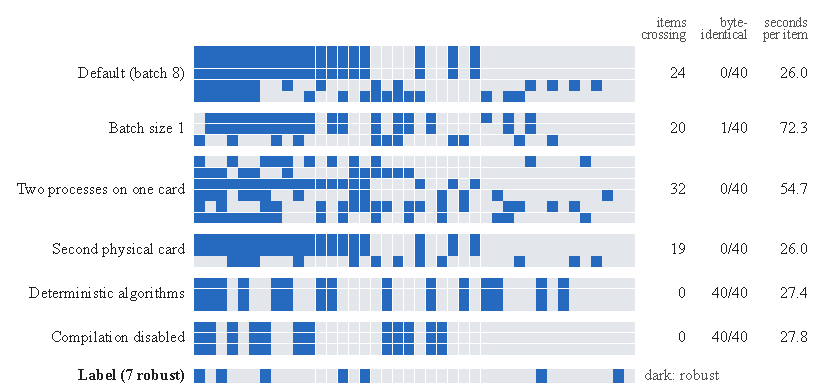
\includegraphics[width=\linewidth]{fig_rumore.pdf}
\caption{Predictions of the official pipeline for 40 preliminary public problems (columns) in 23 executions on DeepSeek (rows), by configuration; the last row is the label, dark cells are robust, and columns are sorted by how often they are predicted robust. At right: items whose prediction changes across the configuration's runs (more runs, more crossings), items whose generated text is byte-identical in all of them, and seconds per item.}
\label{fig:noise}
\end{figure}

\begin{table}[t]
\caption{Repeatability of the official pipeline on DeepSeek, 40 public problems, by configuration, in the order of Figure~\ref{fig:noise}. ``Crossings'': items whose prediction changes across the configuration's runs. ``Identical'': items whose generated text is byte-identical in all runs. Cost is runtime against the default configuration. Card 0 and card 1 are the two GPUs of the same machine. With two processes on one card, any five of its six runs give 29 to 31 crossings.}
\label{tab:reexec}
\centering
\small
\begin{tabular}{@{}lllllll@{}}
\toprule
\textbf{Configuration} & \textbf{Card} & \textbf{Runs} & \textbf{Crossings} & \textbf{Identical} & \textbf{Correct per run} & \textbf{Cost} \\
\midrule
Default (batch 8) & 0 & 5 & 24/40 & 0/40 & 24, 24, 24, 23, 24 & reference \\
Batch size 1 & 0 & 3 & 20/40 & 1/40 & 20, 21, 24 & +178\% \\
Two processes on one card & 0 & 6 & 32/40 & 0/40 & 24 to 28 & +110\% \\
Second physical card & 1 & 3 & 19/40 & 0/40 & 24, 24, 21 & +0\% \\
Deterministic algorithms & 0 & 3 & 0/40 & 40/40 & 24, 24, 24 & +5\% \\
Compilation disabled & 1 & 3 & 0/40 & 40/40 & 25, 25, 25 & +7\% \\
\bottomrule
\end{tabular}
\end{table}

\paragraph{Two candidate remedies.} Deterministic algorithms (PyTorch's, in warn-only mode, with deterministic cuDNN and a fixed cuBLAS workspace; Appendix~\ref{app:C}) and disabled compilation each made the generated text byte-identical in three sequential runs, at 5 to 7\% runtime cost. On card 0, the default configuration produced 24 crossings in five runs. Each remedy ran on one card where the default had produced crossings, each run in a new process, with no other process on that card. Three identical runs are weak evidence: the default configuration also gave three identical runs on card 0 before its fourth diverged, and five of its eight runs on the two cards shared one output. The two remedies produced different outputs, predicting 15 and 12 of the 40 problems robust, and because they ran on different cards we cannot tell whether the difference comes from the configuration or from the card. Neither gained more than one item (24 and 25 correct).

\paragraph{Distinct outputs.} The 23 executions fall into 14 distinct outputs, byte-identical within each. The same output appeared on both cards, and two runs launched in the same second on one card produced different outputs, so the output is not a property of the card alone; what selects it is not established. As only 7 of the 40 problems are robust and crossings largely cancel, accuracy moved much less than predictions: 21 to 24 correct in the default configuration on either card and 24 to 28 with two processes on one card, always below the 33 of the majority constant. An exploratory repetition of the official score extraction, whose third run ranks the 164 labeled problems at Spearman 0.24 against the first two, is in Appendix~\ref{app:C}.

\section{Regenerating the labels with our own protocol}\label{sec:labels}

\paragraph{Our labeling protocol.} We identified the organizers' perturbation families in the preliminary data (rephrase, rename, domain, distract, typos), regenerated them with gpt-oss-120b prompted with public examples, and gated each variant with gpt-oss-120b. An answer counts as correct when it matches gpt-oss-120b's answer on the original problem, because the preliminary data carry no answers; we did not check this key against the answers of the collections the problems come from. On the organizers' machine, with vLLM 0.28.0 [8] outside the official image, we labeled four models with two independent draws of variants (A and B, about 40 accepted variants per problem): 10 samples on the base problem and one per variant, at temperature 0.6, top-p 0.95 and at most 16,384 new tokens. Draw A's variants were also re-sampled with a new seed (A$'$). A label is robust when at least 6 of the 10 base samples are correct and every variant is answered correctly; unlike the earlier rule's conjunction, this requires the base problem to be solved.

A chain that reaches our cap is scored by the last boxed answer it contains, and counts as wrong without one; the organizers also count a response that reaches their limit without a parseable final answer as wrong [4]. Our protocol differs from the organizers' in perturbations, answer key, rule and sampling (one answer per variant, against 10 in the files behind most of their DeepSeek labels). Its decoding differs from the settings they publish, and its prompt may differ from the one behind their labels, which they have not stated.

\begin{table}[t]
\caption{Agreement of labels regenerated with our protocol: Cohen's kappa. The three columns for A and B treat variant chains that reached the 16,384-token cap in three ways: scored as in the protocol (by their last boxed answer, if any), dropped, or all counted as correct. The first of these columns and the A and A$'$ column give 95\% percentile bootstrap intervals over problems, and the script of Appendix~\ref{app:E} gives them for the other two. A problem has a label in a draw when it has at least one accepted variant (160 in A, 159 in B). Kappa between A and B uses the 159 problems labeled in both (150 for Qwen3.5-4B and 156 for DeepSeek when truncated chains are dropped), and between A and A$'$ 160. ``At cap'': percentage of variant chains that reached the cap in draws A and B. ``Robust'': percentage of problems labeled robust in draw A, as scored. The last column gives kappa of draw A with the organizers' preliminary DeepSeek labels: on the 138 published ones, and on the 160 that include 22 labels we derived (Section~\ref{sec:data}).}
\label{tab:label}
\centering
\small
\setlength{\tabcolsep}{3pt}
\begin{tabular}{@{}llllllll@{}}
\toprule
& & & \multicolumn{3}{l}{\textbf{A and B, truncated variant chains}} & & \\
\cmidrule(lr){4-6}
\textbf{Model} & \textbf{At cap} & \textbf{Robust} & \textbf{as scored} & \textbf{dropped} & \textbf{correct} & \textbf{A and A$'$} & \textbf{Organizers'} \\
\midrule
Skywork & 1.2, 1.5 & 74 & 0.44 [0.28, 0.59] & 0.39 & 0.39 & 0.79 [0.67, 0.89] & none \\
DeepSeek & 5.1, 6.1 & 39 & 0.41 [0.26, 0.55] & 0.35 & 0.36 & 0.46 [0.33, 0.59]$^{*}$ & 0.011; 0.025 \\
Olmo & 1.1, 0.9 & 68 & 0.38 [0.21, 0.54] & 0.39 & 0.39 & 0.65 [0.52, 0.78] & none \\
Qwen3.5-4B & 22.1, 29.2 & 9 & 0.18 [$-$0.06, 0.39] & 0.26 & 0.44 & not run & none \\
\bottomrule
\end{tabular}
\par\smallskip{\footnotesize $^{*}$On DeepSeek, A$'$ also received the answer-format line (end of this section), so this entry mixes seed and prompt.}
\end{table}

\paragraph{Results.} Under our protocol, two independent draws of variants give labels that agree at kappa 0.35 to 0.44 on Skywork, Olmo and DeepSeek, whether truncated variant chains are scored as in the protocol, dropped or all counted as correct (Table~\ref{tab:label}). On Qwen3.5-4B, 22 to 29\% of the variant chains reach the cap. Scoring these chains as in the protocol, dropping them or counting them all as correct gives agreement of 0.18, 0.26 and 0.44, and a robust share in draw A of 9\%, 83\% and 79\%. On Skywork, re-sampling the same variants with a new seed agrees far more than drawing new variants (0.79 against 0.44), so its label depends more on the variants than on the seed; on Olmo the gap is smaller (0.65 against 0.38), and on DeepSeek, where A$'$ also changed the prompt, it is 0.46 against 0.41.

Draw A's DeepSeek labels agree with the 138 labels the organizers published at kappa 0.011 [$-$0.13, 0.17], and with the 160 that include 22 of our derived labels at 0.025 [$-$0.12, 0.18]. Of the 36 problems with a published robust label, draw A calls 20 non-robust, and 4 of these change when truncated variants all count as correct. Of the 102 with a published non-robust label, draw A calls 44 robust. The reliability of the organizers' labels remains unmeasured. A retrospective calculation on the same saved answers with the main-phase threshold rule, applied as its pre-registration fixed it, with no filter on the base problem (Appendix~\ref{app:C}), gives test-retest point estimates between 0.34 and 0.56, below the pre-registered bar of 0.60, though three of the four intervals include it.

\paragraph{The prompt changes our labels.} In a first run with the bare problem text, later discarded, \mbox{Qwen3.5-4B} gave a final answer in the expected format in only 5 of its 1,640 base samples in draw A. With one instruction line requesting the format, 145 of 164 problems passed the base condition, against none. DeepSeek passed it on 147 of 164 with or without that line; its draws A and B ran without the line and A$'$ with it, and on the same variants its robust share moved from 39\% to 51\% of the 160 labeled problems, a change that mixes prompt and seed. Under our protocol, the label of Qwen3.5-4B therefore depends on the prompt. Whether this affects the organizers' labels is unknown: their baselines repository has a solve prompt that asks for an ANSWER line, but they have not said whether it was used for labeling (R3).

\section{The falsification campaign}\label{sec:campaign}

Table~\ref{tab:campaign} summarizes the campaign; Appendix~\ref{app:A} lists all 31 entries and explains three traps (rule T, the oracle H13, the duplicated pairs behind H2) and two pitfalls of the data. All entries use the preliminary data, except H16 to H18, which were scored on the 17 items of the warmup evaluation task.

\begin{table}[t]
\caption{The campaign in brief, in 19 of its 31 entries (Appendix~\ref{app:A} lists all). Ground truth is DeepSeek's and the preliminary pairs' unless stated; accuracy differences are in points against each pre-registration's baseline. H1, H7 and T count the 52 duplicated DeepSeek pairs twice; counted once, no verdict changes.}
\label{tab:campaign}
\centering
\small
\begin{tabular}{@{}L{5.5cm}L{1.9cm}L{5.6cm}@{}}
\toprule
\textbf{What we tested} & \textbf{Entries} & \textbf{Outcome} \\
\midrule
Text features; robustness as a property of the problem; labels, base accuracy and difficulty order across models & H1 to H5, H7 & rejected; H2 gained only when the duplicated pairs were counted twice \\
Official uncertainty features, logistic regression & H10 & 0.774 against a majority constant of 0.756, within the 0.692 $\pm$ 0.101 of the proposal [1] (method substituted) \\
Features cached for other models; per-target thresholds & H12, H13 & H12 rejected; the H13 ceiling withdrawn, $-$2.8 points when forced to rank \\
Our perturbation families, translation, self-consistency, the organizers' families regenerated (pilot), representation shift & H19, H22, H30 to H33 & rejected: kappa at most 0.02, AUROC at most 0.615 \\
Probes on DeepSeek's hidden states: ours and the organizers' published artifact & H36, H35 & survive their nulls; ours adds no detectable gain over length, and the artifact's score is probably in-sample \\
Trivial-robust rule, post hoc & T & a trap: +6.0 points on the preliminary pairs, +0.0 on \texttt{val-sample} \\
Identical bundles re-executed (warmup, 17 items) & H18 & noise confirmed: 11, 9, 11 and 11 correct \\
\bottomrule
\end{tabular}
\end{table}

\paragraph{Length and probes.} The character count of the problem alone orders the 164 DeepSeek labels at AUROC 0.704. Our logistic probe on DeepSeek's last-token hidden states, with layer and regularization chosen by inner cross-validation, reaches 0.710 out of fold with the original fold assignment. Over 20 other assignments, passed through the second-stage model below, it gives 0.57 to 0.76 (mean 0.69). Its scores correlate with length at Spearman +0.55, and residualized on log character count it gives 0.62. Its permutation null, rerun with 1{,}000 permutations of the whole nested procedure (the first version used 60, where 500 were pre-registered), gives $p = 0.002$. Restricted to the 138 published labels, these out-of-fold scores give 0.714 and length 0.733; retrained on those 138 alone with H36's procedure and seed, the probe gives 0.620. Combined with length in a second-stage model fitted on common outer folds, the probe changes AUROC over length alone by +0.005 on the 164 labels and by $-$0.010 on the 138 published ones (median bounds of the per-assignment 95\% intervals: $-$0.03 to 0.04, and $-$0.04 to 0.02): we detect no gain from adding the probe to length (Appendix~\ref{app:C}). This analysis replaces an earlier combination that leaked labels (Appendix~\ref{app:D}).

The organizers' published DeepSeek probe artifact orders the 164 DeepSeek labels at 0.739 with the aggregation we pre-registered and at 0.709 with its own, and at 0.62 and 0.57 residualized on log character count; its controls trained on shuffled labels give 0.68 at layer 31. The artifact does not record its training data; we infer that 137 of the 164 problems were among the public rows it was trained on, so these scores are probably largely in-sample. These length controls, which play the role of control tasks [7], were post hoc. Whether either probe reads anything beyond length that bears on robustness is not established. Apart from the three traps of Appendix~\ref{app:A}, no signal we scored by accuracy beats the majority constant by more than about one standard error on the preliminary labels, most of them DeepSeek's.

\section{Our entries}\label{sec:entries}

Our entry V8, pre-registered on 13 September, is the whole rule \texttt{return~[len(p)~>=~98 for~p~in~problems]}, with the threshold at the lower median of the 174 preliminary problems and the direction fixed on the preliminary pairs. On the original main-phase tasks it scored 11/21 and 10/19, like our entry v6 and the organizers' own entries. None of these beat the majority constant, which scores at least 11/21 and 10/19 on these tasks, and on so few items the ties do not show that length carries no signal (95\% Wilson intervals 0.32 to 0.72 and 0.32 to 0.73). On the 71 labeled rows of the official training set (revision of 17 September; 36 distinct problems), V8 differs from the all-robust constant on only 6 rows and is wrong on all 6 (46/71 against 52/71): too few to say what length is worth on official data. On the replacement tasks of 16 September, before and after the evaluation changed on 15 October [6], it predicted robust for every item (10/21 and 7/14), like an all-robust control. For the final test we nominated V8 (Codabench 1016713) and the constant (1016732), both on the Main track; our pre-registered predictions will be scored there (Appendix~\ref{app:B}).

\section{Recommendations}\label{sec:recs}

These rest mostly on DeepSeek and the preliminary data, and should be checked on the other models.
\begin{itemize}
\item \textbf{R1. Remove the variation between runs, and test the remedy:} on the same card with independent restarts, under load and across cards.
\item \textbf{R2. Repeat only where it decides something:} at the warmup's re-execution noise (a standard deviation of 1.0 item on 17, itself estimated from four runs), a one-item gap needs about eight runs per entry to reach two standard errors, so repeat only entries that run a model and sit near a prize boundary.
\item \textbf{R3. Say which prompt and decoding settings produced each released label file,} at least after the close.
\item \textbf{R4. Measure the label's reliability directly,} with two independent draws of variants labeled by the official process.
\item \textbf{R5. Show floors and noise on the leaderboard:} a row per constant predictor, the re-execution noise and binomial intervals.
\item \textbf{R6. Require a length control in white-box ablations.}
\item \textbf{R7. Remove the leaking field} \texttt{permutation\_type} from the aggregated datasets (Appendix~\ref{app:A}).
\end{itemize}

\paragraph{Code and data.} Our code, bundles, pre-registrations and outcome files are released at \href{https://github.com/Dan23RR/aimo-instrument}{\nolinkurl{github.com/Dan23RR/aimo-instrument}}. Its folder \texttt{reproduce/} recomputes the main tables from saved outputs and the six preliminary datasets, and the other numbers come from the dated records in \texttt{archive/} (Appendix~\ref{app:E}).

%%%%%% End of the main text: the six pages end here; the Limitations do not count %%%%%%
\label{fine-testo}

\section*{Limitations}

\begin{enumerate}[leftmargin=1.6em, itemsep=2pt, topsep=4pt, parsep=0pt]
\item \textbf{Preliminary data, not official data.} We did not repeat our label and probe analyses on the official training set, beyond the evaluation of V8 and a five-row check of our labels (Appendix~\ref{app:C}). Findings on label reliability and predictability may not generalize to the official evaluation setting.
\item \textbf{Our protocol, not the official one.} We did not regenerate labels with the organizers' published settings (100,000 tokens, temperature 1.0), with 10 answers per variant as in the files behind most DeepSeek labels, or on \texttt{train-main-v2}. The three treatments of truncated variant chains show how much our cap moves agreement between our draws; all three score base samples that reach the cap as the protocol does, and none of them reproduces longer decoding or a different temperature. Our low agreement with the organizers' labels is a fact about our process.
\item \textbf{One model.} We ran the probes, the re-execution study of Section~\ref{sec:reexec} and the comparisons of our regenerated labels with the organizers' preliminary labels only on DeepSeek.
\item \textbf{Re-execution.} We did not run the two candidate remedies on the same card, so card and configuration are confounded; we did not test either remedy under contention or on both cards, and we used 40 problems and one image.
\item \textbf{Records.} Some analyses rest on re-created scripts or dated records (Appendix~\ref{app:D}). Nothing here estimates performance on the final held-out problems.
\end{enumerate}

\section*{AI usage statement}

In this work, we used one generative AI tool, Claude (Anthropic), through Claude Code, for ideation, coding, analysis and writing. Ideation: it drafted the pre-registrations, including hypotheses, predictions and kill criteria, and searched and summarized the literature and the public records, including the organizers' Discord channels and the author's correspondence with them. Coding: it wrote the solution code of our bundles and the analysis and extraction scripts, ran them, and operated the organizers' virtual machine over SSH. Analysis: it computed and interpreted the results and ran automated adversarial reviews of hypotheses, drafts and code. Writing: it drafted the correspondence, this report and its revision after review.

It also made most of our Codabench uploads through the author's browser at the author's instruction. There were two exceptions: one resubmission (925822, 14 September), made without a specific instruction, and one submission that the author had not approved, sent in error and rejected before import (1016734, 28 October).

Language models were also components of our method: gpt-oss-120b generated and gated the perturbation variants and supplied the reference answers of Section~\ref{sec:labels}, and phi-4 translated problems for H22. The final decisions on the direction of the work, on the submissions (with the two exceptions above), on the nominations for the final test and on the claims of this report were the author's, and the author sent all correspondence personally. The author has reviewed all AI-assisted work and takes full responsibility for the final content of this report.

\begin{ack}
We thank Michal Štefánik, Róbert Belanec and the AIMO Interpretability team for the compute grant, a virtual machine with two GPUs, and for answering our questions; on 2 November they confirmed that the measurements taken on their machine may appear in this report. We also thank the three reviewers and the program chairs: two reviewers checked our analyses against the released code and data, and their checks corrected several of our claims. Other GPU time was rented on Modal and paid by the author or covered by Modal's platform credit. This work received no other funding, and the author has no competing interests.
\end{ack}

\section*{References}
{\small
[1] M. Štefánik, P. Mondorf, A. Waldis, Q. Liu, C. Yang, M. Spiegel, J. Kuchař, M. Kadlčík, A. Vawda-Oomerjee, C. Liu, S. Frieder, B. Plank, F. Barez and P. Stenetorp. AIMO Interpretability Challenge. CoRR, abs/2607.13899, 2026. doi:10.48550/arXiv.2607.13899.

[2] H. He and Thinking Machines Lab. Defeating Nondeterminism in LLM Inference. Thinking Machines Lab: Connectionism, 2025.

[3] J. Yuan, H. Li, X. Ding, W. Xie, Y.-J. Li, W. Zhao, K. Wan, J. Shi, X. Hu and Z. Liu. Understanding and Mitigating Numerical Sources of Nondeterminism in LLM Inference. NeurIPS 2025. arXiv:2506.09501.

[4] AIMO Interpretability Challenge website and FAQ. \url{https://aimo-interp.github.io} (accessed 28 October 2026), and its source repository aimo-interp/aimo-interp.github.io on GitHub.

[5] aimo-interp/getting-started and aimo-interp/baselines, GitHub repositories: README and issues \#6 and \#10 of getting-started; aimo-interp datasets on Hugging Face, including \texttt{train-main-v2} and \texttt{val-sample}.

[6] AIMO Interpretability Challenge Discord, \#announcements and \#qa: 5, 15 and 22 September, 9, 15, 16 and 20 October 2026.

[7] J. Hewitt and P. Liang. Designing and Interpreting Probes with Control Tasks. EMNLP-IJCNLP 2019.

[8] W. Kwon et al. Efficient Memory Management for Large Language Model Serving with PagedAttention. SOSP 2023.

[9] D. Hendrycks et al. Measuring Mathematical Problem Solving With the MATH Dataset. NeurIPS 2021 Datasets and Benchmarks Track. arXiv:2103.03874.
}

%%%%%% End of the references %%%%%%
\clearpage
\appendix
\raggedright

\input{app_A}
\input{app_B}
\input{app_C}
\input{app_D}
\input{app_E}

\newpage
\input{checklist_compilata.tex}

\end{document}
".
%% Every line numbered (same numbering, used to find the lines cited in the note): "\def\everyline{}\documentclass{article}

%% Conditional revision of November 2026: six pages of main text, from the title to the end of Section 7 (label
%% fine-testo); the Limitations, the AI usage statement, the references and the appendices do not count.
%% Final mode with the workshop name. Line numbers on every fifth line, small and grey, for the note to the
%% program chairs, who asked for section and line numbers. Copy without them: pdflatex "\def\cleancopy{}\input{main}".
%% Every line numbered (same numbering, used to find the lines cited in the note): "\def\everyline{}\input{main}".
\usepackage[final,sglblindworkshop]{neurips_2026}
\workshoptitle{AIMO Interpretability Challenge}
\ifdefined\cleancopy\else
  \usepackage{lineno}
  \linenumbers
  \ifdefined\everyline\else\modulolinenumbers[5]\fi
  \renewcommand\linenumberfont{\normalfont\tiny\sffamily\color{black!45}}
\fi

\usepackage[utf8]{inputenc}
\usepackage[T1]{fontenc}
%% Typewriter text in Latin Modern, the Type 1 version of the default Computer Modern typewriter, with the same
%% widths: without it, \texttt in T1 encoding becomes bitmap (Type 3) fonts, and the template asks for Type 1 fonts.
\renewcommand{\ttdefault}{lmtt}
\usepackage{hyperref}
\hypersetup{pdftitle={The Instrument Behind the Leaderboard: Re-Execution Noise and Label Regeneration in the AIMO Interpretability Challenge}, pdfauthor={Daniel Culotta}}
\usepackage{url}
\def\UrlBreaks{\do\/\do\.\do\_\do\-\do\:}
\usepackage{booktabs}
\usepackage{array}
\usepackage{longtable}
\newcolumntype{L}[1]{>{\raggedright\arraybackslash}p{#1}}
\usepackage{amsfonts}
\usepackage{microtype}
\usepackage{xcolor}
\usepackage{graphicx}
\usepackage{enumitem}
\usepackage{needspace}
\setlist[itemize]{leftmargin=1.4em, itemsep=2pt, topsep=4pt, parsep=0pt}
\setlist[itemize,2]{label=$\circ$}
\renewcommand{\arraystretch}{1.15}
\raggedbottom

\title{The Instrument Behind the Leaderboard: Re-Execution Noise and Label Regeneration in the AIMO Interpretability Challenge}

\author{%
  Daniel Culotta \\
  Independent researcher
}

\begin{document}

\maketitle

\begin{abstract}
We treat the AIMO Interpretability benchmark, which asks whether a model's answer to a math problem survives perturbations, as a measurement instrument. Almost all our label and probe analyses use the preliminary datasets. As the program chairs note, these differ from the official training and validation data in sampling, perturbations and eligibility, so findings on label reliability and predictability may not hold in the official evaluation. First, on DeepSeek-R1-0528-Qwen3-8B in the official pipeline, 24 of 40 items changed prediction across five default runs. Turning compilation off, or deterministic algorithms on, gave three byte-identical runs, each on one card. Second, we regenerated labels with our own protocol, not the official one: our perturbations and answer key, one answer per variant, a 16,384-token cap and temperature 0.6, where the organizers publish 100,000 tokens and 1.0. Two independent draws agree at kappa 0.35 to 0.44 on three of four models however truncated chains are treated, and 0.18 to 0.44 on Qwen3.5-4B, whose chains often reach the cap. Draw A agrees with the 138 published DeepSeek labels at kappa 0.01. This describes our protocol and does not measure the reliability of the organizers' labels. Third, of the 27 dated hypotheses with a kill criterion, 21 failed it. Our probe on DeepSeek's hidden states does no better than problem length (AUROC 0.710 against 0.704; below length on the published labels) and adds nothing detectable to it.
\end{abstract}

\section{Introduction}\label{sec:1}

A leaderboard is a measurement. Its score is read off an instrument made of a label, an evaluation set, an inference pipeline and the hardware it runs on. When the label is itself produced by a stochastic process, the instrument has noise of its own, which a single submission cannot see. We measure the re-execution noise of the official extraction and regressor, and the repeatability of labels regenerated with our own protocol, not the noise of the organizers' labels.

We study the instrument of the AIMO Interpretability Challenge, in which a submission predicts, for a given model and math problem, whether the model's answer is robust to perturbations of the problem [1]. We ran our work as a falsification campaign: every hypothesis was recorded in a dated file, 26 of the 31 before their data were seen, and every tested hypothesis is reported. Of the 31 entries, 27 carried a kill criterion written before their test ran (for 3 of them in a written plan rather than a frozen pre-registration, and for H2 after its concordance had been seen). By that criterion 21 were rejected, 5 survived and 1 is not established (Appendix~\ref{app:A}).

\paragraph{Scope.} Three limits apply.
\begin{itemize}
\item \textbf{Preliminary and official data.} Almost all of our label and probe analyses use the six preliminary public datasets released before the main phase. Their labels follow an earlier rule than those of the official training set (\texttt{train-main-v2}) and of the validation and test tasks [5]; as the program chairs noted in their meta-review, their sampling procedures, perturbations and eligibility criteria also differ. Beyond the label rule, we did not compare the two. Unless we say otherwise, a result on labels or on their predictability holds for the preliminary data and may not hold in the official evaluation setting.
\item \textbf{Our labeling protocol is not the official one.} When we regenerate labels (Section~\ref{sec:labels}), we use our own perturbations, prompts, sampling, decoding, answer key and labeling rule. Disagreement with the organizers' preliminary labels therefore shows that the two processes give different labels; it does not establish that their labels are unreliable or irreproducible.
\item \textbf{Mostly one model.} The re-execution study of Section~\ref{sec:reexec}, the probe analyses and every comparison of our regenerated labels with the organizers' preliminary labels are on DeepSeek-R1-0528-Qwen3-8B. Regenerated labels cover four models, but no conclusion about the official benchmark is established across models.
\end{itemize}

Within these limits, Sections~\ref{sec:reexec} to~\ref{sec:campaign} report re-execution noise and two candidate remedies, our regenerated labels, and signals that do no better than problem length or come from an artifact of the data. Nondeterminism of LLM inference is documented in general [2, 3]; we add its size for one model, one submission and 40 problems on this benchmark's hardware and pipeline. We make no claim about any participant's method.

\section{The task, the labels and the data}\label{sec:data}

\paragraph{Task.} A submission receives a model identifier, a reasoning effort and a list of problems, and returns one robustness verdict per problem, offline on one GPU within one hour [4, 5], or 70 minutes since 15 October [6]. The models are Qwen3.5-4B, Skywork-OR1-Math-7B, Olmo-3-7B-Think and \mbox{DeepSeek-R1-0528-Qwen3-8B} in both tracks, and gpt-oss-120b in the Main track only.

\paragraph{Official data.} The main-phase training set \texttt{train-main-v2} labels all five models with a threshold on the largest accuracy drop across perturbation families: robust at most 0.10, non-robust at least 0.25, no label in between [5]. The organizers' published decoding settings are up to 100,000 tokens at temperature 1.0, top-k 40 and top-p 0.95, and a response that reaches the limit without a final answer counts as wrong [4]. Since 16 September the private validation tasks have 21 items (Main) and 14 (Small), on which the binomial standard error of an accuracy near one half is 10.9 and 13.4 points; the final test uses 30 to 50 new problems [5, 6].

\paragraph{Preliminary data.} Six datasets released before the main phase aggregate to 335 (model, problem) pairs over 174 distinct problems, up to eight per problem; 52 pairs repeat the DeepSeek measurements under a second model name. Their labels follow an earlier rule: on all 379 labeled rows (a pair can have several), the label equals the conjunction ``no perturbation lowered accuracy''. A per-family majority rule (``more than half of the answers are correct in every perturbation family'') reproduces the same 379 labels, so these rows cannot tell the two rules apart. Whether they used the decoding settings above is not documented; in the files behind most DeepSeek labels, most variants listed as lowering accuracy were answered 10 times. We call their labels the organizers' preliminary labels, and keep ``official'' for \texttt{train-main-v2} and the validation and test tasks.

\paragraph{DeepSeek labels.} DeepSeek is the only evaluated model with many preliminary labels: 164 distinct problems (the 52 duplicated pairs count once). For 138 of them the data publish a label. For the other 26 we derived one with the conjunction, which makes 4 of them robust; the majority rule would make 21 robust, so these 26 labels depend on the choice of rule. We therefore report results on the 138 published labels separately.

\section{Re-execution noise on the evaluation workers' type of GPU}\label{sec:reexec}

On a virtual machine lent by the organizers, with two NVIDIA RTX PRO 6000 Blackwell Server Edition GPUs (the type the evaluation workers use), we ran 40 preliminary public problems through the official runtime image, extraction and regressor, unmodified, on DeepSeek. Decoding was greedy, with at most 4,096 new tokens in batches of 8. The 40 labels are DeepSeek's of Section~\ref{sec:data}: 28 published and 12 that we derived with the conjunction, which include 3 of the 7 robust ones. Figure~\ref{fig:noise} shows the 23 executions; Table~\ref{tab:reexec} gives the repeatability of each configuration.

\begin{figure}[t]
\centering
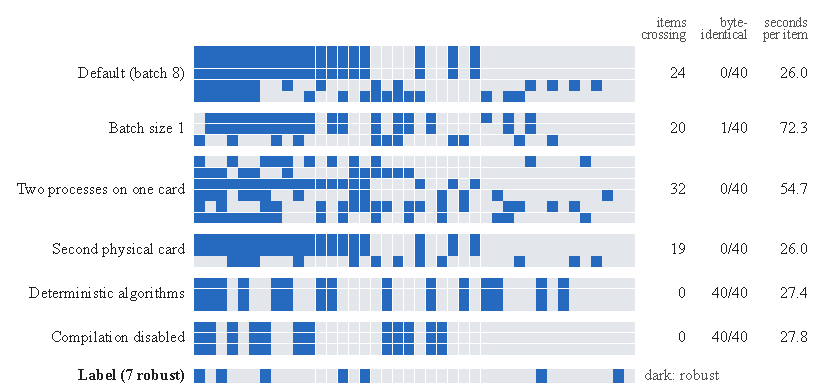
\includegraphics[width=\linewidth]{fig_rumore.pdf}
\caption{Predictions of the official pipeline for 40 preliminary public problems (columns) in 23 executions on DeepSeek (rows), by configuration; the last row is the label, dark cells are robust, and columns are sorted by how often they are predicted robust. At right: items whose prediction changes across the configuration's runs (more runs, more crossings), items whose generated text is byte-identical in all of them, and seconds per item.}
\label{fig:noise}
\end{figure}

\begin{table}[t]
\caption{Repeatability of the official pipeline on DeepSeek, 40 public problems, by configuration, in the order of Figure~\ref{fig:noise}. ``Crossings'': items whose prediction changes across the configuration's runs. ``Identical'': items whose generated text is byte-identical in all runs. Cost is runtime against the default configuration. Card 0 and card 1 are the two GPUs of the same machine. With two processes on one card, any five of its six runs give 29 to 31 crossings.}
\label{tab:reexec}
\centering
\small
\begin{tabular}{@{}lllllll@{}}
\toprule
\textbf{Configuration} & \textbf{Card} & \textbf{Runs} & \textbf{Crossings} & \textbf{Identical} & \textbf{Correct per run} & \textbf{Cost} \\
\midrule
Default (batch 8) & 0 & 5 & 24/40 & 0/40 & 24, 24, 24, 23, 24 & reference \\
Batch size 1 & 0 & 3 & 20/40 & 1/40 & 20, 21, 24 & +178\% \\
Two processes on one card & 0 & 6 & 32/40 & 0/40 & 24 to 28 & +110\% \\
Second physical card & 1 & 3 & 19/40 & 0/40 & 24, 24, 21 & +0\% \\
Deterministic algorithms & 0 & 3 & 0/40 & 40/40 & 24, 24, 24 & +5\% \\
Compilation disabled & 1 & 3 & 0/40 & 40/40 & 25, 25, 25 & +7\% \\
\bottomrule
\end{tabular}
\end{table}

\paragraph{Two candidate remedies.} Deterministic algorithms (PyTorch's, in warn-only mode, with deterministic cuDNN and a fixed cuBLAS workspace; Appendix~\ref{app:C}) and disabled compilation each made the generated text byte-identical in three sequential runs, at 5 to 7\% runtime cost. On card 0, the default configuration produced 24 crossings in five runs. Each remedy ran on one card where the default had produced crossings, each run in a new process, with no other process on that card. Three identical runs are weak evidence: the default configuration also gave three identical runs on card 0 before its fourth diverged, and five of its eight runs on the two cards shared one output. The two remedies produced different outputs, predicting 15 and 12 of the 40 problems robust, and because they ran on different cards we cannot tell whether the difference comes from the configuration or from the card. Neither gained more than one item (24 and 25 correct).

\paragraph{Distinct outputs.} The 23 executions fall into 14 distinct outputs, byte-identical within each. The same output appeared on both cards, and two runs launched in the same second on one card produced different outputs, so the output is not a property of the card alone; what selects it is not established. As only 7 of the 40 problems are robust and crossings largely cancel, accuracy moved much less than predictions: 21 to 24 correct in the default configuration on either card and 24 to 28 with two processes on one card, always below the 33 of the majority constant. An exploratory repetition of the official score extraction, whose third run ranks the 164 labeled problems at Spearman 0.24 against the first two, is in Appendix~\ref{app:C}.

\section{Regenerating the labels with our own protocol}\label{sec:labels}

\paragraph{Our labeling protocol.} We identified the organizers' perturbation families in the preliminary data (rephrase, rename, domain, distract, typos), regenerated them with gpt-oss-120b prompted with public examples, and gated each variant with gpt-oss-120b. An answer counts as correct when it matches gpt-oss-120b's answer on the original problem, because the preliminary data carry no answers; we did not check this key against the answers of the collections the problems come from. On the organizers' machine, with vLLM 0.28.0 [8] outside the official image, we labeled four models with two independent draws of variants (A and B, about 40 accepted variants per problem): 10 samples on the base problem and one per variant, at temperature 0.6, top-p 0.95 and at most 16,384 new tokens. Draw A's variants were also re-sampled with a new seed (A$'$). A label is robust when at least 6 of the 10 base samples are correct and every variant is answered correctly; unlike the earlier rule's conjunction, this requires the base problem to be solved.

A chain that reaches our cap is scored by the last boxed answer it contains, and counts as wrong without one; the organizers also count a response that reaches their limit without a parseable final answer as wrong [4]. Our protocol differs from the organizers' in perturbations, answer key, rule and sampling (one answer per variant, against 10 in the files behind most of their DeepSeek labels). Its decoding differs from the settings they publish, and its prompt may differ from the one behind their labels, which they have not stated.

\begin{table}[t]
\caption{Agreement of labels regenerated with our protocol: Cohen's kappa. The three columns for A and B treat variant chains that reached the 16,384-token cap in three ways: scored as in the protocol (by their last boxed answer, if any), dropped, or all counted as correct. The first of these columns and the A and A$'$ column give 95\% percentile bootstrap intervals over problems, and the script of Appendix~\ref{app:E} gives them for the other two. A problem has a label in a draw when it has at least one accepted variant (160 in A, 159 in B). Kappa between A and B uses the 159 problems labeled in both (150 for Qwen3.5-4B and 156 for DeepSeek when truncated chains are dropped), and between A and A$'$ 160. ``At cap'': percentage of variant chains that reached the cap in draws A and B. ``Robust'': percentage of problems labeled robust in draw A, as scored. The last column gives kappa of draw A with the organizers' preliminary DeepSeek labels: on the 138 published ones, and on the 160 that include 22 labels we derived (Section~\ref{sec:data}).}
\label{tab:label}
\centering
\small
\setlength{\tabcolsep}{3pt}
\begin{tabular}{@{}llllllll@{}}
\toprule
& & & \multicolumn{3}{l}{\textbf{A and B, truncated variant chains}} & & \\
\cmidrule(lr){4-6}
\textbf{Model} & \textbf{At cap} & \textbf{Robust} & \textbf{as scored} & \textbf{dropped} & \textbf{correct} & \textbf{A and A$'$} & \textbf{Organizers'} \\
\midrule
Skywork & 1.2, 1.5 & 74 & 0.44 [0.28, 0.59] & 0.39 & 0.39 & 0.79 [0.67, 0.89] & none \\
DeepSeek & 5.1, 6.1 & 39 & 0.41 [0.26, 0.55] & 0.35 & 0.36 & 0.46 [0.33, 0.59]$^{*}$ & 0.011; 0.025 \\
Olmo & 1.1, 0.9 & 68 & 0.38 [0.21, 0.54] & 0.39 & 0.39 & 0.65 [0.52, 0.78] & none \\
Qwen3.5-4B & 22.1, 29.2 & 9 & 0.18 [$-$0.06, 0.39] & 0.26 & 0.44 & not run & none \\
\bottomrule
\end{tabular}
\par\smallskip{\footnotesize $^{*}$On DeepSeek, A$'$ also received the answer-format line (end of this section), so this entry mixes seed and prompt.}
\end{table}

\paragraph{Results.} Under our protocol, two independent draws of variants give labels that agree at kappa 0.35 to 0.44 on Skywork, Olmo and DeepSeek, whether truncated variant chains are scored as in the protocol, dropped or all counted as correct (Table~\ref{tab:label}). On Qwen3.5-4B, 22 to 29\% of the variant chains reach the cap. Scoring these chains as in the protocol, dropping them or counting them all as correct gives agreement of 0.18, 0.26 and 0.44, and a robust share in draw A of 9\%, 83\% and 79\%. On Skywork, re-sampling the same variants with a new seed agrees far more than drawing new variants (0.79 against 0.44), so its label depends more on the variants than on the seed; on Olmo the gap is smaller (0.65 against 0.38), and on DeepSeek, where A$'$ also changed the prompt, it is 0.46 against 0.41.

Draw A's DeepSeek labels agree with the 138 labels the organizers published at kappa 0.011 [$-$0.13, 0.17], and with the 160 that include 22 of our derived labels at 0.025 [$-$0.12, 0.18]. Of the 36 problems with a published robust label, draw A calls 20 non-robust, and 4 of these change when truncated variants all count as correct. Of the 102 with a published non-robust label, draw A calls 44 robust. The reliability of the organizers' labels remains unmeasured. A retrospective calculation on the same saved answers with the main-phase threshold rule, applied as its pre-registration fixed it, with no filter on the base problem (Appendix~\ref{app:C}), gives test-retest point estimates between 0.34 and 0.56, below the pre-registered bar of 0.60, though three of the four intervals include it.

\paragraph{The prompt changes our labels.} In a first run with the bare problem text, later discarded, \mbox{Qwen3.5-4B} gave a final answer in the expected format in only 5 of its 1,640 base samples in draw A. With one instruction line requesting the format, 145 of 164 problems passed the base condition, against none. DeepSeek passed it on 147 of 164 with or without that line; its draws A and B ran without the line and A$'$ with it, and on the same variants its robust share moved from 39\% to 51\% of the 160 labeled problems, a change that mixes prompt and seed. Under our protocol, the label of Qwen3.5-4B therefore depends on the prompt. Whether this affects the organizers' labels is unknown: their baselines repository has a solve prompt that asks for an ANSWER line, but they have not said whether it was used for labeling (R3).

\section{The falsification campaign}\label{sec:campaign}

Table~\ref{tab:campaign} summarizes the campaign; Appendix~\ref{app:A} lists all 31 entries and explains three traps (rule T, the oracle H13, the duplicated pairs behind H2) and two pitfalls of the data. All entries use the preliminary data, except H16 to H18, which were scored on the 17 items of the warmup evaluation task.

\begin{table}[t]
\caption{The campaign in brief, in 19 of its 31 entries (Appendix~\ref{app:A} lists all). Ground truth is DeepSeek's and the preliminary pairs' unless stated; accuracy differences are in points against each pre-registration's baseline. H1, H7 and T count the 52 duplicated DeepSeek pairs twice; counted once, no verdict changes.}
\label{tab:campaign}
\centering
\small
\begin{tabular}{@{}L{5.5cm}L{1.9cm}L{5.6cm}@{}}
\toprule
\textbf{What we tested} & \textbf{Entries} & \textbf{Outcome} \\
\midrule
Text features; robustness as a property of the problem; labels, base accuracy and difficulty order across models & H1 to H5, H7 & rejected; H2 gained only when the duplicated pairs were counted twice \\
Official uncertainty features, logistic regression & H10 & 0.774 against a majority constant of 0.756, within the 0.692 $\pm$ 0.101 of the proposal [1] (method substituted) \\
Features cached for other models; per-target thresholds & H12, H13 & H12 rejected; the H13 ceiling withdrawn, $-$2.8 points when forced to rank \\
Our perturbation families, translation, self-consistency, the organizers' families regenerated (pilot), representation shift & H19, H22, H30 to H33 & rejected: kappa at most 0.02, AUROC at most 0.615 \\
Probes on DeepSeek's hidden states: ours and the organizers' published artifact & H36, H35 & survive their nulls; ours adds no detectable gain over length, and the artifact's score is probably in-sample \\
Trivial-robust rule, post hoc & T & a trap: +6.0 points on the preliminary pairs, +0.0 on \texttt{val-sample} \\
Identical bundles re-executed (warmup, 17 items) & H18 & noise confirmed: 11, 9, 11 and 11 correct \\
\bottomrule
\end{tabular}
\end{table}

\paragraph{Length and probes.} The character count of the problem alone orders the 164 DeepSeek labels at AUROC 0.704. Our logistic probe on DeepSeek's last-token hidden states, with layer and regularization chosen by inner cross-validation, reaches 0.710 out of fold with the original fold assignment. Over 20 other assignments, passed through the second-stage model below, it gives 0.57 to 0.76 (mean 0.69). Its scores correlate with length at Spearman +0.55, and residualized on log character count it gives 0.62. Its permutation null, rerun with 1{,}000 permutations of the whole nested procedure (the first version used 60, where 500 were pre-registered), gives $p = 0.002$. Restricted to the 138 published labels, these out-of-fold scores give 0.714 and length 0.733; retrained on those 138 alone with H36's procedure and seed, the probe gives 0.620. Combined with length in a second-stage model fitted on common outer folds, the probe changes AUROC over length alone by +0.005 on the 164 labels and by $-$0.010 on the 138 published ones (median bounds of the per-assignment 95\% intervals: $-$0.03 to 0.04, and $-$0.04 to 0.02): we detect no gain from adding the probe to length (Appendix~\ref{app:C}). This analysis replaces an earlier combination that leaked labels (Appendix~\ref{app:D}).

The organizers' published DeepSeek probe artifact orders the 164 DeepSeek labels at 0.739 with the aggregation we pre-registered and at 0.709 with its own, and at 0.62 and 0.57 residualized on log character count; its controls trained on shuffled labels give 0.68 at layer 31. The artifact does not record its training data; we infer that 137 of the 164 problems were among the public rows it was trained on, so these scores are probably largely in-sample. These length controls, which play the role of control tasks [7], were post hoc. Whether either probe reads anything beyond length that bears on robustness is not established. Apart from the three traps of Appendix~\ref{app:A}, no signal we scored by accuracy beats the majority constant by more than about one standard error on the preliminary labels, most of them DeepSeek's.

\section{Our entries}\label{sec:entries}

Our entry V8, pre-registered on 13 September, is the whole rule \texttt{return~[len(p)~>=~98 for~p~in~problems]}, with the threshold at the lower median of the 174 preliminary problems and the direction fixed on the preliminary pairs. On the original main-phase tasks it scored 11/21 and 10/19, like our entry v6 and the organizers' own entries. None of these beat the majority constant, which scores at least 11/21 and 10/19 on these tasks, and on so few items the ties do not show that length carries no signal (95\% Wilson intervals 0.32 to 0.72 and 0.32 to 0.73). On the 71 labeled rows of the official training set (revision of 17 September; 36 distinct problems), V8 differs from the all-robust constant on only 6 rows and is wrong on all 6 (46/71 against 52/71): too few to say what length is worth on official data. On the replacement tasks of 16 September, before and after the evaluation changed on 15 October [6], it predicted robust for every item (10/21 and 7/14), like an all-robust control. For the final test we nominated V8 (Codabench 1016713) and the constant (1016732), both on the Main track; our pre-registered predictions will be scored there (Appendix~\ref{app:B}).

\section{Recommendations}\label{sec:recs}

These rest mostly on DeepSeek and the preliminary data, and should be checked on the other models.
\begin{itemize}
\item \textbf{R1. Remove the variation between runs, and test the remedy:} on the same card with independent restarts, under load and across cards.
\item \textbf{R2. Repeat only where it decides something:} at the warmup's re-execution noise (a standard deviation of 1.0 item on 17, itself estimated from four runs), a one-item gap needs about eight runs per entry to reach two standard errors, so repeat only entries that run a model and sit near a prize boundary.
\item \textbf{R3. Say which prompt and decoding settings produced each released label file,} at least after the close.
\item \textbf{R4. Measure the label's reliability directly,} with two independent draws of variants labeled by the official process.
\item \textbf{R5. Show floors and noise on the leaderboard:} a row per constant predictor, the re-execution noise and binomial intervals.
\item \textbf{R6. Require a length control in white-box ablations.}
\item \textbf{R7. Remove the leaking field} \texttt{permutation\_type} from the aggregated datasets (Appendix~\ref{app:A}).
\end{itemize}

\paragraph{Code and data.} Our code, bundles, pre-registrations and outcome files are released at \href{https://github.com/Dan23RR/aimo-instrument}{\nolinkurl{github.com/Dan23RR/aimo-instrument}}. Its folder \texttt{reproduce/} recomputes the main tables from saved outputs and the six preliminary datasets, and the other numbers come from the dated records in \texttt{archive/} (Appendix~\ref{app:E}).

%%%%%% End of the main text: the six pages end here; the Limitations do not count %%%%%%
\label{fine-testo}

\section*{Limitations}

\begin{enumerate}[leftmargin=1.6em, itemsep=2pt, topsep=4pt, parsep=0pt]
\item \textbf{Preliminary data, not official data.} We did not repeat our label and probe analyses on the official training set, beyond the evaluation of V8 and a five-row check of our labels (Appendix~\ref{app:C}). Findings on label reliability and predictability may not generalize to the official evaluation setting.
\item \textbf{Our protocol, not the official one.} We did not regenerate labels with the organizers' published settings (100,000 tokens, temperature 1.0), with 10 answers per variant as in the files behind most DeepSeek labels, or on \texttt{train-main-v2}. The three treatments of truncated variant chains show how much our cap moves agreement between our draws; all three score base samples that reach the cap as the protocol does, and none of them reproduces longer decoding or a different temperature. Our low agreement with the organizers' labels is a fact about our process.
\item \textbf{One model.} We ran the probes, the re-execution study of Section~\ref{sec:reexec} and the comparisons of our regenerated labels with the organizers' preliminary labels only on DeepSeek.
\item \textbf{Re-execution.} We did not run the two candidate remedies on the same card, so card and configuration are confounded; we did not test either remedy under contention or on both cards, and we used 40 problems and one image.
\item \textbf{Records.} Some analyses rest on re-created scripts or dated records (Appendix~\ref{app:D}). Nothing here estimates performance on the final held-out problems.
\end{enumerate}

\section*{AI usage statement}

In this work, we used one generative AI tool, Claude (Anthropic), through Claude Code, for ideation, coding, analysis and writing. Ideation: it drafted the pre-registrations, including hypotheses, predictions and kill criteria, and searched and summarized the literature and the public records, including the organizers' Discord channels and the author's correspondence with them. Coding: it wrote the solution code of our bundles and the analysis and extraction scripts, ran them, and operated the organizers' virtual machine over SSH. Analysis: it computed and interpreted the results and ran automated adversarial reviews of hypotheses, drafts and code. Writing: it drafted the correspondence, this report and its revision after review.

It also made most of our Codabench uploads through the author's browser at the author's instruction. There were two exceptions: one resubmission (925822, 14 September), made without a specific instruction, and one submission that the author had not approved, sent in error and rejected before import (1016734, 28 October).

Language models were also components of our method: gpt-oss-120b generated and gated the perturbation variants and supplied the reference answers of Section~\ref{sec:labels}, and phi-4 translated problems for H22. The final decisions on the direction of the work, on the submissions (with the two exceptions above), on the nominations for the final test and on the claims of this report were the author's, and the author sent all correspondence personally. The author has reviewed all AI-assisted work and takes full responsibility for the final content of this report.

\begin{ack}
We thank Michal Štefánik, Róbert Belanec and the AIMO Interpretability team for the compute grant, a virtual machine with two GPUs, and for answering our questions; on 2 November they confirmed that the measurements taken on their machine may appear in this report. We also thank the three reviewers and the program chairs: two reviewers checked our analyses against the released code and data, and their checks corrected several of our claims. Other GPU time was rented on Modal and paid by the author or covered by Modal's platform credit. This work received no other funding, and the author has no competing interests.
\end{ack}

\section*{References}
{\small
[1] M. Štefánik, P. Mondorf, A. Waldis, Q. Liu, C. Yang, M. Spiegel, J. Kuchař, M. Kadlčík, A. Vawda-Oomerjee, C. Liu, S. Frieder, B. Plank, F. Barez and P. Stenetorp. AIMO Interpretability Challenge. CoRR, abs/2607.13899, 2026. doi:10.48550/arXiv.2607.13899.

[2] H. He and Thinking Machines Lab. Defeating Nondeterminism in LLM Inference. Thinking Machines Lab: Connectionism, 2025.

[3] J. Yuan, H. Li, X. Ding, W. Xie, Y.-J. Li, W. Zhao, K. Wan, J. Shi, X. Hu and Z. Liu. Understanding and Mitigating Numerical Sources of Nondeterminism in LLM Inference. NeurIPS 2025. arXiv:2506.09501.

[4] AIMO Interpretability Challenge website and FAQ. \url{https://aimo-interp.github.io} (accessed 28 October 2026), and its source repository aimo-interp/aimo-interp.github.io on GitHub.

[5] aimo-interp/getting-started and aimo-interp/baselines, GitHub repositories: README and issues \#6 and \#10 of getting-started; aimo-interp datasets on Hugging Face, including \texttt{train-main-v2} and \texttt{val-sample}.

[6] AIMO Interpretability Challenge Discord, \#announcements and \#qa: 5, 15 and 22 September, 9, 15, 16 and 20 October 2026.

[7] J. Hewitt and P. Liang. Designing and Interpreting Probes with Control Tasks. EMNLP-IJCNLP 2019.

[8] W. Kwon et al. Efficient Memory Management for Large Language Model Serving with PagedAttention. SOSP 2023.

[9] D. Hendrycks et al. Measuring Mathematical Problem Solving With the MATH Dataset. NeurIPS 2021 Datasets and Benchmarks Track. arXiv:2103.03874.
}

%%%%%% End of the references %%%%%%
\clearpage
\appendix
\raggedright

\input{app_A}
\input{app_B}
\input{app_C}
\input{app_D}
\input{app_E}

\newpage
\input{checklist_compilata.tex}

\end{document}
".
\usepackage[final,sglblindworkshop]{neurips_2026}
\workshoptitle{AIMO Interpretability Challenge}
\ifdefined\cleancopy\else
  \usepackage{lineno}
  \linenumbers
  \ifdefined\everyline\else\modulolinenumbers[5]\fi
  \renewcommand\linenumberfont{\normalfont\tiny\sffamily\color{black!45}}
\fi

\usepackage[utf8]{inputenc}
\usepackage[T1]{fontenc}
%% Typewriter text in Latin Modern, the Type 1 version of the default Computer Modern typewriter, with the same
%% widths: without it, \texttt in T1 encoding becomes bitmap (Type 3) fonts, and the template asks for Type 1 fonts.
\renewcommand{\ttdefault}{lmtt}
\usepackage{hyperref}
\hypersetup{pdftitle={The Instrument Behind the Leaderboard: Re-Execution Noise and Label Regeneration in the AIMO Interpretability Challenge}, pdfauthor={Daniel Culotta}}
\usepackage{url}
\def\UrlBreaks{\do\/\do\.\do\_\do\-\do\:}
\usepackage{booktabs}
\usepackage{array}
\usepackage{longtable}
\newcolumntype{L}[1]{>{\raggedright\arraybackslash}p{#1}}
\usepackage{amsfonts}
\usepackage{microtype}
\usepackage{xcolor}
\usepackage{graphicx}
\usepackage{enumitem}
\usepackage{needspace}
\setlist[itemize]{leftmargin=1.4em, itemsep=2pt, topsep=4pt, parsep=0pt}
\setlist[itemize,2]{label=$\circ$}
\renewcommand{\arraystretch}{1.15}
\raggedbottom

\title{The Instrument Behind the Leaderboard: Re-Execution Noise and Label Regeneration in the AIMO Interpretability Challenge}

\author{%
  Daniel Culotta \\
  Independent researcher
}

\begin{document}

\maketitle

\begin{abstract}
We treat the AIMO Interpretability benchmark, which asks whether a model's answer to a math problem survives perturbations, as a measurement instrument. Almost all our label and probe analyses use the preliminary datasets. As the program chairs note, these differ from the official training and validation data in sampling, perturbations and eligibility, so findings on label reliability and predictability may not hold in the official evaluation. First, on DeepSeek-R1-0528-Qwen3-8B in the official pipeline, 24 of 40 items changed prediction across five default runs. Turning compilation off, or deterministic algorithms on, gave three byte-identical runs, each on one card. Second, we regenerated labels with our own protocol, not the official one: our perturbations and answer key, one answer per variant, a 16,384-token cap and temperature 0.6, where the organizers publish 100,000 tokens and 1.0. Two independent draws agree at kappa 0.35 to 0.44 on three of four models however truncated chains are treated, and 0.18 to 0.44 on Qwen3.5-4B, whose chains often reach the cap. Draw A agrees with the 138 published DeepSeek labels at kappa 0.01. This describes our protocol and does not measure the reliability of the organizers' labels. Third, of the 27 dated hypotheses with a kill criterion, 21 failed it. Our probe on DeepSeek's hidden states does no better than problem length (AUROC 0.710 against 0.704; below length on the published labels) and adds nothing detectable to it.
\end{abstract}

\section{Introduction}\label{sec:1}

A leaderboard is a measurement. Its score is read off an instrument made of a label, an evaluation set, an inference pipeline and the hardware it runs on. When the label is itself produced by a stochastic process, the instrument has noise of its own, which a single submission cannot see. We measure the re-execution noise of the official extraction and regressor, and the repeatability of labels regenerated with our own protocol, not the noise of the organizers' labels.

We study the instrument of the AIMO Interpretability Challenge, in which a submission predicts, for a given model and math problem, whether the model's answer is robust to perturbations of the problem [1]. We ran our work as a falsification campaign: every hypothesis was recorded in a dated file, 26 of the 31 before their data were seen, and every tested hypothesis is reported. Of the 31 entries, 27 carried a kill criterion written before their test ran (for 3 of them in a written plan rather than a frozen pre-registration, and for H2 after its concordance had been seen). By that criterion 21 were rejected, 5 survived and 1 is not established (Appendix~\ref{app:A}).

\paragraph{Scope.} Three limits apply.
\begin{itemize}
\item \textbf{Preliminary and official data.} Almost all of our label and probe analyses use the six preliminary public datasets released before the main phase. Their labels follow an earlier rule than those of the official training set (\texttt{train-main-v2}) and of the validation and test tasks [5]; as the program chairs noted in their meta-review, their sampling procedures, perturbations and eligibility criteria also differ. Beyond the label rule, we did not compare the two. Unless we say otherwise, a result on labels or on their predictability holds for the preliminary data and may not hold in the official evaluation setting.
\item \textbf{Our labeling protocol is not the official one.} When we regenerate labels (Section~\ref{sec:labels}), we use our own perturbations, prompts, sampling, decoding, answer key and labeling rule. Disagreement with the organizers' preliminary labels therefore shows that the two processes give different labels; it does not establish that their labels are unreliable or irreproducible.
\item \textbf{Mostly one model.} The re-execution study of Section~\ref{sec:reexec}, the probe analyses and every comparison of our regenerated labels with the organizers' preliminary labels are on DeepSeek-R1-0528-Qwen3-8B. Regenerated labels cover four models, but no conclusion about the official benchmark is established across models.
\end{itemize}

Within these limits, Sections~\ref{sec:reexec} to~\ref{sec:campaign} report re-execution noise and two candidate remedies, our regenerated labels, and signals that do no better than problem length or come from an artifact of the data. Nondeterminism of LLM inference is documented in general [2, 3]; we add its size for one model, one submission and 40 problems on this benchmark's hardware and pipeline. We make no claim about any participant's method.

\section{The task, the labels and the data}\label{sec:data}

\paragraph{Task.} A submission receives a model identifier, a reasoning effort and a list of problems, and returns one robustness verdict per problem, offline on one GPU within one hour [4, 5], or 70 minutes since 15 October [6]. The models are Qwen3.5-4B, Skywork-OR1-Math-7B, Olmo-3-7B-Think and \mbox{DeepSeek-R1-0528-Qwen3-8B} in both tracks, and gpt-oss-120b in the Main track only.

\paragraph{Official data.} The main-phase training set \texttt{train-main-v2} labels all five models with a threshold on the largest accuracy drop across perturbation families: robust at most 0.10, non-robust at least 0.25, no label in between [5]. The organizers' published decoding settings are up to 100,000 tokens at temperature 1.0, top-k 40 and top-p 0.95, and a response that reaches the limit without a final answer counts as wrong [4]. Since 16 September the private validation tasks have 21 items (Main) and 14 (Small), on which the binomial standard error of an accuracy near one half is 10.9 and 13.4 points; the final test uses 30 to 50 new problems [5, 6].

\paragraph{Preliminary data.} Six datasets released before the main phase aggregate to 335 (model, problem) pairs over 174 distinct problems, up to eight per problem; 52 pairs repeat the DeepSeek measurements under a second model name. Their labels follow an earlier rule: on all 379 labeled rows (a pair can have several), the label equals the conjunction ``no perturbation lowered accuracy''. A per-family majority rule (``more than half of the answers are correct in every perturbation family'') reproduces the same 379 labels, so these rows cannot tell the two rules apart. Whether they used the decoding settings above is not documented; in the files behind most DeepSeek labels, most variants listed as lowering accuracy were answered 10 times. We call their labels the organizers' preliminary labels, and keep ``official'' for \texttt{train-main-v2} and the validation and test tasks.

\paragraph{DeepSeek labels.} DeepSeek is the only evaluated model with many preliminary labels: 164 distinct problems (the 52 duplicated pairs count once). For 138 of them the data publish a label. For the other 26 we derived one with the conjunction, which makes 4 of them robust; the majority rule would make 21 robust, so these 26 labels depend on the choice of rule. We therefore report results on the 138 published labels separately.

\section{Re-execution noise on the evaluation workers' type of GPU}\label{sec:reexec}

On a virtual machine lent by the organizers, with two NVIDIA RTX PRO 6000 Blackwell Server Edition GPUs (the type the evaluation workers use), we ran 40 preliminary public problems through the official runtime image, extraction and regressor, unmodified, on DeepSeek. Decoding was greedy, with at most 4,096 new tokens in batches of 8. The 40 labels are DeepSeek's of Section~\ref{sec:data}: 28 published and 12 that we derived with the conjunction, which include 3 of the 7 robust ones. Figure~\ref{fig:noise} shows the 23 executions; Table~\ref{tab:reexec} gives the repeatability of each configuration.

\begin{figure}[t]
\centering
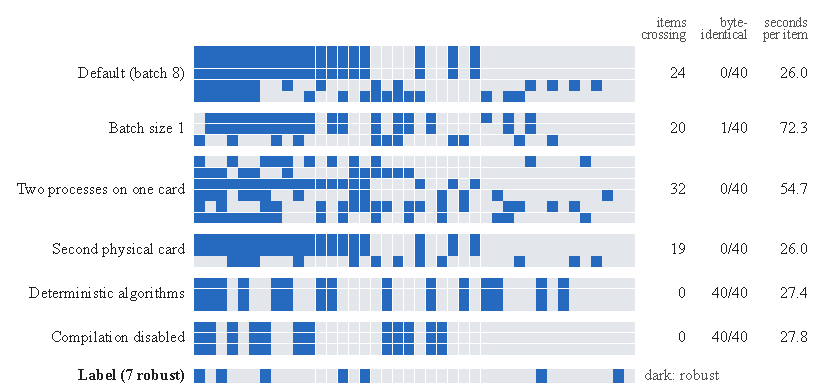
\includegraphics[width=\linewidth]{fig_rumore.pdf}
\caption{Predictions of the official pipeline for 40 preliminary public problems (columns) in 23 executions on DeepSeek (rows), by configuration; the last row is the label, dark cells are robust, and columns are sorted by how often they are predicted robust. At right: items whose prediction changes across the configuration's runs (more runs, more crossings), items whose generated text is byte-identical in all of them, and seconds per item.}
\label{fig:noise}
\end{figure}

\begin{table}[t]
\caption{Repeatability of the official pipeline on DeepSeek, 40 public problems, by configuration, in the order of Figure~\ref{fig:noise}. ``Crossings'': items whose prediction changes across the configuration's runs. ``Identical'': items whose generated text is byte-identical in all runs. Cost is runtime against the default configuration. Card 0 and card 1 are the two GPUs of the same machine. With two processes on one card, any five of its six runs give 29 to 31 crossings.}
\label{tab:reexec}
\centering
\small
\begin{tabular}{@{}lllllll@{}}
\toprule
\textbf{Configuration} & \textbf{Card} & \textbf{Runs} & \textbf{Crossings} & \textbf{Identical} & \textbf{Correct per run} & \textbf{Cost} \\
\midrule
Default (batch 8) & 0 & 5 & 24/40 & 0/40 & 24, 24, 24, 23, 24 & reference \\
Batch size 1 & 0 & 3 & 20/40 & 1/40 & 20, 21, 24 & +178\% \\
Two processes on one card & 0 & 6 & 32/40 & 0/40 & 24 to 28 & +110\% \\
Second physical card & 1 & 3 & 19/40 & 0/40 & 24, 24, 21 & +0\% \\
Deterministic algorithms & 0 & 3 & 0/40 & 40/40 & 24, 24, 24 & +5\% \\
Compilation disabled & 1 & 3 & 0/40 & 40/40 & 25, 25, 25 & +7\% \\
\bottomrule
\end{tabular}
\end{table}

\paragraph{Two candidate remedies.} Deterministic algorithms (PyTorch's, in warn-only mode, with deterministic cuDNN and a fixed cuBLAS workspace; Appendix~\ref{app:C}) and disabled compilation each made the generated text byte-identical in three sequential runs, at 5 to 7\% runtime cost. On card 0, the default configuration produced 24 crossings in five runs. Each remedy ran on one card where the default had produced crossings, each run in a new process, with no other process on that card. Three identical runs are weak evidence: the default configuration also gave three identical runs on card 0 before its fourth diverged, and five of its eight runs on the two cards shared one output. The two remedies produced different outputs, predicting 15 and 12 of the 40 problems robust, and because they ran on different cards we cannot tell whether the difference comes from the configuration or from the card. Neither gained more than one item (24 and 25 correct).

\paragraph{Distinct outputs.} The 23 executions fall into 14 distinct outputs, byte-identical within each. The same output appeared on both cards, and two runs launched in the same second on one card produced different outputs, so the output is not a property of the card alone; what selects it is not established. As only 7 of the 40 problems are robust and crossings largely cancel, accuracy moved much less than predictions: 21 to 24 correct in the default configuration on either card and 24 to 28 with two processes on one card, always below the 33 of the majority constant. An exploratory repetition of the official score extraction, whose third run ranks the 164 labeled problems at Spearman 0.24 against the first two, is in Appendix~\ref{app:C}.

\section{Regenerating the labels with our own protocol}\label{sec:labels}

\paragraph{Our labeling protocol.} We identified the organizers' perturbation families in the preliminary data (rephrase, rename, domain, distract, typos), regenerated them with gpt-oss-120b prompted with public examples, and gated each variant with gpt-oss-120b. An answer counts as correct when it matches gpt-oss-120b's answer on the original problem, because the preliminary data carry no answers; we did not check this key against the answers of the collections the problems come from. On the organizers' machine, with vLLM 0.28.0 [8] outside the official image, we labeled four models with two independent draws of variants (A and B, about 40 accepted variants per problem): 10 samples on the base problem and one per variant, at temperature 0.6, top-p 0.95 and at most 16,384 new tokens. Draw A's variants were also re-sampled with a new seed (A$'$). A label is robust when at least 6 of the 10 base samples are correct and every variant is answered correctly; unlike the earlier rule's conjunction, this requires the base problem to be solved.

A chain that reaches our cap is scored by the last boxed answer it contains, and counts as wrong without one; the organizers also count a response that reaches their limit without a parseable final answer as wrong [4]. Our protocol differs from the organizers' in perturbations, answer key, rule and sampling (one answer per variant, against 10 in the files behind most of their DeepSeek labels). Its decoding differs from the settings they publish, and its prompt may differ from the one behind their labels, which they have not stated.

\begin{table}[t]
\caption{Agreement of labels regenerated with our protocol: Cohen's kappa. The three columns for A and B treat variant chains that reached the 16,384-token cap in three ways: scored as in the protocol (by their last boxed answer, if any), dropped, or all counted as correct. The first of these columns and the A and A$'$ column give 95\% percentile bootstrap intervals over problems, and the script of Appendix~\ref{app:E} gives them for the other two. A problem has a label in a draw when it has at least one accepted variant (160 in A, 159 in B). Kappa between A and B uses the 159 problems labeled in both (150 for Qwen3.5-4B and 156 for DeepSeek when truncated chains are dropped), and between A and A$'$ 160. ``At cap'': percentage of variant chains that reached the cap in draws A and B. ``Robust'': percentage of problems labeled robust in draw A, as scored. The last column gives kappa of draw A with the organizers' preliminary DeepSeek labels: on the 138 published ones, and on the 160 that include 22 labels we derived (Section~\ref{sec:data}).}
\label{tab:label}
\centering
\small
\setlength{\tabcolsep}{3pt}
\begin{tabular}{@{}llllllll@{}}
\toprule
& & & \multicolumn{3}{l}{\textbf{A and B, truncated variant chains}} & & \\
\cmidrule(lr){4-6}
\textbf{Model} & \textbf{At cap} & \textbf{Robust} & \textbf{as scored} & \textbf{dropped} & \textbf{correct} & \textbf{A and A$'$} & \textbf{Organizers'} \\
\midrule
Skywork & 1.2, 1.5 & 74 & 0.44 [0.28, 0.59] & 0.39 & 0.39 & 0.79 [0.67, 0.89] & none \\
DeepSeek & 5.1, 6.1 & 39 & 0.41 [0.26, 0.55] & 0.35 & 0.36 & 0.46 [0.33, 0.59]$^{*}$ & 0.011; 0.025 \\
Olmo & 1.1, 0.9 & 68 & 0.38 [0.21, 0.54] & 0.39 & 0.39 & 0.65 [0.52, 0.78] & none \\
Qwen3.5-4B & 22.1, 29.2 & 9 & 0.18 [$-$0.06, 0.39] & 0.26 & 0.44 & not run & none \\
\bottomrule
\end{tabular}
\par\smallskip{\footnotesize $^{*}$On DeepSeek, A$'$ also received the answer-format line (end of this section), so this entry mixes seed and prompt.}
\end{table}

\paragraph{Results.} Under our protocol, two independent draws of variants give labels that agree at kappa 0.35 to 0.44 on Skywork, Olmo and DeepSeek, whether truncated variant chains are scored as in the protocol, dropped or all counted as correct (Table~\ref{tab:label}). On Qwen3.5-4B, 22 to 29\% of the variant chains reach the cap. Scoring these chains as in the protocol, dropping them or counting them all as correct gives agreement of 0.18, 0.26 and 0.44, and a robust share in draw A of 9\%, 83\% and 79\%. On Skywork, re-sampling the same variants with a new seed agrees far more than drawing new variants (0.79 against 0.44), so its label depends more on the variants than on the seed; on Olmo the gap is smaller (0.65 against 0.38), and on DeepSeek, where A$'$ also changed the prompt, it is 0.46 against 0.41.

Draw A's DeepSeek labels agree with the 138 labels the organizers published at kappa 0.011 [$-$0.13, 0.17], and with the 160 that include 22 of our derived labels at 0.025 [$-$0.12, 0.18]. Of the 36 problems with a published robust label, draw A calls 20 non-robust, and 4 of these change when truncated variants all count as correct. Of the 102 with a published non-robust label, draw A calls 44 robust. The reliability of the organizers' labels remains unmeasured. A retrospective calculation on the same saved answers with the main-phase threshold rule, applied as its pre-registration fixed it, with no filter on the base problem (Appendix~\ref{app:C}), gives test-retest point estimates between 0.34 and 0.56, below the pre-registered bar of 0.60, though three of the four intervals include it.

\paragraph{The prompt changes our labels.} In a first run with the bare problem text, later discarded, \mbox{Qwen3.5-4B} gave a final answer in the expected format in only 5 of its 1,640 base samples in draw A. With one instruction line requesting the format, 145 of 164 problems passed the base condition, against none. DeepSeek passed it on 147 of 164 with or without that line; its draws A and B ran without the line and A$'$ with it, and on the same variants its robust share moved from 39\% to 51\% of the 160 labeled problems, a change that mixes prompt and seed. Under our protocol, the label of Qwen3.5-4B therefore depends on the prompt. Whether this affects the organizers' labels is unknown: their baselines repository has a solve prompt that asks for an ANSWER line, but they have not said whether it was used for labeling (R3).

\section{The falsification campaign}\label{sec:campaign}

Table~\ref{tab:campaign} summarizes the campaign; Appendix~\ref{app:A} lists all 31 entries and explains three traps (rule T, the oracle H13, the duplicated pairs behind H2) and two pitfalls of the data. All entries use the preliminary data, except H16 to H18, which were scored on the 17 items of the warmup evaluation task.

\begin{table}[t]
\caption{The campaign in brief, in 19 of its 31 entries (Appendix~\ref{app:A} lists all). Ground truth is DeepSeek's and the preliminary pairs' unless stated; accuracy differences are in points against each pre-registration's baseline. H1, H7 and T count the 52 duplicated DeepSeek pairs twice; counted once, no verdict changes.}
\label{tab:campaign}
\centering
\small
\begin{tabular}{@{}L{5.5cm}L{1.9cm}L{5.6cm}@{}}
\toprule
\textbf{What we tested} & \textbf{Entries} & \textbf{Outcome} \\
\midrule
Text features; robustness as a property of the problem; labels, base accuracy and difficulty order across models & H1 to H5, H7 & rejected; H2 gained only when the duplicated pairs were counted twice \\
Official uncertainty features, logistic regression & H10 & 0.774 against a majority constant of 0.756, within the 0.692 $\pm$ 0.101 of the proposal [1] (method substituted) \\
Features cached for other models; per-target thresholds & H12, H13 & H12 rejected; the H13 ceiling withdrawn, $-$2.8 points when forced to rank \\
Our perturbation families, translation, self-consistency, the organizers' families regenerated (pilot), representation shift & H19, H22, H30 to H33 & rejected: kappa at most 0.02, AUROC at most 0.615 \\
Probes on DeepSeek's hidden states: ours and the organizers' published artifact & H36, H35 & survive their nulls; ours adds no detectable gain over length, and the artifact's score is probably in-sample \\
Trivial-robust rule, post hoc & T & a trap: +6.0 points on the preliminary pairs, +0.0 on \texttt{val-sample} \\
Identical bundles re-executed (warmup, 17 items) & H18 & noise confirmed: 11, 9, 11 and 11 correct \\
\bottomrule
\end{tabular}
\end{table}

\paragraph{Length and probes.} The character count of the problem alone orders the 164 DeepSeek labels at AUROC 0.704. Our logistic probe on DeepSeek's last-token hidden states, with layer and regularization chosen by inner cross-validation, reaches 0.710 out of fold with the original fold assignment. Over 20 other assignments, passed through the second-stage model below, it gives 0.57 to 0.76 (mean 0.69). Its scores correlate with length at Spearman +0.55, and residualized on log character count it gives 0.62. Its permutation null, rerun with 1{,}000 permutations of the whole nested procedure (the first version used 60, where 500 were pre-registered), gives $p = 0.002$. Restricted to the 138 published labels, these out-of-fold scores give 0.714 and length 0.733; retrained on those 138 alone with H36's procedure and seed, the probe gives 0.620. Combined with length in a second-stage model fitted on common outer folds, the probe changes AUROC over length alone by +0.005 on the 164 labels and by $-$0.010 on the 138 published ones (median bounds of the per-assignment 95\% intervals: $-$0.03 to 0.04, and $-$0.04 to 0.02): we detect no gain from adding the probe to length (Appendix~\ref{app:C}). This analysis replaces an earlier combination that leaked labels (Appendix~\ref{app:D}).

The organizers' published DeepSeek probe artifact orders the 164 DeepSeek labels at 0.739 with the aggregation we pre-registered and at 0.709 with its own, and at 0.62 and 0.57 residualized on log character count; its controls trained on shuffled labels give 0.68 at layer 31. The artifact does not record its training data; we infer that 137 of the 164 problems were among the public rows it was trained on, so these scores are probably largely in-sample. These length controls, which play the role of control tasks [7], were post hoc. Whether either probe reads anything beyond length that bears on robustness is not established. Apart from the three traps of Appendix~\ref{app:A}, no signal we scored by accuracy beats the majority constant by more than about one standard error on the preliminary labels, most of them DeepSeek's.

\section{Our entries}\label{sec:entries}

Our entry V8, pre-registered on 13 September, is the whole rule \texttt{return~[len(p)~>=~98 for~p~in~problems]}, with the threshold at the lower median of the 174 preliminary problems and the direction fixed on the preliminary pairs. On the original main-phase tasks it scored 11/21 and 10/19, like our entry v6 and the organizers' own entries. None of these beat the majority constant, which scores at least 11/21 and 10/19 on these tasks, and on so few items the ties do not show that length carries no signal (95\% Wilson intervals 0.32 to 0.72 and 0.32 to 0.73). On the 71 labeled rows of the official training set (revision of 17 September; 36 distinct problems), V8 differs from the all-robust constant on only 6 rows and is wrong on all 6 (46/71 against 52/71): too few to say what length is worth on official data. On the replacement tasks of 16 September, before and after the evaluation changed on 15 October [6], it predicted robust for every item (10/21 and 7/14), like an all-robust control. For the final test we nominated V8 (Codabench 1016713) and the constant (1016732), both on the Main track; our pre-registered predictions will be scored there (Appendix~\ref{app:B}).

\section{Recommendations}\label{sec:recs}

These rest mostly on DeepSeek and the preliminary data, and should be checked on the other models.
\begin{itemize}
\item \textbf{R1. Remove the variation between runs, and test the remedy:} on the same card with independent restarts, under load and across cards.
\item \textbf{R2. Repeat only where it decides something:} at the warmup's re-execution noise (a standard deviation of 1.0 item on 17, itself estimated from four runs), a one-item gap needs about eight runs per entry to reach two standard errors, so repeat only entries that run a model and sit near a prize boundary.
\item \textbf{R3. Say which prompt and decoding settings produced each released label file,} at least after the close.
\item \textbf{R4. Measure the label's reliability directly,} with two independent draws of variants labeled by the official process.
\item \textbf{R5. Show floors and noise on the leaderboard:} a row per constant predictor, the re-execution noise and binomial intervals.
\item \textbf{R6. Require a length control in white-box ablations.}
\item \textbf{R7. Remove the leaking field} \texttt{permutation\_type} from the aggregated datasets (Appendix~\ref{app:A}).
\end{itemize}

\paragraph{Code and data.} Our code, bundles, pre-registrations and outcome files are released at \href{https://github.com/Dan23RR/aimo-instrument}{\nolinkurl{github.com/Dan23RR/aimo-instrument}}. Its folder \texttt{reproduce/} recomputes the main tables from saved outputs and the six preliminary datasets, and the other numbers come from the dated records in \texttt{archive/} (Appendix~\ref{app:E}).

%%%%%% End of the main text: the six pages end here; the Limitations do not count %%%%%%
\label{fine-testo}

\section*{Limitations}

\begin{enumerate}[leftmargin=1.6em, itemsep=2pt, topsep=4pt, parsep=0pt]
\item \textbf{Preliminary data, not official data.} We did not repeat our label and probe analyses on the official training set, beyond the evaluation of V8 and a five-row check of our labels (Appendix~\ref{app:C}). Findings on label reliability and predictability may not generalize to the official evaluation setting.
\item \textbf{Our protocol, not the official one.} We did not regenerate labels with the organizers' published settings (100,000 tokens, temperature 1.0), with 10 answers per variant as in the files behind most DeepSeek labels, or on \texttt{train-main-v2}. The three treatments of truncated variant chains show how much our cap moves agreement between our draws; all three score base samples that reach the cap as the protocol does, and none of them reproduces longer decoding or a different temperature. Our low agreement with the organizers' labels is a fact about our process.
\item \textbf{One model.} We ran the probes, the re-execution study of Section~\ref{sec:reexec} and the comparisons of our regenerated labels with the organizers' preliminary labels only on DeepSeek.
\item \textbf{Re-execution.} We did not run the two candidate remedies on the same card, so card and configuration are confounded; we did not test either remedy under contention or on both cards, and we used 40 problems and one image.
\item \textbf{Records.} Some analyses rest on re-created scripts or dated records (Appendix~\ref{app:D}). Nothing here estimates performance on the final held-out problems.
\end{enumerate}

\section*{AI usage statement}

In this work, we used one generative AI tool, Claude (Anthropic), through Claude Code, for ideation, coding, analysis and writing. Ideation: it drafted the pre-registrations, including hypotheses, predictions and kill criteria, and searched and summarized the literature and the public records, including the organizers' Discord channels and the author's correspondence with them. Coding: it wrote the solution code of our bundles and the analysis and extraction scripts, ran them, and operated the organizers' virtual machine over SSH. Analysis: it computed and interpreted the results and ran automated adversarial reviews of hypotheses, drafts and code. Writing: it drafted the correspondence, this report and its revision after review.

It also made most of our Codabench uploads through the author's browser at the author's instruction. There were two exceptions: one resubmission (925822, 14 September), made without a specific instruction, and one submission that the author had not approved, sent in error and rejected before import (1016734, 28 October).

Language models were also components of our method: gpt-oss-120b generated and gated the perturbation variants and supplied the reference answers of Section~\ref{sec:labels}, and phi-4 translated problems for H22. The final decisions on the direction of the work, on the submissions (with the two exceptions above), on the nominations for the final test and on the claims of this report were the author's, and the author sent all correspondence personally. The author has reviewed all AI-assisted work and takes full responsibility for the final content of this report.

\begin{ack}
We thank Michal Štefánik, Róbert Belanec and the AIMO Interpretability team for the compute grant, a virtual machine with two GPUs, and for answering our questions; on 2 November they confirmed that the measurements taken on their machine may appear in this report. We also thank the three reviewers and the program chairs: two reviewers checked our analyses against the released code and data, and their checks corrected several of our claims. Other GPU time was rented on Modal and paid by the author or covered by Modal's platform credit. This work received no other funding, and the author has no competing interests.
\end{ack}

\section*{References}
{\small
[1] M. Štefánik, P. Mondorf, A. Waldis, Q. Liu, C. Yang, M. Spiegel, J. Kuchař, M. Kadlčík, A. Vawda-Oomerjee, C. Liu, S. Frieder, B. Plank, F. Barez and P. Stenetorp. AIMO Interpretability Challenge. CoRR, abs/2607.13899, 2026. doi:10.48550/arXiv.2607.13899.

[2] H. He and Thinking Machines Lab. Defeating Nondeterminism in LLM Inference. Thinking Machines Lab: Connectionism, 2025.

[3] J. Yuan, H. Li, X. Ding, W. Xie, Y.-J. Li, W. Zhao, K. Wan, J. Shi, X. Hu and Z. Liu. Understanding and Mitigating Numerical Sources of Nondeterminism in LLM Inference. NeurIPS 2025. arXiv:2506.09501.

[4] AIMO Interpretability Challenge website and FAQ. \url{https://aimo-interp.github.io} (accessed 28 October 2026), and its source repository aimo-interp/aimo-interp.github.io on GitHub.

[5] aimo-interp/getting-started and aimo-interp/baselines, GitHub repositories: README and issues \#6 and \#10 of getting-started; aimo-interp datasets on Hugging Face, including \texttt{train-main-v2} and \texttt{val-sample}.

[6] AIMO Interpretability Challenge Discord, \#announcements and \#qa: 5, 15 and 22 September, 9, 15, 16 and 20 October 2026.

[7] J. Hewitt and P. Liang. Designing and Interpreting Probes with Control Tasks. EMNLP-IJCNLP 2019.

[8] W. Kwon et al. Efficient Memory Management for Large Language Model Serving with PagedAttention. SOSP 2023.

[9] D. Hendrycks et al. Measuring Mathematical Problem Solving With the MATH Dataset. NeurIPS 2021 Datasets and Benchmarks Track. arXiv:2103.03874.
}

%%%%%% End of the references %%%%%%
\clearpage
\appendix
\raggedright

\section{The hypotheses, three traps and two pitfalls of the preliminary data}\label{app:A}

Section~\ref{sec:campaign} summarizes these entries. Unless stated, the ground truth is the 335 public pairs for H1 to H9 and T, the other models' preliminary labels for H12 to H15, the 17 items of the warmup evaluation set for H16 to H18, and DeepSeek's labels for the others. Validation that fits on some problems and tests on others is grouped by problem. The cross-model tests H7 and H12 to H15 hold out the model but not the problem, so part of them is in-sample; H7, H12, H14 and H15 were rejected anyway, and H13 is withdrawn. Numbers are accuracy points against each pre-registration's baseline unless they are kappa or AUROC.

{\small\setlength{\tabcolsep}{4pt}\renewcommand{\arraystretch}{1.2}
\begin{longtable}{L{1.1cm}L{3.9cm}L{5.6cm}L{2.0cm}}
\toprule
\textbf{ID} & \textbf{Hypothesis} & \textbf{Result} & \textbf{Verdict} \\
\midrule
\endfirsthead
\toprule
\textbf{ID} & \textbf{Hypothesis} & \textbf{Result} & \textbf{Verdict} \\
\midrule
\endhead
\bottomrule
\endlastfoot
H1 & The problem text predicts robustness (32 features) & 0.675 against 0.761, $-$8.7 ($-$7.4 with the duplicated pairs counted once) & rejected \\
H2 & Robustness is a property of the problem & with the 52 duplicated pairs counted once, z~=~0.88 and $-$1.3 against the per-model majority (bar 4.0); z~=~4.04 and +3.4 only when they are counted twice & rejected \\
H3 & One model's label predicts another's & $-$7.3 & rejected \\
H4 & One model's base accuracy predicts another's robustness & $-$11.8 & rejected \\
H5 & The difficulty order transfers across models & $-$25.4 & rejected \\
H6 & The same, with the oracle number of positives & $-$13.0 & ceiling (no kill criterion) \\
H7 & Base accuracy beats the prior on held-out models & $-$1.2 against the per-model majority that its pre-registration named (+0.0 against the global prior we used instead) & rejected \\
T & Robust if and only if base accuracy is below 0.05 (post hoc; see the traps below) & +6.0 on the 335 public pairs, +0.0 on \texttt{val-sample} & trap (no kill criterion) \\
H10 & The official uncertainty features reach the accuracy the proposal reports & 0.774 against a majority constant of 0.756, within 0.692 $\pm$ 0.101 [1]; a logistic regression on 13 of the 14 features of our own A100 re-implementation of the extraction (three of them constant), substituted for the official regressor & confirmed (method substituted, not declared at the time) \\
H11b & Length, saturation and trend features add signal & $-$1.8 and $-$2.5 & rejected \\
H12 & A cached model's uncertainty features predict other models & $-$16.5 & rejected \\
H13 & The same, with a threshold chosen per target & +7.3, from thresholds chosen on the scored items; $-$2.8 when forced to rank & withdrawn (no kill criterion) \\
H14, H15 & Calibration by the target's rate or by the global rate & $-$2.8 and $-$10.1 & rejected \\
H16 & Every model measured by itself beats the constant & 10/17 against 9/17 on one execution, inside the noise of H18 & survives, within noise \\
H17 & A gpt-oss threshold calibrated on \texttt{val-sample} beats H16 & 11/17, then 9, 11 and 11 on re-execution; 9/17 meets the kill criterion & not established \\
H18 & Identical bundles score differently across executions & 11, 9, 11 and 11 correct & confirmed (no kill criterion) \\
H19 & Our five mechanical perturbation families reproduce the organizers' preliminary label & accuracy 0.354 against 0.788, kappa 0.02 & rejected \\
H20 & A threshold tuned on our label transfers & 0.212 against 0.788 & rejected \\
H22 & Stability under translation reproduces the organizers' preliminary label & 0.507 against 0.740, kappa $-$0.10 & rejected \\
H23 & A threshold tuned on it transfers & +0.0 & rejected \\
H29 & Representation-distance features are repeatable (gate; written plan, not a frozen pre-registration) & ICC 0.997 to 0.999, from the dated outcome file & passes \\
H30 & The representation shift under perturbation predicts the label (written plan) & AUROC 0.615, below the kill threshold of 0.655; character count 0.704 (0.705 in E11's own computation) & rejected \\
H31 & The direction of that shift predicts the label (written plan) & AUROC 0.555 & rejected \\
H32 & The organizers' families, regenerated (pilot), reproduce their label & kappa $-$0.001 on four families, $-$0.030 with all five & rejected \\
H33 & Self-consistency over 8 samples predicts the label & AUROC 0.502 & rejected \\
H35 & The organizers' published probe artifact orders the 164 DeepSeek labels & 0.739 under the pre-registered aggregation and 0.709 under its own; 0.62 and 0.57 once residualized on log character count; its shuffled-label controls give 0.68 at layer 31 & survives its null; probably in-sample, not separated from length \\
H36 & Our linear probe, nested cross-validation, orders the 164 DeepSeek labels & 0.710 out of fold, above its permutation null, and 0.62 once residualized on log character count; 0.714 against 0.733 for length on the 138 published labels (Appendix~\ref{app:C}) & survives its null; no detectable gain over length \\
E13b-1 & Under the main-phase rule our regenerated label is test-retest reliable (kappa at least 0.60 on 3 of 4 models) & 0.34 to 0.56, retrospective (Appendix~\ref{app:C}) & rejected \\
E13b-2 & Under the main-phase rule it agrees with DeepSeek labels we computed with that rule from the preliminary data (kappa at least 0.40) & 0.02 [$-$0.09, 0.13] & rejected \\
E13b-3 & The labeling rule drives the instability of our regenerated labels & a gain of at least 0.15 on 2 of 4 models, where 3 were required; 0 of 4 on common problems & rejected \\
\end{longtable}
}

Not in the table are H8, H9, H21, H24 and H25 to H28. H8 is an oracle ceiling: 0.774, +1.8 points against the global constant and +0.4 against the per-model majority, with the duplicated pairs counted once. The outcome of H9 became rule T. H21 and H24 needed H19 and H20, and H22 and H23, to survive, so they were not run. H25 to H28 are entries of the E11 plan that its outcome file does not report under these identifiers. H25 is an anomaly of our own re-implementation of the extraction, found before the plan. H26 is the list field of the first pitfall below. H27 is a label-noise ceiling, which the plan itself closed with a resampling estimate instead of a test. H28 is the text-only baseline, which became character count (Appendix~\ref{app:D}). Three further E11 tests were not run (Appendix~\ref{app:D}). V4, an entry submitted once against its own pre-registered rule, is in Appendix~\ref{app:D}.

\paragraph{Three traps.} Rule T gains six points on the public pairs and nothing on \texttt{val-sample}, because the trivially robust items (base accuracy 0, robust under the conjunction) are absent there. The oracle H13 chose each target's threshold among all cut points on the very items it was scored on; forced to rank the items and to predict the true number of positives, it gave $-$2.8. H2 owed its survival to one measurement published under two model names and counted twice; counted once, its z falls from 4.04 to 0.88.

\paragraph{Two pitfalls of the preliminary data.} In the three aggregated datasets, the field \texttt{permutation\_type} is a list if and only if the item is robust, because the aggregation merges all perturbation types into one row for robust items and keeps one row per retained type otherwise, usually a single type. The rule ``robust if the field is a list'' reproduces all 223 labeled rows of the three datasets, and the field does not exist at inference (recommendation R7). And 20 of the 80 robust pairs among the 335 have base accuracy 0. None of them carries a published label, so they are robust only under the conjunction we used to derive their labels, while \texttt{val-sample} has no labeled pair with base accuracy below 0.05.

\section{Pre-registered predictions for the final evaluation}\label{app:B}

P1 was written on 7 September 2026, P-V8 on 13 September and P-V8b on 21 September. They are translated from the dated files and shortened. We omit the runtime predictions (under 60 seconds), which we could not score because the bundles log no runtime. A second prediction written with P1 on 7 September concerns another participant's final score and is not reported here.

\begin{itemize}
\item \textbf{P1.} The top-ranked entry's accuracy on the final held-out problems will lie within two binomial standard errors of that set's majority-class constant.
\item \textbf{P-V8.} If the organizers had neutralized length, V8 would score between 0.45 and 0.55 on both tracks (stated beforehand as the most likely outcome); if they had not, and the set was balanced, about 0.66. Observed on the original tasks: 0.52 and 0.53, inside the first band; on 21 and 19 items, however, 0.66 lies inside the 95\% intervals of both scores, so the scores do not exclude the second.
\item \textbf{P-V8b}, on the replacement tasks: the same bundles work with the new ingestion and score 6 to 15 of 21 and 4 to 10 of 14. Observed: coverage 1.0, no invalid predictions, 10/21 and 7/14, inside the bands but degenerately, since the rule predicted robust for every item.
\end{itemize}

\section{Protocols, run manifest and recalculations}\label{app:C}

\paragraph{Hardware and software.} The generation runs used the organizers' virtual machine with two NVIDIA RTX PRO 6000 Blackwell Server Edition GPUs (96 GB each), the evaluation workers' model, from 8 September 2026. Each run used one GPU; the Olmo-3-7B-Think A$'$ labels combine two runs, one on each card (below).
\begin{itemize}
\item \textbf{Official runtime image.} Section~\ref{sec:reexec} and the official score channel (E16) ran inside it: {\footnotesize\path{ghcr.io/aimo-interp/aimo-codabench-runtime:torch2.12.1-cuda13.2-cudnn9-transformers5.13.0-sklearn1.8.0-kernels0.15.2}}, digest {\footnotesize\path{sha256:fb4dab6343de7ce022ddd7906493f9ced16ff9008d497326a781d1e5adc8207a}}. They used the official extraction and regressor as shipped in our bundles: greedy decoding, at most 4,096 new tokens, static cache, batch 8.
\item \textbf{Labeling environment.} Section~\ref{sec:labels} ran with vLLM 0.28.0, torch 2.13.0 and transformers 5.16.1 (driver 610.57.04 with CUDA 13.3 on the machine, CUDA 13.0 runtime libraries in the environment) in a separate environment on the same machine; \texttt{vm\_backup/AMBIENTE\_VM\_2026-09-17.txt} lists every package.
\item \textbf{Model revisions.} Hugging Face snapshot hashes: Qwen3.5-4B \texttt{851bf6e8}, Skywork-OR1-Math-7B \texttt{fcef970f}, Olmo-3-7B-Think \texttt{d97e442d}, DeepSeek-R1-0528-Qwen3-8B \texttt{6e8885a6}, gpt-oss-120b \texttt{b5c939de}. The full hashes are in the run logs.
\item \textbf{Analyses.} They ran on CPU: E13's analysis and E15's evaluation, up to 14 September, on the virtual machine (Python 3.12, NumPy 2.3.5, scikit-learn 1.9.1), the others on the author's computer (Python 3.11.12, NumPy 2.4.4 and scikit-learn 1.8.0, as recorded for the runs of September and November). The release pins every output by SHA-256 in \texttt{MANIFEST.tsv}.
\end{itemize}

\needspace{8\baselineskip}
\paragraph{Run manifest.}
\begin{itemize}
\item \textbf{Where they ran.} The scripts in \texttt{vm/} written up to 14 September (setup, generation, extraction, E13's analysis and E15's evaluation), after which the machine stayed idle, and the clean-up script of 17 September ran on the virtual machine; the later ones ran on the author's computer.
\item \textbf{Outputs} are in \texttt{vm\_risultati/} unless the table gives another path.
\item \textbf{GPU-hours} are times from the logs (\texttt{reproduce/compute\_hours.py}). They include model loading except for the E13 labels, a difference under 1\%.
\end{itemize}

{\small\setlength{\tabcolsep}{4pt}
\begin{longtable}{L{2.4cm}L{3.2cm}L{2.2cm}>{\raggedright\arraybackslash\footnotesize}p{4.8cm}}
\toprule
\textbf{Run} & \textbf{Where it ran} & \textbf{GPU-hours} & \textbf{Outputs} \\
\midrule
\endfirsthead
\toprule
\textbf{Run} & \textbf{Where it ran} & \textbf{GPU-hours} & \textbf{Outputs} \\
\midrule
\endhead
\bottomrule
\endlastfoot
E13 variants & virtual machine & 1.15 and 1.20 & \path{e13/varianti_D1.parquet}, \path{e13/varianti_D2.parquet} \\
E13 labels & virtual machine, one queue per card & 64.4, in the logs of the 11 runs of Table~\ref{tab:label} & \path{e13/etich_*.parquet} \\
E13b, main-phase rule & author's computer & CPU only & \path{e13b_regola_nuova_2026-09-21.txt} \\
E14 re-execution & virtual machine, official image & 8.4 & \path{e14/out/*.jsonl}, \path{e14/log/} \\
E15 extraction & virtual machine & under 0.1 & \path{vm_backup/estratto/work/aimo/e15/hs_*.npz} \\
E15 probes & the virtual machine's CPU on 14 September, then the author's computer & CPU only & \path{e15_*}, \path{e15r/}, \path{vm_backup/estratto/work/aimo/e15_valuta.log} \\
E16 score channel & virtual machine, official image & 5.9 & \path{e16_*.jsonl}, \path{e16nodet/} \\
\end{longtable}
}

\paragraph{Commands.} Script paths are relative to \texttt{archive/}, the working folder of the repository. The scripts in \texttt{vm/} that ran on the virtual machine use paths under \texttt{/work/aimo}. \texttt{M} stands for the model, and in E14 \texttt{C}, \texttt{r}, \texttt{g} and \texttt{t} for the configuration, repetition, card and process tag.
\begin{itemize}
\item \textbf{E13 variants.} \texttt{vm/e13\_varianti.py -{}-draw~D1 -{}-seed~20260913 -{}-n~164 -{}-k~10}, and \texttt{-{}-draw~D2 -{}-seed~20260914}. The model gpt-oss-120b generates, solves and gates the variants (prompts below).
\item \textbf{E13 labels.} DeepSeek A and B ran an earlier version of \texttt{e13\_etichetta.py} that sent the bare problem text (now \texttt{-{}-prompt~nudo}); every other run behind Table~\ref{tab:label}, DeepSeek A$'$ included, used the explicit prompt. Draw A: \texttt{vm/e13\_etichetta.py -{}-model~M -{}-cond~A -{}-draw~D1 -{}-seed~20260921 -{}-prompt~esplicito}; B: \texttt{-{}-cond~B -{}-draw~D2 -{}-seed~20260922}; A$'$: \texttt{-{}-cond~Ap -{}-draw~D1 -{}-seed~20260923}. \texttt{vm/e13\_coda.sh} launched one queue per card (its logs are in \path{vm_backup/estratto/work/aimo/}); the card 0 queue ran an earlier version that passed no \texttt{-{}-prompt} flag, so DeepSeek A$'$ got the default of \texttt{e13\_etichetta.py}, the explicit prompt.
\item \textbf{E13b.} \texttt{vm/e13b\_regola\_nuova.py}, on the saved E13 answers; retrospective (below).
\item \textbf{E14.} \texttt{vm/e14\_all.sh 40 "C0 C1 C2 C3"} and \texttt{vm/e14\_extra.sh 1 "C5 C4"}. Each run is \texttt{e14\_run.py -{}-cond~C -{}-rep~r -{}-gpu~g -{}-tag~t -{}-n~40} inside the official image: 23 runs on DeepSeek. In the 8.4 GPU-hours the two processes of each contention pair, which shared one GPU, count once (20 runs).
\item \textbf{E15 extraction.} \texttt{vm/e15\_estrai.py -{}-model~deepseek-ai/DeepSeek-R1-0528-Qwen3-8B}, with and without the official system prompt: one forward pass per problem, last input token, all 37 hidden-state indices, at most 2,048 tokens.
\item \textbf{E15 probes.} \texttt{vm/e15\_valuta.py} ran H35, H36 and the first null (60 permutations) on 14 September, on the virtual machine's CPU; its log is \path{vm_backup/estratto/work/aimo/e15_valuta.log}. The file \path{vm_risultati/e15_valuta_2026-09-14.txt} is a later run of that day, by the file times in \path{vm_backup/MANIFEST_backup_aimo_2026-09-17.txt}, that stopped with an error at the null. H35's null is the 95th percentile, 0.602, of the AUROC of 20{,}000 random scores on the same labels, in either orientation. \texttt{vm/e15\_null\_nidificato.py} reran that null on 23 September with both grids of $C$, on the author's computer. E15-R (below) is \texttt{vm/e15r\_ricalcolo.py}, given an output folder and a number of worker processes (5 on the author's computer, 14.5 hours); its outputs are in \texttt{vm\_risultati/e15r}, and since it appends to existing files, a rerun needs a new folder. H35 needs the organizers' artifact \texttt{probe\_artifact.pkl} (hash below), which we do not redistribute.
\item \textbf{E16.} \texttt{vm/e16\_all.sh} and \texttt{vm/e16\_nodet.sh}, in the official image. Of the variables that \texttt{e16\_all.sh} sets, only the cuBLAS workspace variable reaches the extraction; \texttt{e16\_nodet.sh} sets neither.
\end{itemize}

The organizers' artifact used by H35 has SHA-256 {\footnotesize\texttt{8607478c7408922a6490adb7bda34d6a7d95403b7aa62f80dd3f2649139ccdeb}}. The listed logs total 82.8 GPU-hours. Not in the table:
\begin{itemize}
\item two complete runs of Qwen3.5-4B with the bare prompt (about 13 GPU-hours, no released log);
\item a partial run of Qwen3.5-4B A$'$ with the bare prompt (1.7 GPU-hours, included in the 82.8), discarded with them;
\item a run of Olmo-3-7B-Think A$'$ on card 1 (11.0 GPU-hours, 07:19 to 18:21 UTC on 10 September, from its queue log). Card 0 reached the same condition at 14:20, resumed from its partial file with 96 of the 164 problems done and finished the other 68, so the reported A$'$ labels come from both cards.
\end{itemize}
With these, the virtual machine ran about 107 GPU-hours, plus short smoke and feasibility tests. Our earlier runs on Modal used about 12 to 13 GPU-hours, mostly on A100 GPUs, as documented in their dated outcome files: the feature extraction behind H10, its pilot, and E9 to E12.

\paragraph{What can be recomputed.}
\begin{itemize}
\item \textbf{From saved outputs.} The scripts in \texttt{reproduce/} (Appendix~\ref{app:E}), which also read the six preliminary datasets; the other numbers come from the dated records in \texttt{archive/}.
\item \textbf{On a CPU, from the released hidden states.} Our probe (H36) and E15-R can be rerun end to end. H35 also needs the organizers' artifact.
\item \textbf{Only with the original GPUs and models.} The generation runs.
\end{itemize}

\paragraph{Re-execution configurations (Section~\ref{sec:reexec}).}
\begin{itemize}
\item \textbf{C0, default:} batch 8, on card 0, five runs.
\item \textbf{C1, batch size 1.}
\item \textbf{C2, deterministic algorithms:} \texttt{torch.use\_deterministic\_algorithms(True, warn\_only=True)}, \texttt{cudnn.deterministic = True}, \texttt{cudnn.benchmark = False} and \texttt{CUBLAS\_WORKSPACE\_CONFIG=:4096:8}.
\item \textbf{C3, contention:} two identical processes at the same time on card 0, three pairs.
\item \textbf{C4, second card:} the default on card 1.
\item \textbf{C5, compilation disabled:} \texttt{TORCH\_COMPILE\_DISABLE=1}, on card 1.
\end{itemize}
Runs within a configuration were sequential, each a new process. During these runs the other card was running another of our jobs. Two pre-registered predictions failed:
\begin{itemize}
\item batch size 1 did not make generation more repeatable: three runs gave three different outputs;
\item disabled compilation was predicted to land in one of the default outputs; it was byte-identical across its runs, but in an output of its own.
\end{itemize}
\texttt{reproduce/reexecution\_table.py} recomputes Table~\ref{tab:reexec} and the numbers of Figure~\ref{fig:noise}, and lists the 14 distinct outputs.

\paragraph{Variants and labels (Section~\ref{sec:labels}).}
\begin{itemize}
\item \textbf{Few-shot pool.} The generator saw five public examples of each family, drawn from a pool of 621 public examples (original, perturbed) over the five families. The texts are the organizers' and are not redistributed. \texttt{vm\_risultati/e13/fewshot\_pool\_ids.json} lists each example's problem identifier and SHA-256 hashes, and \texttt{reproduce/fewshot\_pool.py} rebuilds the pool from the downloaded preliminary datasets (verified on 23 November 2026: 621 of 621, byte-identical).
\item \textbf{Drawing the examples.} For draw seed $s$, problem $p$ and family $f$, the five examples are \texttt{random.Random("s|p|f").sample(pool[f] without p, 5)}.
\item \textbf{Generator.} gpt-oss-120b at low reasoning effort, temperature 1.0, top-p 1.0, at most 4,096 tokens, one request per problem and family, asking for 10 variants.
\item \textbf{Gate and reference answers.} gpt-oss-120b at medium effort, temperature 1.0, at most 8,192 tokens, solves the original and each variant. A variant is accepted if its text differs from the original, the length ratio lies between 0.7 and 4.0, and the solver's answer is unchanged. The solver's answer on the original is the reference answer.
\item \textbf{Labeling.}
  \begin{itemize}
  \item \textbf{Prompt.} Each model receives the instruction line (the second block below) followed by the problem, except DeepSeek in A and B, which received the bare text.
  \item \textbf{Sampling.} Temperature 0.6, top-p 0.95, at most 16,384 new tokens (raised from 8,192 before execution, after a test in which 2 of 3 problems saturated 8,192). There are 10 samples on the base problem and one per accepted variant.
  \item \textbf{Scoring.} A chain is scored by the last boxed answer it contains. Without one, including when it was cut at the cap, it counts as wrong.
  \end{itemize}
\end{itemize}

{\footnotesize
Generator prompt:
\begin{quote}\ttfamily
You create variants of mathematics competition problems for a robustness benchmark. Perturbation type: <family>. <family instruction> The variant must be a complete, self-contained problem with exactly the same final answer as the original. Do not solve the problem. Do not add hints or solutions. Here are 5 examples of this perturbation type: Example 1 Original: <public original> Variant: <public variant> (four more examples) Now write 10 different variants of the following problem. Make them genuinely different from each other. Output each variant between <variant> and </variant> tags, and nothing else. Original: <problem>
\end{quote}
Instruction line of the labeling prompt, also used by the solver of the gate:
\begin{quote}\ttfamily
Solve the following problem. Reason step by step, then give only the final answer inside \textbackslash{}boxed\{\}.
\end{quote}
}
The five family instructions, verbatim:
\begin{itemize}
\item rephrase: ``Rewrite the problem in different words while preserving exactly its mathematical content and its final answer.''
\item rename: ``Rename the variables, people, objects or entities in the problem while preserving its mathematical structure and its final answer.''
\item domain: ``Transfer the problem to a different real-world surface domain (a different story, setting and objects) while preserving exactly the same mathematical structure and the same final answer.''
\item distract: ``Insert irrelevant but plausible additional information (extra facts, numbers or context) that does not change the problem or its final answer.''
\item typos: ``Introduce harmless typographical or formatting noise (misspellings, spacing, punctuation, capitalisation) without changing the meaning of the problem or its final answer.''
\end{itemize}

\paragraph{The main-phase rule, retrospectively (E13b).} PREREG\_E13b was written on 21 September, before any calculation under the main-phase rule but after the E13 answers had been measured, so the calculation is retrospective.
\begin{itemize}
\item \textbf{The rule.} On the saved answers, a problem is robust if the largest drop in accuracy across families is at most 0.10 and non-robust if it is at least 0.25; problems in between get no label.
\item \textbf{No base filter.} As pre-registered, the primary calculation has no filter on the base problem, so a problem the model never solves counts as robust when no family lowers its accuracy.
\item \textbf{Test-retest, primary.} Kappa between A and B is 0.34 [0.13, 0.53] on 86 problems (Qwen3.5-4B), 0.49 [0.17, 0.76] on 132 (Skywork), 0.41 [0.09, 0.69] on 133 (Olmo) and 0.56 [0.36, 0.73] on 100 (DeepSeek). Because 58 to 95\% of the problems are labeled robust, kappa stays low even where raw agreement is high.
\item \textbf{Test-retest, secondary (S1).} On problems with at least 5 of 10 correct base samples in both draws, kappa is 0.31, 0.52, 0.40 and 0.55.
\item \textbf{Against the organizers.} Against DeepSeek labels that we computed with the same rule from the accuracy drops published in the preliminary data: 0.02 [$-$0.09, 0.13] on 133 problems.
\item \textbf{Against \texttt{train-main-v2}.} On its five labeled rows that fall on our problems and models, our labels agree with the official ones on 2 (draw A, one undefined) and 3 (draw B); five rows are too few to read.
\item \textbf{Truncated chains} are scored as in the protocol here too.
\end{itemize}

\paragraph{Subsampling (E13).} Subsampling DeepSeek's variants from 2 to 40 per problem leaves the mean kappa between A and B between 0.36 and 0.47, with no upward trend: more variants per problem do not make our labels more repeatable.

\paragraph{The official score channel (E16, exploratory).} We extracted the official regressor score on DeepSeek three times for the 174 public problems with the same code and image; this measurement was not pre-registered. The first run set the cuBLAS workspace variable and gave the same scores as the second, run without it, on all 174 problems. The second and third correlate at Spearman 0.24 over the 164 labeled problems. They give AUROC 0.487 and 0.602 in the regressor's own orientation; the paired bootstrap 95\% interval of their difference, $-$0.015 to 0.246, includes zero. The ranking of the problems was not reproduced in one of two repetitions; this does not show that the signal itself changes. As 137 of the 164 problems are in the regressor's training set, this concerns the stability of its inputs, not new problems. The 5.9 GPU-hours of the manifest also include one extraction each on Qwen3.5-4B, Skywork and Olmo, which this report does not use, and a failed start on gpt-oss-120b.

\paragraph{E15-R: the probe recalculated after review.} The procedure was fixed in \texttt{vm/e15r\_ricalcolo.py} before it ran, in a run started on 23 November 2026. It uses the same hidden states, labels and nested cross-validation as H36: layers 1 to 36, $C$ in \{0.001, 0.01, 0.1, 1\}, 5 outer and 4 inner folds.
\begin{itemize}
\item \textbf{Combination with length.}
  \begin{itemize}
  \item There are 20 fold assignments on the 164 labels and 10 on the 138 published ones.
  \item The probe's scores for the outer training problems come from a nested cross-validation inside them. Its score for each outer test problem comes from a probe selected and fitted on the outer training problems.
  \item A second-stage logistic regression on log character count, on the probe score, or on both, is fitted on the outer training problems and scored on the outer test problems.
  \item The 95\% interval of the gain of ``both'' over length is a paired bootstrap over problems (2,000 resamples) for each assignment; we report the median of its bounds.
  \end{itemize}
\item \textbf{Retraining.} The nested probe is retrained on the 138 published labels alone.
\item \textbf{Permutation null.} The null of H36 is extended from 60 to 1,000 permutations of the whole nested procedure, with the seeds of the first 60 unchanged.
\end{itemize}
We fixed the decision rule before the run: if the interval of the gain includes zero, the probe adds nothing measurable to length.

\begin{center}
\small
\begin{tabular}{@{}lllll@{}}
\toprule
\textbf{Labels} & \textbf{Length} & \textbf{Probe} & \textbf{Both} & \textbf{Gain of both over length} \\
\midrule
164 (20 assignments) & 0.696 & 0.692 & 0.701 & +0.005 [$-$0.03, 0.04] \\
138 published (10 assignments) & 0.729 & 0.644 & 0.720 & $-$0.010 [$-$0.04, 0.02] \\
\bottomrule
\end{tabular}
\end{center}
Values are means over the assignments. Length and probe here are the second-stage models, cross-validated and pooled over folds, so they differ slightly from the raw values of Section~\ref{sec:campaign} (0.704 and 0.733 for character count). On the 164 labels the gain ranges from $-$0.024 to +0.023 over the 20 assignments, and its interval excludes zero in 1 of them; the probe's second-stage model alone ranges from 0.57 to 0.76. The inner cross-validation chose hidden-state index 4 in 66 of the 100 outer folds. On the 138 published labels the gain ranges from $-$0.026 to +0.012 over the 10 assignments. With H36's procedure and random seed, the probe retrained on the 138 published labels alone gives AUROC 0.620, against 0.733 for character count; the probe's second-stage model of the table ranges from 0.59 to 0.71 over its 10 assignments.

The null with 1{,}000 permutations has mean 0.4975 and 95th percentile 0.6032; 1 permutation reaches the observed 0.710 ($p = 0.002$). Its first 60 permutations reproduce the null of 23 September (mean 0.4890, 95th percentile 0.5700) to the last digit. The run stopped after 925 permutations, when the computer restarted; \texttt{vm/e15r\_riprendi.py} computed the other 75 with the same permutations and seeds.

\section{Withdrawn claims, deviations and records}\label{app:D}

\paragraph{Claims withdrawn after review.}
\begin{itemize}
\item \textbf{A bound on latent agreement.} We had corrected the kappa of 0.025 with the organizers' DeepSeek labels for our own noise and quoted about 0.27 as an upper bound on latent agreement. That needs a measurement-error model for binary labels that we had not justified.
\item \textbf{The combination of probe and length.} Its earlier second-stage cross-validation reused probe scores computed on other folds, so some training scores depended on test labels. Its numbers (0.696 for length, 0.697 for the probe, 0.714 for both) are replaced by E15-R (Appendix~\ref{app:C}).
\item \textbf{Re-execution.} We no longer infer that the output of a run is fixed when the process starts.
\item \textbf{A simulation.} A plug-in simulation of the organizers' labeling process, which we had reported as overstating test-retest agreement by about 0.4, is no longer reported. It was a model of their process, not a measurement of it.
\end{itemize}
The other changes after review are listed in the repository README.

\paragraph{Deviations from the pre-registrations.} Each pre-registration is dated before execution, and the deviations below are also recorded as notes in those files.
\begin{itemize}
\item \textbf{Not pre-registered.} E5 is documented only in its outcome file. E11 ran from a written plan without the frozen pre-registration it called for. E16 was not pre-registered, although we had told the organizers that every experiment on their machine would be.
\item \textbf{E4.} H7 was compared with the global prior of the training models instead of the pre-registered per-model majority, against which it scores $-$1.2 points.
\item \textbf{E6.} H10 was run as a logistic regression on 13 of the 14 features in place of the pre-registered regressor and threshold, and this was not declared at the time.
\item \textbf{E11.}
  \begin{itemize}
  \item Three planned primary tests were not run.
  \item A Holm correction was planned and not applied, and H30 would fail it.
  \item The confirmation set was not held out.
  \item AUROCs were computed on raw scores, with the orientation chosen on the data.
  \item Only one of the three planned layer depths (0.80, the primary one) was extracted.
  \item The six-feature text baseline of H28 was replaced by character count alone, and the two reference analyses the plan required next to every AUROC were not computed.
  \end{itemize}
\item \textbf{E13.}
  \begin{itemize}
  \item gpt-oss-120b was pre-registered for labeling and not labeled.
  \item DeepSeek's A$'$ received the answer-format line through a queueing error.
  \item The pre-registered table that mapped outcomes to readings was not followed, because it assumed our regeneration reproduces the organizers' process.
  \item The subsampling curve varied the variants per problem, where the design varied them per family.
  \item The token cap was raised from 8,192 to 16,384 before execution.
  \end{itemize}
\item \textbf{E13b.} It was written after the E13 answers had been measured (Appendix~\ref{app:C}).
\item \textbf{E14.} Its fourth measure, the repeatability (ICC) of the 14 official features, was not computed, and two of its predictions failed (Appendix~\ref{app:C}).
\item \textbf{E15.}
  \begin{itemize}
  \item It predicted that both probes would fail their nulls; both survived.
  \item H36's nested null was pre-registered with 500 permutations and the full grid of $C$. The first run (14 September) used 60 permutations and two values of $C$. It was rerun with the full grid on 23 September, and extended to 1{,}000 permutations in a run started on 23 November.
  \item The Holm correction over the two primaries was not computed.
  \item The length controls of H35 and H36 were post hoc.
  \end{itemize}
\item \textbf{V4.} The allocation entry (909843) predicted robust on the 9 warmup items of gpt-oss-120b. It combined three numbers: the share of robust items implied by public leaderboard scores of constant entries, the count of gpt-oss-120b items read from the log of our warmup submission 907310, and that model's higher robust rate in the preliminary datasets (0.40 against 0.24). Our compliance review found that without the first two, which describe the evaluation set, it reduces to the entry it modified. Its pre-registration said it would not be sent if that review refuted it; the review did, and the author submitted it once anyway, as a measurement kept off the leaderboard. It tied the entry it modified.
\end{itemize}

\paragraph{Records.} Several analyses were first run from scripts that were not saved, and were re-created and saved later. The two length-control scripts of E15 and the rerun of its null were re-created on 23 September, each checked against the logged values before use. A few figures rest only on a dated record, not on a saved per-item output: H29's repeatability, the GPU-hours on Modal, and V8's predictions on the replacement and current tasks, which come from counts its container logged.

\paragraph{Earlier corrections.} Between our first drafts and the submitted version we corrected 54 of our own statements. They are listed, with what each changed, in \texttt{CORRECTIONS.md} in the repository, and every number in this report already includes them. The main text cites English entry points (\texttt{reproduce/}); the commands of the run manifest keep the original script names, which the dated pre-registrations cite.

\section{Data, assets, release and submissions}\label{app:E}

\paragraph{Data.}
\begin{itemize}
\item \textbf{Preliminary datasets.} The six datasets published by the organizers under \texttt{aimo-interp} on Hugging Face before the main phase: \texttt{val-sample}, \texttt{augmented-sample-math}, \texttt{augmented-sample-math-full-filtered}, \texttt{augmented-sample-math-agg-filtered}, \texttt{aimo-interp-challenge-sample-full} and \texttt{augmented-sample-math-agg}. Their cards state no license. Their problems come from the MATH dataset [9] and from the AIMO 2025 reference problems, as their \texttt{dataset\_id} field records.
\item \textbf{Official training set.} \texttt{train-main-v2} at revision 23791d9 of 17 September 2026 (82 rows, 71 labeled; the organizers extended it to 94 rows on 15 October). Its card states the license as ``other''.
\item \textbf{Downloading.} \texttt{dati.py} downloads the six preliminary datasets; we do not redistribute copies of the organizers' datasets. Our analyses used the files below. Their SHA-256 values begin as follows, and \texttt{reproduce/README.md} gives them in full.

\smallskip
{\small\begin{tabular}{@{}ll@{}}
\texttt{aimo-interp-challenge-sample-full} & \texttt{b8a57039} \\
\texttt{val-sample} & \texttt{afae22a0} \\
\texttt{augmented-sample-math-agg} & \texttt{3d168c29} \\
\texttt{augmented-sample-math-agg-filtered} & \texttt{a96bf90d} \\
\texttt{augmented-sample-math} & \texttt{991b74c0} \\
\texttt{augmented-sample-math-full-filtered} & \texttt{1b62215f} \\
\end{tabular}}
\end{itemize}

\paragraph{Models and code.} The models used, with their licenses:
\begin{itemize}
\item gpt-oss-120b (OpenAI, Apache-2.0);
\item Olmo-3-7B-Think, and Olmo-3-7B-Instruct of the warmup evaluation set (Allen Institute for AI, Apache-2.0);
\item DeepSeek-R1-0528-Qwen3-8B (DeepSeek, MIT);
\item Qwen3.5-4B (Qwen, Apache-2.0);
\item Skywork-OR1-Math-7B (Skywork; no license stated on its card);
\item phi-4 (Microsoft, MIT), for the translations of H22;
\item gemma-3-27b-it (Google, Gemma Terms of Use), loaded by our warmup entries for H16 to H18.
\end{itemize}
From the organizers we used the evaluation harness, the official uncertainty-feature extraction with its DeepSeek regressor, and the DeepSeek probe artifact with its inference code (\texttt{aimo-interp/getting-started}, which states no license); from \texttt{aimo-interp/baselines} (Apache-2.0) we used three files [5]. vLLM [8] (Apache-2.0) ran the generation, gating and labeling of Section~\ref{sec:labels}.

\paragraph{Release.} In \href{https://github.com/Dan23RR/aimo-instrument}{\nolinkurl{github.com/Dan23RR/aimo-instrument}}, the folder \texttt{archive/} keeps the layout of our working folder, with the dated records gathered in \texttt{archive/records/}. The file paths cited in this report are relative to \texttt{archive/}, except \texttt{reproduce/}, \texttt{MANIFEST.tsv} and \texttt{CORRECTIONS.md}, which sit at the top of the repository next to \texttt{paper/}, this report's sources.
\begin{itemize}
\item \textbf{Contents.} The pre-registrations, outcome files, analysis scripts, extraction outputs (including the hidden states of E15), our perturbation variants, and our submission bundles as submitted. Our code is under the MIT license, and our contribution to the data under CC BY 4.0.
\item \textbf{Organizers' files.} The getting-started files inside our bundles and our variants are released with the organizers' permission of 2 November 2026. In our variant files, the rows of the original problems keep their identifiers but not their texts. Five original problems of \texttt{val-sample} remain, as submitted, in the calibration file of the v6 bundles.
\item \textbf{Not released.} Copies of the organizers' datasets, phi-4's translations of the problems (H22), the texts of the few-shot pool (\texttt{reproduce/fewshot\_pool.py} rebuilds them), our correspondence and our internal notes. Other participants' names and passages about their entries are redacted.
\end{itemize}

{\small\setlength{\tabcolsep}{4pt}
\begin{longtable}{L{3.7cm}L{6.2cm}L{3.0cm}}
\toprule
\textbf{Script in \texttt{reproduce/}} & \textbf{What it recomputes} & \textbf{Runs on} \\
\midrule
\endfirsthead
\toprule
\textbf{Script in \texttt{reproduce/}} & \textbf{What it recomputes} & \textbf{Runs on} \\
\midrule
\endhead
\bottomrule
\endlastfoot
\texttt{labels\_table.py} & Table~\ref{tab:label} and the agreement numbers of Section~\ref{sec:labels} & saved E13 answers, seconds \\
\texttt{reexecution\_table.py} & Table~\ref{tab:reexec}, the numbers of Figure~\ref{fig:noise} and the 14 outputs of Section~\ref{sec:reexec} & saved E14 outputs, seconds \\
\texttt{probe\_vs\_length.py} & the probe and length AUROCs of Section~\ref{sec:campaign}; it prints the E15-R results and computes the permutation p-value from the saved null & saved E15 outputs, seconds \\
\texttt{v8\_threshold.py} & the two parameters of V8 (Section~\ref{sec:entries}) & public datasets, seconds \\
\texttt{compute\_hours.py} & the GPU-hours of Appendix~\ref{app:C} & logs, seconds \\
\texttt{fewshot\_pool.py} & the few-shot pool of the variant generator & public datasets, seconds \\
\end{longtable}
}

\paragraph{Italian words in file names.} The scripts and folders keep their original names, which the dated pre-registrations cite. The Italian words in the names printed in this report mean:

{\small\setlength{\tabcolsep}{6pt}
\begin{tabular}{@{}llll@{}}
\toprule
\textbf{Word} & \textbf{Meaning} & \textbf{Word} & \textbf{Meaning} \\
\midrule
\texttt{dati} & data & \texttt{nidificato} & nested \\
\texttt{risultati} & results & \texttt{nudo}, \texttt{esplicito} & bare, explicit (prompt) \\
\texttt{varianti} & variants & \texttt{regola\_nuova} & new rule \\
\texttt{etichetta}, \texttt{etich} & label & \texttt{ricalcolo} & recalculation \\
\texttt{coda} & queue & \texttt{riprendi} & resume \\
\texttt{valuta} & evaluate & \texttt{costante} & constant \\
\texttt{estrai}, \texttt{estratto} & extract, extracted & \texttt{ambiente} & environment \\
\texttt{sonde} & probes (here, bundles) & & \\
\bottomrule
\end{tabular}}

\paragraph{Codabench submissions.} These are all our submissions in both phases (user \texttt{dan23rr}), read from the Codabench API on 28 October 2026; accuracy is items correct over items.
\begin{itemize}
\item \textbf{Warmup, 29 to 31 August.} Our warmup entries are 907310, 907677, 907967, 909567, 909843, 909853, 909976, 909994, 910002 and 910013. They include a constant floor (907310), the official baseline instrumented only to log its runtime (907677), and V4, the allocation entry (909843; Appendix~\ref{app:D}). The four executions of v6 (H17, H18) gave 11, 9, 11 and 11 of 17.
\item \textbf{Original main-phase tasks.}
  \begin{itemize}
  \item 912096 and 912097 are v6, the measuring entry: 11/21 and 10/19.
  \item 924969 and 924974 are V8: 11/21 and 10/19.
  \item Their parents 924968 and 924972 also produced two rejected children (924970 and 924973) and six cancelled ones.
  \item 925822 is V8 again, uploaded by the AI assistant without a specific instruction.
  \end{itemize}
\item \textbf{Replacement tasks.} 936802 and 936806 are V8: 10/21 and 7/14.
\item \textbf{Current tasks, 28 October.}
  \begin{itemize}
  \item 1016713 and 1016730 are V8, unchanged: 10/21 and 7/14.
  \item 1016732 and 1016735 are the all-robust constant: 10/21 and 7/14.
  \item 1016733 is the parent that sent the constant's Small bundle to both tasks; its child 1016734, on the Main task, was sent in error and rejected before import.
  \end{itemize}
\item \textbf{Nominated for the final test.} 1016713 and 1016732, both on the Main track.
\end{itemize}

\needspace{6\baselineskip}
\paragraph{Bundles.} Neither nominated bundle loads a model or reads data at run time. V8's two parameters were fixed on the six preliminary datasets, its only training data, and \texttt{reproduce/v8\_threshold.py} recomputes them. The bundles are in \texttt{sonde/}. The SHA-256 of each:
\begin{itemize}
\item \texttt{solution-v8-main.zip}, a single \texttt{solution.py} with the rule of Section~\ref{sec:entries}: {\footnotesize\texttt{7b70f15c51752dcf4285e477d58c541d0ecf052d833c325c0702dbbd054ffb5f}};
\item \texttt{solution-v8-small.zip}, the same with the marker file \texttt{small.txt}: {\footnotesize\texttt{0b83b55f94dc16b9852a7c2b35d71ac5787e43d81afd6396dee00fb5e011e500}};
\item \texttt{solution-costante-main.zip}, the all-robust constant: {\footnotesize\texttt{35c47bbef717a5d4c5b6c7786bddbab9d87a02483e4f417cd34fd4ecf669c67d}};
\item \texttt{solution-costante-small.zip}, the same with \texttt{small.txt}: {\footnotesize\texttt{f798c2979b136a84c22e6d994bf0228bbfeffa044ac68f7868e13859b4c6075a}}.
\end{itemize}
To reproduce our score, upload the Main bundle to task 36237 and the Small bundle to task 36241, each with only its own task selected. On the current validation tasks the expected results are 10/21 and 7/14.


\newpage
\section*{NeurIPS Paper Checklist}




\begin{enumerate}

\item {\bf Claims}
    \item[] Question: Do the main claims made in the abstract and introduction accurately reflect the paper's contributions and scope?
    \item[] Answer: \answerYes{}
    \item[] Justification: The abstract and Section 1 state the three results and their scope: the re-execution measurement on DeepSeek, labels regenerated with our own protocol, which is not the official one, and hypotheses tested mostly on DeepSeek with the preliminary public data. The Scope paragraph of Section 1 states these limits before the results.
    \item[] Guidelines:
    \begin{itemize}
        \item The answer \answerNA{} means that the abstract and introduction do not include the claims made in the paper.
        \item The abstract and/or introduction should clearly state the claims made, including the contributions made in the paper and important assumptions and limitations. A \answerNo{} or \answerNA{} answer to this question will not be perceived well by the reviewers. 
        \item The claims made should match theoretical and experimental results, and reflect how much the results can be expected to generalize to other settings. 
        \item It is fine to include aspirational goals as motivation as long as it is clear that these goals are not attained by the paper. 
    \end{itemize}

\item {\bf Limitations}
    \item[] Question: Does the paper discuss the limitations of the work performed by the authors?
    \item[] Answer: \answerYes{}
    \item[] Justification: The Limitations section after Section 7 states what we did not do: repeat the analyses on the official data, regenerate labels with the organizers' settings, run them on other models, or test the remedies under more conditions. Sections 3 to 5 qualify each result where it is stated, and Appendix D lists the withdrawn claims and the deviations from the pre-registrations.
    \item[] Guidelines:
    \begin{itemize}
        \item The answer \answerNA{} means that the paper has no limitation while the answer \answerNo{} means that the paper has limitations, but those are not discussed in the paper. 
        \item The authors are encouraged to create a separate ``Limitations'' section in their paper.
        \item The paper should point out any strong assumptions and how robust the results are to violations of these assumptions (e.g., independence assumptions, noiseless settings, model well-specification, asymptotic approximations only holding locally). The authors should reflect on how these assumptions might be violated in practice and what the implications would be.
        \item The authors should reflect on the scope of the claims made, e.g., if the approach was only tested on a few datasets or with a few runs. In general, empirical results often depend on implicit assumptions, which should be articulated.
        \item The authors should reflect on the factors that influence the performance of the approach. For example, a facial recognition algorithm may perform poorly when image resolution is low or images are taken in low lighting. Or a speech-to-text system might not be used reliably to provide closed captions for online lectures because it fails to handle technical jargon.
        \item The authors should discuss the computational efficiency of the proposed algorithms and how they scale with dataset size.
        \item If applicable, the authors should discuss possible limitations of their approach to address problems of privacy and fairness.
        \item While the authors might fear that complete honesty about limitations might be used by reviewers as grounds for rejection, a worse outcome might be that reviewers discover limitations that aren't acknowledged in the paper. The authors should use their best judgment and recognize that individual actions in favor of transparency play an important role in developing norms that preserve the integrity of the community. Reviewers will be specifically instructed to not penalize honesty concerning limitations.
    \end{itemize}

\item {\bf Theory assumptions and proofs}
    \item[] Question: For each theoretical result, does the paper provide the full set of assumptions and a complete (and correct) proof?
    \item[] Answer: \answerNA{}
    \item[] Justification: The paper has no theoretical results.
    \item[] Guidelines:
    \begin{itemize}
        \item The answer \answerNA{} means that the paper does not include theoretical results. 
        \item All the theorems, formulas, and proofs in the paper should be numbered and cross-referenced.
        \item All assumptions should be clearly stated or referenced in the statement of any theorems.
        \item The proofs can either appear in the main paper or the supplemental material, but if they appear in the supplemental material, the authors are encouraged to provide a short proof sketch to provide intuition. 
        \item Inversely, any informal proof provided in the core of the paper should be complemented by formal proofs provided in appendix or supplemental material.
        \item Theorems and Lemmas that the proof relies upon should be properly referenced. 
    \end{itemize}

    \item {\bf Experimental result reproducibility}
    \item[] Question: Does the paper fully disclose all the information needed to reproduce the main experimental results of the paper to the extent that it affects the main claims and/or conclusions of the paper (regardless of whether the code and data are provided or not)?
    \item[] Answer: \answerYes{}
    \item[] Justification: Sections 2 to 6 and Appendix C describe the data, procedures, hardware, runtime image, model revisions, configurations, prompts and decision rules. Appendix C gives the run manifest with commands and GPU-hours, Appendix D lists the deviations from the pre-registrations, and Appendix E explains how to reproduce our score.
    \item[] Guidelines:
    \begin{itemize}
        \item The answer \answerNA{} means that the paper does not include experiments.
        \item If the paper includes experiments, a \answerNo{} answer to this question will not be perceived well by the reviewers: Making the paper reproducible is important, regardless of whether the code and data are provided or not.
        \item If the contribution is a dataset and\slash or model, the authors should describe the steps taken to make their results reproducible or verifiable. 
        \item Depending on the contribution, reproducibility can be accomplished in various ways. For example, if the contribution is a novel architecture, describing the architecture fully might suffice, or if the contribution is a specific model and empirical evaluation, it may be necessary to either make it possible for others to replicate the model with the same dataset, or provide access to the model. In general. releasing code and data is often one good way to accomplish this, but reproducibility can also be provided via detailed instructions for how to replicate the results, access to a hosted model (e.g., in the case of a large language model), releasing of a model checkpoint, or other means that are appropriate to the research performed.
        \item While NeurIPS does not require releasing code, the conference does require all submissions to provide some reasonable avenue for reproducibility, which may depend on the nature of the contribution. For example
        \begin{enumerate}
            \item If the contribution is primarily a new algorithm, the paper should make it clear how to reproduce that algorithm.
            \item If the contribution is primarily a new model architecture, the paper should describe the architecture clearly and fully.
            \item If the contribution is a new model (e.g., a large language model), then there should either be a way to access this model for reproducing the results or a way to reproduce the model (e.g., with an open-source dataset or instructions for how to construct the dataset).
            \item We recognize that reproducibility may be tricky in some cases, in which case authors are welcome to describe the particular way they provide for reproducibility. In the case of closed-source models, it may be that access to the model is limited in some way (e.g., to registered users), but it should be possible for other researchers to have some path to reproducing or verifying the results.
        \end{enumerate}
    \end{itemize}


\item {\bf Open access to data and code}
    \item[] Question: Does the paper provide open access to the data and code, with sufficient instructions to faithfully reproduce the main experimental results, as described in supplemental material?
    \item[] Answer: \answerYes{}
    \item[] Justification: Our scripts, pre-registrations, outcome files, extraction outputs, bundles and variants are public at \url{https://github.com/Dan23RR/aimo-instrument} (Section 7 and Appendix E). Its folder \texttt{reproduce/} recomputes Tables 1 and 2, the numbers of Figure 1, the probe and length AUROCs, the parameters of V8, the GPU-hours and the few-shot pool from saved outputs and the six preliminary datasets. The organizers' datasets are downloaded by \texttt{archive/dati.py} rather than redistributed.
    \item[] Guidelines:
    \begin{itemize}
        \item The answer \answerNA{} means that paper does not include experiments requiring code.
        \item Please see the NeurIPS code and data submission guidelines (\url{https://neurips.cc/public/guides/CodeSubmissionPolicy}) for more details.
        \item While we encourage the release of code and data, we understand that this might not be possible, so \answerNo{} is an acceptable answer. Papers cannot be rejected simply for not including code, unless this is central to the contribution (e.g., for a new open-source benchmark).
        \item The instructions should contain the exact command and environment needed to run to reproduce the results. See the NeurIPS code and data submission guidelines (\url{https://neurips.cc/public/guides/CodeSubmissionPolicy}) for more details.
        \item The authors should provide instructions on data access and preparation, including how to access the raw data, preprocessed data, intermediate data, and generated data, etc.
        \item The authors should provide scripts to reproduce all experimental results for the new proposed method and baselines. If only a subset of experiments are reproducible, they should state which ones are omitted from the script and why.
        \item At submission time, to preserve anonymity, the authors should release anonymized versions (if applicable).
        \item Providing as much information as possible in supplemental material (appended to the paper) is recommended, but including URLs to data and code is permitted.
    \end{itemize}


\item {\bf Experimental setting/details}
    \item[] Question: Does the paper specify all the training and test details (e.g., data splits, hyperparameters, how they were chosen, type of optimizer) necessary to understand the results?
    \item[] Answer: \answerYes{}
    \item[] Justification: Appendix A gives the data splits and the grouping by problem, and Sections 5 and 6 the thresholds and how they were chosen. Section 5 and Appendix C give the probe's nested cross-validation, Section 4 and Appendix C the decoding, sampling, seeds and token cap of the regeneration, and Section 3 and Appendix C the re-execution configurations.
    \item[] Guidelines:
    \begin{itemize}
        \item The answer \answerNA{} means that the paper does not include experiments.
        \item The experimental setting should be presented in the core of the paper to a level of detail that is necessary to appreciate the results and make sense of them.
        \item The full details can be provided either with the code, in appendix, or as supplemental material.
    \end{itemize}

\item {\bf Experiment statistical significance}
    \item[] Question: Does the paper report error bars suitably and correctly defined or other appropriate information about the statistical significance of the experiments?
    \item[] Answer: \answerYes{}
    \item[] Justification: We report 95\% percentile bootstrap intervals over problems for the agreement statistics (Section 4, Table 2 and Appendix C) and Wilson intervals for V8's scores (Section 6). Appendix C adds a paired bootstrap interval for the official score channel and an interval for the gain of the probe combined with length; Section 5 and Appendix C give the permutation nulls for the probes. The accuracy differences of Appendix A carry no intervals.
    \item[] Guidelines:
    \begin{itemize}
        \item The answer \answerNA{} means that the paper does not include experiments.
        \item The authors should answer \answerYes{} if the results are accompanied by error bars, confidence intervals, or statistical significance tests, at least for the experiments that support the main claims of the paper.
        \item The factors of variability that the error bars are capturing should be clearly stated (for example, train/test split, initialization, random drawing of some parameter, or overall run with given experimental conditions).
        \item The method for calculating the error bars should be explained (closed form formula, call to a library function, bootstrap, etc.)
        \item The assumptions made should be given (e.g., Normally distributed errors).
        \item It should be clear whether the error bar is the standard deviation or the standard error of the mean.
        \item It is OK to report 1-sigma error bars, but one should state it. The authors should preferably report a 2-sigma error bar than state that they have a 96\% CI, if the hypothesis of Normality of errors is not verified.
        \item For asymmetric distributions, the authors should be careful not to show in tables or figures symmetric error bars that would yield results that are out of range (e.g., negative error rates).
        \item If error bars are reported in tables or plots, the authors should explain in the text how they were calculated and reference the corresponding figures or tables in the text.
    \end{itemize}

\item {\bf Experiments compute resources}
    \item[] Question: For each experiment, does the paper provide sufficient information on the computer resources (type of compute workers, memory, time of execution) needed to reproduce the experiments?
    \item[] Answer: \answerYes{}
    \item[] Justification: Appendix C gives the hardware (two NVIDIA RTX PRO 6000 Blackwell Server Edition GPUs with 96 GB each, on the organizers' virtual machine), the runtime image and the GPU-hours of every main run from its logs (82.8 in the released logs, about 107 with the discarded runs and the card-1 run of Olmo-3-7B-Think A$'$), the GPU-hours on Modal and the CPU time of the probe recalculation; Figure 1 gives the seconds per item of each configuration.
    \item[] Guidelines:
    \begin{itemize}
        \item The answer \answerNA{} means that the paper does not include experiments.
        \item The paper should indicate the type of compute workers CPU or GPU, internal cluster, or cloud provider, including relevant memory and storage.
        \item The paper should provide the amount of compute required for each of the individual experimental runs as well as estimate the total compute. 
        \item The paper should disclose whether the full research project required more compute than the experiments reported in the paper (e.g., preliminary or failed experiments that didn't make it into the paper). 
    \end{itemize}
    
\item {\bf Code of ethics}
    \item[] Question: Does the research conducted in the paper conform, in every respect, with the NeurIPS Code of Ethics \url{https://neurips.cc/public/EthicsGuidelines}?
    \item[] Answer: \answerYes{}
    \item[] Justification: The work analyses public benchmark data and our own submissions; the release also includes pseudonymized snapshots of the public leaderboard. It involves no human-subjects research and makes no claim about other participants' methods, and the released files have other participants' names and passages about their entries removed (Appendix E). The organizers confirmed on 2 November that the measurements taken on their virtual machine may appear in this report.
    \item[] Guidelines:
    \begin{itemize}
        \item The answer \answerNA{} means that the authors have not reviewed the NeurIPS Code of Ethics.
        \item If the authors answer \answerNo, they should explain the special circumstances that require a deviation from the Code of Ethics.
        \item The authors should make sure to preserve anonymity (e.g., if there is a special consideration due to laws or regulations in their jurisdiction).
    \end{itemize}


\item {\bf Broader impacts}
    \item[] Question: Does the paper discuss both potential positive societal impacts and negative societal impacts of the work performed?
    \item[] Answer: \answerNo{}
    \item[] Justification: The paper does not discuss societal impacts: it measures re-execution noise in a competition's evaluation pipeline and the behavior of labels regenerated with our own protocol, and its recommendations concern evaluation practice (Section 7). The ways it documents to obtain misleading scores, a field that leaks the label in development data and re-execution noise, come with the fixes we recommend (R1, R2, R5 and R7).
    \item[] Guidelines:
    \begin{itemize}
        \item The answer \answerNA{} means that there is no societal impact of the work performed.
        \item If the authors answer \answerNA{} or \answerNo, they should explain why their work has no societal impact or why the paper does not address societal impact.
        \item Examples of negative societal impacts include potential malicious or unintended uses (e.g., disinformation, generating fake profiles, surveillance), fairness considerations (e.g., deployment of technologies that could make decisions that unfairly impact specific groups), privacy considerations, and security considerations.
        \item The conference expects that many papers will be foundational research and not tied to particular applications, let alone deployments. However, if there is a direct path to any negative applications, the authors should point it out. For example, it is legitimate to point out that an improvement in the quality of generative models could be used to generate Deepfakes for disinformation. On the other hand, it is not needed to point out that a generic algorithm for optimizing neural networks could enable people to train models that generate Deepfakes faster.
        \item The authors should consider possible harms that could arise when the technology is being used as intended and functioning correctly, harms that could arise when the technology is being used as intended but gives incorrect results, and harms following from (intentional or unintentional) misuse of the technology.
        \item If there are negative societal impacts, the authors could also discuss possible mitigation strategies (e.g., gated release of models, providing defenses in addition to attacks, mechanisms for monitoring misuse, mechanisms to monitor how a system learns from feedback over time, improving the efficiency and accessibility of ML).
    \end{itemize}
    
\item {\bf Safeguards}
    \item[] Question: Does the paper describe safeguards that have been put in place for responsible release of data or models that have a high risk for misuse (e.g., pre-trained language models, image generators, or scraped datasets)?
    \item[] Answer: \answerNA{}
    \item[] Justification: We release no models and no data with a high risk of misuse. The release (Appendix E) consists of our scripts and their outputs, our labels and per-variant answers, the hidden states of one public model on public problems, our submission bundles as submitted and, with the organizers' permission, perturbed versions of public math problems.
    \item[] Guidelines:
    \begin{itemize}
        \item The answer \answerNA{} means that the paper poses no such risks.
        \item Released models that have a high risk for misuse or dual-use should be released with necessary safeguards to allow for controlled use of the model, for example by requiring that users adhere to usage guidelines or restrictions to access the model or implementing safety filters. 
        \item Datasets that have been scraped from the Internet could pose safety risks. The authors should describe how they avoided releasing unsafe images.
        \item We recognize that providing effective safeguards is challenging, and many papers do not require this, but we encourage authors to take this into account and make a best faith effort.
    \end{itemize}

\item {\bf Licenses for existing assets}
    \item[] Question: Are the creators or original owners of assets (e.g., code, data, models), used in the paper, properly credited and are the license and terms of use explicitly mentioned and properly respected?
    \item[] Answer: \answerYes{}
    \item[] Justification: Appendix E credits the models, the datasets with the sources of their problems and the revision we used, and the code we used, with the licenses stated on their pages; where no license is stated, we say so. The organizers allowed the redistribution of their files inside our bundles and of our variants on 2 November.
    \item[] Guidelines:
    \begin{itemize}
        \item The answer \answerNA{} means that the paper does not use existing assets.
        \item The authors should cite the original paper that produced the code package or dataset.
        \item The authors should state which version of the asset is used and, if possible, include a URL.
        \item The name of the license (e.g., CC-BY 4.0) should be included for each asset.
        \item For scraped data from a particular source (e.g., website), the copyright and terms of service of that source should be provided.
        \item If assets are released, the license, copyright information, and terms of use in the package should be provided. For popular datasets, \url{paperswithcode.com/datasets} has curated licenses for some datasets. Their licensing guide can help determine the license of a dataset.
        \item For existing datasets that are re-packaged, both the original license and the license of the derived asset (if it has changed) should be provided.
        \item If this information is not available online, the authors are encouraged to reach out to the asset's creators.
    \end{itemize}

\item {\bf New assets}
    \item[] Question: Are new assets introduced in the paper well documented and is the documentation provided alongside the assets?
    \item[] Answer: \answerYes{}
    \item[] Justification: Our variants, labels, extraction outputs, analysis scripts and bundles are released at \url{https://github.com/Dan23RR/aimo-instrument} (Appendix E), with the dated pre-registrations and outcome files, a README, a manifest of SHA-256 hashes and licenses (MIT for our code, CC BY 4.0 for our contribution to the data).
    \item[] Guidelines:
    \begin{itemize}
        \item The answer \answerNA{} means that the paper does not release new assets.
        \item Researchers should communicate the details of the dataset\slash code\slash model as part of their submissions via structured templates. This includes details about training, license, limitations, etc. 
        \item The paper should discuss whether and how consent was obtained from people whose asset is used.
        \item At submission time, remember to anonymize your assets (if applicable). You can either create an anonymized URL or include an anonymized zip file.
    \end{itemize}

\item {\bf Crowdsourcing and research with human subjects}
    \item[] Question: For crowdsourcing experiments and research with human subjects, does the paper include the full text of instructions given to participants and screenshots, if applicable, as well as details about compensation (if any)? 
    \item[] Answer: \answerNA{}
    \item[] Justification: The paper involves no crowdsourcing and no research with human subjects.
    \item[] Guidelines:
    \begin{itemize}
        \item The answer \answerNA{} means that the paper does not involve crowdsourcing nor research with human subjects.
        \item Including this information in the supplemental material is fine, but if the main contribution of the paper involves human subjects, then as much detail as possible should be included in the main paper. 
        \item According to the NeurIPS Code of Ethics, workers involved in data collection, curation, or other labor should be paid at least the minimum wage in the country of the data collector. 
    \end{itemize}

\item {\bf Institutional review board (IRB) approvals or equivalent for research with human subjects}
    \item[] Question: Does the paper describe potential risks incurred by study participants, whether such risks were disclosed to the subjects, and whether Institutional Review Board (IRB) approvals (or an equivalent approval/review based on the requirements of your country or institution) were obtained?
    \item[] Answer: \answerNA{}
    \item[] Justification: The paper involves no human subjects.
    \item[] Guidelines:
    \begin{itemize}
        \item The answer \answerNA{} means that the paper does not involve crowdsourcing nor research with human subjects.
        \item Depending on the country in which research is conducted, IRB approval (or equivalent) may be required for any human subjects research. If you obtained IRB approval, you should clearly state this in the paper. 
        \item We recognize that the procedures for this may vary significantly between institutions and locations, and we expect authors to adhere to the NeurIPS Code of Ethics and the guidelines for their institution. 
        \item For initial submissions, do not include any information that would break anonymity (if applicable), such as the institution conducting the review.
    \end{itemize}

\item {\bf Declaration of LLM usage}
    \item[] Question: Does the paper describe the usage of LLMs if it is an important, original, or non-standard component of the core methods in this research? Note that if the LLM is used only for writing, editing, or formatting purposes and does \emph{not} impact the core methodology, scientific rigor, or originality of the research, declaration is not required.
    %this research? 
    \item[] Answer: \answerYes{}
    \item[] Justification: Language models are the objects of study (Section 2). In our label regeneration gpt-oss-120b generated and gated the perturbation variants and supplied the reference answers (Section 4, Appendix C), and phi-4 translated problems for H22 (Appendix A). An AI assistant (Claude, through Claude Code) drafted the pre-registrations, wrote and ran the code, operated the virtual machine, made most of our uploads and drafted this report and its revision, as disclosed in the AI usage statement.
    \item[] Guidelines:
    \begin{itemize}
        \item The answer \answerNA{} means that the core method development in this research does not involve LLMs as any important, original, or non-standard components.
        \item Please refer to our LLM policy in the NeurIPS handbook for what should or should not be described.
    \end{itemize}

\end{enumerate}

\end{document}
".
\usepackage[final,sglblindworkshop]{neurips_2026}
\workshoptitle{AIMO Interpretability Challenge}
\ifdefined\cleancopy\else
  \usepackage{lineno}
  \linenumbers
  \ifdefined\everyline\else\modulolinenumbers[5]\fi
  \renewcommand\linenumberfont{\normalfont\tiny\sffamily\color{black!45}}
\fi

\usepackage[utf8]{inputenc}
\usepackage[T1]{fontenc}
%% Typewriter text in Latin Modern, the Type 1 version of the default Computer Modern typewriter, with the same
%% widths: without it, \texttt in T1 encoding becomes bitmap (Type 3) fonts, and the template asks for Type 1 fonts.
\renewcommand{\ttdefault}{lmtt}
\usepackage{hyperref}
\hypersetup{pdftitle={The Instrument Behind the Leaderboard: Re-Execution Noise and Label Regeneration in the AIMO Interpretability Challenge}, pdfauthor={Daniel Culotta}}
\usepackage{url}
\def\UrlBreaks{\do\/\do\.\do\_\do\-\do\:}
\usepackage{booktabs}
\usepackage{array}
\usepackage{longtable}
\newcolumntype{L}[1]{>{\raggedright\arraybackslash}p{#1}}
\usepackage{amsfonts}
\usepackage{microtype}
\usepackage{xcolor}
\usepackage{graphicx}
\usepackage{enumitem}
\usepackage{needspace}
\setlist[itemize]{leftmargin=1.4em, itemsep=2pt, topsep=4pt, parsep=0pt}
\setlist[itemize,2]{label=$\circ$}
\renewcommand{\arraystretch}{1.15}
\raggedbottom

\title{The Instrument Behind the Leaderboard: Re-Execution Noise and Label Regeneration in the AIMO Interpretability Challenge}

\author{%
  Daniel Culotta \\
  Independent researcher
}

\begin{document}

\maketitle

\begin{abstract}
We treat the AIMO Interpretability benchmark, which asks whether a model's answer to a math problem survives perturbations, as a measurement instrument. Almost all our label and probe analyses use the preliminary datasets. As the program chairs note, these differ from the official training and validation data in sampling, perturbations and eligibility, so findings on label reliability and predictability may not hold in the official evaluation. First, on DeepSeek-R1-0528-Qwen3-8B in the official pipeline, 24 of 40 items changed prediction across five default runs. Turning compilation off, or deterministic algorithms on, gave three byte-identical runs, each on one card. Second, we regenerated labels with our own protocol, not the official one: our perturbations and answer key, one answer per variant, a 16,384-token cap and temperature 0.6, where the organizers publish 100,000 tokens and 1.0. Two independent draws agree at kappa 0.35 to 0.44 on three of four models however truncated chains are treated, and 0.18 to 0.44 on Qwen3.5-4B, whose chains often reach the cap. Draw A agrees with the 138 published DeepSeek labels at kappa 0.01. This describes our protocol and does not measure the reliability of the organizers' labels. Third, of the 27 dated hypotheses with a kill criterion, 21 failed it. Our probe on DeepSeek's hidden states does no better than problem length (AUROC 0.710 against 0.704; below length on the published labels) and adds nothing detectable to it.
\end{abstract}

\section{Introduction}\label{sec:1}

A leaderboard is a measurement. Its score is read off an instrument made of a label, an evaluation set, an inference pipeline and the hardware it runs on. When the label is itself produced by a stochastic process, the instrument has noise of its own, which a single submission cannot see. We measure the re-execution noise of the official extraction and regressor, and the repeatability of labels regenerated with our own protocol, not the noise of the organizers' labels.

We study the instrument of the AIMO Interpretability Challenge, in which a submission predicts, for a given model and math problem, whether the model's answer is robust to perturbations of the problem [1]. We ran our work as a falsification campaign: every hypothesis was recorded in a dated file, 26 of the 31 before their data were seen, and every tested hypothesis is reported. Of the 31 entries, 27 carried a kill criterion written before their test ran (for 3 of them in a written plan rather than a frozen pre-registration, and for H2 after its concordance had been seen). By that criterion 21 were rejected, 5 survived and 1 is not established (Appendix~\ref{app:A}).

\paragraph{Scope.} Three limits apply.
\begin{itemize}
\item \textbf{Preliminary and official data.} Almost all of our label and probe analyses use the six preliminary public datasets released before the main phase. Their labels follow an earlier rule than those of the official training set (\texttt{train-main-v2}) and of the validation and test tasks [5]; as the program chairs noted in their meta-review, their sampling procedures, perturbations and eligibility criteria also differ. Beyond the label rule, we did not compare the two. Unless we say otherwise, a result on labels or on their predictability holds for the preliminary data and may not hold in the official evaluation setting.
\item \textbf{Our labeling protocol is not the official one.} When we regenerate labels (Section~\ref{sec:labels}), we use our own perturbations, prompts, sampling, decoding, answer key and labeling rule. Disagreement with the organizers' preliminary labels therefore shows that the two processes give different labels; it does not establish that their labels are unreliable or irreproducible.
\item \textbf{Mostly one model.} The re-execution study of Section~\ref{sec:reexec}, the probe analyses and every comparison of our regenerated labels with the organizers' preliminary labels are on DeepSeek-R1-0528-Qwen3-8B. Regenerated labels cover four models, but no conclusion about the official benchmark is established across models.
\end{itemize}

Within these limits, Sections~\ref{sec:reexec} to~\ref{sec:campaign} report re-execution noise and two candidate remedies, our regenerated labels, and signals that do no better than problem length or come from an artifact of the data. Nondeterminism of LLM inference is documented in general [2, 3]; we add its size for one model, one submission and 40 problems on this benchmark's hardware and pipeline. We make no claim about any participant's method.

\section{The task, the labels and the data}\label{sec:data}

\paragraph{Task.} A submission receives a model identifier, a reasoning effort and a list of problems, and returns one robustness verdict per problem, offline on one GPU within one hour [4, 5], or 70 minutes since 15 October [6]. The models are Qwen3.5-4B, Skywork-OR1-Math-7B, Olmo-3-7B-Think and \mbox{DeepSeek-R1-0528-Qwen3-8B} in both tracks, and gpt-oss-120b in the Main track only.

\paragraph{Official data.} The main-phase training set \texttt{train-main-v2} labels all five models with a threshold on the largest accuracy drop across perturbation families: robust at most 0.10, non-robust at least 0.25, no label in between [5]. The organizers' published decoding settings are up to 100,000 tokens at temperature 1.0, top-k 40 and top-p 0.95, and a response that reaches the limit without a final answer counts as wrong [4]. Since 16 September the private validation tasks have 21 items (Main) and 14 (Small), on which the binomial standard error of an accuracy near one half is 10.9 and 13.4 points; the final test uses 30 to 50 new problems [5, 6].

\paragraph{Preliminary data.} Six datasets released before the main phase aggregate to 335 (model, problem) pairs over 174 distinct problems, up to eight per problem; 52 pairs repeat the DeepSeek measurements under a second model name. Their labels follow an earlier rule: on all 379 labeled rows (a pair can have several), the label equals the conjunction ``no perturbation lowered accuracy''. A per-family majority rule (``more than half of the answers are correct in every perturbation family'') reproduces the same 379 labels, so these rows cannot tell the two rules apart. Whether they used the decoding settings above is not documented; in the files behind most DeepSeek labels, most variants listed as lowering accuracy were answered 10 times. We call their labels the organizers' preliminary labels, and keep ``official'' for \texttt{train-main-v2} and the validation and test tasks.

\paragraph{DeepSeek labels.} DeepSeek is the only evaluated model with many preliminary labels: 164 distinct problems (the 52 duplicated pairs count once). For 138 of them the data publish a label. For the other 26 we derived one with the conjunction, which makes 4 of them robust; the majority rule would make 21 robust, so these 26 labels depend on the choice of rule. We therefore report results on the 138 published labels separately.

\section{Re-execution noise on the evaluation workers' type of GPU}\label{sec:reexec}

On a virtual machine lent by the organizers, with two NVIDIA RTX PRO 6000 Blackwell Server Edition GPUs (the type the evaluation workers use), we ran 40 preliminary public problems through the official runtime image, extraction and regressor, unmodified, on DeepSeek. Decoding was greedy, with at most 4,096 new tokens in batches of 8. The 40 labels are DeepSeek's of Section~\ref{sec:data}: 28 published and 12 that we derived with the conjunction, which include 3 of the 7 robust ones. Figure~\ref{fig:noise} shows the 23 executions; Table~\ref{tab:reexec} gives the repeatability of each configuration.

\begin{figure}[t]
\centering
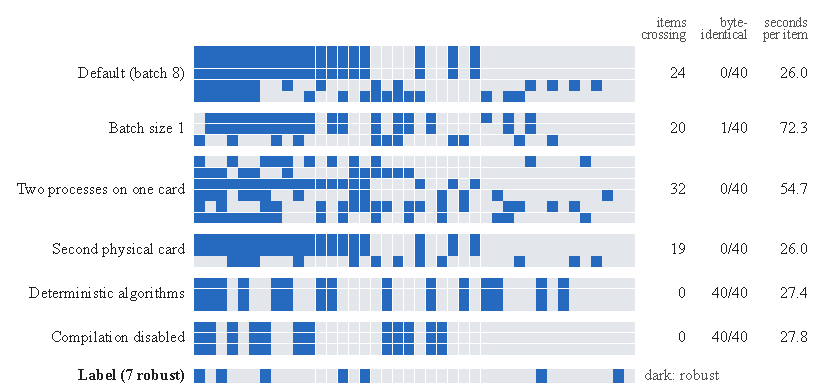
\includegraphics[width=\linewidth]{fig_rumore.pdf}
\caption{Predictions of the official pipeline for 40 preliminary public problems (columns) in 23 executions on DeepSeek (rows), by configuration; the last row is the label, dark cells are robust, and columns are sorted by how often they are predicted robust. At right: items whose prediction changes across the configuration's runs (more runs, more crossings), items whose generated text is byte-identical in all of them, and seconds per item.}
\label{fig:noise}
\end{figure}

\begin{table}[t]
\caption{Repeatability of the official pipeline on DeepSeek, 40 public problems, by configuration, in the order of Figure~\ref{fig:noise}. ``Crossings'': items whose prediction changes across the configuration's runs. ``Identical'': items whose generated text is byte-identical in all runs. Cost is runtime against the default configuration. Card 0 and card 1 are the two GPUs of the same machine. With two processes on one card, any five of its six runs give 29 to 31 crossings.}
\label{tab:reexec}
\centering
\small
\begin{tabular}{@{}lllllll@{}}
\toprule
\textbf{Configuration} & \textbf{Card} & \textbf{Runs} & \textbf{Crossings} & \textbf{Identical} & \textbf{Correct per run} & \textbf{Cost} \\
\midrule
Default (batch 8) & 0 & 5 & 24/40 & 0/40 & 24, 24, 24, 23, 24 & reference \\
Batch size 1 & 0 & 3 & 20/40 & 1/40 & 20, 21, 24 & +178\% \\
Two processes on one card & 0 & 6 & 32/40 & 0/40 & 24 to 28 & +110\% \\
Second physical card & 1 & 3 & 19/40 & 0/40 & 24, 24, 21 & +0\% \\
Deterministic algorithms & 0 & 3 & 0/40 & 40/40 & 24, 24, 24 & +5\% \\
Compilation disabled & 1 & 3 & 0/40 & 40/40 & 25, 25, 25 & +7\% \\
\bottomrule
\end{tabular}
\end{table}

\paragraph{Two candidate remedies.} Deterministic algorithms (PyTorch's, in warn-only mode, with deterministic cuDNN and a fixed cuBLAS workspace; Appendix~\ref{app:C}) and disabled compilation each made the generated text byte-identical in three sequential runs, at 5 to 7\% runtime cost. On card 0, the default configuration produced 24 crossings in five runs. Each remedy ran on one card where the default had produced crossings, each run in a new process, with no other process on that card. Three identical runs are weak evidence: the default configuration also gave three identical runs on card 0 before its fourth diverged, and five of its eight runs on the two cards shared one output. The two remedies produced different outputs, predicting 15 and 12 of the 40 problems robust, and because they ran on different cards we cannot tell whether the difference comes from the configuration or from the card. Neither gained more than one item (24 and 25 correct).

\paragraph{Distinct outputs.} The 23 executions fall into 14 distinct outputs, byte-identical within each. The same output appeared on both cards, and two runs launched in the same second on one card produced different outputs, so the output is not a property of the card alone; what selects it is not established. As only 7 of the 40 problems are robust and crossings largely cancel, accuracy moved much less than predictions: 21 to 24 correct in the default configuration on either card and 24 to 28 with two processes on one card, always below the 33 of the majority constant. An exploratory repetition of the official score extraction, whose third run ranks the 164 labeled problems at Spearman 0.24 against the first two, is in Appendix~\ref{app:C}.

\section{Regenerating the labels with our own protocol}\label{sec:labels}

\paragraph{Our labeling protocol.} We identified the organizers' perturbation families in the preliminary data (rephrase, rename, domain, distract, typos), regenerated them with gpt-oss-120b prompted with public examples, and gated each variant with gpt-oss-120b. An answer counts as correct when it matches gpt-oss-120b's answer on the original problem, because the preliminary data carry no answers; we did not check this key against the answers of the collections the problems come from. On the organizers' machine, with vLLM 0.28.0 [8] outside the official image, we labeled four models with two independent draws of variants (A and B, about 40 accepted variants per problem): 10 samples on the base problem and one per variant, at temperature 0.6, top-p 0.95 and at most 16,384 new tokens. Draw A's variants were also re-sampled with a new seed (A$'$). A label is robust when at least 6 of the 10 base samples are correct and every variant is answered correctly; unlike the earlier rule's conjunction, this requires the base problem to be solved.

A chain that reaches our cap is scored by the last boxed answer it contains, and counts as wrong without one; the organizers also count a response that reaches their limit without a parseable final answer as wrong [4]. Our protocol differs from the organizers' in perturbations, answer key, rule and sampling (one answer per variant, against 10 in the files behind most of their DeepSeek labels). Its decoding differs from the settings they publish, and its prompt may differ from the one behind their labels, which they have not stated.

\begin{table}[t]
\caption{Agreement of labels regenerated with our protocol: Cohen's kappa. The three columns for A and B treat variant chains that reached the 16,384-token cap in three ways: scored as in the protocol (by their last boxed answer, if any), dropped, or all counted as correct. The first of these columns and the A and A$'$ column give 95\% percentile bootstrap intervals over problems, and the script of Appendix~\ref{app:E} gives them for the other two. A problem has a label in a draw when it has at least one accepted variant (160 in A, 159 in B). Kappa between A and B uses the 159 problems labeled in both (150 for Qwen3.5-4B and 156 for DeepSeek when truncated chains are dropped), and between A and A$'$ 160. ``At cap'': percentage of variant chains that reached the cap in draws A and B. ``Robust'': percentage of problems labeled robust in draw A, as scored. The last column gives kappa of draw A with the organizers' preliminary DeepSeek labels: on the 138 published ones, and on the 160 that include 22 labels we derived (Section~\ref{sec:data}).}
\label{tab:label}
\centering
\small
\setlength{\tabcolsep}{3pt}
\begin{tabular}{@{}llllllll@{}}
\toprule
& & & \multicolumn{3}{l}{\textbf{A and B, truncated variant chains}} & & \\
\cmidrule(lr){4-6}
\textbf{Model} & \textbf{At cap} & \textbf{Robust} & \textbf{as scored} & \textbf{dropped} & \textbf{correct} & \textbf{A and A$'$} & \textbf{Organizers'} \\
\midrule
Skywork & 1.2, 1.5 & 74 & 0.44 [0.28, 0.59] & 0.39 & 0.39 & 0.79 [0.67, 0.89] & none \\
DeepSeek & 5.1, 6.1 & 39 & 0.41 [0.26, 0.55] & 0.35 & 0.36 & 0.46 [0.33, 0.59]$^{*}$ & 0.011; 0.025 \\
Olmo & 1.1, 0.9 & 68 & 0.38 [0.21, 0.54] & 0.39 & 0.39 & 0.65 [0.52, 0.78] & none \\
Qwen3.5-4B & 22.1, 29.2 & 9 & 0.18 [$-$0.06, 0.39] & 0.26 & 0.44 & not run & none \\
\bottomrule
\end{tabular}
\par\smallskip{\footnotesize $^{*}$On DeepSeek, A$'$ also received the answer-format line (end of this section), so this entry mixes seed and prompt.}
\end{table}

\paragraph{Results.} Under our protocol, two independent draws of variants give labels that agree at kappa 0.35 to 0.44 on Skywork, Olmo and DeepSeek, whether truncated variant chains are scored as in the protocol, dropped or all counted as correct (Table~\ref{tab:label}). On Qwen3.5-4B, 22 to 29\% of the variant chains reach the cap. Scoring these chains as in the protocol, dropping them or counting them all as correct gives agreement of 0.18, 0.26 and 0.44, and a robust share in draw A of 9\%, 83\% and 79\%. On Skywork, re-sampling the same variants with a new seed agrees far more than drawing new variants (0.79 against 0.44), so its label depends more on the variants than on the seed; on Olmo the gap is smaller (0.65 against 0.38), and on DeepSeek, where A$'$ also changed the prompt, it is 0.46 against 0.41.

Draw A's DeepSeek labels agree with the 138 labels the organizers published at kappa 0.011 [$-$0.13, 0.17], and with the 160 that include 22 of our derived labels at 0.025 [$-$0.12, 0.18]. Of the 36 problems with a published robust label, draw A calls 20 non-robust, and 4 of these change when truncated variants all count as correct. Of the 102 with a published non-robust label, draw A calls 44 robust. The reliability of the organizers' labels remains unmeasured. A retrospective calculation on the same saved answers with the main-phase threshold rule, applied as its pre-registration fixed it, with no filter on the base problem (Appendix~\ref{app:C}), gives test-retest point estimates between 0.34 and 0.56, below the pre-registered bar of 0.60, though three of the four intervals include it.

\paragraph{The prompt changes our labels.} In a first run with the bare problem text, later discarded, \mbox{Qwen3.5-4B} gave a final answer in the expected format in only 5 of its 1,640 base samples in draw A. With one instruction line requesting the format, 145 of 164 problems passed the base condition, against none. DeepSeek passed it on 147 of 164 with or without that line; its draws A and B ran without the line and A$'$ with it, and on the same variants its robust share moved from 39\% to 51\% of the 160 labeled problems, a change that mixes prompt and seed. Under our protocol, the label of Qwen3.5-4B therefore depends on the prompt. Whether this affects the organizers' labels is unknown: their baselines repository has a solve prompt that asks for an ANSWER line, but they have not said whether it was used for labeling (R3).

\section{The falsification campaign}\label{sec:campaign}

Table~\ref{tab:campaign} summarizes the campaign; Appendix~\ref{app:A} lists all 31 entries and explains three traps (rule T, the oracle H13, the duplicated pairs behind H2) and two pitfalls of the data. All entries use the preliminary data, except H16 to H18, which were scored on the 17 items of the warmup evaluation task.

\begin{table}[t]
\caption{The campaign in brief, in 19 of its 31 entries (Appendix~\ref{app:A} lists all). Ground truth is DeepSeek's and the preliminary pairs' unless stated; accuracy differences are in points against each pre-registration's baseline. H1, H7 and T count the 52 duplicated DeepSeek pairs twice; counted once, no verdict changes.}
\label{tab:campaign}
\centering
\small
\begin{tabular}{@{}L{5.5cm}L{1.9cm}L{5.6cm}@{}}
\toprule
\textbf{What we tested} & \textbf{Entries} & \textbf{Outcome} \\
\midrule
Text features; robustness as a property of the problem; labels, base accuracy and difficulty order across models & H1 to H5, H7 & rejected; H2 gained only when the duplicated pairs were counted twice \\
Official uncertainty features, logistic regression & H10 & 0.774 against a majority constant of 0.756, within the 0.692 $\pm$ 0.101 of the proposal [1] (method substituted) \\
Features cached for other models; per-target thresholds & H12, H13 & H12 rejected; the H13 ceiling withdrawn, $-$2.8 points when forced to rank \\
Our perturbation families, translation, self-consistency, the organizers' families regenerated (pilot), representation shift & H19, H22, H30 to H33 & rejected: kappa at most 0.02, AUROC at most 0.615 \\
Probes on DeepSeek's hidden states: ours and the organizers' published artifact & H36, H35 & survive their nulls; ours adds no detectable gain over length, and the artifact's score is probably in-sample \\
Trivial-robust rule, post hoc & T & a trap: +6.0 points on the preliminary pairs, +0.0 on \texttt{val-sample} \\
Identical bundles re-executed (warmup, 17 items) & H18 & noise confirmed: 11, 9, 11 and 11 correct \\
\bottomrule
\end{tabular}
\end{table}

\paragraph{Length and probes.} The character count of the problem alone orders the 164 DeepSeek labels at AUROC 0.704. Our logistic probe on DeepSeek's last-token hidden states, with layer and regularization chosen by inner cross-validation, reaches 0.710 out of fold with the original fold assignment. Over 20 other assignments, passed through the second-stage model below, it gives 0.57 to 0.76 (mean 0.69). Its scores correlate with length at Spearman +0.55, and residualized on log character count it gives 0.62. Its permutation null, rerun with 1{,}000 permutations of the whole nested procedure (the first version used 60, where 500 were pre-registered), gives $p = 0.002$. Restricted to the 138 published labels, these out-of-fold scores give 0.714 and length 0.733; retrained on those 138 alone with H36's procedure and seed, the probe gives 0.620. Combined with length in a second-stage model fitted on common outer folds, the probe changes AUROC over length alone by +0.005 on the 164 labels and by $-$0.010 on the 138 published ones (median bounds of the per-assignment 95\% intervals: $-$0.03 to 0.04, and $-$0.04 to 0.02): we detect no gain from adding the probe to length (Appendix~\ref{app:C}). This analysis replaces an earlier combination that leaked labels (Appendix~\ref{app:D}).

The organizers' published DeepSeek probe artifact orders the 164 DeepSeek labels at 0.739 with the aggregation we pre-registered and at 0.709 with its own, and at 0.62 and 0.57 residualized on log character count; its controls trained on shuffled labels give 0.68 at layer 31. The artifact does not record its training data; we infer that 137 of the 164 problems were among the public rows it was trained on, so these scores are probably largely in-sample. These length controls, which play the role of control tasks [7], were post hoc. Whether either probe reads anything beyond length that bears on robustness is not established. Apart from the three traps of Appendix~\ref{app:A}, no signal we scored by accuracy beats the majority constant by more than about one standard error on the preliminary labels, most of them DeepSeek's.

\section{Our entries}\label{sec:entries}

Our entry V8, pre-registered on 13 September, is the whole rule \texttt{return~[len(p)~>=~98 for~p~in~problems]}, with the threshold at the lower median of the 174 preliminary problems and the direction fixed on the preliminary pairs. On the original main-phase tasks it scored 11/21 and 10/19, like our entry v6 and the organizers' own entries. None of these beat the majority constant, which scores at least 11/21 and 10/19 on these tasks, and on so few items the ties do not show that length carries no signal (95\% Wilson intervals 0.32 to 0.72 and 0.32 to 0.73). On the 71 labeled rows of the official training set (revision of 17 September; 36 distinct problems), V8 differs from the all-robust constant on only 6 rows and is wrong on all 6 (46/71 against 52/71): too few to say what length is worth on official data. On the replacement tasks of 16 September, before and after the evaluation changed on 15 October [6], it predicted robust for every item (10/21 and 7/14), like an all-robust control. For the final test we nominated V8 (Codabench 1016713) and the constant (1016732), both on the Main track; our pre-registered predictions will be scored there (Appendix~\ref{app:B}).

\section{Recommendations}\label{sec:recs}

These rest mostly on DeepSeek and the preliminary data, and should be checked on the other models.
\begin{itemize}
\item \textbf{R1. Remove the variation between runs, and test the remedy:} on the same card with independent restarts, under load and across cards.
\item \textbf{R2. Repeat only where it decides something:} at the warmup's re-execution noise (a standard deviation of 1.0 item on 17, itself estimated from four runs), a one-item gap needs about eight runs per entry to reach two standard errors, so repeat only entries that run a model and sit near a prize boundary.
\item \textbf{R3. Say which prompt and decoding settings produced each released label file,} at least after the close.
\item \textbf{R4. Measure the label's reliability directly,} with two independent draws of variants labeled by the official process.
\item \textbf{R5. Show floors and noise on the leaderboard:} a row per constant predictor, the re-execution noise and binomial intervals.
\item \textbf{R6. Require a length control in white-box ablations.}
\item \textbf{R7. Remove the leaking field} \texttt{permutation\_type} from the aggregated datasets (Appendix~\ref{app:A}).
\end{itemize}

\paragraph{Code and data.} Our code, bundles, pre-registrations and outcome files are released at \href{https://github.com/Dan23RR/aimo-instrument}{\nolinkurl{github.com/Dan23RR/aimo-instrument}}. Its folder \texttt{reproduce/} recomputes the main tables from saved outputs and the six preliminary datasets, and the other numbers come from the dated records in \texttt{archive/} (Appendix~\ref{app:E}).

%%%%%% End of the main text: the six pages end here; the Limitations do not count %%%%%%
\label{fine-testo}

\section*{Limitations}

\begin{enumerate}[leftmargin=1.6em, itemsep=2pt, topsep=4pt, parsep=0pt]
\item \textbf{Preliminary data, not official data.} We did not repeat our label and probe analyses on the official training set, beyond the evaluation of V8 and a five-row check of our labels (Appendix~\ref{app:C}). Findings on label reliability and predictability may not generalize to the official evaluation setting.
\item \textbf{Our protocol, not the official one.} We did not regenerate labels with the organizers' published settings (100,000 tokens, temperature 1.0), with 10 answers per variant as in the files behind most DeepSeek labels, or on \texttt{train-main-v2}. The three treatments of truncated variant chains show how much our cap moves agreement between our draws; all three score base samples that reach the cap as the protocol does, and none of them reproduces longer decoding or a different temperature. Our low agreement with the organizers' labels is a fact about our process.
\item \textbf{One model.} We ran the probes, the re-execution study of Section~\ref{sec:reexec} and the comparisons of our regenerated labels with the organizers' preliminary labels only on DeepSeek.
\item \textbf{Re-execution.} We did not run the two candidate remedies on the same card, so card and configuration are confounded; we did not test either remedy under contention or on both cards, and we used 40 problems and one image.
\item \textbf{Records.} Some analyses rest on re-created scripts or dated records (Appendix~\ref{app:D}). Nothing here estimates performance on the final held-out problems.
\end{enumerate}

\section*{AI usage statement}

In this work, we used one generative AI tool, Claude (Anthropic), through Claude Code, for ideation, coding, analysis and writing. Ideation: it drafted the pre-registrations, including hypotheses, predictions and kill criteria, and searched and summarized the literature and the public records, including the organizers' Discord channels and the author's correspondence with them. Coding: it wrote the solution code of our bundles and the analysis and extraction scripts, ran them, and operated the organizers' virtual machine over SSH. Analysis: it computed and interpreted the results and ran automated adversarial reviews of hypotheses, drafts and code. Writing: it drafted the correspondence, this report and its revision after review.

It also made most of our Codabench uploads through the author's browser at the author's instruction. There were two exceptions: one resubmission (925822, 14 September), made without a specific instruction, and one submission that the author had not approved, sent in error and rejected before import (1016734, 28 October).

Language models were also components of our method: gpt-oss-120b generated and gated the perturbation variants and supplied the reference answers of Section~\ref{sec:labels}, and phi-4 translated problems for H22. The final decisions on the direction of the work, on the submissions (with the two exceptions above), on the nominations for the final test and on the claims of this report were the author's, and the author sent all correspondence personally. The author has reviewed all AI-assisted work and takes full responsibility for the final content of this report.

\begin{ack}
We thank Michal Štefánik, Róbert Belanec and the AIMO Interpretability team for the compute grant, a virtual machine with two GPUs, and for answering our questions; on 2 November they confirmed that the measurements taken on their machine may appear in this report. We also thank the three reviewers and the program chairs: two reviewers checked our analyses against the released code and data, and their checks corrected several of our claims. Other GPU time was rented on Modal and paid by the author or covered by Modal's platform credit. This work received no other funding, and the author has no competing interests.
\end{ack}

\section*{References}
{\small
[1] M. Štefánik, P. Mondorf, A. Waldis, Q. Liu, C. Yang, M. Spiegel, J. Kuchař, M. Kadlčík, A. Vawda-Oomerjee, C. Liu, S. Frieder, B. Plank, F. Barez and P. Stenetorp. AIMO Interpretability Challenge. CoRR, abs/2607.13899, 2026. doi:10.48550/arXiv.2607.13899.

[2] H. He and Thinking Machines Lab. Defeating Nondeterminism in LLM Inference. Thinking Machines Lab: Connectionism, 2025.

[3] J. Yuan, H. Li, X. Ding, W. Xie, Y.-J. Li, W. Zhao, K. Wan, J. Shi, X. Hu and Z. Liu. Understanding and Mitigating Numerical Sources of Nondeterminism in LLM Inference. NeurIPS 2025. arXiv:2506.09501.

[4] AIMO Interpretability Challenge website and FAQ. \url{https://aimo-interp.github.io} (accessed 28 October 2026), and its source repository aimo-interp/aimo-interp.github.io on GitHub.

[5] aimo-interp/getting-started and aimo-interp/baselines, GitHub repositories: README and issues \#6 and \#10 of getting-started; aimo-interp datasets on Hugging Face, including \texttt{train-main-v2} and \texttt{val-sample}.

[6] AIMO Interpretability Challenge Discord, \#announcements and \#qa: 5, 15 and 22 September, 9, 15, 16 and 20 October 2026.

[7] J. Hewitt and P. Liang. Designing and Interpreting Probes with Control Tasks. EMNLP-IJCNLP 2019.

[8] W. Kwon et al. Efficient Memory Management for Large Language Model Serving with PagedAttention. SOSP 2023.

[9] D. Hendrycks et al. Measuring Mathematical Problem Solving With the MATH Dataset. NeurIPS 2021 Datasets and Benchmarks Track. arXiv:2103.03874.
}

%%%%%% End of the references %%%%%%
\clearpage
\appendix
\raggedright

\section{The hypotheses, three traps and two pitfalls of the preliminary data}\label{app:A}

Section~\ref{sec:campaign} summarizes these entries. Unless stated, the ground truth is the 335 public pairs for H1 to H9 and T, the other models' preliminary labels for H12 to H15, the 17 items of the warmup evaluation set for H16 to H18, and DeepSeek's labels for the others. Validation that fits on some problems and tests on others is grouped by problem. The cross-model tests H7 and H12 to H15 hold out the model but not the problem, so part of them is in-sample; H7, H12, H14 and H15 were rejected anyway, and H13 is withdrawn. Numbers are accuracy points against each pre-registration's baseline unless they are kappa or AUROC.

{\small\setlength{\tabcolsep}{4pt}\renewcommand{\arraystretch}{1.2}
\begin{longtable}{L{1.1cm}L{3.9cm}L{5.6cm}L{2.0cm}}
\toprule
\textbf{ID} & \textbf{Hypothesis} & \textbf{Result} & \textbf{Verdict} \\
\midrule
\endfirsthead
\toprule
\textbf{ID} & \textbf{Hypothesis} & \textbf{Result} & \textbf{Verdict} \\
\midrule
\endhead
\bottomrule
\endlastfoot
H1 & The problem text predicts robustness (32 features) & 0.675 against 0.761, $-$8.7 ($-$7.4 with the duplicated pairs counted once) & rejected \\
H2 & Robustness is a property of the problem & with the 52 duplicated pairs counted once, z~=~0.88 and $-$1.3 against the per-model majority (bar 4.0); z~=~4.04 and +3.4 only when they are counted twice & rejected \\
H3 & One model's label predicts another's & $-$7.3 & rejected \\
H4 & One model's base accuracy predicts another's robustness & $-$11.8 & rejected \\
H5 & The difficulty order transfers across models & $-$25.4 & rejected \\
H6 & The same, with the oracle number of positives & $-$13.0 & ceiling (no kill criterion) \\
H7 & Base accuracy beats the prior on held-out models & $-$1.2 against the per-model majority that its pre-registration named (+0.0 against the global prior we used instead) & rejected \\
T & Robust if and only if base accuracy is below 0.05 (post hoc; see the traps below) & +6.0 on the 335 public pairs, +0.0 on \texttt{val-sample} & trap (no kill criterion) \\
H10 & The official uncertainty features reach the accuracy the proposal reports & 0.774 against a majority constant of 0.756, within 0.692 $\pm$ 0.101 [1]; a logistic regression on 13 of the 14 features of our own A100 re-implementation of the extraction (three of them constant), substituted for the official regressor & confirmed (method substituted, not declared at the time) \\
H11b & Length, saturation and trend features add signal & $-$1.8 and $-$2.5 & rejected \\
H12 & A cached model's uncertainty features predict other models & $-$16.5 & rejected \\
H13 & The same, with a threshold chosen per target & +7.3, from thresholds chosen on the scored items; $-$2.8 when forced to rank & withdrawn (no kill criterion) \\
H14, H15 & Calibration by the target's rate or by the global rate & $-$2.8 and $-$10.1 & rejected \\
H16 & Every model measured by itself beats the constant & 10/17 against 9/17 on one execution, inside the noise of H18 & survives, within noise \\
H17 & A gpt-oss threshold calibrated on \texttt{val-sample} beats H16 & 11/17, then 9, 11 and 11 on re-execution; 9/17 meets the kill criterion & not established \\
H18 & Identical bundles score differently across executions & 11, 9, 11 and 11 correct & confirmed (no kill criterion) \\
H19 & Our five mechanical perturbation families reproduce the organizers' preliminary label & accuracy 0.354 against 0.788, kappa 0.02 & rejected \\
H20 & A threshold tuned on our label transfers & 0.212 against 0.788 & rejected \\
H22 & Stability under translation reproduces the organizers' preliminary label & 0.507 against 0.740, kappa $-$0.10 & rejected \\
H23 & A threshold tuned on it transfers & +0.0 & rejected \\
H29 & Representation-distance features are repeatable (gate; written plan, not a frozen pre-registration) & ICC 0.997 to 0.999, from the dated outcome file & passes \\
H30 & The representation shift under perturbation predicts the label (written plan) & AUROC 0.615, below the kill threshold of 0.655; character count 0.704 (0.705 in E11's own computation) & rejected \\
H31 & The direction of that shift predicts the label (written plan) & AUROC 0.555 & rejected \\
H32 & The organizers' families, regenerated (pilot), reproduce their label & kappa $-$0.001 on four families, $-$0.030 with all five & rejected \\
H33 & Self-consistency over 8 samples predicts the label & AUROC 0.502 & rejected \\
H35 & The organizers' published probe artifact orders the 164 DeepSeek labels & 0.739 under the pre-registered aggregation and 0.709 under its own; 0.62 and 0.57 once residualized on log character count; its shuffled-label controls give 0.68 at layer 31 & survives its null; probably in-sample, not separated from length \\
H36 & Our linear probe, nested cross-validation, orders the 164 DeepSeek labels & 0.710 out of fold, above its permutation null, and 0.62 once residualized on log character count; 0.714 against 0.733 for length on the 138 published labels (Appendix~\ref{app:C}) & survives its null; no detectable gain over length \\
E13b-1 & Under the main-phase rule our regenerated label is test-retest reliable (kappa at least 0.60 on 3 of 4 models) & 0.34 to 0.56, retrospective (Appendix~\ref{app:C}) & rejected \\
E13b-2 & Under the main-phase rule it agrees with DeepSeek labels we computed with that rule from the preliminary data (kappa at least 0.40) & 0.02 [$-$0.09, 0.13] & rejected \\
E13b-3 & The labeling rule drives the instability of our regenerated labels & a gain of at least 0.15 on 2 of 4 models, where 3 were required; 0 of 4 on common problems & rejected \\
\end{longtable}
}

Not in the table are H8, H9, H21, H24 and H25 to H28. H8 is an oracle ceiling: 0.774, +1.8 points against the global constant and +0.4 against the per-model majority, with the duplicated pairs counted once. The outcome of H9 became rule T. H21 and H24 needed H19 and H20, and H22 and H23, to survive, so they were not run. H25 to H28 are entries of the E11 plan that its outcome file does not report under these identifiers. H25 is an anomaly of our own re-implementation of the extraction, found before the plan. H26 is the list field of the first pitfall below. H27 is a label-noise ceiling, which the plan itself closed with a resampling estimate instead of a test. H28 is the text-only baseline, which became character count (Appendix~\ref{app:D}). Three further E11 tests were not run (Appendix~\ref{app:D}). V4, an entry submitted once against its own pre-registered rule, is in Appendix~\ref{app:D}.

\paragraph{Three traps.} Rule T gains six points on the public pairs and nothing on \texttt{val-sample}, because the trivially robust items (base accuracy 0, robust under the conjunction) are absent there. The oracle H13 chose each target's threshold among all cut points on the very items it was scored on; forced to rank the items and to predict the true number of positives, it gave $-$2.8. H2 owed its survival to one measurement published under two model names and counted twice; counted once, its z falls from 4.04 to 0.88.

\paragraph{Two pitfalls of the preliminary data.} In the three aggregated datasets, the field \texttt{permutation\_type} is a list if and only if the item is robust, because the aggregation merges all perturbation types into one row for robust items and keeps one row per retained type otherwise, usually a single type. The rule ``robust if the field is a list'' reproduces all 223 labeled rows of the three datasets, and the field does not exist at inference (recommendation R7). And 20 of the 80 robust pairs among the 335 have base accuracy 0. None of them carries a published label, so they are robust only under the conjunction we used to derive their labels, while \texttt{val-sample} has no labeled pair with base accuracy below 0.05.

\section{Pre-registered predictions for the final evaluation}\label{app:B}

P1 was written on 7 September 2026, P-V8 on 13 September and P-V8b on 21 September. They are translated from the dated files and shortened. We omit the runtime predictions (under 60 seconds), which we could not score because the bundles log no runtime. A second prediction written with P1 on 7 September concerns another participant's final score and is not reported here.

\begin{itemize}
\item \textbf{P1.} The top-ranked entry's accuracy on the final held-out problems will lie within two binomial standard errors of that set's majority-class constant.
\item \textbf{P-V8.} If the organizers had neutralized length, V8 would score between 0.45 and 0.55 on both tracks (stated beforehand as the most likely outcome); if they had not, and the set was balanced, about 0.66. Observed on the original tasks: 0.52 and 0.53, inside the first band; on 21 and 19 items, however, 0.66 lies inside the 95\% intervals of both scores, so the scores do not exclude the second.
\item \textbf{P-V8b}, on the replacement tasks: the same bundles work with the new ingestion and score 6 to 15 of 21 and 4 to 10 of 14. Observed: coverage 1.0, no invalid predictions, 10/21 and 7/14, inside the bands but degenerately, since the rule predicted robust for every item.
\end{itemize}

\section{Protocols, run manifest and recalculations}\label{app:C}

\paragraph{Hardware and software.} The generation runs used the organizers' virtual machine with two NVIDIA RTX PRO 6000 Blackwell Server Edition GPUs (96 GB each), the evaluation workers' model, from 8 September 2026. Each run used one GPU; the Olmo-3-7B-Think A$'$ labels combine two runs, one on each card (below).
\begin{itemize}
\item \textbf{Official runtime image.} Section~\ref{sec:reexec} and the official score channel (E16) ran inside it: {\footnotesize\path{ghcr.io/aimo-interp/aimo-codabench-runtime:torch2.12.1-cuda13.2-cudnn9-transformers5.13.0-sklearn1.8.0-kernels0.15.2}}, digest {\footnotesize\path{sha256:fb4dab6343de7ce022ddd7906493f9ced16ff9008d497326a781d1e5adc8207a}}. They used the official extraction and regressor as shipped in our bundles: greedy decoding, at most 4,096 new tokens, static cache, batch 8.
\item \textbf{Labeling environment.} Section~\ref{sec:labels} ran with vLLM 0.28.0, torch 2.13.0 and transformers 5.16.1 (driver 610.57.04 with CUDA 13.3 on the machine, CUDA 13.0 runtime libraries in the environment) in a separate environment on the same machine; \texttt{vm\_backup/AMBIENTE\_VM\_2026-09-17.txt} lists every package.
\item \textbf{Model revisions.} Hugging Face snapshot hashes: Qwen3.5-4B \texttt{851bf6e8}, Skywork-OR1-Math-7B \texttt{fcef970f}, Olmo-3-7B-Think \texttt{d97e442d}, DeepSeek-R1-0528-Qwen3-8B \texttt{6e8885a6}, gpt-oss-120b \texttt{b5c939de}. The full hashes are in the run logs.
\item \textbf{Analyses.} They ran on CPU: E13's analysis and E15's evaluation, up to 14 September, on the virtual machine (Python 3.12, NumPy 2.3.5, scikit-learn 1.9.1), the others on the author's computer (Python 3.11.12, NumPy 2.4.4 and scikit-learn 1.8.0, as recorded for the runs of September and November). The release pins every output by SHA-256 in \texttt{MANIFEST.tsv}.
\end{itemize}

\needspace{8\baselineskip}
\paragraph{Run manifest.}
\begin{itemize}
\item \textbf{Where they ran.} The scripts in \texttt{vm/} written up to 14 September (setup, generation, extraction, E13's analysis and E15's evaluation), after which the machine stayed idle, and the clean-up script of 17 September ran on the virtual machine; the later ones ran on the author's computer.
\item \textbf{Outputs} are in \texttt{vm\_risultati/} unless the table gives another path.
\item \textbf{GPU-hours} are times from the logs (\texttt{reproduce/compute\_hours.py}). They include model loading except for the E13 labels, a difference under 1\%.
\end{itemize}

{\small\setlength{\tabcolsep}{4pt}
\begin{longtable}{L{2.4cm}L{3.2cm}L{2.2cm}>{\raggedright\arraybackslash\footnotesize}p{4.8cm}}
\toprule
\textbf{Run} & \textbf{Where it ran} & \textbf{GPU-hours} & \textbf{Outputs} \\
\midrule
\endfirsthead
\toprule
\textbf{Run} & \textbf{Where it ran} & \textbf{GPU-hours} & \textbf{Outputs} \\
\midrule
\endhead
\bottomrule
\endlastfoot
E13 variants & virtual machine & 1.15 and 1.20 & \path{e13/varianti_D1.parquet}, \path{e13/varianti_D2.parquet} \\
E13 labels & virtual machine, one queue per card & 64.4, in the logs of the 11 runs of Table~\ref{tab:label} & \path{e13/etich_*.parquet} \\
E13b, main-phase rule & author's computer & CPU only & \path{e13b_regola_nuova_2026-09-21.txt} \\
E14 re-execution & virtual machine, official image & 8.4 & \path{e14/out/*.jsonl}, \path{e14/log/} \\
E15 extraction & virtual machine & under 0.1 & \path{vm_backup/estratto/work/aimo/e15/hs_*.npz} \\
E15 probes & the virtual machine's CPU on 14 September, then the author's computer & CPU only & \path{e15_*}, \path{e15r/}, \path{vm_backup/estratto/work/aimo/e15_valuta.log} \\
E16 score channel & virtual machine, official image & 5.9 & \path{e16_*.jsonl}, \path{e16nodet/} \\
\end{longtable}
}

\paragraph{Commands.} Script paths are relative to \texttt{archive/}, the working folder of the repository. The scripts in \texttt{vm/} that ran on the virtual machine use paths under \texttt{/work/aimo}. \texttt{M} stands for the model, and in E14 \texttt{C}, \texttt{r}, \texttt{g} and \texttt{t} for the configuration, repetition, card and process tag.
\begin{itemize}
\item \textbf{E13 variants.} \texttt{vm/e13\_varianti.py -{}-draw~D1 -{}-seed~20260913 -{}-n~164 -{}-k~10}, and \texttt{-{}-draw~D2 -{}-seed~20260914}. The model gpt-oss-120b generates, solves and gates the variants (prompts below).
\item \textbf{E13 labels.} DeepSeek A and B ran an earlier version of \texttt{e13\_etichetta.py} that sent the bare problem text (now \texttt{-{}-prompt~nudo}); every other run behind Table~\ref{tab:label}, DeepSeek A$'$ included, used the explicit prompt. Draw A: \texttt{vm/e13\_etichetta.py -{}-model~M -{}-cond~A -{}-draw~D1 -{}-seed~20260921 -{}-prompt~esplicito}; B: \texttt{-{}-cond~B -{}-draw~D2 -{}-seed~20260922}; A$'$: \texttt{-{}-cond~Ap -{}-draw~D1 -{}-seed~20260923}. \texttt{vm/e13\_coda.sh} launched one queue per card (its logs are in \path{vm_backup/estratto/work/aimo/}); the card 0 queue ran an earlier version that passed no \texttt{-{}-prompt} flag, so DeepSeek A$'$ got the default of \texttt{e13\_etichetta.py}, the explicit prompt.
\item \textbf{E13b.} \texttt{vm/e13b\_regola\_nuova.py}, on the saved E13 answers; retrospective (below).
\item \textbf{E14.} \texttt{vm/e14\_all.sh 40 "C0 C1 C2 C3"} and \texttt{vm/e14\_extra.sh 1 "C5 C4"}. Each run is \texttt{e14\_run.py -{}-cond~C -{}-rep~r -{}-gpu~g -{}-tag~t -{}-n~40} inside the official image: 23 runs on DeepSeek. In the 8.4 GPU-hours the two processes of each contention pair, which shared one GPU, count once (20 runs).
\item \textbf{E15 extraction.} \texttt{vm/e15\_estrai.py -{}-model~deepseek-ai/DeepSeek-R1-0528-Qwen3-8B}, with and without the official system prompt: one forward pass per problem, last input token, all 37 hidden-state indices, at most 2,048 tokens.
\item \textbf{E15 probes.} \texttt{vm/e15\_valuta.py} ran H35, H36 and the first null (60 permutations) on 14 September, on the virtual machine's CPU; its log is \path{vm_backup/estratto/work/aimo/e15_valuta.log}. The file \path{vm_risultati/e15_valuta_2026-09-14.txt} is a later run of that day, by the file times in \path{vm_backup/MANIFEST_backup_aimo_2026-09-17.txt}, that stopped with an error at the null. H35's null is the 95th percentile, 0.602, of the AUROC of 20{,}000 random scores on the same labels, in either orientation. \texttt{vm/e15\_null\_nidificato.py} reran that null on 23 September with both grids of $C$, on the author's computer. E15-R (below) is \texttt{vm/e15r\_ricalcolo.py}, given an output folder and a number of worker processes (5 on the author's computer, 14.5 hours); its outputs are in \texttt{vm\_risultati/e15r}, and since it appends to existing files, a rerun needs a new folder. H35 needs the organizers' artifact \texttt{probe\_artifact.pkl} (hash below), which we do not redistribute.
\item \textbf{E16.} \texttt{vm/e16\_all.sh} and \texttt{vm/e16\_nodet.sh}, in the official image. Of the variables that \texttt{e16\_all.sh} sets, only the cuBLAS workspace variable reaches the extraction; \texttt{e16\_nodet.sh} sets neither.
\end{itemize}

The organizers' artifact used by H35 has SHA-256 {\footnotesize\texttt{8607478c7408922a6490adb7bda34d6a7d95403b7aa62f80dd3f2649139ccdeb}}. The listed logs total 82.8 GPU-hours. Not in the table:
\begin{itemize}
\item two complete runs of Qwen3.5-4B with the bare prompt (about 13 GPU-hours, no released log);
\item a partial run of Qwen3.5-4B A$'$ with the bare prompt (1.7 GPU-hours, included in the 82.8), discarded with them;
\item a run of Olmo-3-7B-Think A$'$ on card 1 (11.0 GPU-hours, 07:19 to 18:21 UTC on 10 September, from its queue log). Card 0 reached the same condition at 14:20, resumed from its partial file with 96 of the 164 problems done and finished the other 68, so the reported A$'$ labels come from both cards.
\end{itemize}
With these, the virtual machine ran about 107 GPU-hours, plus short smoke and feasibility tests. Our earlier runs on Modal used about 12 to 13 GPU-hours, mostly on A100 GPUs, as documented in their dated outcome files: the feature extraction behind H10, its pilot, and E9 to E12.

\paragraph{What can be recomputed.}
\begin{itemize}
\item \textbf{From saved outputs.} The scripts in \texttt{reproduce/} (Appendix~\ref{app:E}), which also read the six preliminary datasets; the other numbers come from the dated records in \texttt{archive/}.
\item \textbf{On a CPU, from the released hidden states.} Our probe (H36) and E15-R can be rerun end to end. H35 also needs the organizers' artifact.
\item \textbf{Only with the original GPUs and models.} The generation runs.
\end{itemize}

\paragraph{Re-execution configurations (Section~\ref{sec:reexec}).}
\begin{itemize}
\item \textbf{C0, default:} batch 8, on card 0, five runs.
\item \textbf{C1, batch size 1.}
\item \textbf{C2, deterministic algorithms:} \texttt{torch.use\_deterministic\_algorithms(True, warn\_only=True)}, \texttt{cudnn.deterministic = True}, \texttt{cudnn.benchmark = False} and \texttt{CUBLAS\_WORKSPACE\_CONFIG=:4096:8}.
\item \textbf{C3, contention:} two identical processes at the same time on card 0, three pairs.
\item \textbf{C4, second card:} the default on card 1.
\item \textbf{C5, compilation disabled:} \texttt{TORCH\_COMPILE\_DISABLE=1}, on card 1.
\end{itemize}
Runs within a configuration were sequential, each a new process. During these runs the other card was running another of our jobs. Two pre-registered predictions failed:
\begin{itemize}
\item batch size 1 did not make generation more repeatable: three runs gave three different outputs;
\item disabled compilation was predicted to land in one of the default outputs; it was byte-identical across its runs, but in an output of its own.
\end{itemize}
\texttt{reproduce/reexecution\_table.py} recomputes Table~\ref{tab:reexec} and the numbers of Figure~\ref{fig:noise}, and lists the 14 distinct outputs.

\paragraph{Variants and labels (Section~\ref{sec:labels}).}
\begin{itemize}
\item \textbf{Few-shot pool.} The generator saw five public examples of each family, drawn from a pool of 621 public examples (original, perturbed) over the five families. The texts are the organizers' and are not redistributed. \texttt{vm\_risultati/e13/fewshot\_pool\_ids.json} lists each example's problem identifier and SHA-256 hashes, and \texttt{reproduce/fewshot\_pool.py} rebuilds the pool from the downloaded preliminary datasets (verified on 23 November 2026: 621 of 621, byte-identical).
\item \textbf{Drawing the examples.} For draw seed $s$, problem $p$ and family $f$, the five examples are \texttt{random.Random("s|p|f").sample(pool[f] without p, 5)}.
\item \textbf{Generator.} gpt-oss-120b at low reasoning effort, temperature 1.0, top-p 1.0, at most 4,096 tokens, one request per problem and family, asking for 10 variants.
\item \textbf{Gate and reference answers.} gpt-oss-120b at medium effort, temperature 1.0, at most 8,192 tokens, solves the original and each variant. A variant is accepted if its text differs from the original, the length ratio lies between 0.7 and 4.0, and the solver's answer is unchanged. The solver's answer on the original is the reference answer.
\item \textbf{Labeling.}
  \begin{itemize}
  \item \textbf{Prompt.} Each model receives the instruction line (the second block below) followed by the problem, except DeepSeek in A and B, which received the bare text.
  \item \textbf{Sampling.} Temperature 0.6, top-p 0.95, at most 16,384 new tokens (raised from 8,192 before execution, after a test in which 2 of 3 problems saturated 8,192). There are 10 samples on the base problem and one per accepted variant.
  \item \textbf{Scoring.} A chain is scored by the last boxed answer it contains. Without one, including when it was cut at the cap, it counts as wrong.
  \end{itemize}
\end{itemize}

{\footnotesize
Generator prompt:
\begin{quote}\ttfamily
You create variants of mathematics competition problems for a robustness benchmark. Perturbation type: <family>. <family instruction> The variant must be a complete, self-contained problem with exactly the same final answer as the original. Do not solve the problem. Do not add hints or solutions. Here are 5 examples of this perturbation type: Example 1 Original: <public original> Variant: <public variant> (four more examples) Now write 10 different variants of the following problem. Make them genuinely different from each other. Output each variant between <variant> and </variant> tags, and nothing else. Original: <problem>
\end{quote}
Instruction line of the labeling prompt, also used by the solver of the gate:
\begin{quote}\ttfamily
Solve the following problem. Reason step by step, then give only the final answer inside \textbackslash{}boxed\{\}.
\end{quote}
}
The five family instructions, verbatim:
\begin{itemize}
\item rephrase: ``Rewrite the problem in different words while preserving exactly its mathematical content and its final answer.''
\item rename: ``Rename the variables, people, objects or entities in the problem while preserving its mathematical structure and its final answer.''
\item domain: ``Transfer the problem to a different real-world surface domain (a different story, setting and objects) while preserving exactly the same mathematical structure and the same final answer.''
\item distract: ``Insert irrelevant but plausible additional information (extra facts, numbers or context) that does not change the problem or its final answer.''
\item typos: ``Introduce harmless typographical or formatting noise (misspellings, spacing, punctuation, capitalisation) without changing the meaning of the problem or its final answer.''
\end{itemize}

\paragraph{The main-phase rule, retrospectively (E13b).} PREREG\_E13b was written on 21 September, before any calculation under the main-phase rule but after the E13 answers had been measured, so the calculation is retrospective.
\begin{itemize}
\item \textbf{The rule.} On the saved answers, a problem is robust if the largest drop in accuracy across families is at most 0.10 and non-robust if it is at least 0.25; problems in between get no label.
\item \textbf{No base filter.} As pre-registered, the primary calculation has no filter on the base problem, so a problem the model never solves counts as robust when no family lowers its accuracy.
\item \textbf{Test-retest, primary.} Kappa between A and B is 0.34 [0.13, 0.53] on 86 problems (Qwen3.5-4B), 0.49 [0.17, 0.76] on 132 (Skywork), 0.41 [0.09, 0.69] on 133 (Olmo) and 0.56 [0.36, 0.73] on 100 (DeepSeek). Because 58 to 95\% of the problems are labeled robust, kappa stays low even where raw agreement is high.
\item \textbf{Test-retest, secondary (S1).} On problems with at least 5 of 10 correct base samples in both draws, kappa is 0.31, 0.52, 0.40 and 0.55.
\item \textbf{Against the organizers.} Against DeepSeek labels that we computed with the same rule from the accuracy drops published in the preliminary data: 0.02 [$-$0.09, 0.13] on 133 problems.
\item \textbf{Against \texttt{train-main-v2}.} On its five labeled rows that fall on our problems and models, our labels agree with the official ones on 2 (draw A, one undefined) and 3 (draw B); five rows are too few to read.
\item \textbf{Truncated chains} are scored as in the protocol here too.
\end{itemize}

\paragraph{Subsampling (E13).} Subsampling DeepSeek's variants from 2 to 40 per problem leaves the mean kappa between A and B between 0.36 and 0.47, with no upward trend: more variants per problem do not make our labels more repeatable.

\paragraph{The official score channel (E16, exploratory).} We extracted the official regressor score on DeepSeek three times for the 174 public problems with the same code and image; this measurement was not pre-registered. The first run set the cuBLAS workspace variable and gave the same scores as the second, run without it, on all 174 problems. The second and third correlate at Spearman 0.24 over the 164 labeled problems. They give AUROC 0.487 and 0.602 in the regressor's own orientation; the paired bootstrap 95\% interval of their difference, $-$0.015 to 0.246, includes zero. The ranking of the problems was not reproduced in one of two repetitions; this does not show that the signal itself changes. As 137 of the 164 problems are in the regressor's training set, this concerns the stability of its inputs, not new problems. The 5.9 GPU-hours of the manifest also include one extraction each on Qwen3.5-4B, Skywork and Olmo, which this report does not use, and a failed start on gpt-oss-120b.

\paragraph{E15-R: the probe recalculated after review.} The procedure was fixed in \texttt{vm/e15r\_ricalcolo.py} before it ran, in a run started on 23 November 2026. It uses the same hidden states, labels and nested cross-validation as H36: layers 1 to 36, $C$ in \{0.001, 0.01, 0.1, 1\}, 5 outer and 4 inner folds.
\begin{itemize}
\item \textbf{Combination with length.}
  \begin{itemize}
  \item There are 20 fold assignments on the 164 labels and 10 on the 138 published ones.
  \item The probe's scores for the outer training problems come from a nested cross-validation inside them. Its score for each outer test problem comes from a probe selected and fitted on the outer training problems.
  \item A second-stage logistic regression on log character count, on the probe score, or on both, is fitted on the outer training problems and scored on the outer test problems.
  \item The 95\% interval of the gain of ``both'' over length is a paired bootstrap over problems (2,000 resamples) for each assignment; we report the median of its bounds.
  \end{itemize}
\item \textbf{Retraining.} The nested probe is retrained on the 138 published labels alone.
\item \textbf{Permutation null.} The null of H36 is extended from 60 to 1,000 permutations of the whole nested procedure, with the seeds of the first 60 unchanged.
\end{itemize}
We fixed the decision rule before the run: if the interval of the gain includes zero, the probe adds nothing measurable to length.

\begin{center}
\small
\begin{tabular}{@{}lllll@{}}
\toprule
\textbf{Labels} & \textbf{Length} & \textbf{Probe} & \textbf{Both} & \textbf{Gain of both over length} \\
\midrule
164 (20 assignments) & 0.696 & 0.692 & 0.701 & +0.005 [$-$0.03, 0.04] \\
138 published (10 assignments) & 0.729 & 0.644 & 0.720 & $-$0.010 [$-$0.04, 0.02] \\
\bottomrule
\end{tabular}
\end{center}
Values are means over the assignments. Length and probe here are the second-stage models, cross-validated and pooled over folds, so they differ slightly from the raw values of Section~\ref{sec:campaign} (0.704 and 0.733 for character count). On the 164 labels the gain ranges from $-$0.024 to +0.023 over the 20 assignments, and its interval excludes zero in 1 of them; the probe's second-stage model alone ranges from 0.57 to 0.76. The inner cross-validation chose hidden-state index 4 in 66 of the 100 outer folds. On the 138 published labels the gain ranges from $-$0.026 to +0.012 over the 10 assignments. With H36's procedure and random seed, the probe retrained on the 138 published labels alone gives AUROC 0.620, against 0.733 for character count; the probe's second-stage model of the table ranges from 0.59 to 0.71 over its 10 assignments.

The null with 1{,}000 permutations has mean 0.4975 and 95th percentile 0.6032; 1 permutation reaches the observed 0.710 ($p = 0.002$). Its first 60 permutations reproduce the null of 23 September (mean 0.4890, 95th percentile 0.5700) to the last digit. The run stopped after 925 permutations, when the computer restarted; \texttt{vm/e15r\_riprendi.py} computed the other 75 with the same permutations and seeds.

\section{Withdrawn claims, deviations and records}\label{app:D}

\paragraph{Claims withdrawn after review.}
\begin{itemize}
\item \textbf{A bound on latent agreement.} We had corrected the kappa of 0.025 with the organizers' DeepSeek labels for our own noise and quoted about 0.27 as an upper bound on latent agreement. That needs a measurement-error model for binary labels that we had not justified.
\item \textbf{The combination of probe and length.} Its earlier second-stage cross-validation reused probe scores computed on other folds, so some training scores depended on test labels. Its numbers (0.696 for length, 0.697 for the probe, 0.714 for both) are replaced by E15-R (Appendix~\ref{app:C}).
\item \textbf{Re-execution.} We no longer infer that the output of a run is fixed when the process starts.
\item \textbf{A simulation.} A plug-in simulation of the organizers' labeling process, which we had reported as overstating test-retest agreement by about 0.4, is no longer reported. It was a model of their process, not a measurement of it.
\end{itemize}
The other changes after review are listed in the repository README.

\paragraph{Deviations from the pre-registrations.} Each pre-registration is dated before execution, and the deviations below are also recorded as notes in those files.
\begin{itemize}
\item \textbf{Not pre-registered.} E5 is documented only in its outcome file. E11 ran from a written plan without the frozen pre-registration it called for. E16 was not pre-registered, although we had told the organizers that every experiment on their machine would be.
\item \textbf{E4.} H7 was compared with the global prior of the training models instead of the pre-registered per-model majority, against which it scores $-$1.2 points.
\item \textbf{E6.} H10 was run as a logistic regression on 13 of the 14 features in place of the pre-registered regressor and threshold, and this was not declared at the time.
\item \textbf{E11.}
  \begin{itemize}
  \item Three planned primary tests were not run.
  \item A Holm correction was planned and not applied, and H30 would fail it.
  \item The confirmation set was not held out.
  \item AUROCs were computed on raw scores, with the orientation chosen on the data.
  \item Only one of the three planned layer depths (0.80, the primary one) was extracted.
  \item The six-feature text baseline of H28 was replaced by character count alone, and the two reference analyses the plan required next to every AUROC were not computed.
  \end{itemize}
\item \textbf{E13.}
  \begin{itemize}
  \item gpt-oss-120b was pre-registered for labeling and not labeled.
  \item DeepSeek's A$'$ received the answer-format line through a queueing error.
  \item The pre-registered table that mapped outcomes to readings was not followed, because it assumed our regeneration reproduces the organizers' process.
  \item The subsampling curve varied the variants per problem, where the design varied them per family.
  \item The token cap was raised from 8,192 to 16,384 before execution.
  \end{itemize}
\item \textbf{E13b.} It was written after the E13 answers had been measured (Appendix~\ref{app:C}).
\item \textbf{E14.} Its fourth measure, the repeatability (ICC) of the 14 official features, was not computed, and two of its predictions failed (Appendix~\ref{app:C}).
\item \textbf{E15.}
  \begin{itemize}
  \item It predicted that both probes would fail their nulls; both survived.
  \item H36's nested null was pre-registered with 500 permutations and the full grid of $C$. The first run (14 September) used 60 permutations and two values of $C$. It was rerun with the full grid on 23 September, and extended to 1{,}000 permutations in a run started on 23 November.
  \item The Holm correction over the two primaries was not computed.
  \item The length controls of H35 and H36 were post hoc.
  \end{itemize}
\item \textbf{V4.} The allocation entry (909843) predicted robust on the 9 warmup items of gpt-oss-120b. It combined three numbers: the share of robust items implied by public leaderboard scores of constant entries, the count of gpt-oss-120b items read from the log of our warmup submission 907310, and that model's higher robust rate in the preliminary datasets (0.40 against 0.24). Our compliance review found that without the first two, which describe the evaluation set, it reduces to the entry it modified. Its pre-registration said it would not be sent if that review refuted it; the review did, and the author submitted it once anyway, as a measurement kept off the leaderboard. It tied the entry it modified.
\end{itemize}

\paragraph{Records.} Several analyses were first run from scripts that were not saved, and were re-created and saved later. The two length-control scripts of E15 and the rerun of its null were re-created on 23 September, each checked against the logged values before use. A few figures rest only on a dated record, not on a saved per-item output: H29's repeatability, the GPU-hours on Modal, and V8's predictions on the replacement and current tasks, which come from counts its container logged.

\paragraph{Earlier corrections.} Between our first drafts and the submitted version we corrected 54 of our own statements. They are listed, with what each changed, in \texttt{CORRECTIONS.md} in the repository, and every number in this report already includes them. The main text cites English entry points (\texttt{reproduce/}); the commands of the run manifest keep the original script names, which the dated pre-registrations cite.

\section{Data, assets, release and submissions}\label{app:E}

\paragraph{Data.}
\begin{itemize}
\item \textbf{Preliminary datasets.} The six datasets published by the organizers under \texttt{aimo-interp} on Hugging Face before the main phase: \texttt{val-sample}, \texttt{augmented-sample-math}, \texttt{augmented-sample-math-full-filtered}, \texttt{augmented-sample-math-agg-filtered}, \texttt{aimo-interp-challenge-sample-full} and \texttt{augmented-sample-math-agg}. Their cards state no license. Their problems come from the MATH dataset [9] and from the AIMO 2025 reference problems, as their \texttt{dataset\_id} field records.
\item \textbf{Official training set.} \texttt{train-main-v2} at revision 23791d9 of 17 September 2026 (82 rows, 71 labeled; the organizers extended it to 94 rows on 15 October). Its card states the license as ``other''.
\item \textbf{Downloading.} \texttt{dati.py} downloads the six preliminary datasets; we do not redistribute copies of the organizers' datasets. Our analyses used the files below. Their SHA-256 values begin as follows, and \texttt{reproduce/README.md} gives them in full.

\smallskip
{\small\begin{tabular}{@{}ll@{}}
\texttt{aimo-interp-challenge-sample-full} & \texttt{b8a57039} \\
\texttt{val-sample} & \texttt{afae22a0} \\
\texttt{augmented-sample-math-agg} & \texttt{3d168c29} \\
\texttt{augmented-sample-math-agg-filtered} & \texttt{a96bf90d} \\
\texttt{augmented-sample-math} & \texttt{991b74c0} \\
\texttt{augmented-sample-math-full-filtered} & \texttt{1b62215f} \\
\end{tabular}}
\end{itemize}

\paragraph{Models and code.} The models used, with their licenses:
\begin{itemize}
\item gpt-oss-120b (OpenAI, Apache-2.0);
\item Olmo-3-7B-Think, and Olmo-3-7B-Instruct of the warmup evaluation set (Allen Institute for AI, Apache-2.0);
\item DeepSeek-R1-0528-Qwen3-8B (DeepSeek, MIT);
\item Qwen3.5-4B (Qwen, Apache-2.0);
\item Skywork-OR1-Math-7B (Skywork; no license stated on its card);
\item phi-4 (Microsoft, MIT), for the translations of H22;
\item gemma-3-27b-it (Google, Gemma Terms of Use), loaded by our warmup entries for H16 to H18.
\end{itemize}
From the organizers we used the evaluation harness, the official uncertainty-feature extraction with its DeepSeek regressor, and the DeepSeek probe artifact with its inference code (\texttt{aimo-interp/getting-started}, which states no license); from \texttt{aimo-interp/baselines} (Apache-2.0) we used three files [5]. vLLM [8] (Apache-2.0) ran the generation, gating and labeling of Section~\ref{sec:labels}.

\paragraph{Release.} In \href{https://github.com/Dan23RR/aimo-instrument}{\nolinkurl{github.com/Dan23RR/aimo-instrument}}, the folder \texttt{archive/} keeps the layout of our working folder, with the dated records gathered in \texttt{archive/records/}. The file paths cited in this report are relative to \texttt{archive/}, except \texttt{reproduce/}, \texttt{MANIFEST.tsv} and \texttt{CORRECTIONS.md}, which sit at the top of the repository next to \texttt{paper/}, this report's sources.
\begin{itemize}
\item \textbf{Contents.} The pre-registrations, outcome files, analysis scripts, extraction outputs (including the hidden states of E15), our perturbation variants, and our submission bundles as submitted. Our code is under the MIT license, and our contribution to the data under CC BY 4.0.
\item \textbf{Organizers' files.} The getting-started files inside our bundles and our variants are released with the organizers' permission of 2 November 2026. In our variant files, the rows of the original problems keep their identifiers but not their texts. Five original problems of \texttt{val-sample} remain, as submitted, in the calibration file of the v6 bundles.
\item \textbf{Not released.} Copies of the organizers' datasets, phi-4's translations of the problems (H22), the texts of the few-shot pool (\texttt{reproduce/fewshot\_pool.py} rebuilds them), our correspondence and our internal notes. Other participants' names and passages about their entries are redacted.
\end{itemize}

{\small\setlength{\tabcolsep}{4pt}
\begin{longtable}{L{3.7cm}L{6.2cm}L{3.0cm}}
\toprule
\textbf{Script in \texttt{reproduce/}} & \textbf{What it recomputes} & \textbf{Runs on} \\
\midrule
\endfirsthead
\toprule
\textbf{Script in \texttt{reproduce/}} & \textbf{What it recomputes} & \textbf{Runs on} \\
\midrule
\endhead
\bottomrule
\endlastfoot
\texttt{labels\_table.py} & Table~\ref{tab:label} and the agreement numbers of Section~\ref{sec:labels} & saved E13 answers, seconds \\
\texttt{reexecution\_table.py} & Table~\ref{tab:reexec}, the numbers of Figure~\ref{fig:noise} and the 14 outputs of Section~\ref{sec:reexec} & saved E14 outputs, seconds \\
\texttt{probe\_vs\_length.py} & the probe and length AUROCs of Section~\ref{sec:campaign}; it prints the E15-R results and computes the permutation p-value from the saved null & saved E15 outputs, seconds \\
\texttt{v8\_threshold.py} & the two parameters of V8 (Section~\ref{sec:entries}) & public datasets, seconds \\
\texttt{compute\_hours.py} & the GPU-hours of Appendix~\ref{app:C} & logs, seconds \\
\texttt{fewshot\_pool.py} & the few-shot pool of the variant generator & public datasets, seconds \\
\end{longtable}
}

\paragraph{Italian words in file names.} The scripts and folders keep their original names, which the dated pre-registrations cite. The Italian words in the names printed in this report mean:

{\small\setlength{\tabcolsep}{6pt}
\begin{tabular}{@{}llll@{}}
\toprule
\textbf{Word} & \textbf{Meaning} & \textbf{Word} & \textbf{Meaning} \\
\midrule
\texttt{dati} & data & \texttt{nidificato} & nested \\
\texttt{risultati} & results & \texttt{nudo}, \texttt{esplicito} & bare, explicit (prompt) \\
\texttt{varianti} & variants & \texttt{regola\_nuova} & new rule \\
\texttt{etichetta}, \texttt{etich} & label & \texttt{ricalcolo} & recalculation \\
\texttt{coda} & queue & \texttt{riprendi} & resume \\
\texttt{valuta} & evaluate & \texttt{costante} & constant \\
\texttt{estrai}, \texttt{estratto} & extract, extracted & \texttt{ambiente} & environment \\
\texttt{sonde} & probes (here, bundles) & & \\
\bottomrule
\end{tabular}}

\paragraph{Codabench submissions.} These are all our submissions in both phases (user \texttt{dan23rr}), read from the Codabench API on 28 October 2026; accuracy is items correct over items.
\begin{itemize}
\item \textbf{Warmup, 29 to 31 August.} Our warmup entries are 907310, 907677, 907967, 909567, 909843, 909853, 909976, 909994, 910002 and 910013. They include a constant floor (907310), the official baseline instrumented only to log its runtime (907677), and V4, the allocation entry (909843; Appendix~\ref{app:D}). The four executions of v6 (H17, H18) gave 11, 9, 11 and 11 of 17.
\item \textbf{Original main-phase tasks.}
  \begin{itemize}
  \item 912096 and 912097 are v6, the measuring entry: 11/21 and 10/19.
  \item 924969 and 924974 are V8: 11/21 and 10/19.
  \item Their parents 924968 and 924972 also produced two rejected children (924970 and 924973) and six cancelled ones.
  \item 925822 is V8 again, uploaded by the AI assistant without a specific instruction.
  \end{itemize}
\item \textbf{Replacement tasks.} 936802 and 936806 are V8: 10/21 and 7/14.
\item \textbf{Current tasks, 28 October.}
  \begin{itemize}
  \item 1016713 and 1016730 are V8, unchanged: 10/21 and 7/14.
  \item 1016732 and 1016735 are the all-robust constant: 10/21 and 7/14.
  \item 1016733 is the parent that sent the constant's Small bundle to both tasks; its child 1016734, on the Main task, was sent in error and rejected before import.
  \end{itemize}
\item \textbf{Nominated for the final test.} 1016713 and 1016732, both on the Main track.
\end{itemize}

\needspace{6\baselineskip}
\paragraph{Bundles.} Neither nominated bundle loads a model or reads data at run time. V8's two parameters were fixed on the six preliminary datasets, its only training data, and \texttt{reproduce/v8\_threshold.py} recomputes them. The bundles are in \texttt{sonde/}. The SHA-256 of each:
\begin{itemize}
\item \texttt{solution-v8-main.zip}, a single \texttt{solution.py} with the rule of Section~\ref{sec:entries}: {\footnotesize\texttt{7b70f15c51752dcf4285e477d58c541d0ecf052d833c325c0702dbbd054ffb5f}};
\item \texttt{solution-v8-small.zip}, the same with the marker file \texttt{small.txt}: {\footnotesize\texttt{0b83b55f94dc16b9852a7c2b35d71ac5787e43d81afd6396dee00fb5e011e500}};
\item \texttt{solution-costante-main.zip}, the all-robust constant: {\footnotesize\texttt{35c47bbef717a5d4c5b6c7786bddbab9d87a02483e4f417cd34fd4ecf669c67d}};
\item \texttt{solution-costante-small.zip}, the same with \texttt{small.txt}: {\footnotesize\texttt{f798c2979b136a84c22e6d994bf0228bbfeffa044ac68f7868e13859b4c6075a}}.
\end{itemize}
To reproduce our score, upload the Main bundle to task 36237 and the Small bundle to task 36241, each with only its own task selected. On the current validation tasks the expected results are 10/21 and 7/14.


\newpage
\section*{NeurIPS Paper Checklist}




\begin{enumerate}

\item {\bf Claims}
    \item[] Question: Do the main claims made in the abstract and introduction accurately reflect the paper's contributions and scope?
    \item[] Answer: \answerYes{}
    \item[] Justification: The abstract and Section 1 state the three results and their scope: the re-execution measurement on DeepSeek, labels regenerated with our own protocol, which is not the official one, and hypotheses tested mostly on DeepSeek with the preliminary public data. The Scope paragraph of Section 1 states these limits before the results.
    \item[] Guidelines:
    \begin{itemize}
        \item The answer \answerNA{} means that the abstract and introduction do not include the claims made in the paper.
        \item The abstract and/or introduction should clearly state the claims made, including the contributions made in the paper and important assumptions and limitations. A \answerNo{} or \answerNA{} answer to this question will not be perceived well by the reviewers. 
        \item The claims made should match theoretical and experimental results, and reflect how much the results can be expected to generalize to other settings. 
        \item It is fine to include aspirational goals as motivation as long as it is clear that these goals are not attained by the paper. 
    \end{itemize}

\item {\bf Limitations}
    \item[] Question: Does the paper discuss the limitations of the work performed by the authors?
    \item[] Answer: \answerYes{}
    \item[] Justification: The Limitations section after Section 7 states what we did not do: repeat the analyses on the official data, regenerate labels with the organizers' settings, run them on other models, or test the remedies under more conditions. Sections 3 to 5 qualify each result where it is stated, and Appendix D lists the withdrawn claims and the deviations from the pre-registrations.
    \item[] Guidelines:
    \begin{itemize}
        \item The answer \answerNA{} means that the paper has no limitation while the answer \answerNo{} means that the paper has limitations, but those are not discussed in the paper. 
        \item The authors are encouraged to create a separate ``Limitations'' section in their paper.
        \item The paper should point out any strong assumptions and how robust the results are to violations of these assumptions (e.g., independence assumptions, noiseless settings, model well-specification, asymptotic approximations only holding locally). The authors should reflect on how these assumptions might be violated in practice and what the implications would be.
        \item The authors should reflect on the scope of the claims made, e.g., if the approach was only tested on a few datasets or with a few runs. In general, empirical results often depend on implicit assumptions, which should be articulated.
        \item The authors should reflect on the factors that influence the performance of the approach. For example, a facial recognition algorithm may perform poorly when image resolution is low or images are taken in low lighting. Or a speech-to-text system might not be used reliably to provide closed captions for online lectures because it fails to handle technical jargon.
        \item The authors should discuss the computational efficiency of the proposed algorithms and how they scale with dataset size.
        \item If applicable, the authors should discuss possible limitations of their approach to address problems of privacy and fairness.
        \item While the authors might fear that complete honesty about limitations might be used by reviewers as grounds for rejection, a worse outcome might be that reviewers discover limitations that aren't acknowledged in the paper. The authors should use their best judgment and recognize that individual actions in favor of transparency play an important role in developing norms that preserve the integrity of the community. Reviewers will be specifically instructed to not penalize honesty concerning limitations.
    \end{itemize}

\item {\bf Theory assumptions and proofs}
    \item[] Question: For each theoretical result, does the paper provide the full set of assumptions and a complete (and correct) proof?
    \item[] Answer: \answerNA{}
    \item[] Justification: The paper has no theoretical results.
    \item[] Guidelines:
    \begin{itemize}
        \item The answer \answerNA{} means that the paper does not include theoretical results. 
        \item All the theorems, formulas, and proofs in the paper should be numbered and cross-referenced.
        \item All assumptions should be clearly stated or referenced in the statement of any theorems.
        \item The proofs can either appear in the main paper or the supplemental material, but if they appear in the supplemental material, the authors are encouraged to provide a short proof sketch to provide intuition. 
        \item Inversely, any informal proof provided in the core of the paper should be complemented by formal proofs provided in appendix or supplemental material.
        \item Theorems and Lemmas that the proof relies upon should be properly referenced. 
    \end{itemize}

    \item {\bf Experimental result reproducibility}
    \item[] Question: Does the paper fully disclose all the information needed to reproduce the main experimental results of the paper to the extent that it affects the main claims and/or conclusions of the paper (regardless of whether the code and data are provided or not)?
    \item[] Answer: \answerYes{}
    \item[] Justification: Sections 2 to 6 and Appendix C describe the data, procedures, hardware, runtime image, model revisions, configurations, prompts and decision rules. Appendix C gives the run manifest with commands and GPU-hours, Appendix D lists the deviations from the pre-registrations, and Appendix E explains how to reproduce our score.
    \item[] Guidelines:
    \begin{itemize}
        \item The answer \answerNA{} means that the paper does not include experiments.
        \item If the paper includes experiments, a \answerNo{} answer to this question will not be perceived well by the reviewers: Making the paper reproducible is important, regardless of whether the code and data are provided or not.
        \item If the contribution is a dataset and\slash or model, the authors should describe the steps taken to make their results reproducible or verifiable. 
        \item Depending on the contribution, reproducibility can be accomplished in various ways. For example, if the contribution is a novel architecture, describing the architecture fully might suffice, or if the contribution is a specific model and empirical evaluation, it may be necessary to either make it possible for others to replicate the model with the same dataset, or provide access to the model. In general. releasing code and data is often one good way to accomplish this, but reproducibility can also be provided via detailed instructions for how to replicate the results, access to a hosted model (e.g., in the case of a large language model), releasing of a model checkpoint, or other means that are appropriate to the research performed.
        \item While NeurIPS does not require releasing code, the conference does require all submissions to provide some reasonable avenue for reproducibility, which may depend on the nature of the contribution. For example
        \begin{enumerate}
            \item If the contribution is primarily a new algorithm, the paper should make it clear how to reproduce that algorithm.
            \item If the contribution is primarily a new model architecture, the paper should describe the architecture clearly and fully.
            \item If the contribution is a new model (e.g., a large language model), then there should either be a way to access this model for reproducing the results or a way to reproduce the model (e.g., with an open-source dataset or instructions for how to construct the dataset).
            \item We recognize that reproducibility may be tricky in some cases, in which case authors are welcome to describe the particular way they provide for reproducibility. In the case of closed-source models, it may be that access to the model is limited in some way (e.g., to registered users), but it should be possible for other researchers to have some path to reproducing or verifying the results.
        \end{enumerate}
    \end{itemize}


\item {\bf Open access to data and code}
    \item[] Question: Does the paper provide open access to the data and code, with sufficient instructions to faithfully reproduce the main experimental results, as described in supplemental material?
    \item[] Answer: \answerYes{}
    \item[] Justification: Our scripts, pre-registrations, outcome files, extraction outputs, bundles and variants are public at \url{https://github.com/Dan23RR/aimo-instrument} (Section 7 and Appendix E). Its folder \texttt{reproduce/} recomputes Tables 1 and 2, the numbers of Figure 1, the probe and length AUROCs, the parameters of V8, the GPU-hours and the few-shot pool from saved outputs and the six preliminary datasets. The organizers' datasets are downloaded by \texttt{archive/dati.py} rather than redistributed.
    \item[] Guidelines:
    \begin{itemize}
        \item The answer \answerNA{} means that paper does not include experiments requiring code.
        \item Please see the NeurIPS code and data submission guidelines (\url{https://neurips.cc/public/guides/CodeSubmissionPolicy}) for more details.
        \item While we encourage the release of code and data, we understand that this might not be possible, so \answerNo{} is an acceptable answer. Papers cannot be rejected simply for not including code, unless this is central to the contribution (e.g., for a new open-source benchmark).
        \item The instructions should contain the exact command and environment needed to run to reproduce the results. See the NeurIPS code and data submission guidelines (\url{https://neurips.cc/public/guides/CodeSubmissionPolicy}) for more details.
        \item The authors should provide instructions on data access and preparation, including how to access the raw data, preprocessed data, intermediate data, and generated data, etc.
        \item The authors should provide scripts to reproduce all experimental results for the new proposed method and baselines. If only a subset of experiments are reproducible, they should state which ones are omitted from the script and why.
        \item At submission time, to preserve anonymity, the authors should release anonymized versions (if applicable).
        \item Providing as much information as possible in supplemental material (appended to the paper) is recommended, but including URLs to data and code is permitted.
    \end{itemize}


\item {\bf Experimental setting/details}
    \item[] Question: Does the paper specify all the training and test details (e.g., data splits, hyperparameters, how they were chosen, type of optimizer) necessary to understand the results?
    \item[] Answer: \answerYes{}
    \item[] Justification: Appendix A gives the data splits and the grouping by problem, and Sections 5 and 6 the thresholds and how they were chosen. Section 5 and Appendix C give the probe's nested cross-validation, Section 4 and Appendix C the decoding, sampling, seeds and token cap of the regeneration, and Section 3 and Appendix C the re-execution configurations.
    \item[] Guidelines:
    \begin{itemize}
        \item The answer \answerNA{} means that the paper does not include experiments.
        \item The experimental setting should be presented in the core of the paper to a level of detail that is necessary to appreciate the results and make sense of them.
        \item The full details can be provided either with the code, in appendix, or as supplemental material.
    \end{itemize}

\item {\bf Experiment statistical significance}
    \item[] Question: Does the paper report error bars suitably and correctly defined or other appropriate information about the statistical significance of the experiments?
    \item[] Answer: \answerYes{}
    \item[] Justification: We report 95\% percentile bootstrap intervals over problems for the agreement statistics (Section 4, Table 2 and Appendix C) and Wilson intervals for V8's scores (Section 6). Appendix C adds a paired bootstrap interval for the official score channel and an interval for the gain of the probe combined with length; Section 5 and Appendix C give the permutation nulls for the probes. The accuracy differences of Appendix A carry no intervals.
    \item[] Guidelines:
    \begin{itemize}
        \item The answer \answerNA{} means that the paper does not include experiments.
        \item The authors should answer \answerYes{} if the results are accompanied by error bars, confidence intervals, or statistical significance tests, at least for the experiments that support the main claims of the paper.
        \item The factors of variability that the error bars are capturing should be clearly stated (for example, train/test split, initialization, random drawing of some parameter, or overall run with given experimental conditions).
        \item The method for calculating the error bars should be explained (closed form formula, call to a library function, bootstrap, etc.)
        \item The assumptions made should be given (e.g., Normally distributed errors).
        \item It should be clear whether the error bar is the standard deviation or the standard error of the mean.
        \item It is OK to report 1-sigma error bars, but one should state it. The authors should preferably report a 2-sigma error bar than state that they have a 96\% CI, if the hypothesis of Normality of errors is not verified.
        \item For asymmetric distributions, the authors should be careful not to show in tables or figures symmetric error bars that would yield results that are out of range (e.g., negative error rates).
        \item If error bars are reported in tables or plots, the authors should explain in the text how they were calculated and reference the corresponding figures or tables in the text.
    \end{itemize}

\item {\bf Experiments compute resources}
    \item[] Question: For each experiment, does the paper provide sufficient information on the computer resources (type of compute workers, memory, time of execution) needed to reproduce the experiments?
    \item[] Answer: \answerYes{}
    \item[] Justification: Appendix C gives the hardware (two NVIDIA RTX PRO 6000 Blackwell Server Edition GPUs with 96 GB each, on the organizers' virtual machine), the runtime image and the GPU-hours of every main run from its logs (82.8 in the released logs, about 107 with the discarded runs and the card-1 run of Olmo-3-7B-Think A$'$), the GPU-hours on Modal and the CPU time of the probe recalculation; Figure 1 gives the seconds per item of each configuration.
    \item[] Guidelines:
    \begin{itemize}
        \item The answer \answerNA{} means that the paper does not include experiments.
        \item The paper should indicate the type of compute workers CPU or GPU, internal cluster, or cloud provider, including relevant memory and storage.
        \item The paper should provide the amount of compute required for each of the individual experimental runs as well as estimate the total compute. 
        \item The paper should disclose whether the full research project required more compute than the experiments reported in the paper (e.g., preliminary or failed experiments that didn't make it into the paper). 
    \end{itemize}
    
\item {\bf Code of ethics}
    \item[] Question: Does the research conducted in the paper conform, in every respect, with the NeurIPS Code of Ethics \url{https://neurips.cc/public/EthicsGuidelines}?
    \item[] Answer: \answerYes{}
    \item[] Justification: The work analyses public benchmark data and our own submissions; the release also includes pseudonymized snapshots of the public leaderboard. It involves no human-subjects research and makes no claim about other participants' methods, and the released files have other participants' names and passages about their entries removed (Appendix E). The organizers confirmed on 2 November that the measurements taken on their virtual machine may appear in this report.
    \item[] Guidelines:
    \begin{itemize}
        \item The answer \answerNA{} means that the authors have not reviewed the NeurIPS Code of Ethics.
        \item If the authors answer \answerNo, they should explain the special circumstances that require a deviation from the Code of Ethics.
        \item The authors should make sure to preserve anonymity (e.g., if there is a special consideration due to laws or regulations in their jurisdiction).
    \end{itemize}


\item {\bf Broader impacts}
    \item[] Question: Does the paper discuss both potential positive societal impacts and negative societal impacts of the work performed?
    \item[] Answer: \answerNo{}
    \item[] Justification: The paper does not discuss societal impacts: it measures re-execution noise in a competition's evaluation pipeline and the behavior of labels regenerated with our own protocol, and its recommendations concern evaluation practice (Section 7). The ways it documents to obtain misleading scores, a field that leaks the label in development data and re-execution noise, come with the fixes we recommend (R1, R2, R5 and R7).
    \item[] Guidelines:
    \begin{itemize}
        \item The answer \answerNA{} means that there is no societal impact of the work performed.
        \item If the authors answer \answerNA{} or \answerNo, they should explain why their work has no societal impact or why the paper does not address societal impact.
        \item Examples of negative societal impacts include potential malicious or unintended uses (e.g., disinformation, generating fake profiles, surveillance), fairness considerations (e.g., deployment of technologies that could make decisions that unfairly impact specific groups), privacy considerations, and security considerations.
        \item The conference expects that many papers will be foundational research and not tied to particular applications, let alone deployments. However, if there is a direct path to any negative applications, the authors should point it out. For example, it is legitimate to point out that an improvement in the quality of generative models could be used to generate Deepfakes for disinformation. On the other hand, it is not needed to point out that a generic algorithm for optimizing neural networks could enable people to train models that generate Deepfakes faster.
        \item The authors should consider possible harms that could arise when the technology is being used as intended and functioning correctly, harms that could arise when the technology is being used as intended but gives incorrect results, and harms following from (intentional or unintentional) misuse of the technology.
        \item If there are negative societal impacts, the authors could also discuss possible mitigation strategies (e.g., gated release of models, providing defenses in addition to attacks, mechanisms for monitoring misuse, mechanisms to monitor how a system learns from feedback over time, improving the efficiency and accessibility of ML).
    \end{itemize}
    
\item {\bf Safeguards}
    \item[] Question: Does the paper describe safeguards that have been put in place for responsible release of data or models that have a high risk for misuse (e.g., pre-trained language models, image generators, or scraped datasets)?
    \item[] Answer: \answerNA{}
    \item[] Justification: We release no models and no data with a high risk of misuse. The release (Appendix E) consists of our scripts and their outputs, our labels and per-variant answers, the hidden states of one public model on public problems, our submission bundles as submitted and, with the organizers' permission, perturbed versions of public math problems.
    \item[] Guidelines:
    \begin{itemize}
        \item The answer \answerNA{} means that the paper poses no such risks.
        \item Released models that have a high risk for misuse or dual-use should be released with necessary safeguards to allow for controlled use of the model, for example by requiring that users adhere to usage guidelines or restrictions to access the model or implementing safety filters. 
        \item Datasets that have been scraped from the Internet could pose safety risks. The authors should describe how they avoided releasing unsafe images.
        \item We recognize that providing effective safeguards is challenging, and many papers do not require this, but we encourage authors to take this into account and make a best faith effort.
    \end{itemize}

\item {\bf Licenses for existing assets}
    \item[] Question: Are the creators or original owners of assets (e.g., code, data, models), used in the paper, properly credited and are the license and terms of use explicitly mentioned and properly respected?
    \item[] Answer: \answerYes{}
    \item[] Justification: Appendix E credits the models, the datasets with the sources of their problems and the revision we used, and the code we used, with the licenses stated on their pages; where no license is stated, we say so. The organizers allowed the redistribution of their files inside our bundles and of our variants on 2 November.
    \item[] Guidelines:
    \begin{itemize}
        \item The answer \answerNA{} means that the paper does not use existing assets.
        \item The authors should cite the original paper that produced the code package or dataset.
        \item The authors should state which version of the asset is used and, if possible, include a URL.
        \item The name of the license (e.g., CC-BY 4.0) should be included for each asset.
        \item For scraped data from a particular source (e.g., website), the copyright and terms of service of that source should be provided.
        \item If assets are released, the license, copyright information, and terms of use in the package should be provided. For popular datasets, \url{paperswithcode.com/datasets} has curated licenses for some datasets. Their licensing guide can help determine the license of a dataset.
        \item For existing datasets that are re-packaged, both the original license and the license of the derived asset (if it has changed) should be provided.
        \item If this information is not available online, the authors are encouraged to reach out to the asset's creators.
    \end{itemize}

\item {\bf New assets}
    \item[] Question: Are new assets introduced in the paper well documented and is the documentation provided alongside the assets?
    \item[] Answer: \answerYes{}
    \item[] Justification: Our variants, labels, extraction outputs, analysis scripts and bundles are released at \url{https://github.com/Dan23RR/aimo-instrument} (Appendix E), with the dated pre-registrations and outcome files, a README, a manifest of SHA-256 hashes and licenses (MIT for our code, CC BY 4.0 for our contribution to the data).
    \item[] Guidelines:
    \begin{itemize}
        \item The answer \answerNA{} means that the paper does not release new assets.
        \item Researchers should communicate the details of the dataset\slash code\slash model as part of their submissions via structured templates. This includes details about training, license, limitations, etc. 
        \item The paper should discuss whether and how consent was obtained from people whose asset is used.
        \item At submission time, remember to anonymize your assets (if applicable). You can either create an anonymized URL or include an anonymized zip file.
    \end{itemize}

\item {\bf Crowdsourcing and research with human subjects}
    \item[] Question: For crowdsourcing experiments and research with human subjects, does the paper include the full text of instructions given to participants and screenshots, if applicable, as well as details about compensation (if any)? 
    \item[] Answer: \answerNA{}
    \item[] Justification: The paper involves no crowdsourcing and no research with human subjects.
    \item[] Guidelines:
    \begin{itemize}
        \item The answer \answerNA{} means that the paper does not involve crowdsourcing nor research with human subjects.
        \item Including this information in the supplemental material is fine, but if the main contribution of the paper involves human subjects, then as much detail as possible should be included in the main paper. 
        \item According to the NeurIPS Code of Ethics, workers involved in data collection, curation, or other labor should be paid at least the minimum wage in the country of the data collector. 
    \end{itemize}

\item {\bf Institutional review board (IRB) approvals or equivalent for research with human subjects}
    \item[] Question: Does the paper describe potential risks incurred by study participants, whether such risks were disclosed to the subjects, and whether Institutional Review Board (IRB) approvals (or an equivalent approval/review based on the requirements of your country or institution) were obtained?
    \item[] Answer: \answerNA{}
    \item[] Justification: The paper involves no human subjects.
    \item[] Guidelines:
    \begin{itemize}
        \item The answer \answerNA{} means that the paper does not involve crowdsourcing nor research with human subjects.
        \item Depending on the country in which research is conducted, IRB approval (or equivalent) may be required for any human subjects research. If you obtained IRB approval, you should clearly state this in the paper. 
        \item We recognize that the procedures for this may vary significantly between institutions and locations, and we expect authors to adhere to the NeurIPS Code of Ethics and the guidelines for their institution. 
        \item For initial submissions, do not include any information that would break anonymity (if applicable), such as the institution conducting the review.
    \end{itemize}

\item {\bf Declaration of LLM usage}
    \item[] Question: Does the paper describe the usage of LLMs if it is an important, original, or non-standard component of the core methods in this research? Note that if the LLM is used only for writing, editing, or formatting purposes and does \emph{not} impact the core methodology, scientific rigor, or originality of the research, declaration is not required.
    %this research? 
    \item[] Answer: \answerYes{}
    \item[] Justification: Language models are the objects of study (Section 2). In our label regeneration gpt-oss-120b generated and gated the perturbation variants and supplied the reference answers (Section 4, Appendix C), and phi-4 translated problems for H22 (Appendix A). An AI assistant (Claude, through Claude Code) drafted the pre-registrations, wrote and ran the code, operated the virtual machine, made most of our uploads and drafted this report and its revision, as disclosed in the AI usage statement.
    \item[] Guidelines:
    \begin{itemize}
        \item The answer \answerNA{} means that the core method development in this research does not involve LLMs as any important, original, or non-standard components.
        \item Please refer to our LLM policy in the NeurIPS handbook for what should or should not be described.
    \end{itemize}

\end{enumerate}

\end{document}
".
\usepackage[final,sglblindworkshop]{neurips_2026}
\workshoptitle{AIMO Interpretability Challenge}
\ifdefined\cleancopy\else
  \usepackage{lineno}
  \linenumbers
  \ifdefined\everyline\else\modulolinenumbers[5]\fi
  \renewcommand\linenumberfont{\normalfont\tiny\sffamily\color{black!45}}
\fi

\usepackage[utf8]{inputenc}
\usepackage[T1]{fontenc}
%% Typewriter text in Latin Modern, the Type 1 version of the default Computer Modern typewriter, with the same
%% widths: without it, \texttt in T1 encoding becomes bitmap (Type 3) fonts, and the template asks for Type 1 fonts.
\renewcommand{\ttdefault}{lmtt}
\usepackage{hyperref}
\hypersetup{pdftitle={The Instrument Behind the Leaderboard: Re-Execution Noise and Label Regeneration in the AIMO Interpretability Challenge}, pdfauthor={Daniel Culotta}}
\usepackage{url}
\def\UrlBreaks{\do\/\do\.\do\_\do\-\do\:}
\usepackage{booktabs}
\usepackage{array}
\usepackage{longtable}
\newcolumntype{L}[1]{>{\raggedright\arraybackslash}p{#1}}
\usepackage{amsfonts}
\usepackage{microtype}
\usepackage{xcolor}
\usepackage{graphicx}
\usepackage{enumitem}
\usepackage{needspace}
\setlist[itemize]{leftmargin=1.4em, itemsep=2pt, topsep=4pt, parsep=0pt}
\setlist[itemize,2]{label=$\circ$}
\renewcommand{\arraystretch}{1.15}
\raggedbottom

\title{The Instrument Behind the Leaderboard: Re-Execution Noise and Label Regeneration in the AIMO Interpretability Challenge}

\author{%
  Daniel Culotta \\
  Independent researcher
}

\begin{document}

\maketitle

\begin{abstract}
We treat the AIMO Interpretability benchmark, which asks whether a model's answer to a math problem survives perturbations, as a measurement instrument. Almost all our label and probe analyses use the preliminary datasets. As the program chairs note, these differ from the official training and validation data in sampling, perturbations and eligibility, so findings on label reliability and predictability may not hold in the official evaluation. First, on DeepSeek-R1-0528-Qwen3-8B in the official pipeline, 24 of 40 items changed prediction across five default runs. Turning compilation off, or deterministic algorithms on, gave three byte-identical runs, each on one card. Second, we regenerated labels with our own protocol, not the official one: our perturbations and answer key, one answer per variant, a 16,384-token cap and temperature 0.6, where the organizers publish 100,000 tokens and 1.0. Two independent draws agree at kappa 0.35 to 0.44 on three of four models however truncated chains are treated, and 0.18 to 0.44 on Qwen3.5-4B, whose chains often reach the cap. Draw A agrees with the 138 published DeepSeek labels at kappa 0.01. This describes our protocol and does not measure the reliability of the organizers' labels. Third, of the 27 dated hypotheses with a kill criterion, 21 failed it. Our probe on DeepSeek's hidden states does no better than problem length (AUROC 0.710 against 0.704; below length on the published labels) and adds nothing detectable to it.
\end{abstract}

\section{Introduction}\label{sec:1}

A leaderboard is a measurement. Its score is read off an instrument made of a label, an evaluation set, an inference pipeline and the hardware it runs on. When the label is itself produced by a stochastic process, the instrument has noise of its own, which a single submission cannot see. We measure the re-execution noise of the official extraction and regressor, and the repeatability of labels regenerated with our own protocol, not the noise of the organizers' labels.

We study the instrument of the AIMO Interpretability Challenge, in which a submission predicts, for a given model and math problem, whether the model's answer is robust to perturbations of the problem [1]. We ran our work as a falsification campaign: every hypothesis was recorded in a dated file, 26 of the 31 before their data were seen, and every tested hypothesis is reported. Of the 31 entries, 27 carried a kill criterion written before their test ran (for 3 of them in a written plan rather than a frozen pre-registration, and for H2 after its concordance had been seen). By that criterion 21 were rejected, 5 survived and 1 is not established (Appendix~\ref{app:A}).

\paragraph{Scope.} Three limits apply.
\begin{itemize}
\item \textbf{Preliminary and official data.} Almost all of our label and probe analyses use the six preliminary public datasets released before the main phase. Their labels follow an earlier rule than those of the official training set (\texttt{train-main-v2}) and of the validation and test tasks [5]; as the program chairs noted in their meta-review, their sampling procedures, perturbations and eligibility criteria also differ. Beyond the label rule, we did not compare the two. Unless we say otherwise, a result on labels or on their predictability holds for the preliminary data and may not hold in the official evaluation setting.
\item \textbf{Our labeling protocol is not the official one.} When we regenerate labels (Section~\ref{sec:labels}), we use our own perturbations, prompts, sampling, decoding, answer key and labeling rule. Disagreement with the organizers' preliminary labels therefore shows that the two processes give different labels; it does not establish that their labels are unreliable or irreproducible.
\item \textbf{Mostly one model.} The re-execution study of Section~\ref{sec:reexec}, the probe analyses and every comparison of our regenerated labels with the organizers' preliminary labels are on DeepSeek-R1-0528-Qwen3-8B. Regenerated labels cover four models, but no conclusion about the official benchmark is established across models.
\end{itemize}

Within these limits, Sections~\ref{sec:reexec} to~\ref{sec:campaign} report re-execution noise and two candidate remedies, our regenerated labels, and signals that do no better than problem length or come from an artifact of the data. Nondeterminism of LLM inference is documented in general [2, 3]; we add its size for one model, one submission and 40 problems on this benchmark's hardware and pipeline. We make no claim about any participant's method.

\section{The task, the labels and the data}\label{sec:data}

\paragraph{Task.} A submission receives a model identifier, a reasoning effort and a list of problems, and returns one robustness verdict per problem, offline on one GPU within one hour [4, 5], or 70 minutes since 15 October [6]. The models are Qwen3.5-4B, Skywork-OR1-Math-7B, Olmo-3-7B-Think and \mbox{DeepSeek-R1-0528-Qwen3-8B} in both tracks, and gpt-oss-120b in the Main track only.

\paragraph{Official data.} The main-phase training set \texttt{train-main-v2} labels all five models with a threshold on the largest accuracy drop across perturbation families: robust at most 0.10, non-robust at least 0.25, no label in between [5]. The organizers' published decoding settings are up to 100,000 tokens at temperature 1.0, top-k 40 and top-p 0.95, and a response that reaches the limit without a final answer counts as wrong [4]. Since 16 September the private validation tasks have 21 items (Main) and 14 (Small), on which the binomial standard error of an accuracy near one half is 10.9 and 13.4 points; the final test uses 30 to 50 new problems [5, 6].

\paragraph{Preliminary data.} Six datasets released before the main phase aggregate to 335 (model, problem) pairs over 174 distinct problems, up to eight per problem; 52 pairs repeat the DeepSeek measurements under a second model name. Their labels follow an earlier rule: on all 379 labeled rows (a pair can have several), the label equals the conjunction ``no perturbation lowered accuracy''. A per-family majority rule (``more than half of the answers are correct in every perturbation family'') reproduces the same 379 labels, so these rows cannot tell the two rules apart. Whether they used the decoding settings above is not documented; in the files behind most DeepSeek labels, most variants listed as lowering accuracy were answered 10 times. We call their labels the organizers' preliminary labels, and keep ``official'' for \texttt{train-main-v2} and the validation and test tasks.

\paragraph{DeepSeek labels.} DeepSeek is the only evaluated model with many preliminary labels: 164 distinct problems (the 52 duplicated pairs count once). For 138 of them the data publish a label. For the other 26 we derived one with the conjunction, which makes 4 of them robust; the majority rule would make 21 robust, so these 26 labels depend on the choice of rule. We therefore report results on the 138 published labels separately.

\section{Re-execution noise on the evaluation workers' type of GPU}\label{sec:reexec}

On a virtual machine lent by the organizers, with two NVIDIA RTX PRO 6000 Blackwell Server Edition GPUs (the type the evaluation workers use), we ran 40 preliminary public problems through the official runtime image, extraction and regressor, unmodified, on DeepSeek. Decoding was greedy, with at most 4,096 new tokens in batches of 8. The 40 labels are DeepSeek's of Section~\ref{sec:data}: 28 published and 12 that we derived with the conjunction, which include 3 of the 7 robust ones. Figure~\ref{fig:noise} shows the 23 executions; Table~\ref{tab:reexec} gives the repeatability of each configuration.

\begin{figure}[t]
\centering
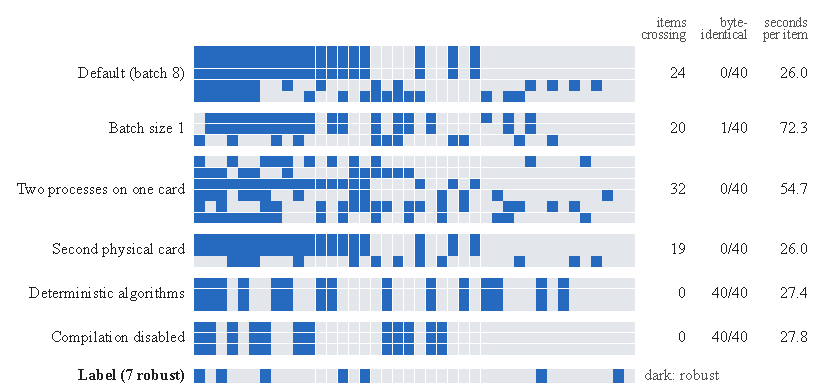
\includegraphics[width=\linewidth]{fig_rumore.pdf}
\caption{Predictions of the official pipeline for 40 preliminary public problems (columns) in 23 executions on DeepSeek (rows), by configuration; the last row is the label, dark cells are robust, and columns are sorted by how often they are predicted robust. At right: items whose prediction changes across the configuration's runs (more runs, more crossings), items whose generated text is byte-identical in all of them, and seconds per item.}
\label{fig:noise}
\end{figure}

\begin{table}[t]
\caption{Repeatability of the official pipeline on DeepSeek, 40 public problems, by configuration, in the order of Figure~\ref{fig:noise}. ``Crossings'': items whose prediction changes across the configuration's runs. ``Identical'': items whose generated text is byte-identical in all runs. Cost is runtime against the default configuration. Card 0 and card 1 are the two GPUs of the same machine. With two processes on one card, any five of its six runs give 29 to 31 crossings.}
\label{tab:reexec}
\centering
\small
\begin{tabular}{@{}lllllll@{}}
\toprule
\textbf{Configuration} & \textbf{Card} & \textbf{Runs} & \textbf{Crossings} & \textbf{Identical} & \textbf{Correct per run} & \textbf{Cost} \\
\midrule
Default (batch 8) & 0 & 5 & 24/40 & 0/40 & 24, 24, 24, 23, 24 & reference \\
Batch size 1 & 0 & 3 & 20/40 & 1/40 & 20, 21, 24 & +178\% \\
Two processes on one card & 0 & 6 & 32/40 & 0/40 & 24 to 28 & +110\% \\
Second physical card & 1 & 3 & 19/40 & 0/40 & 24, 24, 21 & +0\% \\
Deterministic algorithms & 0 & 3 & 0/40 & 40/40 & 24, 24, 24 & +5\% \\
Compilation disabled & 1 & 3 & 0/40 & 40/40 & 25, 25, 25 & +7\% \\
\bottomrule
\end{tabular}
\end{table}

\paragraph{Two candidate remedies.} Deterministic algorithms (PyTorch's, in warn-only mode, with deterministic cuDNN and a fixed cuBLAS workspace; Appendix~\ref{app:C}) and disabled compilation each made the generated text byte-identical in three sequential runs, at 5 to 7\% runtime cost. On card 0, the default configuration produced 24 crossings in five runs. Each remedy ran on one card where the default had produced crossings, each run in a new process, with no other process on that card. Three identical runs are weak evidence: the default configuration also gave three identical runs on card 0 before its fourth diverged, and five of its eight runs on the two cards shared one output. The two remedies produced different outputs, predicting 15 and 12 of the 40 problems robust, and because they ran on different cards we cannot tell whether the difference comes from the configuration or from the card. Neither gained more than one item (24 and 25 correct).

\paragraph{Distinct outputs.} The 23 executions fall into 14 distinct outputs, byte-identical within each. The same output appeared on both cards, and two runs launched in the same second on one card produced different outputs, so the output is not a property of the card alone; what selects it is not established. As only 7 of the 40 problems are robust and crossings largely cancel, accuracy moved much less than predictions: 21 to 24 correct in the default configuration on either card and 24 to 28 with two processes on one card, always below the 33 of the majority constant. An exploratory repetition of the official score extraction, whose third run ranks the 164 labeled problems at Spearman 0.24 against the first two, is in Appendix~\ref{app:C}.

\section{Regenerating the labels with our own protocol}\label{sec:labels}

\paragraph{Our labeling protocol.} We identified the organizers' perturbation families in the preliminary data (rephrase, rename, domain, distract, typos), regenerated them with gpt-oss-120b prompted with public examples, and gated each variant with gpt-oss-120b. An answer counts as correct when it matches gpt-oss-120b's answer on the original problem, because the preliminary data carry no answers; we did not check this key against the answers of the collections the problems come from. On the organizers' machine, with vLLM 0.28.0 [8] outside the official image, we labeled four models with two independent draws of variants (A and B, about 40 accepted variants per problem): 10 samples on the base problem and one per variant, at temperature 0.6, top-p 0.95 and at most 16,384 new tokens. Draw A's variants were also re-sampled with a new seed (A$'$). A label is robust when at least 6 of the 10 base samples are correct and every variant is answered correctly; unlike the earlier rule's conjunction, this requires the base problem to be solved.

A chain that reaches our cap is scored by the last boxed answer it contains, and counts as wrong without one; the organizers also count a response that reaches their limit without a parseable final answer as wrong [4]. Our protocol differs from the organizers' in perturbations, answer key, rule and sampling (one answer per variant, against 10 in the files behind most of their DeepSeek labels). Its decoding differs from the settings they publish, and its prompt may differ from the one behind their labels, which they have not stated.

\begin{table}[t]
\caption{Agreement of labels regenerated with our protocol: Cohen's kappa. The three columns for A and B treat variant chains that reached the 16,384-token cap in three ways: scored as in the protocol (by their last boxed answer, if any), dropped, or all counted as correct. The first of these columns and the A and A$'$ column give 95\% percentile bootstrap intervals over problems, and the script of Appendix~\ref{app:E} gives them for the other two. A problem has a label in a draw when it has at least one accepted variant (160 in A, 159 in B). Kappa between A and B uses the 159 problems labeled in both (150 for Qwen3.5-4B and 156 for DeepSeek when truncated chains are dropped), and between A and A$'$ 160. ``At cap'': percentage of variant chains that reached the cap in draws A and B. ``Robust'': percentage of problems labeled robust in draw A, as scored. The last column gives kappa of draw A with the organizers' preliminary DeepSeek labels: on the 138 published ones, and on the 160 that include 22 labels we derived (Section~\ref{sec:data}).}
\label{tab:label}
\centering
\small
\setlength{\tabcolsep}{3pt}
\begin{tabular}{@{}llllllll@{}}
\toprule
& & & \multicolumn{3}{l}{\textbf{A and B, truncated variant chains}} & & \\
\cmidrule(lr){4-6}
\textbf{Model} & \textbf{At cap} & \textbf{Robust} & \textbf{as scored} & \textbf{dropped} & \textbf{correct} & \textbf{A and A$'$} & \textbf{Organizers'} \\
\midrule
Skywork & 1.2, 1.5 & 74 & 0.44 [0.28, 0.59] & 0.39 & 0.39 & 0.79 [0.67, 0.89] & none \\
DeepSeek & 5.1, 6.1 & 39 & 0.41 [0.26, 0.55] & 0.35 & 0.36 & 0.46 [0.33, 0.59]$^{*}$ & 0.011; 0.025 \\
Olmo & 1.1, 0.9 & 68 & 0.38 [0.21, 0.54] & 0.39 & 0.39 & 0.65 [0.52, 0.78] & none \\
Qwen3.5-4B & 22.1, 29.2 & 9 & 0.18 [$-$0.06, 0.39] & 0.26 & 0.44 & not run & none \\
\bottomrule
\end{tabular}
\par\smallskip{\footnotesize $^{*}$On DeepSeek, A$'$ also received the answer-format line (end of this section), so this entry mixes seed and prompt.}
\end{table}

\paragraph{Results.} Under our protocol, two independent draws of variants give labels that agree at kappa 0.35 to 0.44 on Skywork, Olmo and DeepSeek, whether truncated variant chains are scored as in the protocol, dropped or all counted as correct (Table~\ref{tab:label}). On Qwen3.5-4B, 22 to 29\% of the variant chains reach the cap. Scoring these chains as in the protocol, dropping them or counting them all as correct gives agreement of 0.18, 0.26 and 0.44, and a robust share in draw A of 9\%, 83\% and 79\%. On Skywork, re-sampling the same variants with a new seed agrees far more than drawing new variants (0.79 against 0.44), so its label depends more on the variants than on the seed; on Olmo the gap is smaller (0.65 against 0.38), and on DeepSeek, where A$'$ also changed the prompt, it is 0.46 against 0.41.

Draw A's DeepSeek labels agree with the 138 labels the organizers published at kappa 0.011 [$-$0.13, 0.17], and with the 160 that include 22 of our derived labels at 0.025 [$-$0.12, 0.18]. Of the 36 problems with a published robust label, draw A calls 20 non-robust, and 4 of these change when truncated variants all count as correct. Of the 102 with a published non-robust label, draw A calls 44 robust. The reliability of the organizers' labels remains unmeasured. A retrospective calculation on the same saved answers with the main-phase threshold rule, applied as its pre-registration fixed it, with no filter on the base problem (Appendix~\ref{app:C}), gives test-retest point estimates between 0.34 and 0.56, below the pre-registered bar of 0.60, though three of the four intervals include it.

\paragraph{The prompt changes our labels.} In a first run with the bare problem text, later discarded, \mbox{Qwen3.5-4B} gave a final answer in the expected format in only 5 of its 1,640 base samples in draw A. With one instruction line requesting the format, 145 of 164 problems passed the base condition, against none. DeepSeek passed it on 147 of 164 with or without that line; its draws A and B ran without the line and A$'$ with it, and on the same variants its robust share moved from 39\% to 51\% of the 160 labeled problems, a change that mixes prompt and seed. Under our protocol, the label of Qwen3.5-4B therefore depends on the prompt. Whether this affects the organizers' labels is unknown: their baselines repository has a solve prompt that asks for an ANSWER line, but they have not said whether it was used for labeling (R3).

\section{The falsification campaign}\label{sec:campaign}

Table~\ref{tab:campaign} summarizes the campaign; Appendix~\ref{app:A} lists all 31 entries and explains three traps (rule T, the oracle H13, the duplicated pairs behind H2) and two pitfalls of the data. All entries use the preliminary data, except H16 to H18, which were scored on the 17 items of the warmup evaluation task.

\begin{table}[t]
\caption{The campaign in brief, in 19 of its 31 entries (Appendix~\ref{app:A} lists all). Ground truth is DeepSeek's and the preliminary pairs' unless stated; accuracy differences are in points against each pre-registration's baseline. H1, H7 and T count the 52 duplicated DeepSeek pairs twice; counted once, no verdict changes.}
\label{tab:campaign}
\centering
\small
\begin{tabular}{@{}L{5.5cm}L{1.9cm}L{5.6cm}@{}}
\toprule
\textbf{What we tested} & \textbf{Entries} & \textbf{Outcome} \\
\midrule
Text features; robustness as a property of the problem; labels, base accuracy and difficulty order across models & H1 to H5, H7 & rejected; H2 gained only when the duplicated pairs were counted twice \\
Official uncertainty features, logistic regression & H10 & 0.774 against a majority constant of 0.756, within the 0.692 $\pm$ 0.101 of the proposal [1] (method substituted) \\
Features cached for other models; per-target thresholds & H12, H13 & H12 rejected; the H13 ceiling withdrawn, $-$2.8 points when forced to rank \\
Our perturbation families, translation, self-consistency, the organizers' families regenerated (pilot), representation shift & H19, H22, H30 to H33 & rejected: kappa at most 0.02, AUROC at most 0.615 \\
Probes on DeepSeek's hidden states: ours and the organizers' published artifact & H36, H35 & survive their nulls; ours adds no detectable gain over length, and the artifact's score is probably in-sample \\
Trivial-robust rule, post hoc & T & a trap: +6.0 points on the preliminary pairs, +0.0 on \texttt{val-sample} \\
Identical bundles re-executed (warmup, 17 items) & H18 & noise confirmed: 11, 9, 11 and 11 correct \\
\bottomrule
\end{tabular}
\end{table}

\paragraph{Length and probes.} The character count of the problem alone orders the 164 DeepSeek labels at AUROC 0.704. Our logistic probe on DeepSeek's last-token hidden states, with layer and regularization chosen by inner cross-validation, reaches 0.710 out of fold with the original fold assignment. Over 20 other assignments, passed through the second-stage model below, it gives 0.57 to 0.76 (mean 0.69). Its scores correlate with length at Spearman +0.55, and residualized on log character count it gives 0.62. Its permutation null, rerun with 1{,}000 permutations of the whole nested procedure (the first version used 60, where 500 were pre-registered), gives $p = 0.002$. Restricted to the 138 published labels, these out-of-fold scores give 0.714 and length 0.733; retrained on those 138 alone with H36's procedure and seed, the probe gives 0.620. Combined with length in a second-stage model fitted on common outer folds, the probe changes AUROC over length alone by +0.005 on the 164 labels and by $-$0.010 on the 138 published ones (median bounds of the per-assignment 95\% intervals: $-$0.03 to 0.04, and $-$0.04 to 0.02): we detect no gain from adding the probe to length (Appendix~\ref{app:C}). This analysis replaces an earlier combination that leaked labels (Appendix~\ref{app:D}).

The organizers' published DeepSeek probe artifact orders the 164 DeepSeek labels at 0.739 with the aggregation we pre-registered and at 0.709 with its own, and at 0.62 and 0.57 residualized on log character count; its controls trained on shuffled labels give 0.68 at layer 31. The artifact does not record its training data; we infer that 137 of the 164 problems were among the public rows it was trained on, so these scores are probably largely in-sample. These length controls, which play the role of control tasks [7], were post hoc. Whether either probe reads anything beyond length that bears on robustness is not established. Apart from the three traps of Appendix~\ref{app:A}, no signal we scored by accuracy beats the majority constant by more than about one standard error on the preliminary labels, most of them DeepSeek's.

\section{Our entries}\label{sec:entries}

Our entry V8, pre-registered on 13 September, is the whole rule \texttt{return~[len(p)~>=~98 for~p~in~problems]}, with the threshold at the lower median of the 174 preliminary problems and the direction fixed on the preliminary pairs. On the original main-phase tasks it scored 11/21 and 10/19, like our entry v6 and the organizers' own entries. None of these beat the majority constant, which scores at least 11/21 and 10/19 on these tasks, and on so few items the ties do not show that length carries no signal (95\% Wilson intervals 0.32 to 0.72 and 0.32 to 0.73). On the 71 labeled rows of the official training set (revision of 17 September; 36 distinct problems), V8 differs from the all-robust constant on only 6 rows and is wrong on all 6 (46/71 against 52/71): too few to say what length is worth on official data. On the replacement tasks of 16 September, before and after the evaluation changed on 15 October [6], it predicted robust for every item (10/21 and 7/14), like an all-robust control. For the final test we nominated V8 (Codabench 1016713) and the constant (1016732), both on the Main track; our pre-registered predictions will be scored there (Appendix~\ref{app:B}).

\section{Recommendations}\label{sec:recs}

These rest mostly on DeepSeek and the preliminary data, and should be checked on the other models.
\begin{itemize}
\item \textbf{R1. Remove the variation between runs, and test the remedy:} on the same card with independent restarts, under load and across cards.
\item \textbf{R2. Repeat only where it decides something:} at the warmup's re-execution noise (a standard deviation of 1.0 item on 17, itself estimated from four runs), a one-item gap needs about eight runs per entry to reach two standard errors, so repeat only entries that run a model and sit near a prize boundary.
\item \textbf{R3. Say which prompt and decoding settings produced each released label file,} at least after the close.
\item \textbf{R4. Measure the label's reliability directly,} with two independent draws of variants labeled by the official process.
\item \textbf{R5. Show floors and noise on the leaderboard:} a row per constant predictor, the re-execution noise and binomial intervals.
\item \textbf{R6. Require a length control in white-box ablations.}
\item \textbf{R7. Remove the leaking field} \texttt{permutation\_type} from the aggregated datasets (Appendix~\ref{app:A}).
\end{itemize}

\paragraph{Code and data.} Our code, bundles, pre-registrations and outcome files are released at \href{https://github.com/Dan23RR/aimo-instrument}{\nolinkurl{github.com/Dan23RR/aimo-instrument}}. Its folder \texttt{reproduce/} recomputes the main tables from saved outputs and the six preliminary datasets, and the other numbers come from the dated records in \texttt{archive/} (Appendix~\ref{app:E}).

%%%%%% End of the main text: the six pages end here; the Limitations do not count %%%%%%
\label{fine-testo}

\section*{Limitations}

\begin{enumerate}[leftmargin=1.6em, itemsep=2pt, topsep=4pt, parsep=0pt]
\item \textbf{Preliminary data, not official data.} We did not repeat our label and probe analyses on the official training set, beyond the evaluation of V8 and a five-row check of our labels (Appendix~\ref{app:C}). Findings on label reliability and predictability may not generalize to the official evaluation setting.
\item \textbf{Our protocol, not the official one.} We did not regenerate labels with the organizers' published settings (100,000 tokens, temperature 1.0), with 10 answers per variant as in the files behind most DeepSeek labels, or on \texttt{train-main-v2}. The three treatments of truncated variant chains show how much our cap moves agreement between our draws; all three score base samples that reach the cap as the protocol does, and none of them reproduces longer decoding or a different temperature. Our low agreement with the organizers' labels is a fact about our process.
\item \textbf{One model.} We ran the probes, the re-execution study of Section~\ref{sec:reexec} and the comparisons of our regenerated labels with the organizers' preliminary labels only on DeepSeek.
\item \textbf{Re-execution.} We did not run the two candidate remedies on the same card, so card and configuration are confounded; we did not test either remedy under contention or on both cards, and we used 40 problems and one image.
\item \textbf{Records.} Some analyses rest on re-created scripts or dated records (Appendix~\ref{app:D}). Nothing here estimates performance on the final held-out problems.
\end{enumerate}

\section*{AI usage statement}

In this work, we used one generative AI tool, Claude (Anthropic), through Claude Code, for ideation, coding, analysis and writing. Ideation: it drafted the pre-registrations, including hypotheses, predictions and kill criteria, and searched and summarized the literature and the public records, including the organizers' Discord channels and the author's correspondence with them. Coding: it wrote the solution code of our bundles and the analysis and extraction scripts, ran them, and operated the organizers' virtual machine over SSH. Analysis: it computed and interpreted the results and ran automated adversarial reviews of hypotheses, drafts and code. Writing: it drafted the correspondence, this report and its revision after review.

It also made most of our Codabench uploads through the author's browser at the author's instruction. There were two exceptions: one resubmission (925822, 14 September), made without a specific instruction, and one submission that the author had not approved, sent in error and rejected before import (1016734, 28 October).

Language models were also components of our method: gpt-oss-120b generated and gated the perturbation variants and supplied the reference answers of Section~\ref{sec:labels}, and phi-4 translated problems for H22. The final decisions on the direction of the work, on the submissions (with the two exceptions above), on the nominations for the final test and on the claims of this report were the author's, and the author sent all correspondence personally. The author has reviewed all AI-assisted work and takes full responsibility for the final content of this report.

\begin{ack}
We thank Michal Štefánik, Róbert Belanec and the AIMO Interpretability team for the compute grant, a virtual machine with two GPUs, and for answering our questions; on 2 November they confirmed that the measurements taken on their machine may appear in this report. We also thank the three reviewers and the program chairs: two reviewers checked our analyses against the released code and data, and their checks corrected several of our claims. Other GPU time was rented on Modal and paid by the author or covered by Modal's platform credit. This work received no other funding, and the author has no competing interests.
\end{ack}

\section*{References}
{\small
[1] M. Štefánik, P. Mondorf, A. Waldis, Q. Liu, C. Yang, M. Spiegel, J. Kuchař, M. Kadlčík, A. Vawda-Oomerjee, C. Liu, S. Frieder, B. Plank, F. Barez and P. Stenetorp. AIMO Interpretability Challenge. CoRR, abs/2607.13899, 2026. doi:10.48550/arXiv.2607.13899.

[2] H. He and Thinking Machines Lab. Defeating Nondeterminism in LLM Inference. Thinking Machines Lab: Connectionism, 2025.

[3] J. Yuan, H. Li, X. Ding, W. Xie, Y.-J. Li, W. Zhao, K. Wan, J. Shi, X. Hu and Z. Liu. Understanding and Mitigating Numerical Sources of Nondeterminism in LLM Inference. NeurIPS 2025. arXiv:2506.09501.

[4] AIMO Interpretability Challenge website and FAQ. \url{https://aimo-interp.github.io} (accessed 28 October 2026), and its source repository aimo-interp/aimo-interp.github.io on GitHub.

[5] aimo-interp/getting-started and aimo-interp/baselines, GitHub repositories: README and issues \#6 and \#10 of getting-started; aimo-interp datasets on Hugging Face, including \texttt{train-main-v2} and \texttt{val-sample}.

[6] AIMO Interpretability Challenge Discord, \#announcements and \#qa: 5, 15 and 22 September, 9, 15, 16 and 20 October 2026.

[7] J. Hewitt and P. Liang. Designing and Interpreting Probes with Control Tasks. EMNLP-IJCNLP 2019.

[8] W. Kwon et al. Efficient Memory Management for Large Language Model Serving with PagedAttention. SOSP 2023.

[9] D. Hendrycks et al. Measuring Mathematical Problem Solving With the MATH Dataset. NeurIPS 2021 Datasets and Benchmarks Track. arXiv:2103.03874.
}

%%%%%% End of the references %%%%%%
\clearpage
\appendix
\raggedright

\section{The hypotheses, three traps and two pitfalls of the preliminary data}\label{app:A}

Section~\ref{sec:campaign} summarizes these entries. Unless stated, the ground truth is the 335 public pairs for H1 to H9 and T, the other models' preliminary labels for H12 to H15, the 17 items of the warmup evaluation set for H16 to H18, and DeepSeek's labels for the others. Validation that fits on some problems and tests on others is grouped by problem. The cross-model tests H7 and H12 to H15 hold out the model but not the problem, so part of them is in-sample; H7, H12, H14 and H15 were rejected anyway, and H13 is withdrawn. Numbers are accuracy points against each pre-registration's baseline unless they are kappa or AUROC.

{\small\setlength{\tabcolsep}{4pt}\renewcommand{\arraystretch}{1.2}
\begin{longtable}{L{1.1cm}L{3.9cm}L{5.6cm}L{2.0cm}}
\toprule
\textbf{ID} & \textbf{Hypothesis} & \textbf{Result} & \textbf{Verdict} \\
\midrule
\endfirsthead
\toprule
\textbf{ID} & \textbf{Hypothesis} & \textbf{Result} & \textbf{Verdict} \\
\midrule
\endhead
\bottomrule
\endlastfoot
H1 & The problem text predicts robustness (32 features) & 0.675 against 0.761, $-$8.7 ($-$7.4 with the duplicated pairs counted once) & rejected \\
H2 & Robustness is a property of the problem & with the 52 duplicated pairs counted once, z~=~0.88 and $-$1.3 against the per-model majority (bar 4.0); z~=~4.04 and +3.4 only when they are counted twice & rejected \\
H3 & One model's label predicts another's & $-$7.3 & rejected \\
H4 & One model's base accuracy predicts another's robustness & $-$11.8 & rejected \\
H5 & The difficulty order transfers across models & $-$25.4 & rejected \\
H6 & The same, with the oracle number of positives & $-$13.0 & ceiling (no kill criterion) \\
H7 & Base accuracy beats the prior on held-out models & $-$1.2 against the per-model majority that its pre-registration named (+0.0 against the global prior we used instead) & rejected \\
T & Robust if and only if base accuracy is below 0.05 (post hoc; see the traps below) & +6.0 on the 335 public pairs, +0.0 on \texttt{val-sample} & trap (no kill criterion) \\
H10 & The official uncertainty features reach the accuracy the proposal reports & 0.774 against a majority constant of 0.756, within 0.692 $\pm$ 0.101 [1]; a logistic regression on 13 of the 14 features of our own A100 re-implementation of the extraction (three of them constant), substituted for the official regressor & confirmed (method substituted, not declared at the time) \\
H11b & Length, saturation and trend features add signal & $-$1.8 and $-$2.5 & rejected \\
H12 & A cached model's uncertainty features predict other models & $-$16.5 & rejected \\
H13 & The same, with a threshold chosen per target & +7.3, from thresholds chosen on the scored items; $-$2.8 when forced to rank & withdrawn (no kill criterion) \\
H14, H15 & Calibration by the target's rate or by the global rate & $-$2.8 and $-$10.1 & rejected \\
H16 & Every model measured by itself beats the constant & 10/17 against 9/17 on one execution, inside the noise of H18 & survives, within noise \\
H17 & A gpt-oss threshold calibrated on \texttt{val-sample} beats H16 & 11/17, then 9, 11 and 11 on re-execution; 9/17 meets the kill criterion & not established \\
H18 & Identical bundles score differently across executions & 11, 9, 11 and 11 correct & confirmed (no kill criterion) \\
H19 & Our five mechanical perturbation families reproduce the organizers' preliminary label & accuracy 0.354 against 0.788, kappa 0.02 & rejected \\
H20 & A threshold tuned on our label transfers & 0.212 against 0.788 & rejected \\
H22 & Stability under translation reproduces the organizers' preliminary label & 0.507 against 0.740, kappa $-$0.10 & rejected \\
H23 & A threshold tuned on it transfers & +0.0 & rejected \\
H29 & Representation-distance features are repeatable (gate; written plan, not a frozen pre-registration) & ICC 0.997 to 0.999, from the dated outcome file & passes \\
H30 & The representation shift under perturbation predicts the label (written plan) & AUROC 0.615, below the kill threshold of 0.655; character count 0.704 (0.705 in E11's own computation) & rejected \\
H31 & The direction of that shift predicts the label (written plan) & AUROC 0.555 & rejected \\
H32 & The organizers' families, regenerated (pilot), reproduce their label & kappa $-$0.001 on four families, $-$0.030 with all five & rejected \\
H33 & Self-consistency over 8 samples predicts the label & AUROC 0.502 & rejected \\
H35 & The organizers' published probe artifact orders the 164 DeepSeek labels & 0.739 under the pre-registered aggregation and 0.709 under its own; 0.62 and 0.57 once residualized on log character count; its shuffled-label controls give 0.68 at layer 31 & survives its null; probably in-sample, not separated from length \\
H36 & Our linear probe, nested cross-validation, orders the 164 DeepSeek labels & 0.710 out of fold, above its permutation null, and 0.62 once residualized on log character count; 0.714 against 0.733 for length on the 138 published labels (Appendix~\ref{app:C}) & survives its null; no detectable gain over length \\
E13b-1 & Under the main-phase rule our regenerated label is test-retest reliable (kappa at least 0.60 on 3 of 4 models) & 0.34 to 0.56, retrospective (Appendix~\ref{app:C}) & rejected \\
E13b-2 & Under the main-phase rule it agrees with DeepSeek labels we computed with that rule from the preliminary data (kappa at least 0.40) & 0.02 [$-$0.09, 0.13] & rejected \\
E13b-3 & The labeling rule drives the instability of our regenerated labels & a gain of at least 0.15 on 2 of 4 models, where 3 were required; 0 of 4 on common problems & rejected \\
\end{longtable}
}

Not in the table are H8, H9, H21, H24 and H25 to H28. H8 is an oracle ceiling: 0.774, +1.8 points against the global constant and +0.4 against the per-model majority, with the duplicated pairs counted once. The outcome of H9 became rule T. H21 and H24 needed H19 and H20, and H22 and H23, to survive, so they were not run. H25 to H28 are entries of the E11 plan that its outcome file does not report under these identifiers. H25 is an anomaly of our own re-implementation of the extraction, found before the plan. H26 is the list field of the first pitfall below. H27 is a label-noise ceiling, which the plan itself closed with a resampling estimate instead of a test. H28 is the text-only baseline, which became character count (Appendix~\ref{app:D}). Three further E11 tests were not run (Appendix~\ref{app:D}). V4, an entry submitted once against its own pre-registered rule, is in Appendix~\ref{app:D}.

\paragraph{Three traps.} Rule T gains six points on the public pairs and nothing on \texttt{val-sample}, because the trivially robust items (base accuracy 0, robust under the conjunction) are absent there. The oracle H13 chose each target's threshold among all cut points on the very items it was scored on; forced to rank the items and to predict the true number of positives, it gave $-$2.8. H2 owed its survival to one measurement published under two model names and counted twice; counted once, its z falls from 4.04 to 0.88.

\paragraph{Two pitfalls of the preliminary data.} In the three aggregated datasets, the field \texttt{permutation\_type} is a list if and only if the item is robust, because the aggregation merges all perturbation types into one row for robust items and keeps one row per retained type otherwise, usually a single type. The rule ``robust if the field is a list'' reproduces all 223 labeled rows of the three datasets, and the field does not exist at inference (recommendation R7). And 20 of the 80 robust pairs among the 335 have base accuracy 0. None of them carries a published label, so they are robust only under the conjunction we used to derive their labels, while \texttt{val-sample} has no labeled pair with base accuracy below 0.05.

\section{Pre-registered predictions for the final evaluation}\label{app:B}

P1 was written on 7 September 2026, P-V8 on 13 September and P-V8b on 21 September. They are translated from the dated files and shortened. We omit the runtime predictions (under 60 seconds), which we could not score because the bundles log no runtime. A second prediction written with P1 on 7 September concerns another participant's final score and is not reported here.

\begin{itemize}
\item \textbf{P1.} The top-ranked entry's accuracy on the final held-out problems will lie within two binomial standard errors of that set's majority-class constant.
\item \textbf{P-V8.} If the organizers had neutralized length, V8 would score between 0.45 and 0.55 on both tracks (stated beforehand as the most likely outcome); if they had not, and the set was balanced, about 0.66. Observed on the original tasks: 0.52 and 0.53, inside the first band; on 21 and 19 items, however, 0.66 lies inside the 95\% intervals of both scores, so the scores do not exclude the second.
\item \textbf{P-V8b}, on the replacement tasks: the same bundles work with the new ingestion and score 6 to 15 of 21 and 4 to 10 of 14. Observed: coverage 1.0, no invalid predictions, 10/21 and 7/14, inside the bands but degenerately, since the rule predicted robust for every item.
\end{itemize}

\section{Protocols, run manifest and recalculations}\label{app:C}

\paragraph{Hardware and software.} The generation runs used the organizers' virtual machine with two NVIDIA RTX PRO 6000 Blackwell Server Edition GPUs (96 GB each), the evaluation workers' model, from 8 September 2026. Each run used one GPU; the Olmo-3-7B-Think A$'$ labels combine two runs, one on each card (below).
\begin{itemize}
\item \textbf{Official runtime image.} Section~\ref{sec:reexec} and the official score channel (E16) ran inside it: {\footnotesize\path{ghcr.io/aimo-interp/aimo-codabench-runtime:torch2.12.1-cuda13.2-cudnn9-transformers5.13.0-sklearn1.8.0-kernels0.15.2}}, digest {\footnotesize\path{sha256:fb4dab6343de7ce022ddd7906493f9ced16ff9008d497326a781d1e5adc8207a}}. They used the official extraction and regressor as shipped in our bundles: greedy decoding, at most 4,096 new tokens, static cache, batch 8.
\item \textbf{Labeling environment.} Section~\ref{sec:labels} ran with vLLM 0.28.0, torch 2.13.0 and transformers 5.16.1 (driver 610.57.04 with CUDA 13.3 on the machine, CUDA 13.0 runtime libraries in the environment) in a separate environment on the same machine; \texttt{vm\_backup/AMBIENTE\_VM\_2026-09-17.txt} lists every package.
\item \textbf{Model revisions.} Hugging Face snapshot hashes: Qwen3.5-4B \texttt{851bf6e8}, Skywork-OR1-Math-7B \texttt{fcef970f}, Olmo-3-7B-Think \texttt{d97e442d}, DeepSeek-R1-0528-Qwen3-8B \texttt{6e8885a6}, gpt-oss-120b \texttt{b5c939de}. The full hashes are in the run logs.
\item \textbf{Analyses.} They ran on CPU: E13's analysis and E15's evaluation, up to 14 September, on the virtual machine (Python 3.12, NumPy 2.3.5, scikit-learn 1.9.1), the others on the author's computer (Python 3.11.12, NumPy 2.4.4 and scikit-learn 1.8.0, as recorded for the runs of September and November). The release pins every output by SHA-256 in \texttt{MANIFEST.tsv}.
\end{itemize}

\needspace{8\baselineskip}
\paragraph{Run manifest.}
\begin{itemize}
\item \textbf{Where they ran.} The scripts in \texttt{vm/} written up to 14 September (setup, generation, extraction, E13's analysis and E15's evaluation), after which the machine stayed idle, and the clean-up script of 17 September ran on the virtual machine; the later ones ran on the author's computer.
\item \textbf{Outputs} are in \texttt{vm\_risultati/} unless the table gives another path.
\item \textbf{GPU-hours} are times from the logs (\texttt{reproduce/compute\_hours.py}). They include model loading except for the E13 labels, a difference under 1\%.
\end{itemize}

{\small\setlength{\tabcolsep}{4pt}
\begin{longtable}{L{2.4cm}L{3.2cm}L{2.2cm}>{\raggedright\arraybackslash\footnotesize}p{4.8cm}}
\toprule
\textbf{Run} & \textbf{Where it ran} & \textbf{GPU-hours} & \textbf{Outputs} \\
\midrule
\endfirsthead
\toprule
\textbf{Run} & \textbf{Where it ran} & \textbf{GPU-hours} & \textbf{Outputs} \\
\midrule
\endhead
\bottomrule
\endlastfoot
E13 variants & virtual machine & 1.15 and 1.20 & \path{e13/varianti_D1.parquet}, \path{e13/varianti_D2.parquet} \\
E13 labels & virtual machine, one queue per card & 64.4, in the logs of the 11 runs of Table~\ref{tab:label} & \path{e13/etich_*.parquet} \\
E13b, main-phase rule & author's computer & CPU only & \path{e13b_regola_nuova_2026-09-21.txt} \\
E14 re-execution & virtual machine, official image & 8.4 & \path{e14/out/*.jsonl}, \path{e14/log/} \\
E15 extraction & virtual machine & under 0.1 & \path{vm_backup/estratto/work/aimo/e15/hs_*.npz} \\
E15 probes & the virtual machine's CPU on 14 September, then the author's computer & CPU only & \path{e15_*}, \path{e15r/}, \path{vm_backup/estratto/work/aimo/e15_valuta.log} \\
E16 score channel & virtual machine, official image & 5.9 & \path{e16_*.jsonl}, \path{e16nodet/} \\
\end{longtable}
}

\paragraph{Commands.} Script paths are relative to \texttt{archive/}, the working folder of the repository. The scripts in \texttt{vm/} that ran on the virtual machine use paths under \texttt{/work/aimo}. \texttt{M} stands for the model, and in E14 \texttt{C}, \texttt{r}, \texttt{g} and \texttt{t} for the configuration, repetition, card and process tag.
\begin{itemize}
\item \textbf{E13 variants.} \texttt{vm/e13\_varianti.py -{}-draw~D1 -{}-seed~20260913 -{}-n~164 -{}-k~10}, and \texttt{-{}-draw~D2 -{}-seed~20260914}. The model gpt-oss-120b generates, solves and gates the variants (prompts below).
\item \textbf{E13 labels.} DeepSeek A and B ran an earlier version of \texttt{e13\_etichetta.py} that sent the bare problem text (now \texttt{-{}-prompt~nudo}); every other run behind Table~\ref{tab:label}, DeepSeek A$'$ included, used the explicit prompt. Draw A: \texttt{vm/e13\_etichetta.py -{}-model~M -{}-cond~A -{}-draw~D1 -{}-seed~20260921 -{}-prompt~esplicito}; B: \texttt{-{}-cond~B -{}-draw~D2 -{}-seed~20260922}; A$'$: \texttt{-{}-cond~Ap -{}-draw~D1 -{}-seed~20260923}. \texttt{vm/e13\_coda.sh} launched one queue per card (its logs are in \path{vm_backup/estratto/work/aimo/}); the card 0 queue ran an earlier version that passed no \texttt{-{}-prompt} flag, so DeepSeek A$'$ got the default of \texttt{e13\_etichetta.py}, the explicit prompt.
\item \textbf{E13b.} \texttt{vm/e13b\_regola\_nuova.py}, on the saved E13 answers; retrospective (below).
\item \textbf{E14.} \texttt{vm/e14\_all.sh 40 "C0 C1 C2 C3"} and \texttt{vm/e14\_extra.sh 1 "C5 C4"}. Each run is \texttt{e14\_run.py -{}-cond~C -{}-rep~r -{}-gpu~g -{}-tag~t -{}-n~40} inside the official image: 23 runs on DeepSeek. In the 8.4 GPU-hours the two processes of each contention pair, which shared one GPU, count once (20 runs).
\item \textbf{E15 extraction.} \texttt{vm/e15\_estrai.py -{}-model~deepseek-ai/DeepSeek-R1-0528-Qwen3-8B}, with and without the official system prompt: one forward pass per problem, last input token, all 37 hidden-state indices, at most 2,048 tokens.
\item \textbf{E15 probes.} \texttt{vm/e15\_valuta.py} ran H35, H36 and the first null (60 permutations) on 14 September, on the virtual machine's CPU; its log is \path{vm_backup/estratto/work/aimo/e15_valuta.log}. The file \path{vm_risultati/e15_valuta_2026-09-14.txt} is a later run of that day, by the file times in \path{vm_backup/MANIFEST_backup_aimo_2026-09-17.txt}, that stopped with an error at the null. H35's null is the 95th percentile, 0.602, of the AUROC of 20{,}000 random scores on the same labels, in either orientation. \texttt{vm/e15\_null\_nidificato.py} reran that null on 23 September with both grids of $C$, on the author's computer. E15-R (below) is \texttt{vm/e15r\_ricalcolo.py}, given an output folder and a number of worker processes (5 on the author's computer, 14.5 hours); its outputs are in \texttt{vm\_risultati/e15r}, and since it appends to existing files, a rerun needs a new folder. H35 needs the organizers' artifact \texttt{probe\_artifact.pkl} (hash below), which we do not redistribute.
\item \textbf{E16.} \texttt{vm/e16\_all.sh} and \texttt{vm/e16\_nodet.sh}, in the official image. Of the variables that \texttt{e16\_all.sh} sets, only the cuBLAS workspace variable reaches the extraction; \texttt{e16\_nodet.sh} sets neither.
\end{itemize}

The organizers' artifact used by H35 has SHA-256 {\footnotesize\texttt{8607478c7408922a6490adb7bda34d6a7d95403b7aa62f80dd3f2649139ccdeb}}. The listed logs total 82.8 GPU-hours. Not in the table:
\begin{itemize}
\item two complete runs of Qwen3.5-4B with the bare prompt (about 13 GPU-hours, no released log);
\item a partial run of Qwen3.5-4B A$'$ with the bare prompt (1.7 GPU-hours, included in the 82.8), discarded with them;
\item a run of Olmo-3-7B-Think A$'$ on card 1 (11.0 GPU-hours, 07:19 to 18:21 UTC on 10 September, from its queue log). Card 0 reached the same condition at 14:20, resumed from its partial file with 96 of the 164 problems done and finished the other 68, so the reported A$'$ labels come from both cards.
\end{itemize}
With these, the virtual machine ran about 107 GPU-hours, plus short smoke and feasibility tests. Our earlier runs on Modal used about 12 to 13 GPU-hours, mostly on A100 GPUs, as documented in their dated outcome files: the feature extraction behind H10, its pilot, and E9 to E12.

\paragraph{What can be recomputed.}
\begin{itemize}
\item \textbf{From saved outputs.} The scripts in \texttt{reproduce/} (Appendix~\ref{app:E}), which also read the six preliminary datasets; the other numbers come from the dated records in \texttt{archive/}.
\item \textbf{On a CPU, from the released hidden states.} Our probe (H36) and E15-R can be rerun end to end. H35 also needs the organizers' artifact.
\item \textbf{Only with the original GPUs and models.} The generation runs.
\end{itemize}

\paragraph{Re-execution configurations (Section~\ref{sec:reexec}).}
\begin{itemize}
\item \textbf{C0, default:} batch 8, on card 0, five runs.
\item \textbf{C1, batch size 1.}
\item \textbf{C2, deterministic algorithms:} \texttt{torch.use\_deterministic\_algorithms(True, warn\_only=True)}, \texttt{cudnn.deterministic = True}, \texttt{cudnn.benchmark = False} and \texttt{CUBLAS\_WORKSPACE\_CONFIG=:4096:8}.
\item \textbf{C3, contention:} two identical processes at the same time on card 0, three pairs.
\item \textbf{C4, second card:} the default on card 1.
\item \textbf{C5, compilation disabled:} \texttt{TORCH\_COMPILE\_DISABLE=1}, on card 1.
\end{itemize}
Runs within a configuration were sequential, each a new process. During these runs the other card was running another of our jobs. Two pre-registered predictions failed:
\begin{itemize}
\item batch size 1 did not make generation more repeatable: three runs gave three different outputs;
\item disabled compilation was predicted to land in one of the default outputs; it was byte-identical across its runs, but in an output of its own.
\end{itemize}
\texttt{reproduce/reexecution\_table.py} recomputes Table~\ref{tab:reexec} and the numbers of Figure~\ref{fig:noise}, and lists the 14 distinct outputs.

\paragraph{Variants and labels (Section~\ref{sec:labels}).}
\begin{itemize}
\item \textbf{Few-shot pool.} The generator saw five public examples of each family, drawn from a pool of 621 public examples (original, perturbed) over the five families. The texts are the organizers' and are not redistributed. \texttt{vm\_risultati/e13/fewshot\_pool\_ids.json} lists each example's problem identifier and SHA-256 hashes, and \texttt{reproduce/fewshot\_pool.py} rebuilds the pool from the downloaded preliminary datasets (verified on 23 November 2026: 621 of 621, byte-identical).
\item \textbf{Drawing the examples.} For draw seed $s$, problem $p$ and family $f$, the five examples are \texttt{random.Random("s|p|f").sample(pool[f] without p, 5)}.
\item \textbf{Generator.} gpt-oss-120b at low reasoning effort, temperature 1.0, top-p 1.0, at most 4,096 tokens, one request per problem and family, asking for 10 variants.
\item \textbf{Gate and reference answers.} gpt-oss-120b at medium effort, temperature 1.0, at most 8,192 tokens, solves the original and each variant. A variant is accepted if its text differs from the original, the length ratio lies between 0.7 and 4.0, and the solver's answer is unchanged. The solver's answer on the original is the reference answer.
\item \textbf{Labeling.}
  \begin{itemize}
  \item \textbf{Prompt.} Each model receives the instruction line (the second block below) followed by the problem, except DeepSeek in A and B, which received the bare text.
  \item \textbf{Sampling.} Temperature 0.6, top-p 0.95, at most 16,384 new tokens (raised from 8,192 before execution, after a test in which 2 of 3 problems saturated 8,192). There are 10 samples on the base problem and one per accepted variant.
  \item \textbf{Scoring.} A chain is scored by the last boxed answer it contains. Without one, including when it was cut at the cap, it counts as wrong.
  \end{itemize}
\end{itemize}

{\footnotesize
Generator prompt:
\begin{quote}\ttfamily
You create variants of mathematics competition problems for a robustness benchmark. Perturbation type: <family>. <family instruction> The variant must be a complete, self-contained problem with exactly the same final answer as the original. Do not solve the problem. Do not add hints or solutions. Here are 5 examples of this perturbation type: Example 1 Original: <public original> Variant: <public variant> (four more examples) Now write 10 different variants of the following problem. Make them genuinely different from each other. Output each variant between <variant> and </variant> tags, and nothing else. Original: <problem>
\end{quote}
Instruction line of the labeling prompt, also used by the solver of the gate:
\begin{quote}\ttfamily
Solve the following problem. Reason step by step, then give only the final answer inside \textbackslash{}boxed\{\}.
\end{quote}
}
The five family instructions, verbatim:
\begin{itemize}
\item rephrase: ``Rewrite the problem in different words while preserving exactly its mathematical content and its final answer.''
\item rename: ``Rename the variables, people, objects or entities in the problem while preserving its mathematical structure and its final answer.''
\item domain: ``Transfer the problem to a different real-world surface domain (a different story, setting and objects) while preserving exactly the same mathematical structure and the same final answer.''
\item distract: ``Insert irrelevant but plausible additional information (extra facts, numbers or context) that does not change the problem or its final answer.''
\item typos: ``Introduce harmless typographical or formatting noise (misspellings, spacing, punctuation, capitalisation) without changing the meaning of the problem or its final answer.''
\end{itemize}

\paragraph{The main-phase rule, retrospectively (E13b).} PREREG\_E13b was written on 21 September, before any calculation under the main-phase rule but after the E13 answers had been measured, so the calculation is retrospective.
\begin{itemize}
\item \textbf{The rule.} On the saved answers, a problem is robust if the largest drop in accuracy across families is at most 0.10 and non-robust if it is at least 0.25; problems in between get no label.
\item \textbf{No base filter.} As pre-registered, the primary calculation has no filter on the base problem, so a problem the model never solves counts as robust when no family lowers its accuracy.
\item \textbf{Test-retest, primary.} Kappa between A and B is 0.34 [0.13, 0.53] on 86 problems (Qwen3.5-4B), 0.49 [0.17, 0.76] on 132 (Skywork), 0.41 [0.09, 0.69] on 133 (Olmo) and 0.56 [0.36, 0.73] on 100 (DeepSeek). Because 58 to 95\% of the problems are labeled robust, kappa stays low even where raw agreement is high.
\item \textbf{Test-retest, secondary (S1).} On problems with at least 5 of 10 correct base samples in both draws, kappa is 0.31, 0.52, 0.40 and 0.55.
\item \textbf{Against the organizers.} Against DeepSeek labels that we computed with the same rule from the accuracy drops published in the preliminary data: 0.02 [$-$0.09, 0.13] on 133 problems.
\item \textbf{Against \texttt{train-main-v2}.} On its five labeled rows that fall on our problems and models, our labels agree with the official ones on 2 (draw A, one undefined) and 3 (draw B); five rows are too few to read.
\item \textbf{Truncated chains} are scored as in the protocol here too.
\end{itemize}

\paragraph{Subsampling (E13).} Subsampling DeepSeek's variants from 2 to 40 per problem leaves the mean kappa between A and B between 0.36 and 0.47, with no upward trend: more variants per problem do not make our labels more repeatable.

\paragraph{The official score channel (E16, exploratory).} We extracted the official regressor score on DeepSeek three times for the 174 public problems with the same code and image; this measurement was not pre-registered. The first run set the cuBLAS workspace variable and gave the same scores as the second, run without it, on all 174 problems. The second and third correlate at Spearman 0.24 over the 164 labeled problems. They give AUROC 0.487 and 0.602 in the regressor's own orientation; the paired bootstrap 95\% interval of their difference, $-$0.015 to 0.246, includes zero. The ranking of the problems was not reproduced in one of two repetitions; this does not show that the signal itself changes. As 137 of the 164 problems are in the regressor's training set, this concerns the stability of its inputs, not new problems. The 5.9 GPU-hours of the manifest also include one extraction each on Qwen3.5-4B, Skywork and Olmo, which this report does not use, and a failed start on gpt-oss-120b.

\paragraph{E15-R: the probe recalculated after review.} The procedure was fixed in \texttt{vm/e15r\_ricalcolo.py} before it ran, in a run started on 23 November 2026. It uses the same hidden states, labels and nested cross-validation as H36: layers 1 to 36, $C$ in \{0.001, 0.01, 0.1, 1\}, 5 outer and 4 inner folds.
\begin{itemize}
\item \textbf{Combination with length.}
  \begin{itemize}
  \item There are 20 fold assignments on the 164 labels and 10 on the 138 published ones.
  \item The probe's scores for the outer training problems come from a nested cross-validation inside them. Its score for each outer test problem comes from a probe selected and fitted on the outer training problems.
  \item A second-stage logistic regression on log character count, on the probe score, or on both, is fitted on the outer training problems and scored on the outer test problems.
  \item The 95\% interval of the gain of ``both'' over length is a paired bootstrap over problems (2,000 resamples) for each assignment; we report the median of its bounds.
  \end{itemize}
\item \textbf{Retraining.} The nested probe is retrained on the 138 published labels alone.
\item \textbf{Permutation null.} The null of H36 is extended from 60 to 1,000 permutations of the whole nested procedure, with the seeds of the first 60 unchanged.
\end{itemize}
We fixed the decision rule before the run: if the interval of the gain includes zero, the probe adds nothing measurable to length.

\begin{center}
\small
\begin{tabular}{@{}lllll@{}}
\toprule
\textbf{Labels} & \textbf{Length} & \textbf{Probe} & \textbf{Both} & \textbf{Gain of both over length} \\
\midrule
164 (20 assignments) & 0.696 & 0.692 & 0.701 & +0.005 [$-$0.03, 0.04] \\
138 published (10 assignments) & 0.729 & 0.644 & 0.720 & $-$0.010 [$-$0.04, 0.02] \\
\bottomrule
\end{tabular}
\end{center}
Values are means over the assignments. Length and probe here are the second-stage models, cross-validated and pooled over folds, so they differ slightly from the raw values of Section~\ref{sec:campaign} (0.704 and 0.733 for character count). On the 164 labels the gain ranges from $-$0.024 to +0.023 over the 20 assignments, and its interval excludes zero in 1 of them; the probe's second-stage model alone ranges from 0.57 to 0.76. The inner cross-validation chose hidden-state index 4 in 66 of the 100 outer folds. On the 138 published labels the gain ranges from $-$0.026 to +0.012 over the 10 assignments. With H36's procedure and random seed, the probe retrained on the 138 published labels alone gives AUROC 0.620, against 0.733 for character count; the probe's second-stage model of the table ranges from 0.59 to 0.71 over its 10 assignments.

The null with 1{,}000 permutations has mean 0.4975 and 95th percentile 0.6032; 1 permutation reaches the observed 0.710 ($p = 0.002$). Its first 60 permutations reproduce the null of 23 September (mean 0.4890, 95th percentile 0.5700) to the last digit. The run stopped after 925 permutations, when the computer restarted; \texttt{vm/e15r\_riprendi.py} computed the other 75 with the same permutations and seeds.

\section{Withdrawn claims, deviations and records}\label{app:D}

\paragraph{Claims withdrawn after review.}
\begin{itemize}
\item \textbf{A bound on latent agreement.} We had corrected the kappa of 0.025 with the organizers' DeepSeek labels for our own noise and quoted about 0.27 as an upper bound on latent agreement. That needs a measurement-error model for binary labels that we had not justified.
\item \textbf{The combination of probe and length.} Its earlier second-stage cross-validation reused probe scores computed on other folds, so some training scores depended on test labels. Its numbers (0.696 for length, 0.697 for the probe, 0.714 for both) are replaced by E15-R (Appendix~\ref{app:C}).
\item \textbf{Re-execution.} We no longer infer that the output of a run is fixed when the process starts.
\item \textbf{A simulation.} A plug-in simulation of the organizers' labeling process, which we had reported as overstating test-retest agreement by about 0.4, is no longer reported. It was a model of their process, not a measurement of it.
\end{itemize}
The other changes after review are listed in the repository README.

\paragraph{Deviations from the pre-registrations.} Each pre-registration is dated before execution, and the deviations below are also recorded as notes in those files.
\begin{itemize}
\item \textbf{Not pre-registered.} E5 is documented only in its outcome file. E11 ran from a written plan without the frozen pre-registration it called for. E16 was not pre-registered, although we had told the organizers that every experiment on their machine would be.
\item \textbf{E4.} H7 was compared with the global prior of the training models instead of the pre-registered per-model majority, against which it scores $-$1.2 points.
\item \textbf{E6.} H10 was run as a logistic regression on 13 of the 14 features in place of the pre-registered regressor and threshold, and this was not declared at the time.
\item \textbf{E11.}
  \begin{itemize}
  \item Three planned primary tests were not run.
  \item A Holm correction was planned and not applied, and H30 would fail it.
  \item The confirmation set was not held out.
  \item AUROCs were computed on raw scores, with the orientation chosen on the data.
  \item Only one of the three planned layer depths (0.80, the primary one) was extracted.
  \item The six-feature text baseline of H28 was replaced by character count alone, and the two reference analyses the plan required next to every AUROC were not computed.
  \end{itemize}
\item \textbf{E13.}
  \begin{itemize}
  \item gpt-oss-120b was pre-registered for labeling and not labeled.
  \item DeepSeek's A$'$ received the answer-format line through a queueing error.
  \item The pre-registered table that mapped outcomes to readings was not followed, because it assumed our regeneration reproduces the organizers' process.
  \item The subsampling curve varied the variants per problem, where the design varied them per family.
  \item The token cap was raised from 8,192 to 16,384 before execution.
  \end{itemize}
\item \textbf{E13b.} It was written after the E13 answers had been measured (Appendix~\ref{app:C}).
\item \textbf{E14.} Its fourth measure, the repeatability (ICC) of the 14 official features, was not computed, and two of its predictions failed (Appendix~\ref{app:C}).
\item \textbf{E15.}
  \begin{itemize}
  \item It predicted that both probes would fail their nulls; both survived.
  \item H36's nested null was pre-registered with 500 permutations and the full grid of $C$. The first run (14 September) used 60 permutations and two values of $C$. It was rerun with the full grid on 23 September, and extended to 1{,}000 permutations in a run started on 23 November.
  \item The Holm correction over the two primaries was not computed.
  \item The length controls of H35 and H36 were post hoc.
  \end{itemize}
\item \textbf{V4.} The allocation entry (909843) predicted robust on the 9 warmup items of gpt-oss-120b. It combined three numbers: the share of robust items implied by public leaderboard scores of constant entries, the count of gpt-oss-120b items read from the log of our warmup submission 907310, and that model's higher robust rate in the preliminary datasets (0.40 against 0.24). Our compliance review found that without the first two, which describe the evaluation set, it reduces to the entry it modified. Its pre-registration said it would not be sent if that review refuted it; the review did, and the author submitted it once anyway, as a measurement kept off the leaderboard. It tied the entry it modified.
\end{itemize}

\paragraph{Records.} Several analyses were first run from scripts that were not saved, and were re-created and saved later. The two length-control scripts of E15 and the rerun of its null were re-created on 23 September, each checked against the logged values before use. A few figures rest only on a dated record, not on a saved per-item output: H29's repeatability, the GPU-hours on Modal, and V8's predictions on the replacement and current tasks, which come from counts its container logged.

\paragraph{Earlier corrections.} Between our first drafts and the submitted version we corrected 54 of our own statements. They are listed, with what each changed, in \texttt{CORRECTIONS.md} in the repository, and every number in this report already includes them. The main text cites English entry points (\texttt{reproduce/}); the commands of the run manifest keep the original script names, which the dated pre-registrations cite.

\section{Data, assets, release and submissions}\label{app:E}

\paragraph{Data.}
\begin{itemize}
\item \textbf{Preliminary datasets.} The six datasets published by the organizers under \texttt{aimo-interp} on Hugging Face before the main phase: \texttt{val-sample}, \texttt{augmented-sample-math}, \texttt{augmented-sample-math-full-filtered}, \texttt{augmented-sample-math-agg-filtered}, \texttt{aimo-interp-challenge-sample-full} and \texttt{augmented-sample-math-agg}. Their cards state no license. Their problems come from the MATH dataset [9] and from the AIMO 2025 reference problems, as their \texttt{dataset\_id} field records.
\item \textbf{Official training set.} \texttt{train-main-v2} at revision 23791d9 of 17 September 2026 (82 rows, 71 labeled; the organizers extended it to 94 rows on 15 October). Its card states the license as ``other''.
\item \textbf{Downloading.} \texttt{dati.py} downloads the six preliminary datasets; we do not redistribute copies of the organizers' datasets. Our analyses used the files below. Their SHA-256 values begin as follows, and \texttt{reproduce/README.md} gives them in full.

\smallskip
{\small\begin{tabular}{@{}ll@{}}
\texttt{aimo-interp-challenge-sample-full} & \texttt{b8a57039} \\
\texttt{val-sample} & \texttt{afae22a0} \\
\texttt{augmented-sample-math-agg} & \texttt{3d168c29} \\
\texttt{augmented-sample-math-agg-filtered} & \texttt{a96bf90d} \\
\texttt{augmented-sample-math} & \texttt{991b74c0} \\
\texttt{augmented-sample-math-full-filtered} & \texttt{1b62215f} \\
\end{tabular}}
\end{itemize}

\paragraph{Models and code.} The models used, with their licenses:
\begin{itemize}
\item gpt-oss-120b (OpenAI, Apache-2.0);
\item Olmo-3-7B-Think, and Olmo-3-7B-Instruct of the warmup evaluation set (Allen Institute for AI, Apache-2.0);
\item DeepSeek-R1-0528-Qwen3-8B (DeepSeek, MIT);
\item Qwen3.5-4B (Qwen, Apache-2.0);
\item Skywork-OR1-Math-7B (Skywork; no license stated on its card);
\item phi-4 (Microsoft, MIT), for the translations of H22;
\item gemma-3-27b-it (Google, Gemma Terms of Use), loaded by our warmup entries for H16 to H18.
\end{itemize}
From the organizers we used the evaluation harness, the official uncertainty-feature extraction with its DeepSeek regressor, and the DeepSeek probe artifact with its inference code (\texttt{aimo-interp/getting-started}, which states no license); from \texttt{aimo-interp/baselines} (Apache-2.0) we used three files [5]. vLLM [8] (Apache-2.0) ran the generation, gating and labeling of Section~\ref{sec:labels}.

\paragraph{Release.} In \href{https://github.com/Dan23RR/aimo-instrument}{\nolinkurl{github.com/Dan23RR/aimo-instrument}}, the folder \texttt{archive/} keeps the layout of our working folder, with the dated records gathered in \texttt{archive/records/}. The file paths cited in this report are relative to \texttt{archive/}, except \texttt{reproduce/}, \texttt{MANIFEST.tsv} and \texttt{CORRECTIONS.md}, which sit at the top of the repository next to \texttt{paper/}, this report's sources.
\begin{itemize}
\item \textbf{Contents.} The pre-registrations, outcome files, analysis scripts, extraction outputs (including the hidden states of E15), our perturbation variants, and our submission bundles as submitted. Our code is under the MIT license, and our contribution to the data under CC BY 4.0.
\item \textbf{Organizers' files.} The getting-started files inside our bundles and our variants are released with the organizers' permission of 2 November 2026. In our variant files, the rows of the original problems keep their identifiers but not their texts. Five original problems of \texttt{val-sample} remain, as submitted, in the calibration file of the v6 bundles.
\item \textbf{Not released.} Copies of the organizers' datasets, phi-4's translations of the problems (H22), the texts of the few-shot pool (\texttt{reproduce/fewshot\_pool.py} rebuilds them), our correspondence and our internal notes. Other participants' names and passages about their entries are redacted.
\end{itemize}

{\small\setlength{\tabcolsep}{4pt}
\begin{longtable}{L{3.7cm}L{6.2cm}L{3.0cm}}
\toprule
\textbf{Script in \texttt{reproduce/}} & \textbf{What it recomputes} & \textbf{Runs on} \\
\midrule
\endfirsthead
\toprule
\textbf{Script in \texttt{reproduce/}} & \textbf{What it recomputes} & \textbf{Runs on} \\
\midrule
\endhead
\bottomrule
\endlastfoot
\texttt{labels\_table.py} & Table~\ref{tab:label} and the agreement numbers of Section~\ref{sec:labels} & saved E13 answers, seconds \\
\texttt{reexecution\_table.py} & Table~\ref{tab:reexec}, the numbers of Figure~\ref{fig:noise} and the 14 outputs of Section~\ref{sec:reexec} & saved E14 outputs, seconds \\
\texttt{probe\_vs\_length.py} & the probe and length AUROCs of Section~\ref{sec:campaign}; it prints the E15-R results and computes the permutation p-value from the saved null & saved E15 outputs, seconds \\
\texttt{v8\_threshold.py} & the two parameters of V8 (Section~\ref{sec:entries}) & public datasets, seconds \\
\texttt{compute\_hours.py} & the GPU-hours of Appendix~\ref{app:C} & logs, seconds \\
\texttt{fewshot\_pool.py} & the few-shot pool of the variant generator & public datasets, seconds \\
\end{longtable}
}

\paragraph{Italian words in file names.} The scripts and folders keep their original names, which the dated pre-registrations cite. The Italian words in the names printed in this report mean:

{\small\setlength{\tabcolsep}{6pt}
\begin{tabular}{@{}llll@{}}
\toprule
\textbf{Word} & \textbf{Meaning} & \textbf{Word} & \textbf{Meaning} \\
\midrule
\texttt{dati} & data & \texttt{nidificato} & nested \\
\texttt{risultati} & results & \texttt{nudo}, \texttt{esplicito} & bare, explicit (prompt) \\
\texttt{varianti} & variants & \texttt{regola\_nuova} & new rule \\
\texttt{etichetta}, \texttt{etich} & label & \texttt{ricalcolo} & recalculation \\
\texttt{coda} & queue & \texttt{riprendi} & resume \\
\texttt{valuta} & evaluate & \texttt{costante} & constant \\
\texttt{estrai}, \texttt{estratto} & extract, extracted & \texttt{ambiente} & environment \\
\texttt{sonde} & probes (here, bundles) & & \\
\bottomrule
\end{tabular}}

\paragraph{Codabench submissions.} These are all our submissions in both phases (user \texttt{dan23rr}), read from the Codabench API on 28 October 2026; accuracy is items correct over items.
\begin{itemize}
\item \textbf{Warmup, 29 to 31 August.} Our warmup entries are 907310, 907677, 907967, 909567, 909843, 909853, 909976, 909994, 910002 and 910013. They include a constant floor (907310), the official baseline instrumented only to log its runtime (907677), and V4, the allocation entry (909843; Appendix~\ref{app:D}). The four executions of v6 (H17, H18) gave 11, 9, 11 and 11 of 17.
\item \textbf{Original main-phase tasks.}
  \begin{itemize}
  \item 912096 and 912097 are v6, the measuring entry: 11/21 and 10/19.
  \item 924969 and 924974 are V8: 11/21 and 10/19.
  \item Their parents 924968 and 924972 also produced two rejected children (924970 and 924973) and six cancelled ones.
  \item 925822 is V8 again, uploaded by the AI assistant without a specific instruction.
  \end{itemize}
\item \textbf{Replacement tasks.} 936802 and 936806 are V8: 10/21 and 7/14.
\item \textbf{Current tasks, 28 October.}
  \begin{itemize}
  \item 1016713 and 1016730 are V8, unchanged: 10/21 and 7/14.
  \item 1016732 and 1016735 are the all-robust constant: 10/21 and 7/14.
  \item 1016733 is the parent that sent the constant's Small bundle to both tasks; its child 1016734, on the Main task, was sent in error and rejected before import.
  \end{itemize}
\item \textbf{Nominated for the final test.} 1016713 and 1016732, both on the Main track.
\end{itemize}

\needspace{6\baselineskip}
\paragraph{Bundles.} Neither nominated bundle loads a model or reads data at run time. V8's two parameters were fixed on the six preliminary datasets, its only training data, and \texttt{reproduce/v8\_threshold.py} recomputes them. The bundles are in \texttt{sonde/}. The SHA-256 of each:
\begin{itemize}
\item \texttt{solution-v8-main.zip}, a single \texttt{solution.py} with the rule of Section~\ref{sec:entries}: {\footnotesize\texttt{7b70f15c51752dcf4285e477d58c541d0ecf052d833c325c0702dbbd054ffb5f}};
\item \texttt{solution-v8-small.zip}, the same with the marker file \texttt{small.txt}: {\footnotesize\texttt{0b83b55f94dc16b9852a7c2b35d71ac5787e43d81afd6396dee00fb5e011e500}};
\item \texttt{solution-costante-main.zip}, the all-robust constant: {\footnotesize\texttt{35c47bbef717a5d4c5b6c7786bddbab9d87a02483e4f417cd34fd4ecf669c67d}};
\item \texttt{solution-costante-small.zip}, the same with \texttt{small.txt}: {\footnotesize\texttt{f798c2979b136a84c22e6d994bf0228bbfeffa044ac68f7868e13859b4c6075a}}.
\end{itemize}
To reproduce our score, upload the Main bundle to task 36237 and the Small bundle to task 36241, each with only its own task selected. On the current validation tasks the expected results are 10/21 and 7/14.


\newpage
\section*{NeurIPS Paper Checklist}




\begin{enumerate}

\item {\bf Claims}
    \item[] Question: Do the main claims made in the abstract and introduction accurately reflect the paper's contributions and scope?
    \item[] Answer: \answerYes{}
    \item[] Justification: The abstract and Section 1 state the three results and their scope: the re-execution measurement on DeepSeek, labels regenerated with our own protocol, which is not the official one, and hypotheses tested mostly on DeepSeek with the preliminary public data. The Scope paragraph of Section 1 states these limits before the results.
    \item[] Guidelines:
    \begin{itemize}
        \item The answer \answerNA{} means that the abstract and introduction do not include the claims made in the paper.
        \item The abstract and/or introduction should clearly state the claims made, including the contributions made in the paper and important assumptions and limitations. A \answerNo{} or \answerNA{} answer to this question will not be perceived well by the reviewers. 
        \item The claims made should match theoretical and experimental results, and reflect how much the results can be expected to generalize to other settings. 
        \item It is fine to include aspirational goals as motivation as long as it is clear that these goals are not attained by the paper. 
    \end{itemize}

\item {\bf Limitations}
    \item[] Question: Does the paper discuss the limitations of the work performed by the authors?
    \item[] Answer: \answerYes{}
    \item[] Justification: The Limitations section after Section 7 states what we did not do: repeat the analyses on the official data, regenerate labels with the organizers' settings, run them on other models, or test the remedies under more conditions. Sections 3 to 5 qualify each result where it is stated, and Appendix D lists the withdrawn claims and the deviations from the pre-registrations.
    \item[] Guidelines:
    \begin{itemize}
        \item The answer \answerNA{} means that the paper has no limitation while the answer \answerNo{} means that the paper has limitations, but those are not discussed in the paper. 
        \item The authors are encouraged to create a separate ``Limitations'' section in their paper.
        \item The paper should point out any strong assumptions and how robust the results are to violations of these assumptions (e.g., independence assumptions, noiseless settings, model well-specification, asymptotic approximations only holding locally). The authors should reflect on how these assumptions might be violated in practice and what the implications would be.
        \item The authors should reflect on the scope of the claims made, e.g., if the approach was only tested on a few datasets or with a few runs. In general, empirical results often depend on implicit assumptions, which should be articulated.
        \item The authors should reflect on the factors that influence the performance of the approach. For example, a facial recognition algorithm may perform poorly when image resolution is low or images are taken in low lighting. Or a speech-to-text system might not be used reliably to provide closed captions for online lectures because it fails to handle technical jargon.
        \item The authors should discuss the computational efficiency of the proposed algorithms and how they scale with dataset size.
        \item If applicable, the authors should discuss possible limitations of their approach to address problems of privacy and fairness.
        \item While the authors might fear that complete honesty about limitations might be used by reviewers as grounds for rejection, a worse outcome might be that reviewers discover limitations that aren't acknowledged in the paper. The authors should use their best judgment and recognize that individual actions in favor of transparency play an important role in developing norms that preserve the integrity of the community. Reviewers will be specifically instructed to not penalize honesty concerning limitations.
    \end{itemize}

\item {\bf Theory assumptions and proofs}
    \item[] Question: For each theoretical result, does the paper provide the full set of assumptions and a complete (and correct) proof?
    \item[] Answer: \answerNA{}
    \item[] Justification: The paper has no theoretical results.
    \item[] Guidelines:
    \begin{itemize}
        \item The answer \answerNA{} means that the paper does not include theoretical results. 
        \item All the theorems, formulas, and proofs in the paper should be numbered and cross-referenced.
        \item All assumptions should be clearly stated or referenced in the statement of any theorems.
        \item The proofs can either appear in the main paper or the supplemental material, but if they appear in the supplemental material, the authors are encouraged to provide a short proof sketch to provide intuition. 
        \item Inversely, any informal proof provided in the core of the paper should be complemented by formal proofs provided in appendix or supplemental material.
        \item Theorems and Lemmas that the proof relies upon should be properly referenced. 
    \end{itemize}

    \item {\bf Experimental result reproducibility}
    \item[] Question: Does the paper fully disclose all the information needed to reproduce the main experimental results of the paper to the extent that it affects the main claims and/or conclusions of the paper (regardless of whether the code and data are provided or not)?
    \item[] Answer: \answerYes{}
    \item[] Justification: Sections 2 to 6 and Appendix C describe the data, procedures, hardware, runtime image, model revisions, configurations, prompts and decision rules. Appendix C gives the run manifest with commands and GPU-hours, Appendix D lists the deviations from the pre-registrations, and Appendix E explains how to reproduce our score.
    \item[] Guidelines:
    \begin{itemize}
        \item The answer \answerNA{} means that the paper does not include experiments.
        \item If the paper includes experiments, a \answerNo{} answer to this question will not be perceived well by the reviewers: Making the paper reproducible is important, regardless of whether the code and data are provided or not.
        \item If the contribution is a dataset and\slash or model, the authors should describe the steps taken to make their results reproducible or verifiable. 
        \item Depending on the contribution, reproducibility can be accomplished in various ways. For example, if the contribution is a novel architecture, describing the architecture fully might suffice, or if the contribution is a specific model and empirical evaluation, it may be necessary to either make it possible for others to replicate the model with the same dataset, or provide access to the model. In general. releasing code and data is often one good way to accomplish this, but reproducibility can also be provided via detailed instructions for how to replicate the results, access to a hosted model (e.g., in the case of a large language model), releasing of a model checkpoint, or other means that are appropriate to the research performed.
        \item While NeurIPS does not require releasing code, the conference does require all submissions to provide some reasonable avenue for reproducibility, which may depend on the nature of the contribution. For example
        \begin{enumerate}
            \item If the contribution is primarily a new algorithm, the paper should make it clear how to reproduce that algorithm.
            \item If the contribution is primarily a new model architecture, the paper should describe the architecture clearly and fully.
            \item If the contribution is a new model (e.g., a large language model), then there should either be a way to access this model for reproducing the results or a way to reproduce the model (e.g., with an open-source dataset or instructions for how to construct the dataset).
            \item We recognize that reproducibility may be tricky in some cases, in which case authors are welcome to describe the particular way they provide for reproducibility. In the case of closed-source models, it may be that access to the model is limited in some way (e.g., to registered users), but it should be possible for other researchers to have some path to reproducing or verifying the results.
        \end{enumerate}
    \end{itemize}


\item {\bf Open access to data and code}
    \item[] Question: Does the paper provide open access to the data and code, with sufficient instructions to faithfully reproduce the main experimental results, as described in supplemental material?
    \item[] Answer: \answerYes{}
    \item[] Justification: Our scripts, pre-registrations, outcome files, extraction outputs, bundles and variants are public at \url{https://github.com/Dan23RR/aimo-instrument} (Section 7 and Appendix E). Its folder \texttt{reproduce/} recomputes Tables 1 and 2, the numbers of Figure 1, the probe and length AUROCs, the parameters of V8, the GPU-hours and the few-shot pool from saved outputs and the six preliminary datasets. The organizers' datasets are downloaded by \texttt{archive/dati.py} rather than redistributed.
    \item[] Guidelines:
    \begin{itemize}
        \item The answer \answerNA{} means that paper does not include experiments requiring code.
        \item Please see the NeurIPS code and data submission guidelines (\url{https://neurips.cc/public/guides/CodeSubmissionPolicy}) for more details.
        \item While we encourage the release of code and data, we understand that this might not be possible, so \answerNo{} is an acceptable answer. Papers cannot be rejected simply for not including code, unless this is central to the contribution (e.g., for a new open-source benchmark).
        \item The instructions should contain the exact command and environment needed to run to reproduce the results. See the NeurIPS code and data submission guidelines (\url{https://neurips.cc/public/guides/CodeSubmissionPolicy}) for more details.
        \item The authors should provide instructions on data access and preparation, including how to access the raw data, preprocessed data, intermediate data, and generated data, etc.
        \item The authors should provide scripts to reproduce all experimental results for the new proposed method and baselines. If only a subset of experiments are reproducible, they should state which ones are omitted from the script and why.
        \item At submission time, to preserve anonymity, the authors should release anonymized versions (if applicable).
        \item Providing as much information as possible in supplemental material (appended to the paper) is recommended, but including URLs to data and code is permitted.
    \end{itemize}


\item {\bf Experimental setting/details}
    \item[] Question: Does the paper specify all the training and test details (e.g., data splits, hyperparameters, how they were chosen, type of optimizer) necessary to understand the results?
    \item[] Answer: \answerYes{}
    \item[] Justification: Appendix A gives the data splits and the grouping by problem, and Sections 5 and 6 the thresholds and how they were chosen. Section 5 and Appendix C give the probe's nested cross-validation, Section 4 and Appendix C the decoding, sampling, seeds and token cap of the regeneration, and Section 3 and Appendix C the re-execution configurations.
    \item[] Guidelines:
    \begin{itemize}
        \item The answer \answerNA{} means that the paper does not include experiments.
        \item The experimental setting should be presented in the core of the paper to a level of detail that is necessary to appreciate the results and make sense of them.
        \item The full details can be provided either with the code, in appendix, or as supplemental material.
    \end{itemize}

\item {\bf Experiment statistical significance}
    \item[] Question: Does the paper report error bars suitably and correctly defined or other appropriate information about the statistical significance of the experiments?
    \item[] Answer: \answerYes{}
    \item[] Justification: We report 95\% percentile bootstrap intervals over problems for the agreement statistics (Section 4, Table 2 and Appendix C) and Wilson intervals for V8's scores (Section 6). Appendix C adds a paired bootstrap interval for the official score channel and an interval for the gain of the probe combined with length; Section 5 and Appendix C give the permutation nulls for the probes. The accuracy differences of Appendix A carry no intervals.
    \item[] Guidelines:
    \begin{itemize}
        \item The answer \answerNA{} means that the paper does not include experiments.
        \item The authors should answer \answerYes{} if the results are accompanied by error bars, confidence intervals, or statistical significance tests, at least for the experiments that support the main claims of the paper.
        \item The factors of variability that the error bars are capturing should be clearly stated (for example, train/test split, initialization, random drawing of some parameter, or overall run with given experimental conditions).
        \item The method for calculating the error bars should be explained (closed form formula, call to a library function, bootstrap, etc.)
        \item The assumptions made should be given (e.g., Normally distributed errors).
        \item It should be clear whether the error bar is the standard deviation or the standard error of the mean.
        \item It is OK to report 1-sigma error bars, but one should state it. The authors should preferably report a 2-sigma error bar than state that they have a 96\% CI, if the hypothesis of Normality of errors is not verified.
        \item For asymmetric distributions, the authors should be careful not to show in tables or figures symmetric error bars that would yield results that are out of range (e.g., negative error rates).
        \item If error bars are reported in tables or plots, the authors should explain in the text how they were calculated and reference the corresponding figures or tables in the text.
    \end{itemize}

\item {\bf Experiments compute resources}
    \item[] Question: For each experiment, does the paper provide sufficient information on the computer resources (type of compute workers, memory, time of execution) needed to reproduce the experiments?
    \item[] Answer: \answerYes{}
    \item[] Justification: Appendix C gives the hardware (two NVIDIA RTX PRO 6000 Blackwell Server Edition GPUs with 96 GB each, on the organizers' virtual machine), the runtime image and the GPU-hours of every main run from its logs (82.8 in the released logs, about 107 with the discarded runs and the card-1 run of Olmo-3-7B-Think A$'$), the GPU-hours on Modal and the CPU time of the probe recalculation; Figure 1 gives the seconds per item of each configuration.
    \item[] Guidelines:
    \begin{itemize}
        \item The answer \answerNA{} means that the paper does not include experiments.
        \item The paper should indicate the type of compute workers CPU or GPU, internal cluster, or cloud provider, including relevant memory and storage.
        \item The paper should provide the amount of compute required for each of the individual experimental runs as well as estimate the total compute. 
        \item The paper should disclose whether the full research project required more compute than the experiments reported in the paper (e.g., preliminary or failed experiments that didn't make it into the paper). 
    \end{itemize}
    
\item {\bf Code of ethics}
    \item[] Question: Does the research conducted in the paper conform, in every respect, with the NeurIPS Code of Ethics \url{https://neurips.cc/public/EthicsGuidelines}?
    \item[] Answer: \answerYes{}
    \item[] Justification: The work analyses public benchmark data and our own submissions; the release also includes pseudonymized snapshots of the public leaderboard. It involves no human-subjects research and makes no claim about other participants' methods, and the released files have other participants' names and passages about their entries removed (Appendix E). The organizers confirmed on 2 November that the measurements taken on their virtual machine may appear in this report.
    \item[] Guidelines:
    \begin{itemize}
        \item The answer \answerNA{} means that the authors have not reviewed the NeurIPS Code of Ethics.
        \item If the authors answer \answerNo, they should explain the special circumstances that require a deviation from the Code of Ethics.
        \item The authors should make sure to preserve anonymity (e.g., if there is a special consideration due to laws or regulations in their jurisdiction).
    \end{itemize}


\item {\bf Broader impacts}
    \item[] Question: Does the paper discuss both potential positive societal impacts and negative societal impacts of the work performed?
    \item[] Answer: \answerNo{}
    \item[] Justification: The paper does not discuss societal impacts: it measures re-execution noise in a competition's evaluation pipeline and the behavior of labels regenerated with our own protocol, and its recommendations concern evaluation practice (Section 7). The ways it documents to obtain misleading scores, a field that leaks the label in development data and re-execution noise, come with the fixes we recommend (R1, R2, R5 and R7).
    \item[] Guidelines:
    \begin{itemize}
        \item The answer \answerNA{} means that there is no societal impact of the work performed.
        \item If the authors answer \answerNA{} or \answerNo, they should explain why their work has no societal impact or why the paper does not address societal impact.
        \item Examples of negative societal impacts include potential malicious or unintended uses (e.g., disinformation, generating fake profiles, surveillance), fairness considerations (e.g., deployment of technologies that could make decisions that unfairly impact specific groups), privacy considerations, and security considerations.
        \item The conference expects that many papers will be foundational research and not tied to particular applications, let alone deployments. However, if there is a direct path to any negative applications, the authors should point it out. For example, it is legitimate to point out that an improvement in the quality of generative models could be used to generate Deepfakes for disinformation. On the other hand, it is not needed to point out that a generic algorithm for optimizing neural networks could enable people to train models that generate Deepfakes faster.
        \item The authors should consider possible harms that could arise when the technology is being used as intended and functioning correctly, harms that could arise when the technology is being used as intended but gives incorrect results, and harms following from (intentional or unintentional) misuse of the technology.
        \item If there are negative societal impacts, the authors could also discuss possible mitigation strategies (e.g., gated release of models, providing defenses in addition to attacks, mechanisms for monitoring misuse, mechanisms to monitor how a system learns from feedback over time, improving the efficiency and accessibility of ML).
    \end{itemize}
    
\item {\bf Safeguards}
    \item[] Question: Does the paper describe safeguards that have been put in place for responsible release of data or models that have a high risk for misuse (e.g., pre-trained language models, image generators, or scraped datasets)?
    \item[] Answer: \answerNA{}
    \item[] Justification: We release no models and no data with a high risk of misuse. The release (Appendix E) consists of our scripts and their outputs, our labels and per-variant answers, the hidden states of one public model on public problems, our submission bundles as submitted and, with the organizers' permission, perturbed versions of public math problems.
    \item[] Guidelines:
    \begin{itemize}
        \item The answer \answerNA{} means that the paper poses no such risks.
        \item Released models that have a high risk for misuse or dual-use should be released with necessary safeguards to allow for controlled use of the model, for example by requiring that users adhere to usage guidelines or restrictions to access the model or implementing safety filters. 
        \item Datasets that have been scraped from the Internet could pose safety risks. The authors should describe how they avoided releasing unsafe images.
        \item We recognize that providing effective safeguards is challenging, and many papers do not require this, but we encourage authors to take this into account and make a best faith effort.
    \end{itemize}

\item {\bf Licenses for existing assets}
    \item[] Question: Are the creators or original owners of assets (e.g., code, data, models), used in the paper, properly credited and are the license and terms of use explicitly mentioned and properly respected?
    \item[] Answer: \answerYes{}
    \item[] Justification: Appendix E credits the models, the datasets with the sources of their problems and the revision we used, and the code we used, with the licenses stated on their pages; where no license is stated, we say so. The organizers allowed the redistribution of their files inside our bundles and of our variants on 2 November.
    \item[] Guidelines:
    \begin{itemize}
        \item The answer \answerNA{} means that the paper does not use existing assets.
        \item The authors should cite the original paper that produced the code package or dataset.
        \item The authors should state which version of the asset is used and, if possible, include a URL.
        \item The name of the license (e.g., CC-BY 4.0) should be included for each asset.
        \item For scraped data from a particular source (e.g., website), the copyright and terms of service of that source should be provided.
        \item If assets are released, the license, copyright information, and terms of use in the package should be provided. For popular datasets, \url{paperswithcode.com/datasets} has curated licenses for some datasets. Their licensing guide can help determine the license of a dataset.
        \item For existing datasets that are re-packaged, both the original license and the license of the derived asset (if it has changed) should be provided.
        \item If this information is not available online, the authors are encouraged to reach out to the asset's creators.
    \end{itemize}

\item {\bf New assets}
    \item[] Question: Are new assets introduced in the paper well documented and is the documentation provided alongside the assets?
    \item[] Answer: \answerYes{}
    \item[] Justification: Our variants, labels, extraction outputs, analysis scripts and bundles are released at \url{https://github.com/Dan23RR/aimo-instrument} (Appendix E), with the dated pre-registrations and outcome files, a README, a manifest of SHA-256 hashes and licenses (MIT for our code, CC BY 4.0 for our contribution to the data).
    \item[] Guidelines:
    \begin{itemize}
        \item The answer \answerNA{} means that the paper does not release new assets.
        \item Researchers should communicate the details of the dataset\slash code\slash model as part of their submissions via structured templates. This includes details about training, license, limitations, etc. 
        \item The paper should discuss whether and how consent was obtained from people whose asset is used.
        \item At submission time, remember to anonymize your assets (if applicable). You can either create an anonymized URL or include an anonymized zip file.
    \end{itemize}

\item {\bf Crowdsourcing and research with human subjects}
    \item[] Question: For crowdsourcing experiments and research with human subjects, does the paper include the full text of instructions given to participants and screenshots, if applicable, as well as details about compensation (if any)? 
    \item[] Answer: \answerNA{}
    \item[] Justification: The paper involves no crowdsourcing and no research with human subjects.
    \item[] Guidelines:
    \begin{itemize}
        \item The answer \answerNA{} means that the paper does not involve crowdsourcing nor research with human subjects.
        \item Including this information in the supplemental material is fine, but if the main contribution of the paper involves human subjects, then as much detail as possible should be included in the main paper. 
        \item According to the NeurIPS Code of Ethics, workers involved in data collection, curation, or other labor should be paid at least the minimum wage in the country of the data collector. 
    \end{itemize}

\item {\bf Institutional review board (IRB) approvals or equivalent for research with human subjects}
    \item[] Question: Does the paper describe potential risks incurred by study participants, whether such risks were disclosed to the subjects, and whether Institutional Review Board (IRB) approvals (or an equivalent approval/review based on the requirements of your country or institution) were obtained?
    \item[] Answer: \answerNA{}
    \item[] Justification: The paper involves no human subjects.
    \item[] Guidelines:
    \begin{itemize}
        \item The answer \answerNA{} means that the paper does not involve crowdsourcing nor research with human subjects.
        \item Depending on the country in which research is conducted, IRB approval (or equivalent) may be required for any human subjects research. If you obtained IRB approval, you should clearly state this in the paper. 
        \item We recognize that the procedures for this may vary significantly between institutions and locations, and we expect authors to adhere to the NeurIPS Code of Ethics and the guidelines for their institution. 
        \item For initial submissions, do not include any information that would break anonymity (if applicable), such as the institution conducting the review.
    \end{itemize}

\item {\bf Declaration of LLM usage}
    \item[] Question: Does the paper describe the usage of LLMs if it is an important, original, or non-standard component of the core methods in this research? Note that if the LLM is used only for writing, editing, or formatting purposes and does \emph{not} impact the core methodology, scientific rigor, or originality of the research, declaration is not required.
    %this research? 
    \item[] Answer: \answerYes{}
    \item[] Justification: Language models are the objects of study (Section 2). In our label regeneration gpt-oss-120b generated and gated the perturbation variants and supplied the reference answers (Section 4, Appendix C), and phi-4 translated problems for H22 (Appendix A). An AI assistant (Claude, through Claude Code) drafted the pre-registrations, wrote and ran the code, operated the virtual machine, made most of our uploads and drafted this report and its revision, as disclosed in the AI usage statement.
    \item[] Guidelines:
    \begin{itemize}
        \item The answer \answerNA{} means that the core method development in this research does not involve LLMs as any important, original, or non-standard components.
        \item Please refer to our LLM policy in the NeurIPS handbook for what should or should not be described.
    \end{itemize}

\end{enumerate}

\end{document}
